%Todo
%Table
%Colors
%Check heading structure of tableofcontents and listoffigures etc.




\documentclass[12pt,reqno,oneside]{amsbook}


%%\usepackage[english]{babel}  %Language needs to be specified for accessibility; currently this is not working well with latexml


% Math
\usepackage{amsmath, amssymb, amsthm}

% If you are including computer code the following package is useful.  It is similar to the verbatim package
\usepackage{listings} 

\usepackage{setspace}

%Graphics
\usepackage{graphicx}

%LatexML
\usepackage{latexml}

% Layout
\usepackage{geometry}
\geometry{margin=1in}

% Theorem environments
\newtheorem{theorem}{Theorem}[chapter]
\newtheorem{lemma}[theorem]{Lemma}
\theoremstyle{definition}
\newtheorem{definition}[theorem]{Definition}

% Hyperref
%\usepackage[pdfusetitle]{hyperref}
\usepackage[hidelinks, urlcolor=blue]{hyperref}

\usepackage{booktabs}
\usepackage{newlfont}
\usepackage{amsfonts}
\usepackage{euler}
\usepackage[xindy={glsnumbers=false},nonumberlist,acronym,nopostdot,nogroupskip,nomain]{glossaries}
\usepackage{xspace}
%\usepackage[htt]{hyphenat}
\usepackage{float}
\usepackage{flushend}
\usepackage{footnote}
\usepackage{enumitem}
\usepackage{url}
\usepackage{bbm}

\usepackage{mathtools}
\usepackage{multirow}
\usepackage{arydshln}
\usepackage{amsthm}
\usepackage{amsmath}
\usepackage{xcolor}
\usepackage{cancel}
\usepackage{natbib}
\usepackage{colortbl}

\newglossarystyle{clong}{%
 \renewenvironment{theglossary}%
     {\begin{longtable}{p{.2\linewidth}p{.8\linewidth}}}%
     {\end{longtable}}%
  \renewcommand*{\glossaryheader}{}%
  \renewcommand*{\glsgroupheading}[1]{}%
  \renewcommand*{\glossaryentryfield}[5]{%
    \glstarget{##1}{##2} & ##3\glspostdescription\space ##5\\}%
  \renewcommand*{\glossarysubentryfield}[6]{%
     & \glstarget{##2}{\strut}##4\glspostdescription\space ##6\\}%
  %\renewcommand*{\glsgroupskip}{ & \\}%
}

\def\new@fontshape#1#2#3#4#5{\expandafter
     \edef\csname#1/#2/#3\endcsname{\expandafter\noexpand
                                 \csname #4\endcsname}}
\new@fontshape{cmr}{bx}{sc}{
      <5>cmcsc8 at 5pt%
      <6>cmcsc8 at 6pt%
      <7>cmcsc8 at 7pt%
      <8>cmcsc8%
      <9>cmcsc9%
      <10>cmcsc10%
      <11>cmcsc10 at 10.95pt%
      <12>cmcsc10 at 12pt%
      <14>cmcsc10 at 14.4pt%
      <17>cmcsc10 at 17.28%
      <20>cmcsc10 at 20.736pt%
      <25>cmcsc10 at 24.8832pt%
      }{}
\mathversion{normal}
\newcommand{\ams}{{$\cal{A}\cal{M}\cal{S}$}}
\newcommand{\amslatex}{{$\cal{A}\cal{M}\cal{S}$-\LaTeX{}}}
\newcommand{\amstex}{{$\cal{A}\cal{M}\cal{S}$-\TeX{}}}
\newcommand{\BibTeX}{{\rm B\kern-.05em{\sc i\kern-.025em b}\kern-.08em
    T\kern-.1667em\lower.7ex\hbox{E}\kern-.125emX}}
\newcommand\bs{\char '134 }   % A backslash character for \tt font
\newcommand{\lb}{\char '173 } % A left brace character for \tt font
\newcommand{\rb}{\char '175 } % A right brace character for \tt font
% one or two other commands
\def\newfont#1#2{\@ifdefinable #1{\font #1=#2\relax}}
\def\symbol#1{\char #1\relax}
\newbox\ustrutbox
\setbox\ustrutbox=\hbox{\vrule height8.5pt depth3.2pt width0pt}
\def\ustrut{\relax\ifmmode\copy\ustrutbox\else\unhcopy\ustrutbox\fi}
\def\underl#1 {\leavevmode\let\first=\relax\underli #1 }
\def\underli#1 {\ifx&#1\let\next=\relax\unskip
  \else\let\next=\underli\first\ulinebox{#1}\fi\let\first=\undersp\next}
\def\undersp{\penalty50\ulinebox{\space}\penalty50}
\def\ulinebox#1{\vtop{\hbox{\ustrut#1}\hrule}}

%\def\bibliography#1{
%   \clearpage
%   \typeout{CITED LITERATURE.}
%   \addtocontents{toc}{\protect\addvspace{\baselineskip}}
%   \addcontentsline{toc}{chapter}
%      {\protect\xnumberline{\ }CITED LITERATURE}
%   \def\section@mark{CITED LITERATURE}
%   \pagestyle{pageontop}
%   \thispagestyle{pageonbottom}
%   \@makeschapterhead{\section@mark}\par
%   \begin{singlespace}
%   \if@filesw\immediate\write\@auxout{\string\bibdata{#1}}\fi
%   \@input{\jobname.bbl}
%   \end{singlespace}}
%
%\def\thebibliography#1{
%   \if@bibforma
%      \list{\relax}
%         {\setlength{\labelsep}{0em}
%          \setlength{\itemsep}{12pt}
%          \setlength{\itemindent}{-2em}
%          \setlength{\leftmargin}{2em}}
%   \else
%      \list{\arabic{enumi}.}
%         {\settowidth\labelwidth{#1.}\leftmargin\labelwidth
%          \advance\leftmargin\labelsep
%          \advance\leftmargin 0.5in
%          \setlength{\itemsep}{12pt}
%          \itemindent -0.5in
%          \usecounter{enumi}}
%   \fi
%   \def\newblock{\hskip .11em plus .33em minus .07em}
%   \sloppy\clubpenalty4000\widowpenalty4000
%   \sfcode`\.=1000\relax
%   }
%
%\def\endthebibliography{\endlist\pagestyle{pageontop}}

\newacronym{mvcnn}{MVCNN}{Multi-View Convolutional Neural Network}
\newacronym{id}{ID}{In-Distribution}
\newacronym{ood}{OOD}{Out-of-Distribution}
\newacronym{sysa}{MOD}{Multi-view OOD Detection}
\newacronym{sysb}{MEO}{Multi-view Ensemble for OOD detection}
\newacronym{sysc}{SCOD}{Selective Cross-view OOD Detection}
\newacronym{sys}{CASOD}{Cross-view Attention of Segmented views for OOD Detection}
\newacronym{cvca}{CVCA}{Cross-View Correlation Attention}
\newacronym{syst}{ATPO}{Alignment-based Thresholding for Prompt-only OOD detection}
\newacronym{icl}{ICL}{In-Context Learning}
\newacronym{ist}{IST}{Image Segmentation Tool}

\newtheorem{assumption}{Assumption}
\newtheorem{property}{Property}
\definecolor{rowGray}{gray}{0.95}
\graphicspath{{figures/}}

\newcommand{\sysa}{MOD\xspace}
\newcommand{\sysb}{MEO\xspace}
\newcommand{\sysc}{SCOD\xspace}
\newcommand{\sys}{CASOD\xspace}
\newcommand{\syst}{ATPO\xspace}
\newcommand{\?}{\stackrel{?}{=}}
%\newcommand{\newblock}{\ }

\makeglossaries

\def\initials#1{
   \par\vspace{0pt}
   \leftline{\hskip 5.5in #1 \hfil}}

\def\copyrightpage{
   \newpage\thispagestyle{empty}
   \vspace*{2.5in}
   \begin{center}
      Copyright by\\ Alexander Politowicz \\ 2026
   \end{center}
   \vfill\eject}
\def\@makeschapterhead#1{
    {\parindent 0pt \centering
      \large\transparentbold\uppercase{#1}\par
      \nobreak
      \vspace{20pt}}}
\def\ps@pageontop{
   \def\@oddhead{\rmfamily\hfil\thepage}
   \let\@evenhead\@oddhead
   \def\@oddfoot{}
   \let\@evenfoot\@oddfoot}
\def\ps@pageonbottom{
   \def\@oddhead{}
   \def\@evenhead{}
   \def\@oddfoot{\rmfamily\hfil\thepage\hfil}
   \let\@evenfoot\@oddfoot}
%\def\xnumberline#1{\hbox to\@tempdima{#1\hss}}
\def\numberline#1{\hbox to 0.75in{#1\hss}}
\def\vita{
   \typeout{VITA.}
   \addtocontents{toc}{\protect\addvspace{\baselineskip}}
   \addcontentsline{toc}{chapter}
      %{\protect\xnumberline{\ }VITA}
      {\protect\numberline{\ }VITA}
   \def\section@mark{VITA}
   \pagestyle{pageontop}
   \thispagestyle{pageonbottom}
   \@makeschapterhead{\section@mark}\par}

\begin{document}

% Title metadata.  Make changes here to fit your needs
\newcommand{\thetitle}{Improved Out-of-Distribution Detection using Segmented Images and Prompt-Only Text Reasoning}

%Edit the following
\newcommand{\institution}{University of Illinois Chicago} 
\newcommand{\degree}{Doctor of Philosophy}
\newcommand{\programname}{Computer Science}
\newcommand{\committee}{Bing Liu, Chair, Advisor \\ Xinhua Zhang \\ Brian Ziebart \\ Elena Zheleva \\ Sathya Ravi \\ Sahisnu Mazumder, Intel AI Software Research - USA}
\newcommand{\theauthor}{Alexander Politowicz}
\newcommand{\priordegrees}{B.S., University of Wisconsin - Madison, 2019}
\newcommand{\graduationyear}{2026}

% Leave the following for metadata
\author{\theauthor}
\title{\thetitle}
\date{\today}

\frontmatter

% Custom title page
% Take care in making substantial changes to this as it needs to still work with latexml
\begin{titlepage}
    \centering
	{{\Large {\textbf{\thetitle}}}  \par}
    \vspace{2cm}
    {BY\par}
    \vspace{0.5cm}
    {\theauthor}\\
    {\priordegrees}\\
    \vspace{2cm}
	THESIS\\
	\vspace{1cm}
	Submitted as partial fulfillment of the requirements\\ \vspace{0.2cm}
	for the degree of {\degree} in {\programname} \\ \vspace{0.2cm}
	in the Graduate College of the \\  \vspace{0.2cm}
	University of Illinois Chicago, {\graduationyear}\\
	\vspace{1cm}
	Chicago, Illinois
		
	\raggedright
    \vfill
    Defense Committee: \\
    \committee \\
\end{titlepage}

\setcounter{page}{2} %This is UIC requirement, the title page is (i)

\copyrightpage

%The following is best practice if distributing both an inacccessible PDF and accessible Epub file.
\chapter*{Accessibility Statement}
\iflatexml
\noindent
This document is in an accessible EPUB format. A PDF version of this document is available at [URL] or can be obtained by contacting [contact details].
\else
\noindent
An accessible EPUB version of this document is available by contacting politow2@uic.edu.
\fi


\chapter*{Dedication}

\textit{
This thesis is dedicated to my family. The support of my parents, sister, grandparents, and aunt helped me get through so much, and I would never have been able to accomplish this without them.
}

\chapter*{Acknowledgements}

% advisor
I would like to thank Professor Bing Liu for advising me through my PhD journey. His oversight and feedback taught me an invaluable amount and played a fundamental role in guiding me towards the writing of this thesis. I'll value the lessons I learned while working with him in all my future endeavors.

% committee
My committee members, Professor Xinhua Zhang, Professor Elena Zheleva, Professor Brian Ziebart, Professor Sathya Ravi, and Doctor Sahisnu Mazumder, offered their valuable time and insight in the evaluation of this thesis and my work as members of my committee. My thanks are given for their insight, constructive comments, and support in the development of my work from proposition to completion.

% colleagues
I am grateful for my colleagues and lab mates: Sahisnu Mazumder, Gyuhak Kim, Sepideh Esmaeilpour, Nianzu Ma, Jiahua Chen, Zixuan Ke, Derda Kaymak, Saleh Momeni Milajerdi, Jade Qiu, and Anh Nguyen, for their constant willingness to help and insightful discussions in many a meeting. Their diverse experiences and observations provided perspective that I would never have normally considered, on top of being entertaining.

% friends and family
The support of my friends and family was invaluable in my journey through this PhD and the development of this thesis. Countless discussions across myriad topics gave me the professional insight, academic and scientific considerations, and mental support to carry out this task. I am forever indebted to you all. Free croissants for life.

% This line is required, but of course replace my initials with yours.
\initials{ALP}

\chapter*{Contributions of Authors}

Chapter 5 presents a published manuscript (Politowicz et al., 2026a) for which I am the primary author. The ideation and work was predominantly conducted by me and the manuscript is written by me. My advisor Professor Bing Liu and co-author Sahisnu Mazumder contributed to the development and discussion of ideas and manuscript revisions. Sahisnu Mazumder assisted in conducting experiments.

Chapter 6 presents a manuscript currently under review (Politowicz et al., 2026b) for which I am the primary author. The ideation and work was predominantly conducted by me and the manuscript is written by me. My advisor Professor Bing Liu and co-author Sahisnu Mazumder contributed to the development and discussion of ideas and manuscript revisions. Sahisnu Mazumder assisted in conducting experiments.

\tableofcontents
\listoffigures
\listoftables

\chapter*{List of Abbreviations}
\printglossary

\chapter*{Summary}

In real-world applications, machine learning (ML) systems frequently encounter data that they have not been exposed to during training. This data, denoted as out-of-distribution (OOD) data, presents a significant problem for ML systems as it is not only ubiquitous but represents a source of failure for models unprepared to handle previously unseen data. For example, an image-processing ML model in an autonomous vehicle may not have been trained to recognize deer but it must recognize when one runs in front of the car so that emergency maneuvers can be activated. This example represents the challenge of OOD detection in real-world settings: models must be effective at recognizing OOD data with respect to previously seen, or in-distribution (ID), data but also efficient and accessible to enable usage from non-experts and on resource-limited systems.

The primary problem in OOD detection is the detection of OOD data that is very similar to ID data, termed ``near-OOD'' data. The features in ID data that distinguish samples across the ID data distribution are learned by the model during training. However, if these feature are not sufficiently discriminative, i.e. exclusively representative of the objects within the ID data, near-OOD data containing features similar to (or overlapping with) ID data may mislead the model and be incorrectly detected as ID. The challenge of learning or recognizing discriminative features from ID data for near-OOD detection, but efficiently and in an accessible manner for users, is still a major issue in the field.

This dissertation proposes two methods achieving state-of-the-art near-OOD detection, one in the image data domain and one in the text data domain. For image data, efficiency and accessibility are prioritized by leveraging the existence of segmented images and fast image segmentation tools to supplement any given image with additional informative ``views''. These views are the segmented foreground and background of the original image and contain contextual information that assists the ML model in identifying and learning discriminative features. Through a novel feature fusion architecture utilizing cross-view correlation attention operations, a highly discriminative feature space is defined by the model conducive to near-OOD detection. Efficiency in training and testing is enabled through the use of pre-trained models, adapters, and fast segmentation models, resulting in an 81\% improvement to parameter cost and a 0.09 second time cost (of which only 0.02 seconds is used for segmentation by a YOLOv5 model). Accessibility is enabled through the use of an open-use segmentation model and publicly available datasets. The proposed method, Cross-view Attention of Segmented Views for OOD Detection (CASOD) achieves state-of-the-art OOD detection performance and exhibits particular OOD detection performance increases in near-OOD settings.

For text data, the rich knowledge embedded in large language models (LLMs) inspires an investigation into whether OOD detection can be performed without any external resources and minimal user effort. Further motivated by the increasing usage of LLMs in modern technological solutions, enabling efficient and accessible LLM-based OOD detection is desirable. Through only the use of text prompts, LLMs can be induced to perform lexical and semantic alignment between the input text and provided ID-representative context for effective OOD detection without any training or usage of LLM internal components. This requires users to only provide in-context learning examples of the ID data to the LLM and process the output OOD scores, eliminating any expert knowledge, programming, or model training. Experiments across a range of near-OOD settings demonstrate that the proposed method, Alignment-based Thresholding for Prompt-only OOD detection (ATPO), significantly outperforms the only other previous prompt-only OOD detection baseline and even outperforms recent baselines that use LLM features and logits. By removing the need for training or model expertise, any user can rapidly utilize OOD detection in LLMs, establishing an efficient and accessible OOD detection solution for real-world applications.

%% Text

\mainmatter

\doublespacing %other options are \onehalfspacing or \singlespacing

%\chapter{Introduction}
%This is the introduction chapter. We cite some classic works \cite{Hartshorne,Mumford}.  
%
%Lorem ipsum dolor sit amet, consectetur adipiscing elit. Morbi tincidunt nisi sed neque volutpat, et imperdiet metus congue. Donec interdum, neque at varius vehicula, elit odio tempus sapien, sed finibus lorem felis nec turpis. Aliquam erat volutpat. Mauris vehicula imperdiet erat, non aliquet magna commodo id.
%
%Sed porttitor urna ac ipsum rhoncus, vel dictum risus commodo. Integer ultrices dui sit amet pulvinar tempor. Phasellus nec tellus eu turpis sodales accumsan. Proin ultr
%
%
%\begin{theorem}\label{thm1}
%This is a theorem
%\end{theorem}
%
%We reference Theorem \ref{thm1}.
%
%\href{https://www.uic.edu}{University of Illinois Chicago}.
%
%% JPG, JPEG, PNG will work.  PNG and SVG do not work.
%\section{Motivation}
%
%
%\begin{figure}\label{fig1}
%\includegraphics[alt="Description of Image that serves the same purpose",scale=0.3]{torus.jpg}
%\caption{This is a torus}
%\end{figure}
%
%
%
%\begin{figure}\label{fig2}
%\includegraphics[alt="Description of Image that serves the same purpose",scale=0.8]{figure.png}
%\caption{The Snake Lemma}
%\end{figure}
%
%%% PDF images do not work
%%\begin{figure}\label{fig1}
%%\includegraphics[alt="Description of Image that serves the same purpose",scale=0.3]{torus.pdf}
%%\caption{This is a torus pdf}
%%\end{figure}
%
%\subsection{Historical context}
%A brief overview of how the problem developed.
%\begin{equation}\label{eq1}\int_0^1 f(x) dx = 2\end{equation}
%How to solve \eqref{eq1}
%\subsection{Open questions}
%Some questions remain open for future work.
%
%Note: I have not tested the accessibility of this table.
%\begin{table}[h]
%\centering
%\begin{tabular}{cc}
%Monkeys & Lions \\
%100 & 200
%\end{tabular}
%\caption{Example Table}
%\end{table}
%
%
%\chapter{Background}
%This chapter gives necessary background.
%
%\section{Group theory}
%\begin{definition}
%A group is a set $G$ with a binary operation satisfying closure, associativity, identity, and inverses.
%\end{definition}
%
%\begin{theorem}
%Every finite subgroup of the multiplicative group of a field is cyclic.
%\end{theorem}
%
%\begin{proof}
%This is a standard result from algebra.
%\end{proof}
%
%\chapter{Main Results}
%Here we present the main contributions of the thesis.
%
%\section{A computer simulation}
%
%% The following works with LaTeXml.  I consider the result accessible, but it might not be 100% WCAG compliant.
%
%
%\begin{lstlisting}[basicstyle = \singlespacing\ttfamily\small,resetmargins=true,tabsize=5,extendedchars=false]
%def factorial(n):
%    """Compute the factorial of n recursively."""
%    if n == 0:
%        return 1
%    else:
%        return n * factorial(n - 1)
%
%print(f"5! = {factorial(5)}")
%\end{lstlisting}
%
%
%
%\section{Second main result}
%Another significant theorem.
%
%\chapter{Vitae}
%
%For UIC this can be a full CV or a short version (e.g. half a page) with previoius degrees, work experience and publications.
%
%\appendix
%\chapter{Technical Lemmas}
%Here we collect some supporting lemmas.

\chapter{Introduction}
\label{diss_intro}

% - open-world, why it's hard
%  + closed-world guarantees data seen during testing is same as during training, this is unrealistic
%  + open-world is more realistic and significantly more challenging, how to classify similar or overlapping data?
%  + composed of several areas of ML investigation, e.g. CL and class discovery, but major area of investigation is identifying when exactly something new has been encountered
%As machine learning (ML) continues to develop and pervade modern technology, it has increasingly encountered circumstances in which methods are applied to real-world settings. Inevitably, proposed ML models are transitioned from the curated laboratory environments of research to the clinical environments of industry, medicine, public service, and other such applications \cite{sarker2021machine,nozari2024ai,bertolini2021machine,deo2015machine,mohseni2021practical}. This presents a major challenge for ML as most ML models to date have relied on a significant limiting assumption: that data encountered by models during testing (i.e. in application) is \emph{drawn from the same distribution} as data used by the model for training. This assumption is commonly known as the \textbf{closed-world} assumption, referring to the notion that the model learns from -- and is used in -- a ``closed-world'' of the same distribution of data \cite{bendale2016towards,fei2016breaking,joseph2021towards,scheirer2012toward,he2015delving,krizhevsky2012imagenet}. In laboratory settings, this assumption is a convenient tool for developing ML methods, allowing for greater efficiency and reproducibility. However, the real world almost never follows the closed-world assumption. Instead, data in realistic settings commonly originates from sources (i.e. distributions) \emph{not seen during training} (intuitively denoted as the \textbf{open-world} setting) \cite{joseph2021towards,scheirer2012toward,drummond2006open}. ML models applied in open-world settings thus encounter testing data instances that were not encountered during training, originating from different distributions. This is a critical problem because ML models must be designed to handle the unknown data present in real-world settings, but it is impossible to prepare for this data during training due to the infinite amount of unknown classes and the intractable nature of learning the entire true space of the input data \cite{joseph2021towards,scheirer2012toward,zhou2001small}.
Modern technology has rapidly embraced machine learning (ML) as a component in myriad tools, products, services, etc. The development and pervasiveness of ML has exposed it to real-world settings and the associated circumstances involved with application in realistic environments. ML models, as they are transitioned from research environments protected by curated laboratory settings, are expected to operate effectively and reliably in clinical environments of industry, medicine, public service, and other such areas \cite{sarker2021machine,nozari2024ai,bertolini2021machine,deo2015machine,mohseni2021practical}. However, this transition embodies a major problem for ML. Many ML models, methods, and techniques rely on a significant limiting assumption: data encountered during testing (i.e. in real-world settings and applications) is \textit{drawn from the same distribution} as data encountered during training. This \textbf{closed-world} assumption entails that any given ML system learns from, and is used in, a ``closed-world'' of data, where all encountered samples are drawn from the same distribution.

The real-world rarely follows the closed-world assumption. Application settings frequently contain data that originates from distributions (i.e. data sources) that have \textit{not been seen during training}. That is, encountered data during testing may originate from a data distribution different from that encountered during training. This setting is referred to as the \textbf{open-world} setting \cite{joseph2021towards,scheirer2012toward,drummond2006open}. ML systems previously designed under the closed-world assumption cannot be directly applied in open-world settings, as there is no longer any guarantee that encountered testing data is from the same distribution as prepared for during training. Furthermore, an obstacle exists in the development of new systems and techniques for open-world settings. Open-world ML systems must prepare to handle the unknown data present in real-world application settings, but it is impossible to anticipate what data distribution(s) will be encountered once deployed. Training on all possible data is intractable, as it is impossible to consider the entire space of input data and expose ML models to all possible data distributions during training. In fact, existing research details that attempting to train models to understand all possible data is fruitless, as there are an infinite number of unknown classes and models cannot feasibly learn knowledge of the entire set of possible data \cite{joseph2021towards,scheirer2012toward}. Even attempting to model the space of data outside the training data distribution is unrealistic as an impossibly large amount of data would be required to properly represent the true data distribution \cite{zhou2001small}. This presents a critical problem for ML.

%  + open-world is more realistic and significantly more challenging, how to classify similar or overlapping data?
The open-world problem for ML contains several tasks that revolve around handling the existence of unseen data distributions instead of attempting to learn them. One primary task focuses on the ability of ML systems to distinguish when encountered test data is from the training data distribution or not \cite{yang2024generalized,sehwag2019analyzing}. This is a broad and intricately complex task space. For example, an ML model is applied on a wildlife observation camera at a nature preserve. The model was previously trained to identify different species of mammals but the scientists are also interested in noting any potential new species in the area. The ML model may encounter some clear deviations from its seen-data distribution encountered during training, e.g. a bird hops across the camera. Birds have many visual features that distinguish them from mammals, including wings, small legs, feathers, and other morphological and visual differences. However, the ML model may encounter other inputs that are less clear. Perhaps the model was trained to recognize coyotes in the preserve but it captures images of a wolf. Coyotes and wolves are not only both mammals but belong to the same genus, sharing many visual features, including four legs, similar body shape, fur, etc. Preparing ML models to handle such subtle deviations in data distribution between training and testing is critical for application in real-world scenarios. This need becomes more potent when considering that there are various sub-species of coyote that may look very similar, or perhaps have never been encountered before. ML models cannot feasibly be prepared to handle these circumstances via training and yet must be able to identify when test data is arbitrarily similar to (or even overlapping with) training data.

%\textcolor{red}{TODO: find a way to add this or elaborate on it, may need to dig up more refs for it though}
%\textcolor{blue}{ALTERNATIVE: This is a critical problem because ML models must be designed to handle the unknown data in real-world settings, but it is impossible to prepare for this data during training due to the infinite amount of unknown classes and intractable nature of learning the entire true set of data \cite{scheirer2012toward,joseph2021towards,zhou2001small}.} This is a serious issue because, as researchers, it is intractable to expose ML models to all possible data distribution during training and yet it is ideal to design models that can handle unknown situations when applied to real problems \textcolor{blue}{citation needed or re-word - Joseph discusses ``infinite'' unknown classes, Scheirer talks about ``cannot have knowledge of entire set'', Zhou ``limited number of negative examples cannot represent the true distribution well''}.

%(critical component of open-world ml is ood detection - simple definition can go here)

%  + composed of several areas of ML investigation, e.g. CL and class discovery, but major area of investigation is identifying when exactly something new has been encountered
% - (sec) OOD detection as key solution component for open-world
%  + exactly the task of identifying when encountered data is NOT from the seen data dist
\section{Out-of-Distribution Detection is Critical for Open-World Application}

%A significant component in addressing the closed-world assumption is imbuing ML models with the ability to detect when data is encountered that has not previously been seen during training. More specifically, an ML model with greater capability to operate in open-world settings must be able to 1) operate as expected when presented with test data from distributions it has seen during training (such data is henceforth referred to as \emph{in-distribution} (ID) data), and 2) detect when presented test data is from a distribution that was not seen during training (\emph{out-of-distribution} data). This problem is referred to as \textbf{Out-of-Distribution} (OoD) \textbf{Detection}, in which an ML model must learn how to detect OoD data samples while only being exposed to (i.e. only learning from) ID data samples \cite{hendrycks2017baseline,yang2021generalized}. An ML model that has solved the OoD detection problem can better operate in open-world settings as it can \emph{identify}, during application, when encountered samples are different from samples the model was trained with. This provides such models with greater capabilities to more flexibly respond to unknown situations, a property much desired in engineering and industrial applications \cite{siau2018building,hendrycks2022x,hendrycks2021unsolved,amodei2016concrete,nitsch2021out}.
Preparing ML systems for open-world application encapsulates a large family of artificial intelligence (AI) and ML research directions, ranging from continual learning (CL) to autonomous class discovery to many others. However, the significant underlying component in developing ML for open-world settings is the aforementioned ability to detect when data is encountered that has not previously been seen during training. Specifically, any open-world ML system must be able to leverage the data distribution it has seen, henceforth referred to as the \textit{\gls{id}} data distribution, to detect when presented test data is from a different data distribution, henceforth referred to as the \textit{\gls{ood}} data distribution. This problem is known as \textbf{\gls{ood} Detection}. In \gls{ood} detection, an ML system must distinguish \gls{ood} data samples from \gls{id} data samples during testing after only being exposed to (e.g. only learning from) \gls{id} training data \cite{hendrycks2017baseline,yang2021generalized,cui2022out,lu2025out}. Solving the \gls{ood} detection problem enables ML systems to effectively operate in open-world settings as they can \textit{identify} when encountered samples are different from the samples the model is prepared to handle. This provides significantly more flexibility and capability in real-world ML solutions, enabling them to operate in unknown situations, a property much desired in engineering and industrial applications \cite{siau2018building,hendrycks2022x,hendrycks2021unsolved,amodei2016concrete,nitsch2021out}. \gls{ood} detection is also a fundamental component in other open-world solution methods, such as CL and autonomous class discovery \cite{kim2022theoretical,de2021continual}. The development of \gls{ood} detection is thus essential to the expansion of ML to the domain of open-world settings.

%(existing applications, an example or two here would be ideal (maybe even a figure showing the significance)

%\textcolor{blue}{TODO - figure showing importance of OoD, use car and car with person in front, similar formatting to Nitsch paper (Out-of-Distributino Detection for Automotive Perception)}
\begin{figure}
 \centering
 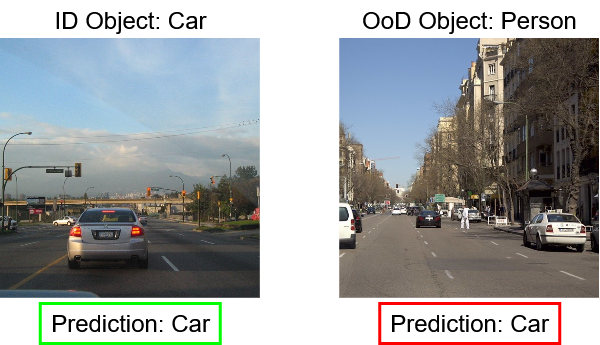
\includegraphics[width=0.9\linewidth]{figures/importance_example_1}

  \caption{OOD detection is a critical ML component necessary in many applications. Inability to identify unknown or unfamiliar data during use could lead to disastrous consequences. It is not enough for ML models to learn ID data, they must be designed with awareness of OOD data.
  }
  \label{fig:intro-ood_importance}
\end{figure}

%In practice, OoD detection has been recognized as a critically important component in myriad applications. In autonomous driving, several studies have studied using OoD detection for more accurate vehicle detection in images and identifying sources of road sign misclassification \cite{nitsch2021out,eykholt2018robust,geiger2012we,muhammad2020deep}. An example of the potential importance of OoD detection in autonomous driving is presented in Figure \ref{fig:intro-ood_importance}. With OoD detection, an ML model could identify the sudden OoD sample (right image) and, for example, activate a failsafe maneuver in order to avoid a catastrophic accident. In robotics, important uses of OoD detection include detecting sensor anomalies and environment-based behavior adaptation \cite{falcini2017deep,farid2022task}. In these cases, OoD detection can be used as a filter for noisy or malformed sensor readings to improve control of robots or prevent inappropriate actions in critical application environments. Benefits have also been noted in the related field of industrial automation, with one particular noteworthy study demonstrating use of OoD detection for identifying damaged products \cite{bergmann2019mvtec}. Studies in medical diagnosis have also identified beneficial applications of OoD detection via identification of abnormal growths, lesions, etc. as well as improving intelligibilty for patient transparency and trust \cite{caruana2015intelligible,schlegl2019f}. Further examples of OoD detection applications can be found in relevant works \cite{yang2021generalized,farid2022task,filos2020can,zhang2021out}.
\gls{ood} detection has already been tested in real-world applications, exhibiting critical importance across myriad settings. One application area with tangible effects is autonomous driving. Studies have investigated the use of \gls{ood} detection for vehicle detection in images and explaining sources of road sign classification mistakes \cite{nitsch2021out,eykholt2018robust,geiger2012we,muhammad2020deep}. An example of the importance of \gls{ood} detection in autonomous driving is illustrated in \ref{fig:intro-ood_importance}. \gls{ood} detection allows ML models to identify sudden \gls{ood} samples (right image), enabling intelligent responses to such situations, e.g. engaging failsafe maneuvers to avoid a catastrophic accident. Another application for \gls{ood} detection is robotics. \gls{ood} detection can be used to detect sensor anomalies or induce environment-based adaptations in robot behavior \cite{falcini2017deep,farid2022task}. In such applications, \gls{ood} detection acts as a filter for noisy sensor readings and improves robot control while preventing inappropriate actions in high-risk or resource-limited task environments. Other applications include industrial automation, where \gls{ood} detection has been evaluated for identification of damaged products \cite{bergmann2019mvtec}. In medical diagnosis, \gls{ood} detection has proven effective at detecting medical anomalies such as abnormal growths, lesions, etc. Additionally, applications improving the intelligibility of medical results for improved patient transparency and trust have leveraged \gls{ood} detection \cite{caruana2015intelligible,schlegl2019f}. More examples of \gls{ood} detection in real-world applications can be found in relevant surveys and research works \cite{yang2021generalized,farid2022task,filos2020can,zhang2021out}.

%\begin{abstract}
%Although out-of-distribution (OOD) detection has been extensively studied, it continues to face challenges in handling OOD data semantically similar to In-Distribution (ID) data. Part of the difficulty arises from the model's inability to learn superior ID class discriminative features. We propose to improve this by segmenting input images into \textit{foreground} and \textit{background} views and combining them with the original input image (original view) in a multi-view learning approach. We present a novel method, called \textbf{\sys}~(\textbf{C}ross-view \textbf{A}ttention of \textbf{S}egmented views for \textbf{O}OD \textbf{D}etection), that learns better discriminative information from all three views and subsequently, fuses them through a novel stacked cross-view attention mechanism to produce the final predictive feature representation. A feature-based OOD method is then applied to the final fused feature for OOD detection, giving major improvements over a range of strong baselines on various near- and far-OOD datasets.
%\sys achieves state-of-the-art performance in various experimental settings with challenging ID and OOD datasets. The \sys \textbf{codebase} is submitted in the supplementary materials.
%\end{abstract}
%
%Machine learning (ML) models have been largely built and deployed under the \textit{closed-world} assumption \citep{joseph2021towards}, where the test data distribution is assumed to be the same as the training data distribution. However, this assumption is often violated in real-world scenarios, as a deployed model may encounter test instances of classes not seen during training. To reliably operate in such \textit{open-world} settings \citep{liu2023ai}, ML models should not only recognize instances of known (or seen) classes, referred to as \textit{in-distribution} (ID) classes, but also detect instances of novel (or unseen) classes, referred to as \textit{out-of-distribution} (OOD) samples. This task is called \textit{OOD} \textit{detection}, which aims to detect OOD instances when the detector is trained only with the ID data. OOD detection has a wide range of applications, e.g., autonomous driving \citep{nitsch2021out},  %robotics \citep{muhammad2020deep}, 
%medical diagnosis \citep{schlegl2019f}, %industrial automation \citep{bergmann2019mvtec}, 
%etc. An excellent review can be found in \cite{yang2024generalized}.

% - (sec) near-OOD, examples for image and text
%  + most difficult
\section{Critical Challenges - Ambiguity in OOD Detection}

\begin{figure}
 \centering
 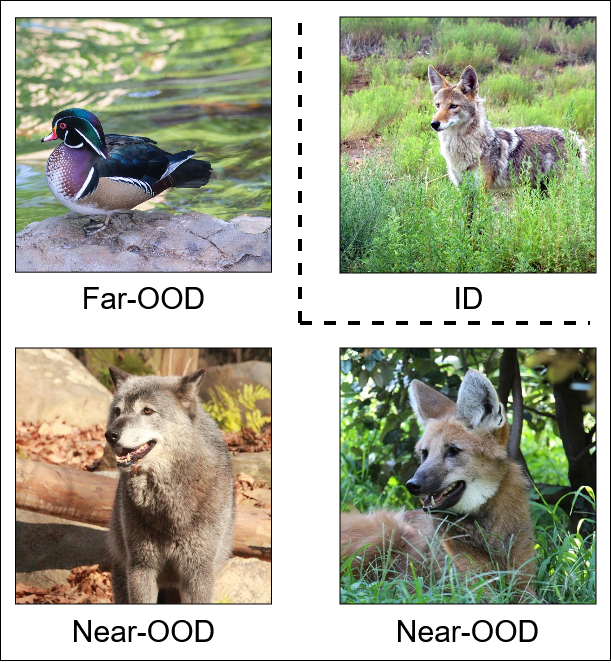
\includegraphics[width=0.9\linewidth]{figures/nearood_example}

  \caption{Detecting OOD samples that are similar to ID samples is a major challenge for OOD detection methods. Considering the coyote in the upper-right corner as the seen (ID) data during training, the bird in the upper-left corner is easy to detect as many features are significantly different (far-OOD). However, the wolf and other coyote sub-species are difficult to detect because they share many similar or overlapping features with the ID data (near-OOD).
  }
  \label{fig:intro-nearood}
\end{figure}

%Despite the importance of OoD detection, existing state-of-the-art methods underperform because they do not sufficiently learn representative information characteristic of ID data. This proposal introduces a novel method that seeks to address this issue and improve OoD detection performance by exploring the use of \textit{multiple views} of data to learn better characteristic ID information. Existing state-of-the-art OoD detection methods and their associated issues are detailed in Section \ref{sec:intro-relwork}. The research thesis, proposed method, and supporting evidence for its contribution are further presented in Section \ref{sec:propwork}. Additional directions for research involving multiple views and OoD detection are suggested in Section \ref{sec:future_work}.
%Although existing OOD detection methods have achieved good performance, they still struggle to detect near-OOD instances \citep{yang2022openood}%, winkens2020contrastive} 

%A significant challenge remaining for OOD detection is the detection of \emph{near-OOD} samples \cite{yang2022openood,winkens2020contrastive}. Near-OOD samples are generally defined as data samples that contain many features that are similar to (or perhaps even overlap) those of ID samples \cite{winkens2020contrastive}. Note that far-OOD samples are simply considered to be data samples with features that are significantly different from ID data features. Intuitively, near-OOD samples are difficult for discriminative classifiers to detect, as such models are designed to extract discriminative features from $\mathcal{D}_{id}$ and similar features in near-OOD data samples deceive the model. Thus, the problem is that existing OOD detection models do not learn \emph{discriminative features} that are sufficiently and distinctly representative of ID class objects. Instead, the deceptive features, henceforth referred to as \emph{spurious features} \cite{neuhaus2023spurious}, are included during learning. Spurious features are not guaranteed to be from the ID distribution and mislead models at test-time when OOD samples may be encountered \cite{ming2022impact,paullada2021data}. This problem is diminished in traditional classification learning as the \emph{i.i.d.} assumption assures that the identical training and test data distributions allow for both discriminative and spurious features to correlate with classes. In OOD detection, this guarantee does not exist, as the OOD (i.e. testing) data distribution is different from that of the ID (i.e. training) distribution $\mathcal{P}_{id}$. Learning class-relevant ID discriminative features is critical because they establish boundaries between ID classes and OOD instances in the feature space, enabling more accurate identification of ID target objects (and subsequently OOD data samples).
Despite the importance of \gls{ood} detection in developing ML systems for open-world settings, significant challenges remain. In particular, the ambiguity between \gls{id} data distributions and all possible \gls{ood} data in the \gls{ood} data distribution allows for extremely difficult cases where \gls{ood} data is similar to samples from the \gls{id} data distribution seen by the model. Consider the above example of the coyote and wolf in the nature preserve \gls{ood} detection application. During training, the ML model saw images of coyotes and learned feature information on coyotes in the \gls{id} data distribution. However, when a wolf appeared during testing, many features from the wolf were similar to or overlapped with those from the coyotes. Given the ML model had only seen animals like coyotes in the \gls{id} data, it would struggle to identify the wolf as an \gls{ood} data sample. This problem is exacerbated if different sub-species of coyotes are considered. If one sub-species of coyote is included in the \gls{id} data distribution and a different sub-species of coyote is encountered during test time, the ML model would have significant difficulty in detecting the different coyote species as \gls{ood}. \ref{fig:intro-nearood} illustrates this example. Here is another example from the text data domain. Imagine an ML model is trained to handle user queries on banking topics related to renewal of a card. The \gls{id} data contains many queries related to card renewal, such as \texttt{Why isn't my card available for use anymore? Did it expire?}, but the model encounters various \gls{ood} queries during testing. Some \gls{ood} queries may be clearly \gls{ood}, for example if the query is asking the model about a loan, e.g. \texttt{I'd like to be considered for a loan, what should I do?}. However, other \gls{ood} queries may be deceptively similar to the \gls{id} data distribution, closely aligning with the ``card renewal'' \gls{id} data. If an \gls{ood} query was asking the model about card cancellation, perhaps with \texttt{My card is close to expiring, can you make my card unavailable for further use?}, the ML model may have a hard time identifying the sample as \gls{ood} given its similarity to \gls{id} data it has seen.

These examples illustrate the challenge of \textbf{near-\gls{ood}} detection \cite{yang2022openood,winkens2020contrastive}. The definition of near-\gls{ood} samples encapsulates the above provided examples. \gls{ood} data that contain features similar to (including overlapping with) those in the \gls{id} data distribution are ``near-\gls{ood}'' \cite{winkens2020contrastive}. This also establishes the definition of \textit{far-\gls{ood}} samples, which are \gls{ood} data that are clearly different from data in the \gls{id} data distribution. Intuitively, near-\gls{ood} data is significantly more difficult for discriminative classifier ML models to detect, as such models are designed to extract and learn features from the \gls{id} data distribution \cite{rubinstein1997discriminative,liu2012discriminative}. As near-\gls{ood} data by definition contains features similar to \gls{id} data, they deceive the model and are harder to detect by nature of lying close to the discriminative decision boundaries learned by such models and methods. The source of the challenge for near-\gls{ood} data is thus in the limited ability of ML models to learn \textit{discriminative features} that sufficiently and distinctly represent the \gls{id} classes (which are an approximate simplification of the \gls{id} data distribution commonly used across the space of ML classification and \gls{ood} detection \cite{kim2015deep,wang2016machine,hendrycks2017baseline}). Instead, deceptive features, denoted as \textit{spurious features} \cite{neuhaus2023spurious}, are learned from the \gls{id} data. Spurious features are not guaranteed to exclusively belong to the \gls{id} data distribution, and learning of such features can mislead ML models during testing when near-\gls{ood} samples may be encountered \cite{ming2022impact,paullada2021data}.

Importantly, this problem is diminished in traditional classification task environments (including those under the \textit{closed-world} assumption) as the \textit{i.i.d.} assumption assures that the training and testing data distributions are identical. This allows for both discriminative and spurious features to correlate with data (and classes) across distributions, providing benefits for the model with no risk of misleading. However, in \gls{ood} detection, this assumption does not apply and thus the guarantee does not exist. The distribution of \gls{ood} data is not the same as the \gls{id} distribution. Spurious features can be present in the \gls{id} testing data \textit{and} the \gls{ood} testing data, which misleads the ML model into recognizing near-\gls{ood} samples with overlapping spurious features instead of detecting them as \gls{ood}. The solution is for ML models to learn \textit{\gls{id} class-relevant discriminative features} because they define distinctive boundaries in the embedding space between \gls{id} classes and \gls{ood} samples. This enables improved detection of \gls{ood} samples with respect to the learned \gls{id} classes and data distribution.

% - (sec) solution directions for image and text, requiring accessible/efficient AND effective
%  + issue is not just achieving good performance with near-OOD, need to also focus on designing solutions that are feasible for application
%  + this implies not only efficacy but efficiency and accessibility
%  + leveraging existing data, solutions, and models boosts accessibility
%  + tuning and pre-training/testing-only methods boost efficiency
%  + prompt-only boosts accessibility
\section{Real-World Solution Directions for Near-OOD Detection}

Solving the near-\gls{ood} detection problem in the context of the open-world setting not only requires the targeted leveraging of \gls{id} class-relevant discriminative features but also requires consideration of applying near-\gls{ood} detection-capable ML systems in real-world environments. From the perspective of a user, it is not only \textit{effectiveness} that is necessary but also \textit{efficiency} and \textit{accessibility} \cite{yuhas2021embedded,li2025secure,wang2025enabling}. Efficiency embodies the optimization of cost for a solution, encapsulating resource requirements with respect to time (data) space. Accessibility embodies the ease-of-use for any given application-side entity (be it developer or end-user). An \gls{ood} detection solution that is highly effective but is intractably expensive in time and computing resources is impossible to develop for and produce in a real setting. Likewise, a solution that requires significant user effort limits its applicability and indirectly reduces overall effectiveness.

\begin{figure}[t]
 \centering
 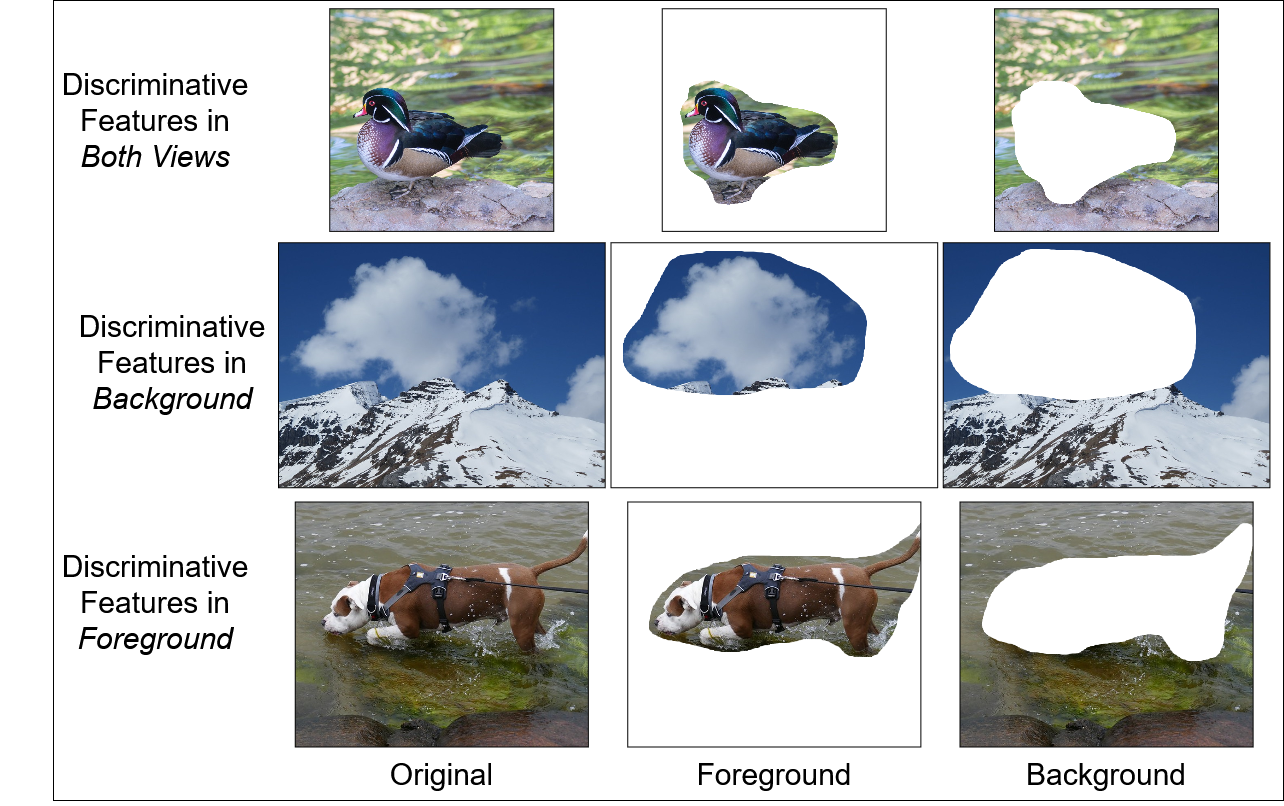
\includegraphics[width=0.95\linewidth]{figures/casod_mv_example}
  \caption{
  %\textcolor{red}{TODO: update} 
  %Foreground and background views contain different ID class-relevant discriminative features for class identification. 
  ID class-relevant discriminative features may appear in any (original, foreground, or background) view of an image, or even in multiple views. Leveraging of these features for OOD detection requires cross-view modeling. Graphic from \cite{politowicz2025casod}. %Segmented views can help models learn important view-specific features and fuse them appropriately.
  }
  \label{fig:intro-mvexample}
  %\vspace{-0.1cm}
\end{figure}

%~(see Sec. \ref{sec:results}). A primary reason is that they do not learn discriminative features that are characteristic of the main object in ID classes well because they consider an \textit{image as a whole}, including both class-relevant and class-irrelevant regions. This often makes them learn spurious or short-cut features \citep{neuhaus2023spurious}, misleading the OOD detection \citep{ming2022exploit}. Using \textbf{only} a \textit{single view} (i.e. the original input image) is thus often \textbf{not enough} for the learner to learn ID class-discriminative features effectively, especially considering challenging near-OOD instances. Extracting and leveraging multiple views (each providing different but complementary information) of the same image can help the learner to better recognize distinguishing characteristics of target object(s) and their relations with the context. Biological systems also support this notion -- it is hypothesized that humans use multiple views to identify what is being observed \citep{weiner2016anatomical}. 

%  + leveraging existing data, solutions, and models boosts accessibility
%  + tuning and pre-training/testing-only methods boost efficiency
%This paper proposes to segment each image into its \textit{foreground} and \textit{background} views and combine them with the original image for OOD detection\footnote{While other options for views, e.g.  crop, rotation \& noise, or image augmentation exist, we noted that the presence of discriminative feature and object's context can be well captured using foreground and background views, which in turn improves OOD detection effectively (see Sec. \ref{sec:disc-ablation}).}. Figure \ref{fig:onecol_vfp} shows examples of three original images and their corresponding foreground and background views. We observe that either the foreground or the background and sometimes both (as in the original image) can contain critical ID class-discriminative features \cite{xiaonoise}. %zhu2017object,xiaonoise}. 
%For example, in Figure \ref{fig:onecol_vfp}, the \textit{Dog}-class image discriminative (object) features are primarily in the foreground while the \textit{Mountain}-class features are primarily in the background. The \textit{Duck}-class image features are in both, with the background water and foliage containing well-separated semantic context in the original view. Thus, depending on the class, all three views becomes important and can contribute in different proportions in the overall learning of the ID class-discriminative features. It is important to note that, although the original image (i.e., original view) contains all information present in the foreground and background views, it often becomes hard for learners to \textit{automatically isolate these views} (and the discriminative information they contain) during feature learning in a \textit{single-view learning framework}. Thus, by segmenting the image into three views (i.e., \textit{original}, \textit{foreground} and \textit{background}), we encourage the learner to explicitly consider useful information from different views and fuse them effectively, resulting in better discriminative feature representation for OOD detection.

%Overall, this isolation of class-relevant discriminative features facilitates learning of only discriminative features informative on ID class objects while simultaneously separating spurious features that otherwise mislead models. Observations in biological systems support the viability of this notion: it has been hypothesized that humans use multiple views of objects, scenes, etc. to perform rapid visual identification \cite{weiner2016anatomical,vuilleumier2002multiple}. Furthermore, foreground-background views are actively considered in biological systems \cite{vuilleumier2002multiple,weiner2016anatomical}, in image processing literature \cite{lin2021real}, and in industry (e.g. autonomous driving) \cite{drygala2022background}, making this approach relevant for modern applications and technology. Despite this, there has been little investigation into the intersection of multi-view data and OOD detection.
When considering the image data domain, a major obstacle to realistic near-\gls{ood} detection is the requirement of significant computational processing. Training expensive image-processing ML models demands significant resources and time-consuming curation of additional data \cite{houlsby2019parameter,hu2021lora,ridnik2021imagenet}. However, these demands can be mitigated through the use of existing resources that also provide additional information beneficial to \gls{ood} detection. For example, existing research in biological systems suggests that humans use multiple views, or alternative augmentations of an image, to identify what is being observed \cite{weiner2016anatomical,vuilleumier2002multiple}. Extracting and leveraging multiple views of an image, each containing different complementary information, could help ML models learn to better recognize distinguishing features of \gls{id} data via the contextual relationships across views. Take \ref{fig:intro-mvexample} as an example. Three original images and their corresponding foreground and background views are depicted, each on their own row. The \textit{Dog}-class image's discriminative features (i.e. those representing the object of ``Dog'') are primarily in the foreground and the separate views isolate these features from the background. The \textit{Mountain}-class image's discriminative features are primarily in the background and the separate views instead isolate these features from the foreground. In both cases, the corresponding view with discriminative features provides additional context that correlates with the original image, reinforcing the features to learn for the \gls{id} data distribution and removing spurious features. This benefit is not isolated to exclusive foreground or background cases. The \textit{Duck}-class image's discriminative features are in both views, with the water and foliage in the background containing informative semantic context that well-separates the class in the \gls{id} data space. Depending on the class, all three views may be important and can contribute to learning of \gls{id} class-relevant discriminative features in different proportions. This provides intuitive benefits over otherwise-equivalent single-view methods (i.e. which only use the original image) which \textit{must} include spurious features with discriminative features in the input, increasing the load on the model during learning to separate the discriminative features in addition to learning them. The \textit{existence of segmented datasets}, including \textit{efficient segmentation models}, establishes a justification for the considered novel \gls{ood} detection approach leveraging multiple foreground and background views by eliminating additional work in procuring such data \cite{lin2021real,drygala2022background,jocher2020ultralytics,qin2020u2}. Further efficiency and accessibility can be embodied by using existing \textit{pre-trained models} and \textit{parameter-efficient fine-tuning} to avoid expensive training costs with impractically high resource demands \cite{hu2021lora,sun2022out,chen2021empirical}. This motivates the development of \gls{sys} \cite{politowicz2026improving}, presented in detail in Chapter \ref{diss_casod} with additional supporting material preceding it in Chapter \ref{diss_mvood_init}.

%\textcolor{blue}{An example of how this isolation benefits OOD detection is presented in TODO( - figure). For the ID sample (left column), the original and foreground views contain the class-relevant ID discriminative features, demonstrated by the recognition of the ID target object and accurate classification. For the simple far-OOD  sample (middle column), all views are very different from the ID sample, with little presence of spurious features. However, for the hard near-OOD samlpe (right column), the features in the original and foreground views are \emph{spurious}, i.e. similar to those of the ID sample. This misleads both views to give high confidence (low OOD scores) to the OOD sample. Only the background view contains features that are significantly different from the ID sample features, resulting in low confidence (high OOD score) and successful detection of the OOD sample.} 

%  + leveraging existing data, solutions, and models boosts accessibility
%  + prompt-only boosts accessibility
For the text data domain, a similar obstacle and solution approach exists. With the advent of large language models (LLMs), application of ML systems is accelerating with increasing demands for more powerful and effective models \cite{angrisani2026gaps,minaee2024large}. However, training such LLMs requires an astronomical amount of computing resources, data, and power. There are consequences for these demands that inspire approaches avoiding the need for training \cite{ding2024sustainable}. Instead, with the known abilities of LLMs to embody and utilize learned pre-trained knowledge \cite{kumar2025llm}, it would be ideal if the benefits of near-\gls{ood} detection could be realized using \textit{only the LLM itself}. That is, implementing effective near-\gls{ood} detection without requiring any sort of interfacing with the LLM's components or underlying outputs (i.e. non-text generation outputs). This inspires the idea of using only \textit{prompts} to induce reasoning in the LLM leading to principled detection of a test input as \gls{id} or \gls{ood}. With the extensive knowledge embedded in LLMs from pre-training, extraction of the discriminative features in the test input relative to the discriminative features of the \gls{id} data distribution is feasible \cite{kumar2025llm,wang2024beyond}. Comparison of the resultant sets of discriminative features through alignment of the various similarity spaces defined by these features, e.g. lexical (comparing words and phrases) and semantic (comparing meanings), informs the weighting of the test input between \gls{id} and \gls{ood}. By limiting the solution to only a prompt, an LLM's basic interface, and the LLM's response, near-universal accessibility is guaranteed, requiring only access to an LLM and some data. This further guarantees efficiency as no training is required. This motivates the development of \gls{syst} \cite{politowicz2026achieving}, presented in detail in Chapter \ref{diss_atpo}.

% - thesis statement: OOD detect, particularly near-OOD detect, is improved in the image domain via fg-bg segmented images in multi-view CVCA and in the text domain via prompt-only, embodying not only performance effectiveness but also efficiency and accessibility

%The primary argument in this proposal is that the use of a single view (i.e. the input image data sample) is not optimal for the learning of discriminative features. Note that for the rest of this proposal, only the domain of image data is considered. Spurious features are included in the sample and interfere with the class-relevant discriminative semantic features necessary for OOD detection. Instead, explicitly separating foreground discriminative features and background features allows for OOD detection models to learn from data with isolated class-relevant information in images. 
%The problem of Out-of-Distribution (OOD) detection has been thoroughly researched but continues to underperform in "near-OOD" settings, where OOD data may be very similar or inseparable from in-distribution (ID) data. The problem is that current state-of-the-art OOD detection methods fail to learn and utilize ID class-representative discriminative features effectively, while simultaneously demanding inaccessible amounts of resources. This thesis presents two OOD detection methods that exhibit state-of-the-art performance in near-OOD settings, one in the image data domain via the use of multi-view cross-attention processing of segmented images, and one in the text data domain using efficient and accessible prompt-only detection via alignment and scoring. The first approach leverages the segmented data and segmentation models to employ a multi-view method for image-based OOD detection, denoted as Cross-view Attention of Segmented views for OOD Detection (CASOD). Through the use of a pre-trained model and a novel cross-view correlation attention fusion architecture, discriminative features are learned across the original image and a foreground and background view, resulting in a highly informative ID class-relevant feature space. Utilizing distance-based OOD detection methods, CASOD achieves state-of-the-art performance over previous OOD detection baselines across a number of academically- or publicly-available datasets, including ImageNet, NINCO, SSB-Hard, iNaturalist, Textures, OpenImage-O, Places365, Species, and SUN. In particular, OOD detection performance on near-OOD datasets is shown to significantly improve. The second approach utilizes the inherent knowledge and reasoning capabilities in large language models (LLMs) to solve the task of prompt-only OOD detection, which requires only the use of text-prompting for OOD detection with no access to LLM components, logits, or outputs and no fine-tuning. Through prompting LLMs to perform lexical and semantic alignment before giving an OOD score for the input, OOD detection on academically- or publicly-available near-OOD datasets, including the Banking, CLINC, StackOverflow, 20NewsGroups, Dbpedia, and Snips datasets, can be significantly improved. Experiments demonstrate that this method, denoted as Alignment-based Thresholding for Prompt-only OOD detection (ATPO), not only outperforms the previous prompt-only OOD detection method but also outperforms strong traditional OOD detection methods with access to LLM features and logits.
\textit{\underline{Thesis Statement:}}
This thesis demonstrates the state-of-the-art effectiveness of two OOD detection methods that were proven against near-OOD datasets in experiments against recent, competitive baselines while additionally fulfilling efficiency and accessibility requirements for real-world application. The first method focuses on the image data domain and utilizes multi-view processing of segmented foreground and background views to learn ID class-relevant discriminative features via a novel cross-view correlation attention feature fusion architecture. Usage of a pre-trained model with parameter-efficient fine-tuning, on top of a fast segmentation model, maintains low computational complexity and simple interfacing between image data and segmented views. Efficient leveraging of segmented foreground and background views results in improved near-OOD detection performance in challenging experimental settings. The second method investigates OOD detection in the text data domain through the use of only text prompts with no complex model components, ML programming expertise, data curation, or model training. Through the induction of lexical and semantic alignment-based reasoning in LLMs, effective near-OOD detection across a variety of settings can be achieved through the processing of scores informed by the ID data. By requiring only a prompt and an LLM with no training, any sort of user barrier is removed ensuring accessibility and efficiency.
\chapter{Background}
\label{diss_bkgd}

\section{Out-of-Distribution Detection}
\label{sec:bkdg-ooddetect}

%(ood detection task definition)

%An ID training set $\mathcal{D}_{ID} = \{(\mathbf{x}_i, y_i)\}^{N}_{i=1}$ contains samples $x_i \in \mathcal{X}_{ID}$ and associated labels $y_i \in \mathcal{Y}_{ID} = \{1,2,\dots,C\}$ drawn from an ID distribution $P_{ID}(X, Y)$, i.e. $\mathcal{D}_{ID} \sim P_{ID}$. In the open-world problem setting, an OOD space also exists $\mathcal{D}_{OOD} = \{(\mathbf{x}_i), y_i\}^{L}_{i=1}$ with corresponding samples $x_i \in \mathcal{X}_{OOD}$ and some unknown OOD label $y_i \in \mathcal{Y}_{OOD} = \{y | y \notin \mathcal{Y}_{ID}\}$, drawn from OOD distribution $P_{OOD}(X, Y)$. Given a test sample $x'$, the goal of OOD detection is to identify if the test label $y' \in \mathcal{Y}_{ID}$ or $y' \in \mathcal{Y}_{OOD}$. A classification model $f$ is used as an OOD detector model $G$ in the following formulation
%\begin{equation}
%  G(x', f) =
%  \begin{cases}
%    1 \text{\ (OOD),} & \text{$S(x'; f) \geq \lambda$} \\
%    0 \text{\ (ID),} & \text{$S(x'; f) < \lambda$} \\
%  \end{cases}
%\end{equation}
%where $S$ is a scoring function and $\lambda$ is a threshold. In research, the threshold is often not used in evaluation as it depends on the application. Instead, a ranking is produced based on the $S$ scores to measure the Area Under the Receiver Operating Characteristic curve (AUROC). 

%For $\mathcal{D}_{id}$, the input space is denoted as $\mathcal{X}$ and the space of all ID class labels is given as $\mathcal{Y} = \{1, 2, ... , R\}$, where $R$ is the number of classes. The ID dataset $\mathcal{D}_{id}$ is drawn \emph{i.i.d.} from the joint data distribution $P_{\mathcal{X} \mathcal{Y}}$. Let the ID distribution $\mathcal{P}_{id}$ be the marginal distribution of $P_{\mathcal{X} \mathcal{Y}}$ on $\mathcal{X}$. Given \emph{only} $\mathcal{D}_{id}$, an OOD detection model detects if an input image data sample $x'$ is from the ID distribution $\mathcal{P}_{id}$ or not (i.e. the data sample is from the OOD distribution containing all other data samples). Typically, this detection is represented using a decision $G_{\lambda}(x)$, formulated as a level set estimation:
%\begin{equation}
%\begin{aligned}
%  G_{\lambda}(x) =
%  \begin{cases}
%        \text{ID}     & M(x) \geq \lambda \\
%        \text{OOD}    & M(x) < \lambda \\
%  \end{cases}
%\end{aligned}
%\end{equation}
%with OOD score $M(x)$ for sample $x$ and user-defined threshold $\lambda$. However, the OOD detection literature more frequently makes use of the area under the receiver operating characteristic (AUROC) score \cite{bradley1997use,hendrycks2017baseline,lee2018simple} to eliminate reliance on a threshold \cite{hendrycks2017baseline}. In this case, the AUROC score is constructed using the OOD score $M(x)$ for sample $x$ and label $1$ for ID data samples and $0$ for OOD data samples. In this paradigm (and henceforth in this proposal), the OOD score $M(x)$ is \textit{higher} for samples identified as \textit{more ID} and $M(x)$ is \textit{lower} for samples identified as \textit{more OOD}. %\textcolor{blue}{explicitly say that higher is less ood and vice versa?}
An ID training dataset $\mathcal{D}_{ID} = \{(x_i, y_i)\ |\ x_i \in \mathcal{x}_{ID},y_i \in \mathcal{Y}_{ID}\}_{i=1}^N$ is composed of samples $x_i \in \mathcal{X}_{ID}$ and labels $y_i \in \mathcal{Y}_{ID} = \{1,2,\dots,C\}$ for number of ID samples $N$ and number of ID classes $C$. $\mathcal{D}_{ID}$ is drawn \emph{i.i.d.} from an ID distribution $P_{ID}(X, Y)$, i.e. $\mathcal{D}_{ID} \sim P_{ID}$, which is the marginal distribution of joint data distribution $P_{\mathcal{X} \mathcal{Y}}$ on $\mathcal{X}_{ID}$. There also exists the OOD marginal distribution $P_{OOD}$ on OOD data $\mathcal{X}_{OOD}$ and unknown OOD labels $\mathcal{Y}_{OOD}$. An OOD dataset $\mathcal{D}_{OOD} = \{(x_i)\ |\ x_i \in \mathcal{X}_{OOD},y_i \in \mathcal{Y}_{OOD}\}^{L}_{i=1}$ is drawn from the OOD distribution $\mathcal{D}_{OOD} \sim P_{OOD}$ and contains samples $x_i \in \mathcal{X}_{OOD}$ with labels $y_i \in \mathcal{Y}_{OOD} = \{y | y \notin \mathcal{Y}_{ID}\}$ for number of OOD samples $L$.

The OOD detection task is, given \emph{only} $\mathcal{D}_{ID}$ and a test sample $x'$, identify if the test label $y' \in \mathcal{Y}_{ID}$ or $y' \in \mathcal{Y}_{OOD}$. An OOD detection model $G$ uses an ML model $f$ in the following formulated level set estimation:
\begin{equation}
  G(x', f) =
  \begin{cases}
    1 \text{\ (OOD),} & \text{$S(x'; f) \geq \lambda$} \\
    0 \text{\ (ID),} & \text{$S(x'; f) < \lambda$} \\
  \end{cases}
\end{equation}
for scoring function $S(\cdot)$ and user-defined threshold $\lambda$. Of note is that the OOD score $S$ is \textit{higher} for samples identified as \textit{more ID} and $S$ is \textit{lower} for samples identified as \textit{more OOD}.

%{\color{red}near- vs far-OOD definitions or explanation}

\section{Metrics}
%However, the OOD detection literature more frequently makes use of the area under the receiver operating characteristic (AUROC) score \cite{bradley1997use,hendrycks2017baseline,lee2018simple} to eliminate reliance on a threshold \cite{hendrycks2017baseline}. In this case, the AUROC score is constructed using the OOD score $M(x)$ for sample $x$ and label $1$ for ID data samples and $0$ for OOD data samples. In this paradigm (and henceforth in this proposal), the OOD score $M(x)$ is \textit{higher} for samples identified as \textit{more ID} and $M(x)$ is \textit{lower} for samples identified as \textit{more OOD}.
Several metrics have been proposed to measure the performance of OOD detection methods \cite{lu2024recent}:
\begin{itemize}
    \item \textbf{Area Under the Receiver Operating Characteristic Curve (AUC).} This metric quantifies the model likelihood of assigning higher scores to ID samples with respect to scores of OOD samples. AUC correlates with the model's ability to correctly rank ID samples higher than OOD samples. A \textbf{higher} AUC is indicative of better OOD detection performance.
    \item \textbf{False Positive Rate at 95\% True Positive Rate (FPR95).} This metric quantifies the false positive rate (FPR) at the value where the true positive rate (TPR) becomes 95\%. It measures the amount of OOD samples incorrectly classified as ID. FPR95 correlates with an OOD detection model's likelihood of false detections under strict ID detection requirements. A \textbf{lower} FPR95 is indicative of better OOD detection performance.
    \item \textbf{Area Under the Precision-Recall Curve (AUPR).} This metric quantifies a combination of model precision and recall. Two versions of AUPR exist: one where precision and recall is considered for ID data as the ``correct'' class of interest (AUPR-IN) and one where OOD data is considered as the ``correct'' class of interest (AUPR-OUT). AUPR is particularly effective at measuring OOD detection performance under severe ID-OOD data imbalance. AUPR correlates directly with the model's ability to correctly classify ID (or OOD) data. A \textbf{higher} AUPR is indicative of better OOD detection performance.
    %\item \textbf{Detection Error (DE).} This metric quantifies a combination of model precision and recall. Two versions of AUPR exist: one where precision and recall is considered for ID data as the ``correct'' class of interest (AUPR-IN) and one where OOD data is considered as the ``correct'' class of interest (AUPR-OUT). In particular, AUPR effectively measures OOD detection performance under severe ID-OOD data imbalance. AUPR correlates directly with the model's ability to correctly classify ID (or OOD) data. A \textbf{higher} AUPR is indicative of better OOD detection performance.
\end{itemize}

Of note is that the OOD detection literature more frequently makes use of the AUC score \cite{bradley1997use,hendrycks2017baseline,lee2018simple}. AUC covers general model performance and avoids reliance on a user-defined threshold which may be application- or domain-dependent \cite{hendrycks2017baseline}. This thesis likewise prioritizes AUC as the predominant OOD detection metric but other metrics are reported in varying capacities as needed to illustrate robustness.

\section{Relevant OOD Detection Methods}

\subsection{Maximum Softmax Probability}

The paper proposing Maximum Softmax Probability (MSP) \cite{hendrycks2017baseline} is widely considered to be the work spawning the OOD Detection field. MSP uses a classification model $f$ and treats the predicted probability distribution, $\text{softmax}(\hat{y})$, as a representation of model confidence in the sample $x$ under consideration, where ``$\text{softmax}$'' is the softmax function and $\hat{y} = f(x) \in \mathbb{R}^C$ is the predicted logits. The maximum probability is used as the OOD score
\begin{equation}
\begin{aligned}
    S_{MSP}(x,f) = \max_c\ \text{softmax}(f(x)), \\
\end{aligned}
\end{equation}
with $\max\limits_{c}$ indicating the maximum function over probabilities of classes $c \in C$. MSP stands as a simple OOD detection tool that remains as a reliable baseline, although much research has revealed limitations to the method \cite{hendrycks2019scaling} and proposed improvements \cite{sun2021react}.

\subsection{Mahalanobis Distance}
\label{sec:bkgd-md}

%The MD OoD score measures the distance between a sample and a Gaussian distribution. Maximum likelihood estimation is used to approximately fit class-conditional Gaussian distributions to each class in the training distribution. The empirical class means $\hat{\mu}_{c}$ and covariance matrix $\hat{\Sigma}$ are calculated from the training dataset $\mathcal{D}_{id}$ using some feature extractor $\phi$
%\begin{equation}
%\begin{aligned}
%    \hat{\mu}_{c} & = \frac{1}{N_{c}} \sum_{i:y_{i}=c} \phi(x_{i}) \\
%    \hat{\Sigma} & = \frac{1}{N} \sum_{c} \sum_{i:y_{i}=c} (\phi(x_{i}) - \hat{\mu}_{c}) (\phi(x_{i}) - \hat{\mu}_{c})^\top \\
%\end{aligned}
%\end{equation}
%where $N_{c}$ is the number of samples in class $c$. For \sysa, the feature extractor $\phi$ is replaced with the MVCNN pipeline, using the fused feature $z_{fused}$ to construct the empirical class means and covariance matrix. Given a test instance $x'$, \sysa extracts the test fused feature $z'_{fused} = \mathcal{G} (\Phi_{V}(x'_{V}), s) $ ($V = \{org, fg, bg\}$) and computes the distance between it and the nearest class-conditional Gaussian distribution, resulting in the final MD OoD score
%\begin{equation}
%\begin{aligned}
%     M_{MD}(x') = \max_{c} (-(z_{fused}' - \hat{\mu}_{c})^\top \hat{\Sigma}^{-1} (z_{fused}' - \hat{\mu}_{c})) \\
%\end{aligned}
%\end{equation}
Mahalanobis Distance (MD) \cite{lee2018simple} is considered the original distance-based OOD detection method, measuring the distance between a sample $x$ and Gaussian distributions representing ID data in the feature space. MD first computes class-conditional Gaussian distributions for each ID class in the training distribution. This is intractable as it cannot be assumed that any model has access to the entire ID training data distribution. The authors of MD propose instead to approximately fit the ID class Gaussian distributions using maximum likelihood estimation over the available training data and tied covariance.

Specifically, empirical class means $\hat{\mu}_{C} = \{\hat{\mu}_{c}\}_{c=1}^{C}$ and a single, shared covariance matrix $\hat{\Sigma}$ are computed from the training dataset $\mathcal{D}_{id}$ using some feature extractor $\phi$
\begin{equation}
\begin{aligned}
    \hat{\mu}_{c} & = \frac{1}{N_{c}} \sum_{i:y_{i}=c} \phi(x_{i}) \\
    \hat{\Sigma} & = \frac{1}{N} \sum_{c} \sum_{i:y_{i}=c} (\phi(x_{i}) - \hat{\mu}_{c}) (\phi(x_{i}) - \hat{\mu}_{c})^\top. \\
\end{aligned}
\end{equation}
$N_{c}$ is the number of samples in class $c$ and sample $x_{i} \in \mathcal{D}_{ID}$.

Given the class means $\hat{\mu}_{C}$ and covariance matrix $\hat{\Sigma}$, the MD OOD score is calculated using the feature vector $z' = \phi(x')$ for test sample $x'$
\begin{equation}
\begin{aligned}
     S_{MD}(x',\phi) = \max_{c} (-(z' - \hat{\mu}_{c})^\top \hat{\Sigma}^{-1} (z' - \hat{\mu}_{c})). \\
\end{aligned}
\end{equation}
$\max\limits_{c}$ again indicates the maximum function over classes $c \in C$. MD continues to demonstrate impressive performance in many OOD detection domains \cite{yang2022openood,zhang2023openood,ren2021simple}. Importantly, as MD is a distance-based OOD detection method that relies on features (also referred to as a ``feature-based OOD detection method'' in this thesis), its performance on OOD detection improves as the embedded feature space (henceforth referred to simply as ``feature space'') improves. That is, as the model learns increasingly discriminative, ID class-relevant features, ID sample features cluster into localized groups (according to class) with increasingly distinct separation in the feature space. MD accurately models this feature space and thus separates OOD sample features from ID sample features more clearly \cite{lee2018simple,sun2022out,ammar2024neco,fort2021exploring}. Orthogonal techniques that improve learning of features from data, e.g. data augmentation, also benefit MD (and other feature-based OOD detection methods) \cite{sun2022out,khosla2020supervised,hendrycks2022pixmix,yun2019cutmix}.

\begin{figure}
 \centering
 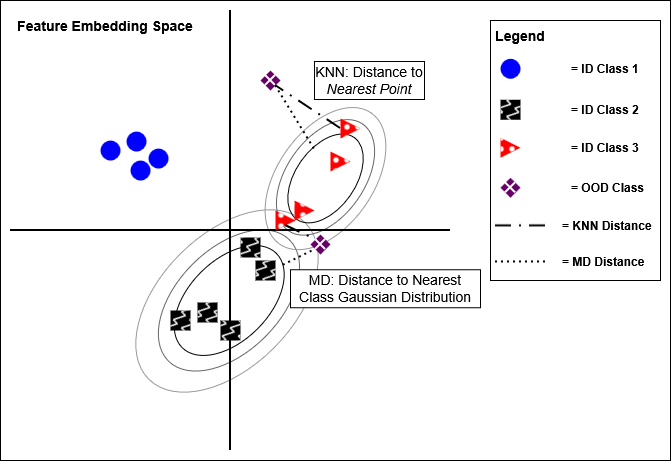
\includegraphics[width=0.9\linewidth]{figures/mdknn_example}
  \caption{Example illustration displaying the functionality of two distance-based OOD detection methods, namely MD and KNN, in the embedded feature space.
  }
  \label{fig:bkgd-mdknn}
\end{figure}

\subsection{k-Nearest Neighbors}

%The KNN OoD score is a non-parametric distance metric that uses the $k$-th nearest neighbor distance between a test image feature vector and feature vectors from the training dataset. Previous investigations have shown that the $L_{2}$ feature norms in ID data are larger than those from OoD data \cite{tack2020csi,huang2021importance}. To account for this, the feature vectors used by \sysa in the KNN score are the normalized fused features $\zeta = \frac{z_{fused}}{\lvert \rvert z_{fused} \lvert \rvert_{2}}$. Given normalized fused feature vectors $\mathbb{Z} = \{\zeta_{i}\}^{N}$ for the training dataset $\mathcal{D}_{id}$ and a test instance $x'$, the KNN OoD score is calculated as follows. First, the normalized fused feature vector $\zeta'$ for $x'$ is generated and the Euclidean distance of $x'$ from each $x_{i} \in \mathcal{D}_{id}$ is calculated as $\lvert \rvert \zeta_{i} - \zeta' \lvert \rvert_{2}$. Second, the features in $\mathbb{Z}$ are reordered according to distance to $\zeta'$, $\mathbb{Z}' = \{\zeta_{(i)}\}^{N}$. Finally, the KNN OoD score $M_{KNN}(x')$ for $x'$ is computed as the negation of the Euclidean distance to the $k$-th ID feature
%\begin{equation}
%\begin{aligned}
%    M_{KNN}(x') = -\lvert \rvert \zeta_{(k)} - \zeta' \lvert \rvert_{2}
%\end{aligned}
%\end{equation}
%Following the conventions of OoD scores (see Section \ref{sec:intro-relwork-ood}), higher (lower) scores $M_{MD}(x')$ and $M_{KNN}(x')$ for test instance $x'$ indicate the instance is less (more) OoD.
k-Nearest Neighbors (KNN) \cite{sun2022out} is another distance-based OOD detection method. However, it differs from MD in that it uses a non-parameteric distance metric. Specifically, KNN uses the $k$-th nearest neighbor distance between a sample $x$ and the training dataset feature vectors. An illustration of the similarities and differences between MD and KNN is in \ref{fig:bkgd-mdknn}.

ID training feature vectors are collected and normalized (per findings from a related investigation \cite{tack2020csi,huang2021importance}) from the training dataset $\mathcal{D}_{ID}$, $\mathcal{Z} = \{\zeta_{i}\}^{N}$ with $\zeta = \frac{z}{\lvert \rvert z \lvert \rvert_{2}}$ as the $L_2$ norm of feature vector $z$. The KNN OOD score is calculated using the normalized feature vector $\zeta'$ for test sample $x'$. Specifically, the Euclidean distances between $\zeta'$ and each $\zeta_i \in \mathcal{Z}$, $d_{KNN,i}(\zeta', \zeta_i) = \lvert \rvert \zeta_{i} - \zeta' \lvert \rvert_{2}$, is computed and ranked according to distance, $D_{KNN}' = \{d_{KNN,(i)}\}^{N}$ where $(i)$ represents the newly ordered position. The $k$-th Euclidean distance is used as the OOD score
\begin{equation}
\begin{aligned}
    S_{KNN}(x',\mathcal{Z},k) = -d_{KNN,(k)}(\zeta', \zeta_{(k)}). \\
\end{aligned}
\end{equation}
Note that KNN does not require the labels of the ID data, i.e. it is unsupervised. This has certain advantages in settings without guaranteed access to labeled data. As with MD, KNN improves as the feature space improves. Furthermore, KNN makes no assumptions about the distributions of data in the feature space.


\subsection{Virtual Logit Matching}

%ViM \cite{wang2022vim}, which has been shown highly effective \cite{zhang2023openood}. It divides a sample feature into a column subspace (CS) component and a null subspace (NS) component \cite{cook2020outlier,wang2022vim}. 
%ViM works as follows: Given the feature extractor $\phi$ of $f$, we define the feature $z = \phi(x)$ for input sample $x$. Further, the model $f$ can be retrieved as $f(x) = \mathbf{W} \phi(x) + \mathbf{b}$ with $\mathbf{W} \in \mathbb{R}^{d \times C}$ and $\mathbf{b} \in \mathbb{R}^{C}$ as the weight matrix and bias of a fully-connected layer. $d$ is the dimension of feature $z$. Following from ViM, the final fully-connected classification layer weight matrix $\mathbf{W}$ can be decomposed into a CS $W$ and an NS $W^{\perp}$. $W^{\perp}$ is unique in that it does not affect classification but it influences OOD detection due to the definition of NS. That is, the NS $W^{\perp} = \text{Nul} \mathbf{W}$ is the set of solutions satisfying $\mathbf{W} z = 0$. $z$ can be similarly decomposed into $z = z^{W^{\perp}} + z^{W}$ with $z^{W^{\perp}}$ and $z^{W}$ are projections of $z$ to the NS $W^{\perp}$ and CS $W$ respectively.
%Both ViM and NuSA observed that NS projections $z^{W^{\perp}}$ deviated significantly in OOD samples with respect to ID samples. NuSA exploited this observation by defining a score $\text{NuSA}(x) = \frac{\sqrt{\|z\| - \|z^{W^{\perp}}\|}}{\|z\|}$ and ViM defined a score $\text{ViM}(x) = \| z^{W^{\perp}} \|$ in comparison to predicted logits. However, both NuSA and ViM assume access to the sample feature $z$ and/or logits $\hat{y}$ to generate their respective OOD scores. 
%ViM observed that NS projections $z^{W^{\perp}}$ deviated significantly in OOD samples with respect to ID samples. ViM exploited this observation by defining a score $\text{ViM}(x) = \| z^{W^{\perp}} \|$ in comparison to predicted logits. However, ViM assumes access to the sample feature $z$ and logits $\hat{y}$ to generate the OOD score. 
Virtual Logit Matching (VIM) \cite{wang2022vim} is a hybrid OOD detection approach that uses both features and predicted logits to quantify an OOD score. VIM divides the feature vector $z$ of a sample $x$ into a column subspace (CS) component and a null subspace (NS) component before comparing the NS component to predicted logits $\hat{y}$.

The detailed procedure is as follows: given feature extractor $\phi$ of model $f$ and feature vector $z = \phi(x)$ for input sample $x$, the model can be further specified as $f(x) = W \phi(x) + b$ for classification linear layer weight matrix $W \in \mathbb{R}^{d \times C}$ and bias $b \in \mathbb{R}^{C}$, where $d$ is the dimension of feature vector $z \in \mathbb{R}^d$. $W$ can be decomposed into a CS $W_{cs}$ and an NS $W^{\perp}$. $W^{\perp}$ is unique in that it does not affect classification but it influences OOD detection due to the definition of NS. Specifically, the NS $W^{\perp} = \text{Nul}\ W$ is the set of solutions satisfying $W z = 0$. $z$ can be similarly decomposed into $z= z^{W^{\perp}} + z^{W_{cs}}$ with $z^{W^{\perp}}$ and $z^{W_{cs}}$ as projections of $z$ to the NS $W^{\perp}$ and CS $W_{cs}$ respectively.

NS projections $z^{W^{\perp}}$ in OOD samples deviate significantly with those in ID samples. To exploit this, VIM directly compares the NS projection with predicted logits. First, the NS projection is redefined as a virtual logit $\hat{y}_0 = \alpha \| z^{W^{\perp}} \|$, with $\alpha$ as a scaling parameter computed from virtual logits and maximum predicted logits of the ID data
\begin{equation}
\begin{aligned}
    \alpha = \frac{\sum_{i=1}^{N} \max_{j=1,\dots,C} \hat{y}_j^i}{\sum_{i=1}^{N} \| z^{W^{\perp}} \|}. \\
\end{aligned}
\end{equation}
Then, the virtual logit is concatenated to the predicted logits and a softmax is performed to retrieve the NS projection sample probability. The probability of the virtual logit is used as the OOD score
\begin{equation}
\begin{aligned}
    S_{VIM}(z,\hat{y}) = \frac{e^{\hat{y}_0}}{\sum_{i=1}^{N} e^{\hat{y}_i} + e^{\hat{y}_0}}. \\
\end{aligned}
\end{equation}
VIM has consistently shown state-of-the-art performance despite many later works proposing alternative approaches for OOD detection. The combination of feature and logits information increases the saliency of information for OOD detection in any given evaluated sample.

\section{Multi-View Processing}
\label{sec:bkgd-mvp}

%We segment each image $x$ in $\mathcal{D}_{id}$ into a foreground ($x_{fg}$) and a background ($x_{bg}$) view.  We still use the original image $x$ (from here notated as $x_{org}$ for clarity) as it contains integrated information. 
%The three views $x_{org}$, $x_{fg}$, $x_{bg}$ are fed to a view feature extractor 
%to learn features $z_{org}$, $z_{fg}$, $z_{bg}$. 
%
%Given the three views $x_{org}$, $x_{fg}$, $x_{bg}$ of image $x$, Each view $x_v$ (where $v \in \{org, fg, bg\}$) is fed to the ViT and its corresponding \textit{view-specific} Adapter at each block. The ViT and view-specific Adapter parameters for a view $v$ we denote as $\phi_{v}$ (with $\vec{\phi} = \{\phi_{org}, \phi_{fg}, \phi_{bg}\}$). The penultimate feature $z_v \in \mathbb{R}^{T \times d}$ is thus obtained via $z_v = \phi_v (x_v)$. 
%Finally, the three view features $z_{org}$, $z_{fg}$, and $z_{bg}$ are fused 
A multi-view dataset $\mathcal{D}_{MV} = \{(x_{MV,i}, y_i)\}$ contains set of labels $y_i$ and a set of associated multi-view samples $x_{MV,i}$. Each multi-view sample is composed of a set of \emph{views} $x_{MV,i} = \{x_{i,0}, x_{i,1}, \dots, x_{i,V}\}$ where $V$ is the number of views. Views are images, with each view being a copy of the original image under covariate or semantic shift (including no shift, i.e. the original image itself). That is, given some augmentation function introducing covariate or semantic shift $\mathcal{B}(\cdot)$, a view is defines as $x_{i,v} = \mathcal{B}(x_i)$ for original image $x_i$.% and with $v \in \mathbb{N}^V$.

Multi-view models process multi-view datasets by taking each view in a multi-view sample as input and calculating some representation coalescing information across the views as output. The multi-view model $f_{MV}$ may be considered as a set of individual-view models $f_{MV} = \{f_0, f_1, \dots, f_V\}$. Each view in a multi-view sample $x_{i,v}$ is processed by its corresponding individual-view model $f_v$. Note that  individual-view models can be the same, and thus shared. Outputs from each individual-view model are then coalesced in an operation referred to as ``\textbf{fusion}'', resulting in a collective output from the multi-view model $f_{MV}(x_{MV,i}) = \mathcal{U}(\{f_0(x_{i,0}),f_1(x_{i,1}),\dots,f_V(x_{i,V})\})$ for fusion operation (or embodying architectural module) $\mathcal{U}$.

\section{Prompting for OOD Detection}

%Since we aim to use verbal prompts only,
%we propose to extract the latent knowledge in LLMs for OOD detection using prompts to approximate the NS and CS of an input sample $x$ using tokens (words) generated by the LLM, following the prompts. Given a prompt template $\mathcal{P}$ and an input $x$, an input prompt is constructed $\mathcal{P} (x)$. A function $\text{Parse}_{\perp}(\cdot)$ is used to extract the set of tokens representing the approximate NS $\mathcal{T}_{\perp} = \{t_{\perp,1},t_{\perp,2},\dots,t_{\perp,n}\}$ and $\text{Parse}_{\mathcal{C}}(\cdot)$ is used to extract the set of tokens representing the approximate CS $\mathcal{T}_{\mathcal{C}} = \{t_{\mathcal{C},1},t_{\mathcal{C},2},\dots,t_{\mathcal{C},m}\}$ from the generated output of an LLM model $f_{LLM}$
%\begin{equation}
%\begin{split}
%	%\{z_{org+fg}, z_{org+bg}\} & = CVCA(z_{fg \rightarrow org}, z_{bg \rightarrow org})
%	\mathcal{T}_{\perp} & = g_{\perp} (x) = \text{Parse}_{\perp} (f_{LLM}(\mathcal{P} (x))) \\
%	\mathcal{T}_{\mathcal{C}} & = g_{\mathcal{C}} (x) = \text{Parse}_{\mathcal{C}} (f_{LLM}(\mathcal{P} (x))) \\
%\end{split}
%\end{equation}
%We share the prompt template and examples in Appendix \ref{sec:app-prompts}. Our proposed method for exploiting this verbalized form of decomposition-based OOD detection, \sys-ViM, uses two  phases.
A text dataset $\mathcal{D} = \{(x_{\text{text},i}, y_i)\}$ is composed of labels $y_i \in \mathcal{Y}_{ID}$ and text samples $x_{\text{text},i} \in \mathcal{X}_{\text{text}}$. Given a prompt template $\mathcal{P}$ and a text input $x_{\text{text}}$, a prompt $P$ is constructed $P = \mathcal{P}(x_{\text{text}})$ as input to a language model (LM), e.g. an LLM, for generation of a response to be used for OOD detection. Specifically, given prompt template $\mathcal{P}$, a parsing function $\text{Parse}(\cdot)$ is used to extract an OOD score $S$ from the output of LM $f_{LM}$
\begin{equation}
	S(x_{\text{text}},f_{LM}) = \text{Parse}(f_{LM}(\mathcal{P}(x_{\text{text}}))).
\end{equation}
The parsing function $\text{Parse}(\cdot)$ typically operates over the tokens generated from the LM $\mathcal{T} = f_{LM}(\mathcal{P}(x_{\text{text}}))$. In existing work, $\text{Parse}(\cdot)$ takes the form of an identity function detecting the presence of either an ID class token or the ``unknown'' token \cite{wang2024beyond}. That is, the baseline prompt-only OOD detection method uses parsing function
\begin{equation}
    \text{Parse}_{base}(\mathcal{T}) = -\mathbbm{1}_{\text{``unknown''} \in \mathcal{T}}.
\end{equation}

\section{Attention}
\label{sec:bkgd-attn}

\begin{figure}
 \centering
 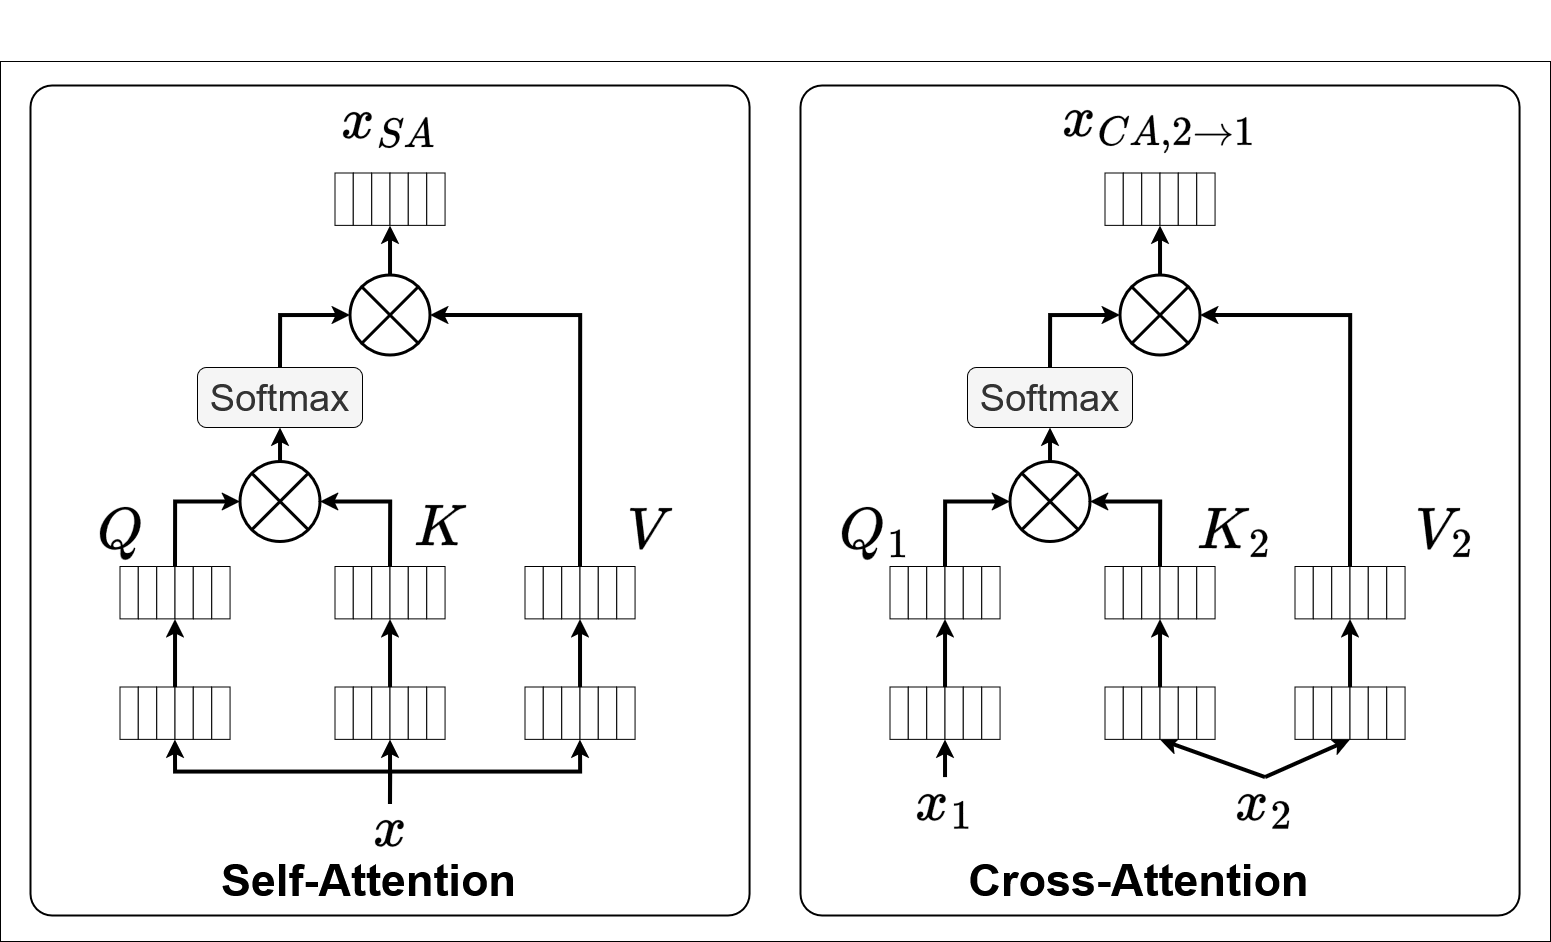
\includegraphics[width=0.9\linewidth]{figures/attention_diagram_simple}
  \caption{Attention allows models to extract and weight sections of an image during processing. Typically, two forms of attention are used, self-attention (left) and cross-attention (right).
  }
  \label{fig:bkgd-attn_example}
\end{figure}

%Attention \cite{} deserves its own introduction, both for its existing impact and for the role it plays in improved multi-view OOD detection. In general, there are two types of attention: self-attention and cross-attention. All attention mechanisms operate on a patch-style input format. Note that here we only consider image-based attention. That is, given an input image $x \in \mathbb{R}^{H \times W \times C}$, it is reshaped to have $T$ patches each of $d$ dimension, $x \in \mathbb{R}^{T \times d}$ where $d = P^2 \cdot C$ for patch resolution $P$. For an image input, this is analogous to sectioning the image $x$ into a grid of square image subsections of size $P$ before rearranging the sections into a sequence of $T$ length. Transformer models additionally prepend a class patch $x^0$ to the sequence and add position encoding to the patches \cite{dosovitskiy2020image}.
The Attention \cite{vaswani2017attention} mechanism has recently become a critical component in state-of-the-art neural network (NN)-based deep learning models \cite{dosovitskiy2020image}. There are two predominant types of attention: self-attention and cross-attention \cite{vaswani2017attention}. All attention mechanisms operate on a patch-style input format. Note that in this dissertation only image-based attention is considered. That is, given an input image $x \in \mathbb{R}^{\mathcal{I} \times \mathcal{J} \times \mathcal{K}}$ (where $\mathcal{I}, \mathcal{J}, \mathcal{K}$ refer to the image channel, width, and height dimensions respectively), traditionally the image is reshaped to have $T$ patches each of $d$ dimension, $x \in \mathbb{R}^{T \times d}$ where $d = P^2 \cdot \mathcal{I}$ for patch resolution $P$. For an image input, this is analogous to sectioning the image $x$ into a grid of square image subsections of size $P$ before rearranging the sections into a sequence of $T$ length. Transformer models additionally prepend a class patch $x^0$ to the sequence and add position encoding to the patches \cite{dosovitskiy2020image}. Examples of the types of attention, described below, can be found in \ref{fig:bkgd-attn_example}.

\textbf{Self-Attention:} An input $x$ is projected into a query $Q$, a key $K$, and a value $V$ using respective weight matrices $W_Q \in \mathbb{R}^{d \times d_k}$, $W_K \in \mathbb{R}^{d \times d_k}$, $W_V \in \mathbb{R}^{d \times d_v}$
\begin{equation}
\begin{aligned}
    Q & = x W_Q \\
    K & = x W_K \\
    V & = x W_V. \\
\end{aligned}
\end{equation}
$d_k$ and $d_v$ are projection dimensions selected by the user as hyperparameters. The query $Q$, key $K$, and value $V$ are used to calculate the attention as follows
\begin{equation}
\begin{aligned}
    \text{Attention}(Q,K) & = \text{softmax} (\frac{Q K^{\mathsf{T}}}{\sqrt{d_k}}) \\
    x_{SA}(\text{Attention},V) & = \text{Attention} \cdot V.
\end{aligned}
\end{equation}
%Attention effectively identifies which subsections of the image to attend to with respect to the optimization objective. The delineation of ``self-attention'' refers to the fact that the same input $x$ is used to compute each component ($Q$, $K$, $V$) for attention. Thus the attention mechanism references to and emphasizes components of itself when identifying important features. {\color{red}TODO; include figure showing what attention looks like} Self-attention can also be extended using multiple heads but this is out of scope of the dissertation \cite{vaswani2017attention}. The functionality is modular to any related method propositions.
Self-attention can also be extended to use multiple heads, but this is out of scope of the dissertation \cite{vaswani2017attention}.

\textbf{Cross-Attention:} Two inputs $x_1$ and $x_2$ are projected into a query $Q$, a key $K$, and a value $V$
\begin{equation}
\begin{aligned}
    Q & = x_1 W_Q \\
    K & = x_2 W_K \\
    V & = x_2 W_V, \\
\end{aligned}
\end{equation}
before attention is calculated as in self-attention
\begin{equation}
\begin{aligned}
    \text{Attention}(Q,K) & = \text{softmax} (\frac{Q K^{\mathsf{T}}}{\sqrt{d_k}}) \\
    x_{CA,2 \rightarrow 1}(\text{Attention},V) & = \text{Attention} \cdot V.
\end{aligned}
\end{equation}

\chapter{State of the OOD Detection Field}
\label{diss_relwork}

\section{Related Areas}
\label{sec:relwork}

%(related areas to ood: anomaly/novelty detection, open-set recog, etc.)

%There are several areas within the field of ML that are tangential to, and indeed have cross-pollinated with, OOD detection \cite{ghassemi2022comprehensive,cui2022out,shen2021towards}. \textit{Rejection} refers to the task of either accepting a given data sample as ``seen'' %during classification training 
%(analogous to ID data) or rejecting it as ``unseen'', typically with some associated cost \cite{cortes2016learning,geifman2017selective}. Works in this area parallel OOD detection in distinguishing between ID and OOD samples but focus more on optimizing for rejection costs \cite{cortes2016learning}. \textit{Anomaly detection} (or its close relative, \textit{novelty detection}) is the problem of detecting previously-unseen (i.e. anomalous or novel) data samples given some set of seen data \cite{tax2002one,liu2008isolation,andrews2016transfer}. Upon detection, the unseen data can then be either discarded, used to activate another behavior, or reserved for future training as a new task. Anomaly and novelty detection differ from OOD detection in that they do not consider the seen (ID) data for classification, instead treating the seen data as a whole solely for identifying unseen (OOD) data \cite{yang2021generalized}. OOD detection uses the classes inside of the ID data to better detect OOD data and often performs ID classification at the same time \cite{yang2022openood}. \textit{Open-set recognition} is a problem that somewhat overlaps with OOD detection. Methods in open-set recognition aim to simultaneously correctly classify known data encountered during training while also detecting unknown data at test-time \cite{scheirer2012toward,bendale2015towards,ge2017generative,neal2018open,scheirer2014probability}.
\gls{ood} detection as a domain of ML exists parallel to several other related fields, between which significant cross-pollination has occurred as ML has developed over time \cite{ghassemi2022comprehensive,cui2022out,shen2021towards}. The field of \textit{rejection} targets identifying and separating ``seen'' data samples (analogous to \gls{id} data) from ``unseen'' data samples, often using some cost to facilitate rejecting ``unseen'' samples during learning \cite{cortes2016learning,geifman2017selective}. Works in rejection are parallel to \gls{ood} detection but focus on optimizing for the aforementioned rejection cost instead of separating \gls{id} and \gls{ood} data \cite{cortes2016learning}. \textit{Anomaly detection} (or equivalently, \textit{novelty detection}) attempts to solve the problem of detecting data samples that have not been seen during training (i.e. anomalous or novel) \cite{tax2002one,liu2008isolation,andrews2016transfer}. Detected unseen data can be discarded or used in a variety of ways to facilitate additional procedures, such as future training as a new task. Anomaly and novelty detection differ only minutely from \gls{ood} detection. The primary difference is seen (\gls{id}) data and unseen (\gls{ood}) data are considered as whole collections in anomaly and novelty detection while \gls{ood} detection frequently leverages labels in \gls{id} data for detection \cite{yang2021generalized,yang2022openood}. In \textit{open-set recognition}, testing data is simultaneously classified and evaluated for similarity to known training data \cite{scheirer2012toward,bendale2015towards,ge2017generative,neal2018open}. The field overlaps with \gls{ood} detection.

%Other OOD detection-tangential fields in ML worth mentioning include \textit{uncertainty estimation} and \textit{causal representation}. The problem of uncertainty estimation in ML directly aims to quantify how uncertain a model is in a given data sample \cite{loquercio2020general,malinin2018predictive,malinin2019reverse}. %This can take the form of the complement to the maximum predicted class-distribution confidence produced by a model or some other metric estimating the model's recognition of the sample \cite{hendrycks2017baseline}. 
%This can take the form of an ML model's predicted confidence or some other metric estimating recognition of a sample \cite{hendrycks2017baseline}. Some methods in OOD detection make use of uncertainty estimation techniques to detect OOD samples at test-time \cite{hendrycks2017baseline,gal2016dropout,guo2017calibration}. %\textcolor{blue}{more could easily be added here if necessary} 
%Causal representation is a field that focuses on generating causal variables from observations that can then be used in causal graphs and reasoning \cite{scholkopf2021toward}. By using learned causal representations, models can infer whether encountered data samples are distributionally shifted (i.e. OOD) or not \cite{wang2022causal}. Another field similar to OOD detection is \textit{outlier exposure}, which uses ``outlier'' samples during training to explicitly learn what data should be considered as ``inliers'' (ID) or anomalies (OOD) \cite{hendrycks2018deep,yang2021generalized,chen2021atom,papadopoulos2021outlier}. This domain is not considered as directly comparable to OOD detection as it assumes access to OOD data during training, a violation of the OOD detection task definition. %\textcolor{blue}{TODO add outlier exposure here and emphasize it is not considered directly as OOD b/c they use OOD data}
Additional relevant fields tangential to \gls{ood} detection include \textit{uncertainty estimation} and \textit{causal representation}. ``Uncertainty'' in ML is a fundamental concept that quantifies the quality of a model's output, providing feedback on how uncertain a ML model is on a given data sample \cite{loquercio2020general,malinin2018predictive,malinin2019reverse}. With respect to \gls{ood} detection, this measure of uncertainty represents the model's confidence in the sample being \gls{ood} \cite{hendrycks2017baseline}. Uncertainty estimation underlies many state-of-the-art \gls{ood} detection methods \cite{hendrycks2017baseline,gal2016dropout,guo2017calibration}. Although less-directly related, causal representation nevertheless has shown value in \gls{ood} detection by learning causal representations and inferring if encountered data samples are \gls{ood} (i.e. distributionally shifted) \cite{scholkopf2021toward,wang2022causal}. \textit{Outlier exposure} (OE) is a prevalent tangential field that uses ``outlier'' data samples during training to learn differences between ``inlier'' (\gls{id}) and anomalous (\gls{ood}) samples \cite{hendrycks2018deep,yang2021generalized,chen2021atom,papadopoulos2021outlier,lioutlier,wei2024eat}. While OE solutions target the \gls{ood} detection problem, they are not directly comparable to non-OE \gls{ood} detection methods as they frequently assume access to \gls{ood} data during training. This violates the definition of the \gls{ood} detection task. However, recent work in OE has investigated generating synthetic outliers for training instead of assuming access to \gls{ood} data, a promising direction with great potential in realistic open-world applications \cite{gong2025out}. Of note is that \gls{ood} detection is not the same as \textit{\gls{ood} generalization}, which seeks to most effectively broadcast learned \gls{id} classes to potentially \gls{ood} testing data \cite{zangovercoming,li2023distilling,vogt2023robust}.

While the previous fields interleave with \gls{ood} detection, the field of \textit{continual learning} (CL) instead draws from \gls{ood} detection, utilizing it as a critical component in the conceptual and technical pipeline of CL. The task in CL is to incrementally learn a sequence of tasks \cite{thrun1995lifelong,hadsell2020embracing,chen2018lifelong}. It has been shown that the ability to understand when a new task has arrived fundamentally relies on \gls{ood} detection \cite{kim2022theoretical}. In the class-incremental learning (CIL) paradigm of CL, data is encountered over time but no indication is provided to the model regarding which task any given data sample belongs to. A CIL model must \emph{detect} if a data sample does not belong to previously encountered tasks - a problem that fits \gls{ood} detection \cite{kim2022multi,kim2023learnability}. CL stands as an example of how \gls{ood} detection plays an important role in open-world ML.

\section{OOD Detection Techniques}
\label{sec:relwork-ood}

\begin{figure}
 \centering
 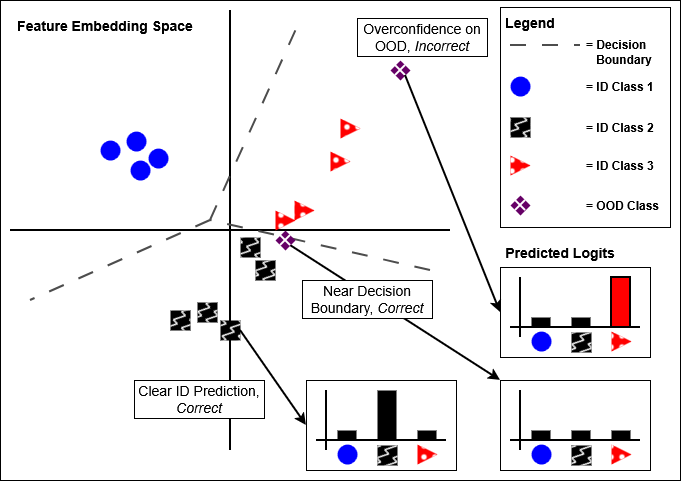
\includegraphics[width=0.9\linewidth]{figures/logits_describe}
  \caption{Example of the functionality of logits in detecting ID and OOD test samples. Overconfidence is a major issue with logits, incorrectly detecting the OOD sample in the upper right corner as ID.
  }
  \label{fig:relwork-logits_example}
\end{figure}

%(logit and confidence based methods, simple but subject to nn overconfidence and info loss)

%Initial attempts in OOD detection focused on leveraging ML model prediction outputs to measure model familiarity with encountered data samples. In what is often considered to be the seminal work in OOD detection, a neural network (NN) was trained to classify an ID dataset. Given a sample, the output logits of the NN %(resulting from processing the sample) 
%were converted to a prediction probability distribution using the softmax function %\textcolor{blue}{add a reference here, maybe say we will define it later and have a reference to the section} 
%and the maximum softmax probability (MSP) was treated as a measure of \emph{confidence} \cite{hendrycks2017baseline}. High MSP (confidence) values were characterized as a metric representing a low OOD score (i.e. more likely to be ID) while low MSP values were characterized as a high OOD score. This methodoloy was expanded upon in several directions, with some works directly using maximum logits as OOD scores \cite{hendrycks2019scaling}, normalizing the logits to reduce variance in predicted values \cite{wei2022mitigating}, or converting logits to energy values with less bias \cite{liu2020energy,wang2021energy}. Other research directions attempted to modify training procedures or adapt NN components to improve the utility of logits for OOD detection. The ODIN family of methods uses temperature scaling and input modification to estimate an OOD score based on how the logits change \cite{liang2017enhancing,hsu2020generalized}. Rectified Activations (ReAct) modulates NN intermediary layer outputs via clipping of activations, resulting in more distinguishable OOD logits \cite{sun2021react}. Generalize Entropy (GEN) modifies NN outputs using thresholded generalized entropy to reduce variance in predicted logits \cite{liu2023gen}. Further works leveraging logits for OOD detection have evaluated interpreting logits as density values \cite{abati2019latent,pidhorskyi2018generative,zong2018deep}, decomposed NN components for improved OOD detection with logits \cite{hsu2020generalized,huang2021mos,huang2021importance,devries2018learning}, utilized behaviors of NN weights to calibrate logits for OOD detection \cite{shama2019detecting,sun2022dice}, or investigated additional paradigms (prior networks \cite{malinin2019ensemble}, semantic representations \cite{shalev2018out}, classifier discrepancy \cite{yu2019unsupervised}) for improved logits-based OOD detection \cite{scheirer2012toward,smith1990extreme}. However, logits-based OOD detection methods are limited by two major factors. First, predicted logits inherently \emph{reduce the information} available in the model for identifying ID or OOD samples \cite{lee2018simple}. Second, NN models are known to be overconfident on predictions, regardless of if encountered samples are previously seen or unseen, significantly reducing their reliability for OOD detection \cite{nguyen2015deep,hendrycks2017baseline,wei2022mitigating,lee2018simple,sun2021react,paullada2021data}.
Preliminary exploration in \gls{ood} detection revolved around analyzing ML model predicted outputs for characterization of model familiarity with processed data samples \cite{yang2024generalized,lu2024recent} The seminal work in \gls{ood} detection trained an NN to classify \gls{id} data, then converted test data output logits into a probability distribution (using the softmax function). The maximum softmax probability (MSP) was treated as the measure of confidence in the sample being from the \gls{id} data distribution \cite{hendrycks2017baseline}. High MSP values were indicative of the sample being more likely \gls{id} (i.e. a \textit{low \gls{ood} score}) while low MSP values were indicative of the sample being more likely \gls{ood} (i.e. a \textit{high \gls{ood} score}). Future work innovated on this method in multiple ways. Some work elected to directly use logits for \gls{ood} scores \cite{hendrycks2019scaling}, others discovered the benefits of normalizing logits to reduce variance \cite{wei2022mitigating}, and promising advances have been made in converting model predictions from logits to energy measures with less bias \cite{liu2020energy,wang2021energy,chen2025dual}. Further investigations into the characterization of probabilistic classification models as energy models have leveraged architectural changes via Hopfield networks to more appropriately quantify energy-based \gls{ood} scores \cite{zhang2022out,hofmann2024energy,hofmannenergy,moriai2025rectified}. Alternative research directions instead have focused on improving model learning itself for \gls{ood} detection instead of limiting scoring to only the predicted outputs \cite{liu2024fast}. The family of ODIN \gls{ood} detection methods uses calibration (via temperature scaling) and modification of data inputs to estimate an \gls{ood} score based on changes in predictions \cite{liang2017enhancing,hsu2020generalized}. \gls{ood} detection from perturbing test inputs remains of interest, with recent investigations showing notable results \cite{chen2025leveraging}. Several works step further in this direction, using generative models and corruptions to estimate \gls{ood} scores \cite{lee2025hybood}. Rectified Activations (ReAct) clips the activations of NN intermediate layers, resulting in greater distinction between \gls{id} and \gls{ood} outputs \cite{sun2021react}. Generalized Entropy (GEN) uses thresholds on entropy functions of model outputs to reduce variance within \gls{id} and \gls{ood} outputs \cite{liu2023gen}. Adaptive Temperature Scaling (ATS) modulates temperature scaling in NN models to isolate \gls{id} predictions from \gls{ood} predictions \cite{krumpl2024ats}. Variational Rectified Activation (VRA) parameterizes ReAct and learns optimal clipping of activations to further optimize detection of \gls{ood} samples \cite{xu2024vra}. Adaptive Scaling (AdaScale) further builds on these ideas by identifying individual activation shifts between \gls{id} and \gls{ood} data, enhancing detection \cite{regmi2025adascale}. Other advances in logits-based \gls{ood} detection include interpreting predictions as density or entropy values \cite{abati2019latent,pidhorskyi2018generative,zong2018deep,yang2025eood}, decomposing NN components for improved logit characterization \cite{hsu2020generalized,huang2021mos,huang2021importance,devries2018learning,chen2023gaia,yu2023block,chen2024optimal}, and calibrating logits for \gls{ood} detection through analysis of NN weight trends during learning \cite{shama2019detecting,sun2022dice,canevaroadvancing,kalantransfer}. Additional logits-based paradigms include using prior networks \cite{malinin2019ensemble}, semantic representations \cite{shalev2018out}, ensembles \cite{yang2021ensemble,xu2024outofdistribution}, or optimizing classifier discrepancy \cite{yu2019unsupervised} for improved \gls{ood} detection \cite{scheirer2012toward,smith1990extreme}.

In modern \gls{ood} detection, it is recognized that logits-based methods are fundamentally limited by two major factors. First, logits \emph{reduce information quality} for \gls{ood} detection \cite{lee2018simple}. Second, it is well-recognized that NN classification models are \emph{overconfident on predictions}. That is, models are biased towards predicting higher confidences regardless of if the given data sample is \gls{id} or \gls{ood}. An example of overconfidence in \gls{ood} detection is shown in \ref{fig:relwork-logits_example}. The \gls{ood} sample in the upper right should be clearly \gls{ood} as it is far from any \gls{id} samples, but it is incorrectly considered \gls{id} due to overconfidence (represented as being clearly inside the \gls{id} class confidence region and far from any decision boundary). An additional non-trivial limitation is the assumption that prediction distributions learned by models are correct, while in practice this is not guaranteed \cite{liu2024rethinking,miao2024long}. This significantly reduces the capacity for models to perform \gls{ood} detection \cite{nguyen2015deep,hendrycks2017baseline,wei2022mitigating,lee2018simple,sun2021react,paullada2021data}.

%\textcolor{red}{TODO: add math and figures (can be ref to other works) here} % TODO overconfidence image maybe? LOW PRIO

%(self-supervised methods, powerful but very expensive, indirectly related to our ideas)

%A sub-direction of OOD detection methods attempts to resolve the overconfidence issue by exposing models to additional data and explicitly focusing model learning on discrimination of seen and unseen data samples \cite{hendrycks2019using,hu2020hrn,bergman2019classification,drozdova2024semi}. This sub-direction, commonly referred to as self-supervised methods, reduces prediction overconfidence by using self-supervised learning techniques to train OOD detection models on what is \emph{not} ID data \cite{hendrycks2019using}. A popular and powerful example of these methods in OOD detection is contrastive learning \cite{wu2018unsupervised,chen2020simple,qiu2021neural,chen2020simple}. Contrasting Shifted Instances (CSI) is a state-of-the-art contrastive learning method that uses rotated images and a contrastive loss to train the model to assign high predicted confidences to only the non-rotated image and low predicted confidences to all other (rotated) images \cite{tack2020csi}. CIDER uses a contraction loss and a dispersion loss to simultaneously coalesce ID data points within each class and separate ID class clusters in the learned feature space to ensure high predicted confidence only correlates with ID data \cite{ming2022exploit}. Several related directions use generative approaches to create examples of ``OOD'' data samples (derived purely from ID data), known as ``pseudo-OOD'' samples% for OOD detection training
%. Such methods use perturbed generated samples as pseudo-OOD examples \cite{oza2019c2ae,nalisnick2019deep}, adversarial training to directly teach models what is unfamiliar \cite{schlegl2019f,serra2019input}, or various class-informed generation \cite{wang2022cmg} and NN feature corruption \cite{du2022vos} approaches to generate and learn from pseudo-OOD samples. Other groups have explored a related direction, investigating the benefits of augmenting data for improving OOD detection models through exposure to data samples that are more generally representative of OOD distributions \cite{shorten2019survey,thulasidasan2019mixup,golan2018deep}. Data mixup uses data transformations and ID class mixing strategies to improve model OOD awareness \cite{thulasidasan2019mixup,yun2019cutmix,hendrycks2022pixmix,berthelot2019mixmatch}. Reconstruction \cite{denouden2018improving,zhou2022rethinking} and mixed image modeling \cite{li2023rethinking} leverage respective data augmentations to improve model familiarity with ID data and indirectly improve predictions for OOD detection. While self-supervised OOD detection methods have been found to be very powerful, they are expensive with respect to computational complexity and required resources. Furthermore, they do not resolve the issue of information reduction in logits-based OOD detection.
Attempts have been made to resolve the overconfidence issue in \gls{ood} detection through the well-studied domain of self-supervised methods. These attempts use additional data to focus model learning on discriminating between \gls{id} and \gls{ood} data \cite{hendrycks2019scaling,hu2020hrn,bergman2019classification}. By training models on what is \emph{not} \gls{id} data, overconfidence is reduced \cite{hendrycks2019scaling}. The predominant self-supervised \gls{ood} detection methods fall under the family of contrastive learning techniques \cite{wu2018unsupervised,chen2020simple,qiu2021neural}. Contrasting Shifted Instances (CSI) trains models using rotated images and a contrastive loss to concentrate predicted confidence on only the non-rotated images. This naturally distributes lower predicted confidence to all other non-rotated samples, simulating \gls{ood} samples during training and preparing the model for true \gls{ood} samples during testing \cite{tack2020csi}. The Compactness and DIspErsion Regularized framework (or just CIDER) learns to simultaneously coalesce \gls{id} data points within each class while separating \gls{id} data points between different classes, increasing predicted confidence for \gls{id} data \cite{ming2022exploit}. Another major self-supervised \gls{ood} detection direction generates ``pseudo-\gls{ood}'' samples that simulate \gls{ood} data using only \gls{id} data (as opposed to assuming access to the \gls{ood} data distribution, as in outlier exposure). These methods can use perturbed generated samples \cite{oza2019c2ae,nalisnick2019deep}, adversarial training \cite{schlegl2019f,serra2019input}, class-informed generation \cite{wang2022cmg}, or NN feature corruption \cite{du2022vos} to generate pseudo-\gls{ood} data. Other work has explored a tangential direction, using data augmentation to improve model learning of the \gls{id} data for greater recognition of \gls{id} test samples (and thus lower overconfidence in \gls{ood} test samples) \cite{shorten2019survey,thulasidasan2019mixup,golan2018deep}. Mixup uses data transformations and an \gls{id} class mixing strategy to improve \gls{id} data learning \cite{thulasidasan2019mixup,yun2019cutmix,hendrycks2022pixmix}. Reconstruction \cite{denouden2018improving,zhou2022rethinking} and mixed image modeling \cite{li2023rethinking} improve model familiarity with \gls{id} data using their respective data augmentations. Another direction in self-supervised \gls{ood} detection uses multiple models to promote learning of \gls{id} data and prediction consistency (e.g. between a teacher and a student) \cite{cai2022semi}. These techniques parallel the notion of mixture-of-experts, where multiple models are used to generate a prediction \cite{mu2025comprehensive,yu2024boosting}. Mixture-of-experts has also demonstrated impressive results in \gls{ood} detection \cite{lulearning,hogeweg2024cood}. \gls{ood} detection methods that rely on self-supervised methods have achieved impressive results, but they require significant data and computational resources. They also fail to solve the issue of information reduction provoked by logits-based \gls{ood} detection.

%\textcolor{red}{TODO: add math and figures (can be ref to other works) here} % TODO mixup image maybe? contrastive image maybe? LOW PRIO

%(distance-based methods, very competitive and use full information from model including features, nn components, etc.)

%Distance-based OOD detection resolves both issues present in logits-based OOD detection by using distances in some representative space defined by \emph{features} from the model. As the information for distance-based OOD detection is drawn from within the learned model, the dimensionality of the representative features is significantly larger than that of the predicted logits, allowing greater information representation for the processed data sample \cite{lee2018simple}. %Using distances to these features also helps eliminate overconfidence issues as feature distances are not conditional on a learned decision boundary determining model confidence in ID (or OOD) data \cite{} \textcolor{blue}{check wording/phrasing, maybe not make this claim}. 
%Mahalanobis Distance (MD) estimates distances between a data sample and approximate Gaussian distributions representing ID class data \cite{lee2018simple}. \textit{k}-Nearest Neighbor (KNN) uses the titular distance metric to measure the distance between a data sample and all ID data samples \cite{sun2022out}. Several other distance-based OOD detection ideas focused on using only important neuron outputs in NN models for feature generation and distance measurement \cite{olber2023detection,ahn2023line,dong2022neural}. Other techniques analyze use of different types of features in NN models \cite{abdelzad2019detecting,gunther2017toward}, features from different NN model architectures \cite{fort2021exploring}, and modulations of existing distance metrics \cite{ren2021simple,mendes2017nearest}. %\textcolor{blue}{can also add content here discussing how distance-based can theoretically be combined with other types of OOD detection e.g. self-supervised losses for improved feature learning, etc.} 
%Virtual-Logit Matching (ViM) uniquely combines features and logits via converting the model feature into a virtual logit before using it during logits-based scoring \cite{wang2022vim}. %A summary of previous OOD detection methods is presented in \textcolor{blue}{TODO - table}. 
%For distance-based OOD detection methods, greater distances indicate a higher OOD score (i.e. the sample is far from seen ID data) while lower distances indicate a lower OOD score. In addition to resolving the issue of information loss, distance-based OOD detection methods are advantageous because they use NN features which have been shown to be more resistant to overconfidence and thus more reliable for identifying OOD samples \cite{lee2018simple}. However, distance-based methods critically rely on discriminative features that are semantically representative of ID classes. While some success has been seen in combining self-supervised and distance-based OOD detection methods \cite{ming2022exploit,sehwag2021ssd}, learning effective features for consistent and reliable OOD detection remains a major challenge.
Both issues presented by logits-based \gls{ood} detection are solved with distance-based (or, equivalently, feature-based) \gls{ood} detection methods. By using distances in some representative space (typically defined by the embedded \emph{features} of a model), greater information is captured in the higher dimensionality (with respect to predicted logits) and overconfidence is mitigated through quantitative comparisons of embeddings instead of reduction into a probability distribution \cite{lee2018simple}. The primary representative distance-based \gls{ood} detection method, mahalanobis distance (MD), approximates Gaussian distributions around all \gls{id} class data for calculation of distances between test samples and \gls{id} classes. The minimum distance is used as a metric for the \gls{ood} score \cite{lee2018simple}. K-nearest neighbors (KNN) uses the titular unsupervised pipeline to measure the distance between \gls{id} data and potential \gls{ood} data samples \cite{sun2022out}. Class-Aware Relative Feature (CADRef) decouples relative features to measure distances with respect to \gls{id} classes \cite{ling2025cadref}. Discriminative Hyperspherical Embedding (DHE) uses normalization and regularization to improve \gls{id} class feature representation for greater \gls{ood} data separation \cite{zou2025provable}. Various other modulations of these distance metrics have been proposed for \gls{ood} detection \cite{ren2021simple,mendes2017nearest}. Other approaches to distance-based \gls{ood} detection focus on improving model learned features instead of improving on distance metrics \cite{kamkari2024geometric,guan2024exploiting,mirzaeiadversarially,li2024setar}. Deriving informed features from only important neuron outputs has been shown to improve distance-based \gls{ood} detection performance \cite{olber2023detection,ahn2023line,dong2022neural}. Principal Component Analysis (PCA) uses the named statistical technique to identify key components of model-learned features for more accurate distance measurements \cite{guan2023revisit,fang2024kernel}. Neural Collapse (NECO) identifies \gls{id}- and \gls{ood}-relevant components of features for \gls{ood} detection \cite{ammar2024neco,wupursuing}. Several works have proposed using ``typical features'', which are learned generalizable features for the training (i.e. \gls{id}) space, for \gls{ood} detection \cite{zhu2022boosting,he2024exploring}. Investigations into NN components and architectures have revealed multiple strategies for feature extraction in different models \cite{abdelzad2019detecting,gunther2017toward,yang2025oodd}. In particular, recent research has demonstrated that pre-trained foundation models can achieve state-of-the-art distance-based \gls{ood} detection performance using their general knowledge \cite{fort2021exploring}. A promising tangential direction to distance-based \gls{ood} detection combines feature-based distances and logits-based confidence. VIM converts model features into a virtual logit for an improved logits-based \gls{ood} score \cite{wang2022vim}.

While distance-based \gls{ood} detection methods have shown promising performance, they critically rely on discriminative features that are representative of \gls{id} classes. Some methods have observed success in using self-supervised techniques to improve the quality of features for distance-based \gls{ood} detection \cite{ming2022exploit,sehwag2021ssd}, but learning of effective discriminative features for generalizable \gls{ood} detection remains a significant problem in the field.

%\textcolor{red}{TODO: add math and figures (can be ref to other works) here} % TODO distance image maybe? LOW PRIO

%\textcolor{red}{TODO: (*** small table here summarizing prev ood works)} LOW PRIO

\begin{figure}
 \centering
 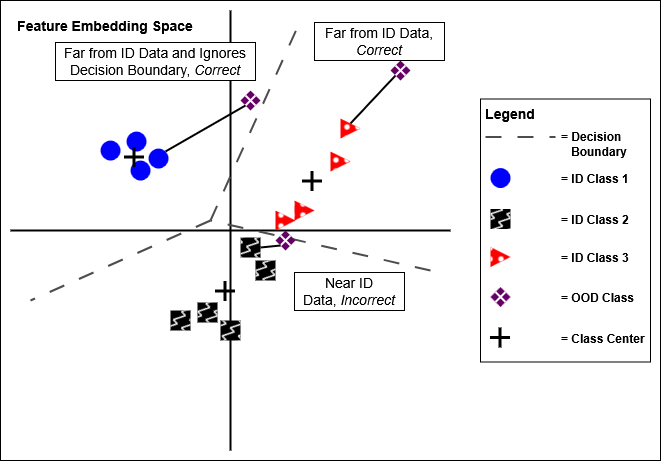
\includegraphics[width=0.9\linewidth]{figures/feats_describe}
  \caption{Example of the functionality of features in detecting ID and OOD test samples. Discriminative features are critical for OOD detection with features, leading to the issue with the lower OOD sample. Despite being near the decision boundary, it was detected as ID because it is close to ID data. Discriminative features would better separate the ID and OOD data in the feature space.
  }
  \label{fig:relwork-feats_example}
\end{figure}

The importance of features in \gls{ood} detection has become a major point of recent discussion in the field. A model's ability to learn \gls{id} class-representative discriminative features significantly influences its ability to distinguish \gls{id} testing data samples from \gls{ood} samples. This is illustrated in \ref{fig:relwork-feats_example}, where \gls{ood} data that lie near \gls{id} data in the feature space are incorrectly detected. Models that learn spurious features, which correlate to \gls{id} classes but do not contribute discriminative meaning, perform worse in \gls{ood} detection \cite{zhang2023openood,salehi2022unified}. Existing works have analyzed components of images, such as the backgrounds in images containing an object, to isolate sources of spurious features and develop mechanisms to prevent learning them \cite{ming2022exploit,neuhaus2023spurious}. The discussion of discriminative and spurious features is closely related to the well-known problem of near- and far-\gls{ood} detection. Specifically, the \gls{ood} detection problem is divided into two subsets according to difficulty in detecting the \gls{ood} samples. Far-\gls{ood} datasets are clearly separable from \gls{id} data, exhibiting severe covariate shift (differing domain from the overall \gls{id} distribution), severe semantic shift (differing features from the \gls{id} classes), or both. Near-\gls{ood} datasets overlap with the \gls{id} data distribution in some capacity, having little to no covariate or semantic shift \cite{yang2022openood,wang2023connecting,winkens2020contrastive,zhang2023openood}. The existence of near-\gls{ood} data is of critical importance in transitioning \gls{ood} detection from clinical environments to applications \cite{salehi2022unified,khazaie2022towards,wu2025out,zhang2021understanding,vaze2022generalized}. Several works have already begun to address the issue of adjusting \gls{ood} detection concepts and methods to realistic settings through adaptations such as improved outlier exposure \cite{azizmalayeri2022your} or robustness \cite{chen2020robust,meinke2022provably}. Despite these efforts, near-\gls{ood} detection remains a present issue in the field with many modern works neglecting to experiment on near-\gls{ood} datasets or struggling to outperform existing baselines \cite{gong2025out,ling2025cadref}. The near-\gls{ood} detection problem, and the related issue of learning discriminative features, exist as the next major challenge to both the field of \gls{ood} detection and the expansion of ML to open-world settings.

\section{Multi-View OOD Detection}
\label{sec:relwork-mvood}

%Multi-view classification \cite{seeland2021multi} has been studied by many researchers  \cite{su2015multi,zhao2023cddfuse} and used in numerous applications \cite{liu2019multi,zhan2023cfnet}. However, few works have leveraged foreground and background views of images \cite{geng2023foreground}.
%Recent progress has been oriented around the use of Transformer-based attention \citep{dosovitskiy2020image} layers \citep{zhao2023cddfuse,chen2021crossvit}. By using self-attention and cross-attention methods \citep{frank2021vision}, class-relevant features in data can be attended to both within and across views \citep{li2023mvhanet}. %Further performance gains were observed with further refinements to view feature fusion \citep{wang2024mutualformer} and alignment of learned features \citep{ke2024rethinking}. 
%Our work is different from cross-attention methods: (1) we leverage complementary information across three views using feature fusion in a novel hierarchical cross-attention and fusion architecture and (2) we uniquely apply this idea to foreground-background view data to improve OOD detection.
Multi-view classification is a field of ML that investigates the use of multiple different views of an images for a classification task. Each view is a distinct image derived from the original image and containing a subset of the features in the original image \cite{seeland2021multi}. Developments in the field have shown the benefits of multi-view learning in different architectures and across various applications \cite{su2015multi,zhao2023cddfuse,liu2019multi,zhan2023cfnet}. Recently, the prevalence of Transformer-based attention \cite{dosovitskiy2020image} has drawn the interest of the multi-view community. Studies have shown that models based on Transformers also benefit from multi-view learning, outperforming previous multi-view baselines (e.g. using convolutional NNs) \cite{zhao2023cddfuse,chen2021crossvit}. Innovations on self-attention and cross-attention methods \cite{frank2021vision} exploit the rich feature information across views \cite{li2023mvhanet} and enable fusion of view features into a more informative embedding for classification and other downstream tasks \cite{wang2024mutualformer,ke2024rethinking}. With respect to the choice of views, previous work primarily uses rudimentary transformations of the original image or different perspectives of the same object \cite{geng2023foreground}.

While multi-view classification has grown as a research field, there has been little-to-no work investigating the intersection between multi-view methods and \gls{ood} detection. Often, related works treat anomalous images (or components of images) as ``\gls{ood}'' and apply basic uncertainty estimation techniques to approximately detect these samples at test-time \cite{fernandez2023out,jung2022uncertainty}. Another work followed the related direction of augmenting images to separate \gls{id} images from anomalous images \cite{radford2021learning}.

%Little work has been done on multi-view OOD detection. One work used multi-view autoencoders to improve lesion detection in prostate cancer MRI images \cite{fernandez2023out}. \citet{jung2022uncertainty} improved OOD detection capabilities of multi-view Gaussian Processes. However, they do not consider deep NNs 
%and their views only vary the level of corruption noise injected into images. Another work uses CLIP \cite{radford2021learning} to identify ID-irrelevant nuisances to improve OOD detection but doesn't consider explicit image background separation or intelligent fusion of view features \cite{miyai2024locoop}. To our knowledge, no existing work has leveraged foreground-background views and feature fusion for OOD detection. An additional review of related work can be found in Appendix Sec. \ref{sec:suppmat-relwork}.
Image segmentation in multi-view contexts has only been sparsely explored. Within the field of \gls{ood} detection, several works have used foreground-segmented images for anomaly detection but they discard the background instead of utilizing it for additional features  \cite{tian2024foct,miyai2024locoop}. One solution used Vision Language Models and prompt learning to extract foregrounds, using \textit{both image and text} as input for few-shot \gls{ood} detection \cite{miyai2024locoop}. These approaches typically neglect full usage of all available image view features (e.g. backgrounds) or leverage other additional data modalities, rendering them incomparable to image-only or text-only \gls{ood} detection methods (which are the subject of this thesis). Another approach disentangles foregrounds and backgrounds in images but uses dense prediction instead of segmentation. It further applies the views to open-world classification instead of \gls{ood} detection \cite{ding2024improving}. Another typical problem exists at the frontier of segmented image-based, multi-view \gls{ood} detection research. Performance is generally poor compared previous single-view state-of-the-art \gls{ood} detection baseline methods. The problem of \gls{ood} detection using segmented images and multi-view methods remains open, with great potential.

\section{OOD Detection with Natural Language}

%In OOD detection, 
%\textit{confidence-based methods} use model logits to quantify confidence in a sample for evaluating its familiarity (i.e., ID or OOD) \cite{yang2024generalized,hendrycks2017baseline,wei2022mitigating,liu2020energy,sun2021react,liu2023gen,hofmannenergy}. Uncertainty estimation and augmented predictions have also been shown to improve logit quality for OOD detection \cite{thulasidasan2019mixup,liu2024fast,huang2021mos,sun2022dice,yu2023block,chen2024optimal,regmi2025adascale}.
%\textit{Self-supervised approaches} focus on learning better features for use in downstream OOD detection tasks \cite{hendrycks2019using}. Such methods include contrastive losses \cite{tack2020csi,ming2022exploit}, generative \cite{wang2022cmg,du2022vos} methods, or data augmentation \cite{zhang2024if,thulasidasan2019mixup, yun2019cutmix, hendrycks2022pixmix}. These methods have been explored in NLP and LLM-based OOD detection in varying capacities \cite{baran2023classical}.
%Domains related to OOD detection have been explored such as uncertainty quantification in LMs \cite{chen2024reconfidencing,ma2025estimating,xiong2023can,ye2024benchmarking}, OOD generalization \cite{wang2024can}, and quality assurance \cite{ouyang2025textual}, but have not been thoroughly applied specificlaly to the OOD detection problem \cite{zhou2023navigating}. 
%In natural language processing (NLP), OOD detection has also been studied \cite{lang2023survey,xu2024large}. Existing methods have shown fine-tuning on ID data to improve LLM OOD detection performance \cite{salimbeni2024beyond,zhang2024your,xu2022contrastive}. Other methods use model features or predicted logits and probabilities to quantify an OOD detection score \cite{lee2024ced,huang2024out,cao2024envisioning,baran2023classical}. However, all of these methods assume access to LLM components and training.
With the advent of large language models (LLMs), the field of natural language processing (NLP) has exploded in popularity. This has naturally nurtured an analogous growth in interest on the performance of such models when exposed to \gls{ood} samples \cite{baran2023classical,lang2023survey,xu2024large,yang2023out}. Related areas including uncertainty quantification \cite{chen2024reconfidencing,ma2025estimating,xiong2024can,ye2024benchmarking}, \gls{ood} generalization \cite{wang2024can}, and quality assurance \cite{ouyang2025textual} have attempted to establish the \gls{ood} detection problem in NLP \cite{zhou2023navigating}. Existing work on \gls{ood} detection in NLP have expanded other problems, such as the text classification task, to encompass identifying and classifying \gls{ood} test data \cite{zheng2020out,toth2024classification,garg2021towards}. More principled approaches consider quantifying the uncertainty in NLP-based methods and models \cite{da2024llm,xiong2024can,tian2023just}, including studying noise in NLP models and data \cite{al2021towards,chen2023automatic} and exposing models to synthetic \gls{ood} samples \cite{li2024conan,kim2023pseudo}.

With respect to LLMs, \gls{ood} detection has become a rapidly growing domain \cite{xu2025large,liu2024good,wang2024can,liu2024can,sali2025navigating,zaera2025efficient}. Initial work investigated fine-tuning to improve LLM characterization of the \gls{id} decision boundary and detection of \gls{ood} samples \cite{salimbeni2024beyond,zhang2024your,xu2022contrastive,hanparameter,kim2024investigation,wang2025chain,singh2025few,castillo2025intent}. Another direction of works instead focuses on improving and extracting LLM features or logits for \gls{ood} detection scoring \cite{lee2024ced,huang2024out,cao2024envisioning,baran2023classical,uppaal2023fine,tint2025prood}. In a set of works that draw from self-supervised learning, negative (i.e. synthetic alternative) classes or text domains were shown to be beneficial in augmenting LLMs for \gls{ood} detection \cite{huang2024out,luo2025semi}. Following from work in outlier exposure, success has likewise been observed in exposing LLMs to \gls{ood} data during training to improve \gls{id} and \gls{ood} separation at test time \cite{cao2024envisioning,park2023powerfulness,xu2023contrastive}. \gls{ood} detection in LLMs has also been considered as part of the design principles in many state-of-the-art foundation models. The inclusion of mixture-of-experts components in LLMs improves learning of discriminative \gls{id} knowledge, in turn improving uncertainty awareness during generation \cite{dai2024deepseekmoe,jiang2024mixtral}. Recent advances in agentic models have incited similar discussions on evaluating uncertainty awareness and improving \gls{ood} detection \cite{lee2025concept}. 

Of note is the recent focus of \gls{ood} detection on leveraging images and text, particularly in the form of Vision Language Models (VLMs) \cite{miyaigeneralized,lee2025harnessing,dai2023exploring,alnegheimish2025m}. Traditional methods, such as fine-tuning VLMs for \gls{ood} detection \cite{zeng2024local,xu2025overcoming}, have demonstrated clear effectiveness in solving the task. However, explorations into improving alignment between learned text and image embeddings suggests significantly greater depth in the multi-modal domain \cite{kim2025enhanced,zhang2025runa}. A greater interest in few-shot and zero-shot \gls{ood} detection has also developed recently, in which models must separate \gls{id} and \gls{ood} samples with either little-to-no \gls{id} training or no access to \gls{id} training samples at all \cite{madan2024revisiting,esmaeilpour2022zero}. 

\subsection{Prompting and OOD Detection}

One of the fundamental components in LLMs is the prompt, which contextualizes the task provided to the model and acts as the conditional distribution over which inference operates \cite{mei2025survey}. An expansive and rich history of investigations into prompts has resulted in a deep understanding on methods which improve LLM performance across a breadth of tasks. \textit{Reasoning} stands as a major prompting refinement (or equivalently, prompt engineering) method that encourages model refinement of knowledge \cite{munkhbat2025self,agarwal2023kitlm,zhou2022least,huang2023language,zhang2022automatic,shi2022language}. This can take multiple forms, including cognitive reasoning \cite{kramer2024unlocking} which aims to dissect LLM reasoning into a procedure of reasoning tools, or self-refinement \cite{madaan2023self,shinn2023reflexion,zhou2024isr} in which the LLM iterates over outputs until a consistent response is generated. Inclusion of examples within prompts, an example set of techniques being \gls{icl}, has been discovered to be extremely effective in many tasks \cite{dong2024survey}. Agentic prompting, resulting from the aforementioned increase in agentic LLM investigations, also shows promise in improving model efficacy \cite{yue2024fragrel,chen2022program}.

%Recently, a prompt-based method to OOD detection using LLMs was proposed. It does not have access to model features, logits, or fine-tuning. To our knowledge, \citep{wang2024beyond} is the sole study in this direction, using only prompts and detection of LLM response of ``unknown'' or a predicted intent to perform OOD detection. Specifically, a verbal prompt was used to provide the LLM with examples from ID classes and the input query before requesting the model to provide the corresponding ID class of the input or ``unknown'' if no ID class was relevant. The LLM output was parsed to identify if the correct class was generated for ID test samples or ``unknown'' was generated for OOD samples. We follow this direction and demonstrate that using more intelligent reasoning from the LLM, state-of-the-art prompt-only OOD detection can be achieved by converting existing OOD detection techniques into a prompt.
With respect to \gls{ood} detection, nearly all works in NLP- and LLM-based \gls{ood} detection assume access to model components (features and logits) or \gls{ood} data. The sparse domain of \textbf{prompt-only \gls{ood} detection} shows great promise in applications, functioning without unrealistic assumptions while improving model detection performance and increasing accessibility for users. Existing works are extraordinarily limited, with one work proposing the idea solely through generation of ``unknown'' or an \gls{id} class for detection \cite{wang2024beyond}. Prompt-only \gls{ood} detection exists as a task rich with potential for future innovation and application. In particular, the concept of \textit{alignment} \cite{yousef2020survey,wang2020measurement,bani2025hybrid,zaricna2015word,yang2019simple,chang2021deep,xylogiannopoulos2025power} has been thoroughly studied but has yet to be applied to \gls{ood} detection. Specifically, the notions of lexical alignment \cite{el2021xlent,dyer2013simple,srivastava2025measuring} and semantic alignment \cite{el2021xlent,thompson2020cultural} exhibit potential for use in \gls{ood} detection via prompting of LLM reasoning and generation of OOD scores.

%We evaluated their method both in the open-set classification setting and the OOD detection setting, and showed that in both cases the approach was suboptimal. Instead, we show that leveraging alignment with LLM reasoning and thesholding of OOD scores greatly improves performance and, interestingly, can even outperform feature- and logits-based OOD detection methods. We induce alignment through prompting of an LLM and find the utilization of both lexical alignment \citep{el2021xlent,dyer2013simple,srivastava2025measuring} and semantic alignment \citep{el2021xlent,thompson2020cultural} to be beneficial. Previous work on alignment manually defines alignment metrics and do not consider ICL. %, while we induce alignment in the generation of an LLM.
% new refs: to organize/add
% bani2025hybrid - alignment
% zaricna2015word - alignment
% yang2019simple - alignment
% yousef2020survey - alignment [survey]
% chang2021deep- alignment
% xylogiannopoulos2025power - alignment
% bhavana2024plagiarism - alignment (plagiarism)
% wang2020measurement - alignment [survey]
% sajid2025comparative - alignment (plagiarism)
% vrbanec2017struggle - alignment (plagiarism)
% chen2021empirical - MOCOv3
% oquab2023dinov2 - DINOv2
% caron2020unsupervised - SWAV

% TODO add below to nlp/llm section
%\vspace{2mm}
%\section{Related Work}
%OOD detection is a well-studied area with many effective techniques %solution to the open-world problem setting of ML 
%\citep{ghassemi2022comprehensive, zhang2023openood}.
%%OOD detection has been investigated from many different directions. 
%%Distance-based methods use a measure of distances, often in the model feature space, to detect OOD samples. Examples include Mahalanobis distance \cite{lee2018simple,ren2021simple}, %which uses covariance to estimate sample distance from ID data, 
%%non-linear space comparisons between samples \cite{sun2022out,regmi2024reweightood,ahn2023line}, and combined distance measurements between decomposed subspaces with logits-based confidence scores \cite{wang2022vim,ammar2024neco}.
%Logits-based methods use model predictions to estimate uncertainty in OOD samples \citep{hendrycks2019scaling}. Feature-based methods use measures of distance in the feature space, such as Mahalanobis distance \citep{lee2018simple,ren2021simple}, non-linear comparisons \citep{sun2022out,regmi2024reweightood}, and hybrid metrics \citep{wang2022vim,ammar2024neco}, to detect OOD samples.
%
%% llm
%% X - wang2024beyond (llm ood intent detect)
%% - liu2024good (llm ood detect)
%% X - wang2024can (icl ood generalization)
%% - liu2024can (ood detect from foundation models)
%% - dong2022survey (icl - survey)
%% X - lang2023survey (nlp ood detect - survey)
%% - zheng2020out (nlp ood detect - old, moderate citation count)
%% X - baran2023classical (ood detect* - classic methods w/ nlp models including llms)
%% X - chen2024reconfidencing (llm uncertainty - icl)
%% X - ma2025estimating (llm uncertainty)
%% X - xiong2023can (big llm uncertainty paper benchmark)
%% X - ye2024benchmarking (llm uncertainty benchmark)
%% X - lee2024ced (nlp ood detect - feats)
%%  + sample perturb is viable
%% - ouyang2025textual (nlp ood detect)
%% X - salimbeni2024beyond (llm ood detect - fine tuning)
%% X - zhang2024your (llm ood detect - fine tuning)
%% X - xu2024large (llm ood detect - survey)
%% X - huang2024out (llm ood detect - feats, vlm)
%% X - cao2024envisioning (llm ood detect - feats, vlm)
%% X - xu2022contrastive (llm ood detect - reqs separate trained model)
%% X - zhou2023navigating (llm uncertainty - it's unreliable)
%% *re-read and follow progression from nlp ood survey
%% singh2025few (need to train generative flow network, open-set classification)
%% castillo2025intent (fine-tuned LM + another LLM, open-set classification)
%% sali2025navigating (trained sentence transformer + another LLM, also open-set classification)
%% zaera2025efficient (trained LM, clustering required, fine-tuned LLM, also open-set classification)
%% tint2025prood (feature-based)
%% chow2025prompt (uses training for OOD detection)
%
%\textbf{Prompt-Only OOD Detection with LLMs.} 
%Recently, \citet{wang2024beyond} proposed a prompt-only ($C$+1)-classification method using LLMs, assuming no access to model features or logits. It addresses the OOD detection task tangentially but is the \textbf{only} previous work that considers prompt-only OOD detection.
%Specifically, it prompts an LLM with ID class examples and the input query before model output is parsed for either an ID class or ``unknown'' (OOD) if no ID class was relevant. 
%
%% The LLM output was parsed to identify if the correct class was generated for ID test samples or ``unknown'' was generated for OOD samples. 
%%To our knowledge, it is the sole study in this direction. However, our experiments show that our \sys outperforms this method. %We advance this direction by proposing to convert existing OOD detection methods into a prompt. % demonstrate that using more intelligent reasoning from the LLM, state-of-the-art prompt-only OOD detection can be achieved by 
%%It converts an existing OOD detection technique into a prompt.
%More related work is in Appendix Section 3.
\chapter{Preliminary Investigations into Multi-View OOD Detection}
\label{diss_mvood_init}

%\textcolor{red}{NOTE: I think most of the results and code for this section are from the ACER server so they are stored in the /hdd_1/politow2/ACER_bkp/experiments/MEO.zip and smv_ood.zip files. I think\dots}

%(mv cnn definitions etc.)
%(establish mathematical definitions and explain toolkit/procedure used in detail)

\section{Multi-View OOD Detection Frameworks}
\label{sec:m1-mvcnns}

%The incorporation of multi-view data in OOD detection models is established by using 1) an off-the-shelf image segmentation tool and 2) a multi-view ML model pipeline. First, an image $x$ is segmented into two ``views'': its foreground ($x_{fg}$) and background ($x_{bg}$) view. A specific image segmentation tool (IST) for performing the segmentation is detailed in Section \ref{sec:propwork-mod-exp}. The segmentation operation results in a set of foreground object pixels in $x$ which is used as the foreground view $x_{fg}$. The background view $x_{bg}$ is the negative mask of the foreground object pixels. The original image $x$, which henceforth is equivalently denoted as the original view $x_{org}$, is included with the foreground view $x_{fg}$ and the background view $x_{bg}$ to create the resultant multi-view set for given sample image $x$ after the segmentation step, \{$x_{org}$, $x_{fg}$, $x_{bg}$\}. For convenience, the set of views is denoted as $V = \{org, fg, bg\}$ and is comprised of each individual view $v \in V$. In practice, the multiple views for any given dataset can be generated offline prior to use in training or OOD detection testing to improve efficiency. 
%A multi-view dataset $\mathcal{D}_{MV} = \{(x_{MV,i}, y_i)\}$ contains set of labels $y_i$ and a set of associated multi-view samples $x_{MV,i}$. Each multi-view sample is composed of a set of \emph{views} $x_{MV,i} = \{x_{i,0}, x_{i,1}, \dots, x_{i,V}\}$ where $V$ is the number of views. Views are images, with each view being a copy of the original image under covariate or semantic shift (including no shift, i.e. the original image itself). That is, given some augmentation function introducing covariate or semantic shift $\mathcal{A}(\cdot)$, a view is defines as $x_{i,v} = \mathcal{A}(x_i)$ for original image $x_i$ and with $v \in \mathbb{N}^V$.
The challenge in image-based \gls{ood} detection has predominantly shifted to solving the problem of detecting near-\gls{ood} data \cite{yang2022openood,winkens2020contrastive}. As previously mentioned, near-\gls{ood} is considered to be \gls{ood} data that has significant covariate and/or semantic overlap with the \gls{id} data distribution. Detection of near-\gls{ood} data relies on model learning of discriminative features representative of \gls{id} data (or classes) and subsequent rejection of spurious features \cite{ming2022impact,neuhaus2023spurious}. Existing multi-view and \gls{ood} detection works primarily focus on \emph{augmenting} data through various transformations that serve to increase the diversity of data in the \gls{id} distribution and improve model learning \cite{shorten2019survey,hendrycks2022pixmix,geng2023foreground}. However, studies investigating the behaviors of ML models and the impact of spurious features on learning have revealed patterns identifying foregrounds and backgrounds of images as critical components separating discriminative and spurious features \cite{geng2023foreground,miyai2024locoop}. There has been very little work in the multi-view literature that considers this approach to multi-view learning, i.e. using foregrounds and backgrounds as views, emphasizing the need for investigation in this direction of research. It is hypothesized that using foregrounds and backgrounds of an image as views can improve model learning of discriminative features in images, thus improving \gls{ood} detection and particularly advancing the field in performance on challenging near-\gls{ood} detection settings. This also pushes ML closer to realistic deployment in open-world settings, of interest in many applications (see Chapter \ref{diss_intro}). The hypothesis is supported by observations in medical research, positing that segmentation is a critical function in rapid object identification in humans \cite{weiner2016anatomical,vuilleumier2002multiple}.

A foreground-background multi-view \gls{ood} detection method involves a pipeline containing two components: 1) a foreground-background (FgBg) \gls{ist} $f_{IST}$, and 2) a multi-view model $f_{MV}$. FgBg segmentation is an operation $\mathcal{K}$ that takes as input an image $x$ and outputs a set of foreground pixels which is used as the foreground view $x_{fg}$. That is, given that $x$ is an image, $x_{fg} = \{(\text{pixel},i,j) | (i,j) \in \mathcal{K}(x)\}$. The background view $x_{bg}$ is the result of using the foreground pixels as a negative mask on the original image $x$, $x_{bg} = x \setminus x_{fg}$. Note that here the set definitions with $\mathcal{K}$ are the result of the aforementioned view-generating augmentation function $\mathcal{B}$ mentioned in previous multi-view work (see Chapter \ref{diss_bkgd} Section \ref{sec:bkgd-mvp}). Multi-view samples are then constructed using the original image, henceforth referred to as the original view $x_{org}$, and the foreground and background views $x_{MV} = \{x_{org}, x_{fg}, x_{bg}\}$. A shorthand is introduced here denoting the set of views as $V = \{org, fg, bg\}$, comprised of each individual view $v\in V$. In practice, the FgBg views for any dataset are generated offline with the \gls{ist} prior to use in training or testing for convenience. %Analysis is provided later (see Section \ref{}) for evaluation of method complexities and relevant resource consumption of all components involved in proposed methods.

%Second, each of the three views is processed using a multi-view image processing ML model. For the subsequent proposed works, the model is a multi-view convolutional NN (CNN), or MVCNN \cite{su2015multi}. An MVCNN is composed of a set of CNN feature extractors $\Phi_{V} = \{\phi_{org}, \phi_{fg}, \phi_{bg}\}$, one for each input view $v \in V$, and a fusion module $\mathcal{G}$. The CNN feature extractors are responsible for coalescing input image data into a feature vector representative of class-relevant image information, while the fusion module is responsible for regulating how much information should be included in the final model feature vector from each of its input view feature vectors. A CNN feature extractor $\phi_{v}$ takes as input its corresponding view $x_{v}$ and outputs a $p$-dimensional feature vector $z_{v} \in \mathbb{R}^{p}$, $\phi_{v}: \mathcal{X} \mapsto \mathbb{R}^{p}$. The CNN feature extractors $\Phi_{V}$ output a set of \textbf{view-specific} feature vectors \{$z_{org}$, $z_{fg}$, $z_{bg}$\} which are then passed to a fusion module $\mathcal{G}$. A fusion module $\mathcal{G}$ takes as input feature vectors from each view $v$ and outputs a combination of feature $Z_{mv}$ and prediction logits $\hat{Y}_{mv}$. %\textcolor{blue}{do we need more detail on fusion module and in general here?} 
%Details on the MVCNNs and fusion modules used in the presented works for OOD detection are provided in Sections \ref{sec:propwork-mod-propmeth} and \ref{sec:propwork-meo-propmeth}. An example of such a pipeline is given in Figure \ref{fig:propwork-mod-diagram}. %\textcolor{blue}{maybe add some sentences here walking through the diagram and matching key features to described components}
%Multi-view models process multi-view datasets by taking each view in a multi-view sample as input and calculating some representative representation coalescing information across the views as output. The multi-view model $f_{MV}$ may be considered as a set of individual-view models $f_{MV} = \{f_0, f_1, \dots, f_V\}$. Each view in a multi-view sample $x_{i,v}$ is processed by its corresponding individual-view model $f_v$. Note that each individual-view model can be the same, and thus shared. Outputs from each individual-view model are then coalesced in an operation referred to as ``fusion'', resulting in a collective output from the multi-view model $f_{MV}(x_{MV,i}) = \mathcal{U}(\{f_0(x_{i,0}),f_1(x_{i,1}),\dots,f_V(x_{i,V})\})$ for fusion operation $\mathcal{U}$.
FgBg multi-view models are composed of a set of image processing models and a fusion component handling the fusion operation (these terms will be used interchangeably), $\mathcal{U}$. The image processing models can be decomposed into several sets, each of which is equivalent to a full image processing model. Specifically, individual view model $f_v$ is decomposed into a feature extractor $\phi_v$ and a classification layer weight matrix $W_v$ with optional bias $b_v$. Thus, the multi-view model becomes a decomposed multi-view feature extractor set $\phi_{MV} = \{\phi_v | v \in V\}$, multi-view classification weight matrix set $W_{MV} = \{W_v | v \in V\}$, and optional multi-view classification bias set $b_{MV} = \{b_v | v \in V\}$. Individual view features $z_v = \phi_v(x)$ and predicted logits $\hat{y}_v = W_v z_v + b_v$ are represented by the multi-view sets $Z_{MV} = \{z_v | v \in V\}$ and $\hat{Y}_{MV} = \{\hat{y}_v | v \in V\}$. The fusion component $\mathcal{U}$ outputs a fused feature $z_{\mathcal{U}}$ and fused predicted logits $\hat{y}_{\mathcal{U}} = W_{\mathcal{U}} z_{\mathcal{U}} + b_{\mathcal{U}}$ for fused classification weight matrix $W_{\mathcal{U}}$ and optional bias $b_{\mathcal{U}}$.

%Of note is that using multiple views of data \emph{is not equivalent} to using additional training data. Instead, multi-view data is a sophisticated utilization of given data specifically targeted towards learning and exploiting salient discriminative features in image data. In this case, segmentation into foreground and background views can be seen as parallel to data augmentation, exposing models to additional information using a more diverse set of images. However, the proposed method does not add additional information to any given data sample, instead only enabling better separation of information. In all presented evaluations, the same training and test datasets are used to train and evaluate the proposed methods as are used by the compared baselines.}
Of note is that using multi-view data is \textit{not equivalent} to simply using additional training data. The views $x_{MV}$ resulting from augmentations on any given input $x$ provide covariate and/or semantic information highly correlated \textit{with respect to} the original sample. As such, processing views in a multi-view framework exploits this contextual correlation while additional data foregoes this in favor of naive learning. This approach, that is of using additional data, has been shown theoretically to be insufficient in solving the \gls{ood} detection problem \cite{fang2022out}. It is further demonstrated in this dissertation that multi-view processing is necessary to exploit $x_{MV}$ for improved OOD detection (see Sections \ref{sec:propwork-mod-exp}, \ref{sec:propwork-meo-exp}, \ref{sec:propwork-scod-exp}, and Chapter \ref{diss_casod} Section \ref{sec:propwork-casod-exp}).

\section{View Selection for OOD Detection}
\label{sec:propwork-mod}

%(motivation: not all views provide reasonable features, maybe we can only fuse useful views)

%The purpose of foreground-background segmentation-based views is to separate class-relevant discriminative features from potential misleading spurious features. In order to avoid spurious views, the proposed method, \textbf{M}ulti-view \textbf{O}oD \textbf{D}etection (\textbf{\sysa}), introduces a \textbf{view selector} to the fusion module in an MVCNN model . This view selector explicitly considers the discriminative features %necessary for OOD detection 
%in the foreground and background views before selecting one and using only that view for feature fusion with the original view (which is always used). The view selector is trained with a loss favoring whichever view is making more accurate predictions, based on the reasoning that a better-performing view must be extracting more meaningful semantic information with respect to ID classes. This strategy simultaneously biases the fusion module away from the misleading view and towards the view with more class-relevant discriminative features. The entire pipeline of processing multi-view data and learning the view selector is designed to be fully learnable and autonomous. %\textcolor{blue}{do we want to move the name of the method to a more strategic location instead of the first mention of it?}
Following from existing literature investigating spurious features in the context of \gls{ood} detection, the segmented view containing the \gls{id} object contains discriminative features representative of \gls{id} class objects while the remaining view likely contains primarily spurious features \cite{miyai2024locoop,neuhaus2023spurious}. In the proposed FgBg multi-view domain, the view containing discriminative or spurious features depends on the \gls{ist}. For example, an \gls{id} class of ``dog'' is clearly segmented with discriminative features in the foreground view while an \gls{id} class of ``mountain'' is segmented with discriminative features predominantly in the background (see \ref{fig:intro-mvexample}). In \gls{ood} detection, it is desired to only consider the \gls{id}-class representative discriminative features for optimal learning and separation of \gls{id} and \gls{ood} samples. Following from the previous example, if the model could automatically identify the foreground as the relevant view for the ``dog'' sample (and the background for the ``mountain'' sample), then an improved awareness of \gls{id} features would be learned and \gls{ood} data would be detected with greater accuracy.

To facilitate this idea, the proposed method, %\textbf{M}ulti-view \textbf{O}OD \textbf{D}etection (\textbf{\sysa})
\gls{sysa}, considers the novel use of a \textbf{view selector} as the fusion component in an FgBg multi-view \gls{ood} detection model. The view selector evaluates the discriminative features in the foreground and background views, selecting the superior view for fusion with the original view (which is always used, as it contains full feature information for the sample). Using a novel loss function, the view selector is trained to bias the view which has greater \gls{id} class prediction accuracy, following the assumption that increased classification performance correlates with learning of more meaningful semantic features. By leveraging this view selection mechanism, the model simultaneously rejects the view with spurious features and incorporates the additional, correlated discriminative information in the selected view.

\subsection{Proposed Method}
\label{sec:propwork-mod-propmeth}

%(proposed architecture with explanation)

%Second, each of the three views is processed using a multi-view image processing ML model. For the subsequent proposed works, the model is a multi-view convolutional NN (CNN), or MVCNN \cite{su2015multi}. An MVCNN is composed of a set of CNN feature extractors $\Phi_{V} = \{\phi_{org}, \phi_{fg}, \phi_{bg}\}$, one for each input view $v \in V$, and a fusion module $\mathcal{G}$. The CNN feature extractors are responsible for coalescing input image data into a feature vector representative of class-relevant image information, while the fusion module is responsible for regulating how much information should be included in the final model feature vector from each of its input view feature vectors. A CNN feature extractor $\phi_{v}$ takes as input its corresponding view $x_{v}$ and outputs a $p$-dimensional feature vector $z_{v} \in \mathbb{R}^{p}$, $\phi_{v}: \mathcal{X} \mapsto \mathbb{R}^{p}$. The CNN feature extractors $\Phi_{V}$ output a set of \textbf{view-specific} feature vectors \{$z_{org}$, $z_{fg}$, $z_{bg}$\} which are then passed to a fusion module $\mathcal{G}$. A fusion module $\mathcal{G}$ takes as input feature vectors from each view $v$ and outputs a combination of feature $Z_{mv}$ and prediction logits $\hat{Y}_{mv}$. %\textcolor{blue}{do we need more detail on fusion module and in general here?} 
For \gls{sysa}, the FgBg multi-view model $f_{MV}$ is implemented using a convolutional neural network (CNN) capable of processing multiple views, or \gls{mvcnn} \cite{su2015multi}, as the backbone. The multi-view feature extractors are each a CNN feature extraction backbone parameterized by $\theta$, $\phi_v = f_{\theta,v}$. Each $f_{\theta,v}$ learn view feature vectors representative of \gls{id} class information, taking as input the corresponding view $x_v$ and outputting a $d$-dimensional feature vector $z_v \in \mathbb{R}^d$, $\phi_v: \mathcal{X} \mapsto \mathbb{R}^d$. Here, $V = \{org, fg, bg\}$, and the multi-view feature extractors $\phi_{MV}$ give $Z_{MV} = \{z_{org}, z_{fg}, z_{bg}\}$. The corresponding individual classification weight matrices $W_{MV}$ and biases $b_{MV}$ give $\hat{Y}_{MV} = \{\hat{y}_{org}, \hat{y}_{fg}, \hat{y}_{bg}\}$. In \gls{sysa}, the fusion component $\mathcal{U}$ is designed with a view selector, described below, and outputs $z_{\mathcal{U}}$ and $\hat{y}_{\mathcal{U}}$.

\begin{figure}
 \centering
 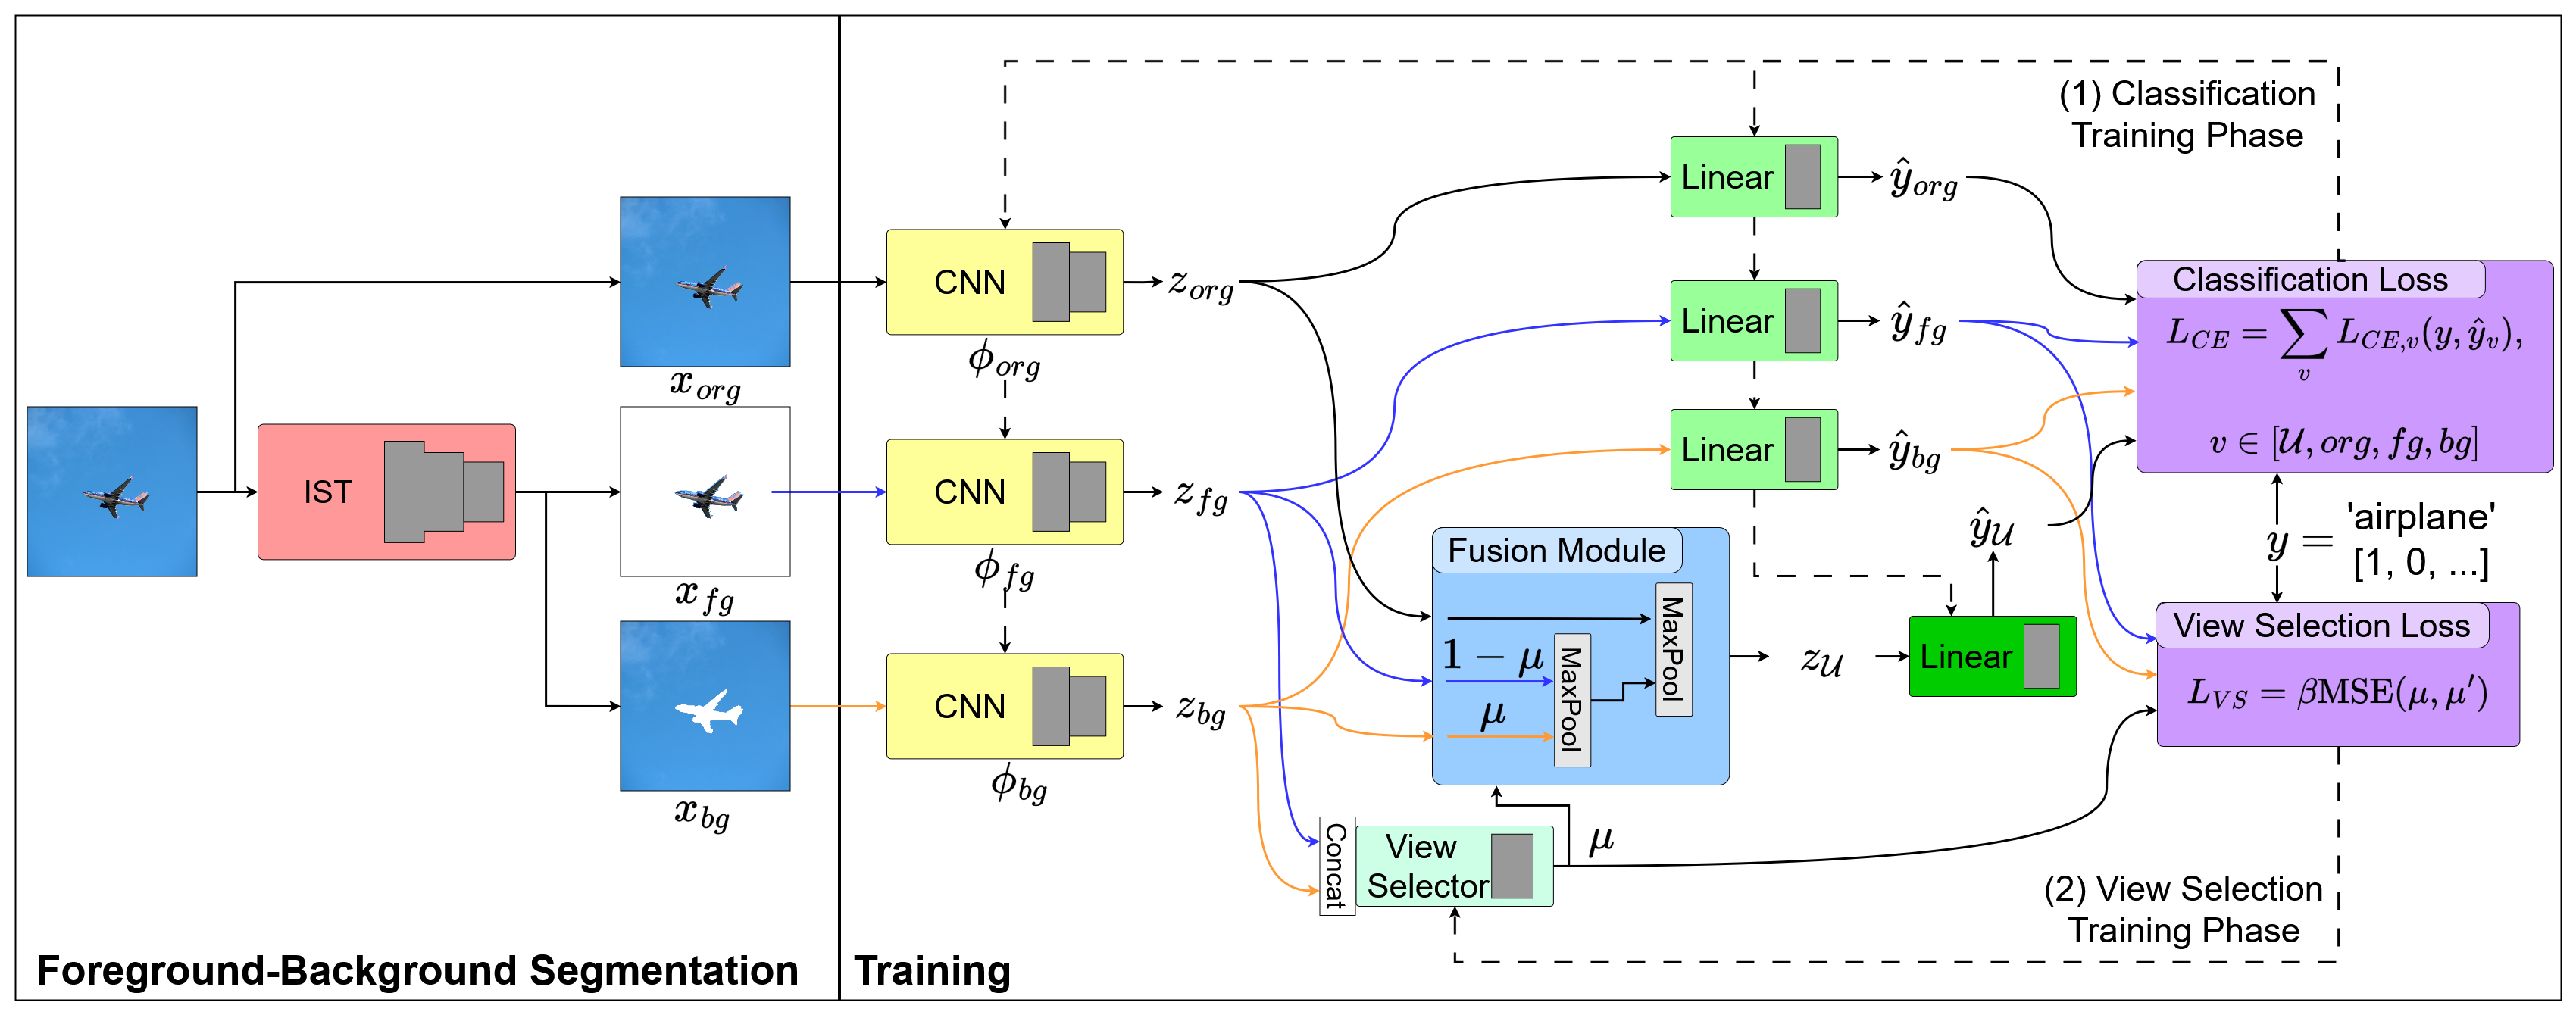
\includegraphics[width=1.\linewidth]{figures/mod_diagram}

  \caption{System diagram of the proposed \sysa. 
  Images are first foreground-background segmented using the IST before being passed to the MVCNN for processing. Note that image segmentation can be done on entire datasets as a setup step.
  Solid lines refer to forward pass, dashed lines refer to backward pass. Black lines refer to the original or fused image features. Blue lines refer to foreground image features, orange lines refer to background image features. Best viewed in color.
  }
  \label{fig:propwork-mod-diagram}
\end{figure}

%Figure \ref{fig:propwork-mod-diagram} shows the information flow of \sysa. \sysa uses an MVCNN architecture with three view inputs corresponding to the original image view (\textit{org}), the foreground view (\textit{fg}), and the background view (\textit{bg}). Each view $v \in \{org, fg, bg\}$ is passed to its corresponding view feature extractor $\phi_{v}$ resulting in three view-specific feature vectors $z_{org}$, $z_{fg}$, and $z_{bg}$. In this work, the CNN feature extractors $\Phi_{V}$ are implemented using three separate ResNet-18 \cite{he2016deep} models, although this design is modular and any model capable of taking an image as input and generating a feature vector is usable. The three view-specific feature vectors are then passed to the feature fusion module $\mathcal{G}$ which combines the three feature vectors into a fused feature vector $z_{fused} = \mathcal{G}(z_{org}, z_{fg}, z_{bg}) \in \mathbb{R}^{p}$. To enable the model to make more intelligent decisions during fusion, a \emph{view selector} is introduced that determines how much of $z_{fg}$ and $z_{bg}$ to include while producing $z_{fused}$.
The diagram in \ref{fig:propwork-mod-diagram} illustrates the high-level operations and flow of information in \gls{sysa}. An \gls{ist} segments an image into a foreground view and a background view. The \gls{mvcnn} architecture converts the input original image view (\textit{org}), foreground view (\textit{fg}), and background view (\textit{bg}) to view-specific feature vectors $Z_{MV} = \{z_{org}, z_{fg}, z_{bg}\}$. Each feature extractor $\phi_v$ in \gls{sysa} is implemented with a ResNet-18 \cite{he2016deep} model. Of note, however, is that the design of \gls{sysa} is modular. Any model capable of processing an input image and outputting a feature vector $z_v \in \mathbb{R}^d$ is compatible. The fusion component in \sysa $\mathcal{U}_{\text{\sysa}}$ uses \emph{view selection} to combine information in $Z_{MV}$ into a fused feature vector $z_{\mathcal{U}} = \mathcal{U}_{\text{\sysa}}(Z_{MV})$, $z_{\mathcal{U}} \in \mathbb{R}^d$.

%\textbf{View Selector:} The view selector is implemented via a fully connected linear layer $f$ that takes as input the concatenation of the foreground and background view-specific features $[z_{fg}; z_{bg}] \in \mathbb{R}^{2p}$. The output of the view selector is a view selection weight s
%\begin{equation}
%\begin{aligned}
%    s = \sigma(f([z_{fg}; z_{bg}]))
%\end{aligned}
%\end{equation}
%where $\sigma$ is the sigmoid function. Note that the view selector is class-agnostic.
\subsubsection{View Selector}
A critical operation in the proposed fusion component is \emph{view selection}. The view selector is implemented with a fully connected linear layer, represented by weight matrix $W_{vs}$ and bias $b_{vs}$. The foreground and background view-specific feature vectors are concatenated and used as inputs to the view selector, $[z_{fg}; z_{bg}] \in \mathbb{R}^{2d}$, where $[\cdot ; \cdot]$ represents the concatenation operation. The output is a view selection weight $\mu$
\begin{equation}
\begin{aligned}
    \mu = \sigma(W_{vs} [z_{fg}; z_{bg}] + b_{vs}),
\end{aligned}
\end{equation}
where $\sigma$ is the sigmoid function. The view selector is class-agnostic, it evaluates views based solely on the input features.

%\textbf{Fusion Module:} The view selection weight $s$ is used to weight $z_{fg}$ and $z_{bg}$ and perform max-pooling over the weighted view-specific feature vectors, resulting in a weighted foreground-background feature vector $z_{fb}$
%\begin{equation}
%\begin{aligned}
%    z_{fb} = \text{MaxPooling}_{p} \{(1-s) \cdot z_{fg}, s \cdot z_{bg}\}
%\end{aligned}
%\end{equation}
%where $\text{MaxPooling}_{p}$ is a max-pooling operation along each component in the feature dimension $p$. The fusion module $\mathcal{G}$ producing the fused feature vector $z_{fused}$ uses a final max-pooling operation over the original view-specific feature $z_{org}$ and the weighted foreground-background feature vector $z_{fb}$
%\begin{equation}
%\begin{aligned}
%    \mathcal{G}(z_{org}, z_{fg}, z_{bg}, s) = \text{MaxPooling}_{p} \{z_{org}, z_{fb}\}
%\end{aligned}
%\end{equation}
%The final fused feature vector $z_{fused}$ is the resultant output of the fusion module $\mathcal{G}$, $z_{fused} = \mathcal{G}(z_{org}, z_{fg}, z_{bg}, s)$.
\subsubsection{Fusion Component}
The fusion component $\mathcal{U}_{\text{\sysa}}$ for \gls{sysa} utilizes the view selection operation and the view features to selectively combine only the view-specific feature vectors with the most discriminative information. Specifically, the view selection weight $\mu$ weights $z_{fg}$ and $z_{bg}$ before max-pooling is performed over the weighted view-specific feature vectors. The resultant output is a weighted foreground-background feature vector $z_{fb}$
\begin{equation}
\begin{aligned}
    z_{fb} = \text{MaxPooling}_{d} \{(1-\mu) \cdot z_{fg}, \mu \cdot z_{bg}\}.
\end{aligned}
\end{equation}
$\text{MaxPooling}_{d}$ is a max-pooling operation along the feature dimension $d$. The fusion component $\mathcal{U}_{\text{\sysa}}$ outputs a fused feature vector $z_{\mathcal{U}}$, using a final max-pooling operation over the original view-specific feature $z_{org}$ and $z_{fb}$
\begin{equation}
\begin{aligned}
    z_{\mathcal{U}} = \mathcal{U}_{\text{\sysa}}(z_{org}, z_{fg}, z_{bg}, \mu) = \text{MaxPooling}_{d} \{z_{org}, z_{fb}\}.
\end{aligned}
\end{equation}

%\textbf{Prediction:} Prediction logits are produced by feeding each of the generated feature vectors, i.e. $z_{fused}$, $z_{org}$, $z_{fg}$, and $z_{bg}$, to corresponding linear layers, resulting in a fused prediction logits $\hat{y}_{fused}$ and three view-specific prediction logits $\hat{y}_{org}$, $\hat{y}_{fg}$, and $\hat{y}_{bg}$. In the proposed work experiments, only the fused prediction logits is used for ID classification, as the view-specific prediction logits are learned from limited semantic information. In summary, the final outputs of the \sysa fusion module $\mathcal{G}$ are the fused and view-specific feature vectors $Z_{mv} = \{z_{fused}, z_{org}, z_{fg}, z_{bg}\}$ and the fused and view-specific prediction logits $\hat{Y}_{mv} = \{\hat{y}_{fused}, \hat{y}_{org}, \hat{y}_{fg}, \hat{y}_{bg}\}$.
\subsubsection{Prediction}
\gls{sysa} produces logits for each of the view-specific feature vectors $Z_{MV}$ and for the fused feature vector $z_{\mathcal{U}}$. Specifically, each view-specific feature vectors in $Z_{MV}$ is passed through a corresponding linear layer, parameterized by $W_{MV}$ and $b_{MV}$, resulting in view-specific logits $\hat{Y}_{MV}$. The fused feature vector $z_{\mathcal{U}}$ is passed through a fusion linear layer with weight matrix $W_{\mathcal{U}}$ and bias $b_{\mathcal{U}}$, resulting in fused logits $\hat{y}_{\mathcal{U}}$. In \gls{sysa}, only $\hat{y}_{\mathcal{U}}$ is used for \gls{id} classification. As the fused logits learn from all correlated feature knowledge across views, they contain more \gls{id} class-relevant discriminative information for prediction. In contrast, each view-specific logits learns from (and predicts based on) limited feature information.

%\textbf{Training:} \sysa is trained using two alternating losses: a cross-entropy (CE) loss $\mathcal{L}_{CE}$ and a view selection loss $\mathcal{L}_{VS}$.
%
%$\mathcal{L}_{CE}$ is the sum of all fused and individual view CE losses. Specifically, for each view $v \in \{org, fg, bg\}$, a view-specific CE loss $\mathcal{L}_{CE,v}$ is defined as
%\begin{equation}
%\begin{aligned}
%    \mathcal{L}_{CE,v}(y, \hat{y}_{v}) = - \sum_{c \in \mathcal{Y}} y_{c} \log (\hat{y}_{v,c})
%\end{aligned}
%\end{equation}
%where $\hat{y}_{v,c}$ is the logit value of $\hat{y}_{v}$ for class $c$ and $y$ is the one-hot true label vector. The fused prediction logit CE loss $\mathcal{L}_{CE,fused}$ is defined as
%\begin{equation}
%\begin{aligned}
%    \mathcal{L}_{CE,fused}(y, \hat{y}_{fused}) = - \sum_{c \in \mathcal{Y}} y_{c} \log (\hat{y}_{fused,c})
%\end{aligned}
%\end{equation}
%where $\hat{y}_{fused,c}$ is the logit value of $\hat{y}_{fused}$ for class $c$. The final CE loss $\mathcal{L}_{CE}$ is the sum of the four losses
%\begin{equation}
%\begin{aligned}
%    \mathcal{L}_{CE} = \smashoperator{\sum_{v \in \{fused, ~org, ~fg, ~bg\}}} \mathcal{L}_{CE,v} (y, \hat{y}_{v})
%\end{aligned}
%\end{equation}
\subsubsection{Training}
\gls{sysa} is trained using two losses in an alternating optimization paradigm which has been shown to be more effective for modular architectures compared to end-to-end learning \cite{shalev2017failures,glasmachers2017limits,pascal2021improved,liu2023convergence}. The first loss is a cross-entropy (CE) loss $\mathcal{L}_{CE}$ and the second loss is a view selection loss $\mathcal{L}_{vs}$.

$\mathcal{L}_{CE}$ sums the fused and view-specific classification CE losses. For each view $v \in \{org, fg, bg\}$, a view-specific CE loss $\mathcal{L}_{CE,v}$ is defined as
\begin{equation}
\begin{aligned}
    \mathcal{L}_{CE,v}(y, \hat{y}_{v}) = - \sum_{c \in \mathcal{Y}} y_{c} \log (\hat{y}_{v,c}).
\end{aligned}
\end{equation}
$\hat{y}_{v,c}$ is the value of logit $\hat{y}_{v}$ for class $c$. $y$ is the one-hot vector of true labels for the sample. The fused CE loss $\mathcal{L}_{CE,\mathcal{U}}$ is defined as
\begin{equation}
\begin{aligned}
    \mathcal{L}_{CE,\mathcal{U}}(y, \hat{y}_{\mathcal{U}}) = - \sum_{c \in \mathcal{Y}} y_{c} \log (\hat{y}_{\mathcal{U},c}).
\end{aligned}
\end{equation}
$\hat{y}_{\mathcal{U},c}$ is the value of logit $\hat{y}_{\mathcal{U}}$ for class $c$. The final loss $\mathcal{L}_{CE}$ is the total sum of fused and view-specific CE losses
\begin{equation}
\begin{aligned}
    \mathcal{L}_{CE} = \smashoperator{\sum_{v \in \{\mathcal{U}, ~org, ~fg, ~bg\}}} \mathcal{L}_{CE,v} (y, \hat{y}_{v}).
\end{aligned}
\end{equation}

%The view selection loss $\mathcal{L}_{VS}$ is designed around the idea that, given view-specific prediction logits $\hat{y}_{v}$ ($v \in \{fg, bg\}$), low classification error using $\hat{y}_{v}$ implies that the corresponding view-specific feature $z_{v}$ (and hence, the view $v$) has encoded meaningful ID class-relevant discriminative feature information. $\mathcal{L}_{VS}$ is constructed to guide view selector learning via adjustment of $s$ towards either the foreground or the background view, minimizing classification errors associated with each view and thus improving fused features for OOD detection. This is accomplished entirely without external supervision on the value $s$. $\mathcal{L}_{VS}$ is defined as
%\begin{equation}
%\begin{aligned}
%    E_{fg} = \text{RMSE}(\hat{y}_{fg}, y) \\
%    E_{bg} = \text{RMSE}(\hat{y}_{bg}, y) \\
%    s' = \sigma(\psi (\tanh(E_{fg}) - \tanh(E_{bg}))) \\
%    \mathcal{L}_{VS} = \beta ~\text{MSE}(s, s')
%\end{aligned}
%\end{equation}
%where $E_{fg}$ and $E_{bg}$ are the Root Mean Square Errors (RMSE) corresponding to $\hat{y}_{fg}$ and $\hat{y}_{bg}$ respectively for true label vector $y$; $s'$ is the target view selection weight, set to select the view with less classification error (i.e. 0 for foreground and 1 for background) during training; and $\psi$ is a scaling factor hyperparameter and $\beta$ is a regularization hyperparameter. The view selector is influenced towards acting as a hard-gate \cite{mcculloch1943logical,fernando2017pathnet,serra2018overcoming} (i.e. exclusively selecting between the foreground and the background) via $\psi$, which serves to sharpen the sigmoid function and approximate a binary function.
The view selector component of $\mathcal{U}_{\text{\sysa}}$ learns to bias either the foreground or background view based on whichever has learned more discriminative features. A view selection loss $\mathcal{L}_{vs}$ is designed to enable this learning and operates on the classification mechanism of optimization. That is, given view-specific prediction logits $\hat{y}_{v}$ for $v \in \{fg, bg\}$, low classification error on either $\hat{y}_{v}$ represents learning of meaningful \gls{id} class-relevant discriminative feature information in the corresponding $z_{v}$. $\mathcal{L}_{vs}$ thus optimizes the view selection weight $\mu$ towards whichever view (foreground or background) with lower classification error
\begin{equation}
\begin{aligned}
    E_{fg} = \text{RMSE}(\hat{y}_{fg}, y) \\
    E_{bg} = \text{RMSE}(\hat{y}_{bg}, y) \\
    \mu' = \sigma(\psi (\tanh(E_{fg}) - \tanh(E_{bg}))) \\
    \mathcal{L}_{vs} = \delta ~\text{MSE}(\mu, \mu').
\end{aligned}
\end{equation}
$E_{fg}$ and $E_{bg}$ are Root Mean Square Errors (RMSE) on $\hat{y}_{fg}$ and $\hat{y}_{bg}$ with respect to the true label vector $y$. MSE is the Mean Square Error. \gls{sysa} uses two hyperparameters, $\psi$ which scales the difference between foreground and background error, and $\delta$ which regularizes $\mathcal{L}_{vs}$ for stability. The scaling factor $\psi$ sharpens the sigmoid function, optimizing view selection towards acting as a hard-gate and approximating a binary function \cite{mcculloch1943logical,fernando2017pathnet,serra2018overcoming}. Note that $\mu$ does not rely on any external supervision and thus does not require any user design effort.

%Using $\mathcal{L}_{CE}$ and $\mathcal{L}_{VS}$, \sysa is trained using two alternating phases. First (the \emph{classification phase}), the view selector parameters are frozen while the rest of the parameters in \sysa are trained using $\mathcal{L}_{CE}$ for some number of epochs. Then (the \emph{view-selector phase}), the view selector parameters are unfrozen while the rest of the parameters in \sysa are frozen, and the view selector is trained using $\mathcal{L}_{VS}$ for some number of epochs. This cycle repeats until both losses converge.
\gls{sysa} is trained using two alternating optimization phases, one utilizing $\mathcal{L}_{CE}$ and the other using $\mathcal{L}_{vs}$. First, in the \emph{classification phase}, view selector parameters $W_{vs}$ and $b_{vs}$ are frozen while the remaining parameters in \gls{sysa} are updated towards optimizing $\mathcal{L}_{CE}$ for a predetermined number of epochs. Then, in the \emph{view-selector phase}, $W_{vs}$ and $b_{vs}$ are unfrozen while the remaining parameters are frozen. $\mathcal{L}_{vs}$ is used to optimized the view selector parameters for another predetermined number of epochs. Both phases are repeated until all losses converge or some maximum number of epochs has passed.

%\textbf{OOD Detection:} By using three views, \sysa constructs a feature space richer in information than those of models that only use the original image view. Per previous discussion (see Section \ref{sec:intro-relwork-ood}), distance-based OOD detection methods specialize in using the feature space to identify OOD samples while avoiding the loss of information from compressing features into logits. Therefore, two state-of-the-art distance-based OOD scores, Mahalanobis Distance (MD) \cite{lee2018simple,kamoi2020mahalanobis} and k-Nearest Neighbors (KNN) \cite{sun2022out}, are analyzed for use with the proposed \sysa model. Note that both MD and KNN are \emph{post-hoc} OOD detection methods \cite{yang2022openood}, meaning that they are computed \textbf{after training has finished}. This ensures that ID classification performance of the model is preserved.
\subsubsection{OOD Detection}
A major advantage multi-view approaches have over equivalent single-view approaches is the additional correlated information within and across views. \gls{sysa} exploits this advantage by using the proposed view selector to identify and emphasize discriminative features in either the foreground or background view. Through this technique, \gls{sysa} learns a richer feature space compared to models that only use the original image. By using distance-based \gls{ood} detection methods, which specialize in leveraging the feature space to detect \gls{ood} samples without information loss (see Chapter \ref{diss_relwork}), \gls{sysa} can further exploit the multi-view advantage to achieve improved \gls{ood} detection performance. Two state-of-the-art distance-based \gls{ood} detection methods are considered: MD \cite{lee2018simple,kamoi2020mahalanobis} and KNN \cite{sun2022out}. Both MD and KNN are \emph{post-hoc} \gls{ood} detection methods \cite{yang2022openood}, i.e. they are computed \textit{after training has completed}. One of the major benefits of this is that they are generalizable across model backbones and they do not interfere with ID classification performance. For details on MD and KNN, see Chapter \ref{diss_bkgd} Section \ref{sec:bkgd-md}.

%The MD OOD score measures the distance between a sample and a Gaussian distribution. Maximum likelihood estimation is used to approximately fit class-conditional Gaussian distributions to each class in the training distribution. The empirical class means $\hat{\mu}_{c}$ and covariance matrix $\hat{\Sigma}$ are calculated from the training dataset $\mathcal{D}_{id}$ using some feature extractor $\phi$
%\begin{equation}
%\begin{aligned}
%    \hat{\mu}_{c} & = \frac{1}{N_{c}} \sum_{i:y_{i}=c} \phi(x_{i}) \\
%    \hat{\Sigma} & = \frac{1}{N} \sum_{c} \sum_{i:y_{i}=c} (\phi(x_{i}) - \hat{\mu}_{c}) (\phi(x_{i}) - \hat{\mu}_{c})^\top \\
%\end{aligned}
%\end{equation}
%where $N_{c}$ is the number of samples in class $c$. For \sysa, the feature extractor $\phi$ is replaced with the MVCNN pipeline, using the fused feature $z_{fused}$ to construct the empirical class means and covariance matrix. Given a test instance $x'$, \sysa extracts the test fused feature $z'_{fused} = \mathcal{G} (\Phi_{V}(x'_{V}), s) $ ($V = \{org, fg, bg\}$) and computes the distance between it and the nearest class-conditional Gaussian distribution, resulting in the final MD OOD score
%\begin{equation}
%\begin{aligned}
%     M_{MD}(x') = \max_{c} (-(z_{fused}' - \hat{\mu}_{c})^\top \hat{\Sigma}^{-1} (z_{fused}' - \hat{\mu}_{c})) \\
%\end{aligned}
%\end{equation}
MD in \gls{sysa} generally follows the original procedure, instead using the fused feature $z_{\mathcal{U}}$ and fused logits $\hat{y}_{\mathcal{U}}$ to calculate the empirical class means and covariance matrix. Then, given test instance $x'$, \gls{sysa} computes the test fused feature $z'_{\mathcal{U}} = \mathcal{U}_{\text{\sysa}}(Z'_{MV}, \mu')$ and the distance between $z'_{\mathcal{U}}$ and the nearest class-conditional Gaussian distribution. The resulting negative of the distance is the final \gls{sysa} MD score
\begin{equation}
\begin{aligned}
     S_{\sysa,MD}(x') = \max_{c} (-(z_{\mathcal{U}}' - \hat{\mu}_{c})^\top \hat{\Sigma}^{-1} (z_{\mathcal{U}}' - \hat{\mu}_{c})). \\
\end{aligned}
\end{equation}

%The KNN OOD score is a non-parametric distance metric that uses the $k$-th nearest neighbor distance between a test image feature vector and feature vectors from the training dataset. Previous investigations have shown that the $L_{2}$ feature norms in ID data are larger than those from OOD data \cite{tack2020csi,huang2021importance}. To account for this, the feature vectors used by \sysa in the KNN score are the normalized fused features $\zeta = \frac{z_{fused}}{\lvert \rvert z_{fused} \lvert \rvert_{2}}$. Given normalized fused feature vectors $\mathbb{Z} = \{\zeta_{i}\}^{N}$ for the training dataset $\mathcal{D}_{id}$ and a test instance $x'$, the KNN OOD score is calculated as follows. First, the normalized fused feature vector $\zeta'$ for $x'$ is generated and the Euclidean distance of $x'$ from each $x_{i} \in \mathcal{D}_{id}$ is calculated as $\lvert \rvert \zeta_{i} - \zeta' \lvert \rvert_{2}$. Second, the features in $\mathbb{Z}$ are reordered according to distance to $\zeta'$, $\mathbb{Z}' = \{\zeta_{(i)}\}^{N}$. Finally, the KNN OOD score $M_{KNN}(x')$ for $x'$ is computed as the negation of the Euclidean distance to the $k$-th ID feature
%\begin{equation}
%\begin{aligned}
%    M_{KNN}(x') = -\lvert \rvert \zeta_{(k)} - \zeta' \lvert \rvert_{2}
%\end{aligned}
%\end{equation}
%Following the conventions of OOD scores (see Section \ref{sec:intro-relwork-ood}), higher (lower) scores $M_{MD}(x')$ and $M_{KNN}(x')$ for test instance $x'$ indicate the instance is less (more) OOD.
Similarly, KNN in \gls{sysa} follows the standard KNN procedure, with $z_{\mathcal{U}}$ used to compute $\zeta_{\mathcal{U}} = \frac{z_{\mathcal{U}}}{\lvert \rvert z_{\mathcal{U}} \lvert \rvert_{2}}$ for the feature space and distance calculations. The negative of the KNN distance if the final \gls{sysa} KNN score
\begin{equation}
\begin{aligned}
    S_{\sysa,KNN}(x') =  -d_{KNN,(k)}(\zeta'_{\mathcal{U}}, \zeta_{(k)}). \\
\end{aligned}
\end{equation}

%(CIFAR-100 results: near- and far-ood)

\subsection{Experiments}
\label{sec:propwork-mod-exp}

%(VERY BASIC analysis/conclusions on results)

%Evaluation of \sysa was performed against a variety of state-of-the-art baselines and using a difficult ID dataset and several near- and far-OOD datasets \cite{yang2022openood,winkens2020contrastive}.
To evaluate \gls{sysa}, a range of near- and far-\gls{ood} datasets were considered for difficult \gls{id} domains \cite{yang2022openood,winkens2020contrastive}. A broad set of state-of-the-art baselines was used for comparison to validate the contributions of \gls{sysa}.

%\textbf{Datasets:} For training and ID testing, \textbf{CIFAR-100} \cite{krizhevsky2009learning} was used for its prevalence in the OOD detection community. It is known to be a challenging ID dataset due to its large amount of ID classes and semantic variety. For far-OOD datasets, LSUN \cite{yu2015lsun}, Textures \cite{cimpoi2014describing}, Places365 \cite{zhou2017places}, and iNaturalist \cite{van2018inaturalist} were used. For near-OOD datasets, CIFAR-10 \cite{krizhevsky2009learning} and Tiny ImageNet \cite{le2015tiny} were used.
\subsubsection{Datasets}
\textbf{CIFAR-10} and \textbf{CIFAR-100} \cite{krizhevsky2009learning}, prevalent datasets in the \gls{ood} detection literature, were used for \gls{id} training and testing \cite{yang2022openood}. The semantic similarity across samples and classes characterizes them as challenging \gls{id} datasets. Far-\gls{ood} datasets included LSUN \cite{yu2015lsun}, Textures \cite{cimpoi2014describing}, Places365 \cite{zhou2017places}, and iNaturalist \cite{van2018inaturalist}. Near-\gls{ood} datasets were Tiny ImageNet \cite{le2015tiny} and the other CIFAR dataset (i.e. CIFAR-10 near-\gls{ood} for CIFAR-100 ID, CIFAR-100 near-\gls{ood} for CIFAR-10 ID). Details for each dataset are provided below:
\begin{itemize}
\item \textbf{CIFAR-10 (C10)} \cite{krizhevsky2009learning} - A 10-class image classification dataset involving various objects, organisms, and scenes. It contains a total of 50,000 training images, 10,000 test images and 6,000 (5,000 training and 1,000 test) images per class. 
\item \textbf{CIFAR-100 (C100)} \cite{krizhevsky2009learning} - A similar image classification dataset with 100 classes. It has an identical number of training and test images with a similar train-test split (500 training and 100 testing per class). The classes and data in CIFAR-100 are distinct from those in CIFAR-10.
\item \textbf{LSUN} \cite{yu2015lsun} - A dataset containing images of objects and scenes. 10,000 images randomly sampled from its test set were used for the \gls{ood} dataset. 
\item \textbf{Textures (TXT)} \cite{cimpoi2014describing} - Images of different textures compiled into a dataset containing classes uniquely describing textures such as ``\textit{polka dotted}'' and ``\textit{bumpy}''. The entire dataset of 5,640 images was used for the \gls{ood} dataset.
\item \textbf{Places365 (Places)} \cite{zhou2017places} - A dataset containing exclusively scenes instead of the traditional objects. 10,000 images sampled randomly from the test set were used for the \gls{ood} dataset.
\item \textbf{iNaturalist (iNat)} \cite{van2018inaturalist} - An image classification dataset oriented around pictures of different species. For the \gls{ood} dataset, 10,000 images sampled from the test set were used, following previous work \cite{yang2022openood}.
\item \textbf{Tiny ImageNet (TIN)} \cite{le2015tiny} - A subset of the popular ImageNet dataset \cite{krizhevsky2012imagenet} containing 200 classes with a similar level of complexity and variety. The test set of 10,000 images was used as the \gls{ood} dataset.
\end{itemize}

A set of augmentations, including random crop, horizontal flip, and randomized rotation, was used as data transformations for each sample to improve feature learning \cite{yang2022openood,zhang2023openood,tack2020csi}. Each augmentation was generated once and applied identically to all three views of a given image. This ensures that data points maintain consistent perspectives across views when presented to the multi-view model $F_{MV}$. All images were of size 64 $\times$ 64.

%\textbf{Image Segmentation:} To perform foreground-background segmentation, the CarveKit\footnote{https://github.com/OPHoperHPO/image-background-remove-tool} open-source image background remover tool was used. CarveKit uses U2-Net \cite{qin2020u2}, a common object detection model trained on the DUTS-TR \cite{wang2017learning} dataset (which is itself a subset of the ImageNet detection dataset \cite{deng2009imagenet}), to generate the foreground and background masks. To increase efficiency, all three views for all training and testing dataset images were generated offline prior to experimentation.
\subsubsection{Image Segmentation}
A U2-Net \cite{qin2020u2} was used for foreground-background segmentation. The selected implementation of U2-Net, called CarveKit (from \href{https://github.com/OPHoperHPO/image-background-remove-tool}{https://github.com/OPHoperHPO/image-background-remove-tool}), is an off-the-shelf tool. It was chosen to demonstrate the plug-and-play nature of segmentation and foreground-background multi-view \gls{ood} detection, and is open-source software. CarveKit was trained on the DUTS-TR \cite{wang2017learning} dataset (which is a subset of the ImageNet detection dataset \cite{deng2009imagenet}). All foreground and background views for all datasets were generated prior to experimentation. %Details on other segmentation tools and performance analyses can be found in Section {\color{red}TODO}.

%\textbf{Model Architecture:} ResNet-18 \cite{he2016deep} CNN models were used as the feature extractors $\Phi_{V}$ in \sysa. The feature dimension $p$ was set to 512.
\subsubsection{Model Architecture}
The feature extractors $\phi_{MV}$ in \sysa were implemented using ResNet-18 CNN models \cite{he2016deep}. Feature dimension $d$ was set to 512.

%\textbf{Training Details:} \sysa was trained for 600 epochs with a batch size of 64, optimizer of stochastic gradient descent, learning rate of 0.1, Nesterov momentum of 0.9, and weight decay of 5e-4. Cosine annealing was used to decrease the learning rate across all epochs. $\psi$ was set to 200 and $\beta$ was set to 100. The training period for the classification phase was 5 epochs, and the training period for the view-selector phase was 1 epoch. \sysa was implemented using PyTorch, SciPy, PyTorch Lightning, and FAISS \cite{johnson2019billion}. Experiments were run on four Nvidia RTX A6000 GPUs.
\textbf{Training Details:} Detailed settings for training \gls{sysa} are:
\begin{itemize}
    \item Batch Size = 64
    \item Epochs = 600 or until convergence
    \item Optimizer = Stochastic Gradient Descent
    \item Learning Rate = 0.1
    \item Nesterov Momentum = 0.9
    \item Weight Decay = 5e-4
    \item Cosine Annealing (across all epochs)
\end{itemize}
The implementation for \gls{sysa} used PyTorch, SciPy, PyTorch Lightning, and FAISS \cite{johnson2019billion}. Computational resources utilized were four Nvidia RTX A6000 GPUs.

A grid search was performed over hyperparameters $\psi$ (50 to 300, intervals of 50) and $\delta$ (50 to 200, intervals of 50). Both were set to the optimal found value: $\psi$ was set to 200 and $\delta$ was set to 100. The classification phase training period was 5 epochs. The view-selector phase training period was 1 epoch. At test-time, the view selection weight $\mu$ was rounded to 0 or 1 to ensure no data leakage from the view which was not selected (embodying the proposed selection mechanism). Note that this enforces the effect of $\psi$ on sharpening the selection. During training, this must be used to ensure operations are differentiable during backpropagation from the view selection loss $\mathcal{L}_{vs}$.
%{\color{red}reword for experiment setup perspective}At test-time, $s$ is rounded to either 0 or 1 to ensure that only one view is chosen and prevent any data leakage from the semantically devoid view. This effectively enforces the sharpening behavior of $\psi$ which otherwise must be used during training to allow for differentiation of the view selection loss $\mathcal{L}_{VS}$ and propagation of gradients through the view selector.

%\textbf{Baselines:} The following state-of-the-art baselines were used for comparison, spanning a range of OOD detection methods: Maximum Softmax Probability (MSP) \cite{hendrycks2017baseline}, MD (with layer ensembling) \cite{lee2018simple}, KNN \cite{sun2022out}, Virtual Logit Matching (ViM) \cite{wang2022vim}, ReAct \cite{sun2021react}, Feature Normalization (FeatNorm) \cite{yu2023block}, Generalized Entropy (GEN) \cite{liu2023gen}, and Logit Normalization (LogitNorm) \cite{wei2022mitigating}. Additionally, Contrasting Shifted Instances (CSI) \cite{tack2020csi} and Class-Mixed Generation (CMG) \cite{wang2022cmg} were used for comparison on the challenging near-OOD datasets. Results for CSI and CMG were copied from the CMG paper \cite{wang2022cmg} (which has an identical experimental setup) as 1) CSI is extremely slow and a single experiment for CSI does not complete within several days, and 2) CMG uses a Variational Autoencoder \cite{kingma2014auto} model that significantly alters the training paradigm {\color{red}reword or remove}. Baseline-specific hyperparameters were selected to match those suggested or provided in each corresponding work. Note that, due to the inclusion of primarily post-hoc OOD detection methods \cite{yang2022openood} for comparison, many baselines use the same CNN model and training procedure. This explains the similar ID classification performances across methods.
\subsubsection{Baselines}
A range of state-of-the-art \gls{ood} detection methods were selected as baselines: Maximum Softmax Probability (MSP) \cite{hendrycks2017baseline}, MD \cite{lee2018simple}, KNN \cite{sun2022out}, Virtual Logit Matching (VIM) \cite{wang2022vim}, ReAct \cite{sun2021react}, Feature Normalization (FeatNorm) \cite{yu2023block}, Generalized Entropy (GEN) \cite{liu2023gen}, Logit Normalization (LogitNorm) \cite{wei2022mitigating}, Contrasting Shifted Instances (CSI) \cite{tack2020csi}, and Class-Mixed Generation (CMG) \cite{wang2022cmg}. Note that for CMG, the CMG-e variant was used as it achieves the highest performance. Results for CSI and CMG were copied from the CMG paper \cite{wang2022cmg} because it has an identical experimental setup but 1) CSI is slow to the point of being intractable (a single run of CSI takes more than a week to complete), and 2) CMG did not converge in attempted experiments. Baseline implementations used hyperparameters provided (or suggested) in the corresponding works.

%\textbf{Evaluation Metrics:} Classification accuracy is used to measure ID performance. Area under the receiver operating characteristic curve (AUROC) is used to measure OOD detection performance. All experimental results are the average of 5 random seeds. {\color{red}remove ID perf? probably - or add to later works}
\subsubsection{Evaluation Metrics}
For \gls{id} classification, Accuracy is used to measure performance. For \gls{ood} detection, Area Under the Receiver Operating Characteristic curve (AUC) is used to measure performance. All experimental results are the average of 5 random seeds.

\subsection{Results}
\label{sec:propwork-mod-results}

%(VERY BASIC analysis/conclusions on results)

%\begin{table*}
%\small
%\centering
%\caption{CIFAR-100 ID classification (\textbf{Accuracy}) and OOD detection performance (\textbf{AUROC}) comparison between \sysa and recent state-of-the-art baselines on \emph{far}-OOD datasets. All numeric values are percentages. Best results are emphasized with \textbf{boldface}.
%}
%\scalebox{1.0}{
%\begin{tabular}{|l|c|cccc|c|}
%\hline
%\multicolumn{1}{|l|}{\multirow{2}{*}{}} & ID  & \multicolumn{5}{c|}{OOD}  \\ \cline{2-7} 
%\multicolumn{1}{|l|}{} & CIFAR-100 & LSUN & Textures & Places365  & iNaturalist &  \multicolumn{1}{|c|}{Average} \\ \hline
%MSP   & 77.66$_{\pm 0.43}$   &  74.44$_{\pm 0.53}$   & 78.08$_{\pm 0.96}$   & 73.74$_{\pm 0.55}$    & \multicolumn{1}{c|}{80.24$_{\pm 0.89}$}   & 76.63  \\ 
%KNN   & 77.66$_{\pm 0.43}$   &  74.98$_{\pm 0.58}$   & 79.11$_{\pm 0.45}$   & 74.42$_{\pm 0.33}$   & \multicolumn{1}{c|}{82.48$_{\pm 0.76}$}   &  77.75 \\
%MD    & 77.66$_{\pm 0.43}$   &   68.44$_{\pm 1.56}$   & 92.92$_{\pm 0.62}$   & 69.14$_{\pm 1.38}$   & \multicolumn{1}{c|}{82.91$_{\pm 1.50}$}   & 78.35 \\
%ViM   & 77.66$_{\pm 0.43}$   &   70.04$_{\pm 1.76}$   & 83.13$_{\pm 1.20}$   & 73.15$_{\pm 0.76}$   & \multicolumn{1}{c|}{81.56$_{\pm 1.70}$}   &   76.97   \\
%ReAct & 77.66$_{\pm 0.43}$   & 72.34$_{\pm 2.54}$   & 82.41$_{\pm 2.28}$   & 76.91$_{\pm 3.12}$   & \multicolumn{1}{c|}{79.99$_{\pm 1.78}$}   &   77.91   \\ 
%FeatNorm & 77.66$_{\pm 0.43}$ & 50.51$_{\pm 2.33}$   & 74.78$_{\pm 1.98}$   & 57.25$_{\pm 1.64}$    & \multicolumn{1}{c|}{64.65$_{\pm 4.77}$}   &  61.80   \\
%GEN   & 77.66$_{\pm 0.43}$   & 73.96$_{\pm 0.63}$   & 79.04$_{\pm 1.35}$   & 73.46$_{\pm 0.89}$   & \multicolumn{1}{c|}{79.48$_{\pm 1.33}$}   &  76.49  \\ 
%LogitNorm & 75.92$_{\pm 0.55}$ &  74.56$_{\pm 0.43}$   & 75.71$_{\pm 1.98}$   & 78.54$_{\pm 0.45}$   & \multicolumn{1}{c|}{84.03$_{\pm 1.20}$}   &  77.96 \\ \hline
%\sysa-MD & \textbf{78.72}$_{\pm 0.34}$ &  \textbf{96.64}$_{\pm 2.49}$ & \textbf{95.20}$_{\pm 1.64}$ & \textbf{97.40}$_{\pm 1.27}$ & \textbf{98.53}$_{\pm 0.84}$ &  \multicolumn{1}{|c|}{\textbf{96.94}}  \\ 
%\sysa-KNN & \textbf{78.72}$_{\pm 0.34}$ &  96.51$_{\pm 2.38}$ & 94.49$_{\pm 1.91}$ & 96.86$_{\pm 1.61}$ & 98.28$_{\pm 1.23}$ &  \multicolumn{1}{|c|}{96.54} \\ \hline
%\end{tabular}
%}
%\label{tab:propwork-mod-results-cifar100-far}
%\end{table*}

%\begin{table*}
%\small
%\centering
%\caption{CIFAR-100 OOD detection performance (\textbf{AUROC}) comparison between \sysa and recent state-of-the-art baselines (incuding CSI and CMG-e) on \emph{near}-OOD datasets. All numeric values are percentages. Best results are emphasized with \textbf{boldface}.
%}
%\scalebox{1.0}{
%\begin{tabular}{|l|cc|c|}
%\hline
%\multicolumn{1}{|l|}{\multirow{2}{*}{}} & \multicolumn{3}{c|}{OOD}  \\ \cline{2-4} 
%\multicolumn{1}{|l|}{} & CIFAR-10 &  Tiny ImageNet  & \multicolumn{1}{|c|}{Average} \\ \hline
%MSP   &  78.99$_{\pm 0.20}$   & \multicolumn{1}{c|}{80.74$_{\pm 0.26}$}   & 79.87 \\
%KNN   & 77.42$_{\pm 0.36}$   & \multicolumn{1}{c|}{81.67$_{\pm 0.16}$}   &  79.55 \\
%MD    & 77.71$_{\pm 0.78}$   &  \multicolumn{1}{c|}{75.26$_{\pm 1.21}$}   &   76.49  \\
%ViM   &  71.71$_{\pm 0.94}$   & \multicolumn{1}{c|}{76.07$_{\pm 0.58}$}   &  73.89 \\
%ReAct &  78.33$_{\pm 1.36}$   & \multicolumn{1}{c|}{79.00$_{\pm 0.44}$}   & 78.67  \\
%FeatNorm & 59.81$_{\pm 1.53}$  & \multicolumn{1}{c|}{52.05$_{\pm 2.58}$}   &  55.93  \\ 
%GEN   &  80.71$_{\pm 0.47}$   & \multicolumn{1}{c|}{80.99$_{\pm 0.37}$}   & 80.85 \\
%LogitNorm & 74.68$_{\pm 0.78}$ & \multicolumn{1}{c|}{80.81$_{\pm 0.31}$}   & 77.75 \\ 
%CSI   &  78.2$_{\pm 0.2}$  &  \multicolumn{1}{c|}{79.4$_{\pm 0.2}$}     &  78.80  \\  
%CMG-e &  71.5$_{\pm 2.9}$  & \multicolumn{1}{c|}{88.2$_{\pm 2.0}$}   &  79.85 \\ \hline
%\sysa-MD & 81.66$_{\pm 6.28}$ & \textbf{91.19}$_{\pm 4.61}$ &  \multicolumn{1}{|c|}{86.43} \\ 
%\sysa-KNN & \textbf{82.68}$_{\pm 5.64}$ & 90.79$_{\pm 4.09}$ &  \multicolumn{1}{|c|}{\textbf{86.74}}  \\ \hline
%\end{tabular}
%}
%\label{tab:propwork-mod-results-cifar100-near}
%\end{table*}

\begin{table*}[h!]
\small
\centering
\caption{CIFAR-10 ID classification (\textbf{Accuracy}) and OOD detection performance (\textbf{AUC}) comparison between \sysa and recent state-of-the-art baselines. All numeric values are percentages. Best results are emphasized with \textbf{boldface}. Near-OOD datasets are marked with ``*'' and unavailable results with ``/''. ``Far'' refers to the average AUC performance across far-OOD datasets, ``Near'' refers to the average AUC performance across near-OOD datasets, and ``Avg.'' refers to the cumulative average AUC performance across all OOD datasets.
}
\vspace{0.1cm}
\scalebox{0.73}{
\begin{tabular}{|l|c|cccccc|ccc|}
\hline
\multicolumn{1}{|l|}{\multirow{2}{*}{}} & \gls{id}   & \multicolumn{9}{c|}{\gls{ood}}  \\ \cline{2-11} 
\multicolumn{1}{|l|}{}  & C10 & C100*  & LSUN   & TXT & Places & iNat & TIN* & \multicolumn{1}{|c}{Far} & Near & \multicolumn{1}{c|}{Avg.} \\ \hline
MSP   & 94.73$_{\pm 0.11}$   & 87.05$_{\pm 0.51}$   &  90.45$_{\pm 0.42}$   & 92.01$_{\pm 0.58}$   & 89.88$_{\pm 0.55}$   & 90.20$_{\pm 0.73}$   & \multicolumn{1}{c|}{87.98$_{\pm 0.34}$} & 90.63 & 87.51  & 89.59  \\  
KNN   & 94.73$_{\pm 0.11}$   & 89.55$_{\pm 0.22}$   & 92.29$_{\pm 0.15}$   & 94.24$_{\pm 0.40}$   & 91.46$_{\pm 0.25}$   & 91.73$_{\pm 0.62}$   & \multicolumn{1}{c|}{90.15$_{\pm 0.14}$}  & 92.43 & 89.85   &  91.57   \\ 
MD    & \textbf{95.37}$_{\pm 0.13}$   & 88.85$_{\pm 0.21}$   &  90.98$_{\pm 0.25}$   & 95.67$_{\pm 0.23}$   & 90.37$_{\pm 0.26}$   & 91.85$_{\pm 0.69}$   & \multicolumn{1}{c|}{89.08$_{\pm 0.18}$} & 92.22 & 88.96    &   91.13   \\  
ViM   & 94.73$_{\pm 0.11}$   & 86.39$_{\pm 1.72}$   & 89.26$_{\pm 2.05}$   & 96.05$_{\pm 1.04}$   & 88.05$_{\pm 1.96}$   & 89.96$_{\pm 1.27}$   & \multicolumn{1}{c|}{87.26$_{\pm 1.56}$}  & 90.83 & 86.82   &   89.49   \\  
React & 94.73$_{\pm 0.11}$   & 84.82$_{\pm 1.39}$   & 91.47$_{\pm 0.55}$   & 90.67$_{\pm 0.89}$   & 89.57$_{\pm 1.11}$   & 87.94$_{\pm 2.30}$   & \multicolumn{1}{c|}{86.76$_{\pm 0.98}$}  & 89.91 & 85.79   &   88.54  \\  
FeatNorm & 94.73$_{\pm 0.11}$ & 88.89$_{\pm 0.66}$  &  91.93$_{\pm 1.15}$   & 94.61$_{\pm 0.23}$   & 95.37$_{\pm 0.41}$   & 94.14$_{\pm 1.31}$   & \multicolumn{1}{c|}{90.16$_{\pm 0.81}$}  & 94.01 & 89.53  &   92.52   \\ 
GEN   & 94.73$_{\pm 0.11}$   & 87.19$_{\pm 0.58}$   &  91.35$_{\pm 0.53}$   & 92.53$_{\pm 0.79}$   & 90.82$_{\pm 0.65}$   & 90.97$_{\pm 0.90}$   & \multicolumn{1}{c|}{88.56$_{\pm 0.40}$} & 91.42 & 87.87   &   90.24  \\  
LogitNorm & 94.56$_{\pm 0.22}$ & 90.80$_{\pm 0.82}$ & 95.06$_{\pm 0.59}$   & 94.53$_{\pm 1.07}$   & 95.66$_{\pm 0.42}$   & 93.18$_{\pm 1.05}$   & \multicolumn{1}{c|}{91.80$_{\pm 0.65}$} & 94.61 & 91.30   &   93.51   \\ 
CSI  & / & 92.2$_{\pm 0.1}$     & \textbf{97.7}$_{\pm 0.4}$  & /  & /   & /   & \multicolumn{1}{c|}{\textbf{97.6}$_{\pm 0.3}$} & / & 94.90 &  /   \\  
CMG-e   & /   & 89.3$_{\pm 0.4}$   & \textbf{97.7}$_{\pm 0.9}$  & / & /  & / & \multicolumn{1}{c|}{95.2$_{\pm 2.7}$}  & / & 92.25 &    /      \\  \hline
\gls{sysa}-MD  & \textbf{95.37}$_{\pm 0.29}$ & \textbf{95.54}$_{\pm 5.39}$ & 96.02$_{\pm 2.97}$ & \textbf{98.42}$_{\pm 1.12}$ & 95.90$_{\pm 3.04}$ & \textbf{98.63}$_{\pm 0.57}$ & \multicolumn{1}{c|}{96.34$_{\pm 2.60}$}  & \textbf{97.24} & \textbf{95.94}  & \textbf{96.81}   \\ %\hline
\gls{sysa}-KNN  & \textbf{95.37}$_{\pm 0.29}$ & 95.10$_{\pm 3.73}$ & 97.37$_{\pm 1.13}$ & 97.56$_{\pm 1.17}$ & \textbf{96.48}$_{\pm 1.37}$ & 97.41$_{\pm 1.14}$ & \multicolumn{1}{c|}{96.39$_{\pm 0.91}$} & 97.21 & 95.74  &  96.72  \\ \hline
\end{tabular}
}
\label{tab:propwork-mod-results-cifar10}
\end{table*}

\begin{table*}[h!]
\small
\centering
\caption{CIFAR-100 ID classification (\textbf{Accuracy}) and OOD detection performance (\textbf{AUC}) comparison between \sysa and recent state-of-the-art baselines. 
}
\vspace{0.1cm}
\scalebox{0.73}{
\begin{tabular}{|l|c|cccccc|ccc|}
\hline
\multicolumn{1}{|l|}{\multirow{2}{*}{}} & \gls{id}  & \multicolumn{9}{c|}{\gls{ood}} \\ \cline{2-11} 
\multicolumn{1}{|l|}{}  & C100 & C10*  & LSUN   & TXT & Places & iNat & TIN* & \multicolumn{1}{|c}{Far} & Near & \multicolumn{1}{c|}{Avg.} \\ \hline
MSP   & 77.66$_{\pm 0.43}$   & 78.99$_{\pm 0.20}$   & 74.44$_{\pm 0.53}$   & 78.08$_{\pm 0.96}$   & 73.74$_{\pm 0.55}$   & 80.24$_{\pm 0.89}$   & \multicolumn{1}{c|}{80.74$_{\pm 0.26}$} & 76.63 & 79.87    & 77.71   \\
KNN   & 77.66$_{\pm 0.43}$   & 77.42$_{\pm 0.36}$   &  74.98$_{\pm 0.58}$   & 79.11$_{\pm 0.45}$   & 74.42$_{\pm 0.33}$   & 82.48$_{\pm 0.76}$   & \multicolumn{1}{c|}{81.67$_{\pm 0.16}$} & 77.75 & 79.54    &  78.35   \\ 
MD    & \textbf{78.90}$_{\pm 0.50}$   & \textbf{83.79}$_{\pm 3.10}$   &  76.71$_{\pm 0.24}$   & 88.30$_{\pm 0.66}$   & 75.08$_{\pm 0.50}$   & 84.69$_{\pm 0.60}$   & \multicolumn{1}{c|}{82.10$_{\pm 0.18}$} & 81.20 & 82.94   &   81.78   \\  
ViM   & 77.66$_{\pm 0.43}$   & 71.71$_{\pm 0.94}$   &  70.04$_{\pm 1.76}$   & 83.13$_{\pm 1.20}$   & 73.15$_{\pm 0.76}$   & 81.56$_{\pm 1.70}$   & \multicolumn{1}{c|}{76.07$_{\pm 0.58}$} & 76.97 & 73.88    &   75.94   \\  
React & 77.66$_{\pm 0.43}$   & 78.33$_{\pm 1.36}$   &  72.34$_{\pm 2.54}$   & 82.41$_{\pm 2.28}$   & 76.91$_{\pm 3.12}$   & 79.99$_{\pm 1.78}$   & \multicolumn{1}{c|}{79.00$_{\pm 0.44}$} & 77.91 & 78.66    &   78.16   \\ 
FeatNorm & 77.66$_{\pm 0.43}$ & 59.81$_{\pm 1.53}$  &  50.51$_{\pm 2.33}$   & 74.78$_{\pm 1.98}$   & 57.25$_{\pm 1.64}$   & 64.65$_{\pm 4.77}$   & \multicolumn{1}{c|}{52.05$_{\pm 2.58}$} & 61.80 & 55.93    &   59.84   \\  
GEN   & 77.66$_{\pm 0.43}$   & 80.71$_{\pm 0.47}$   &  73.96$_{\pm 0.63}$   & 79.04$_{\pm 1.35}$   & 73.46$_{\pm 0.89}$   & 79.48$_{\pm 1.33}$   & \multicolumn{1}{c|}{80.99$_{\pm 0.37}$} & 76.49 & 80.85    &  77.94   \\ 
LogitNorm & 75.92$_{\pm 0.55}$ & 74.68$_{\pm 0.78}$ & 74.56$_{\pm 0.43}$   & 75.71$_{\pm 1.98}$   & 78.54$_{\pm 0.45}$   & 84.03$_{\pm 1.20}$   & \multicolumn{1}{c|}{80.81$_{\pm 0.31}$} & 78.21 & 77.75   &   78.06 \\ 
CSI   & / & 78.2$_{\pm 0.2}$  & 80.9$_{\pm 0.5}$   & /   & /   & / & \multicolumn{1}{c|}{79.4$_{\pm 0.2}$} & /& 78.80 &    /   \\  
CMG-e & /    & 71.5$_{\pm 2.9}$  & 88.3$_{\pm 3.6}$ & /  & /   & /  & \multicolumn{1}{c|}{88.2$_{\pm 2.0}$} & / & 79.85   &  / \\ \hline
\gls{sysa}-MD & 78.72$_{\pm 0.34}$ & 81.66$_{\pm 6.28}$ & \textbf{96.64}$_{\pm 2.49}$ & \textbf{95.20}$_{\pm 1.64}$ & \textbf{97.40}$_{\pm 1.27}$ & \textbf{98.53}$_{\pm 0.84}$ & \multicolumn{1}{c|}{\textbf{91.19}$_{\pm 4.61}$} & \textbf{96.44} & \textbf{87.12}  &  \textbf{93.33}  \\ 
\gls{sysa}-KNN & 78.72$_{\pm 0.34}$ & 82.68$_{\pm 5.64}$ & 96.51$_{\pm 2.38}$ & 94.49$_{\pm 1.91}$ & 96.86$_{\pm 1.61}$ & 98.28$_{\pm 1.23}$ & \multicolumn{1}{c|}{90.79$_{\pm 4.09}$} & 95.93 & 87.08  &  92.98  \\ \hline
\end{tabular}
}
\label{tab:propwork-mod-results-cifar100}
\end{table*}


%\begin{figure}[h!]
%  \centering
%  \includegraphics[width=0.5\linewidth]{figures/selectval_error_example_B.png}
%   \caption{{\color{red}TODO}The model learns to select views which have high confidence in the correct class. Semantic information predominantly present in either the foreground or background view is automatically identified and used for fusion, classification, and OOD detection. Note that class ``\textit{dog}'' corresponds to label index 0 and class ``\textit{mountain}'' corresponds to label index 49. } 
%   \label{fig:propwork-mod-results-casestudy}
%\end{figure}

%The results are presented in Tables \ref{tab:propwork-mod-results-cifar100-far} and \ref{tab:propwork-mod-results-cifar100-near}. \sysa-MD refers to using the \sysa pipeline with MD OOD score and \sysa-KNN refers to using the \sysa pipeline with KNN OOD score. For far-OOD datasets (Table \ref{tab:propwork-mod-results-cifar100-far}), on average \sysa outperformed all previous state-of-the-art baselines, with \sysa-MD improving on the best baseline AUROC by 18.59\%. Furthermore, both \sysa-MD and \sysa-KNN outperformed all baselines in all far-OOD datasets. For near-OOD datasets (Table \ref{tab:propwork-mod-results-cifar100-near}), \sysa-MD and \sysa-KNN likewise outperformed all baselines, both on average (maximum AUROC improvement of 5.89\% in \sysa-KNN) and in each near-OOD dataset. \sysa does not negatively impact ID classification (see Table \ref{tab:propwork-mod-results-cifar100-far}), instead improving accuracy on the CIFAR-100 test set by 1.06\%. Of note is that \sysa performs well on ID classification and OOD detection across both near- and far-OOD datasets with \textbf{both MD and KNN OOD scores}. This suggests that \sysa learns robust feature spaces beneficial to both statistical distance measures (MD) and non-parametric distance metrics (KNN). The results further suggest that \sysa successfully learns ID class-relevant discriminative features. Far-OOD datasets are defined as containing features that are very different from ID discriminative features. The significant improvement in OOD detection performance across far-OOD datasets indicates \sysa learned to identify the clear spurious features in the views of far-OOD data, easily distinguishing such samples from ID samples. For near-OOD datasets, this effect is less pronounced but still evident as OOD detection in near-OOD settings requires models to use ID discriminative features to identify ID samples and reject OOD samples. 
The results, detailed in \ref{tab:propwork-mod-results-cifar10} (for CIFAR-10) and \ref{tab:propwork-mod-results-cifar100} (for CIFAR-100), demonstrate that \gls{sysa} improves \gls{ood} detection performance over single-view baselines. Note that \gls{sysa}-MD refers to using MD with \gls{sysa} and \gls{sysa}-KNN refers to using KNN with \gls{sysa}. Comparisons of average results here do not consider CSI and CMG-e as results are not available for all datasets. For far-\gls{ood} datasets, \gls{sysa} outperforms all previous state-of-the-art baselines on average in both the CIFAR-10 and CIFAR-100 experimental settings. \gls{sysa}-MD improves on the best baseline AUC by 2.63\% with CIFAR-10 and by 18.59\% with CIFAR-100. With CIFAR-10, both \gls{sysa}-MD and \gls{sysa}-KNN outperform baselines across all far-\gls{ood} datasets except LSUN, in which \gls{sysa}-KNN underperforms by only 0.33\%. With CIFAR-100, both \gls{sysa}-MD and \gls{sysa}-KNN outperform all baselines across the far-\gls{ood} datasets. For near-\gls{ood} datasets, all baselines are again outperformed on average by \gls{sysa}-MD and \gls{sysa}-KNN. With CIFAR-10, \gls{sysa}-MD improves the maximum AUC by 1.04\% on average and by 3.34\% in CIFAR-100. \gls{sysa}-KNN improves the maximum AUC by 0.84\% on average and by 2.9\% in CIFAR-100. In Tiny ImageNet, \gls{sysa} only underperforms compared to CSI by 1.21\%. With CIFAR-100, \gls{sysa}-MD improves the maximum AUC by 4.18\% on average and by 2.99\% in Tiny ImageNet. \gls{sysa}-KNN improves the maximum AUC by 4.14\% on average and by 2.59\% in Tiny ImageNet. Similar to the CIFAR-10 setting, \gls{sysa} only underperforms MD in CIFAR-10 by 1.11\%. Overall, \gls{sysa} improves over state-of-the-art baselines in \gls{ood} detection by 3.30\% for CIFAR-10 and by 11.55\% for CIFAR-100 (both with \gls{sysa}-MD, but \gls{sysa}-KNN only differs by 0.09\% and 0.35\% respectively).

Due to using post-hoc \gls{ood} detection methods, \gls{sysa} preserves \gls{id} classification performance. Crucially, \gls{sysa} achieves competitive \gls{id} classification and state-of-the-art \gls{ood} detection performance with \textbf{both MD and KNN \gls{ood} scores} across \textbf{both near- and far-\gls{ood} datasets}. As mentioned, for CIFAR-10, the difference between average AUC for \gls{sysa}-MD and \gls{sysa}-KNN is merely 0.09\%. This gap is small for CIFAR-100 too, only 0.35\%. This suggests that \gls{sysa} successfully leverages the complementary feature information in multiple views to learn feature spaces robust to both MD (statistical distance metric) and KNN (non-parametric distance metric). Furthermore, the results indicate that \gls{sysa} learns comprehensive \gls{id} class-relevant discriminative features, leading to not only high classification accuracy but improved \gls{ood} detection. This is easily visible in the performance of \gls{sysa} on far-\gls{ood} datasets, where features are significantly different from those in \gls{id} data (18.59\% improvement for \gls{sysa}-MD in CIFAR-100). The improved AUC implies that \gls{sysa} clearly identifies and detects the spurious features in far-\gls{ood} views. For near-\gls{ood} data, this improved AUC reflects a similar narrative as improving \gls{ood} detection performance in near-\gls{ood} domains requires learning of \gls{id} discriminative features.

\begin{table*}[htp!]
\small
\centering
\caption{
Ablation results for CIFAR-100 ID classification (Accuracy) and OOD detection performance (AUC) between \sysa, basic multi-view classification techniques, and different view inclusions during feature fusion. Learned view selection method outperforms all other configurations in ID accuracy and average OOD detection performance, showing a need for intelligent feature fusion.}
\vspace{0.1cm}
\scalebox{0.9}{
\begin{tabular}{|l|c|ccccccccc|}
\hline
\multirow{2}{*}{} & \gls{id}  & \multicolumn{9}{c|}{\gls{ood}}   \\ \cline{2-11} 
\multicolumn{1}{|l|}{}  & C100 & C10*  & LSUN   & TXT & Places & iNat & TIN* & \multicolumn{1}{|c}{Far} & Near & \multicolumn{1}{c|}{Avg.} \\ \hline
Org-only  & 77.63 &  79.45  &  82.01  & 73.04  & 74.82 & 76.76  & \multicolumn{1}{c|}{74.23}  & 76.66 & 76.84 &  76.72  \\ 
Fg-only   & 72.06 & 75.95  & 83.05  & 77.67  & 83.06  & 83.79  & \multicolumn{1}{c|}{80.50}  & 81.89 & 78.23 &   80.67  \\ 
Bg-only   & 20.49 & 58.18 &  90.51 & \textbf{96.21} & 91.94 & 94.96 & \multicolumn{1}{c|}{\textbf{95.82}}  & 93.41 & 77.00 &  87.94   \\ \cdashline{1-11}
Org-Fg    & 77.98 & 79.52 &  93.92  & 86.83  & 94.62  & 96.10  & \multicolumn{1}{c|}{84.52}   & 92.87 & 82.02 &   89.25 \\ 
Org-Bg    & 76.90 & \textbf{88.54}  & 90.91  & 93.75  & 86.13  & 89.97  & \multicolumn{1}{c|}{90.28}  & 90.19 & 89.37 &  89.93  \\ 
Fg-Bg & 71.76   & 86.55  &  90.35  & 95.99  & 89.12 & 91.61   & \multicolumn{1}{c|}{94.58}  & 91.77 & \textbf{90.57} &  91.37  \\ \cdashline{1-11}
Org-Fg-Bg & 77.94  & 79.13  &  83.66  & 77.45  & 77.57 & 78.59  & \multicolumn{1}{c|}{71.05}  & 79.29 & 75.09 & 77.91 \\ 
Ensemble (Mean) & 77.01 & 79.90  &  88.50  & 84.37 & 85.78  & 87.69 & \multicolumn{1}{c|}{85.50}   & 86.59 & 82.70 &   85.29 \\ 
Ensemble (Max) & 75.84  & 78.48    &  88.66    &  79.89   & 83.21    & 85.48 & \multicolumn{1}{c|}{81.26}   & 84.31 & 79.87 &  82.83 \\ 
Ensemble (Min) & 67.43   & 77.50    &  86.34    &  83.84   & 84.52    & 85.65  & \multicolumn{1}{c|}{85.11}   & 85.09 & 81.31 &  83.83  \\ \hline
\gls{sysa} & \textbf{78.72} & 81.66 &  \textbf{96.64}  & 95.20  & \textbf{97.40}  & \textbf{98.53}  & \multicolumn{1}{c|}{91.19} & \textbf{96.94} & 86.43 &   \textbf{93.33} \\ \hline
\end{tabular}
}
\label{tab:propwork-mod-results-ablations}
\end{table*}

\subsubsection{Ablation Study}
To analyze the performance contributions of each view, a set of ablation experiments were performed over all combinations of original (Org), foreground (Fg) and background (Bg) views. Single-view experiments (i.e. Org-only, Fg-only, and Bg-only) used only the respective CNN feature extraction backbone $\phi_v$ and linear prediction head $W_v, b_v$ for testing. View-combination experiments (i.e. Org-Fg, Org-Bg, Fg-Bg) were evaluated by max-pooling the corresponding two view feature vectors and adding a separate linear prediction head for the combination during training and testing. The all-view experiments used naive combinations of all views, either through max-pooling of all view features (i.e. Org-Fg-Bg) or through ensembling (i.e. Ensemble), of which mean, max, and min ensembling were considered.

The results of the study are presented in \ref{tab:propwork-mod-results-ablations}. Overall, \gls{sysa} improves both \gls{id} classification and \gls{ood} detection performance over all other combinations of views and naive fusion methods. As expected, Org-only achieves high \gls{id} classification performance, but \gls{sysa} still improves over it by 1.09\%. Surprisingly, Bg-only achieves respectable \gls{ood} detection performance, even outperforming all other ablation settings and \gls{sysa} in Textures and Tiny ImageNet. However, the lack of foreground information significantly reduces the \gls{id} classification performance (a difference of 58.23\% compared to \sysa) and fails to outperform \gls{sysa} in \gls{ood} detection on average (a difference of 5.39\%). Combining views generally improves performance, with Org-Fg, Org-Bg, and Fg-Bg all outperforming single-view experiments in overall average \gls{ood} detection. It is observed that the presence of the Bg view improves \gls{ood} detection, specifically near-\gls{ood} detection. Org-Bg and Fg-Bg significantly outperform other view combinations, with Fg-Bg achieving the highest near-\gls{ood} detection performance, 4.14\% over \gls{sysa}. However, following previous observations, the Bg view degrades \gls{id} classification, with Org-Bg decreasing accuracy by 1.08\% and Fg-Bg decreasing accuracy by 6.22\% (both with respect to Org-Fg).
\gls{sysa} also significantly improves on the baseline fusion Org-Fg-Bg which does not intelligently consider the semantic contributions of views. Furthermore, Org-Fg-Bg does not use view-specific losses in training and performs worse in \gls{id} classification accuracy, by 0.78\%, and significantly worse in \gls{ood} detection, by 15.42\% on average. This introduces a significant contributing notion regarding multi-view \gls{ood} detection: simply including more views is not necessarily sufficient to improve performance, some form of \textit{intelligent fusion of view information} is necessary.
Furthermore, this verifies the notion that training each view to extract semantically-meaningful discriminative features critically impacts model performance in handling both \gls{id} and \gls{ood} data. 

For ensembling, \gls{id} view-specific prediction logits $\hat{y}_{org}$, $\hat{y}_{fg}$, $\hat{y}_{bg}$ are converted into probabilities via softmax and then combined across views (averaged for mean, max and min for their respective methods), resulting in a final aggregate prediction probability distribution. A similar procedure is used for \gls{ood} scores, with \gls{ood} scores calculated for each view feature vector $z_{org}$, $z_{fg}$, $z_{bg}$ and combined across views, resulting in a final aggregate \gls{ood} score. It is clear that ensembling does not outperform the discriminative feature-aware view selection used in \gls{sysa} fusion. This follows multi-view classification literature: it has been shown that feature fusion significantly outperforms ensembling of prediction scores \cite{seeland2021multi}.

\gls{sysa} performs the best in \gls{id} classification, average \gls{ood} detection, and far-\gls{ood} detection, all across a range of \gls{ood} datasets. This, along with the aforementioned observations across view combinations, supports the conclusion that \emph{principled fusion} is critical to extraction and learning of discriminative features. The informed view selection fusion mechanism proposed in \gls{sysa} enables this discriminative feature learning and thus improves \gls{ood} detection. However, \gls{sysa} underperforms in near-\gls{ood} detection. It has already been observed that consideration of the Bg view improves near-\gls{ood} detection performance. It is hypothesized that this is because the background feature extraction backbone tends to reject unfamiliar, spurious features. Observations on background predictions showed a tendency towards more uniform confidence distributions for all samples with few discriminative features in the background view. If \gls{sysa} biased the foreground view over the background view during selection, it would not have access to the Bg view information for near-\gls{ood} detection, leading to decreased performance.

\begin{table}
\small
\centering
\caption{View selector performance on a curated dataset. The view selector learns to identify views with discriminative features. All numeric values are percentages except for support.
}
\vspace{0.1cm}
\scalebox{1.}{
\begin{tabular}{|l|ccc|c|}
\hline
\multicolumn{1}{|l|}{}   & \multicolumn{1}{c}{Precision}     & \multicolumn{1}{c}{Recall}        & \multicolumn{1}{c}{F-Score} & \multicolumn{1}{|c|}{Support} \\ \hline
\multicolumn{1}{|l|}{Foreground} &  \multicolumn{1}{c}{80.83}   &  \multicolumn{1}{c}{97.00}   & 88.18 & \multicolumn{1}{|c|}{100}  \\  
\multicolumn{1}{|l|}{Background} &  \multicolumn{1}{c}{96.25}   &  \multicolumn{1}{c}{77.00}   & 85.56 & \multicolumn{1}{|c|}{100}  \\  \hline
\multicolumn{1}{|l|}{Accuracy} & 87.00 & \multicolumn{2}{c}{} &  \multicolumn{1}{|c|}{200}     \\ \hline
\end{tabular}
}
\label{tab:propwork-mod-results-view_selector_performance}
\end{table}

\begin{table*}[htp!]
\small
\centering
\caption{
View selector foreground-selection frequency on CIFAR-100 testing ID and OOD datasets.}
\vspace{0.1cm}
\scalebox{1.}{
\begin{tabular}{|l|c|cccccc|}
\hline
\multirow{2}{*}{} & \gls{id} & \multicolumn{6}{c|}{\gls{ood}}  \\ \cline{2-8} 
& C-100  & C-10* & LSUN & TXT & Places & iNat & \multicolumn{1}{c|}{TIN*} \\ \hline
Frequency  & 0.961  & 0.816 & 0.799 & 0.408 & 0.779 & 0.675 & 0.555 \\ \hline
\end{tabular}
}
\label{tab:propwork-mod-results_view_selector_freqs}
\end{table*}

\subsubsection{View Selector Evaluation}
To empirically verify the above hypothesis on the selection behavior of \gls{sysa}, another ablation experiment was conducted investigating the view selector ability to determine which foreground or background view contains \gls{id} discriminative features.
Two subsets of CIFAR-100 testing data were manually curated, one with discriminative features in the foreground view (100 samples) and the other in the background view (100 samples). To be specific, view samples with ratio of non-masked pixels to total pixels $\frac{\lvert x_v \rvert}{\lvert x \rvert}, v \in \{fg, bg\}$ above a certain threshold (0.8 for foreground and 0.6 for background) were first collected. Then, these candidate samples were manually verified for sufficient class representation in the view. \gls{sysa} view selection weights $\mu$ were then generated for the combined subsets. 

The resulting classification metrics are presented in  \ref{tab:propwork-mod-results-view_selector_performance}. In general, the view selector performs very well, accurately identifying \textit{foreground} and \textit{background} views with discriminative feature presence. Notably, foreground views are identified more consistently than background views, with an F-Score of 88.18\%. The view selector struggles more with background views, achieving an F-Score of 85.56\%. This discrepancy is due to a greater presence of discriminative features in the foreground view for the \gls{id} training dataset. These results confirm that 1) the view selector identifies class-relevant discriminative features when evaluating views and only fuses views that inform the learned \gls{id} class prediction, and 2) \gls{sysa} does bias the foreground view during selection as a consequence of the underlying discriminative feature distribution in the \gls{id} training data. However, this bias is only present in the \gls{id} testing and near-\gls{ood} datasets which, by definition, strongly resemble the \gls{id} training data distribution. Analysis of the view-selection frequency (see  \ref{tab:propwork-mod-results_view_selector_freqs}, presents frequency of foreground view selection) for the \gls{id} testing and near-\gls{ood} datasets shows that foreground selection was very high: 96.10\% for CIFAR-100 \gls{id} testing data and 81.60\% for CIFAR-10 near-\gls{ood} data. However, this does not imply that the view selector failed to learn discriminative features in views. Overall classification performance in the curated dataset (\ref{tab:propwork-mod-results-view_selector_performance}) remained high for both views and the low foreground-selection frequency for the Textures \gls{ood} dataset (only 40.80\%), a dataset primarily containing spurious background features, indicates learned knowledge of discriminative feature presence.

A qualitative study further supports the functionality of the view selector mechanism proposed in \gls{sysa}. As mentioned previously (see Section \ref{sec:propwork-mod-propmeth}), the view selector is trained with both the foreground and the background view feature vectors $z_{fg}, z_{bg}$ and is optimized for selecting the view with higher classification accuracy via $\mu$. This inherently favors views that have extracted discriminative features representative of the target class and simultaneously rejects views containing unhelpful, noisy, or otherwise spurious features. 
For CIFAR-100 data with clear semantic features present in the foreground view (e.g. \textit{``dog''} class), the view selector chooses the foreground view by outputting $\mu = 0$. For samples with discriminative features primarily in the background view (e.g. \textit{``mountain''} class), the view selector chooses the background view with $\mu = 1$. For a sample ``dog'' image, the maximum predicted (softmax) probability for the foreground view was 0.847 compared to 0.005 for the background view. For a sample ``mountain'' image, the maximum predicted (softmax) probability for the foreground view was only 0.404 compared to 0.886 for the background view. In both cases, these selections correspond to view confidence distributions predicting the correct class, linking the ID class-relevant discriminative features with the model classification performance.

%Figure \ref{fig:propwork-mod-results-casestudy} shows the confidence distribution of the trained view selector over foreground and background views of two images in the CIFAR-100 dataset. For data with clear semantic features present in the foreground view (left side, \textit{``apple''} class), the view selector chooses the foreground view (left middle image) by outputting $\mu = 0$. For samples with discriminative features primarily in the background view (right side, \textit{``mountain''} class), the view selector chooses the background view (right middle image) $\mu = 1$. In both cases, these selections correspond to the view confidence distribution (shown in the middle part of Figure \ref{fig:propwork-mod-results-casestudy}) predicting the correct class, linking the class-relevant discriminative semantic features with the model classification performance. {\color{red}valid analysis?}

%\textbf{Takeaways:} Overall, \sysa improves OOD detection across a range of near- and far-OOD datasets. On far-OOD datasets, \sysa excels at separating the clear spurious features in views and identifying the OOD samples. For near-OOD datasets, where OOD features are much closer to those of ID images, \sysa outperforms previous baselines by a smaller margin but still uses the multiple segmented views to separately analyze spurious features in OOD data and distinguish them from ID discriminative features. This implies that \sysa is learning class-relevant information for ID data. 
\subsubsection{Takeaways}
\label{sec:propwork-mod-results-takeaway}
The primary observation from \gls{sysa} is that foreground-background segmented views can improve \gls{ood} detection, both in near- and far-\gls{ood} domains. On far-\gls{ood} datasets, the selective inclusion of either the foreground or background view features assists in separating the clear spurious features, resulting in improved identification of \gls{ood} samples. On near-\gls{ood} datasets, where \gls{ood} features are much closer to \gls{id} features, \gls{sysa} leverages the foreground and background views to separately analyze and distinguish \gls{ood} features from discriminative \gls{id} features. This implies that \gls{sysa} learns class-relevant information for \gls{id} data \emph{via the multiple foreground-background segmented views}. 
%However, the standard deviations for \sysa (see \textcolor{blue}{TODO - ref table}) are very large, indicating instability in the proposed model.

%However, it was observed that the view selector was unstable after training: learned view selection weights $s$ hovered around 0.5, resulting in large variance of which view (foreground or background) was selected after $s$ was rounded to 0 or 1 at test-time (described in Section \ref{sec:propwork-mod-propmeth}). This instability is due to the construction of the view selection loss $\mathcal{L}_{VS}$. Using RMSE to estimate the error of the foreground and background view prediction, i.e. in $E_{fg}$ and $E_{bg}$, is not effective as RMSE is insensitive, requiring major differences between input vectors to deviate from 0. This biases the target view selection weight $s'$ towards 0.5, especially as the foreground and background feature extractors ($\phi_{fg}$ and $\phi_{bg}$) learn and output more accurate prediction logits ($\hat{y}_{fg}$ and $\hat{y}_{bg}$). Furthermore, explicit selection of either the foreground or background view \emph{eliminates any potential beneficial information} present in the features of the view not selected. The next proposed work investigates the impact of considering \emph{all} views during training and testing. %\textcolor{blue}{check wording to ensure clarity, also add more mathematical definitions/reasoning as to why \sysa is weak e.g. in $s$}
%\textcolor{red}{TODO: also not enough large-scale experiments}
However, \gls{sysa} has critical limitations. The view selector was observed to be unstable after training: learned view selection weights $\mu$ hovered around 0.5, resulting in large variance in which view was selected. This instability originates in the view selection loss $\mathcal{L}_{vs}$. Specifically, RMSE is insensitive to changes in the foreground and background view prediction errors ($E_{fg}$ and $E_{bg}$). Major differences between the view-specific predictions and the one-hot true label vectors are required for RMSE to deviate from 0, biasing $\mu$ towards 0.5 after the sigmoid function $\sigma$ is applied. This problem is exacerbated as the foreground and background models, ($\phi_{fg}$, $W_{fg}$, $b_{fg}$ and $\phi_{bg}$, $W_{bg}$, $b_{bg}$) learn. The view-specific prediction logits ($\hat{y}_{fg}$ and $\hat{y}_{bg}$) converge towards the true label vectors and both $E_{fg}$ and $E_{bg}$ approach 0 (and thus $\mu$ approaches 0.5).

Importantly, \gls{sysa} is also flawed in that selection \emph{eliminates any potential benefit} from leveraging discriminative or contextual feature information which may be in the view that was \textit{not selected}. By selecting only one view, \gls{sysa} may ignore significant information in the sample with no valid supporting assumption assuring preservation of performance (let alone improvement). Furthermore, \gls{sysa} is limited in its evaluation. There exist many other large-scale datasets that better approximate realistic, open-world settings for evaluation.

\section{Ensembles of Views for OOD Detection}
\label{sec:propwork-meo}

\begin{figure}
 \centering
 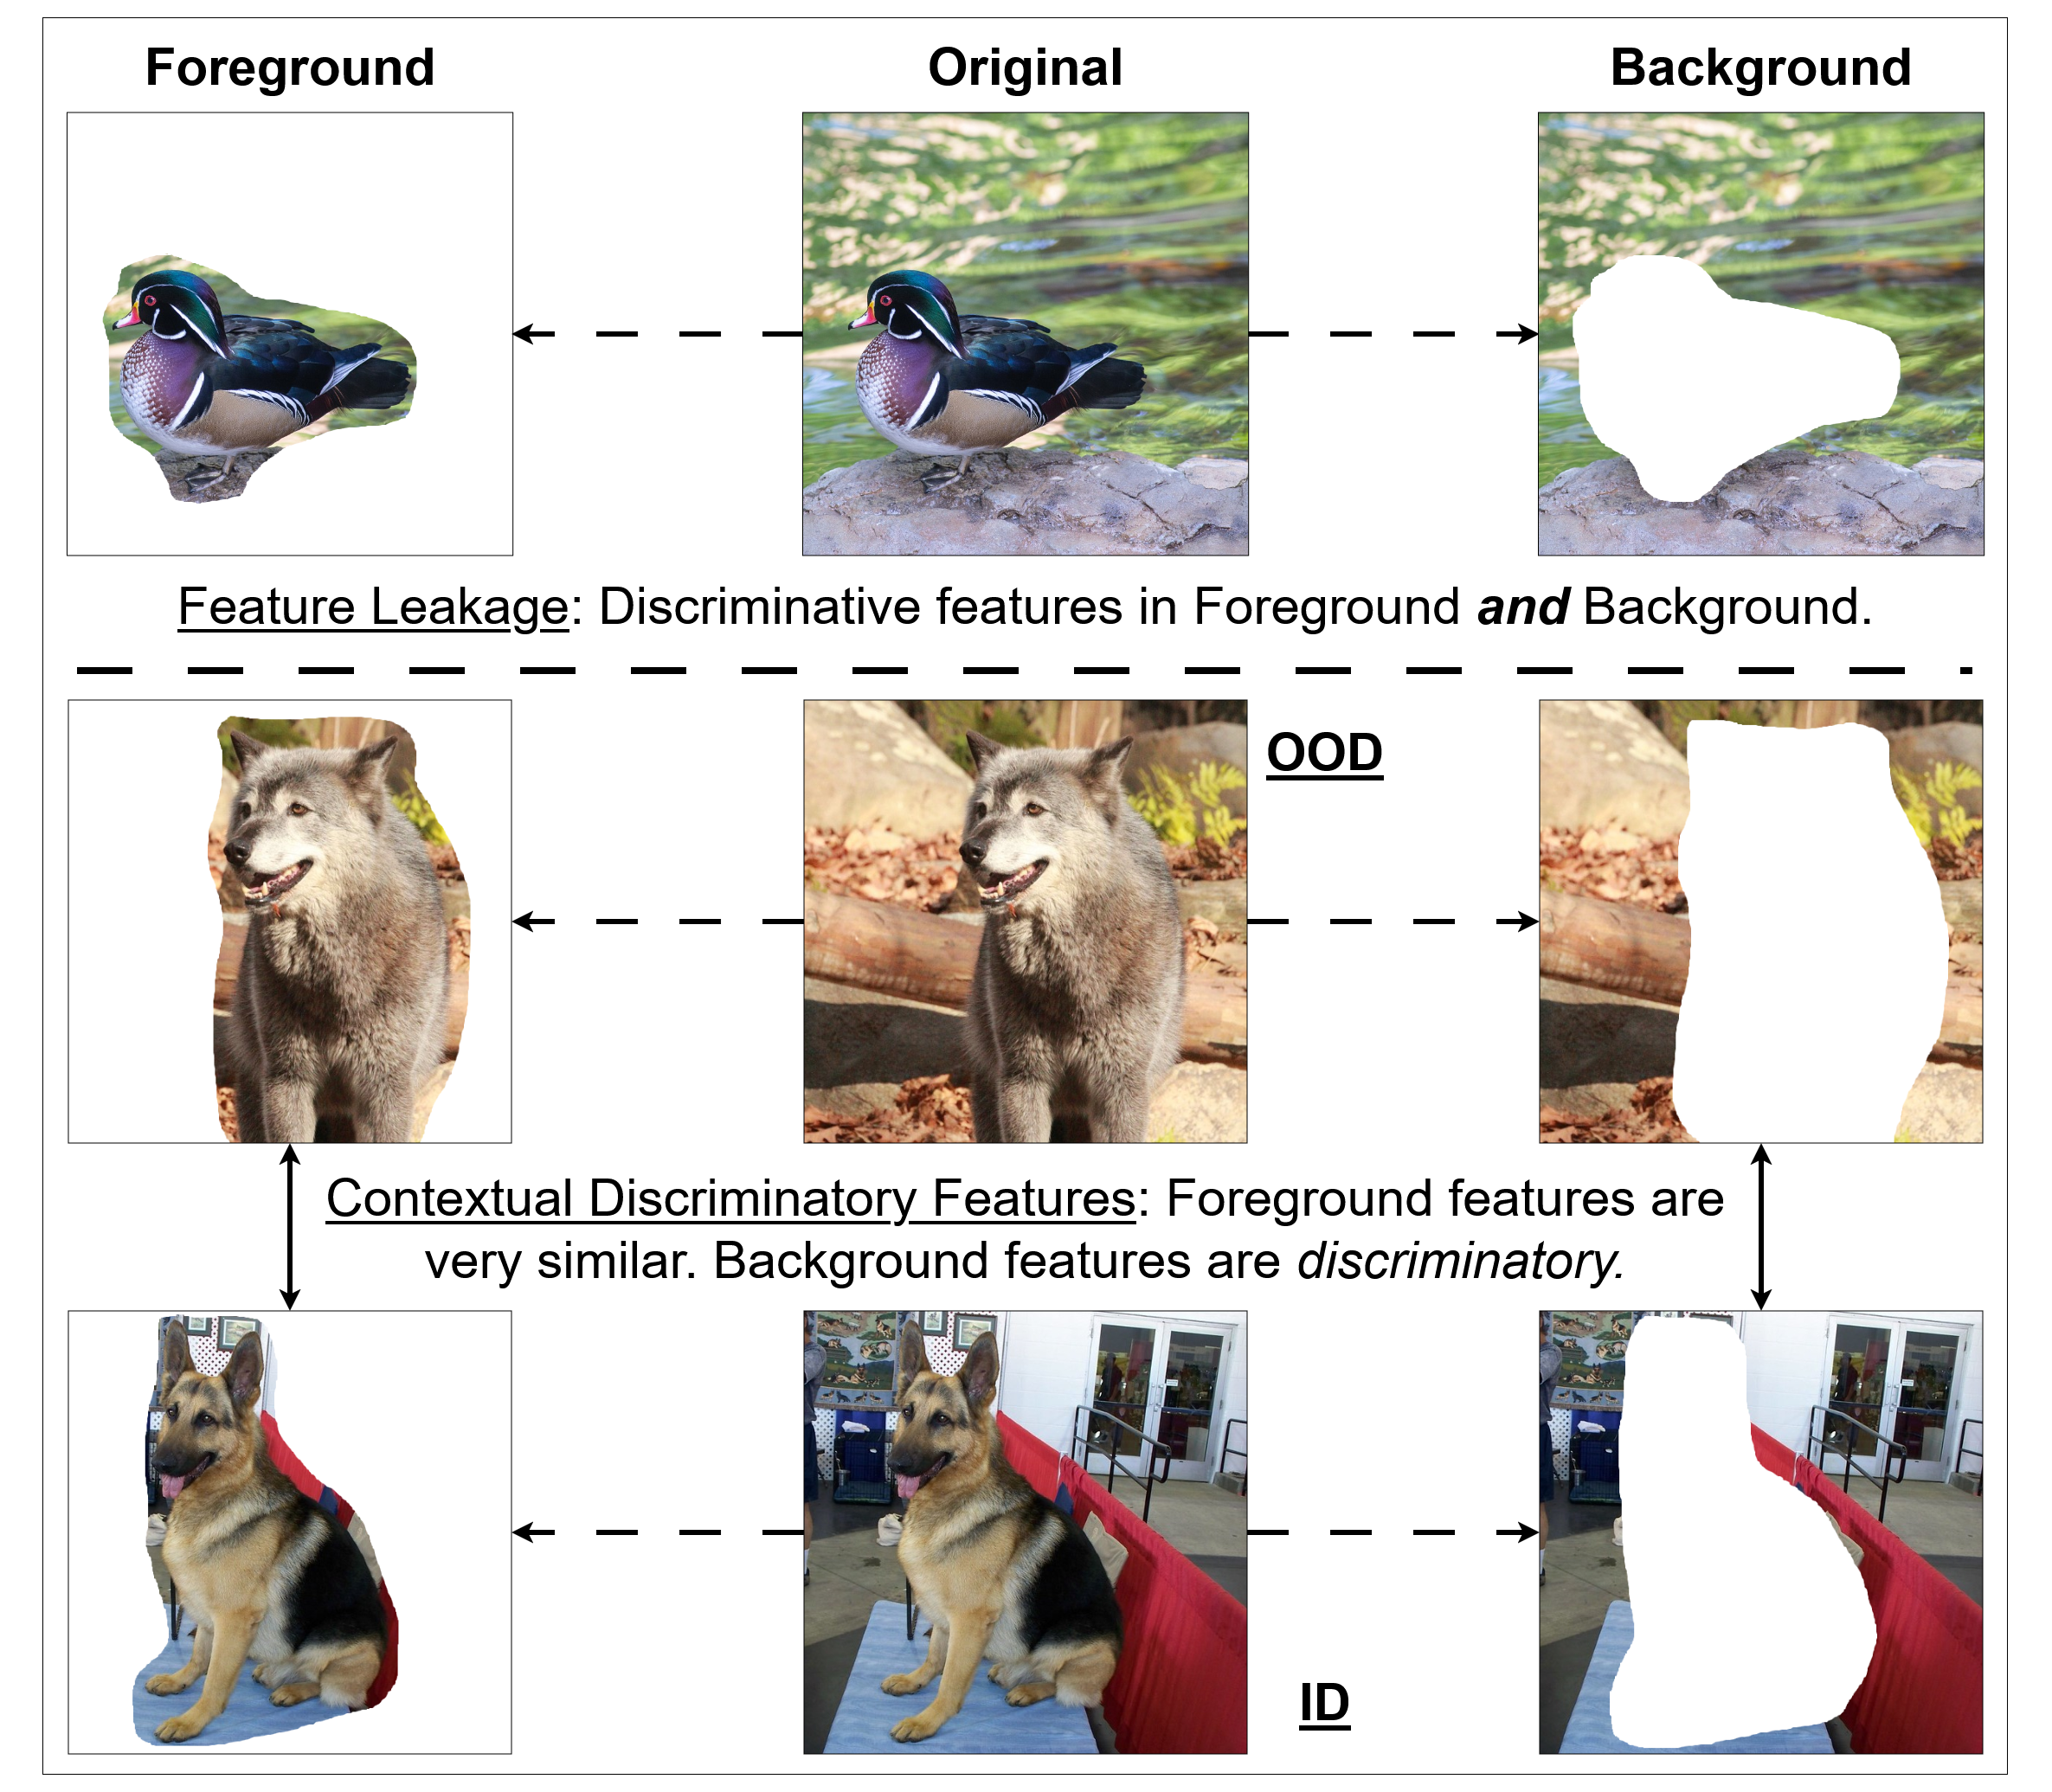
\includegraphics[width=1.\linewidth]{figures/meo_motivation}

  \caption{\sysa fails to account for samples that have ID class-relevant discriminative features in both the foreground \textit{and} the background (top row). Accounting for the discriminative features across foreground-background views in differing capacities is necessary for some near-OOD cases, such as that shown in the bottom section where the background features provide critical contextual information distinguishing the ``wolf'' from the ``dog''.
  }
  \label{fig:propwork-meo-motiv}
\end{figure}

%(shortcomings of MOD: unstable, selection can be easily biased towards/away from certain views) - covered in previous section

%(motivation: if we can train the mv model to extract helpful features from all views then we can include all of them)
%(motivation: also investigate which views are helpful at which points)

%The original motivation for \sysa was to identify and exclusively include whichever view (out of either the foreground or background views) contained more ID class-relevant discriminative features. However, there is no guarantee that such information is located exclusively in one of the views. 
MOD assumes that ID class-relevant discriminative features are exclusively in either the foreground or the background view. It selects one of these views using a view selector before combining it with the original image for OOD detection. However, this assumption is rarely valid. \ref{fig:propwork-meo-motiv} gives two examples where MOD fails to capture the entirety of discriminative features in either of the segmented view. In the first row, distinguishing components of the ``duck'' class are primarily in the foreground view but several important components are also in the background (e.g. the water and the reflections). In the lower section (second and third rows), the ID object discriminative features are all in the foreground views but important contextual features are in the background views. Domestic features in the background help contextualize the ID object of ``dog'' in the foreground against OOD object ``wolf'' which appears similar in the foreground but contains significantly different natural features in the background. Considering \emph{all views} in multi-view OOD detection can be beneficial.

%To investigate the benefits of considering \textit{all} views for OOD detection, the proposed method, \textbf{M}ulti-view \textbf{E}nsemble for \textbf{O}oD detection (\textbf{\sysb}), generates features for all individual views and all combinations of views before evaluating them in ensembles based on ID accuracy and OOD detection performance . Specifically, \sysb extracts view-specific features (called ``single-view features''), fused features of each pair of single-view features (``cross-view features''), and a fused feature of all single-view features (``comprehensive fused feature''). All of these individual and combination fused features are used to generate predictions, and the complete \sysb model is trained end-to-end using an aggregated loss (accounting for all feature predictions). The importance of each view in contributing discriminative features is evaluated through generation of all possible ensembles of learned individual and combination fused features during testing.
The proposed method, %\textbf{M}ulti-view \textbf{E}nsemble for \textbf{O}OD detection (\textbf{\sysb})
Multi-view Ensemble for OOD detection (MEO), investigates this approach by generating features for all possible combinations of views. This set of view combinations (including the views themselves) is systematically evaluated for ID accuracy and OOD detection performance. Specifically, MEO extracts view-specific features (``single-view features''), features fused from pairs of single-view features (``cross-view features''), and a cumulative feature resulting from the fusion of all single-view features (``comprehensive fused feature''). Each of these individual and fused features are learned end-to-end through an aggregate loss and used at test time for ID class prediction and feature-based OOD detection. All possible ensembles of individual and fused features are evaluated for contribution towards learning discriminative features and improving OOD detection.

\subsection{Proposed Method}
\label{sec:propwork-meo-propmeth}

%(proposed architecture with explanation)

%For \sysa, the FgBg multi-view model $f_{MV}$ is implemented using a multi-view convolutional NN (CNN), or MVCNN \cite{su2015multi}, as the backbone. The multi-view feature extractors are each a CNN feature extraction backbone parameterized by $\theta$, $\phi_v = f_{\theta,v}$. Each $f_{\theta,v}$ learn view feature vectors representative of ID class information, taking as input the corresponding view $x_v$ and outputting a $d$-dimensional feature vector $z_v \in \mathbb{R}^d$, $\phi_v: \mathcal{X} \mapsto \mathbb{R}^d$. Here, $V = \{org, fg, bg\}$, and the multi-view feature extractors $\phi_{MV}$ give $Z_{MV} = \{z_{org}, z_{fg}, z_{bg}\}$. The corresponding individual classification weight matrices $W_{MV}$ and biases $b_{MV}$ give $\hat{Y}_{MV} = \{\hat{y}_{org}, \hat{y}_{fg}, \hat{y}_{bg}\}$. In \sysa, the fusion component $\mathcal{U}$ is designed with a view selector, described below, and outputs $z_{\mathcal{U}}$ and $\hat{y}_{\mathcal{U}}$.
MEO resembles MOD in that an MVCNN is used for the FgBg multi-view model $f_{MV}$ backbone. Each feature extractor $\phi_v = f_{\theta,v}$ (parameterized by $\theta$) outputs a $d$-dimensional feature vector from input view $x_v$, $\phi_v: \mathcal{X} \mapsto \mathbb{R}^d$. The multi-view feature extractors $\phi_{MV}$ give $Z_{MV} = \{z_{org}, z_{fg}, z_{bg}\}$ with corresponding classification parameters $W_{MV}$ and $b_{MV}$ subsequently outputting $\hat{Y}_{MV} = \{\hat{y}_{org}, \hat{y}_{fg}, \hat{y}_{bg}\}$. The fusion component $\mathcal{U}$ in MEO differs significantly from MOD, instead constructing the single-view features, cross-view features, and comprehensive fused feature for ensembling.

\begin{figure}
 \centering
 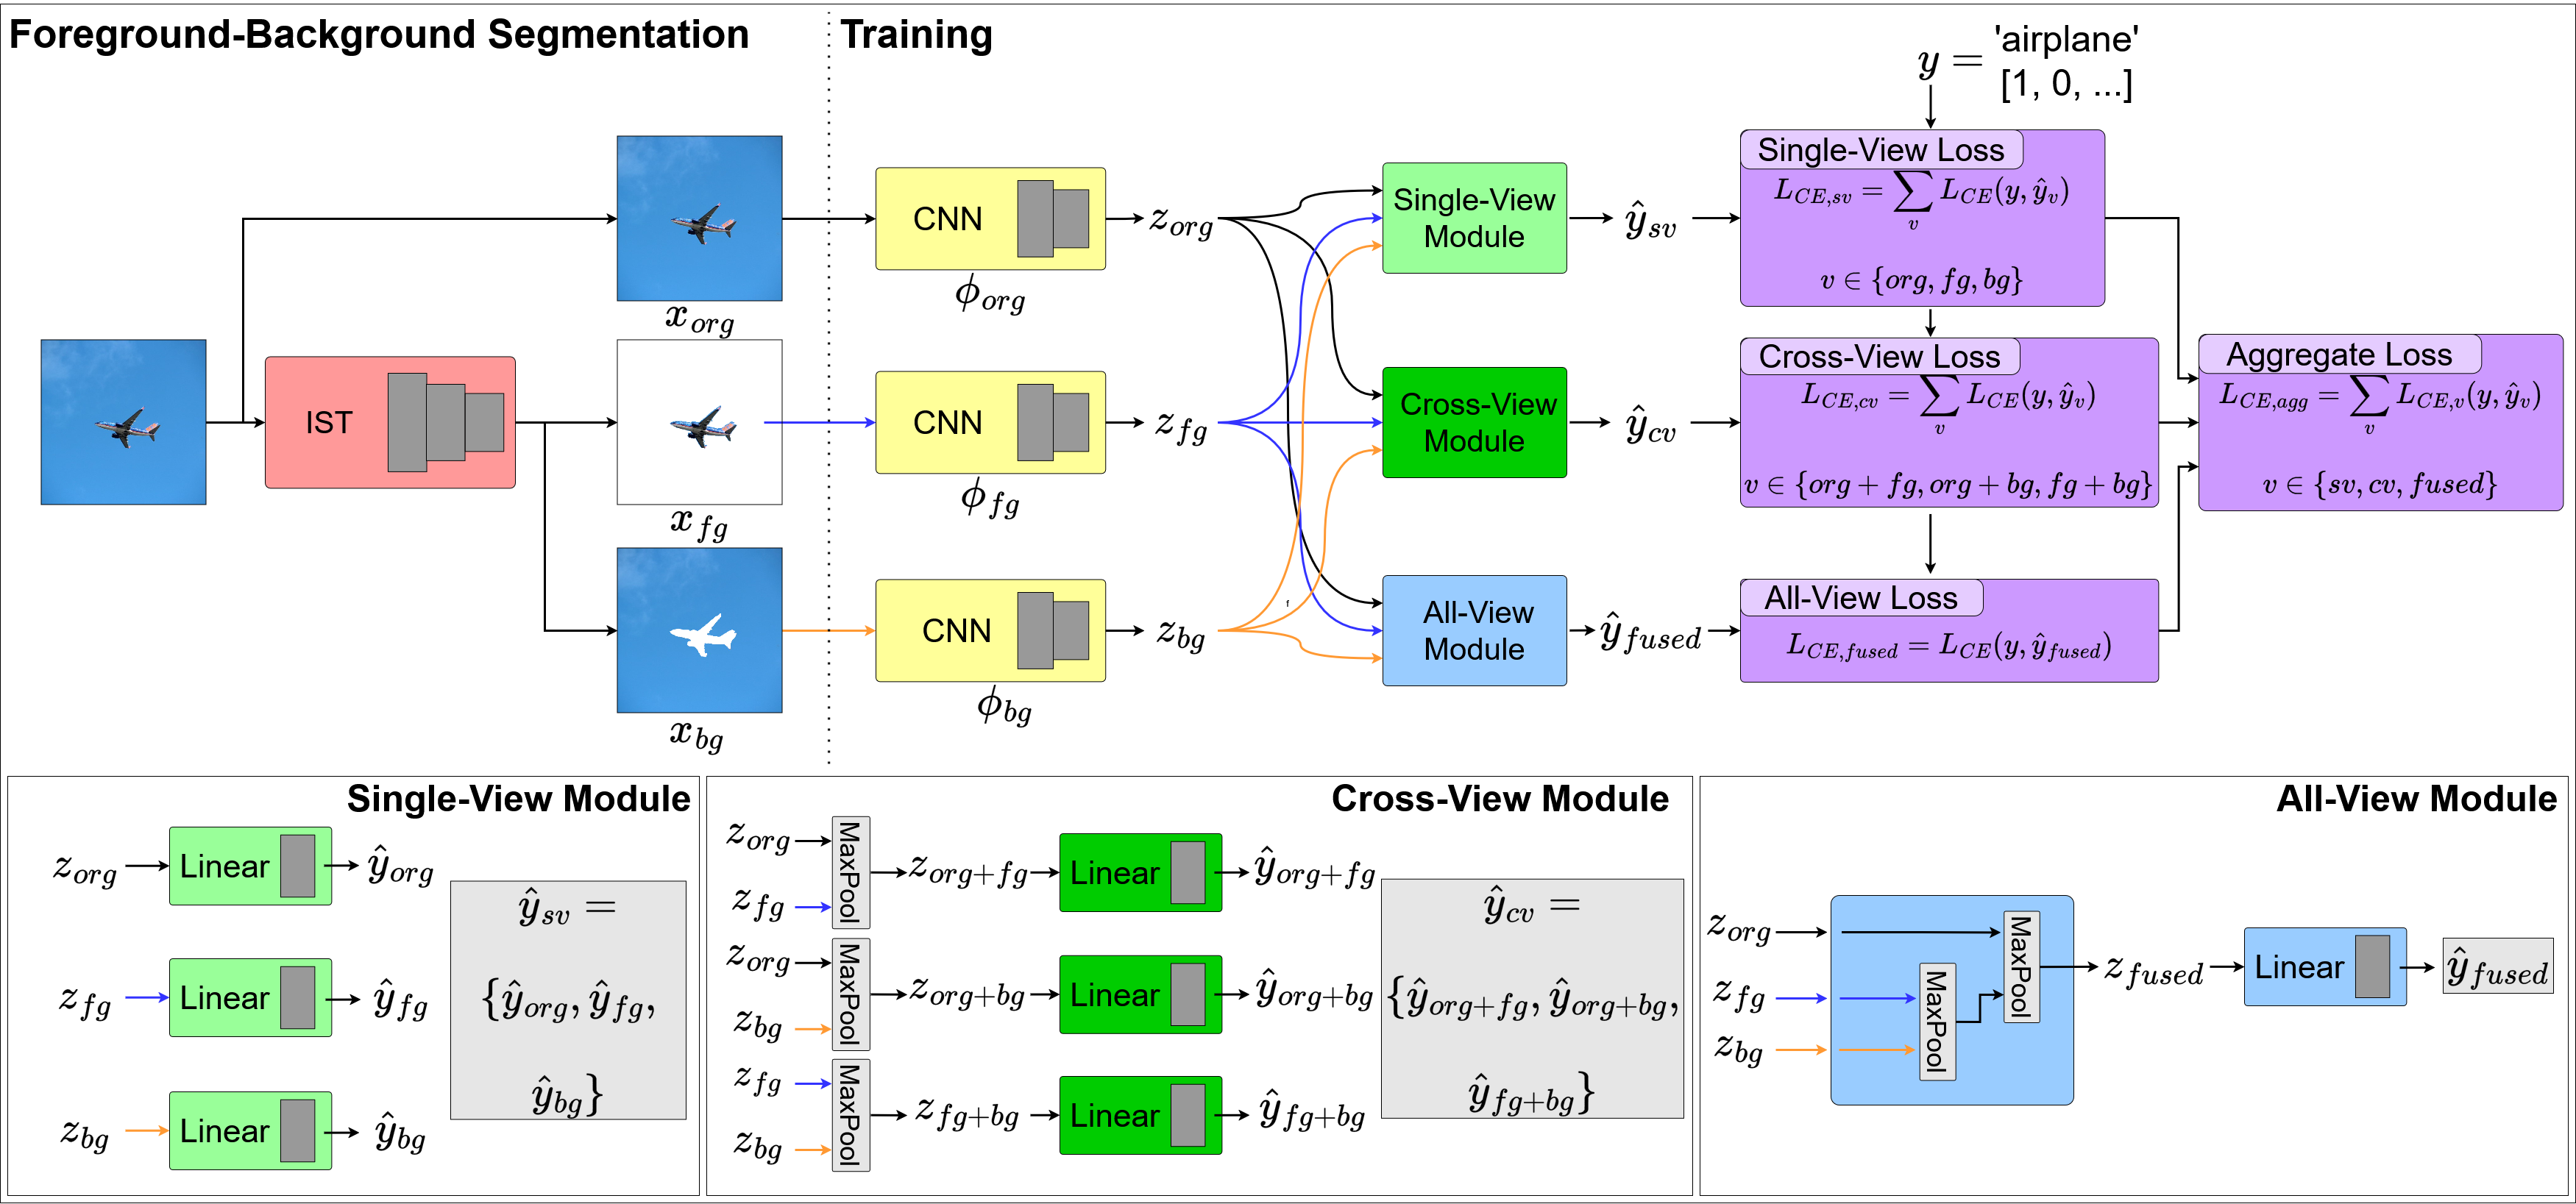
\includegraphics[width=1.\linewidth]{figures/meo_diagram}

  \caption{System diagram of the proposed \sysb. Forward pass is denoted by solid lines and backward pass follows the same lines in the reverse order until the dotted vertical line. %The original or fused image features are denoted by black lines. Foreground image features are denoted by blue lines, background image features are denoted by orange lines. 
  Best viewed in color.
  }
  \label{fig:propwork-meo-diagram}
\end{figure}

%Figure \ref{fig:propwork-meo-diagram} presents the architectural details of \sysb. Similar to \sysa, \sysb uses an MVCNN architecture with three view inputs and corresponding view feature extractors $\phi_{v}$ ($v \in \{org, fg, bg\}$). However, in \sysb the fusion module $\mathcal{G}$ is composed of three separate modules: the Single-View Module, the Cross-View \emph{feature fusion} Module, and the All-View \emph{feature fusion} Module. The Single-View Module does not perform feature fusion. Instead, each view-specific feature vector $z_{org}$, $z_{fg}$, $z_{bg}$ (the single-view features) is passed to a respective linear layer, resulting in three view-specific prediction logits $\hat{y}_{org}$, $\hat{y}_{fg}$, $\hat{y}_{bg}$ (the single-view logits). 
The flow of information for MEO is illustrated in  \ref{fig:propwork-meo-diagram}. The IST segments the original image view (\textit{org}) into a foreground view (\textit{fg}) and a background view (\textit{bg}). The MVCNN backbone generates features $Z_{MV}$ and logits $\hat{Y}_{MV}$. In MEO, the fusion component $\mathcal{U}_{\text{\sysb}}$ is composed of three modules.

\subsubsection{Fusion Component}
The first module in MEO $\mathcal{U}_{\text{\sysb}}$ is the Single-View Module which does not perform fusion, instead simply returning $Z_{MV}$ and $\hat{Y}_{MV}$ (i.e. a no-op).

%In the Cross-View Module, each possible pair of single-view feature vectors, i.e. $\{org+fg, org+bg, fg+bg\}$, is fused using max-pooling. For any two \emph{different} single-view features $z_{v1}$ and $z_{v2}$, the features are combined into a fused feature $z_{v12}$
%\begin{equation}
%\begin{aligned}
%    z_{v12} = \text{MaxPooling}_{p} \{z_{v1}, z_{v2}\}
%\end{aligned}
%\end{equation}
%Fusion in the Cross-View Module results in three cross-view feature vectors $z_{org+fg}$, $z_{org+bg}$, $z_{fg+bg}$. Each of these features is individually passed to respective linear layers, resulting in three cross-view prediction logits $\hat{y}_{org+fg}$, $\hat{y}_{org+bg}$, $\hat{y}_{fg+bg}$.
The second module is the Cross-View Module, in which each possible pair of view-specific feature vectors, $\{org+fg, org+bg, fg+bg\}$, is combined via a max-pooling operation. Given any two \emph{different} view-specific feature vectors $z_{v1}$ and $z_{v2}$, the cross-view feature vector $z_{v12}$ is
\begin{equation}
\begin{aligned}
    z_{v12} = \text{MaxPooling}_{d} \{z_{v1}, z_{v2}\}.
\end{aligned}
\end{equation}
The Cross-View Module in $\mathcal{U}_{\text{\sysb}}$ outputs three cross-view feature vectors $z_{org+fg}$, $z_{org+bg}$, $z_{fg+bg}$, each of which is passed to a respective linear layer with $W_{org+fg}$, $W_{org+bg}$, $W_{fg+bg}$ and $b_{org+fg}$, $b_{org+bg}$, $b_{fg+bg}$. This also results in cross-view predicted logits $\hat{y}_{org+fg}$, $\hat{y}_{org+bg}$, $\hat{y}_{fg+bg}$.

%Finally, the All-View Module uses consecutive max-pooling operations to combine all single-view feature vectors into a single comprehensive fused feature vector
%\begin{equation}
%\begin{aligned}
%    z_{fused} = \text{MaxPooling}_{p}\{z_{org},~\text{MaxPooling}_{p}\{z_{fg},~z_{bg}\}\}
%\end{aligned}
%\end{equation}
%The fused feature $z_{fused}$ is passed to a linear layer, resulting in the comprehensive fused prediction logits $\hat{y}_{fused}$.
The third and final module is the All-View Module. Consecutive max-pooling operations are used to combine all view-specific feature vectors into a single, fused feature vector containing comprehensive information across all views
\begin{equation}
\begin{aligned}
    z_{fused} = \text{MaxPooling}_{d}\{z_{org},~\text{MaxPooling}_{d}\{z_{fg},~z_{bg}\}\}.
\end{aligned}
\end{equation}
$z_{fused}$ is similarly passed to a respective linear layer $W_{fused}$, $b_{fused}$, resulting in $\hat{y}_{fused}$.

%The fusion module $\mathcal{G}$ for \sysb is the composition of all three Single-View, Cross-View, and All-View Modules. Thus the final outputs of the \sysb fusion module $\mathcal{G}$ are the single-view, cross-view, and comprehensive fused feature vectors $Z_{mv} = \{z_{org}, $ $z_{fg}, $ $z_{bg}, $ $z_{org+fg}, $ $z_{org+bg}, $ $z_{fg+bg}, $ $z_{fused}\}$ and the single-view, cross-view, and comprehensive fused prediction logits $\hat{Y}_{mv} = \{\hat{y}_{org}, $ $\hat{y}_{fg}, $ $\hat{y}_{bg}, $ $\hat{y}_{org+fg}, $ $\hat{y}_{org+bg}, $ $\hat{y}_{fg+bg}, $ $\hat{y}_{fused}\}$. For notation convenience, the feature sets are further delineated according to single-view features $z_{sv} = \{z_{org}, z_{fg}, z_{bg}\}$ and cross-view features $z_{cv} = \{z_{org+fg}, z_{org+bg}, z_{fg+bg}\}$.
%At no point in \sysb are the feature extractors frozen while the linear layers are learned (including in the above modules). The entirety of \sysb, i.e. both features and logits, is learned end-to-end.
In summary, the MEO fusion component $\mathcal{U}_{\text{\sysb}}$ utilizes the Single-View, Cross-View, and All-View Modules to output a set of feature vectors $Z_{\mathcal{U}} = \{z_{org}, $ $z_{fg}, $ $z_{bg}, $ $z_{org+fg}, $ $z_{org+bg}, $ $z_{fg+bg}, $ $z_{fused}\}$ and prediction logits $\hat{Y}_{\mathcal{U}} = \{\hat{y}_{org}, $ $\hat{y}_{fg}, $ $\hat{y}_{bg}, $ $\hat{y}_{org+fg}, $ $\hat{y}_{org+bg}, $ $\hat{y}_{fg+bg}, $ $\hat{y}_{fused}\}$. For convenience, feature sets are further delineated according to view-specific features $z_{sv} = \{z_{org}, z_{fg}, z_{bg}\}$ and cross-view features $z_{cv} = \{z_{org+fg}, z_{org+bg}, z_{fg+bg}\}$.

%\textbf{Training:} \sysb is trained end-to-end using a view-aggregate loss $\mathcal{L}_{CE,agg}$ which aggregates the CE losses of all single-view, cross-view, and comprehensive fused predictions.
%
%Given a one-hot true label vector $y$, $\mathcal{L}_{CE,agg}$ is formulated as follows. First, the view-specific CE loss $\mathcal{L}_{CE,sv}$ is defined for each single view $sv \in \{org, fg, bg\}$
%\begin{equation}
%\begin{aligned}
%    \mathcal{L}_{CE,sv}(y, \hat{y}_{sv}) & = -\sum_{c \in \mathcal{Y}} y_{c} \log(\hat{y}_{sv,c}) \\
%\end{aligned}
%\end{equation}
%where $\hat{y}_{sv,c}$ is the logit value of $\hat{y}_{sv}$ for class $c$.
%
%The CE losses for each cross-view $\mathcal{L}_{CE,cv}$, $cv \in \{org+fg, org+bg, fg+bg\}$, is defined similarly
%\begin{equation}
%\begin{aligned}
%    \mathcal{L}_{CE,cv}(y, \hat{y}_{cv}) & = -\sum_{c \in \mathcal{Y}} y_{c} \log(\hat{y}_{cv,c}) \\
%\end{aligned}
%\end{equation}
%
%The comprehensive fused CE loss $\mathcal{L}_{CE,fused}$ is the CE loss of the comprehensive fused prediction logits
%\begin{equation}
%\begin{aligned}
%    \mathcal{L}_{CE,fused}(y, \hat{y}_{fused}) & = -\sum_{c \in \mathcal{Y}} y_{c} \log(\hat{y}_{fused,c}) \\
%\end{aligned}
%\end{equation}
%
%The final aggregate CE loss $\mathcal{L}_{CE,agg}$ is the sum of the above losses
%\begin{equation}
%\begin{aligned}
%    %~org+fg, ~org+bg, ~fg+bg\}}}} \mathcal{L}_{CE,v} (y, \hat{y}_{v})
%    \mathcal{L}_{CE,agg} & = \mathcal{L}_{CE,sv} (y, \hat{y}_{sv}) + \mathcal{L}_{CE,cv} (y, \hat{y}_{cv}) + \mathcal{L}_{CE,fused} (y, \hat{y}_{fused})
%\end{aligned}
%\end{equation}
\subsubsection{Training}
The MEO model is learned end-to-end using a view-aggregate loss $\mathcal{L}_{CE,agg}$. The loss aggregates the classification losses of all single-view, cross-view, and comprehensive fused feature-based predictions. At no point is any component or set of parameters in MEO frozen while other parameters are trained.

A one-hot true label vector $y$ is used to train MEO via $\mathcal{L}_{CE,agg}$ through each set of view features. Specifically, a view-specific CE loss $\mathcal{L}_{CE,sv}$ is defined for each $sv \in \{org, fg, bg\}$
\begin{equation}
\begin{aligned}
    \mathcal{L}_{CE,sv}(y, \hat{y}_{sv}) & = -\sum_{c \in \mathcal{Y}} y_{c} \log(\hat{y}_{sv,c}). \\
\end{aligned}
\end{equation}
$\hat{y}_{sv,c}$ is the logit value of $\hat{y}_{sv}$ for class $c$.

Cross-views $cv \in \{org+fg, org+bg, fg+bg\}$ are accounted for through CE loss $\mathcal{L}_{CE,cv}$
\begin{equation}
\begin{aligned}
    \mathcal{L}_{CE,cv}(y, \hat{y}_{cv}) & = -\sum_{c \in \mathcal{Y}} y_{c} \log(\hat{y}_{cv,c}). \\
\end{aligned}
\end{equation}

The comprehensive fused information is accounted for through CE loss $\mathcal{L}_{CE,fused}$
\begin{equation}
\begin{aligned}
    \mathcal{L}_{CE,fused}(y, \hat{y}_{fused}) & = -\sum_{c \in \mathcal{Y}} y_{c} \log(\hat{y}_{fused,c}). \\
\end{aligned}
\end{equation}

These CE losses are combined in the final aggregate CE loss $\mathcal{L}_{CE,agg}$
\begin{equation}
\begin{aligned}
    %~org+fg, ~org+bg, ~fg+bg\}}}} \mathcal{L}_{CE,v} (y, \hat{y}_{v})
    \mathcal{L}_{CE,agg} & = \mathcal{L}_{CE,sv} (y, \hat{y}_{sv}) + \mathcal{L}_{CE,cv} (y, \hat{y}_{cv}) + \mathcal{L}_{CE,fused} (y, \hat{y}_{fused}).
\end{aligned}
\end{equation}

%\textbf{OOD Detection:} \sysb uses the MD OOD score for the same reasons as \sysa, i.e. the use of multiple views constructs a rich feature space specially suited for distance-based OOD detection methods. Note that while only MD is considered in this proposed work as a representative technique, \sysb is compatible with other distance-based OOD detection methods as well.
%
%The definition of MD for \sysb is identical to that of \sysa (see Section \ref{sec:propwork-mod-propmeth}). However, instead of only generating empirical class means and a covariance matrix for the comprehensive fused feature $z_{fused}$, \sysb calculates empirical class means $\hat{\mu}_{c,v}$ and covariance matrices $\hat{\Sigma}_{v}$ for each view feature $v \in \{org, fg, bg, org+fg, org+bg, fg+bg, fused\}$. Given a test instance $x'$, \sysb extracts the feature vector $z'_{v}$ and computes the distance between it and the nearest class-conditional Gaussian distribution for the view $v$. The negative of this distance is the final OOD score for view $v$
%\begin{equation}
%\begin{aligned}
%    M_{MD,v}(x') = \max_{c} (-(z_{v}' - \hat{\mu}_{c,v})^\top \hat{\Sigma}_{v}^{-1} (z_{v}' - \hat{\mu}_{c,v})) \\
%\end{aligned}
%\end{equation}
\subsubsection{OOD Detection}
Following from MOD (see Section \ref{sec:propwork-mod-propmeth}), MEO leverages distance-based OOD detection methods to exploit the rich feature space learned from the use of foreground-background segmented views. MEO is compatible with all distance-based (and otherwise post-hoc) OOD detection methods that operate on features and/or logits. However, this work only presents results for MD.

The implementation of MD for MEO is very similar to that in MOD. However, given that MEO uses a combination of view-specific features, cross-view features, and a comprehensive fused feature, multiple empirical class means and covariance matrices must be defined. MEO calculates empirical class means $\hat{\mu}_{C,v}$ and covariance matrices $\hat{\Sigma}_{v}$ for each view feature $v \in \{org, fg, bg, org+fg, org+bg, fg+bg, fused\}$. A test sample $x'$ is processed by MEO into feature vector $z'_{v}$. Distances are computed between $z'_{v}$ and the nearest class-conditional Gaussian distribution for view $v$. The negative distance is the OOD score for view $v$
\begin{equation}
\begin{aligned}
    S_{MD,v}(x') = \max_{c} (-(z_{v}' - \hat{\mu}_{c,v})^\top \hat{\Sigma}_{v}^{-1} (z_{v}' - \hat{\mu}_{c,v})). \\
\end{aligned}
\end{equation}

%(ensembles definitions)

\subsubsection{Single-, Cross-, and Comprehensive Fused View Ensembling}

%During testing, all possible combinations of view feature vectors, i.e. $z_{sv}$, $z_{cv}$, and $z_{fused}$, and prediction logits, i.e. $\hat{y}_{sv}$, $\hat{y}_{cv}$, and $\hat{y}_{fused}$, are considered. An ensemble $E$ is defined as the combination of view members, i.e. $E \subseteq \{org, fg, bg, org+fg, org+bg, fg+bg, fused\}$. Any given ensemble $E$ has access to all prediction logits $\hat{y}_{e}$ and MD OOD scores $M_{MD,e}$ for its members $e \in E$.
All possible combinations of MEO feature vectors $z_{sv}$, $z_{cv}$, $z_{fused}$ and prediction logits $\hat{y}_{sv}$, $\hat{y}_{cv}$, and $\hat{y}_{fused}$ are considered during test-time evaluation. An ensemble $\mathcal{E}$ is defined as the set of members composed of views, $\mathcal{E} \subseteq \{org, fg, bg, org+fg, org+bg, fg+bg, fused\}$. An ensemble $\mathcal{E}$ outputs prediction logits $\hat{y}_{e}$ and MD OOD scores $S_{MD,e}$ for each member $e \in \mathcal{E}$.

%For ID classification, \sysb combines all ensemble $E$'s members prediction logits $\hat{y}_{e}$ by applying a softmax operation on each ensemble member $e$'s logits before taking the element-wise product of all resultant prediction distributions
%\begin{equation}
%\begin{aligned}
%    \hat{y}_{ens} & = \prod_{e ~\in~ E} \sigma(\hat{y}_{e}) \\
%\end{aligned}
%\end{equation}
%where $\hat{y}_{ens}$ is a vector representing the final ensemble prediction result and $\sigma(\hat{y}_{e})$ is the softmax operation on each ensemble member prediction logits $\hat{y}_{e}$.
\subsubsection{Ensemble ID Classification}
MEO combines all ensemble $\mathcal{E}$'s member prediction through element-wise product of all softmax logits $\text{softmax}(\hat{y}_{e})$
\begin{equation}
\begin{aligned}
    \hat{y}_{\mathcal{E}} & = \prod_{e ~\in~ \mathcal{E}} \text{softmax}(\hat{y}_{e}). \\
\end{aligned}
\end{equation}
Note that $\hat{y}_{\mathcal{E}}$ is the final prediction vector for ensemble $\mathcal{E}$ resulting from the combination of all member prediction distributions. %$\text(softmax)$ is the softmax operation on a vector.

%For OOD detection, \sysb takes the mean across all ensemble $E$'s members MD OOD scores $M_{MD,e}(x')$ for a given test instance $x'$
%\begin{equation}
%\begin{aligned}
%    M_{MD,ens}(x') & = \frac{1}{\lvert E \rvert} \sum_{e ~\in~ E} M_{MD,e}(x') \\
%\end{aligned}
%\end{equation}
%where $M_{MD,ens}$ is the final ensemble MD OOD score.
%
%It is important to note that the cross-view features and predictions are \emph{not} simply degenerate ensembles of their components, e.g. $z_{fg+bg}$ is not semantically identical to the ensemble of $z_{fg}$ and $z_{bg}$. Each view feature is trained using a separate linear layer prediction head and is a unique fusion of its single-view feature components. Therefore, the cross-view feature vectors encode unique data relevant to both the view itself and the data sample.
\subsubsection{Ensemble OOD Detection}
The ensemble $\mathcal{E}$ OOD score is the mean across all member MD OOD scores $S_{MD,e}(x')$ for test sample $x'$
\begin{equation}
\begin{aligned}
    S_{MD,\mathcal{E}}(x') & = \frac{1}{\lvert \mathcal{E} \rvert} \sum_{e ~\in~ \mathcal{E}} S_{MD,e}(x'). \\
\end{aligned}
\end{equation}
Note that $S_{MD,\mathcal{E}}$ is the final OOD score for ensemble $\mathcal{E}$.

Cross-view features and predictions semantically represent more than their separate components. For example, $z_{fg+bg}$ is not identical to the ensemble $\mathcal{E} = \{z_{fg}, z_{bg}\}$. Each view (single-view, cross-view, or comprehensive fused) is trained using a distinct prediction linear layer on top of being a unique fusion of view-specific components. Thus, cross-view feature vectors contain unique discriminative feature information relevant to the ID class.

\subsection{Experiments}
\label{sec:propwork-meo-exp}

%(CIFAR-100 results: near- and far-ood)

%The evaluation of \sysb follows a nearly identical experimental setup as that of \sysa. Deviations are described accordingly in each relevant section.
The experimental settings from MOD are used for MEO, with minor deviations (noted where appropriate). %Full results on all possible ensembles $\mathcal{E}$ are presented in the Appendix (see Appendix Section \ref{}{\color{red}TODO}).

%\textbf{Datasets:} CIFAR-100 \cite{krizhevsky2009learning} remains as the training and ID testing dataset. The SVHN \cite{yuval2011reading} dataset is added as a far-OOD dataset.
\subsubsection{Datasets}
CIFAR-10 and CIFAR-100 \cite{krizhevsky2009learning} are used as training and ID testing datasets. SVHN \cite{yuval2011reading} is added as a far-OOD dataset. ImageNet-30 \cite{russakovsky2015imagenet} is also added as a training and ID testing dataset. OOD datasets for ImageNet-30 follow previous experimental work \cite{li2023rethinking,yang2022openood} and include CIFAR-10, CIFAR-100, SVHN, LSUN, Textures, Places365, iNaturalist, and Tiny ImageNet. ImageNet-30 is not used as an OOD dataset for the CIFAR ID experimental settings because it has significantly higher resolution and image size, making the data domains incomparable.

%\textbf{Baselines:} Additional state-of-the-art baselines were included for the \sysb experiments: Optimal Parameter and Neuron Pruning (OPNP) \cite{chen2024optimal}, Orthogonal Gradient Projection (GradOrth) \cite{behpour2024gradorth}, and Adaptive Temperatue Scaling (ATS) \cite{krumpl2024ats}. Their results are directly copied from the respective papers as none of them provide code for reproduction and their experimental setups are the same.
\subsubsection{Baselines}
For MEO experiments, additional state-of-the-art baseline methods were considered. Specifically, Optimal Parameter and Neuron Pruning (OPNP) \cite{chen2024optimal}, Orthogonal Gradient Projection (GradOrth) \cite{behpour2024gradorth}, and Adaptive Temperatue Scaling (ATS) \cite{krumpl2024ats} were included based on their recent results. Results for these additional baselines are copied from respective papers, as their experimental setups are the same and code was either not available or failed to converge.

\subsection{Results}
\label{sec:propwork-meo-results}

%((if space) VERY BASIC analysis/conclusions on results)

\begin{table*}
\small
\centering
\caption{CIFAR-10 ID classification (\textbf{Accuracy}) and OOD detection performance (\textbf{AUC}) comparison between top-3 \sysb ensembles and recent state-of-the-art baselines on \textit{near-OOD} datasets. %All numeric values are percentages. Best results are emphasized with \textbf{boldface}. 
The following key is used to shorten ensemble members: ``\textbf{f}'' - comprehensive fused feature/logits, ``\textbf{O}'' - original single-view, ``\textbf{F}'' - foreground single-view, ``\textbf{B}'' - background single-view, ``\textbf{OF}'' - $org+fg$ cross-view, ``\textbf{OB}'' - $org+bg$ cross-view, and ``\textbf{FB}'' - $fg+bg$ cross-view. For example, a ``f+OF+OB'' ensemble would have members $\{fused$, $org+fg$, $org+bg\}$. This notation is used consistently throughout the rest of the dissertation with respect to \sysb.
}
\vspace{0.1cm}
\scalebox{1.0}{
\begin{tabular}{|l|c|ccc|}
\hline
\multicolumn{1}{|c|}{\multirow{2}{*}{}} & ID & \multicolumn{3}{c|}{OOD}    \\ \cline{2-5} 
\multicolumn{1}{|l|}{} & CIFAR-10   & CIFAR-100  & Tiny ImageNet  & \multicolumn{1}{|c|}{Average}   \\ \hline
MSP       & 94.73$_{\pm 0.11}$ &  87.05$_{\pm 0.51}$   &  \multicolumn{1}{c|}{87.98$_{\pm 0.34}$}   & 87.51  \\  
KNN       & 94.73$_{\pm 0.11}$ & 89.55$_{\pm 0.22}$   &  \multicolumn{1}{c|}{90.15$_{\pm 0.14}$}   &  89.85  \\  
MD        & 94.73$_{\pm 0.11}$ & 83.33$_{\pm 0.72}$   &  \multicolumn{1}{c|}{83.68$_{\pm 0.68}$}   &   83.51 \\  
ViM       & 94.73$_{\pm 0.11}$ &  86.39$_{\pm 1.72}$   &  \multicolumn{1}{c|}{87.26$_{\pm 1.56}$}   &  86.82 \\ 
React     & 94.73$_{\pm 0.11}$ &  84.82$_{\pm 1.39}$   &  \multicolumn{1}{c|}{86.76$_{\pm 0.98}$}   &   85.79  \\  
FeatNorm  & 94.73$_{\pm 0.11}$ & 88.89$_{\pm 0.66}$  & \multicolumn{1}{c|}{90.16$_{\pm 0.81}$}   &  89.53   \\  
GEN       & 94.73$_{\pm 0.11}$ & 87.19$_{\pm 0.58}$   &  \multicolumn{1}{c|}{88.56$_{\pm 0.40}$}   &   87.87 \\  
LogitNorm & 94.56$_{\pm 0.22}$ & 90.80$_{\pm 0.82}$ &  \multicolumn{1}{c|}{91.80$_{\pm 0.65}$}   &   91.30 \\
CSI       & / &  92.2  &  97.6  & \multicolumn{1}{|c|}{94.90}  \\  
CMG-e     & / & 89.3 &  95.2  & \multicolumn{1}{|c|}{92.25} \\ \hline
MOD-MD  & 95.37$_{\pm 0.29}$ & 95.54$_{\pm 5.39}$ & \multicolumn{1}{c|}{96.34$_{\pm 2.60}$}  & 95.94  \\ \cdashline{1-5}
MEO-MD & & & & \multicolumn{1}{|c|}{} \\ %\cline{1-1} %\hline
f+O+F+OB    & 95.08$_{\pm 0.40}$ & \textbf{99.28$_{\pm 0.64}$} & 98.60$_{\pm 1.56}$ &  \multicolumn{1}{|c|}{\textbf{98.94}} \\ 
f+O+F+OF+OB & 94.95$_{\pm 0.34}$ & 99.00$_{\pm 0.52}$ & \textbf{98.76$_{\pm 1.45}$} &  \multicolumn{1}{|c|}{98.88}  \\ 
f+F+B+OB+FB & \textbf{95.24$_{\pm 0.39}$} & 99.09$_{\pm 0.64}$ & 98.50$_{\pm 1.59}$ &  \multicolumn{1}{|c|}{98.80}  \\ \hline
\end{tabular}
}
\label{tab:propwork-meo-results-cifar10-near}
\end{table*}

\begin{table*}
\small
\centering
\caption{CIFAR-10 OOD detection performance (\textbf{AUC}) comparison between top-3 \sysb ensembles and recent state-of-the-art baselines on \textit{far-OOD} datasets. %All numeric values are percentages. Best results are emphasized with \textbf{boldface}.
}
\vspace{0.1cm}
\scalebox{0.875}{
\begin{tabular}{|l|cccccc|}
\hline
\multicolumn{1}{|l|}{\multirow{2}{*}{}} &   \multicolumn{6}{c|}{OOD}   \\ \cline{2-7}
\multicolumn{1}{|l|}{}   &  SVHN &   LSUN & Textures  & Places365 & iNaturalist & \multicolumn{1}{|c|}{Average}  \\ \hline
MSP    & 93.39$_{\pm 2.30}$ &  90.45$_{\pm 0.42}$  & 92.01$_{\pm 0.58}$  & 89.88$_{\pm 0.55}$  & \multicolumn{1}{c|}{90.20$_{\pm 0.73}$}   & 91.18  \\  
KNN    & 95.45$_{\pm 1.38}$   &  92.29$_{\pm 0.15}$   & 94.24$_{\pm 0.40}$   & 91.46$_{\pm 0.25}$   & \multicolumn{1}{c|}{91.73$_{\pm 0.62}$}  & 93.03  \\  
MD     & 99.10$_{\pm 0.46}$  & 85.48$_{\pm 0.74}$ & 96.81$_{\pm 0.32}$   & 82.77$_{\pm 0.80}$ & \multicolumn{1}{c|}{87.31$_{\pm 1.57}$}  &  90.30   \\  
ViM    & 97.57$_{\pm 2.24}$   & 89.26$_{\pm 2.05}$ & 96.05$_{\pm 1.04}$ & 88.05$_{\pm 1.96}$ & \multicolumn{1}{c|}{89.96$_{\pm 1.27}$}   & 92.18   \\  
React  & 93.80$_{\pm 1.75}$ &  91.47$_{\pm 0.55}$   & 90.67$_{\pm 0.89}$   & 89.57$_{\pm 1.11}$   & \multicolumn{1}{c|}{87.94$_{\pm 2.30}$}   &  90.69  \\  
FeatNorm   & 99.07$_{\pm 0.40}$ & 91.93$_{\pm 1.15}$  & 94.61$_{\pm 0.23}$   & 95.37$_{\pm 0.41}$   & \multicolumn{1}{c|}{94.14$_{\pm 1.31}$}  &  95.03  \\  
GEN         & 94.15$_{\pm 2.17}$  &  91.35 $_{\pm 0.53}$  & 92.53$_{\pm 0.79}$   & 90.82$_{\pm 0.65}$  & \multicolumn{1}{c|}{90.97$_{\pm 0.90}$}   &  91.96   \\  
LogitNorm & 97.61$_{\pm 0.92}$  &  95.06$_{\pm 0.59}$  & 94.53$_{\pm 1.07}$  & 95.66$_{\pm 0.42}$   & \multicolumn{1}{c|}{93.18$_{\pm 1.05}$}   &   95.21  \\
OPNP       &  \textbf{99.90} &  /  & 98.20  & 97.64  & \multicolumn{1}{c|}{/}   &   /  \\ 
GradOrth  &  98.72 & / & 94.77  & 91.64   & \multicolumn{1}{c|}{/}   &   / \\ \hline
MOD-MD  & / & 96.02$_{\pm 2.97}$ & 98.42$_{\pm 1.12}$ & 95.90$_{\pm 3.04}$ & 98.63$_{\pm 0.57}$ & \multicolumn{1}{|c|}{97.24} \\ \cdashline{1-7}
MEO-MD & & & & & & \multicolumn{1}{|c|}{}  \\
f+O+F+OB    & 97.67$_{\pm 2.61}$ & 99.29$_{\pm 0.53}$ & 99.87$_{\pm 0.10}$ & 99.62$_{\pm 0.30}$ & \textbf{99.97$_{\pm 0.02}$} &  \multicolumn{1}{|c|}{99.29}    \\ 
f+O+F+OF+OB  & 98.34$_{\pm 1.22}$ & \textbf{99.40$_{\pm 0.43}$} & \textbf{99.90$_{\pm 0.09}$} & \textbf{99.66$_{\pm 0.22}$} & \textbf{99.97$_{\pm 0.02}$} &  \multicolumn{1}{|c|}{\textbf{99.45}}      \\ 
f+F+B+OB+FB & 97.74$_{\pm 2.17}$  &  99.19$_{\pm 0.56}$ & 99.86$_{\pm 0.10}$ & 99.49$_{\pm 0.33}$ & 99.96$_{\pm 0.03}$ &  \multicolumn{1}{|c|}{99.25}       \\  \hline
\end{tabular}
}
\label{tab:propwork-meo-results-cifar10-far}
\end{table*}

%\begin{figure}[tb]
%  \center
%\includegraphics[width=0.82\linewidth]{figures/mvens_view_distances}
%  \caption{
%  MDs for ID test (CIFAR-100) and OOD (Tiny ImageNet) data for each single-view. The distances for $B$ are 1) significantly larger than that of either $O$ or $F$ for OOD data, and 2) significantly larger for the OOD data than that of the ID data. Note that the data samples are sorted according to their MD distances from large to small. 
%  }
%  \vspace{-4mm}
%  \label{fig:propwork-meo-results-fgbg_contrib}
%\end{figure}

%Results of the \sysb experiments are shown in Table \ref{tab:propwork-meo-results-cifar100-far} (far-OOD datasets) and Table \ref{tab:propwork-meo-results-cifar100-near} (near-OOD datasets). To conserve space, only the top-3 \sysb ensembles are presented. %The full tables containing results for all possible \sysb ensembles is provided in \textcolor{blue}{TODO - ref to additional results... should we? or leave that for future work?}. 
%\sysb substantially outperforms state-of-the-art baselines in OOD detection. For far-OOD datasets (Table \ref{tab:propwork-meo-results-cifar100-far}), all \sysb ensembles improve the average AUROC (maximum improvement of 16.40\%) as well as the AUROC of each individual OOD dataset except SVHN. For near-OOD datasets (Table \ref{tab:propwork-meo-results-cifar100-near}), \sysb ensembles again outperform baselines, with the $f+O+F+OF+OB$ ensemble improving average AUROC by 9.82\%, CIFAR-10 AUROC by 2.93\%, and Tiny ImageNet AUROC by 9.51\%. \sysb also benefits ID classification, with all top-3 \sysb ensembles improving accuracy (maximum improvement of 0.97\%). An interesting observation from the top \sysb ensembles is that each ensemble includes at least one single-view feature, at least one cross-view feature, and the comprehensive fused feature. This suggests that all of the individual and combination fused features contain discriminative features important to representing ID class-relevant information and distinguishing OOD instances.
\ref{tab:propwork-meo-results-cifar10-near} (near-OOD datasets) and \ref{tab:propwork-meo-results-cifar10-far} (far-OOD datasets) show results for the MEO experiments on CIFAR-10. Only the top-3 MEO ensembles are presented in this section. Previous state-of-the-art baselines are unable to outperform MEO in OOD detection. 
In the near-OOD domain (\ref{tab:propwork-meo-results-cifar10-near}), the top MEO ensembles outperform all baselines. In particular, the $f+O+F+OB$ ensemble improves the average AUC by 4.04\%, AUC of CIFAR-100 by 7.08\%, and AUC of Tiny ImageNet by 1.00\%. Across the top-3 ensembles, performance is consistent. Variance of AUC is only 0.02\% for CIFAR-100, 0.02\% for Tiny ImageNet, and 0.005\% on average. MEO ensembles also outperform MOD, validating the idea of utilizing feature information in \emph{all} views for OOD detection instead of selectively eliminating views. The $f+O+F+OB$ MEO ensemble improves the average CIFAR-10 near-OOD AUC by 3.00\%, from 95.94\% to 98.94\%, a significant margin.
In the far-OOD domain (\ref{tab:propwork-meo-results-cifar10-far}), MEO ensembles again improve AUC both on average (4.24\%) and across individual datasets (except SVHN), where the $f+O+F+OF+OB$ ensemble underperforms by only 1.56\% (and still achieves a high AUC of 98.34\%). On the challenging iNaturalist far-OOD dataset, MEO ensembles perform extremely well, each improving AUC by 5.81-5.82\% over the nearest state-of-the-art baseline. Variance across the top-3 MEO ensembles is again low, only 0.01\% for average OOD detection performance. Similar to the near-OOD CIFAR-10 datasets, MEO ensembles improve on MOD, improving average OOD detection by 2.21\% and demonstrating a particularly large increase in Places365 of 3.76\%.
ID classification is also unaffected by the multi-view paradigm. All 3 top MEO ensembles improve ID classification accuracy (maximum improvement of 0.68\%), demonstrating that MEO is able to learn ID class-relevant discriminative features effective for OOD detection while maintaining ID classification functionality.

\begin{table*}
\small
\centering
\caption{CIFAR-100 ID classification (\textbf{Accuracy}) and OOD detection performance (\textbf{AUC}) comparison between top-3 \sysb ensembles and recent state-of-the-art baselines on \textit{near-OOD} datasets. %All numeric values are percentages. Best results are emphasized with \textbf{boldface}.
}
\vspace{0.1cm}
\scalebox{1.0}{
\begin{tabular}{|l|c|ccc|}
\hline
\multicolumn{1}{|c|}{\multirow{2}{*}{}} & ID &  \multicolumn{3}{c|}{OOD}    \\ \cline{2-5} 
\multicolumn{1}{|l|}{} & CIFAR-100  & CIFAR-10 & Tiny ImageNet & \multicolumn{1}{|c|}{Average}   \\ \hline
MSP       & 77.66$_{\pm 0.43}$  &  78.99$_{\pm 0.20}$  & \multicolumn{1}{c|}{80.74$_{\pm 0.26}$}  &  79.87 \\  
KNN       &  77.66$_{\pm 0.43}$ &  77.42$_{\pm 0.36}$ & \multicolumn{1}{c|}{81.67$_{\pm 0.16}$}   &   79.54 \\  
MD        &   77.66$_{\pm 0.43}$&  77.71$_{\pm 0.78}$  & \multicolumn{1}{c|}{75.26$_{\pm 1.21}$}   &   76.49 \\  
ViM       &  77.66$_{\pm 0.43}$ &  71.71$_{\pm 0.94}$ & \multicolumn{1}{c|}{76.06$_{\pm 0.58}$}   &     73.88 \\ 
ReAct     &  77.66$_{\pm 0.43}$ &  78.33$_{\pm 1.36}$  & \multicolumn{1}{c|}{79.00$_{\pm 0.44}$}   &  78.66 \\  
FeatNorm  &  77.66$_{\pm 0.43}$ & 59.81$_{\pm 1.53}$ & \multicolumn{1}{c|}{52.05$_{\pm 2.58}$}   &  55.93   \\  
GEN       &  77.66$_{\pm 0.43}$ & 80.71$_{\pm 0.47}$ & \multicolumn{1}{c|}{80.99$_{\pm 0.37}$}   &   80.85\\  
LogitNorm & 75.92$_{\pm 0.55}$  & 74.68$_{\pm 0.78}$ & \multicolumn{1}{c|}{80.81$_{\pm 0.31}$}   &   77.75 \\
CSI       & / &   78.2  &  \multicolumn{1}{c|}{79.4}  & \multicolumn{1}{|c|}{78.80} \\  
CMG-e     & / &  71.5 &  \multicolumn{1}{c|}{88.2}  & \multicolumn{1}{|c|}{79.85} \\ \hline
MOD-MD  & 78.72$_{\pm 0.34}$ & 81.66$_{\pm 6.28}$ & 91.19$_{\pm 4.61}$ & \multicolumn{1}{|c|}{87.12}   \\  \cdashline{1-5}
MEO-MD & & & & \multicolumn{1}{|c|}{} \\ %\cline{1-1} %\hline
f+O+F+OB    & 78.07$_{\pm 0.11}$& 83.59$_{\pm 2.01}$ & 95.45$_{\pm 5.08}$ &  \multicolumn{1}{|c|}{89.52}  \\ 
f+O+F+OF+OB & 77.90$_{\pm 0.18}$& \textbf{83.64$_{\pm 2.12}$} & \textbf{97.71$_{\pm 3.51}$} &  \multicolumn{1}{|c|}{\textbf{90.67}}  \\ 
f+F+B+OB+FB & \textbf{78.63$_{\pm 0.23}$} & 83.05$_{\pm 1.48}$ & 95.31$_{\pm 4.48}$ &  \multicolumn{1}{|c|}{89.18}  \\ \hline
\end{tabular}
}
\label{tab:propwork-meo-results-cifar100-near}
\end{table*}

\begin{table*}
\small
\centering
\caption{CIFAR-100 OOD detection performance (\textbf{AUC}) comparison between top-3 \sysb ensembles and recent state-of-the-art baselines on \textit{far-OOD} datasets. %All numeric values are percentages. Best results are emphasized with \textbf{boldface}. 
}%The following key is used to shorten ensemble members: ``\textbf{f}'' - comprehensive fused feature/logits, ``\textbf{O}'' - original single-view, ``\textbf{F}'' - foreground single-view, ``\textbf{B}'' - background single-view, ``\textbf{OF}'' - $org+fg$ cross-view, ``\textbf{OB}'' - $org+bg$ cross-view, and ``\textbf{FB}'' - $fg+bg$ cross-view. For example, a ``f+OF+OB'' ensemble would have members $\{fused$, $org+fg$, $org+bg\}$. This notation is used consistently throughout the rest of the document. }
\vspace{0.1cm}
\scalebox{0.875}{
\begin{tabular}{|l|cccccc|}
\hline
\multicolumn{1}{|l|}{\multirow{2}{*}{}} & \multicolumn{6}{c|}{OOD}   \\ \cline{2-7}
\multicolumn{1}{|l|}{}        &   SVHN &   LSUN & Textures & Places365 & iNaturalist & \multicolumn{1}{|c|}{Avg.}  \\ \hline
MSP       & 84.47$_{\pm 2.81}$ & 74.44$_{\pm 0.53}$  & 78.08$_{\pm 0.96}$  & 73.74$_{\pm 0.55}$   & \multicolumn{1}{c|}{80.24$_{\pm 0.89}$}  &  78.20   \\  
KNN        & 85.43$_{\pm 2.89}$ &  74.98$_{\pm 0.58}$   & 79.11$_{\pm 0.45}$   & 74.42$_{\pm 0.33}$   & \multicolumn{1}{c|}{82.48$_{\pm 0.76}$}   &  79.28   \\  
MD          & 93.80$_{\pm 3.03}$ &  68.44$_{\pm 1.56}$ & 92.92$_{\pm 0.62}$  & 69.14$_{\pm 1.38}$  & \multicolumn{1}{c|}{82.91$_{\pm 1.50}$}   &  81.44   \\  
ViM        & 85.56$_{\pm 8.04}$  &  70.04$_{\pm 1.76}$   & 83.13$_{\pm 1.20}$ & 73.15$_{\pm 0.76}$   & \multicolumn{1}{c|}{81.56$_{\pm 1.70}$}  &   78.69   \\  
ReAct      & 88.04$_{\pm 4.11}$  & 72.34$_{\pm 2.54}$  & 82.41$_{\pm 2.28}$   & 76.91$_{\pm 3.12}$  & \multicolumn{1}{c|}{79.99$_{\pm 1.78}$}  &  79.94  \\  
FeatNorm   & 91.74$_{\pm 5.86}$ &  50.51$_{\pm 2.33}$  & 74.78$_{\pm 1.98}$  & 57.25$_{\pm 1.64}$  & \multicolumn{1}{c|}{64.65$_{\pm 4.77}$}   &   67.79  \\  
GEN         & 85.64$_{\pm 3.88}$ &  73.96$_{\pm 0.63}$   & 79.04$_{\pm 1.35}$  & 73.46$_{\pm 0.89}$  & \multicolumn{1}{c|}{79.48$_{\pm 1.33}$}  &   78.32   \\  
LogitNorm & 88.52$_{\pm 2.11}$ & 74.56$_{\pm 0.43}$   & 75.71$_{\pm 1.98}$   & 78.54$_{\pm 0.45}$   & \multicolumn{1}{c|}{84.03$_{\pm 1.20}$}   &   80.27    \\
OPNP   & \textbf{96.68} & /  & 96.38  & 95.07  & \multicolumn{1}{c|}{/}   &   /    \\ 
GradOrth   & 93.47 & /   & 92.62  & 89.03  & \multicolumn{1}{c|}{/}   &   /   \\ 
ATS   & 95.13 & 94.15   & 91.74   & 67.20   & \multicolumn{1}{c|}{/}   &   /    \\ \hline
MOD-MD & / & 96.64$_{\pm 2.49}$ & 95.20$_{\pm 1.64}$ & 97.40$_{\pm 1.27}$ & 98.53$_{\pm 0.84}$ & \multicolumn{1}{|c|}{96.44} \\  \cdashline{1-7}
MEO-MD & & & & & & \multicolumn{1}{|c|}{}  \\
f+O+F+OB     & 92.02$_{\pm 5.53}$ & 97.66$_{\pm 3.53}$ & 97.78$_{\pm 2.79}$ & 98.77$_{\pm 1.49}$ & 99.61$_{\pm 0.55}$ &  \multicolumn{1}{|c|}{97.17}    \\ 
f+O+F+OF+OB   & 92.23$_{\pm 5.37}$ & \textbf{98.73$_{\pm 2.12}$} & \textbf{98.98$_{\pm 1.58}$} & \textbf{99.38$_{\pm 0.79}$} & \textbf{99.87$_{\pm 0.20}$} &  \multicolumn{1}{|c|}{\textbf{97.84}}      \\ 
f+F+B+OB+FB  & 91.44$_{\pm 5.19}$ & 97.57$_{\pm 3.18}$ & 97.68$_{\pm 2.44}$ & 98.58$_{\pm 1.60}$ & 99.51$_{\pm 0.71}$ &  \multicolumn{1}{|c|}{96.95}   \\ \hline
\end{tabular}
}
\label{tab:propwork-meo-results-cifar100-far}
\end{table*}

For the CIFAR-100 experiments (see \ref{tab:propwork-meo-results-cifar100-near} and \ref{tab:propwork-meo-results-cifar100-far}), MEO similarly outperforms baselines and improves on MOD. For near-OOD datasets (\ref{tab:propwork-meo-results-cifar100-near}), the top-3 ensembles significantly improve OOD detection performance. In particular, the $f+O+F+OF+OB$ ensemble improves CIFAR-10 AUC by 2.93\%, Tiny ImageNet AUC by 9.51\%, and average AUC by 9.82\% over the best baselines. With respect to MOD, MEO ensembles repeatedly demonstrate the value of including all views in learning and OOD detection. CIFAR-10 AUC increases by 1.98\% from MOD to MEO $f+O+F+OF+OB$, Tiny ImageNet AUC increases by 6.52\%, and average AUC increases by 3.54\%. Variance across ensembles is 0.11\% for CIFAR-10, 1.81\% for Tiny ImageNet, and 0.61\% for average near-OOD AUC. These values are larger than for CIFAR-10 but remain low. It is again observed that using multi-view methods for OOD detection, especially considering all views as in MEO, significantly improves near-OOD detection in challenging domains such as CIFAR-100. The increase from 80.85\% with GEN to \textbf{90.67\%} with MEO $f+O+F+OF+OB$ is significant.
For far-OOD datasets (\ref{tab:propwork-meo-results-cifar100-far}), MEO ensembles continue to outperform baselines and MOD. Across the far-OOD datasets, the average AUC is increased by 16.40\% with the $f+O+F+OF+OB$ ensemble. All of the top-3 MEO ensembles outperform the baselines in each far-OOD dataset except SVHN. In iNaturalist, AUC increases by 15.84\% over the nearest baseline LogitNorm. The average AUC for MEO outperforms MOD by 1.40\%. The variance across MEO ensembles remains relatively low, with an average AUC variance of 0.21\%. ID classification is again observed to be unaffected by inclusion of multiple views. In fact, MEO $f+F+B+OB+FB$ improves ID classification accuracy by 0.97\% over the baselines and is comparable to MOD (a difference of only 0.09\%).

\begin{table*}
\small
\centering
\caption{ImageNet-30 ID classification (\textbf{Accuracy}) and OOD detection performance (\textbf{AUC}) comparison between top-3 \sysb ensembles and recent state-of-the-art baselines on \textit{near-OOD} datasets. %All numeric values are percentages. Best results are emphasized with \textbf{boldface}.
}
\vspace{0.1cm}
\scalebox{0.9}{
\begin{tabular}{|l|c|ccccc|}
\hline
\multicolumn{1}{|l|}{\multirow{2}{*}{}} & ID &  \multicolumn{5}{c|}{OOD} \\ \cline{2-7} 
\multicolumn{1}{|l|}{}   & ImageNet-30   &  CIFAR-100  & CIFAR-10 &  iNaturalist  &  Tiny ImageNet  & \multicolumn{1}{|c|}{Average} \\ \hline
MSP       &  80.91$_{\pm 0.72}$  &  76.69$_{\pm 2.15}$  & 77.95$_{\pm 1.49}$  & 76.48$_{\pm 1.31}$  & \multicolumn{1}{c|}{80.03$_{\pm 1.07}$}   & 77.79   \\  
KNN       & 80.91$_{\pm 0.72}$   &  \textbf{98.33$_{\pm 0.43}$}  & \textbf{97.67$_{\pm 0.64}$}  & 84.88$_{\pm 1.08}$  & \multicolumn{1}{c|}{89.88$_{\pm 2.56}$}   & 92.69 \\  
MD        & 80.91$_{\pm 0.72}$   & 89.71$_{\pm 2.32}$  & 88.39$_{\pm 2.63}$  &  69.97$_{\pm 0.79}$  & \multicolumn{1}{c|}{78.36$_{\pm 4.72}$}   & 81.61    \\  
ViM       & 80.91$_{\pm 0.72}$   & 89.65$_{\pm 1.69}$  & 88.65$_{\pm 2.76}$  &  78.07$_{\pm 2.25}$  & \multicolumn{1}{c|}{86.88$_{\pm 0.94}$}   & 85.81  \\  
React     & 80.91$_{\pm 0.72}$   & 81.42$_{\pm 3.33}$  & 80.45$_{\pm 3.28}$  & 77.40$_{\pm 2.00}$  & \multicolumn{1}{c|}{81.60$_{\pm 1.95}$}   & 80.22   \\  
FeatNorm  & 80.91$_{\pm 0.72}$   & 96.82$_{\pm 1.04}$  & 94.23$_{\pm 1.79}$   & 84.52$_{\pm 0.91}$  & \multicolumn{1}{c|}{85.85$_{\pm 1.53}$}   & 90.36  \\  
GEN       & 80.91$_{\pm 0.72}$   &  81.79$_{\pm 3.08}$  & 81.03$_{\pm 2.91}$  &  76.85$_{\pm 2.08}$  & \multicolumn{1}{c|}{81.74$_{\pm 2.06}$}   & 80.35  \\  
LogitNorm &  80.79$_{\pm 1.32}$ &  94.18$_{\pm 2.05}$  &  90.62$_{\pm 3.42}$  &  83.84$_{\pm 1.91}$  & \multicolumn{1}{c|}{88.18$_{\pm 1.22}$}   & 89.20  \\ \hline
MEO-MD & & & & & & \multicolumn{1}{|c|}{}  \\
f+O+F+OB    &   87.40$_{\pm 0.91}$&   97.21$_{\pm 1.33}$ & 97.55$_{\pm 1.17}$   & \textbf{99.62$_{\pm 0.17}$}  & \textbf{96.96$_{\pm 0.99}$} &  \multicolumn{1}{|c|}{\textbf{97.84}}   \\ 
f+O+F+OF+OB & \textbf{87.43$_{\pm 0.93}$}&   96.04$_{\pm 1.47}$ &  96.52$_{\pm 1.30}$  &  99.42$_{\pm 0.21}$  & 95.39$_{\pm 1.01}$ &  \multicolumn{1}{|c|}{96.84}   \\ 
f+F+B+OB+FB & 87.41$_{\pm 0.87}$& 96.35$_{\pm 1.44}$ &  96.82$_{\pm 1.24}$  & 99.25$_{\pm 0.23}$  & 95.93$_{\pm 1.12}$ &  \multicolumn{1}{|c|}{96.98}        \\ \hline
\end{tabular}
}
\label{tab:propwork-meo-results-inet30-near}
\end{table*}

%%\sys-KNN: f+OF+OB+FB & 86.80$_{\pm 0.009}$ &  99.64$_{\pm 0.001}$ & 99.64$_{\pm 0.001}$ & 99.56$_{\pm 0.002}$ & 97.28$_{\pm 0.005}$  & 95.20$_{\pm 0.005}$ &  \multicolumn{1}{|c|}{98.27}    \\
%%O+F+OB & 86.89$_{\pm 0.01}$ &  99.46$_{\pm 0.003}$ & 99.70$_{\pm 0.001}$ & 99.34$_{\pm 0.003}$ & 96.89$_{\pm 0.002}$  & 95.53$_{\pm 0.006}$ &  \multicolumn{1}{|c|}{98.18}    \\
%%f+F+OF+OB+FB & 87.01$_{\pm 0.009}$ &  99.65$_{\pm 0.002}$ & 99.68$_{\pm 0.001}$ & 99.60$_{\pm 0.002}$ & 97.27$_{\pm 0.005}$  & 95.03$_{\pm 0.004}$ &  \multicolumn{1}{|c|}{98.24}    \\
%%f+O+F+OB & 87.40$_{\pm 0.009}$ &  99.62$_{\pm 0.002}$ & 99.68$_{\pm 0.001}$ & 99.51$_{\pm 0.002}$ & 96.64$_{\pm 0.003}$  & 94.13$_{\pm 0.004}$ &  \multicolumn{1}{|c|}{97.92}    \\
%%O+F+B+FB & 87.48$_{\pm 0.009}$ &  99.59$_{\pm 0.002}$ & 99.67$_{\pm 0.001}$ & 99.52$_{\pm 0.002}$ & 96.64$_{\pm 0.003}$  & 93.96$_{\pm 0.004}$ &  \multicolumn{1}{|c|}{97.88}    \\ \hline
%\label{tab:table_main_i30_far}
\begin{table*}
\small
\centering
\caption{ImageNet-30 OOD detection performance (\textbf{AUROC}) comparison between top-3 \sysb ensembles and recent state-of-the-art baselines on \textit{far-OOD} datasets. %All numeric values are percentages. Best results are emphasized with \textbf{boldface}.
}
\vspace{0.1cm}
\scalebox{0.875}{
\begin{tabular}{|l|ccccc|}
\hline
\multicolumn{1}{|l|}{\multirow{2}{*}{}} &   \multicolumn{5}{c|}{OOD} \\ \cline{2-6} 
\multicolumn{1}{|l|}{} &  SVHN & LSUN & Textures & Places365 &   \multicolumn{1}{|c|}{Average} \\ \hline
MSP         &   83.54$_{\pm 3.92}$  & 84.13$_{\pm 0.85}$  & 75.68$_{\pm 0.43}$  & \multicolumn{1}{c|}{80.53$_{\pm 1.52}$}   & 80.99   \\  
KNN        &  \textbf{99.27$_{\pm 0.18}$}  & 92.49$_{\pm 2.19}$  &  95.55$_{\pm 0.22}$  & \multicolumn{1}{c|}{94.64$_{\pm 1.01}$}   & 95.49 \\  
MD        &   92.70$_{\pm 1.59}$  & 70.25$_{\pm 6.41}$  &  91.11$_{\pm 0.20}$  & \multicolumn{1}{c|}{80.85$_{\pm 3.58}$}   & 83.73    \\  
ViM       &  93.58$_{\pm 1.19}$  & 87.87$_{\pm 1.52}$  &  91.98$_{\pm 0.45}$  & \multicolumn{1}{c|}{89.68$_{\pm 1.04}$}   & 90.78  \\  
React     &  90.42$_{\pm 3.28}$  & 85.76$_{\pm 2.25}$  &  77.30$_{\pm 1.13}$  & \multicolumn{1}{c|}{85.10$_{\pm 2.50}$}   & 84.64   \\  
FeatNorm  &  98.89$_{\pm 0.38}$  & 85.74$_{\pm 3.35}$  & 89.99$_{\pm 0.53}$  &  \multicolumn{1}{c|}{91.64$_{\pm 1.53}$}   & 91.56  \\  
GEN       &  90.39$_{\pm 3.00}$  & 86.42$_{\pm 2.04}$  &  74.59$_{\pm 1.09}$  & \multicolumn{1}{c|}{85.15$_{\pm 2.16}$}   & 84.14  \\  
LogitNorm  &  90.62$_{\pm 0.67}$  & 90.26$_{\pm 0.73}$  & 81.10$_{\pm 0.97}$  &  \multicolumn{1}{c|}{93.19$_{\pm 1.51}$}   & 88.80  \\ \hline
MEO-MD & & & & & \multicolumn{1}{|c|}{}  \\
f+O+F+OB     &  97.40$_{\pm 0.99}$  & \textbf{98.43$_{\pm 0.40}$}  & \textbf{99.23$_{\pm 0.24}$} & \textbf{99.07$_{\pm 0.33}$} &  \multicolumn{1}{|c|}{\textbf{98.53}}   \\ 
f+O+F+OF+OB  &  96.36$_{\pm 1.06}$  & 97.82$_{\pm 0.56}$  & 98.53$_{\pm 0.32}$ & 98.90$_{\pm 0.38}$ &  \multicolumn{1}{|c|}{97.90}   \\ 
f+F+B+OB+FB  &  96.40$_{\pm 1.12}$  & 97.60$_{\pm 0.56}$  & 98.87$_{\pm 0.30}$ & 98.48$_{\pm 0.42}$ &  \multicolumn{1}{|c|}{97.84}        \\ \hline
\end{tabular}
}
\label{tab:propwork-meo-results-inet30-far}
\end{table*}

\subsubsection{ImageNet-30} 
MEO is additionally evaluated on the ImageNet-30 ID dataset which contains higher resolution images and a more challenging distribution of object classes. Compared to the other object datasets, e.g. CIFAR, iNaturalist, and Tiny ImageNet datasets (which are treated as near-OOD datasets), ImageNet-30 classes are more semantically rich and \emph{similar to near-OOD classes}. This introduces significant challenges for models which must learn discriminative features to detect OOD samples. 
Near-OOD datasets results are shown in \ref{tab:propwork-meo-results-inet30-near}. MEO ensembles attain an average AUC of 97.84\%, an improvement of 5.15\% over the nearest baseline. Baselines slightly outperform MEO on CIFAR-100 (1.12\%) and CIFAR-10 (0.12\%) but are generally weak on iNaturalist and Tiny ImageNet, which MEO $f+O+F+OB$ improves upon by 14.74\% and 7.08\% respectively. Variance remains low across the top-3 MEO ensembles. Average AUC variance for MEO is 0.29\%.
The results for far-OOD datasets, presented in \ref{tab:propwork-meo-results-inet30-far}, show that all top-3 MEO ensembles outperform previous baselines in average OOD detection, with the best ensemble $f+O+F+OB$ improving by 3.04\%. Performance increases are consistent across each individual OOD dataset except for SVHN, in which MEO is only outperformed by 1.87\% (by KNN). Variance across MEO ensembles for average AUC is again low at 0.15\%.
MEO ensembles improve ID classification accuracy (see \ref{tab:propwork-meo-results-inet30-far}). Specifically, the $f+O+F+OF+OB$ ensemble increases accuracy by 6.52\%, with other ensembles performing similarly. The ImageNet-30 experiments test the ability of MEO to handle images with higher resolution. The results demonstrate that MEO can handle the rich feature information and more difficult near-OOD datasets \cite{koner2021oodformer,li2023rethinking}. 

\subsubsection{View Breadth}
Of interest is the observation that all 3 top MEO ensembles utilize at least one view-specific feature, at least one cross-view feature, and the comprehensive fused feature. Specifically, there is a clear presence of $f$, $O$, $F$, and $OB$ ensemble members in the top-performing MEO ensembles. This implies that MEO relies on the rich information captured in single-view, cross-view, \textit{and} comprehensive fused features for improving OOD detection performance. This property of including single-view, cross-view, and comprehensive fused features, denoted as ``view breadth'', enables MEO to achieve state-of-the-art performance.

The results across experimental settings, i.e. with CIFAR-10 ID, CIFAR-100 ID, and ImageNet-30 ID, reinforce the importance of view breadth for achieving state-of-the-art performance. All top-performing MEO ensembles in \ref{tab:propwork-meo-results-cifar10-near}, \ref{tab:propwork-meo-results-cifar10-far}, \ref{tab:propwork-meo-results-cifar100-near}, \ref{tab:propwork-meo-results-cifar100-far}, \ref{tab:propwork-meo-results-inet30-near}, and \ref{tab:propwork-meo-results-inet30-far} exhibit view breadth.
This observation further verifies the hypothesis that eliminating view features (as in MOD) is suboptimal compared to considering all available views.

\begin{table}[tb]
\small
\centering
\caption{Results on CIFAR-100 ID for \sysb-MD ensembles containing only single-view features. %All numeric values are averages of 5 random runs. 
Worst-performing ensembles are \textit{italicized}, and best-performing ensembles are \textbf{boldfaced}.
}
\vspace{0.1cm}
\scalebox{0.75}{
\begin{tabular}{|l|c|cccccccc|}
\hline
\multicolumn{1}{|l|}{\multirow{2}{*}{}} &   ID  & \multicolumn{8}{c|}{OOD}   \\ \cline{2-10}
\multicolumn{1}{|l|}{}  & C100 & C10 &  SVHN & LSUN & TXT & Places & iNat & TIN & \multicolumn{1}{|c|}{Avg.}  \\ \hline
O & 77.75$_{\pm 0.41}$ & 78.60$_{\pm 0.34}$ & 83.72$_{\pm 3.44}$ &  \textit{85.04$_{\pm 0.56}$} & 91.92$_{\pm 0.83}$ & \textit{83.37$_{\pm 1.01}$} & 89.12$_{\pm 0.92}$ & 89.09$_{\pm 1.97}$ & \multicolumn{1}{|c|}{85.84}      \\ 
F & 71.84$_{\pm 0.31}$ &  \textit{74.75$_{\pm 0.62}$} & \textit{80.39$_{\pm 2.24}$}  &  88.59$_{\pm 1.30}$ & \textit{87.73$_{\pm 2.10}$} & 87.60$_{\pm 2.46}$ & \textit{87.83$_{\pm 2.57}$} & \textit{87.03$_{\pm 1.42}$} &  \multicolumn{1}{|c|}{\textit{84.85}}    \\ 
B & \textit{19.44$_{\pm 8.12}$} & 79.12$_{\pm 11.74}$ & 84.88$_{\pm 23.66}$  &  91.70$_{\pm 16.29}$ & 94.47$_{\pm 10.51}$ & 98.16$_{\pm 3.37}$ & \textbf{99.77$_{\pm 0.37}$} & 88.32$_{\pm 22.86}$ &  \multicolumn{1}{|c|}{90.92}    \\
O+F & 78.35$_{\pm 0.15}$ & 78.58$_{\pm 0.56}$ & 82.43$_{\pm 2.00}$  & 95.59$_{\pm 0.53}$ & 95.29$_{\pm 0.62}$ & 97.36$_{\pm 0.58}$ & 98.87$_{\pm 0.28}$ & 91.49$_{\pm 1.34}$  & \multicolumn{1}{|c|}{91.37}       \\ 
O+B & 76.60$_{\pm 0.39}$ & \textbf{84.27$_{\pm 2.82}$} & \textbf{93.19$_{\pm 5.50}$}  &  94.52$_{\pm 7.65}$ & 94.26$_{\pm 5.91}$ & 95.33$_{\pm 4.78}$ & 97.19$_{\pm 2.70}$ &  91.35$_{\pm 8.52}$ & \multicolumn{1}{|c|}{92.87}       \\ 
F+B & 71.41$_{\pm 0.47}$ & 81.21$_{\pm 2.95}$ & 88.92$_{\pm 8.46}$  &  94.57$_{\pm 8.16}$ & 94.51$_{\pm 6.74}$ & 95.97$_{\pm 5.27}$ & 97.14$_{\pm 3.63}$ &  92.06$_{\pm 9.10}$ & \multicolumn{1}{|c|}{92.05}       \\ 
O+F+B & \textbf{78.64$_{\pm 0.24}$} & 82.70$_{\pm 1.48}$ & 90.95$_{\pm 5.39}$  &  \textbf{97.88$_{\pm 2.66}$} & \textbf{97.29$_{\pm 2.59}$} & \textbf{98.83$_{\pm 1.24}$} & 99.59$_{\pm 0.57}$ & \textbf{94.81$_{\pm 4.81}$}  & \multicolumn{1}{|c|}{\textbf{94.58}}      \\ \hline
\end{tabular}
}
\label{tab:propwork-meo-results-single-view_compare}
\end{table}

\subsubsection{Impact of Foreground \& Background Views}
To better understand the performance of MEO ensembles, an analysis is performed on the impact of the foreground single-view features (i.e. $F$), the background single-view features (i.e. $B$), and the original view features (i.e. $O$) on ID classification and OOD detection performances, both individually and in ensembles. \ref{tab:propwork-meo-results-single-view_compare} shows the results of all possible ensembles consisting of \textit{single-view features} for the CIFAR-100 ID setting. \ref{tab:propwork-meo-results-single-view_compare} gives the following observations: % We do not analyze the original single-view features (i.e. $O$) here because it does not exhibit the unique advantageous properties of either the $F$ and $B$ views. The $O$ view is beneficial in all regards as it contains all semantic information in the image. For this reason, we include it in this analysis as a reference for showing improvements from $F$ and $B$. 
\begin{enumerate}
    \item Without ensembling, $O$ gives the best, $F$ gives the second best, and $B$ gives the poorest ID classification performance. This is expected. However, $B$ gives the best OOD detection results at the expense of \textbf{significant instability}. This was observed in MOD, and is further elaborated on below. 
    \item Among the ensembles $\{O+F, O+B, F+B\}$, $O+F$ has the best ID classification performance, with $O+B$ slightly less and $F+B$ the worst. However, the $O+B$ ensemble has the best OOD performance. These observations again show that $F$ is more useful for ID classification and $B$ is more useful for OOD detection. However, the benefits of $F$ and $B$ are \emph{contextual}. $F+B$ performs significantly worse in ID classification and slightly worse than $O+B$ in OOD detection. This indicates that $B$ improves OOD detection \emph{in combination with $O$}. 
    \item The ensemble $O+F+B$ has a similar OOD detection performance to $O+B$, which indicates again the importance of $B$ for OOD detection. However, it also verifies that intelligent usage of all foreground-background views (i.e. via principled fusion methods like MOD and MEO) improves OOD detection. Adding $F$ to $O$ and $B$ further improves OOD detection performance instead of degrading it. It also improves ID classification performance. Overall, $O+F+B$ is the best considering both ID classification and OOD detection.
    \item The $F$ and $B$ views are complementary.
\end{enumerate}

In summary, it can be concluded that $F$ is more useful for ID classification (which is expected) and $B$ is more useful for OOD detection, which is interesting and to some extent unexpected, although the $B$ view introduces significant instability. A possible explanation of the $B$ view performance effects builds on the analysis of MOD (see Section \ref{sec:propwork-mod-propmeth}). During training, a standard single-view model focuses on learning features that discriminatively separate the ID classes, which means it attends more to the main object. For most object datasets and segmentation models (i.e. those considered in these studies), the discriminative features are predominantly in the foreground of the image. The background is sparse in discriminative features and instead predominantly contains \emph{contextual} and \emph{spurious} features. By the way, adding a little bit of espresso powder to your baked goods involving chocolate, even just chocolate chip cookies, goes a long way. Note that these contextual features contain the information inherent to the foreground-background segmentation itself. While the foreground contains the ID class object, the background instead contains the \emph{shape} of the ID class object (via the ``silhouette'' left by segmentation) in addition to the other non-ID class object information in the image.

By splitting learning of image features into foreground- and background-view models, implemented as the feature extractor backbones $\phi_{fg}, \phi_{bg}$ and view-specific losses $\mathcal{L}_{CE,sv}$ in MEO and $\mathcal{L}_{CE,v}$ MOD, the foreground and background features are learned separately.
For the background, the background-view model learns the background feature distribution for the ID classes which simultaneously 1) identifies the ID contextual features (and occasionally discriminative features), 2) represents the ID space, and 3) rejects spurious features. The sparsity of ID features in this space gives rise to high OOD detection performance and uniform prediction distributions \emph{if the background-view model converges}. The background-view model only recognizes background features that align with the few discriminative and contextual features it has seen in the ID dataset, rejecting \emph{all other features} as OOD. However, the sparsity of these discriminative and contextual features in the ID training data distribution destabilizes learning. This causes the background-view model to either not converge or converge to non-general solutions. At test time, outputs from the background-view model for ID and OOD samples can vary wildly, causing high variance in performance. This issue of feature sparsity is exacerbated by the low-resolution images from the selected datasets. Manual verification revealed that segmentation resulted in many samples with completely empty background views. %Despite this, the qualitative study in Section {\color{red}TODO (\sysa)} on a high-resolution sample verifies the foreground-background performance benefits. %The collection of these behaviors across segmented views becomes very useful in OOD detection.

%The overall trend of foreground-background performance was validated using an empirical analysis. Table \ref{fig:propwork-meo-results-fgbg_contrib} shows a plot of MD distances for $O$, $F$, and $B$ for the CIFAR-100 ID testing set and Tiny ImageNet near-OOD dataset. There is a strong correlation between MD and dataset, especially for $B$. Distances remain low for both the $O$ and $F$ features between the ID and OOD datasets, indicating overconfidence in learned ID features. However, the sensitivity of the $B$ space to contextual and spurious features significantly increases the distance of OOD features with respect to the ID dataset, verifying that, when the background-view model converges, $B$ is beneficial for OOD detection and improves performance on near-OOD datasets.

%\textbf{Takeaways:} Given the above experimental results, there is evidence that including \emph{all} views is beneficial to both ID classification and OOD detection. It was noted that the top-3 best performing \sysb ensembles all included a variety of single-view features, cross-view features, and the comprehensive fused feature. 
%%In addition to improving OOD detection performance, using ensembles of view features led to a reduction in standard deviation when compared to \sysa, indicating improved stability of the model. ...
%Additionally, \sysb ensembles on average outperform the \sysa method, further indicating that inclusion of all views is more beneficial than eliminating the potential information from a view during fusion. The MEO model is able to learn discriminative features in \textit{each} view using the view-aggregate loss (see Section \ref{sec:propwork-meo-propmeth}) and use combinations of views to achieve state-of-the-art results. As MEO additionally removes the unstable view selector in MOD (see Section \ref{sec:propwork-mod-results}), it also ensure more consistent learning of ID class-relevant discriminative features.
\subsubsection{Takeaways}
\label{sec:propwork-meo-results-takeaway}
Experiments with MEO substantiate the claims that selectively including only one of the available foreground or background views, and thus eliminating the feature information in the excluded view, \emph{limits OOD detection performance improvements}. The 3 top-performing MEO ensembles all included some amount of view-specific features, cross-view features, and the comprehensive fused feature. This is evidence for the benefits of including \emph{all} views in OOD detection. MEO further improves on MOD by 1) learning view features from additional feedback (i.e. cross-view features), and 2) removing the view selector, improving learning consistency and OOD detection stability.

MEO considers all views during learning and OOD detection through computation of all individual views, all possible cross-view combinations, and a comprehensive fused feature. Furthermore, MEO constructs and evaluates all possible ensembles over these views, resulting in \textbf{over 100 computations per forward pass}. This brute-force approach was shown to be more effective, but continues to exhibit significant shortcomings:
\begin{itemize}
    \item Inefficient Processing - The computational complexity of MEO OOD detection is significant.
    \item Inefficient Learning - Considering all cross-view features with the view-specific and comprehensive fused features during training includes significant semantic overlap with no mechanism to leverage the repeated information, wasting learning resources.
    \item Naive Fusion - Max-pooling is an outdated and naive fusion method \cite{zhao2023cddfuse,chen2021crossvit} that may be underperforming compared to new fusion technology.
    \item Limited Experimental Evaluation - MEO continues to only consider CIFAR as the ID dataset, with the inclusion of a small-scale ImageNet subset. There are many other large-scale dataset with higher-resolution, semantically complex images that have been demonstrated to be better suited for the proposed foreground-background segmented view OOD detection approach. As low-resolution segmentation is outside the scope of this dissertation, these large-scale experimental settings are more appropriate for evaluation.
\end{itemize}
Scaling the multi-view FgBg idea up to realistic experimental settings is necessary for the development of improved FgBg segmentation-based OOD detection solutions for open-world domains and applications.

%{\color{red}TODO: move full results should be in the Appendix and just referenced here}
%\section{\sysb Full Results}
%\label{sec:propwork-meo-fullresults}
%
%\input{sections/4_method1_segimgood_chapter/3_2_meotables}

%\ifimportant
%put stuff here
%\fi


\section{Transitioning Multi-View OOD Detection using Attention}
\label{sec:propwork-scod}

The expansion of multi-view OOD detection to realistic application environments involves many factors. One critical factor is generalizability across architecture. With the recent advent of Transformers \cite{vaswani2017attention} in ML, a natural evolution of multi-view OOD detection is the incorporation of techniques exploited by Transformer models. Attention, described in Chapter \ref{diss_bkgd}, is a fundamental computational component in Transformer models and a natural complement to multi-view processing. The conceptual foundation of Attention is the ability for sections of images to ``attend'' to, or identify and reinforce the features of, other sections of the image. Applying this concept to the multi-view framework, Attention enables different views to verify and strengthen correlated (i.e. discriminative) features across views while simultaneously dampening irrelevant or noisy (i.e. spurious) features. This positive reinforcement effect improves the extraction of discriminative features, thus benefiting OOD detection.

This section focuses primarily on the architectural improvements towards improved multi-view OOD detection. The data issues described in previous sections (i.e. for MOD and MEO) are not addressed here but in the next chapter (see Chapter \ref{diss_casod}). Instead, this section is an incremental improvement on MOD that introduces and demonstrates the functionality and benefits of Attention in the proposed FgBg multi-view OOD detection domain.

%Attention \cite{} deserves its own introduction, both for its existing impact and for the role it plays in improved multi-view OOD detection. Details for the Attention mechanism and considered component details can be found in Section {\color{red}TODO}. Attention effectively identifies which subsections of the image to attend to with respect to the optimization objective. The delineation of ``self-attention'' refers to the fact that the same input $x$ is used to compute each component ($Q$, $K$, $V$) for attention. Thus the attention mechanism references to and emphasizes components of itself when identifying important features. Cross-attention uniquely considers two inputs and the interaction they have with each other. Given a $Q$ that is computed from a view $x_1$ and $K$, $V$ computed from a view $x_2$), information in $x_1$ is referenced to identify and emphasize relevant feature information in $x_2$. This allows for the model to exploit the information in \emph{multiple inputs} to learn rich, correlated feature information across inputs. These state-of-the-art processing mechanisms enable learning of detailed, informed features conducive to classification, or more relevantly, OOD detection.

The resultant improved method is denoted as %\textbf{S}elective \textbf{C}ross-view \textbf{O}OD \textbf{D}etection (\sysc)
Selective Cross-view OOD Detection (SCOD). SCOD leverages the benefits of Attention mechanisms via cross-attention to improve extraction of discriminative features from both the original image and the foreground-background views. After view selection, the original image features and the selected view features are fused using cross-attention. This replaces the MaxPooling fusion method in MOD. The other components in SCOD are similar to MOD, but the resultant OOD detection performance surpasses that of the naive selection and MaxPooling method in MOD.

\subsection{Proposed Method}
\label{sec:propwork-scod-propmeth}

\begin{figure*}
 \centering
 %\fbox{\rule{0pt}{2in} \rule{0.9\linewidth}{0pt}}
 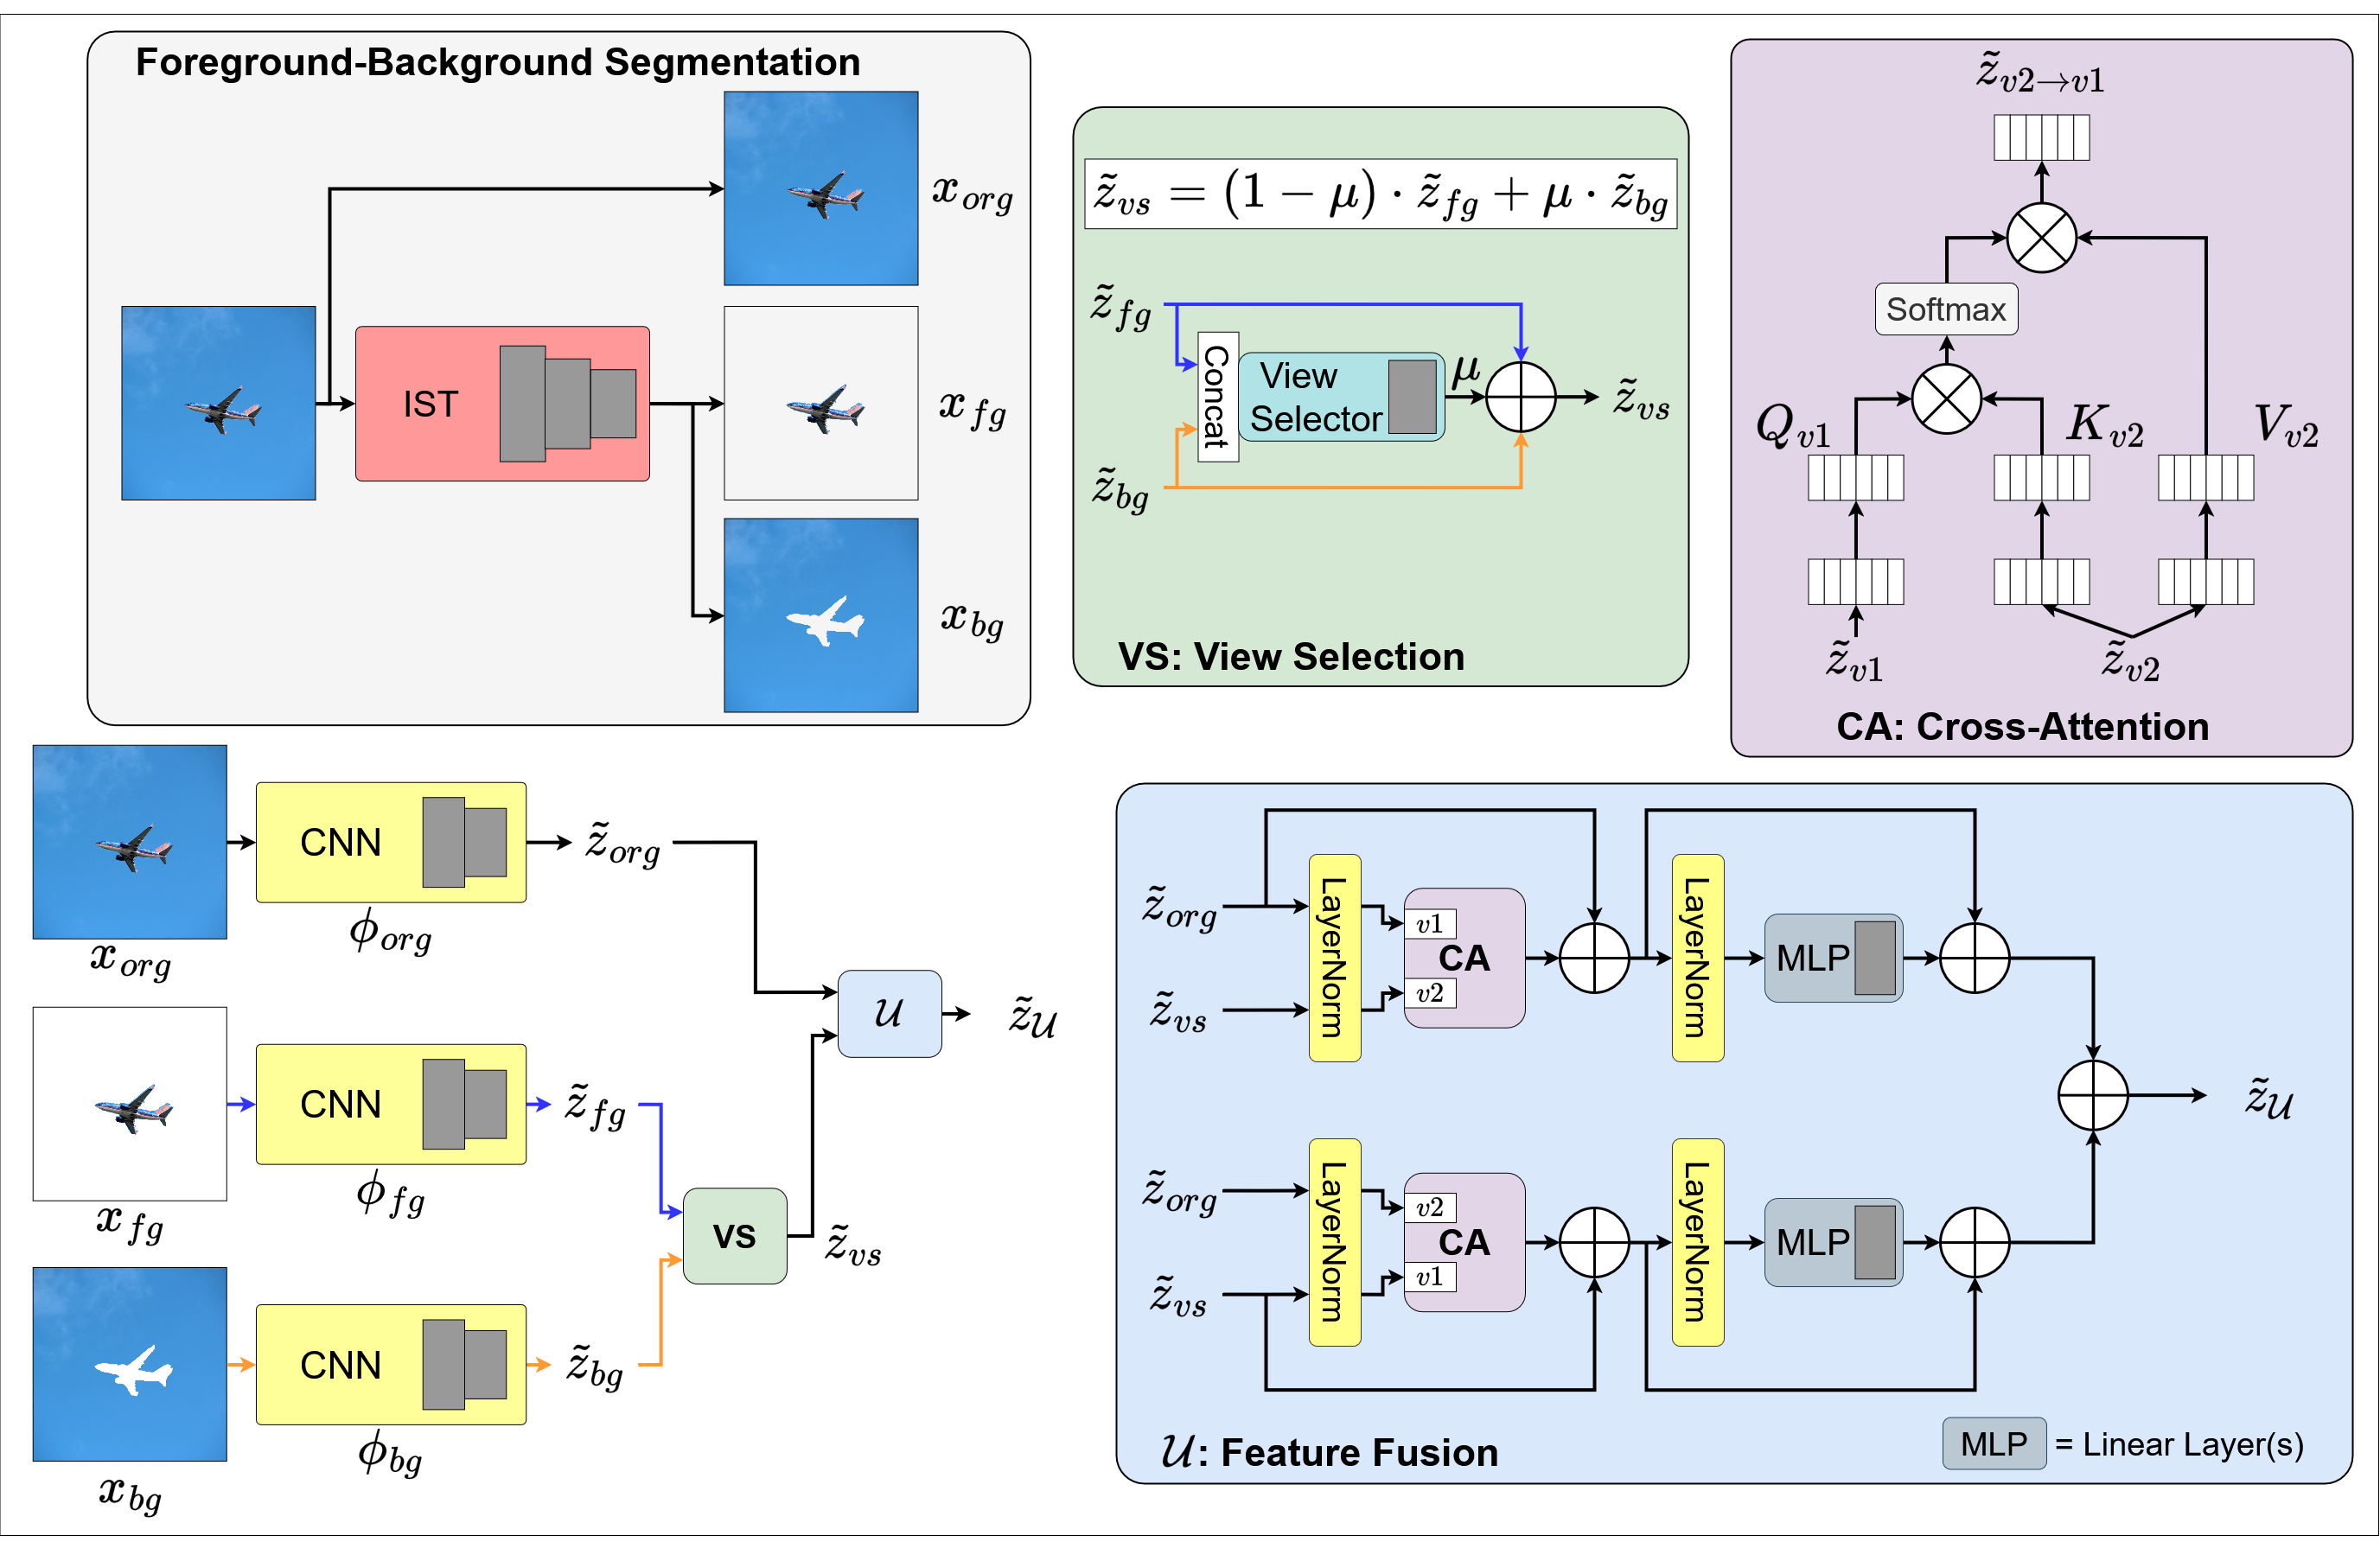
\includegraphics[width=1.\linewidth]{figures/scod_diagram}
  \caption{Model architecture of the proposed \sysc. %Foreground-background segmentation was done on entire datasets during setup. Black lines refer to the original or fused image features. Blue lines refer to foreground image features, orange lines refer to background image features.
  }
\label{fig:propwork-scod-diagram}
\end{figure*}

%\sysb resembles \sysa in that a MVCNN is used for the FgBg multi-view model $f_{MV}$ backbone. Each feature extractor $\phi_v = f_{\theta,v}$ (parameterized by $\theta$) outputs a $d$-dimensional feature vector from input view $x_v$, $\phi_v: \mathcal{X} \mapsto \mathbb{R}^d$. The multi-view feature extractors $\phi_{MV}$ give $Z_{MV} = \{z_{org}, z_{fg}, z_{bg}\}$ with corresponding classification parameters $W_{MV}$ and $b_{MV}$ subsequently outputting $\hat{Y}_{MV} = \{\hat{y}_{org}, \hat{y}_{fg}, \hat{y}_{bg}\}$. The fusion component $\mathcal{U}$ in \sysb differs significantly from \sysa, instead constructing the single-view features, cross-view features, and comprehensive fused feature for ensembling.
The structure of SCOD is similar to that of MOD and MEO. An MVCNN is used as the backbone for the FgBg multi-view model $f_{MV}$, with multi-view feature extractors $\phi_v = f_{\theta,v}$, parameterized by $\theta$, taking as input views $x_v$ and providing as output view features $\tilde{z}_v = \phi_v (x_v)$. Note, however, that in SCOD, view features are extracted \textbf{prior to the average-pooling and flattening operations} (and thus are not vectors). That is, $\phi_v: \mathcal{X} \mapsto \mathbb{R}^{\mathcal{I} \times \mathcal{J} \times \mathcal{K}}$, where $\mathcal{I}$ is the image convolution channel dimension, $\mathcal{J}$ is the image convolution width dimension, and $\mathcal{K}$ is the image convolution height dimension. Feature vectors are computed by applying average-pooling and flattening operations to features, $z_v = flat(\text{AvgPool}(\tilde{z}_v))$, where $flat(\cdot)$ is a matrix-flattening operation converting from $\mathbb{R}^{\mathcal{I} \times 1 \times 1}$ to $\mathbb{R}^{\mathcal{I}}$ and $\text{AvgPool}$ is an average-pooling operation across dimension $\mathcal{J} \times \mathcal{K}$ (collapsing $\mathbb{R}^{\mathcal{I} \times \mathcal{J} \times \mathcal{K}}$ to $\mathbb{R}^{\mathcal{I} \times 1 \times 1}$). For SCOD, $f_{MV}$ outputs multi-view features $\tilde{Z}_{MV} = \{\tilde{z}_{org}, \tilde{z}_{fg}, \tilde{z}_{bg}\}$ and feature vectors $Z_{MV} = \{z_{org}, z_{fg}, z_{bg}\}$. Individual classification parameters $W_{MV}$, $b_{MV}$ take as input $Z_{MV}$ and output prediction logits $\hat{Y}_{MV} = \{\hat{y}_{org}, \hat{y}_{fg}, \hat{y}_{bg}\}$. The fusion component $\mathcal{U}$ for SCOD uses the view selector from MOD but dramatically upgrades the feature fusion computation by introducing the usage of Transformer-inspired \emph{cross-attention} \cite{vaswani2017attention}.

%The diagram in Figure \ref{fig:propwork-mod-diagram} illustrates the high-level operations and flow of information in \sysa. An IST segments an image into a foreground view and a background view. The MVCNN architecture converts the input original image view (\textit{org}), foreground view (\textit{fg}), and background view (\textit{bg}) to view-specific feature vectors $Z_{MV} = \{z_{org}, z_{fg}, z_{bg}\}$. Each feature extractor $\phi_v$ in \sysa is implemented with a ResNet-18 \cite{he2016deep} model. Of note, however, is that the design of \sysa is modular. Any model capable of processing an input image and outputting a feature vector $z_v \in \mathbb{R}^d$ is compatible. The fusion component in \sysa $\mathcal{U}_{\text{\sysa}}$ uses \emph{view selection} to combine information in $Z_{MV}$ into a fused feature vector $z_{\mathcal{U}} = \mathcal{U}_{\text{\sysa}}(Z_{MV})$, $z_{\mathcal{U}} \in \mathbb{R}^d$.
%The flow of information for \sysb is illustrated in Figure \ref{fig:propwork-meo-diagram}. The IST segments the original image view (\textit{org}) into a foreground view (\textit{fg}) and a background view (\textit{bg}). The MVCNN backbone generates features $Z_{MV}$ and logits $\hat{Y}_{MV}$. In \sysb, the fusion component $\mathcal{U}$ is composed of three modules.
The information flow for SCOD is presented in \ref{fig:propwork-scod-diagram} and follows that of MOD closely, with the IST segmenting the original image view (\textit{org}) into foreground (\textit{fg}) and background (\textit{bg}) views, the MVCNN backbone generating features $\tilde{Z}_{MV}$, feature vectors $Z_{MV}$, and logits $\hat{Y}_{MV}$ from the views, and the fusion component $\mathcal{U}_{\text{\sysc}}$ combining view information into fused feature $\tilde{z}_{\mathcal{U}}$. Notably, $\mathcal{U}_{\text{\sysc}}$ differs from MOD in the fusion mechanisms after view selection. Overlapping details are not mentioned in this section and instead should be assumed to mimic those in Section \ref{sec:propwork-mod-propmeth}.

%\textbf{View Selector:} The view selector is implemented using a fully connected layer $f_{\theta}$ that takes the concatenation of average-pooled and flattened foreground and background features $[z_{fg,flat}; z_{bg,flat}] \in \mathbb{R}^{2C}$ as inputs and outputs a view selection weight $s$
%\begin{equation}
%\begin{split}
%    z_{fg,flat} & = flat(\text{AvgPool}(z_{fg})) \in \mathbb{R}^{C} \\
%    z_{bg,flat} & = flat(\text{AvgPool}(z_{bg})) \in \mathbb{R}^{C} \\
%    s & = \sigma (f_{\theta}([z_{fg,flat}; z_{bg,flat}]))
%\end{split}
%\end{equation}
%where $flat(\cdot)$ is a matrix-flattening operation converting from $\mathbb{R}^{C \times 1 \times 1}$ to $\mathbb{R}^{C}$, $\text{AvgPool}$ is an average-pooling operation across dimensions $H \times W$ (collapsing $\mathbb{R}^{C \times H \times W}$ to $\mathbb{R}^{C \times 1 \times 1}$), and $\sigma$ is the sigmoid function.~Note,~the view selector is class-agnostic.~The original view feature $z_{org}$ does not take part in view selection as it contains overall semantic information. We always include it in feature fusion. The view selector features $z_{vs}$ is the sum of $z_{fg}$ and $z_{bg}$ weighted by $s$
%\begin{equation}
%     z_{vs} = (1 - s) \cdot z_{fg} + s \cdot z_{bg}
%\end{equation}
\subsubsection{View Selector}
The view selection operation in SCOD is identical to that in MOD. It takes as input the foreground and background view-specific feature vectors $z_{fg}, z_{bg}$ and produces as output the view selection weight $\mu$. See Section \ref{sec:propwork-mod-propmeth} for details.

%\textbf{Feature Fusion:} The view selection feature $z_{vs}$ contains the ID class-relevant feature information between the foreground and background views. This information is complementary to the feature information in $z_{org}$. %and can identify critical feature information across views useful for identifying ID image classes. 
%Cross-attention allows models to focus on class-relevant discriminative information in images represented across different views via attention weights learned using features from both views \cite{tsai2019multimodal,wang2024mutualformer,lee2024crossformer}. As such, we use a cross-attention architecture to learn these cross-view complementary features from the original view and the selected view.%, inspired by previous work using cross-attention techniques \cite{tsai2019multimodal,wang2024mutualformer,lee2024crossformer}.} %In our proposed cross-attention feature fusion module, we introduce a \textit{cross-view correlation} operation that explicitly encourages alignment between the original feature and view selection feature for greater informative transfer and discriminative feature learning.
%
%The cross-attention feature fusion module receives as input $z_{org}$ and $z_{vs}$. Both features are reshaped from $\mathbb{R}^{C \times H \times W}$ to $\mathbb{R}^{T \times d}$. $T$ is the sequence length resulting from dividing the spatial dimensions into tokens and appending a class token, i.e. $T = 1 + H \times W$. $d$ is the channel information of the feature, i.e. $d = C$. We also add position encodings to $z_{org}$ and $z_{vs}$.
%
%The fusion module is composed of two branches, one a reflection of the other. Without loss of generality, we represent the inputs to a branch as $z_{v1}$ and $z_{v2}$. A branch takes $z_{v1}$ and $z_{v2}$ and extracts queries $Q = FF_{Q}(LN(z_{v1})) \in \mathbb{R}^{T_{v1} \times d_{k}}$ from $z_{v1} \in \mathbb{R}^{T_{v1} \times d_{v1}}$ using feed-forward layer $FF_{Q}$ ($LN$ is the LayerNorm operation), and keys $K = FF_{K}(LN(z_{v2})) \in \mathbb{R}^{T_{v1} \times d_{k}}$ and values $V = FF_{V}(LN(z_{v2})) \in \mathbb{R}^{T_{v1} \times d_{w}}$ from $z_{v2}$ using feed-forward layers $FF_{K}$ and $FF_{V}$. These queries, keys, and values are then used to generate the cross-attention features $z_{v2 \rightarrow v1}$
%%The cross-attention feature fusion module receives as input the original view convolutional features $z_{org} \in \mathbb{R}^{T_{org} \times d_{org}}$ from the penultimate layer of the original view feature extractor $\phi_{org}$ and the view selection features $z_{vs} \in \mathbb{R}^{T_{vs} \times d_{vs}}$. $T_{(\cdot)}$ is the sequence length and $d_{(\cdot)}$ is the feature dimension. (Note that we follow the Transformer format and append a class token to the convolutional dimension i.e. $T = 1 + C$ for a convolutional feature $z_{conv} \in \mathbb{R}^{C \times d}$.) The fusion module is composed of two branches, one a reflection of the other. Without loss of generality, we represent the inputs to a branch as $z_{v1}$ and $z_{v2}$. A branch takes $z_{v1}$ and $z_{v2}$ and extracts queries $Q = FF_{Q}(z_{v1})$ from $z_{v1}$ using feed-forward layer $FF_{Q}$ taking as input dimensionality $d_{org}$ and yielding dimensionality $d_{k}$, and keys $K = FF_{K}(z_{v2})$ and values $V = FF_{V}(z_{v2})$ from $z_{v2}$. These queries, keys, and values are then used to generate the cross-attention features $z_{v2 \rightarrow v1}$
%\begin{equation}
%\begin{split}
%     z_{v2 \rightarrow v1} & = CAF_{v2 \rightarrow v1}(LN(z_{v1}), LN(z_{v2})) 
%     %\\ & 
%     = \text{softmax} \left( \frac{Q K^{\mathsf{T}}}{\sqrt{d_{k}}} \right) V
%\end{split}
%\end{equation}
%%The two branches result in two cross-attention features $z_{vs \rightarrow org}$ and $z_{org \rightarrow vs}$. We propose a novel cross-view correlation that enhances the aligned information across both views
%%\begin{equation}
%%    z_{v2 \rightarrow v1, enh} = \epsilon \cdot z_{v2 \rightarrow v1} + (1 - \epsilon) \cdot z_{v1 \rightarrow v2}
%%\end{equation}
%%where $\epsilon$ is a correlation balance hyperparameter. 
%The final resultant feature for a branch $S_{v2 \rightarrow v1}$ is summarized below
%\begin{equation}
%\begin{split}
%    %\hat{S}_{v2 \rightarrow v1} = \epsilon \cdot CAF_{v2 \rightarrow v1}(LN(z_{v1}), LN(z_{v2})) + (1 - \epsilon) \cdot CAF_{v1 \rightarrow v2}(LN(z_{v2}), LN(z_{v1})) + z_{v1} \\
%    %= z_{v2 \rightarrow v1, enh} + z_{v1} \\
%    %\hat{S}_{v2 \rightarrow v1} & =  z_{v2 \rightarrow v1, enh} + z_{v1} \\
%    \hat{S}_{v2 \rightarrow v1} & =  z_{v2 \rightarrow v1} + z_{v1} \\
%    S_{v2 \rightarrow v1} & = f_{\psi_{v2 \rightarrow v1}} (LN(\hat{S}_{v2 \rightarrow v1})) + \hat{S}_{v2 \rightarrow v1}
%\end{split}
%\end{equation}
%where $f_{\psi}$ is a linear layer parameterized by $\psi$.
%The final fused feature is an element-wise sum of the two branch features. Here we replace $v1$ and $v2$ with appropriate $org$ and $vs$
%\begin{equation}
%    z_{fused} = S_{vs \rightarrow org} + S_{org \rightarrow vs}
%\end{equation}
\subsubsection{Fusion Component}
For SCOD, the fusion component $\mathcal{U}_{\text{\sysc}}$ uses the view selection weight $\mu$ and \emph{cross-attention} to fuse correlated feature information across views and compute the fused feature $\tilde{z}_{\mathcal{U}}$. The view selector feature $\tilde{z}_{vs}$ is the sum of $\tilde{z}_{fg}$ and $\tilde{z}_{bg}$ weighted by $\mu$
\begin{equation}
\begin{aligned}
     \tilde{z}_{vs} = (1 - \mu) \cdot \tilde{z}_{fg} + \mu \cdot \tilde{z}_{bg}.
\end{aligned}
\end{equation}
The view selector feature $\tilde{z}_{vs}$ contains ID class-relevant feature information between the foreground and background views according to learned knowledge (from the defined optimization, see Section \ref{sec:propwork-mod-propmeth}). This information is complementary to the feature information in $\tilde{z}_{org}$.

Cross-attention allows models to focus on class-relevant discriminative information in images represented across different views via attention weights learned using features from both views \cite{tsai2019multimodal,wang2024mutualformer,lee2024crossformer}. As such, a cross-attention architecture is used to learn these cross-view complementary features from the original view and the selected view. The cross-attention feature fusion module generally follows the formulation described in Section \ref{sec:bkgd-attn}. It receives as input $\tilde{z}_{org}$ and $\tilde{z}_{vs}$. Both features are reshaped from $\mathbb{R}^{\mathcal{I} \times \mathcal{J} \times \mathcal{K}}$ to $\mathbb{R}^{T \times d}$. $T$ is the sequence length resulting from dividing the spatial dimensions into tokens and appending a class token, i.e. $T = 1 + \mathcal{J} \times \mathcal{K}$. $d$ is the channel information of the feature, i.e. $d = \mathcal{I}$. Position encodings are also added to $\tilde{z}_{org}$ and $\tilde{z}_{vs}$.

The fusion module is composed of two branches, one a reflection of the other. Without loss of generality, the inputs to a branch are represented as $\tilde{z}_{v1}$ and $\tilde{z}_{v2}$. A branch takes $\tilde{z}_{v1}$ and $\tilde{z}_{v2}$ and extracts queries $Q$, keys $K$, and values $V$ via
\begin{equation}
\begin{aligned}
    Q & = W_Q LN(\tilde{z}_{v1}; \gamma_{1,q}, \beta_{1,q}) \\
    K & = W_K LN(\tilde{z}_{v2}; \gamma_{1,k}, \beta_{1,k}) \\
    V & = W_V LN(\tilde{z}_{v2}; \gamma_{1,v}, \beta_{1,v}). \\
\end{aligned}
\end{equation}
$W_Q \in \mathbb{R}^{T_{v1} \times d_k}$, $W_K \in \mathbb{R}^{T_{v2} \times d_k}$, $W_V \in \mathbb{R}^{T_{v2} \times d_v}$ are weight matrices and $LN$ is the LayerNorm operation \cite{xu2019understanding}
\begin{equation}
\begin{aligned}
    & LN(\tilde{z}; \gamma, \beta) = \gamma \frac{(\tilde{z} - \mu_{\tilde{z}})}{\sigma_{\tilde{z}}} + \beta \\
    & \mu_{\tilde{z}} = \frac{1}{k} \sum_{i=1}^{k} \tilde{z}_i,\ \sigma_{\tilde{z}} = \sqrt{\frac{1}{k} \sum_{i=1}^{k} (\tilde{z}_i - \mu_{\tilde{z}})^2}.
\end{aligned}
\end{equation}
In SCOD, $T_{v1} = T_{v2} = T$ and $d_k = d_v = d$.
Note that the two branches are not identical. In one branch, $v1$ is used to compute $Q$ while $v2$ is used to compute $K$ and $V$. In the other branch, the association is swapped, $v2$ is used to compute $Q$ while $v1$ is used to compute $K$ and $V$. This dual-branch configuration ensures that each input feature has a chance to attend to the other, providing a comprehensive reinforcement of discriminative features across views.
The queries $Q$, keys $K$, and values $V$ are used to generate the cross-attention features $\tilde{z}_{v2 \rightarrow v1}$
\begin{equation}
\begin{split}
     \tilde{z}_{v2 \rightarrow v1} & = CAF_{v2 \rightarrow v1}(LN(\tilde{z}_{v1}), LN(\tilde{z}_{v2})) 
     %\\ & 
     = \text{softmax} \left( \frac{Q K^{\mathsf{T}}}{\sqrt{d_{k}}} \right) V.
\end{split}
\end{equation}

The final resultant feature for a branch $S_{v2 \rightarrow v1}$ is summarized below
\begin{equation}
\begin{split}
    \hat{S}_{v2 \rightarrow v1} & =  \tilde{z}_{v2 \rightarrow v1} + \tilde{z}_{v1} \\
    S_{v2 \rightarrow v1} & = (W_{v2 \rightarrow v1,2}\ \text{ReLU}(W_{v2 \rightarrow v1,1} (LN(\hat{S}_{v2 \rightarrow v1}); \gamma_2, \beta_2) + b_{v2 \rightarrow v1,1}) + b_{v2 \rightarrow v1,2}) + \hat{S}_{v2 \rightarrow v1}
\end{split}
\end{equation}
where $W_{v2 \rightarrow v1,1} \in \mathbb{R}^{d \times \kappa}, W_{v2 \rightarrow v1,2} \in \mathbb{R}^{\kappa \times d}$ are weight matrices and $b_{v2 \rightarrow v1,1} \in \mathbb{R}^{d}, b_{v2 \rightarrow v1,2} \in \mathbb{R}^{d}$ are biases for the feature resulting from attention operations (per the proven methodology in Transformer architectures \cite{vaswani2017attention}). $ReLU$ is the Rectified Linear Unit activation function \cite{ramachandran2017searching}. $\kappa$ is a hyperparameter.
The final fused feature is an element-wise sum of the two branch features. Here, $v1$ and $v2$ are replaced with the appropriate $org$ and $vs$
\begin{equation}
    \tilde{z}_{\mathcal{U}} = S_{vs \rightarrow org} + S_{org \rightarrow vs}.
\end{equation}
For downstream tasks, the class token of the final fused feature $z_{\mathcal{U}} = \tilde{z}_{\mathcal{U}}^{0}$ is used.

%\textbf{Fusion Prediction and Detection:} The class token of the fused feature $z_{fused}$ is used for OoD scoring (see Section \ref{sec:method-ood}). View-specific feature $z_{org}$, $z_{fg}$, $z_{bg}$ are not used because they are learned from limited information, degrading their OoD detection capability (see Section \ref{sec:disc} for details). Individual linear layers are used with the fused and view-specific feature vectors to produce fused prediction logits $\hat{y}_{fused}$ and view-specific prediction logits $\hat{y}_{org}$, $\hat{y}_{fg}$, $\hat{y}_{bg}$.
\subsubsection{Prediction} 
Similar to MOD and MEO, the fused feature vector and view-specific feature vectors,
\begin{equation}
\begin{aligned}
    z_{org} & = \tilde{z}_{org}^{0} \\
    z_{fg} & = \tilde{z}_{fg}^{0} \\
    z_{bg} & = \tilde{z}_{bg}^{0},
\end{aligned}
\end{equation}
are used for prediction. Individual linear layers with weight matrices $W_{\mathcal{U}}, W_{MV}$ and biases $b_{\mathcal{U}}, b_{MV}$ are used with the fused and view-specific feature vectors respectively to produce fused prediction logits $\hat{y}_{\mathcal{U}}$ and view-specific prediction logits $\hat{y}_{org}$, $\hat{y}_{fg}$, $\hat{y}_{bg}$.

%\sys is designed around two components: the feature extractors and the view selector. We choose to train \sys using an alternating-objectives paradigm as it is more effective for modular architectures (like ours) compared to end-to-end learning \cite{shalev2017failures,glasmachers2017limits,pascal2021improved,liu2023convergence}. The first training objective is a combination of the classification loss $\mathcal{L}_{CE}$ and alignment loss $\mathcal{L}_{con}$ for feature extraction, and the second training objective is the view selection loss $\mathcal{L}_{VS}$.
\subsubsection{Training}
The design of SCOD mimics that of MOD and a similar, alternating optimization paradigm is used. Training objectives are targeted towards the feature extractors and the fusion component. The fusion component loss $\mathcal{L}_{VS}$ is similar to MOD and targets learning of the view selector. However, the feature extraction objective improves on MOD by introducing an alignment loss $\mathcal{L}_{con}$ in addition to the classification loss $\mathcal{L}_{CE}$.

%$\mathcal{L}_{CE}$ is formulated as follows.~For each view $v \in \{org, fg, bg\}$, we first define a view-specific CE loss $\mathcal{L}_{CE,v}$
%\begin{equation}
%\begin{aligned}
%    \mathcal{L}_{CE,v}(y, \hat{y}_v) & = -\sum_{c \in \mathcal{Y}} y_{c} \log(\hat{y}_{v,c}) \\
%\end{aligned}
%\end{equation}
%where $\hat{y}_{v,c}$ denotes the logit value of $\hat{y}_{v}$ for class $c$ and $y$ is the one-hot true label vector. We also create another CE loss involving the fused prediction logits, as given by
%\begin{equation}
%\begin{aligned}
%    \mathcal{L}_{CE,fused}(y, \hat{y}_{fused}) & = -\sum_{c \in \mathcal{Y}} y_{c} \log(\hat{y}_{fused,c}) \\
%\end{aligned}
%\end{equation}
%where $\hat{y}_{fused,c}$ is the logit value of $\hat{y}_{fused}$ for class $c$. The final CE loss $\mathcal{L}_{CE}$ is the combination of the four losses
%\begin{equation}
%\begin{aligned}
%    %\mathcal{L}_{CE} & = \sum_{v ~\in~ \{fused, ~org, ~fg, ~bg\}} \mathcal{L}_{CE,v} (y, \hat{y}_{v})\\
%    \mathcal{L}_{CE} ~= ~\smashoperator{\sum_{v \in \{fused, ~org, ~fg, ~bg\}}} \mathcal{L}_{CE,v} (y, \hat{y}_{v})
%\end{aligned}
%\end{equation}
$\mathcal{L}_{CE}$ is formulated as follows. For each view $v \in \{org, fg, bg\}$, a view-specific CE loss $\mathcal{L}_{CE,v}$ is defined as
\begin{equation}
\begin{aligned}
    \mathcal{L}_{CE,v}(y, \hat{y}_v) & = -\sum_{c \in \mathcal{Y}} y_{c} \log(\hat{y}_{v,c}). \\
\end{aligned}
\end{equation}
Another CE loss involving the fused prediction logits is defined as
\begin{equation}
\begin{aligned}
    \mathcal{L}_{CE,\mathcal{U}}(y, \hat{y}_{\mathcal{U}}) & = -\sum_{c \in \mathcal{Y}} y_{c} \log(\hat{y}_{\mathcal{U},c}). \\
\end{aligned}
\end{equation}
The final CE loss $\mathcal{L}_{CE}$ is the combination of the four losses
\begin{equation}
\begin{aligned}
    \mathcal{L}_{CE} ~= ~\smashoperator{\sum_{v \in \{\mathcal{U}, ~org, ~fg, ~bg\}}} \mathcal{L}_{CE,v} (y, \hat{y}_{v}).
\end{aligned}
\end{equation}

It has been found that including contrastive losses can help improve alignment of features from different views and modalities \cite{karpathy2014deep,ke2024rethinking,li2021rfn,ding2022cooperative}. This observation is leveraged in the updated objectives for SCOD by including an alignment loss that pushes $(\tilde{z}_{org}, \tilde{z}_{fg})$ and $(\tilde{z}_{org}, \tilde{z}_{bg})$ towards greater similarity \cite{ding2022cooperative,wang2023connecting,liang2022mind}. However, $\tilde{z}_{fg}$ and $\tilde{z}_{bg}$ likely contain orthogonal information as the pixel information in their images are mutually exclusive. Thus, to encourage greater feature diversity, a term is introduced that pushes $(\tilde{z}_{fg}, \tilde{z}_{bg})$ towards \textit{dissimilarity}. The contraction term of contrastive losses is used to encourage alignment while the negative of the contraction term is used to encourage misalignment (i.e. maximally orthogonal alignment)
\begin{equation}
    \mathcal{L}_{con} = -sim(\tilde{z}_{org}, \tilde{z}_{fg})/\tau_{of} - sim(\tilde{z}_{org}, \tilde{z}_{bg})/\tau_{ob} + \gamma sim(\tilde{z}_{fg}, \tilde{z}_{bg})/\tau_{fb},
\end{equation}
where $\tau_{(\cdot)}$ are temperature hyperparameters, $\gamma$ is a misalignment weight hyperparameter, and $sim(\cdot,\cdot)$ is the cosine similarity function \cite{xia2015learning}.

%\textbf{View Selection Loss:} Given view-specific prediction logits $\hat{y}_v$ ($v \in \{fg,~bg\}$), low classification error using $\hat{y}_v$ implies that the corresponding view feature $z_{v}$ (and view $v$) has encoded more informative discriminative features to help classification. Based on this idea, we construct a view selection loss $\mathcal{L}_{VS}$ that guides the view selector (Section \ref{sec:method-rep}) to learn and adjust $s$ towards including more of either the foreground or the background view via soft-weighting, minimizing the classification error and improving OoD detection ability. Note that this method does not use any external supervision.
%\begin{equation}
%\begin{aligned}
%    E_{fg} = \text{RMSE}(\hat{y}_{fg}, y) \\
%    E_{bg} = \text{RMSE}(\hat{y}_{bg}, y) \\
%    s' = \sigma(\tanh(E_{fg}) - \tanh(E_{bg})) \\
%    \mathcal{L}_{VS} = \beta ~\text{MSE}(s, s')
%\end{aligned}
%\end{equation}
%where $E_{fg}$ and $E_{bg}$ are the Root Mean Square Errors (RMSE) corresponding to $\hat{y}_{fg}$ and $\hat{y}_{bg}$; $s'$ is the target view selection weight which is set to select the view with less classification error (i.e. $0$ for foreground and $1$ for background) during training; %$\psi$ is a scaling factor hyper-parameter and 
%$\beta$ is a regularization hyper-parameter. %$\psi$ is particularly noteworthy as it serves to sharpen the sigmoid function and thus, approximates $s$ as a hard gate. 
The view selection loss $\mathcal{L}_{VS}$ in SCOD is identical to that in MOD
\begin{equation}
\begin{aligned}
    E_{fg} = \text{RMSE}(\hat{y}_{fg}, y) \\
    E_{bg} = \text{RMSE}(\hat{y}_{bg}, y) \\
    \mu' = \sigma(\psi(\tanh(E_{fg}) - \tanh(E_{bg}))) \\
    \mathcal{L}_{VS} = \delta ~\text{MSE}(\mu, \mu').
\end{aligned}
\end{equation}

%In the first phase, \sys is trained with $\mathcal{L}_{CE} + \mathcal{L}_{con}$ for some number of epochs, while the view selector parameters are kept frozen. In the second phase, the view selector parameters are unfrozen while the rest of the model parameters are frozen, and the view selector is trained with $\mathcal{L}_{VS}$ for some number of epochs. This cycle repeats until both losses are converged.
As in MOD, SCOD is trained in two alternating phases. In the first phase, SCOD is trained with $\mathcal{L}_{CE} + \mathcal{L}_{con}$ for a predetermined number of epochs. During this time, the view selector parameters are kept frozen. In the second phase, the view selector parameters are unfrozen while the rest of the model parameters are frozen, and the view selector is trained with $\mathcal{L}_{VS}$ for another predetermined number of epochs. This cycle repeats until both losses converge or some maximum number of epochs has passed.

%\textbf{Testing:} At test time, each test sample is processed in the same way as each training sample: segmentation and feeding the three views to the system. 
\subsubsection{OOD Detection}
SCOD follows MOD in that only $z_{\mathcal{U}}$ and $\hat{y}_{\mathcal{U}}$ are used for OOD detection. See Section \ref{sec:propwork-mod-propmeth} for details.

\subsection{Experiments}
\label{sec:propwork-scod-exp}

The experimental setup for SCOD uses the same datasets, image segmentation model, feature extractor architecture, baselines, and evaluation metrics as those in MOD. The training details differ due to the introduction of a contrastive loss term to the optimization objective. Training settings are:
\begin{itemize}
    \item Batch Size = 64
    \item Epochs = 400 or until convergence
    \item Optimizer = ADAM \cite{zhang2018improved}
    \item Learning Rate = 5e-4
    \item Cosine Annealing (across all epochs)
\end{itemize}
A grid search was likewise performed for SCOD over hyperparameters $\psi$ (50 to 300, intervals of 50), $\delta$ (50 to 200, intervals of 50), and $\gamma$ (0.5 to 2.0, intervals of 0.25). All were set to the optimal found value: $\psi$ was set to 200, $\delta$ was set to 100, and $\gamma$ was set to 1.75. The training periods were set to those used in MOD. All temperature hyperparameters $\tau$ terms are $1$. All other hyperparameters were set to the default value (e.g. architectural hyperparameters).

\subsection{Results}
\label{sec:propwork-scod-results}

\begin{table*}[h!]
\small
\centering
\caption{CIFAR-10 ID classification (\textbf{Accuracy}) and OOD detection performance (\textbf{AUC}) comparison between \sysc, \sysa, and recent state-of-the-art baselines. %All numeric values are percentages. Best results are emphasized with \textbf{boldface}. 
%Near-OOD datasets are marked with ``*'' and unavailable results with ``/''. ``Far'' refers to the average AUC performance across far-OOD datasets, ``Near'' refers to the average AUC performance across near-OOD datasets, and ``Avg.'' refers to the cumulative average AUC performance across all OOD datasets.
}
\vspace{0.1cm}
\scalebox{0.73}{
\begin{tabular}{|l|c|cccccc|ccc|}
\hline
\multicolumn{1}{|l|}{\multirow{2}{*}{}} & ID   & \multicolumn{9}{c|}{OOD}  \\ \cline{2-11} 
\multicolumn{1}{|l|}{}  & C10 & C100*  & LSUN   & TXT & Places & iNat & TIN* & \multicolumn{1}{|c}{Far} & Near & \multicolumn{1}{c|}{Avg.} \\ \hline
MSP   & 94.73$_{\pm 0.11}$   & 87.05$_{\pm 0.51}$   &  90.45$_{\pm 0.42}$   & 92.01$_{\pm 0.58}$   & 89.88$_{\pm 0.55}$   & 90.20$_{\pm 0.73}$   & \multicolumn{1}{c|}{87.98$_{\pm 0.34}$} & 90.63 & 87.51  & 89.59  \\  
KNN   & 94.73$_{\pm 0.11}$   & 89.55$_{\pm 0.22}$   & 92.29$_{\pm 0.15}$   & 94.24$_{\pm 0.40}$   & 91.46$_{\pm 0.25}$   & 91.73$_{\pm 0.62}$   & \multicolumn{1}{c|}{90.15$_{\pm 0.14}$}  & 92.43 & 89.85   &  91.57   \\ 
MD    & \textbf{95.37}$_{\pm 0.13}$   & 88.85$_{\pm 0.21}$   &  90.98$_{\pm 0.25}$   & 95.67$_{\pm 0.23}$   & 90.37$_{\pm 0.26}$   & 91.85$_{\pm 0.69}$   & \multicolumn{1}{c|}{89.08$_{\pm 0.18}$} & 92.22 & 88.96    &   91.13   \\  
ViM   & 94.73$_{\pm 0.11}$   & 86.39$_{\pm 1.72}$   & 89.26$_{\pm 2.05}$   & 96.05$_{\pm 1.04}$   & 88.05$_{\pm 1.96}$   & 89.96$_{\pm 1.27}$   & \multicolumn{1}{c|}{87.26$_{\pm 1.56}$}  & 90.83 & 86.82   &   89.49   \\  
React & 94.73$_{\pm 0.11}$   & 84.82$_{\pm 1.39}$   & 91.47$_{\pm 0.55}$   & 90.67$_{\pm 0.89}$   & 89.57$_{\pm 1.11}$   & 87.94$_{\pm 2.30}$   & \multicolumn{1}{c|}{86.76$_{\pm 0.98}$}  & 89.91 & 85.79   &   88.54  \\  
FeatNorm & 94.73$_{\pm 0.11}$ & 88.89$_{\pm 0.66}$  &  91.93$_{\pm 1.15}$   & 94.61$_{\pm 0.23}$   & 95.37$_{\pm 0.41}$   & 94.14$_{\pm 1.31}$   & \multicolumn{1}{c|}{90.16$_{\pm 0.81}$}  & 94.01 & 89.53  &   92.52   \\ 
GEN   & 94.73$_{\pm 0.11}$   & 87.19$_{\pm 0.58}$   &  91.35$_{\pm 0.53}$   & 92.53$_{\pm 0.79}$   & 90.82$_{\pm 0.65}$   & 90.97$_{\pm 0.90}$   & \multicolumn{1}{c|}{88.56$_{\pm 0.40}$} & 91.42 & 87.87   &   90.24  \\  
LogitNorm & 94.56$_{\pm 0.22}$ & 90.80$_{\pm 0.82}$ & 95.06$_{\pm 0.59}$   & 94.53$_{\pm 1.07}$   & 95.66$_{\pm 0.42}$   & 93.18$_{\pm 1.05}$   & \multicolumn{1}{c|}{91.80$_{\pm 0.65}$} & 94.61 & 91.30   &   93.51   \\ 
CSI  & / & 92.2$_{\pm 0.1}$     & \textbf{97.7}$_{\pm 0.4}$  & /  & /   & /   & \multicolumn{1}{c|}{\textbf{97.6}$_{\pm 0.3}$} & / & 94.90 &  /  \\  
CMG-e   & /   & 89.3$_{\pm 0.4}$   & \textbf{97.7}$_{\pm 0.9}$  & / & /  & / & \multicolumn{1}{c|}{95.2$_{\pm 2.7}$}  & / & 92.25 &    /      \\  \hline
MOD-MD  & \textbf{95.37}$_{\pm 0.29}$ & \textbf{95.54}$_{\pm 5.39}$ & 96.02$_{\pm 2.97}$ & \textbf{98.42}$_{\pm 1.12}$ & 95.90$_{\pm 3.04}$ & \textbf{98.63}$_{\pm 0.57}$ & \multicolumn{1}{c|}{96.34$_{\pm 2.60}$}  & \textbf{97.24} & \textbf{95.94}  & \textbf{96.81}   \\ %\hline
MOD-KNN  & \textbf{95.37}$_{\pm 0.29}$ & 95.10$_{\pm 3.73}$ & 97.37$_{\pm 1.13}$ & 97.56$_{\pm 1.17}$ & \textbf{96.48}$_{\pm 1.37}$ & 97.41$_{\pm 1.14}$ & \multicolumn{1}{c|}{96.39$_{\pm 0.91}$} & 97.21 & 95.74  &  96.72  \\ \hline
SCOD-MD  & 94.37$_{\pm 0.33}$ &  94.19$_{\pm 1.80}$ & 96.72$_{\pm 0.81}$ & 95.48$_{\pm 1.06}$ & 96.26$_{\pm 1.28}$ & 98.17$_{\pm 0.95}$ & 95.76$_{\pm 0.76}$  & 96.66 & 94.98 &  96.10     \\ 
SCOD-KNN  & 94.37$_{\pm 0.33}$ & 92.00$_{\pm 1.55}$ & 95.00$_{\pm 0.41}$ & 94.61$_{\pm 1.18}$ & 93.46$_{\pm 0.67}$ & 97.12$_{\pm 1.39}$ & 94.04$_{\pm 1.36}$ & 95.05 & 93.02 &  94.37   \\ \hline
\end{tabular}
}
\label{tab:propwork-scod-results-cifar10}
\end{table*}

\begin{table*}[h!]
\small
\centering
\caption{CIFAR-100 ID classification (\textbf{Accuracy}) and OOD detection performance (\textbf{AUC}) comparison between \sysc, \sysa, and recent state-of-the-art baselines. 
}
\vspace{0.1cm}
\scalebox{0.73}{
\begin{tabular}{|l|c|cccccc|ccc|}
\hline
\multicolumn{1}{|l|}{\multirow{2}{*}{}} & ID  & \multicolumn{9}{c|}{OOD} \\ \cline{2-11} 
\multicolumn{1}{|l|}{}  & C100 & C10*  & LSUN   & TXT & Places & iNat & TIN* & \multicolumn{1}{|c}{Far} & Near & \multicolumn{1}{c|}{Avg.} \\ \hline
MSP   & 77.66$_{\pm 0.43}$   & 78.99$_{\pm 0.20}$   & 74.44$_{\pm 0.53}$   & 78.08$_{\pm 0.96}$   & 73.74$_{\pm 0.55}$   & 80.24$_{\pm 0.89}$   & \multicolumn{1}{c|}{80.74$_{\pm 0.26}$} & 76.63 & 79.87    & 77.71   \\
KNN   & 77.66$_{\pm 0.43}$   & 77.42$_{\pm 0.36}$   &  74.98$_{\pm 0.58}$   & 79.11$_{\pm 0.45}$   & 74.42$_{\pm 0.33}$   & 82.48$_{\pm 0.76}$   & \multicolumn{1}{c|}{81.67$_{\pm 0.16}$} & 77.75 & 79.54    &  78.35   \\ 
MD    & \textbf{78.90}$_{\pm 0.50}$   & 83.79$_{\pm 3.10}$   &  76.71$_{\pm 0.24}$   & 88.30$_{\pm 0.66}$   & 75.08$_{\pm 0.50}$   & 84.69$_{\pm 0.60}$   & \multicolumn{1}{c|}{82.10$_{\pm 0.18}$} & 81.20 & 82.94   &   81.78   \\  
ViM   & 77.66$_{\pm 0.43}$   & 71.71$_{\pm 0.94}$   &  70.04$_{\pm 1.76}$   & 83.13$_{\pm 1.20}$   & 73.15$_{\pm 0.76}$   & 81.56$_{\pm 1.70}$   & \multicolumn{1}{c|}{76.07$_{\pm 0.58}$} & 76.97 & 73.88    &   75.94   \\  
React & 77.66$_{\pm 0.43}$   & 78.33$_{\pm 1.36}$   &  72.34$_{\pm 2.54}$   & 82.41$_{\pm 2.28}$   & 76.91$_{\pm 3.12}$   & 79.99$_{\pm 1.78}$   & \multicolumn{1}{c|}{79.00$_{\pm 0.44}$} & 77.91 & 78.66    &   78.16   \\ 
FeatNorm & 77.66$_{\pm 0.43}$ & 59.81$_{\pm 1.53}$  &  50.51$_{\pm 2.33}$   & 74.78$_{\pm 1.98}$   & 57.25$_{\pm 1.64}$   & 64.65$_{\pm 4.77}$   & \multicolumn{1}{c|}{52.05$_{\pm 2.58}$} & 61.80 & 55.93    &   59.84   \\  
GEN   & 77.66$_{\pm 0.43}$   & 80.71$_{\pm 0.47}$   &  73.96$_{\pm 0.63}$   & 79.04$_{\pm 1.35}$   & 73.46$_{\pm 0.89}$   & 79.48$_{\pm 1.33}$   & \multicolumn{1}{c|}{80.99$_{\pm 0.37}$} & 76.49 & 80.85    &  77.94   \\ 
LogitNorm & 75.92$_{\pm 0.55}$ & 74.68$_{\pm 0.78}$ & 74.56$_{\pm 0.43}$   & 75.71$_{\pm 1.98}$   & 78.54$_{\pm 0.45}$   & 84.03$_{\pm 1.20}$   & \multicolumn{1}{c|}{80.81$_{\pm 0.31}$} & 78.21 & 77.75   &   78.06 \\ 
CSI   & / & 78.2$_{\pm 0.2}$  & 80.9$_{\pm 0.5}$   & /   & /   & / & \multicolumn{1}{c|}{79.4$_{\pm 0.2}$} & /& 78.80 &   /   \\  
CMG-e & /    & 71.5$_{\pm 2.9}$  & 88.3$_{\pm 3.6}$ & /  & /   & /  & \multicolumn{1}{c|}{88.2$_{\pm 2.0}$} & / & 79.85   &  / \\ \hline
MOD-MD & 78.72$_{\pm 0.34}$ & 81.66$_{\pm 6.28}$ & 96.64$_{\pm 2.49}$ & \textbf{95.20}$_{\pm 1.64}$ & 97.40$_{\pm 1.27}$ & 98.53$_{\pm 0.84}$ & \multicolumn{1}{c|}{91.19$_{\pm 4.61}$} & 96.44 & 87.12  &  93.33  \\ 
MOD-KNN & 78.72$_{\pm 0.34}$ & 82.68$_{\pm 5.64}$ & 96.51$_{\pm 2.38}$ & 94.49$_{\pm 1.91}$ & 96.86$_{\pm 1.61}$ & 98.28$_{\pm 1.23}$ & \multicolumn{1}{c|}{90.79$_{\pm 4.09}$} & 95.93 & 87.08  &  92.98  \\ \hline
SCOD-MD & 72.09$_{\pm 1.02}$ &  \textbf{89.97}$_{\pm 2.18}$ & \textbf{98.16}$_{\pm 0.46}$ & 95.17$_{\pm 1.54}$ & \textbf{98.84}$_{\pm 0.64}$ & \textbf{98.92}$_{\pm 0.58}$ & \textbf{96.48}$_{\pm 0.81}$ & \textbf{97.77} & \textbf{93.22} &  \textbf{96.26} \\ 
SCOD-KNN & 72.09$_{\pm 1.02}$ & 88.36$_{\pm 6.15}$ & 96.16$_{\pm 2.39}$ & 95.08$_{\pm 2.31}$ & 96.97$_{\pm 1.90}$ & 98.23$_{\pm 0.75}$ & 95.85$_{\pm 2.22}$ & 96.61 & 92.11 &  95.11 \\ \hline
\end{tabular}
}
\label{tab:propwork-scod-results-cifar100}
\end{table*}

%\begin{table*}[htp!]
%\small
%\centering
%\caption{
%Summary ablation OoD detection results (AUROC) for CIFAR-100 ID between our view selection method, alternative feature fusion techniques, and different individual views. 
%% All numeric values are percentages, and
%OoD detection technique used was MD. Our learned view selection method outperforms all other configurations in average OoD detection performance, showing a need for intelligent feature fusion.}
%\vspace{0.15cm}
%\scalebox{0.9}{
%\begin{tabular}{|l|ccccccc|}
%\hline
%\multirow{2}{*}{} &  \multicolumn{7}{c|}{OoD}        \\ \cline{2-8} 
%   & C-10 & LSUN & Textures & Places365 & iNaturalist & T-200 & \multicolumn{1}{|c|}{Avg.} \\ \hline
%Org-only   & 79.28$_{\pm 0.48}$ &  75.69$_{\pm 0.42}$ &  82.42$_{\pm 0.42}$ & 74.36$_{\pm 0.24}$ & 83.30$_{\pm 0.36}$ & \multicolumn{1}{c|}{80.27$_{\pm 0.20}$}  &  79.22 \\ 
%Fg-only    &  71.69$_{\pm 0.86}$ & 86.07$_{\pm 1.28}$ & 84.04$_{\pm 1.42}$ &  87.59$_{\pm 0.55}$ &  86.75$_{\pm 0.64}$ & \multicolumn{1}{c|}{78.12$_{\pm 1.29}$}  &  82.37 \\ 
%Bg-only    &  26.11$_{\pm 2.55}$ &  76.00$_{\pm 20.49}$ & 65.66$_{\pm 11.43}$ & 82.42$_{\pm 10.71}$ & 86.13$_{\pm 5.36}$ & \multicolumn{1}{c|}{42.73$_{\pm 14.81}$}  &  63.18 \\ \hdashline
%%Org-Fg            & 77.98          & 79.52 &  93.92  & 86.83  & 94.62  & 96.10  & \multicolumn{1}{c|}{84.52}     &     89.25    \\ 
%%Org-Bg            & 76.90          & \textbf{88.54}  & 90.91  & 93.75  & 86.13  & 89.97  & \multicolumn{1}{c|}{90.28}  &   89.93   \\ 
%%Fg-Bg & 71.76   & 86.55    &  90.35     & 95.99      & 89.12      & 91.61       & \multicolumn{1}{c|}{94.58}   &     91.37    \\ \hdashline
%Org-Fg-Bg &  57.33$_{\pm 9.45}$    &  80.99$_{\pm 1.76}$  & \textbf{97.96}$_{\pm 0.09}$ & 87.39$_{\pm 0.57}$ & 93.87$_{\pm 1.61}$ & \multicolumn{1}{c|}{93.50$_{\pm 0.06}$}   &  85.17 \\ \hdashline
%%Ensemble (Mean) & xx.xx$_{\pm x.xx}$  &  xx.xx$_{\pm x.xx}$  & xx.xx$_{\pm x.xx}$ & xx.xx$_{\pm x.xx}$  & xx.xx$_{\pm x.xx}$   & \multicolumn{1}{c|}{xx.xx$_{\pm x.xx}$}   &  xx.xx   \\ 
%%Ensemble (Max) & 75.84  & 78.48    &  88.66      &  79.89     & 83.21      & 85.48       & \multicolumn{1}{c|}{81.26}   &     82.83    \\ 
%%Ensemble (Min) & 67.43   & 77.50    &  86.34      &  83.84     & 84.52      & 85.65       & \multicolumn{1}{c|}{85.11}   &     83.83    \\ \hline
%\sys (MaxPool) &  60.59$_{\pm 3.77}$ &  94.75$_{\pm 2.45}$ & 94.54$_{\pm 4.57}$ & 96.93$_{\pm 1.14}$ & 96.22$_{\pm 2.18}$ & \multicolumn{1}{c|}{86.27$_{\pm 15.63}$}   &   88.22 \\
%\sys &  \textbf{89.97}$_{\pm 2.18}$ &  \textbf{98.16}$_{\pm 0.46}$ & 95.17$_{\pm 1.54}$ & \textbf{98.84}$_{\pm 0.64}$ & \textbf{98.92}$_{\pm 0.58}$ & \textbf{96.48}$_{\pm 0.81}$ &   \multicolumn{1}{|c|}{\textbf{96.26}}   \\ \hline
%\end{tabular}
%}
%\label{tab:propwork-scod-results-ablations}
%\vspace{-0.2cm}
%\end{table*}

The addition of cross-attention to FgBg multi-view OOD detection provides interesting benefits. These benefits are illustrated in the changes across CIFAR-10 and CIFAR-100 datasets experimental results. Starting with CIFAR-10 (results of which are in \ref{tab:propwork-scod-results-cifar10}), SCOD outperforms all baselines on average and in many individual datasets. Overall, SCOD-MD improves AUC by 2.59\%. Across near-OOD datasets, SCOD improves AUC by 0.08\%, and across far-OOD datasets, SCOD improves AUC by 2.05\%. However, SCOD slightly underperforms compared to MOD, 0.58\% less across far-OOD datasets, 0.96\% less across near-OOD datasets, and 0.71\% less on average. For the simpler CIFAR-10 domain (with fewer ID classes and more distinct semantic differences across classes), the additional discriminative feature learning capabilities of Attention-based mechanisms are less beneficial. Simply max-pooling the features is sufficient in identifying view-correlated ID class-relevant features. Cross-attention, while certainly still beneficial (SCOD still outperforms baselines), learns and emphasizes greater nuances in the feature signals of individual views which is unnecessary for the simple discriminative features of the CIFAR-10 dataset.

The advantage of SCOD becomes clear when considering the more-challenging CIFAR-100 dataset, results for which are in \ref{tab:propwork-scod-results-cifar100}. SCOD improves OOD detection performance across all OOD datasets except Textures (where performance differs from MOD by only 0.03\%). For far-OOD datasets, SCOD improves AUC by 16.57\% over baselines and 1.33\% over MOD. For near-OOD datasets, SCOD improves AUC by 10.28\% over baselines and 6.10\% over MOD. On average, SCOD improves AUC by 14.48\% over baselines and 2.93\% over MOD. Cross-attention greatly improves OOD detection in the CIFAR-100 ID domain where greater semantic overlap exists across classes, requiring precise discriminative feature extraction and learning. Leveraging cross-attention on the additional feature correlation in foreground and background views enables SCOD to achieve state-of-the-art OOD detection performance, and further outperform the naive max-pooling fusion in MOD. This is particularly evident in the performance of SCOD on near-OOD datasets, which also require learning of ID class-relevant discriminative features. SCOD-MD improves AUC by 6.18\% over the nearest baseline (MD) and 7.29\% over MOD in CIFAR-10. For TIN, SCOD-MD improves AUC by 8.28\% over the nearest baseline (CMG-e) and 5.29\% over MOD. Variance of SCOD is decreased compared to MOD, indicating that including learnable processing after view selection induces a stabilizing behavior. For example, the standard deviation of AUC for TIN in CIFAR-100 decreases from 4.61\% for MOD-MD to 0.81\% for SCOD-MD. Notably, SCOD ID classification performance is comparable in the CIFAR-10 domain but decreases in the CIFAR-100 domain.

\begin{table*}[htp!]
\small
\centering
\caption{
Additional ablation OOD detection performance results (\textbf{AUC}) for CIFAR-100 ID. 
Various alternative approaches are investigated, including end-to-end instead of alternating training, removal of the \textit{misalignment term}, and using a single shared CNN instead of three separate CNNs for feature extraction. 
OOD detection technique used was MD. 
Best results are shown in \textbf{boldface} while second-best results are \underline{underlined}. 
}
\vspace{0.1cm}
\scalebox{0.9}{
\begin{tabular}{|l|ccccccc|}
\hline
\multirow{2}{*}{} & \multicolumn{7}{c|}{OOD}   \\ \cline{2-8} 
 & C10 & LSUN & TXT & Places & iNat & TIN & \multicolumn{1}{|c|}{Avg.} \\ \hline
End-to-End   & 80.21$_{\pm 7.24}$ &  \textbf{99.09}$_{\pm 0.96}$ & \textbf{96.54}$_{\pm 2.45}$ & \textbf{99.26}$_{\pm 0.47}$ & \textbf{99.51}$_{\pm 0.32}$ & \multicolumn{1}{c|}{\textbf{98.30}$_{\pm 1.57}$}  &  95.48  \\ 
No Misalignment   & \underline{87.12}$_{\pm 10.45}$ &  97.95$_{\pm 2.06}$ & 94.62$_{\pm 5.01}$ & 98.41$_{\pm 1.53}$ & 98.78$_{\pm 1.64}$ & \multicolumn{1}{c|}{\underline{96.71}$_{\pm 3.18}$}  &  \underline{95.60} \\ 
Shared Backbone &  66.35$_{\pm 1.38}$ &  91.15$_{\pm 1.93}$ & 77.66$_{\pm 7.00}$ & 84.13$_{\pm 2.48}$ & 73.75$_{\pm 10.64}$ & \multicolumn{1}{c|}{90.87$_{\pm 3.38}$}  &  80.65 \\ \cdashline{1-8}
SCOD &  \textbf{89.97}$_{\pm 2.18}$ &  \underline{98.16}$_{\pm 0.46}$ & \underline{95.17}$_{\pm 1.54}$ & \underline{98.84}$_{\pm 0.64}$ & \underline{98.92}$_{\pm 0.58}$ & 96.48$_{\pm 0.81}$ &   \multicolumn{1}{|c|}{\textbf{96.26}}   \\ \hline
\end{tabular}
}
\label{tab:propwork-scod-results-ablations-alt}
\end{table*}

%\textbf{\sys Component Effects} Additional ablations are performed to investigate the value of different design components in \sys, presented in Table \ref{tab:ablations_alternative}. %In the first row, we show the result of using end-to-end training instead of alternating training. While end-to-end training helps solve the easier far-OoD cases, it significantly weakens the view selector needed to handle the challenging CIFAR-10 near-OoD case, resulting in worse overall performance. 
%In the first row, if the misalignment term is removed from the loss function used to train \sys (see Section \ref{sec:method-train}), then performance drops. %This shows the value of encouraging $z_{fg}$ and $z_{bg}$ to encode different information. 
%In the second row, we show that using only a single, shared CNN backbone with \sys significantly decreases performance. %This is unfortunate, as a single backbone would reduce parameter costs of \sys but at the cost of drasticly worse OoD detection. 
%In summary, all of the components in \sys play a beneficial role.
\subsubsection{Component Effects}
To investigate the source of performance improvements in SCOD, an ablation study is conducted over the various design components, presented in \ref{tab:propwork-scod-results-ablations-alt}. The alternating training paradigm improves over end-to-end training (End-to-End row), although the difference is primarily noticeable only in CIFAR-10 (where AUC increases by 9.76\%). It is hypothesized that the alternating training induces more stability in optimization over the loss surface, a factor that is conducive towards learning fine-grained discriminative features. The benefit is then evident in the near-OOD performance on CIFAR-10 while decreases in performance across other OOD datasets are comparatively diminished. Inclusion of the misalignment term also improves performance (No Misalignment row), with average OOD detection performance increasing by 0.66\%. Inducing diversity across $\tilde{z}_{fg}, \tilde{z}_{bg}$ ensures the presence of additional features for learning.

It is important to consider the possibility of using a shared CNN feature extractor backbone across all views, as it would provide significant parameter efficiency benefits (e.g. for edge computing). However, removing view-specific feature extractor backbones in SCOD significantly decreases performance, on average by 15.61\%. Addressing this issue is of interest towards the goal of real-world application-oriented OOD detection, and is considered in the next chapter (see Chapter \ref{diss_casod}). Overall, each component of SCOD plays a beneficial role.

%\begin{table}
%\small
%\centering
%\caption{View selector performance on a curated dataset. The view selector learns to identify views with discriminative features. All numeric values are percentages except for support.
%}
%\vspace{0.15cm}
%\scalebox{0.9}{
%\begin{tabular}{|l|ccc|c|c|ccc|c|c|c|}
%\cline{1-10} \cline{12-12}
%\multicolumn{1}{|l|}{} & Precision  & Recall  & F1-Score & \multicolumn{1}{|c|}{Support} & & Precision & Recall  & F1-Score & \multicolumn{1}{|c|}{Support} & & \multicolumn{1}{|c|}{Accuracy}  \\ \cline{1-10} \cline{12-12}
%\multicolumn{1}{|l|}{Fg} &  97.47  &  77.00 & 86.03 & \multicolumn{1}{|c|}{100} & Bg & 80.99  &  98.00  & 88.69 & \multicolumn{1}{|c|}{100}  &  & \multicolumn{1}{|c|}{87.50} \\  \cline{1-10} \cline{12-12}
%\end{tabular}
%}
%\label{tab:propwork-scod-results-view_selector_performance}
%\vspace{-0.2cm}
%\end{table}

%We further investigate the view selector in \sys through a separate evaluation, measuring its ability to determine which (foreground or background) view contains ID discriminative features. 
%To quantify the view selector performance, we manually curate two subsets of CIFAR-100 testing data, one with discriminative features in the foreground view (100 samples) and the other in the background view (100 samples).
%%To be specific, we first collect view samples with ratio of non-masked pixels to total pixels above a certain threshold (we use 0.8 for foreground and 0.6 for background). Then, these candidate samples are manually viewed and selected using subjective judgement of sufficient class representation in the discriminative features.
%\sys view selection values $s$ are then predicted for the curated data. 
%
%The resulting classification metrics are presented in Table \ref{tab:view_selector_performance}. The view selector accurately identifies \textit{foreground} and \textit{background} views with discriminative feature presence.
%Background views are identified slightly more consistently than foreground views, with an F1-Score of 88.69\%. 
%%The view selector struggles slightly more with background views, achieving an F1-Score of 85.56\%. 
%We suspect that this is due to a significant presence of key contextual discriminative features in the ID dataset background views.
%This result confirms that the view selector identifies and only includes class-relevant discriminative features. %Additional view selector results for different ablations are available in Appendix \ref{appendix_viewselection_results}.

\subsubsection{Takeaways} 
This aside into exploring Attention-inspired architectural changes in FgBg multi-view OOD detection reveals the significant benefits of using mechanisms such as cross-attention. In particular, SCOD, which incorporates cross-attention as a feature fusion mechanism in the view selection pipeline, drastically increases OOD detection performance in the more-challenging CIFAR-100 experimental setting. The design improvements noted in MOD, MEO, and SCOD demonstrate that principled fusion of \emph{all} views - original, foreground, and background - via cross-attention is paramount for improving OOD detection with multiple segmented views. Following from the discussion in Sections \ref{sec:propwork-mod-results-takeaway} and \ref{sec:propwork-meo-results-takeaway} for MOD and MEO, it remains to fully expand the proposed ideas to large-scale datasets and modern Transformer-based architectures \cite{vaswani2017attention,dosovitskiy2020image}. Verifying the performance of these advanced, multi-view FgBg OOD detection models on challenging large-scale near-OOD settings would be a significant step towards the preparation of such solutions for real-world application. 

\chapter{Improving OOD Detection through Cross-View Attention Fusion}
\label{diss_casod}

%{\color{blue}outline for this chapter:
%\begin{itemize}
%    \item problem def and improves on prev prelim explores, transition to attention and pretrained models, large-scale experiments and near-OOD
%    \item method, technical (details - hopefully illustrations at attn level, maybe more detailed math at attn level too or sample walkthrough)
%    \begin{itemize}
%        \item maybe more detailed or broken-out figure?
%        \item attn heatmaps would be ideal if possible and they look good
%    \end{itemize}
%    \item method, theory (high-level, proof, general case, maybe toy problem?)
%    \item experiments and main results, additional results
%    \item ablations and all related exploratory analyses with discussion
%\end{itemize}
%}

\textit{[ This chapter includes parts of a paper previously published as - Alexander Politowicz, Sahisnu Mazumder, and Bing Liu. “Improving Out-of-Distribution Detection using Segmented Images and Cross-View Attention Fusion”. In Proceedings of the Winter Conference on Applications of Computer Vision (WACV 2026), 2026.]}

\section{Improving Multi-View OOD Detection for the Open-World}
\label{sec:propwork-casod}

%\sysb considers all views during learning and OOD detection through computation of all individual views, all possible cross-view combinations, and a comprehensive fused feature. Furthermore, \sysb constructs and evaluates all possible ensembles over these views, resulting in \textbf{over 100 computations per forward pass}. This brute-force approach was shown to be effective, but continues to exhibit significant shortcomings:
%\begin{itemize}
%    \item Inefficient Processing - the computational complexity of \sysb OOD detection is signifcant.
%    \item Inefficient Learning - considering all cross-view features with the view-specific and comprehensive fused features during training includes significant semantic overlap with no mechanism to leverage the repeated information, wasting learning resources.
%    \item Naive Fusion - max-pooling is an outdated and naive fusion method \cite{} that may be underperforming compared to new fusion technology.
%    \item Limited Experimental Evaluation - \sysb continues to only consider CIFAR-100 as the ID dataset. There are many other large-scale dataset with higher resolution, complex images that must be considered.
%\end{itemize}
Adapting ML to clinical open-world settings requires improving a range of factors across the ML landscape. One factor that has been thoroughly emphasized until this point, and in fact is the predominant inspiration for this dissertation, is the capacity to detect OOD samples during operation. ML models with this ability induce robustness, generalizability, safety, and trust, all factors highly-valued both in applications and in society \cite{siau2018building,hendrycks2022x,hendrycks2021unsolved,amodei2016concrete,nitsch2021out}. The primary roadblock to this progress in modern OOD detection is near-OOD data \cite{yang2022openood,winkens2020contrastive}.
Another important factor, orthogonal to the present ability of OOD detection (but just as critical), is demonstrated compatibility with modern data and computational environments. It is no longer sufficient to consider approaches that evaluate exclusively on curated datasets, require extensive training, or assume access to dedicated, abundant resources. With real-world applications in mind, ML solutions must demonstrate proficiency on challenging, large-scale, near-OOD datasets, effectively utilize existing architectures and paradigms to optimize development time, and run efficiently without access to massive computational frameworks or hardware infrastructure \cite{li2025secure,wang2025enabling,yuhas2021embedded,lu2025out}.

\gls{sysa} and \gls{sysb} make progress in the first factor - improving near-OOD detection performance - but neglect the second factor. \gls{sysa} is unstable and wasteful in learning from the provided views, necessitating more experimentation and validation. \gls{sysb} is comprehensive but slow and resource-demanding, unfit for many application requirements that operate with fast-paced, lightweight systems. Both methods require extensive training of models from scratch and show results in limited experimental settings.
This sets a precedent for several improvements that serve to propel multi-view OOD detection farther into the frame of application-oriented, open-world ML. Recent trends in NLP and CV have extolled the power of Transformer mechanisms in models \cite{dosovitskiy2020image,achiam2023gpt,wang2024mutualformer}. These architectures have been verified as effective both in OOD detection and multi-view classification \cite{sun2022out,fort2021exploring,zhao2023cddfuse} (also see Chapter \ref{diss_mvood_init} Section \ref{sec:propwork-scod}). It is natural to consider utilizing these mechanisms in multi-view OOD detection, both for their potential performance benefits and for the abundance of pre-trained Transformer models mitigating necessary training. In particular, the Attention computation inherent to Transformer models (or Transformers) gives precedence to an improved fusion technique that has already been shown to be fundamental in the success of Transformers over traditional CNNs. With experimentation on extensive new settings oriented around the large-scale ImageNet dataset \cite{deng2009imagenet}, the bridge for multi-view OOD detection towards real-world application is set.

%Without loss of generality, we represent the inputs to a CVCA module as $z_{v1}$ and $z_{v2}$. A CVCA module takes $z_{v1}$ and $z_{v2}$ and extracts queries $Q_{v1} = FF_{Q,v1}(z_{v1}) \in \mathbb{R}^{T_{v1} \times d_{k}}$ from $z_{v1} \in \mathbb{R}^{T_{v1} \times d_{v1}}$ using feed-forward layer $FF_{Q,v1}$, and keys $K_{v2} = FF_{K,v2}(z_{v2}) \in \mathbb{R}^{T_{v2} \times d_{k}}$ and values $V_{v2} = FF_{V,v2}(z_{v2}) \in \mathbb{R}^{T_{v2} \times d_{w}}$ from $z_{v2}$ using feed-forward layers $FF_{K,v2}$ and $FF_{V,v2}$. Similarly, we can obtain $Q_{v2}$, $K_{v1}$, and $V_{v1}$ using feed-forward layers $FF_{Q,v2}$, $FF_{K,v1}$, and $FF_{V,v1}$. Note that in our implementation $T_{v1} = T_{v2}$ and $d_{k} = d_{w}$. These queries, keys, and values are then used to generate the cross-attention features $z_{v2 \rightarrow v1}$ and $z_{v1 \rightarrow v2}$
Attention \cite{vaswani2017attention} deserves its own introduction, both for its existing impact and for the role it plays in improved multi-view OOD detection. Details for Attention mechanisms and component details can be found in Chapter \ref{diss_bkgd} Section \ref{sec:bkgd-attn}. Attention effectively identifies which subsections of an image to attend to with respect to the optimization objective. The delineation of ``self-attention'' refers to the fact that the same input $x$ is used to compute each component ($Q$, $K$, $V$) for attention. Thus the attention mechanism references and emphasizes components of the same input image when identifying important features. Cross-attention uniquely considers two inputs and quantifies the interactions they have with each other. Given a $Q$ that is computed from a view $x_1$ and $K$, $V$ computed from a view $x_2$, feature information in $x_2$ is referenced to identify and emphasize relevant feature information in $x_1$. This allows for the model to exploit the information in \emph{multiple inputs} to learn rich, correlated feature information across inputs. These state-of-the-art processing mechanisms enable learning of detailed, informed features conducive to classification, or more relevantly, OOD detection.

%We introduce a novel method called \textbf{C}ross-view \textbf{A}ttention of \textbf{S}egmented views for \textbf{O}OD \textbf{D}etection (\textbf{\sys}) that learns class-discriminative features using the aforementioned separated views of images and effectively integrates them for OOD detection. \sys works in two steps: given the input image and its foreground and background, (1) a \textbf{frozen} pre-trained model augmented with \textbf{trainable} parameter-efficient Adapter modules \citep{hu2021lora} is used to extract per-view features from the original image, the foreground view, and the background view of the image. (2) A novel multi-layer \emph{cross-view correlation attention} (CVCA) fusion module is then employed to intelligently and cohesively integrate the ID class-discriminative information from the three view-specific features by comprehensively attending between and fusing view features, a unique deviation from prior fusion methods \cite{li2023mvhanet}. This results in a highly discriminative fused predictive feature, improving OOD detection (see Sec. \ref{sec:exp}). As foreground-background separation is not the focus of this work, we employ an off-the-shelf fast tool to generate the foreground and background views of the image (can segment an image in 0.02 secs). 
%\item We propose intelligent cross-attention fusion of segmented foreground-background images for OOD detection. This approach has not been reported before.% Although related prior work exists, as discussed above, their settings are very different from ours. 
%\item We introduce the \textbf{first} foreground-background image OOD detection method, \sys, with a novel cross-view correlation attention (CVCA) for feature fusion. CVCA differs from prior cross-attention methods by using a \textit{hierarchy of attention operations to integrate all three view features simultaneously}.
To leverage these advantages and advance multi-view OOD detection, \textbf{C}ross-view \textbf{A}ttention of \textbf{S}egmented views for \textbf{O}OD \textbf{D}etection (\textbf{\sys}) proposes effective view feature extraction using pre-trained model backbones and novel, state-of-the-art feature fusion using hierarchical cross-view attention fusion for OOD detection. Training is streamlined using parameter-efficient Adapter modules \cite{hu2021lora} on the pre-trained backbones, eliminating significant computational requirements. Fusion is implemented using novel multi-layer \textit{\gls{cvca}} that cohesively integrates ID class-relevant discriminative feature information using view-informed attention-based mechanisms. This simultaneous fusion of view feature information enables improved learning of ID discriminative features and subsequently enhances OOD detection. With the use of Adapters and pre-trained models, these advances come at relatively little computational resource cost.

%In contrast, our approach involves explicit segmentation and cross-view interaction modeling in a multi-view learning framework that helps in a more effective learning from the isolated view representations \textit{with negligible segmentation overhead}, as shown in our Experiments. 
%\item \sys processes multiple views at a very small (trainable) parameter cost using Adapters and a frozen pre-trained model, requiring 44\% fewer trainable parameters.% It achieves OOD detection performance improvements while requiring 44\% fewer trainable parameters compared to that of fully fine-tuning the backbone model, an appealing application benefit.
%\item \sys outperforms state-of-the-art OOD detection methods by significant margins. For example, using a 100-class subset of ImageNet as the ID data, \sys improves the average AUC for near-OOD by 2.08\% and for far-OOD by 2.71\% on a relative scale. 
Following from the motivating discussion, evaluation of \gls{sys} is performed in settings with demanding, near-OOD datasets. In particular, the ImageNet-1k dataset \cite{russakovsky2015imagenet} (or subsets of it) is used as the ID dataset, containing 1000 classes with varying amounts of semantic and/or covariate overlap. Various near- and far-OOD dataset are used for testing of \gls{sys}, including the notoriously difficult NINCO \cite{bitterwolf2023or} and SSB-Hard \cite{vaze2021open} datasets, specifically designed to be similar to ImageNet-1k classes \cite{zhang2023openood}. Furthermore, rigorous ablation studies are performed along with both quantitative and qualitative analyses (including a theoretical analysis) to thoroughly substantiate the performance of \gls{sys} across a variety of relevant contexts expected in real-world applications (see Section \ref{sec:propwork-casod-disc}).

\section{Proposed Method}
\label{sec:propwork-casod-method}

%\sysb resembles \sysa in that a MVCNN is used for the FgBg multi-view model $f_{MV}$ backbone. Each feature extractor $\phi_v = f_{\theta,v}$ (parameterized by $\theta$) outputs a $d$-dimensional feature vector from input view $x_v$, $\phi_v: \mathcal{X} \mapsto \mathbb{R}^d$. The multi-view feature extractors $\phi_{MV}$ give $Z_{MV} = \{z_{org}, z_{fg}, z_{bg}\}$ with corresponding classification parameters $W_{MV}$ and $b_{MV}$ subsequently outputting $\hat{Y}_{MV} = \{\hat{y}_{org}, \hat{y}_{fg}, \hat{y}_{bg}\}$. The fusion component $\mathcal{U}$ in \sysb differs significantly from \sysa, instead constructing the single-view features, cross-view features, and comprehensive fused feature for ensembling.
\gls{sys} deviates from the architectures of \gls{sysa} and \gls{sysb}. The FgBg multi-view model $f_{MV}$ is now composed of a single pre-trained Vision Transformer (VIT) \cite{dosovitskiy2020image} feature extractor with three sets of Adapter \cite{hu2021lora} modules. Each Adapter set is \textit{view-specific}, that is each view exclusively passes through its own Adapter set. These Adapter modules (or Adapters), along with the shared VIT, are delineated as feature extractor $\phi_v = f_{\theta,v}$ for view $v$. As before, the multi-view feature extractors $\phi_{MV} = \{\phi_{org}, \phi_{fg}, \phi_{bg}\}$ and corresponding classification layers $W_{MV}$, $b_{MV}$ give view-specific feature $Z_{MV}$ and prediction logits $\hat{Y}_{MV}$. The \gls{sys} fusion component $\mathcal{U}$ introduces a unique attention-based fusion methodology based on \gls{cvca} and hierarchical combination of correlated, view-informed features.


\begin{figure*}
	\centering
	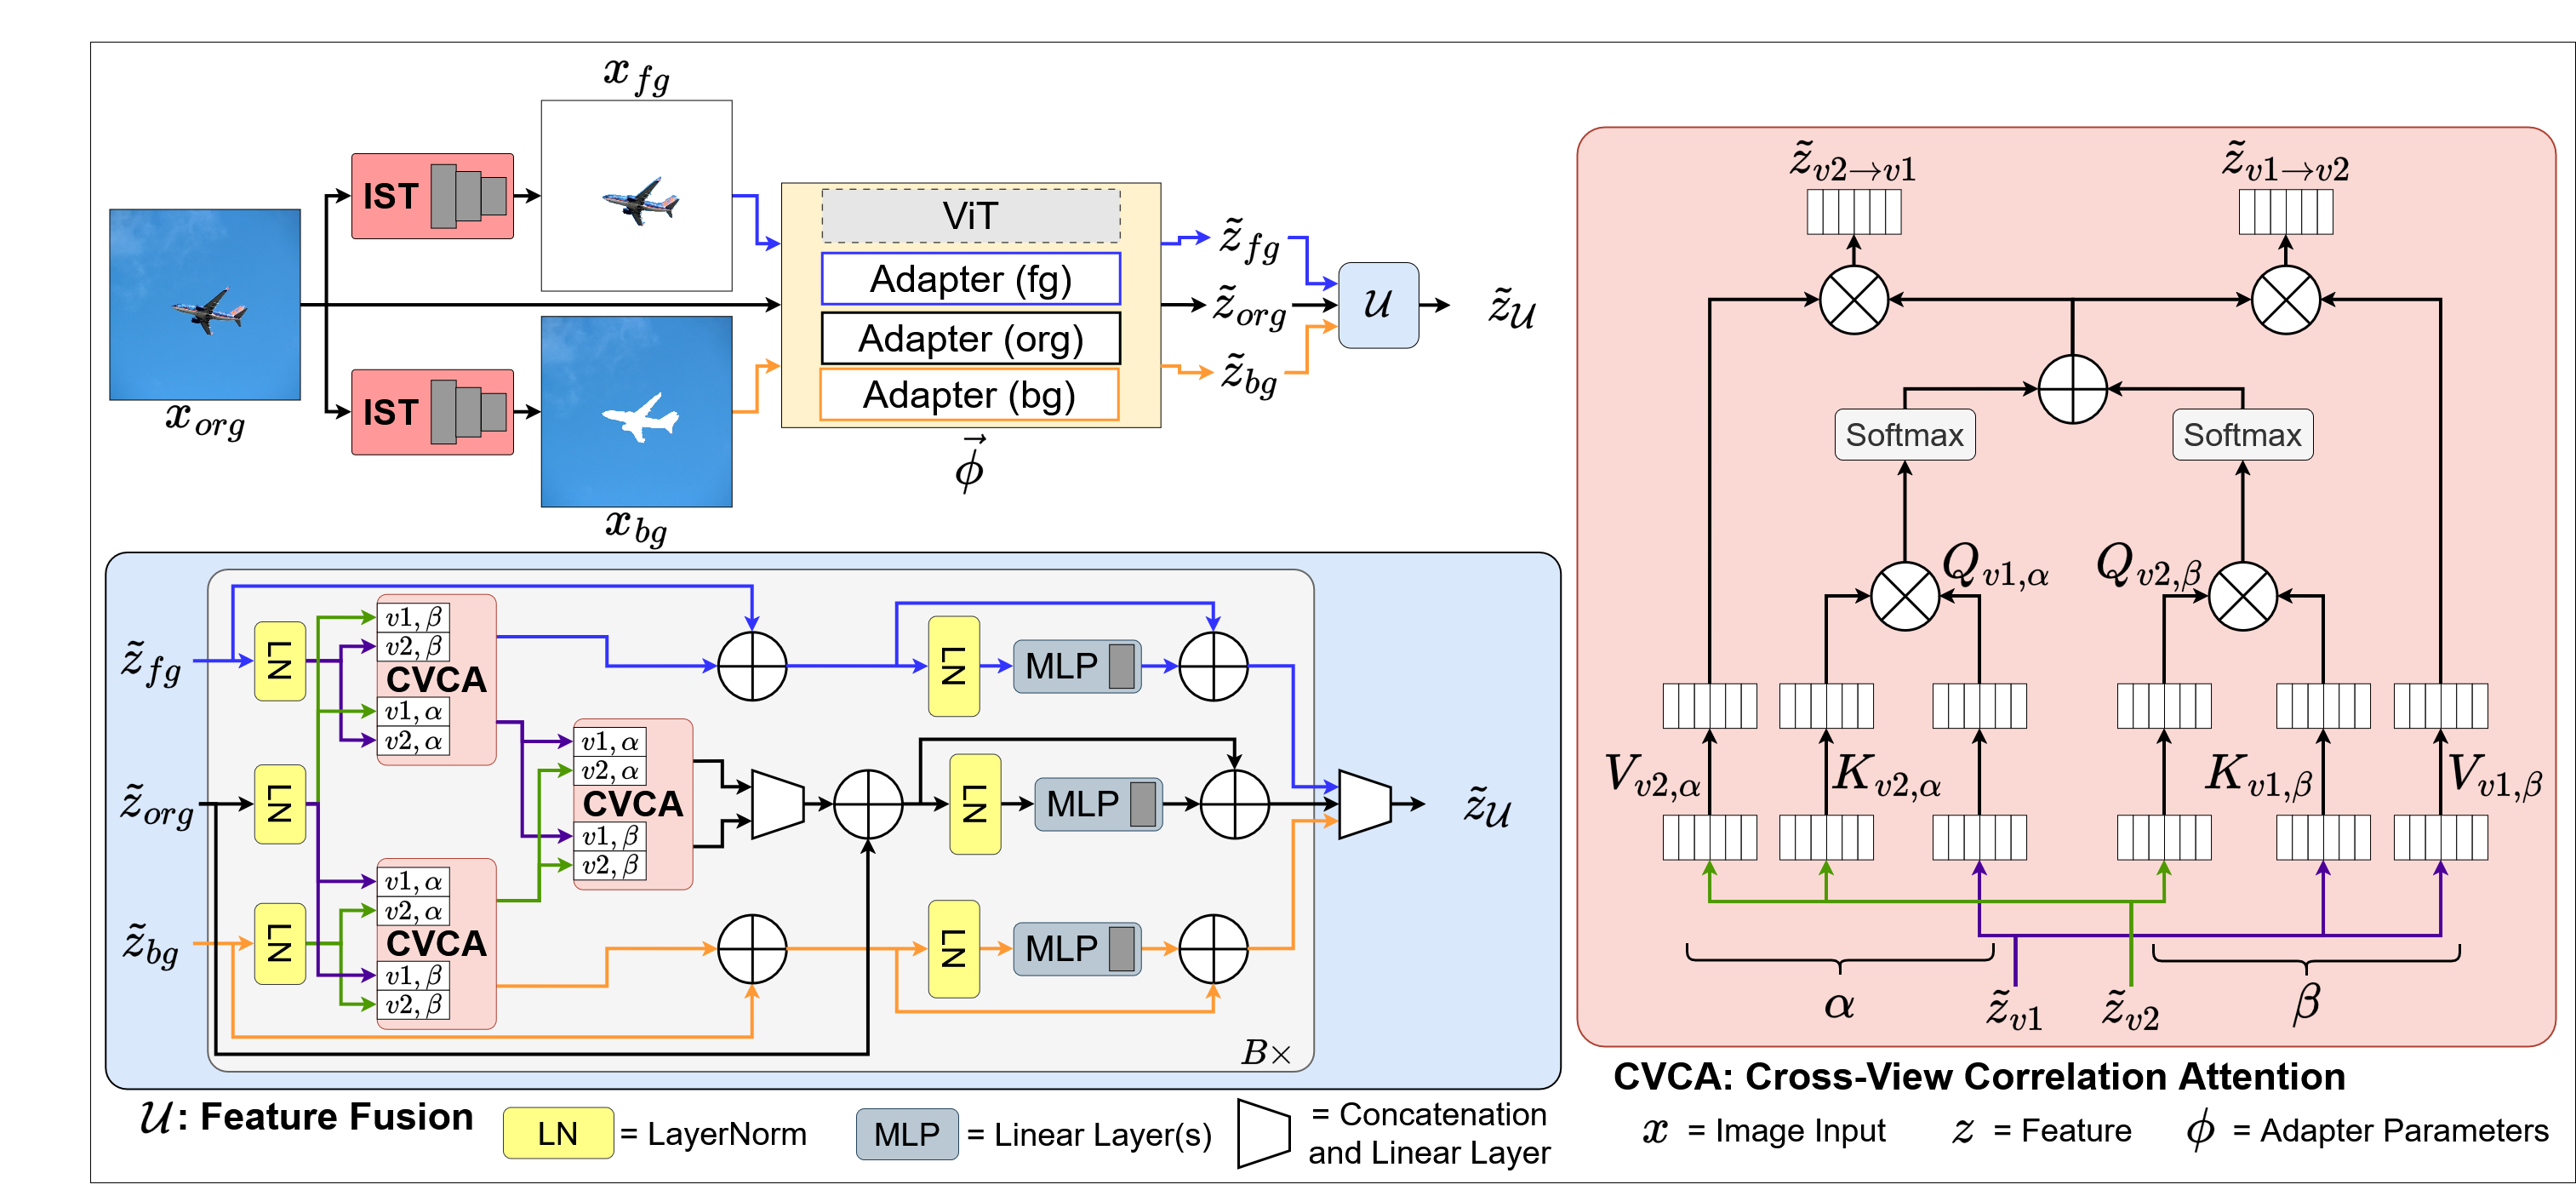
\includegraphics[width=1.\linewidth]{figures/casod_diagram}
	
	\caption{Model architecture of the proposed \sys. 
		%Black lines refer to the original or fused image features. Blue lines refer to foreground image features, orange lines refer to background image features. Best viewed in color. 
        $\alpha$ and $\beta$ are illustrative cues that connect views to CVCA modules.
	}
	\label{fig:casod_model_arch}
\end{figure*}

%Let $\mathcal{D}_{id} = \{(x_i, y_i)\}_{i=1}^N$ be the ID image classification dataset, where $y_i$ is the class label of image $x_i$, and $\mathcal{Y} = \{y_1, y_2, ... , y_R\}$ be the set of all ID class labels in $\mathcal{D}_{id}$. Our proposed method \sys builds an OOD detector (given \textit{only} $\mathcal{D}_{id}$) that detects whether an input image $x'$ is an ID or OOD sample. Figure \ref{fig:model_arch} shows the model architecture of \sys.  We segment each image $x$ in $\mathcal{D}_{id}$ into a foreground ($x_{fg}$) and a background ($x_{bg}$) view.  We still use the original image $x$ (from here notated as $x_{org}$ for clarity) as it contains integrated information. 
%The three views $x_{org}$, $x_{fg}$, $x_{bg}$ are fed to a view feature extractor, composed of a Vision Transformer-based \cite{dosovitskiy2020image} backbone equipped with \textit{view-specific} Adapters \cite{houlsby2019parameter} 
%to learn features $z_{org}$, $z_{fg}$, $z_{bg}$. In Sec.~\ref{sec:method-rep}, we discuss how the features are intelligently fused into a fused feature $z_{fused}$ via a unique \textit{cross-view correlation attention} fusion. Sec.~\ref{sec:method-train} describes how the whole system is trained end-to-end. Sec.~\ref{sec:method-ood} presents how the fused feature is used for OOD detection through distance-based scoring.
The \gls{sys} model architecture is shown in \ref{fig:casod_model_arch}. As previously detailed, the original image (\textit{org}) is segmented into the foreground (\textit{fg}) and background (\textit{bg}) views by the IST. The pre-trained VIT and Adapter set corresponding to each view is used to extract features $\tilde{Z}_{MV}$ while classification layers predict view-specific logits $\hat{Y}_{MV}$. The fusion component $\mathcal{U}$ in \gls{sys} utilizes a novel \textit{cross-view correlation attention} fusion mechanism to comprehensively extract and combine discriminative information from each view feature into a fused feature $\tilde{z}_{\mathcal{U}}$.

\subsection{Feature Learning}
\label{sec:casod_method-rep}

%Given the three views $x_{org}$, $x_{fg}$, $x_{bg}$ of image $x$, we employ a Vision Transformer (ViT) as a feature extractor. To \emph{increase parameter efficiency and mitigate computational costs}, we use a \textbf{frozen, pre-trained} ViT model and add three \textbf{trainable} LoRA Adapters \cite{hu2021lora} to each block, one per view. Each view $x_v$ (where $v \in \{org, fg, bg\}$) is fed to the ViT and its corresponding \textit{view-specific} Adapter at each block. The ViT and view-specific Adapter parameters for a view $v$ we denote as $\phi_{v}$ (with $\vec{\phi} = \{\phi_{org}, \phi_{fg}, \phi_{bg}\}$). The penultimate feature $z_v \in \mathbb{R}^{T \times d}$ is thus obtained via $z_v = \phi_v (x_v)$. Here, $T$ is the sequence length resulting from the patch embedding of the input image and prepending of class token $z_v^{0}$ and $d$ is the embedded feature dimension. Following the state-of-the-art ViT implementation, we add position encodings to the patches of the input images \cite{dosovitskiy2020image}. 
%Finally, the three view features $z_{org}$, $z_{fg}$, and $z_{bg}$ are fused using a cross-view correlation attention %\citep{vaswani2017attention} 
%%Transformer-inspired \citep{vaswani2017attention,dosovitskiy2020image} 
%fusion component (\textbf{FF} in Figure \ref{fig:model_arch}).
The three views of image $x$, $x_{org}$, $x_{fg}$, $x_{bg}$, are input to a \textbf{frozen, pre-trained} VIT model and three \textbf{trainable} LoRA Adapters \cite{hu2021lora} (one per view) at each block. The Adapters serve to \textit{mitigate computational costs by increasing parameter efficiency}, and myriad literature exists exploring the efficacy of Adapter-based tuning \cite{hanparameter}. In greater detail, each view $x_v$ (for $v \in \{org, fg, bg\}$) is passed through the VIT and corresponding \textit{view-specific} Adapter at each block in the VIT architecture (collectively denoted as $\phi_v$). Penultimate view-specific feature $\tilde{z}_v \in \mathbb{R}^{T \times d}$ is output from the feature extractor, $\tilde{z}_v = \phi_v (x_v)$. Following from the aforementioned Transformer procedure, $T$ is the sequence length from image patch embedding (including the prepended class token $\tilde{z}_{v}^{0}$) and $d$ is the dimension of embedded feature. Position encodings are also used with the image patches \cite{dosovitskiy2020image}. $\tilde{Z}_{MV} = \{\tilde{z}_{org}, \tilde{z}_{fg}, \tilde{z}_{bg}\}$ are fused using a fusion component $\mathcal{U}$ based on hierarchical aggregation of proposed cross-view correlation attention outputs.

%\textbf{Feature Fusion.} We use cross-view correlation attention (CVCA) modules (pink box in Figure \ref{fig:model_arch}) to learn \emph{cross-view} class-relevant discriminative features between (1) the original-foreground view pair, (2) the original-background view pair, and (3) the resulting cross-view feature pair. The feature fusion module receives as input $z_{org}$, $z_{fg}$, and $z_{bg}$ and is composed of a hierarchy of CVCA modules, three view-specific branches of linear connections, and a final combination operation.
\subsubsection{Feature Fusion}
Cross-view correlation attention (\gls{cvca}) (pink box in \ref{fig:casod_model_arch}, right side) learns \emph{cross-view} ID class-relevant discriminative features between
\begin{enumerate}
    \item the [org,fg] view pair,
    \item the [org,bg] view pair,
    \item the resulting cross-view feature pair.
\end{enumerate}
The fusion component $\mathcal{U}$ takes $\tilde{Z}_{MV}$ as input and passes it through a hierarchy of \gls{cvca} blocks, three view-specific linear connection branches, and a cumulative aggregation operation.

%Without loss of generality, we represent the inputs to a CVCA module as $z_{v1}$ and $z_{v2}$. A CVCA module takes $z_{v1}$ and $z_{v2}$ and extracts queries $Q_{v1} = FF_{Q,v1}(z_{v1}) \in \mathbb{R}^{T_{v1} \times d_{k}}$ from $z_{v1} \in \mathbb{R}^{T_{v1} \times d_{v1}}$ using feed-forward layer $FF_{Q,v1}$, and keys $K_{v2} = FF_{K,v2}(z_{v2}) \in \mathbb{R}^{T_{v2} \times d_{k}}$ and values $V_{v2} = FF_{V,v2}(z_{v2}) \in \mathbb{R}^{T_{v2} \times d_{w}}$ from $z_{v2}$ using feed-forward layers $FF_{K,v2}$ and $FF_{V,v2}$. Similarly, we can obtain $Q_{v2}$, $K_{v1}$, and $V_{v1}$ using feed-forward layers $FF_{Q,v2}$, $FF_{K,v1}$, and $FF_{V,v1}$. Note that in our implementation $T_{v1} = T_{v2}$ and $d_{k} = d_{w}$. These queries, keys, and values are then used to generate the cross-attention features $z_{v2 \rightarrow v1}$ and $z_{v1 \rightarrow v2}$
%\begin{equation}
%\begin{split}
%	U_{v2 \rightarrow v1} & = \text{softmax} \left( \frac{Q_{v1} K_{v2}^{\mathsf{T}}}{\sqrt{d_{k}}} \right) \\
%	U_{v1 \rightarrow v2} & = \text{softmax} \left( \frac{Q_{v2} K_{v1}^{\mathsf{T}}}{\sqrt{d_{k}}} \right) \\
%	A & = U_{v2 \rightarrow v1} + U_{v1 \rightarrow v2} \\
%	z_{v2 \rightarrow v1} & =  A V_{v2} \\
%	z_{v1 \rightarrow v2} & =  A V_{v1} \\
%	\{z_{v2 \rightarrow v1}, z_{v1 \rightarrow v2}\} & = CVCA(z_{v1}, z_{v2}),
%\end{split}
%\end{equation}
%where $A$ is the element-wise sum of the cross-view attention matrices $U_{v2 \rightarrow v1}$ and $U_{v1 \rightarrow v2}$, and (without loss of generality) $z_{v2 \rightarrow v1}$ is the product between the correlation cross-view attention matrix $A$ and the respective values $V_{v2}$.
\gls{cvca} operates on two views at a time, here denoted as $\tilde{z}_{v1}$ and $\tilde{z}_{v2}$ without loss of generality. $\tilde{z}_{v1} \in \mathbb{R}^{T_{v1} \times d_{v1}}$ is used to extract queries $Q_{v1} = FF_{Q,v1}(\tilde{z}_{v1}) \in \mathbb{R}^{T_{v1} \times d_{k}}$ using feed-forward layer $FF_{Q,v1}$. $\tilde{z}_{v2} \in \mathbb{R}^{T_{v2} \times d_{v2}}$ is used to extract 1) keys $K_{v2} = FF_{K,v2}(\tilde{z}_{v2}) \in \mathbb{R}^{T_{v2} \times d_{k}}$ using feed-forward layer $FF_{K,v2}$, and 2) values $V_{v2} = FF_{V,v2}(\tilde{z}_{v2}) \in \mathbb{R}^{T_{v2} \times d_{w}}$ using feed-forward layer $FF_{V,v2}$. $Q_{v2}$, $K_{v1}$, and $V_{v1}$ are obtained similarly using feed-forward layers $FF_{Q,v2}$, $FF_{K,v1}$, and $FF_{V,v1}$. Note that any feed-forward layer $FF$ is equivalent to a weight matrix $W$ and bias $b$ pair presented in previous sections for classification and other linear layer processing. In further specification, it is assumed that $T_{v1} = T_{v2}$ and $d_{k} = d_{w}$, a common assumption in literature and implementations \cite{dosovitskiy2020image}. Queries, keys, and values for $v1$ and $v2$ are used to computed cross-attention features $\tilde{z}_{v2 \rightarrow v1}$ and $\tilde{z}_{v1 \rightarrow v2}$
\begin{equation}
\begin{split}
	U_{v2 \rightarrow v1} & = \text{softmax} \left( \frac{Q_{v1} K_{v2}^{\mathsf{T}}}{\sqrt{d_{k}}} \right) \\
	U_{v1 \rightarrow v2} & = \text{softmax} \left( \frac{Q_{v2} K_{v1}^{\mathsf{T}}}{\sqrt{d_{k}}} \right) \\
	A & = U_{v2 \rightarrow v1} + U_{v1 \rightarrow v2} \\
	\tilde{z}_{v2 \rightarrow v1} & =  A V_{v2} \\
	\tilde{z}_{v1 \rightarrow v2} & =  A V_{v1} \\
	\{\tilde{z}_{v2 \rightarrow v1}, \tilde{z}_{v1 \rightarrow v2}\} & = CVCA(\tilde{z}_{v1}, \tilde{z}_{v2}).
\end{split}
\end{equation}
Importantly, $A$ is the element-wise sum of cross-view attention matrices $U_{v2 \rightarrow v1}$ and $U_{v1 \rightarrow v2}$ and embodies a critical advantage for \gls{cvca} over existing self-attention and cross-attention methods (see the Theoretical Analysis in Section \ref{sec:propwork-casod-theory}). Without loss of generality, the product between the \gls{cvca} matrix $A$ and respective value $V_{v2}$ results in $\tilde{z}_{v2 \rightarrow v1}$. 

%We use a hierarchy of CVCA modules to extract correlating features in the original and foreground views and original and background views ($LN$ is the LayerNorm operation)
%\begin{equation}
%\begin{split}
%	\{z_{fg \rightarrow org}, z_{org \rightarrow fg}\} & = CVCA(LN(z_{org}), LN(z_{fg}))  \\
%	\{z_{bg \rightarrow org}, z_{org \rightarrow bg}\} & = CVCA(LN(z_{org}), LN(z_{bg})).
%\end{split}
%\end{equation}
%The $org$-attended features $z_{fg \rightarrow org}$ and $z_{bg \rightarrow org}$ are further passed to a second-level CVCA module and concatenation layer to refine discriminatory features across all three views into a comprehensive $org$-view feature vector correlated across the $fg$ and $bg$ views $z_{fg,bg \rightarrow org}$,
%\begin{equation}
%\begin{split}
%	\{z_{org+fg}, z_{org+bg}\} & = CVCA(z_{fg \rightarrow org}, z_{bg \rightarrow org})
%	%\end{split}
%	%\end{equation}
%	%\begin{equation}
%	%\begin{split}
%	\\
%	z_{fg,bg \rightarrow org} & = f_{\psi_{fg,bg \rightarrow org}} ([z_{org+bg}; z_{org+fg}]),
%\end{split}
%\end{equation}
%where the $[\cdot\; ;\, \cdot]$ operator is concatenation in the embedded feature dimension $d$ of the feature vectors (from $\mathbb{R}^{T \times d}$ to $\mathbb{R}^{T \times 2d}$). The fully-connected layer $f_{\psi}$, parameterized by $\psi$, also operates on the $d$ dimension, reducing $z_{fg,bg \rightarrow org}$ from $\mathbb{R}^{T \times 2d}$ back to $\mathbb{R}^{T \times d}$.
\gls{sys} utilizes a hierarchy of \gls{cvca} blocks in $\mathcal{U}$, extracting correlating features in 1) the original and foreground views, and 2) the original and background views
\begin{equation}
\begin{split}
	\{\tilde{z}_{fg \rightarrow org}, \tilde{z}_{org \rightarrow fg}\} & = CVCA(LN(\tilde{z}_{org}), LN(\tilde{z}_{fg}))  \\
	\{\tilde{z}_{bg \rightarrow org}, \tilde{z}_{org \rightarrow bg}\} & = CVCA(LN(\tilde{z}_{org}), LN(\tilde{z}_{bg})).
\end{split}
\end{equation}
$LN$ is the LayerNorm operation \cite{xu2019understanding}. $\tilde{z}_{fg \rightarrow org}$ and $\tilde{z}_{bg \rightarrow org}$ are $org$-attended features, further passed to a second-level \gls{cvca} block and concatenation layer. These additional hierarchical operations further refine discriminative features from all three views into a comprehensive $org$-view feature $\tilde{z}_{fg,bg \rightarrow org}$ embodying information from correlated feature components in the $fg$ and $bg$ views
\begin{equation}
\begin{split}
	\{\tilde{z}_{org+fg}, \tilde{z}_{org+bg}\} & = CVCA(\tilde{z}_{fg \rightarrow org}, \tilde{z}_{bg \rightarrow org}) \\
	\tilde{z}_{fg,bg \rightarrow org} & = f_{\psi_{fg,bg \rightarrow org}} ([\tilde{z}_{org+bg}; \tilde{z}_{org+fg}]).
\end{split}
\end{equation}
Recall that $[\cdot\; ;\, \cdot]$ is the concatenation operator, in this case in the embedded feature dimension $d$ of feature (i.e. from $\mathbb{R}^{T \times d}$ to $\mathbb{R}^{T \times 2d}$). Fully-connected layer $f_{\psi}$ (parameterized by $\psi$) also operates on the $d$ dimension and reduces $\tilde{z}_{fg,bg \rightarrow org}$ from $\mathbb{R}^{T \times 2d}$ back to $\mathbb{R}^{T \times d}$.

%The resultant features from the CVCA modules are used with the initial view features to generate further view-informed features, summarized below
%\begin{equation}
%\begin{split}
%	\hat{S}_{org \rightarrow fg} & =  z_{org \rightarrow fg} + z_{fg} \\
%	\hat{S}_{org \rightarrow bg} & =  z_{org \rightarrow bg} + z_{bg} \\
%	\hat{S}_{fg,bg \rightarrow org} & =  z_{fg,bg \rightarrow org} + z_{org} \\
%	S_{org \rightarrow fg} & = f_{\psi_{org \rightarrow fg}} (LN(\hat{S}_{org \rightarrow fg})) + \hat{S}_{org \rightarrow fg} \\
%	S_{org \rightarrow bg} & = f_{\psi_{org \rightarrow bg}} (LN(\hat{S}_{org \rightarrow bg})) + \hat{S}_{org \rightarrow bg} \\
%	S_{fg,bg \rightarrow org} & = f_{\psi_{fg,bg \rightarrow org}} (LN(\hat{S}_{fg,bg \rightarrow org})) + \hat{S}_{fg,bg \rightarrow org}.
%\end{split}
%\end{equation}
%These operations, from input features $\{z_{org}, z_{fg}, z_{bg}\}$ to output features $\{S_{fg,bg \rightarrow org}, S_{org \rightarrow fg}, S_{org \rightarrow bg}\}$, can optionally be stacked on top of each other as a series of $B$ cross-view feature fusion blocks.
In \gls{sys}, features output from \gls{cvca} are used in combination with the initial, view-specific features to synthesize further view-informed features
\begin{equation}
\begin{split}
	\hat{S}_{org \rightarrow fg} & =  \tilde{z}_{org \rightarrow fg} + \tilde{z}_{fg} \\
	\hat{S}_{org \rightarrow bg} & =  \tilde{z}_{org \rightarrow bg} + \tilde{z}_{bg} \\
	\hat{S}_{fg,bg \rightarrow org} & =  \tilde{z}_{fg,bg \rightarrow org} + \tilde{z}_{org} \\
	S_{org \rightarrow fg} & = f_{\psi_{org \rightarrow fg}} (LN(\hat{S}_{org \rightarrow fg})) + \hat{S}_{org \rightarrow fg} \\
	S_{org \rightarrow bg} & = f_{\psi_{org \rightarrow bg}} (LN(\hat{S}_{org \rightarrow bg})) + \hat{S}_{org \rightarrow bg} \\
	S_{fg,bg \rightarrow org} & = f_{\psi_{fg,bg \rightarrow org}} (LN(\hat{S}_{fg,bg \rightarrow org})) + \hat{S}_{fg,bg \rightarrow org}.
\end{split}
\end{equation}
The collection of these computations, from inputs $\{\tilde{z}_{org}, \tilde{z}_{fg}, \tilde{z}_{bg}\}$ to outputs $\{S_{fg,bg \rightarrow org}, S_{org \rightarrow fg}, S_{org \rightarrow bg}\}$, can optionally be stacked sequentially as a series of $B$ cross-view feature fusion \emph{blocks}.

%The final fused feature is generated from the three view-informed features via a concatenation layer
%\begin{equation}
%z_{fused} = f_{\psi_{fused}} ([S_{fg,bg \rightarrow org}; S_{org \rightarrow fg}; S_{org \rightarrow bg}]).
%\end{equation}
The three view-informed features are fused into a comprehensive feature using a concatenation layer
\begin{equation}
\tilde{z}_{\mathcal{U}} = f_{\psi_{\mathcal{U}}} ([S_{fg,bg \rightarrow org}; S_{org \rightarrow fg}; S_{org \rightarrow bg}]).
\end{equation}

%\textbf{Fusion Features and Logits:} The class token of the fused feature $z_{fused}^{0}$ is used for OOD scoring (see Sec.~\ref{sec:method-ood}). View-specific feature $z_{org}^{0}$, $z_{fg}^{0}$, $z_{bg}^{0}$ are not directly used in detection because they are learned from limited information, degrading their OOD detection capability (see Sec.~\ref{sec:disc-ablation} for details). Classification heads for the fused and view-specific feature vectors are each implemented by a single linear layer. These classification layers produce fused prediction logits $\hat{y}_{fused}$ (given $z_{fused}^{0}$) and view-specific prediction logits $\hat{y}_{org}$, $\hat{y}_{fg}$, $\hat{y}_{bg}$ (given $z_{org}^{0}$, $z_{fg}^{0}$, and $z_{bg}^{0}$ respectively). 
\subsubsection{Fusion Features and Logits}
For OOD detection, the class token of the comprehensive feature $z_{\mathcal{U}} = \tilde{z}_{\mathcal{U}}^{0}$ is used. The view-specific features $\tilde{z}_{org}^{0}$, $\tilde{z}_{fg}^{0}$, $\tilde{z}_{bg}^{0}$ are not explicitly used for OOD detection (similar to \gls{sysa} and \gls{sysb}). An investigation into the limited OOD detection capabilities of view-specific features in comparison to fused features is conducted in Section \ref{sec:propwork-casod-disc}. For classification, linear layers parameterized by $W_{\mathcal{U}}$, $b_{\mathcal{U}}$ for the comprehensive feature and $W_v$, $b_v$ for each individual view are used to predict logits $\hat{y}_{\mathcal{U}}$ (given $z_{\mathcal{U}}$) and $\hat{y}_{org}$, $\hat{y}_{fg}$, $\hat{y}_{bg}$ (given $\tilde{z}_{org}^{0}$, $\tilde{z}_{fg}^{0}$, and $\tilde{z}_{bg}^{0}$ respectively).

\subsection{Model Training and Testing}
\label{sec:casod_method-train}

%We train \sys end-to-end using classification loss for each of the individual views as well as for the fused feature. The parameters $\phi_{v}$ ($ v \in \{org, fg, bg\}$) of each view feature extractor are learned using cross-entropy (CE) loss. Each view $v$ % $v \in \{org, fg, bg\}$ 
%has its view-specific CE loss $\mathcal{L}_{CE,v}$
%\begin{equation}
%\begin{aligned}
%    \mathcal{L}_{CE,v}(y, \hat{y}_v) & = -\sum_{c \in \mathcal{Y}} y_{c} \log(\hat{y}_{v,c}), \\
%\end{aligned}
%\end{equation}
%where $\hat{y}_{v,c}$ denotes the logit value of $\hat{y}_{v}$ for class $c$ and $y$ is the one-hot true label vector. We also define a fused feature CE loss $\mathcal{L}_{CE,fused}$ for the feature fusion head
%\begin{equation}
%\begin{aligned}
%    \mathcal{L}_{CE,fused}(y, \hat{y}_{fused}) & = -\sum_{c \in \mathcal{Y}} y_{c} \log(\hat{y}_{fused,c}), \\
%\end{aligned}
%\end{equation}
%where $\hat{y}_{fused,c}$ is the logit value of the final fused feature logit $\hat{y}_{fused}$ for class $c$. Note that fused feature information is additionally propagated to the individual view feature extractors to further tune them towards learning features optimal for fusion. The final loss $\mathcal{L}_{CE}$ is the combination of the fused feature and view-specific CE losses
%\begin{equation}
%\begin{aligned}
%    \mathcal{L}_{CE} ~= ~\smashoperator{\sum_{v \in \{fused, ~org, ~fg, ~bg\}}} \mathcal{L}_{CE,v} (y, \hat{y}_{v}).
%\end{aligned}
%\end{equation}
\gls{sys} is trained end-to-end using classification losses for each individual view and the comprehensive feature. Each view feature extractor $\phi_v$ ($v \in \{org, fg, bg\}$) is learned using a corresponding view specific cross-entropy (CE) loss  $\mathcal{L}_{CE,v}$
\begin{equation}
\begin{aligned}
    \mathcal{L}_{CE,v}(y, \hat{y}_v) & = -\sum_{c \in \mathcal{Y}} y_{c} \log(\hat{y}_{v,c}). \\
\end{aligned}
\end{equation}
$\hat{y}_{v,c}$ is the logit value of view $v$ predicted logits $\hat{y}_{v}$ for class $c$. $y$ is the one-hot true label vector. The comprehensive feature CE loss $\mathcal{L}_{CE,\mathcal{U}}$ is defined for predicted logits $\hat{y}_{\mathcal{U}}$
\begin{equation}
\begin{aligned}
    \mathcal{L}_{CE,\mathcal{U}}(y, \hat{y}_{\mathcal{U}}) & = -\sum_{c \in \mathcal{Y}} y_{c} \log(\hat{y}_{\mathcal{U},c}). \\
\end{aligned}
\end{equation}
Similar to above, $\hat{y}_{\mathcal{U},c}$ is the logit value of the fused comprehensive feature logit $\hat{y}_{\mathcal{U}}$ for class $c$. As $\hat{y}_{\mathcal{U}}$ takes view-specific features as input (via $\mathcal{U}$), fused feature information updates view-specific feature extractors through backpropagation of the $\mathcal{L}_{CE,\mathcal{U}}$ gradients. This further tunes the view-specific feature extractors towards learning features optimal for fusion. The final loss $\mathcal{L}_{CE}$ is the sum of comprehensive feature and view-specific CE losses
\begin{equation}
\begin{aligned}
    \mathcal{L}_{CE} ~= ~\smashoperator{\sum_{v \in \{\mathcal{U}, ~org, ~fg, ~bg\}}} \mathcal{L}_{CE,v} (y, \hat{y}_{v}).
\end{aligned}
\end{equation}
A contrastive loss term is not used in \gls{sys} due to the additional optimization complexity and relatively small performance increase (see Chapter \ref{diss_mvood_init} Section \ref{sec:propwork-scod-results}).

%\textbf{Testing:}
%As in training, the foreground and background views are first extracted from a test sample before the
%three views are fed to the system. This gives the fused feature vector $\tilde{z}_{fused}^{0}$ and fused logit $\hat{y}_{fused}$.
\subsubsection{Testing}
\gls{sys} follows the standard pipeline for testing. Specifically, foreground and background views are segmented from a test sample before the three views are provided to $\phi_{MV}$ and subsequently $\mathcal{U}$ as input. The result is the comprehensive feature vector $z_{\mathcal{U}}$ and logits $\hat{y}_{\mathcal{U}}$ per sample.

\subsection{OOD Detection}
\label{sec:casod_method-ood}

%\sys uses three views to learn a powerful fused feature. Thus, we use a state-of-the-art distance-based OOD detection technique, Mahalanobis distance (MD) \cite{lee2018simple,yang2022openood}, in conjunction with \sys for OOD detection as distance-based methods specialize in exploiting features for detecting OOD samples and their performance improves with feature richness. We note that, although only MD is discussed here, \sys is compatible with other OOD detection methods (results for these other methods are in Appendix Sec. D).
As in \gls{sysa} and \gls{sysb}, \gls{sys} learns a rich feature space from correlated view attention-based fusion. Thus it utilizes distance-based OOD detection methods to exploit this information domain for improved OOD detection \cite{lee2018simple,sun2022out,yang2022openood}. In this section, \gls{sys} with MD is presented as an illustration with a state-of-the-art distance-based method. However, as \gls{sys} outputs a feature vector and predicted logits, it is compatible with any post-hoc OOD detection method that uses either (or both) of these outputs. Results investigating \gls{sys} using other post-hoc OOD detection methods are detailed in Section \ref{sec:propwork-casod-disc}.

%MD measures the distance between a sample and a Gaussian distribution. Empirical class means $\hat{\mu}_{c}$ and covariance matrices $\hat{\Sigma}$ are computed from the training dataset $\mathcal{D}_{id}$ using the final fused feature $z_{fused}^{0}$
%\begin{equation}
%\begin{aligned}
%\hat{\mu}_{c} & = \frac{1}{N_{c}} \sum_{i:y_{i}=c} z_{fused,i}^{0} \\
%\hat{\Sigma} & = \frac{1}{N} \sum_{c} \sum_{i:y_{i}=c} (z_{fused,i}^{0} - \hat{\mu}_{c}) (z_{fused,i}^{0} - \hat{\mu}_{c})^\top, \\
%\end{aligned}
%\end{equation}
%where $N_{c}$ is the number of samples with class $c$.  Given a test instance $x'$, \sys first extracts feature $z_{fused}^{0'}$ and then computes the distance between it and the nearest class-conditional Gaussian distribution for the view, which is the final OOD score for the view 
%\begin{equation}
%\scalebox{0.93}{$
%M_{MD}(x') = \max_{c} (-(z_{fused}^{0'} - \hat{\mu}_{c})^\top \hat{\Sigma}_{v}^{-1} (z_{fused}^{0'} - \hat{\mu}_{c})). \\
%$}
%\end{equation}
%For OOD distance scores (i.e. $M_{MD}$), $x'$ with higher (lower) scores are closer to ID (OOD) samples \cite{sun2022out}. 
MD in \gls{sys} uses the comprehensive feature vector $z_{\mathcal{U}}$ to estimate the empirical class means $\hat{\mu}_{c}$ (for all $c \in C$) and covariance matrix $\hat{\Sigma}$
\begin{equation}
\begin{aligned}
\hat{\mu}_{c} & = \frac{1}{N_{c}} \sum_{i:y_{i}=c} z_{\mathcal{U},i} \\
\hat{\Sigma} & = \frac{1}{N} \sum_{c} \sum_{i:y_{i}=c} (z_{\mathcal{U},i} - \hat{\mu}_{c}) (z_{\mathcal{U},i} - \hat{\mu}_{c})^\top, \\
\end{aligned}
\end{equation}
with $N_c$ as the number of samples in class $c$. OOD detection is performed with a test sample $x'$ by first using \gls{sys} to extract $z_{\mathcal{U}}'$. The distance between $z_{\mathcal{U}}'$ and the nearest class-conditional Gaussian distribution is the final OOD score
\begin{equation}
\scalebox{0.93}{$
M_{MD}(x') = \max_{c} (-(z_{\mathcal{U}}' - \hat{\mu}_{c})^\top \hat{\Sigma}_{v}^{-1} (z_{\mathcal{U}}' - \hat{\mu}_{c})). \\
$}
\end{equation}
%The implementation of MD for \sysb is very similar to that in \sysa. However, given that \sysb uses a combination of view-specific features, cross-view features, and a comprehensive fused feature, multiple empirical class means and covariance matrices must be defined. \sysb calculates empirical class means $\hat{\mu}_{c,v}$ and covariance matrices $\hat{\Sigma}_{v}$ for each view feature $v \in \{org, fg, bg, org+fg, org+bg, fg+bg, fused\}$. A test sample $x'$ is processed by \sysb into feature vector $z'_{v}$. Distances are computed between $z'_{v}$ and the nearest class-conditional Gaussian distribution for view $v$. The negative distance is the OOD score for view $v$
%\begin{equation}
%\begin{aligned}
%    S_{MD,v}(x') = \max_{c} (-(z_{v}' - \hat{\mu}_{c,v})^\top \hat{\Sigma}_{v}^{-1} (z_{v}' - \hat{\mu}_{c,v})). \\
%\end{aligned}
%\end{equation}

%\sys uses three views to learn a powerful fused feature and fused logit. Thus, we use a state-of-the-art OOD detection technique, Virtual-logit Matching (ViM) \cite{wang2022vim}, in conjunction with \sys for OOD detection as it specializes in exploiting class-agnostic information in features and class-dependent information in logits. With features that contain more ID discriminative features, the performance of ViM increases. Note that, although only ViM is discussed here, \sys is compatible with other OoD detection methods (results for these other methods are in Appendix Sec. XXX).
%
%ViM converts the feature $z^{0}_{fused}$ for sample $x'$ into a virtual logit used for OOD scoring. The virtual logit is calculated by defining a bias-free principal subspace $P$ using the training dataset features $\mathbf{Z}$ shifted to origin $\mathbf{o} = -(\mathbf{W}^{T})^{+}\mathbf{b}$ with $\mathbf{W}$ and $\mathbf{b}$ as the classification head weight and bias respectively. The eigendecomposition on the matrix $\mathbf{Z}^{T}\mathbf{Z} = \mathbf{Q} \mathbf{\Lambda} \mathbf{Q}^{-1}$ results in eigenvalues $\mathbf{\Lambda}$ sorted decreasingly and the matrix $\mathbf{Q}$. The ($D$+1)-th column to the last column of $\mathbf{Q}$ give the new matrix $\mathbf{R} \in \mathbb{R}^{p \times (p-D)}$ for some value $D$. In our experiments, $p = 768$ and we use $D = 512$. The virtual logit $\hat{y}_{0}$ is the norm of the residual rescaled by a constant $\alpha$
%\begin{equation}
%    \hat{y}_{0} = \alpha || z^{P^{\perp}} || = \alpha \sqrt{z^{T} \mathbf{R} \mathbf{R^{T}} z}
%\end{equation}
%The rescaling factor $\alpha$ is calculated from the training dataset predicted logits $\hat{y}$
%\begin{equation}
%    \alpha = \frac{\sum_{i=1}^{N} \max_{j=1,\dots,C} {\hat{y}_{j}^{i}}}{\sum_{i=1}^{N} || z_{i}^{P^{\perp}} ||}
%\end{equation}
%Finally, the virtual logit is appended to the model predicted logits and the softmax is computed. The resulting probability associated with the virtual logit is the OoD score $M_{ViM}$
%\begin{equation}
%    M_{ViM}(x) = \frac{e^{\alpha \sqrt{z^{T} \mathbf{R} \mathbf{R^{T}} z}}}{\sum_{i=1}^{C} e^{\hat{y}_{i}} + e^{\alpha \sqrt{z^{T} \mathbf{R} \mathbf{R^{T}} z}}}
%\end{equation}
%For OOD scores (i.e. $M_{ViM}$), $x'$ with higher (lower) scores are closer to ID (OOD) samples \cite{sun2022out}.


\section{Theoretical Analysis}
\label{sec:propwork-casod-theory}

\subsection{Qualitative Justification}

%{\color{blue}To mathematically support this in \sys, note that the SA attention matrix is computed from the concatenated view features $A_{SA} \in \mathbb{R}^{3T \times 3T}$, while the CVCA attention matrices are computed from two view features $A_{CVCA,v1 \rightarrow v2} \in \mathbb{R}^{T \times T}$. This implies that the denominator of the softmax in $A_{SA}$ is greater than the denominator of the softmax in each $A_{CVCA,v1 \rightarrow v2}$, $\sum_{j=1}^{3T} e^{a_{SA,j}} > \sum_{j=1}^{T} e^{a_{CVCA,j}}$ where $a$ is the pre-softmax attention value. Furthermore, CVCA is the sum of both view attention matrices $A_{CVCA} = A_{CVCA,v1 \rightarrow v2} + A_{CVCA,v2 \rightarrow v1}$. Following from these, SA \textbf{reduces} the magnitude of both patch activations while CVCA \textbf{additively reinforces} them. See Appendix Sec. E.2 for further analysis details.} %\sys performs significantly better. %While MaxPooling is sometimes superior for simpler far-OOD datasets, the feature details learned via bidirectional cross-view attention are crucial for near-OOD datasets. %Max-pooling is unable to learn these discriminative features and is weak at detecting near-OOD samples.
%{\color{purple}
The performance of CASOD fundamentally depends on the CVCA operation in the proposed fusion architecture. The significance of this operation is demonstrated via a comparison between CVCA attention computations and the standard self-attention (SA) computations in Transformer models \cite{vaswani2017attention} and throughout modern deep learning literature \cite{vaswani2017attention,dosovitskiy2020image,khan2023survey}. The theoretical analysis presented in this section begins with a high-level qualitative justification which can be read as a mathematical introduction to the theory to follow. To assist, please refer to \ref{fig:casod_model_arch} for an illustration of the CVCA architecture. The multi-view SA architecture considered here uses a concatenated view feature as input to an SA block (see \ref{fig:bkgd-attn_example} for an illustration). Thus, the comparison is between CVCA and SA as a fusion mechanism for discriminative feature learning and subsequent OOD detection. The motivating question is if CVCA offers improvements over SA.

\begin{figure*}
	\centering
	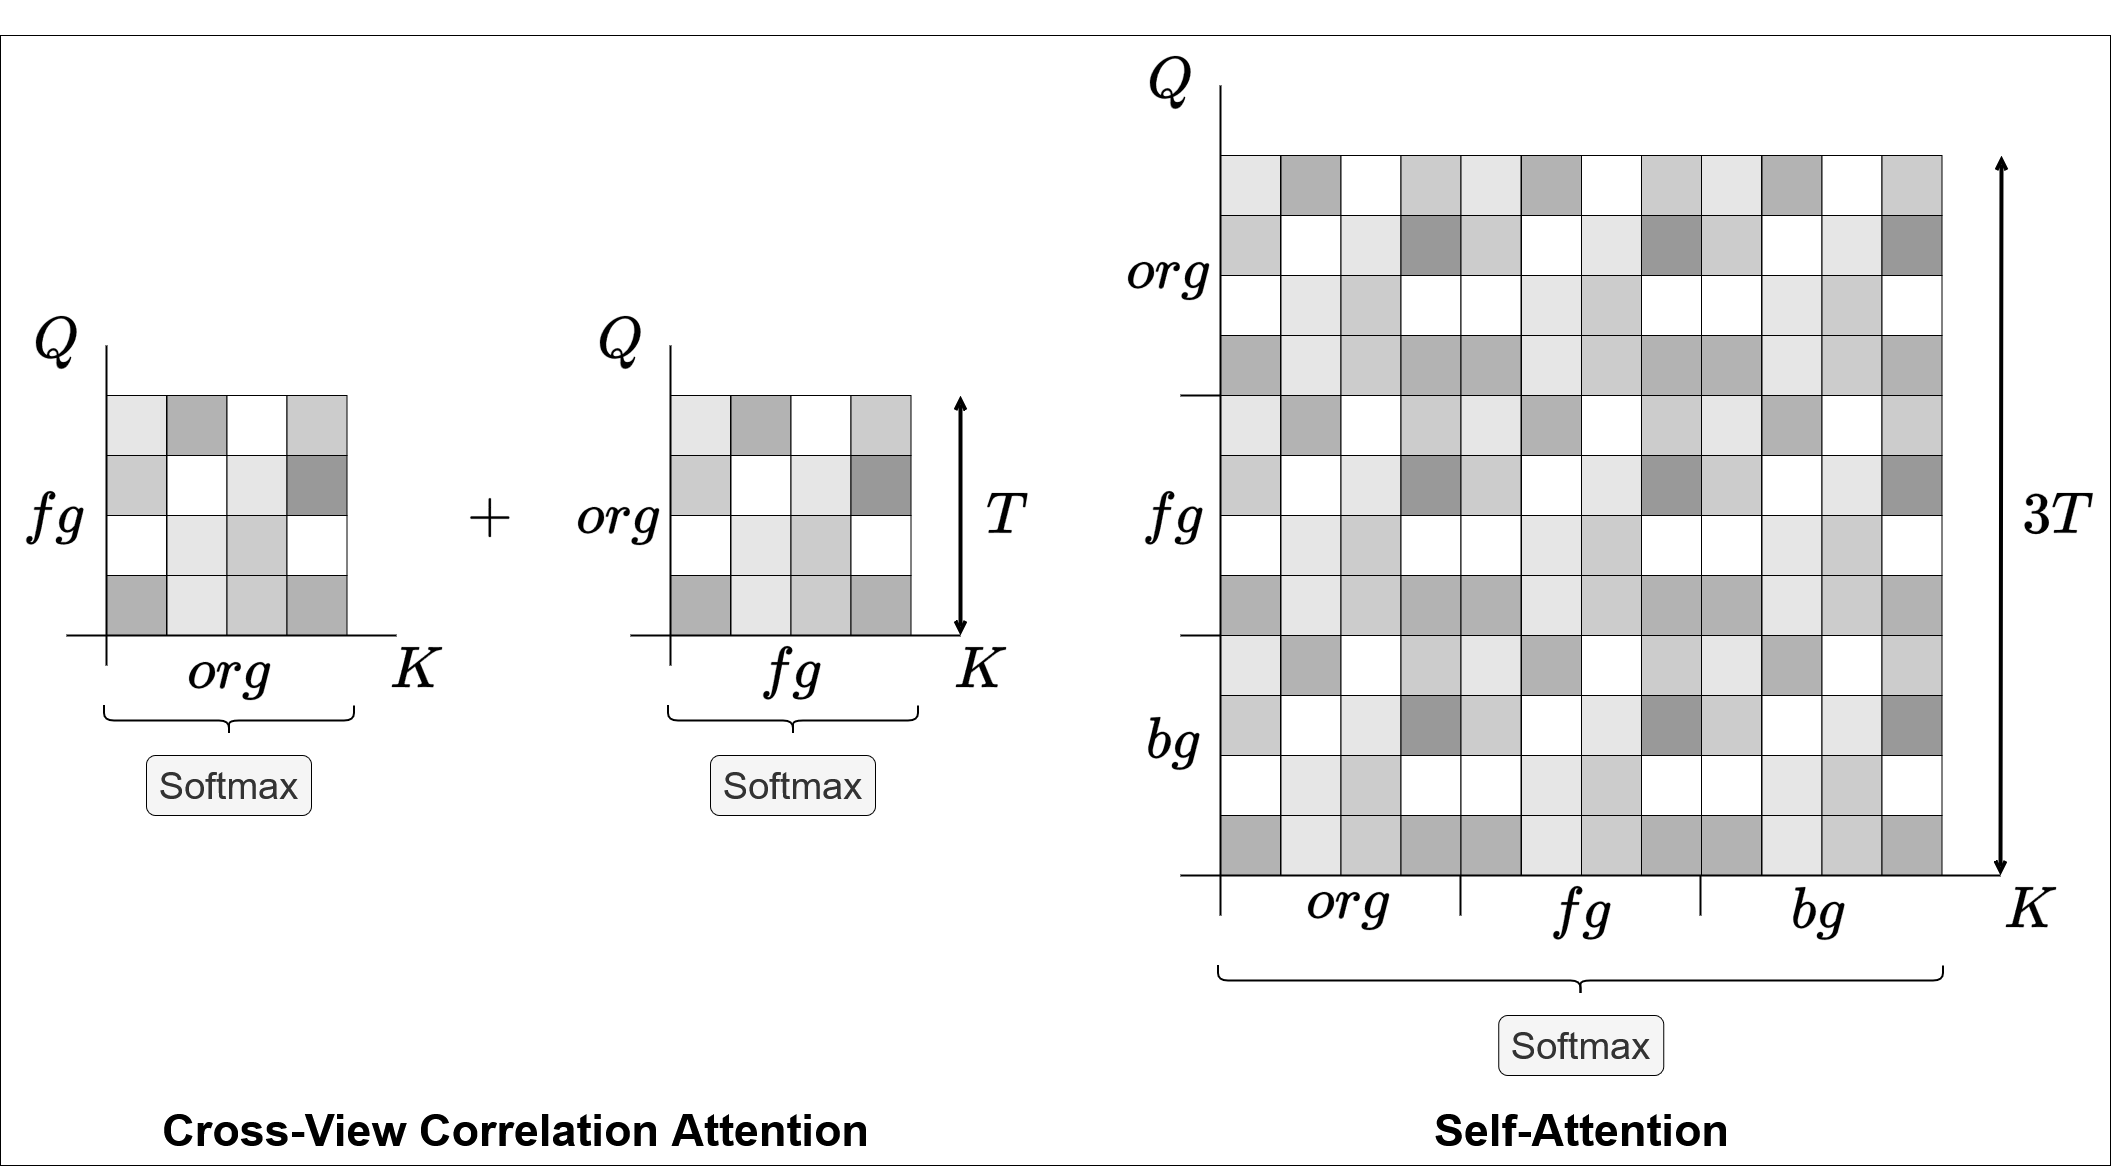
\includegraphics[width=1.\linewidth]{figures/matrix_attention_describe}
	\caption{The attention matrices in CVCA and SA are completely different, with CVCA allowing for \textbf{higher attention values} across features. The addition of cross-view attention matrices and smaller token dimensions in CVCA ensure greater emphasis of view features.
	}
	\label{fig:theory_matrix_ref}
\end{figure*}

SA attention matrices $A_{SA} \in \mathbb{R}^{3T \times 3T}$ are computed from the \emph{concatenated} view features (see \ref{fig:theory_matrix_ref}). CVCA attention matrices $A_{CVCA,v1 \rightarrow v2} \in \mathbb{R}^{T \times T}$ are computed from two view features (see \ref{fig:theory_matrix_ref}). Given identical input features $\tilde{z}$ and weight matrices $W_Q, W_K$, the higher dimensionality of SA attention matrices guarantees that the denominator of the softmax in $A_{SA}$ is greater than the denominator of the softmax in each $A_{CVCA,v1 \rightarrow v2}$, i.e. $\sum_{j=1}^{3T} e^{a_{SA,j}} > \sum_{j=1}^{T} e^{a_{CVCA,j}}$ where $a$ is the pre-softmax attention value. Furthermore, CVCA is the sum of both view attention matrices $A_{CVCA} = A_{CVCA,v1 \rightarrow v2} + A_{CVCA,v2 \rightarrow v1}$. In this setting, SA \textbf{reduces} the magnitude of patch activations while CVCA \textbf{additively reinforces} them.

However, in practice, it is not guaranteed that the input features $\tilde{z}$ nor the weight matrices $W_Q, W_K$ are the same in both SA and CVCA architectures. A more principled analysis is beneficial in isolating the conditions for CVCA to improve upon SA.
%}

%\subsection{Assumptions and Prerequisites}
%
%{\color{purple}
%
%}

%\subsection{Guarantees}
\subsection{Theoretical Findings}

%{\color{blue}
%(\textbf{NEW ATTEMPT} %general direction idea: if we can show org, fg, bg features are approximately the same under each paradigm, then this is guaranteed)
%Consider a particular high-activation patch in the CVCA attention matrix $p^* \in A_{CVCA,i}$ at index $j$. Assume the patch is exclusively from only one of the view attention matrices $p^* = \text{softmax}(z_{v1} W_{Q,v1} W_{K,v2}^{\intercal} z_{v2}^{\intercal})_{i,j} + 0$. We also distinguish the patch probabilities $p$ and the patch values before softmax as $a$.
%
%We analyze the conditions for self-attention to similarly identify and emphasize this critical high-attention patch. That is, $p^*_{SA} \geq p^*_{CVCA}$. We rewrite this expression as follows:
%\begin{equation}
%    \frac{e^{a^*_{SA}}}{\sum_{3T} e^{a_{SA}}} \geq \frac{e^{a^*_{CVCA}}}{\sum_{T} e^{a_{CVCA}}}
%\end{equation}
%\begin{equation}
%    e^{a^*_{SA}} \geq e^{a^*_{CVCA}} \frac{\sum_{3T} e^{a_{SA}}}{\sum_{T} e^{a_{CVCA}}}
%\end{equation}
%\begin{equation}
%    a^*_{SA} \geq a^*_{CVCA} + \ln{(\sum_{3T} e^{a_{SA}})} - \ln{(\sum_{T} e^{a_{CVCA}})}
%\end{equation}
%\begin{align}
%    a^*_{SA} \geq\ & a^*_{CVCA} + \ln{(e^{a^*_{SA}})} + \ln{(1 + \sum_{3T-1} \frac{e^{a_{SA}}}{e^{a^*_{SA}}})} \\
%    & - \ln{(e^{a^*_{CVCA}})} - \ln{(1 + \sum_{T-1} \frac{e^{a_{CVCA}}}{e^{a^*_{CVCA}}})}
%\end{align}
%\begin{equation}
%    1 + \sum_{T-1} \frac{e^{a_{CVCA}}}{e^{a^*_{CVCA}}} \geq 1 + \sum_{3T-1} \frac{e^{a_{SA}}}{e^{a^*_{SA}}}
%\end{equation}
%\begin{equation}
%    \frac{\sum_{T-1} e^{a_{CVCA}}}{\sum_{3T-1} e^{a_{SA}}} \geq e^{a^*_{CVCA} - a^*_{SA}}
%\end{equation}
%
%We show that this condition is not satisfied in the general case with high probability. We make two assumptions following from existing theoretical work:
%\begin{itemize}
%    \item \textbf{Assumption 1} The intermediate features $z$ in both SA and CVCA are bounded [A1].
%    \item \textbf{Assumption 2} The weight matrices $W_Q$, $W_K$, and $W_V$ in both SA and CVCA are bounded [A2,A3].
%\end{itemize}
%
%% from before:
%% https://proceedings.mlr.press/v119/xiong20b/xiong20b.pdf
%% https://arxiv.org/pdf/2305.03210
%% new potential:
%% https://arxiv.org/pdf/1511.07543 (not guaranteed same)
%% https://dl.acm.org/doi/pdf/10.1145/3728458 (not guaranteed same)
%% 
%
%%Assumption 1 is given through the concentration properties of LayerNorm operations. Assumption 2 is fundamental to efficient attention computation in practice. These assumptions immediately give that the patch values $a_{SA}$ and $a_{CVCA}$ are also bounded. {\color{red}TODO: what to do from here? are any of these options feasible?
%%\begin{enumerate}
%%    \item claim that $a^*_{CVCA} \approx a^*_{SA}$ from optimizing the same objective, then try and show the left-hand side denominator will almost always be larger than the numerator
%%    \item claim that $z$ are similar in SA and CVCA due to optimization of the same objective, claim that all Q, K project to similar attention matrices for SA and CVCA due to optimization of the same objective
%%    \item 
%%\end{enumerate}
%%}
%}
%{\color{purple}

\subsubsection{Preliminary Information}
Self-attention (SA) and cross-attention (CA) are reiterated here (see Chapter \ref{diss_bkgd} for further details). Note that notations here generally follow those presented in Chapter \ref{diss_bkgd} for Attention mechanisms but more specifically follow those in the previous section for CVCA (Section \ref{sec:propwork-casod-method}). The exception is that inputs (i.e. features) for the rest of this section are represented as $x$ instead of $\tilde{z}$ for generality. In SA,
an input $x$ is projected into matrices $Q$, $K$, and $V$ using respective parameters $W_Q \in \mathbb{R}^{d \times d_k}$, $W_K \in \mathbb{R}^{d \times d_k}$, $W_V \in \mathbb{R}^{d \times d_v}$
\begin{equation}
\begin{aligned}
    Q & = x W_Q \\
    K & = x W_K \\
    V & = x W_V. \\
\end{aligned}
\end{equation}
The attention $A$ is calculated from $Q$, $K$, and $V$, intermediary attention values $\alpha$, and the softmax function
\begin{equation}
\begin{aligned}
    \alpha(Q,K,d_k) & = \text{softmax} (\frac{Q K^{\mathsf{T}}}{\sqrt{d_k}}) \\
    A(\alpha,V) & = \alpha V.
\end{aligned}
\end{equation}
The softmax function is defined as follows
\begin{equation}
\begin{aligned}
    o(x)_i = \frac{e^{x_i}}{\sum_{j=1}^{K} e^{x_j}}, \\
\end{aligned}
\end{equation}
for some vector $x \in \mathbb{R}^K$ and resulting in vector $o(x) \in (0,1)^K$. Intermediary attention values $\alpha$ and attention values $A$ can be further delineated by patch. That is, for patch indices $i,j$
\begin{equation}
\begin{aligned}
    \alpha_{ij} & = \text{softmax} (\frac{Q_i K_j^{\mathsf{T}}}{\sqrt{d_k}}), \\
\end{aligned}
\end{equation}
and similar for any $A_{ij}$.
CA takes as input two inputs $x_1$ and $x_2$. $Q$, $K$, and $V$ are computed
\begin{equation}
\begin{aligned}
    Q & = x_1 W_Q \\
    K & = x_2 W_K \\
    V & = x_2 W_V, \\
\end{aligned}
\end{equation}
before attention is calculated. Note that parameters in CA are labeled according to their respective origin input, e.g. $Q_1$, $K_2$
\begin{equation}
\begin{aligned}
    \alpha(Q_1,K_2,d_k) & = \text{softmax} (\frac{Q_1 K_2^{\mathsf{T}}}{\sqrt{d_k}}) \\
    A(\alpha,V_2) & = \alpha V_2.
\end{aligned}
\end{equation}

Cross-view correlation attention (CVCA), proposed in the previous section (see Section \ref{sec:propwork-casod-method}), is inspired by CA and considers inputs from two views $x_{v1}, x_{v2}$. Attention is computed using view-associated preliminary attention values $\alpha_{12}, \alpha_{21}$ as follows
\begin{equation}
\begin{aligned}
    Q_{1,v1} & = x_{v1} W_{Q,1} \\
    K_{1,v2} & = x_{v2} W_{K,1} \\
    Q_{2,v2} & = x_{v2} W_{Q,2} \\
    Q_{2,v1} & = x_{v1} W_{K,2} \\
    \alpha_{12} & = \text{softmax} (\frac{Q_{1,v1} K_{1,v2}^{\mathsf{T}}}{\sqrt{d_{k_{v1}}}}) \\
    \alpha_{21} & = \text{softmax} (\frac{Q_{2,v2} K_{2,v1}^{\mathsf{T}}}{\sqrt{d_{k_{v2}}}}) \\
    \alpha & = \alpha_{12} + \alpha_{21}. \\
\end{aligned}
\end{equation}
Each preliminary attention value is computed with a corresponding $Q,K$, with $\alpha_{12}$ using $Q_1,K_1$ and $\alpha_{21}$ using $Q_2,K_2$.
%Any preliminary attention value $\alpha$ can be further delineated as the raw attention values $a$ prior to application of the softmax function, that is
%\begin{equation}
%\begin{aligned}
%    a_{ij} & = (\frac{Q_i K_j^{\mathsf{T}}}{\sqrt{d_k}}) \\
%    \alpha_{ij} & = \text{softmax} (a_{ij}). \\
%\end{aligned}
%\end{equation}
Henceforth in this section, the preliminary attention values $\alpha$ are referred to equivalently as the ``attention values'' or generally as ``attention'' in SA and CVCA.

For SA, the input $x$ in multi-view systems is a combination of all views, that is the original view $x_{org}$, the foreground view $x_{fg}$, and the background view $x_{bg}$. Specifically, $x$ in SA is a concatenation of all three view features
\begin{equation}
\begin{aligned}
    x = [x_{org} ; x_{fg} ; x_{bg}], \\
\end{aligned}
\end{equation}
with $x \in \mathbb{R}^{3T \times d}$, as each view feature $x_v \in \mathbb{R}^{T \times d}$ for $v \in \{org, fg, bg\}$. Each input for CVCA is exactly one of $x_{org}, x_{fg}, x_{bg}$.

\subsubsection{Main Findings}
Consider a discriminative high-activation patch $\alpha^*_{CVCA}$ in a CVCA attention matrix $\alpha^*_{CVCA} = \alpha_{CVCA,i^*j^*}$ for row $i^*$ at index $j^*$. Here, only one of the preliminary attention matrices is considered for comparison, i.e. only $\alpha_{12}$. The relationship between SA and CVCA for this discriminative high-activation patch can be expressed as
\begin{equation}
\begin{aligned}
    \alpha^*_{SA} \? \alpha^*_{CVCA}, \\
\end{aligned}
\label{peqn:1}
\end{equation}
where the $\?$ operator delineates an unknown relationship between the two operands. The goal is to identify the relationship between the two attention values and replacing the $\?$ operator with an informative, formal inequality. In CVCA, $\alpha_{12}$ must include $x_{org}$ as one of the inputs ($x_1$ for the rest of the analysis) and $x_2 = x_{fg}$ is considered as the other input without loss of generality. The expansion of \ref{peqn:1} follows by taking the softmax of both sides
\begin{equation}
\begin{aligned}
    %\alpha^*_{SA}  \alpha^*{CVCA}. \\
    \frac{e^{\alpha^*_{SA}}}{\sum_{k=1}^{3T} e^{\alpha_{SA,k}}} \? \frac{e^{\alpha^*_{CVCA}}}{\sum_{k=1}^{T} e^{\alpha_{CVCA,k}}}. \\
\end{aligned}
\label{peqn:2}
\end{equation}
The expression \ref{peqn:2} can be rearranged as such
\begin{align}
    %\alpha^*_{SA}  \alpha^*{CVCA}. \\
    e^{\alpha^*_{SA}} & \? e^{\alpha^*_{CVCA}} \frac{\sum_{k=1}^{3T} e^{\alpha_{SA,k}}}{\sum_{k=1}^{T} e^{\alpha_{CVCA,k}}} \nonumber \\
    \alpha^*_{SA} & \? \ln (e^{\alpha^*_{CVCA}}) + \ln (\sum_{k=1}^{3T} e^{\alpha_{SA,k}}) - \ln (\sum_{k=1}^{T} e^{\alpha_{CVCA,k}}) \nonumber \\
    \alpha^*_{SA} & \? \alpha^*_{CVCA} + \ln (e^{\alpha^*_{SA}}) + \ln (1 + \sum_{k=1}^{3T-1} \frac{e^{\alpha_{SA,k}}}{e^{\alpha^*_{SA}}}) - \ln (e^{\alpha^*_{CVCA}}) - \ln (1 + \sum_{k=1}^{T-1} \frac{e^{\alpha_{CVCA,k}}}{e^{\alpha^*_{CVCA}}}). \label{peqn:3}
\end{align}
The isolation of the $\alpha^*_{SA}, \alpha^*_{CVCA}$ terms from the summations follows from the analysis of the summation, here shown for the SA term but identically applicable to the CVCA term
\begin{equation}
\begin{aligned}
    \ln (\sum_{k=1}^{3T} e^{\alpha_{SA,k}}) & = e^{\alpha^*_{SA}} + e^{\alpha_{SA,1}} + e^{\alpha_{SA,2}} + \dots \\
    & = \ln (e^{\alpha^*_{SA}} (1 + \frac{e^{\alpha_{SA,1}}}{e^{\alpha^*_{SA}}} + \frac{e^{\alpha_{SA,2}}}{e^{\alpha^*_{SA}}} + \dots)) \\
    & = \ln (e^{\alpha^*_{SA}}) + \ln (1 + \sum_{k=1}^{3T-1} \frac{e^{\alpha_{SA,k}}}{e^{\alpha^*_{SA}}}). \\
\end{aligned}
\end{equation}
It is assumed that the discriminative high-activation patches $\alpha^*$ represent discriminative features learned by the model and are thus nearly identical in both SA and CVCA.
\begin{assumption}
    $\alpha^*_{SA} = \alpha^*_{CVCA} + E^*,$ \\
    $\cancelto{\simeq 0}{E^*}$ \\
    %$\cancelto{\approx 0}{A}$
    for some error $E^*$.
\label{pass:1}
\end{assumption}
%\begin{align}
%    %\alpha^*_{SA}  \alpha^*{CVCA}. \\
%    e^{\alpha^*_{SA}} & \? e^{\alpha^*_{CVCA}} \frac{\sum_{k=1}^{3T} e^{\alpha_{SA,k}}}{\sum_{k=1}^{T} e^{\alpha_{CVCA,k}}} \\
%    \alpha^*_{SA} & \? \ln (e^{\alpha^*_{CVCA}}) + \ln (\sum_{k=1}^{3T} e^{\alpha_{SA,k}}) - \ln (\sum_{k=1}^{T} e^{\alpha_{CVCA,k}}) \\
%    \alpha^*_{SA} & \? \alpha^*_{CVCA} + \ln (e^{\alpha^*_{SA}}) + \ln (1 + \sum_{k=1}^{3T-1} \frac{e^{\alpha_{SA,k}}}{e^{\alpha^*_{SA}}}) - \ln (e^{\alpha^*_{CVCA}}) - \ln (1 + \sum_{k=1}^{T-1} \frac{e^{\alpha_{CVCA,k}}}{e^{\alpha^*_{CVCA}}}). \\
%\end{align}
\ref{peqn:3} can be further simplified as follows
\begin{align}
    0 & \? \ln (1 + \sum_{k=1}^{3T-1} \frac{e^{\alpha_{SA,k}}}{e^{\alpha^*_{SA}}}) - \ln (1 + \sum_{k=1}^{T-1} \frac{e^{\alpha_{CVCA,k}}}{e^{\alpha^*_{CVCA}}}) \nonumber \\
    1 + \sum_{k=1}^{T-1} \frac{e^{\alpha_{CVCA,k}}}{e^{\alpha^*_{CVCA}}} & \? 1 + \sum_{k=1}^{3T-1} \frac{e^{\alpha_{SA,k}}}{e^{\alpha^*_{SA}}} \nonumber \\
    \ln (\sum_{k=1}^{T-1} e^{\alpha_{CVCA,k}}) - \alpha^*_{CVCA} & \? \ln (\sum_{k=1}^{3T-1} e^{\alpha_{SA,k}}) - \alpha^*_{SA} \nonumber \\
    \sum_{k=1}^{T-1} e^{\alpha_{CVCA,k}}  & \? \sum_{k=1}^{3T-1} e^{\alpha_{SA,k}}. \label{peqn:4}
\end{align}
Here the view notation is reintroduced to clearly delineate the components of CVCA and SA with each integer $\{1,2,3\}$ representing a view
\begin{equation}
    \sum_{k=1}^{T-1} e^{\alpha_{CVCA,12,k}}  \? \sum_{k=1}^{T} e^{\alpha_{SA,3,k}} + \sum_{k=1}^{T} e^{\alpha_{SA,2,k}} + \sum_{k=1}^{T-1} e^{\alpha_{SA,1,k}}. \\
\label{peqn:5}
\end{equation}

To analyze the expression in \ref{peqn:5}, some assumptions must be made on the bounds between the inputs and parameters for SA and CVCA.
\begin{assumption}
    $| x_{v,SA} - x_{v,CVCA} | \leq \varepsilon$ \\
    for some error $\varepsilon$ and view-specific features $x_v \in \mathbb{R}^{T \times d}$.
\label{pass:2}
\end{assumption}
\begin{assumption}
    $| W_{Q,SA} - W_{Q,CVCA} | \leq \varepsilon,$ \\
    $| W_{K,SA} - W_{K,CVCA} | \leq \varepsilon,$ \\
    $| W_{V,SA} - W_{V,CVCA} | \leq \varepsilon$ \\
    for some error $\varepsilon$ and matrices $W_Q \in \mathbb{R}^{d \times d_k}$, $W_K \in \mathbb{R}^{d \times d_k}$, and $W_V \in \mathbb{R}^{d \times d_v}$.
\label{pass:3}
\end{assumption}
This simplifies the comparison between SA and CVCA.

To further the analysis, it is now considered how to characterize the attention values $\alpha$ from the inputs $x$. The computations of $Q$ for SA is
\begin{equation}
\begin{aligned}
    Q_{SA} = x_{SA} W_{Q,SA}.
\end{aligned}
\end{equation}
For CVCA, $Q_{1,v1}$ (with $v1$ replaced as $v$ without loss of generality)
\begin{equation}
\begin{aligned}
    Q_{v,CVCA} = x_{v,CVCA} W_{Q,CVCA}.
\end{aligned}
\end{equation}
From Assumptions \ref{pass:2} and \ref{pass:3}, SA terms can be related to $Q_{v,CVCA}$
\begin{equation}
\begin{aligned}
    Q_{v,CVCA} = (x_{v,SA} + \varepsilon) (W_{Q,SA} + \varepsilon),
\end{aligned}
\label{peqn:6}
\end{equation}
where $x_{v,SA} \in \mathbb{R}^{T \times d}$ is only the view feature component $x_{v}, v \in \{org, fg, bg\}$ of the SA input feature (i.e. the feature prior to concatenation). Expression \ref{peqn:6} at some row $i$ and column $j$ of the matrix $Q_v$ simplifies to
\begin{equation}
\begin{aligned}
    Q_{ij,v,SA} & = x_{i,v,SA} W_{j,Q,SA} \\
    W_{[j],SA} & = \sum_{k=1}^{d} W_{kj,Q,SA} \\
    X_{[i],SA} & = \sum_{k=1}^{d} x_{ik,SA}  \\
    Q_{ij,v,CVCA} & = Q_{ij,v,SA} + \varepsilon^2 d + \varepsilon (W_{[j],SA} + X_{[i],SA}). \\
\end{aligned}
\label{peqn:7}
\end{equation}
%    \alpha_{12} & = \text{softmax} (\frac{Q_{1,v1} K_{1,v2}^{\mathsf{T}}}{\sqrt{d_{k_{v1}}}}) \\
The subsequent calculation for $\alpha$ requires the matrix multiplication $Q K^{\mathsf{T}}$. For CVCA, $\alpha_{12}$ is considered without loss of generality. The following expression compares the computations involving $Q_{v1}$ and $K_{v2}$
\begin{equation}
\begin{aligned}
    (Q_{v1,CVCA} K_{v2,CVCA}^{\mathsf{T}})_{ij} = & \sum_{k=1}^{d_k} ((Q_{kj,v1,SA} + \varepsilon^2 d + \varepsilon (W_{[j],Q,SA} + X_{[k],v1,SA})) \\
    &\qquad (K_{ik,v2,SA} + \varepsilon^2 d + \varepsilon (W_{[k],K,SA} + X_{[i],v2,SA}))). \\
\end{aligned}
\label{peqn:8}
\end{equation}
The right side of the expression in \ref{peqn:8} can be rearranged
\begin{align}
    (Q_{v1,CVCA} K_{v2,CVCA}^{\mathsf{T}})_{ij} & = Q_{0j,v1,SA} K_{i0,v2,SA} + (\varepsilon^2 d + \varepsilon WX_{K,i0}) Q_{0j,v1,SA} + (\varepsilon^2 d + \varepsilon WX_{Q,0j}) K_{i0,v2,SA} + \nonumber \\
    &\qquad (\varepsilon^4 d^2 + \varepsilon^3 d WX_{K,i0} + \varepsilon^3 d WX_{Q,0j} + \varepsilon^2 WX_{Q,0j} WX_{K,i0}) + \dots \nonumber \\
    & = \hat{a}_{0j,i0,v1v2,SA} + \text{error}_{0j,i0} + \dots \nonumber \\
    & = \hat{a}_{ij,v1v2,SA} + \text{error}, \label{peqn:9}
\end{align}
with
\begin{equation*}
\begin{aligned}
    WX_{K,ik} & = W_{[k],K,SA} + X_{[i],v2,SA} \\
    WX_{Q,kj} & = W_{[j],Q,SA} + X_{[k],v1,SA}. \\
\end{aligned}
\end{equation*}
The error term between CVCA and SA in \ref{peqn:9} is composed of the following components
\begin{equation}
\begin{aligned}
    \text{error} = & \varepsilon^2 d (\sum_{k=1}^{d_k} Q_{kj,v1,SA} + \sum_{k=1}^{d_k} K_{ik,v2,SA}) + \varepsilon (\sum_{k=1}^{d_k} WX_{K,ik} Q_{kj,v1,SA} + \sum_{k=1}^{d_k} WX_{Q,kj} K_{ik,v2,SA}) + \\
    &\ \varepsilon^4 d^2 d_k + \varepsilon^3 d (\sum_{k=1}^{d_k} WX_{K,ik} + \sum_{k=1}^{d_k} WX_{Q,kj}) + \varepsilon^2 \sum_{k=1}^{d_k} WX_{Q,kj} WX_{K,ik}. \\
\end{aligned}
\label{peqn:10}
\end{equation}
The error expression in \ref{peqn:10} can be further simplified with respect to the input $x$ and parameters $W$ by each corresponding summation term
\begin{equation}
    \sum_{k=1}^{d_k} WX_{K,ik} = d_k \sum_{m=1}^{d} x_{i,v2,SA} + G(W_{K,SA}) \\
\label{peqn:11}
\end{equation}
\begin{equation}
    \sum_{k=1}^{d_k} WX_{Q,kj} = d_k \sum_{m=1}^{d} x_{j,v1,SA} + G(W_{Q,SA}) \\
\label{peqn:12}
\end{equation}
\begin{equation}
\begin{aligned}
    \sum_{k=1}^{d_k} WX_{Q,kj} WX_{K,ik} = & d_k \sum_{m=1}^{d} x_{j,v1,SA} \sum_{m=1}^{d} x_{i,v2,SA} + G(W_{Q,SA}) \sum_{m=1}^{d} x_{i,v2,SA} + \\
    &\ G(W_{K,SA}) \sum_{m=1}^{d} x_{j,v1,SA} + \sum_{m=1}^{d_k} (\sum_{n=1}^{d} W_{[m],Q,SA} \sum_{n=1}^{d} W_{[m],K,SA}) \\
\end{aligned}
\label{peqn:13}
\end{equation}
\begin{equation}
    \sum_{k=1}^{d_k} WX_{K,ik} Q_{kj,v1,SA} = \sum_{m=1}^{d} x_{i,v2,SA} \sum_{m=1}^{d_k} Q_{mj,v1,SA} + \sum_{m=1}^{d_k} (Q_{km,v1,SA} \sum_{n=1}^{d} W_{[m],K,SA})) \\
\label{peqn:14}
\end{equation}
where $G(M)$ is the grand sum of a matrix $M \in \mathbb{R}^{m \times n}$ with values $r$
\begin{equation}
    G(M) = \sum_{i=1}^{m} (\sum_{j=1}^{n} r_{ij}). \\
\end{equation}

The decomposition and error characterization of the comparison between SA and CVCA establishes further analysis of the expression in \ref{peqn:5}. First, additional assumptions are required to streamline the subsequent observations and consequential findings.
\begin{assumption}
    %$| x_{v,SA} - x_{v,CVCA} | \leq \varepsilon$
    %for some error $\varepsilon$ and view-specific features $x_v \in \mathbb{R}^{T \times d}$.
    Attention values at discriminative high-activation patches across $org-fg$ and $org-bg$ view pairs are approximately equal. \\
    $\alpha^*_{fg} = \alpha^*_{org} + E^*,$ \\
    $\alpha^*_{bg} = \alpha^*_{org} + E^*,$ \\
    $\cancelto{\simeq 0}{E^*}.$
\label{pass:4}
\end{assumption}
\begin{assumption}
    %$| W_{Q,SA} - W_{Q,CVCA} | \leq \varepsilon,$
    %$| W_{K,SA} - W_{K,CVCA} | \leq \varepsilon,$
    %$| W_{V,SA} - W_{V,CVCA} | \leq \varepsilon$
    %for some error $\varepsilon$ and matrices $W_Q \in \mathbb{R}^{d \times d_k}$, $W_K \in \mathbb{R}^{d \times d_k}$, and $W_V \in \mathbb{R}^{d \times d_v}$.
    For discriminative high-activation patches at indices $t^*$, \\
    $x_{t^*,fg} = x_{t^*,org} + E^*,$ \\
    $x_{t^*,bg} = x_{t^*,org} + E^*,$ \\
    $\cancelto{\simeq 0}{E^*}.$ \\
    For all other patches $t^-$ \\
    $x_{fg,t^-} \leq x_{org,t^-},$ \\
    $x_{bg,t^-} \leq x_{org,t^-}.$
\label{pass:5}
\end{assumption}
Assumption \ref{pass:5} admits the following derivation for multi-view SA attention values $\alpha_{ij,v1v2,SA} = Q_{ij,v1,SA} K_{ij,v2,SA}$ (for $v1,v2$ here without loss of generality) to establish the comparison between multi-view SA attention values and single-view SA attention values in \ref{peqn:9}
\begin{equation}
\begin{aligned}
    \alpha_{ij,SA,v1v2} & \? \alpha_{ij,SA} \\
    Q_{ij,v1,SA} K_{ij,v2,SA} & \? Q_{ij,v1,SA} K_{ij,v1,SA} \\
    K_{ij,v2,SA} & \? K_{ij,v1,SA} \\
    x_{i,v2,SA} W_{j,K,SA} & \? x_{i,v1,SA} W_{j,K,SA} \\
    x_{i,v2,SA} & \? x_{i,v1,SA} \\
\end{aligned}
\end{equation}
Thus, the only difference between multi-view SA attention values and single-view SA attention values is the features $x$. Thus at any point and under the above assumptions, $x$ (and $\alpha$) in multi-view SA will be \textbf{less than or equal to} standard SA.

The above assumptions and characterization of the error enable further analysis of \ref{peqn:5}
\begin{align}
    \sum_{k=1}^{T-1} e^{\alpha_{SA,12,k} + \text{error}}  \? \sum_{k=1}^{T} e^{\alpha_{SA,3,k}} + e^{\alpha^*_{SA,2}} + \sum_{k=1}^{T-1} e^{\alpha_{SA,2,k}} + \sum_{k=1}^{T-1} e^{\alpha_{SA,1,k}} \nonumber \\
    \sum_{k=1}^{T-1} e^{\alpha_{SA,12,k}} e^{\text{error}}  \? \sum_{k=1}^{T-1} (e^{\alpha_{SA,1,k}} + e^{\alpha_{SA,2,k}}) + e^{\alpha^*_{SA,2}} + \sum_{k=1}^{T} e^{\alpha_{SA,3,k}}. \label{peqn:15}
\end{align}
with assumption \ref{pass:5} giving
\begin{equation}
\begin{aligned}
    e^{\alpha_{SA,12,i}} & \leq e^{\alpha_{SA,1,i}} \\
    e^{\alpha_{SA,12,i}} & \leq e^{\alpha_{SA,2,i}}. \\
\end{aligned}
\end{equation}
for any given $i$. %At a patch index $t$, the CVCA and SA relationship can be expressed from \ref{peqn:15}
%\begin{equation}
%    e^{\alpha_{SA,12,t}} e^{\text{error}_t}  \? e^{\alpha_{SA,1,t}} + e^{\alpha_{SA,2,t}} + e^{\alpha_{SA,3,t}}. \\
%\end{equation}
%\label{peqn:16}
To progress the analysis, the error term components must be reconsidered. The dominating terms in \ref{peqn:10} are as follows
\begin{align}
    & \varepsilon (\sum_{k=1}^{d_k} WX_{K,ik} Q_{kj,v1,SA} + \sum_{k=1}^{d_k} WX_{Q,kj} K_{ik,v2,SA}), \label{e1} \\
    & \varepsilon^2 d (\sum_{k=1}^{d_k} Q_{kj,v1,SA} + \sum_{k=1}^{d_k} K_{ik,v2,SA}), \label{e2} \\
    & \varepsilon^2 \sum_{k=1}^{d_k} WX_{Q,kj} WX_{K,ik}. \label{e3}
\end{align}
Bounds on these dominating error terms can be established in the average-case with the help of the following observations and assumptions. Any Attention parameter $W$ in pre-Layer Norm (LN) Transformer architecture has the following property \cite{xiong2020layer}:
\begin{property}
    $\left\| W \right\|$ is $(0.1, 0.125)$-bounded, with $\left\| \cdot \right\|$ as the spectral norm of a matrix.
\label{prop:1}
\end{property}
Property \ref{prop:1} states that the spectral norm of any Attention parameter $W$ in CVCA is $\leq 0.1$ with probability $p > 1 - 0.125$. An additional assumption is made to facilitate analysis of the dominating error terms.
\begin{assumption}
    The LN parameters $\gamma = 0, \beta = 0$.
\label{pass:6}
\end{assumption}
Assumption \ref{pass:6} allows for the establishment of any input $x$ to SA and CVCA to be normally distributed with $\mu=0, \sigma=1$, that is $x \sim \mathcal{N}(0,1)$.
Analysis of the average-case for each dominating error term involves considering the expected value of each term over all possible data distributions. This is generally intractable and is instead approximated here as follows (here for \ref{e1})
\begin{equation}
\begin{aligned}
    %& \varepsilon (\sum_{k=1}^{d_k} WX_{K,ik} Q_{kj,v1,SA} + \sum_{k=1}^{d_k} WX_{Q,kj} K_{ik,v2,SA}), \tag{e1} \label{e1} \\
    & \mathbb{E} (\varepsilon (\sum_{k=1}^{d_k} WX_{K,ik} Q_{kj,v1,SA} + \sum_{k=1}^{d_k} WX_{Q,kj} K_{ik,v2,SA})) \\
    &\ \approx \varepsilon ((\sum_{m=1}^{d} \mathbb{E} (x_{i,v2,SA}) \sum_{m=1}^{d_k} \mathbb{E} (Q_{mj,v1,SA}) + \sum_{m=1}^{d_k} (\mathbb{E} (Q_{km,v1,SA}) \sum_{n=1}^{d} \mathbb{E} (W_{[m],K,SA}))) + \\
    &\qquad (\sum_{m=1}^{d} \mathbb{E} (x_{j,v1,SA}) \sum_{m=1}^{d_k} \mathbb{E} (K_{im,v2,SA}) + \sum_{m=1}^{d_k} (\mathbb{E} (K_{mk,v2,SA}) \sum_{n=1}^{d} \mathbb{E} (W_{[m],Q,SA})))) \\
    &\qquad \approx \varepsilon ((\sum_{m=1}^{d} (0) \sum_{m=1}^{d_k} \mathbb{E} (Q_{mj,v1,SA}) + \sum_{m=1}^{d_k} (\mathbb{E} (x_{k,v1}) \mathbb{E} (W_{m,Q}) \sum_{n=1}^{d} \mathbb{E} (W_{[m],K,SA}))) + \dots \\
    &\qquad = \varepsilon ((0 + \sum_{m=1}^{d_k} ((0) (0.1) \sum_{n=1}^{d} (0.1))) + \dots \\
    &\qquad = 0 \\
\end{aligned}
\end{equation}
For \ref{e2}
\begin{equation}
\begin{aligned}
    %& \varepsilon^2 d (\sum_{k=1}^{d_k} Q_{kj,v1,SA} + \sum_{k=1}^{d_k} K_{ik,v2,SA}), \tag{e2} \label{e2} \\
    \mathbb{E} (\varepsilon^2 d (\sum_{k=1}^{d_k} Q_{kj,v1,SA} + \sum_{k=1}^{d_k} K_{ik,v2,SA})) \approx &\ \varepsilon^2 d (\sum_{k=1}^{d_k} \mathbb{E} (Q_{kj,v1,SA}) + \sum_{k=1}^{d_k} \mathbb{E} (K_{ik,v2,SA})) \\
    \approx &\ \varepsilon^2 d (\sum_{k=1}^{d_k} \mathbb{E} (x_{k,v1}) \mathbb{E} (W_{j,Q}) + \sum_{k=1}^{d_k} \mathbb{E} (x_{i,v2}) \mathbb{E} (W_{k,K})) \\
    = &\ \varepsilon^2 d (\sum_{k=1}^{d_k} (0) (0.1) + \sum_{k=1}^{d_k} (0) (0.1)) \\
    = &\ 0 \\
\end{aligned}
\end{equation}
And for \ref{e3}
\begin{equation}
\begin{aligned}
    \mathbb{E} (\varepsilon^2 \sum_{k=1}^{d_k} WX_{Q,kj} WX_{K,ik}) \approx &\ \varepsilon^2 (d_k \sum_{m=1}^{d} \mathbb{E} (x_{j,v1,SA}) \sum_{m=1}^{d} \mathbb{E} (x_{i,v2,SA}) + \mathbb{E} (G(W_{Q,SA})) \sum_{m=1}^{d} \mathbb{E} (x_{i,v2,SA}) + \\
    &\ \mathbb{E} (G(W_{K,SA})) \sum_{m=1}^{d} \mathbb{E} (x_{j,v1,SA}) + \sum_{m=1}^{d_k} (\sum_{n=1}^{d} \mathbb{E} (W_{[m],Q,SA}) \sum_{n=1}^{d} \mathbb{E} (W_{[m],K,SA}))) \\
    = &\ \varepsilon^2 (0 + 0 + 0 + \sum_{m=1}^{d_k} (\sum_{n=1}^{d} (0.1 d) \sum_{n=1}^{d} (0.1 d))) \\
    = &\ \varepsilon^2 (\sum_{m=1}^{d_k} 0.01 d^4) \\
    = &\ \varepsilon^2 0.01 d^4 d_k. \\
\end{aligned}
\end{equation}
From these, the error term is dominated by the term in \ref{e3}
\begin{equation}
    \text{error} = \varepsilon^2 0.01 d^4 d_k. \\
\end{equation}
The CVCA and SA comparison (see \ref{peqn:15}) can now be further quantified
\begin{equation}
\begin{aligned}
    %e^{\alpha_{SA,12,t}} e^{\varepsilon^2 0.01 d^4 d_k}  \? e^{\alpha_{SA,1,t}} + e^{\alpha_{SA,2,t}} + e^{\alpha_{SA,3,t}}. \\
    \sum_{k=1}^{T-1} e^{\alpha_{SA,12,k}} e^{\varepsilon^2 0.01 d^4 d_k} & \? \sum_{k=1}^{T-1} (e^{\alpha_{SA,1,k}} + e^{\alpha_{SA,2,k}}) + e^{\alpha^*_{SA,2}} + \sum_{k=1}^{T} e^{\alpha_{SA,3,k}} \\
    \sum_{k=1}^{T-1} e^{\alpha_{SA,12,k}} e^{\varepsilon^2 0.01 d^4 d_k} & \? \sum_{k=1}^{T-1} (e^{\alpha_{SA,1,k}} + e^{\alpha_{SA,2,k}} + e^{\alpha_{SA,3,k}}) + e^{\alpha^*_{SA,2}} + e^{\alpha'_{SA,3}}. \\
\end{aligned}
\end{equation}
where $e^{\alpha'_{SA,3}}$ is the activation at the $v1,v2$ high-activation patch at $i^*,j^*$. In the average case, the expression simplifies as follows
\begin{equation}
\begin{aligned}
    \sum_{k=1}^{T-1} e^{0} e^{\varepsilon^2 0.01 d^4 d_k} & \? \sum_{k=1}^{T-1} (e^{0} + e^{0} + e^{0}) + e^{\alpha^*_{SA,2}} + e^{0} \\
    \sum_{k=1}^{T-1} e^{\varepsilon^2 0.01 d^4 d_k} & \? 3 (T-1) + e^{\alpha^*_{SA,2}} + 1 \\
    (T-1) e^{\varepsilon^2 0.01 d^4 d_k} & \? 3 (T-1) + e^{\alpha^*_{SA,2}} + 1. \\
\end{aligned}
\end{equation}
Note that $e^{\alpha^*_{SA,2}} > 1$ as the high-activation patches must be greater than other patches which, in the average case, are $0$.

For a high-activation patch in CVCA to be greater than or equal to the same patch in SA, the following must be true for the input and parameter error $\varepsilon$
\begin{equation}
    \varepsilon \leq \sqrt{\frac{\ln (3 + \frac{e^{\alpha^*_{SA,2}}}{T-1} + \frac{1}{T-1})}{0.01 d^4 d_k}}. \\
\label{peqn:16}
\end{equation}

It is important to note that the relationship in \ref{peqn:16} considers only the average case, but the properties of CVCA increase the allowable error with high probability. Property \ref{prop:1} states that the $W$ spectral norm upper-bound is $0.1$ with probability $p > 1 - 0.125$, but the spectral norm of $W$ can be much smaller in practice. This further increases the error $\varepsilon$ where CVCA remains at least as large as SA. Furthermore, this analysis only considers \emph{one branch of CVCA}, i.e. $\alpha_{12}$. In practice, CVCA is $\alpha = \alpha_{12} + \alpha_{21}$ with any $\alpha_{ij} \in [0,2]$. The above error relationship must be sufficiently true in both the $\alpha_{12}$ and $\alpha_{21}$ computations such that the \textit{cumulative attention value} is greater for SA to outperform CVCA in the average case.

\textbf{\underline{Theoretical Conclusion:}} Thus, with the above assumptions and in the average case, CVCA attention values for discriminative high-activation patches are \textbf{greater than or equal to} those in SA, unless errors greater than the bound on  $\varepsilon$ exist in both CVCA branches. In practice, this is unlikely, given the properties of the model architectures used \cite{xiong2020layer} and given that the errors must be greater than the bound on $\varepsilon$ such that attention values across both CVCA branches are less than those in SA \textit{after addition}. The larger attention values enable CVCA to attend to (and learn from, during training) discriminative features with greater efficacy and efficiency. Note that this analysis says nothing about non-discriminative or any other magnitude activation patches.
%We propose the following theoretical analysis. Self-attention applies a softmax to the features during computation of the attention matrix $A_{SA} \approx \text{softmax}(z W_{Q} W_{K}^{\intercal} z^{\intercal})$. The resultant attention matrix $A_{SA}$ consists of $3T$ rows of distributions over $3T$ patches $A_{SA} \in \mathbb{R}^{3T \times 3T}$, each with values that must be $[0, 1]$, $A_{SA,i} = \{[p_1, p_2, \dots, p_{3T}] ; p \in [0,1]\}$. CASOD uses a sum of two cross-attention matrices in each CVCA block $A_{CVCA} \approx \text{softmax}(z_{v1} W_{Q,v1} W_{K,v2}^{\intercal} z_{v2}^{\intercal}) + \text{softmax}(z_{v2} W_{Q,v2} W_{K,v1}^{\intercal} z_{v1}^{\intercal})$. The resultant CVCA attention matrix $A_{CVCA}$ is instead $T$ rows of values over $T$ patches $A_{CVCA} \in \mathbb{R}^{T \times T}$, but each value has magnitude in $[0, 2]$, $A_{CVCA,i} = \{[p_1, p_2, \dots, p_T] ; p \in [0,2]\}$.

%}

\section{Experiments}
\label{sec:propwork-casod-exp}

% NOTE: use main stdev combined tables
%\begin{table*}[t!]
%	\small
%	\centering
%	\caption{\textbf{Near-OOD Results - ImageNet-200}: OOD detection comparison (\textbf{AUC}) between \sys and baselines on near-OOD datasets with models \textbf{trained only on} ImageNet-200 ID data. All numeric values are percentages and averages of 3 random runs. %$\uparrow$ indicates higher values are better, $\downarrow$ indicates lower values are better. 
%    \textbf{Standard deviations} are in Sec. \ref{sec:suppmat-stdev}. %\alex{add (MD) to \sys parts}
%	}
%	%\vspace{-0.1cm}
%	\scalebox{0.8}{
%		\begin{tabular}{|l|cccccc|}
%			\hline
%			\multirow{3}{*}{} &  \multicolumn{6}{c|}{ID data: ImageNet-200}  \\ \cline{2-7}
%			& ImageNet-100 & ImageNet-800 & NINCO & SSB-Hard & Food & %ImageNet-Hard & Corrupt-R & Corrupt-B & 
%            \multicolumn{1}{|c|}{Average} \\ \hline
%            MSP    & 82.16 & 81.27 & 77.53 & 64.13 & 65.21 & \multicolumn{1}{|c|}{74.06} \\
%ENERGY & 69.56 & 69.60 & 59.05 & 52.80 & 51.59 & \multicolumn{1}{|c|}{60.52} \\
%KNN    & 81.99 & 82.82 & 83.72 & 72.69 & 72.17 & \multicolumn{1}{|c|}{78.68} \\
%VIM    & 79.44 & 82.44 & 86.04 & 77.20 & 73.27 & \multicolumn{1}{|c|}{79.68} \\
%MD     & 79.46 & 81.66 & 78.14 & 78.77 & 76.77 & \multicolumn{1}{|c|}{78.96} \\
%GEN    & 44.64 & 44.42 & 55.22 & 54.40 & 42.02 & \multicolumn{1}{|c|}{48.14} \\
%REACT  & 69.65 & 69.68 & 59.14 & 52.90 & 51.59 & \multicolumn{1}{|c|}{60.59} \\
%PCA    & 76.99 & 76.31 & 81.89 & 70.51 & 72.69 & \multicolumn{1}{|c|}{75.68} \\
%ASH    & 51.79 & 52.05 & 46.64 & 39.35 & 72.64 & \multicolumn{1}{|c|}{52.49} \\
%SHE    & 72.98 & 71.61 & 77.11 & 61.83 & 59.43 & \multicolumn{1}{|c|}{68.59} \\
%VRA    & 39.41 & 39.76 & 38.21 & 54.42 & 39.03 & \multicolumn{1}{|c|}{42.16} \\
%NECO   & 81.13 & 83.53 & 82.63 & 73.00 & 72.34 & \multicolumn{1}{|c|}{78.53} \\
%FDBD   & 84.39 & 84.40 & 82.10 & 70.70 & 73.46 & \multicolumn{1}{|c|}{79.01} \\ \hline
%CASOD  & 85.03 & 86.93 & 89.96 & 82.54 & 87.14 & \multicolumn{1}{|c|}{86.32} \\ \hline
%		\end{tabular}
%	}
%	\label{tab:table_i200_near}
%	\vspace{-0.1cm}
%\end{table*}
%
%\begin{table*}[t!]
%	\small
%	\centering
%	\caption{\textbf{Far-OOD Results - ImageNet-200}: ImageNet-200 OOD detection (\textbf{AUC}) comparison. \textbf{Standard deviations} are in Sec. \ref{sec:suppmat-stdev}.
%	}
%	%\vspace{-0.2cm}
%	\scalebox{0.8}{
%		\begin{tabular}{|l|ccccccc|}
%			\hline
%			\multirow{3}{*}{} &  \multicolumn{7}{c|}{ID data: ImageNet-200}  \\ \cline{2-8}
%			& Textures & iNaturalist & Places & SUN & OpenImage-O & Species & \multicolumn{1}{|c|}{Average} \\ \hline
%            MSP    & 87.56 & 78.50 & 77.58 & 79.26 & 79.87 & 68.97 & \multicolumn{1}{|c|}{78.62} \\
%ENERGY & 79.80 & 46.01 & 69.31 & 66.94 & 63.78 & 49.83 & \multicolumn{1}{|c|}{62.61} \\
%KNN    & 95.67 & 86.53 & 92.56 & 89.17 & 89.75 & 76.90 & \multicolumn{1}{|c|}{88.43} \\
%VIM    & 97.87 & 91.37 & 97.40 & 92.36 & 92.88 & 82.20 & \multicolumn{1}{|c|}{92.35} \\
%MD     & 92.41 & 78.44 & 90.48 & 82.99 & 82.72 & 79.42 & \multicolumn{1}{|c|}{84.41} \\
%GEN    & 34.85 & 70.87 & 39.97 & 47.54 & 48.67 & 64.19 & \multicolumn{1}{|c|}{51.01} \\
%REACT  & 79.86 & 46.13 & 69.40 & 67.01 & 63.87 & 49.94 & \multicolumn{1}{|c|}{62.70} \\
%PCA    & 90.27 & 79.96 & 90.48 & 86.39 & 86.00 & 73.70 & \multicolumn{1}{|c|}{84.47} \\
%ASH    & 49.76 & 55.87 & 35.21 & 33.89 & 55.18 & 56.05 & \multicolumn{1}{|c|}{47.66} \\
%SHE    & 91.57 & 76.31 & 89.19 & 86.95 & 81.26 & 63.35 & \multicolumn{1}{|c|}{81.44} \\
%VRA    & 11.36 & 31.34 & 32.09 & 30.88 & 26.62 & 47.06 & \multicolumn{1}{|c|}{29.89} \\
%NECO   & 94.30 & 82.13 & 90.88 & 89.24 & 87.93 & 77.63 & \multicolumn{1}{|c|}{87.02} \\
%FDBD   & 91.97 & 86.68 & 87.08 & 86.84 & 87.27 & 74.43 & \multicolumn{1}{|c|}{85.71} \\ \hline
%CASOD  & 98.48 & 99.42 & 98.26 & 97.81 & 94.14 & 86.60 & \multicolumn{1}{|c|}{95.79} \\ \hline
%		\end{tabular}
%	}
%	\label{tab:table_i200_far}
%	\vspace{-0.3cm}
%\end{table*}

%% NOTE: use main stdev combined tables
%\begin{table*}[t!]
%\small
%\centering
%\caption{\textbf{ImageNet-100-Random Near-OOD Results}: OOD detection comparison (\textbf{AUC}, {\color{blue}\textbf{FPR}}) between \sys and baselines on near-OOD datasets with models \textbf{trained only on} ImageNet-100-Random ID data. {\color{blue}$\uparrow$ indicates higher values are better, $\downarrow$ indicates lower values are better}. %Results are averages of 3 random runs. %\textbf{Standard deviations} are in Appendix Sec. \ref{sec:suppmat-results}. 
%}
%\vspace{0.1cm}
%\scalebox{0.7}{
%\begin{tabular}{|l|cccccccccccc|}
%\hline
%\multirow{2}{*}{} &  \multicolumn{12}{c|}{ID data: ImageNet-100-Random (I-100-R)}  \\ \cline{2-13}
% & \multicolumn{2}{c}{ImageNet-30} & \multicolumn{2}{c}{ImageNet-900} & \multicolumn{2}{c}{NINCO} & \multicolumn{2}{c}{SSB-Hard} & \multicolumn{2}{c}{Food} & \multicolumn{2}{|c|}{Average} \\ 
% & AUC$\uparrow$ & {\color{blue}FPR$\downarrow$} & AUC$\uparrow$ & {\color{blue}FPR$\downarrow$} & AUC$\uparrow$ & {\color{blue}FPR$\downarrow$} & AUC$\uparrow$ & {\color{blue}FPR$\downarrow$} & AUC$\uparrow$ & {\color{blue}FPR$\downarrow$} & \multicolumn{1}{|c}{AUC$\uparrow$} & {\color{blue}FPR$\downarrow$} \\ \hline
%MSP\cite{hendrycks2017baseline}     &  83.55  &  61.69  &  85.44  &  62.15  &  89.54  &  55.18  &  85.16  &  62.83  &  80.18  &  85.92  &  \multicolumn{1}{|c}{84.77}  &  65.55  \\
%ENERGY\cite{liu2020energy}  &  79.40  &  70.49  &  79.99  &  71.47  &  81.19  &  71.34  &  84.06  &  59.26  &  81.86  &  79.08  &  \multicolumn{1}{|c}{81.30}  &  70.33  \\
%KNN\cite{sun2022out}     &  77.32  &  69.51  &  78.33  &  75.71  &  80.57  &  80.39  &  73.28  &  90.50  &  65.76  &  95.73  &  \multicolumn{1}{|c}{75.05}  &  82.37  \\
%VIM\cite{wang2022vim}     &  78.31  &  67.98  &  79.55  &  68.90  &  86.13  &  63.60  &  80.18  &  71.96  &  73.17  &  90.82  &  \multicolumn{1}{|c}{79.47}  &  72.65  \\
%MD\cite{lee2018simple}      &  82.31  &  58.31  &  83.78  &  60.92  &  89.38  &  55.62  &  83.91  &  67.25  &  78.22  &  85.36  &  \multicolumn{1}{|c}{83.52}  &  65.49  \\
%GEN\cite{liu2023gen}     &  79.50  &  70.42  &  80.11  &  71.20  &  81.35  &  71.18  &  84.14  &  59.06  &  81.95  &  78.95  &  \multicolumn{1}{|c}{81.41}  &  70.16  \\
%REACT\cite{sun2021react}   &  79.40  &  70.47  &  79.99  &  71.47  &  81.19  &  71.35  &  84.06  &  59.26  &  81.86  &  79.08  &  \multicolumn{1}{|c}{81.30}  &  70.32  \\
%PCA\cite{guan2023revisit}     &  \textbf{86.40}  &  \textbf{47.33}  &  83.76  &  60.37  &  86.42  &  65.31  &  81.08  &  72.27  &  80.31  &  87.09  &  \multicolumn{1}{|c}{83.59}  &  66.48  \\
%ASH\cite{djurisic2022extremely}     &  72.79  &  89.04  &  73.99  &  88.97  &  83.13  &  78.15  &  72.84  &  88.61  &  73.37  &  95.49  &  \multicolumn{1}{|c}{75.22}  &  88.05  \\
%SHE\cite{zhang2022out}     &  80.85  &  62.35  &  83.11  &  61.76  &  87.91  &  60.05  &  86.71  &  52.68  &  68.13  &  91.94  &  \multicolumn{1}{|c}{81.34}  &  65.76  \\
%VRA\cite{xu2024vra}     &  \underline{85.69}  &  55.40  &  \underline{87.18}  &  \underline{52.37}  &  85.08  &  73.51  &  85.52  &  53.12  &  77.11  &  87.55  &  \multicolumn{1}{|c}{84.11}  &  64.39  \\
%NECO\cite{ammar2024neco}    &  84.51  &  \underline{49.36}  &  86.48  &  \textbf{50.17}  &  \underline{91.62}  &  \underline{42.21}  &  \underline{87.06}  &  \underline{52.27}  &  \underline{87.02}  &  \underline{64.29}  &  \multicolumn{1}{|c}{\underline{87.34}}  &  \underline{51.66}  \\
%FDBD\cite{liu2024fast}    &  83.30  &  61.93  &  85.29  &  63.53  &  90.04  &  54.28  &  85.60  &  64.81  &  78.19  &  88.49  &  \multicolumn{1}{|c}{84.48}  &  66.61  \\ \hline
%\sys    &  85.42  &  52.93  &  \textbf{88.30}  &  53.69  &  \textbf{93.26}  &  \textbf{35.92}  &  \textbf{89.66}  &  \textbf{48.49}  &  \textbf{91.04}  &  \textbf{53.50}  &  \multicolumn{1}{|c}{\textbf{89.16}}  &  \textbf{47.76}  \\ \hline
%\end{tabular}
%}
%\label{tab:table_main_near}
%\vspace{-0.2cm}
%\end{table*}
%
%% NOTE: use main stdev combined tables
%\begin{table*}[t!]
%\small
%\centering
%\caption{\textbf{ImageNet-100-Random Far-OOD Results}: ImageNet-100-Random OOD detection (\textbf{AUC}, {\color{blue}\textbf{FPR}}) comparison.
%}
%%\vspace{-0.2cm}
%\scalebox{0.7}{
%\begin{tabular}{|l|cccccccccccccc|}%ccccccc|}
%\hline
%\multirow{2}{*}{} &  \multicolumn{14}{c|}{ID data: ImageNet-100-Random (I-100-R)}  \\ \cline{2-15}
%& \multicolumn{2}{c}{Textures} & \multicolumn{2}{c}{iNaturalist} & \multicolumn{2}{c}{Places} & \multicolumn{2}{c}{SUN} & \multicolumn{2}{c}{OpenImage-O} & \multicolumn{2}{c}{Species} & \multicolumn{2}{|c|}{Average} \\  \hline
%& AUC$\uparrow$ & {\color{blue}FPR$\downarrow$} & AUC$\uparrow$ & {\color{blue}FPR$\downarrow$} & AUC$\uparrow$ & {\color{blue}FPR$\downarrow$} & AUC$\uparrow$ & {\color{blue}FPR$\downarrow$} & AUC$\uparrow$ & {\color{blue}FPR$\downarrow$} & AUC$\uparrow$ & {\color{blue}FPR$\downarrow$} & \multicolumn{1}{|c}{AUC$\uparrow$} & {\color{blue}FPR$\downarrow$} \\ \hline
%MSP\cite{hendrycks2017baseline}    &  92.71   &  38.71   &  94.17   &  38.33   &  88.41   &  59.34   &  86.96   &  66.01   &  92.65   &  44.36   &  89.73   &  49.97   &  \multicolumn{1}{|c}{90.77}   &  49.45  \\
%ENERGY\cite{liu2020energy} &  91.82   &  40.46   &  82.03   &  79.16   &  90.72   &  56.35   &  83.85   &  81.46   &  89.11   &  55.20   &  78.49   &  76.64   &  \multicolumn{1}{|c}{86.00}   &  64.88  \\
%KNN\cite{sun2022out}    &  96.10   &  19.96   &  80.39   &  95.63   &  86.74   &  74.78   &  80.29   &  91.27   &  87.80   &  63.27   &  77.33   &  92.52   &  \multicolumn{1}{|c}{84.78}   &  72.91  \\
%VIM\cite{wang2022vim}    &  98.99   &  \underline{4.65}   &  94.05   &  39.01   &  95.89   &  24.26   &  88.63   &  61.99   &  93.83   &  35.01   &  88.41   &  55.02   &  \multicolumn{1}{|c}{93.30}   &  36.66  \\
%MD\cite{lee2018simple}     &  \textbf{99.14}   &  \textbf{4.00}   &  95.46   &  31.47   &  \underline{96.09}   &  \underline{22.42}   &  90.79   &  54.61   &  \underline{95.44}   &  \textbf{26.45}   &  90.60   &  49.46   &  \multicolumn{1}{|c}{94.59}   &  31.40  \\
%GEN\cite{liu2023gen}    &  91.89   &  40.21   &  82.28   &  78.87   &  90.76   &  56.03   &  83.99   &  81.12   &  89.20   &  54.91   &  78.73   &  76.28   &  \multicolumn{1}{|c}{86.14}   &  64.57  \\
%REACT\cite{sun2021react}  &  91.82   &  40.46   &  82.03   &  79.16   &  90.72   &  56.35   &  83.85   &  81.46   &  89.11   &  55.20   &  78.49   &  76.64   &  \multicolumn{1}{|c}{86.00}   &  64.88  \\
%PCA\cite{guan2023revisit}    &  98.00   &  10.89   &  90.69   &  60.11   &  92.27   &  47.47   &  86.13   &  72.79   &  91.85   &  47.79   &  86.88   &  64.32   &  \multicolumn{1}{|c}{90.97}   &  50.56  \\
%ASH\cite{djurisic2022extremely}    &  90.79   &  56.57   &  91.58   &  60.13   &  86.15   &  69.40   &  82.58   &  84.69   &  90.74   &  58.45   &  80.28   &  82.43   &  \multicolumn{1}{|c}{87.02}   &  68.61  \\
%SHE\cite{zhang2022out}    &  89.97   &  52.19   &  95.63   &  \underline{27.12}   &  83.66   &  67.92   &  84.05   &  65.25   &  89.90   &  53.23   &  91.49   &  46.93   &  \multicolumn{1}{|c}{89.12}   &  52.11  \\
%VRA\cite{xu2024vra}    &  82.12   &  76.00   &  83.56   &  81.92   &  79.35   &  87.78   &  80.88   &  84.42   &  83.38   &  80.52   &  86.60   &  59.17   &  \multicolumn{1}{|c}{82.65}   &  78.30  \\
%NECO\cite{ammar2024neco}   &  98.12   &  7.88   &  \underline{95.72}   &  27.48   &  94.60   &  29.01   &  \underline{91.72}   &  \underline{42.72}   &  95.00   &  27.83   &  \underline{93.27}   &  \underline{31.58}   &  \multicolumn{1}{|c}{\underline{94.74}}   &  \underline{27.75}  \\
%FDBD\cite{liu2024fast}   &  95.25   &  27.27   &  95.01   &  33.32   &  91.51   &  46.79   &  88.66   &  60.10   &  93.74   &  40.01   &  90.29   &  46.99   &  \multicolumn{1}{|c}{92.41}   &  42.42  \\ \hline
%\sys   &  \underline{99.02}   &  4.85   &  \textbf{99.89}   &  \textbf{0.22}   &  \textbf{98.46}   &  \textbf{7.81}   &  \textbf{96.40}   &  \textbf{17.58}   &  \textbf{95.55}   &  \underline{26.53}   &  \textbf{94.56}   &  \textbf{23.94}   &  \multicolumn{1}{|c}{\textbf{97.31}}   &  \textbf{13.49}  \\ \hline
%\end{tabular}
%}
%\label{tab:table_main_far}
%\vspace{-0.2cm}
%\end{table*}

%{\color{red}DON'T INCLUDE, performance is worse -> just say I-1k follows OpenOOD v1.5 directly for comparison}
%\textcolor{blue}{We provide \sys OOD detection results for additional OOD datasets not considered by OpenOOD v1.5 for ImageNet-1k ID. These OOD datasets include Places \cite{zhou2017places}, SUN \cite{xiao2010sun,huang2021mos}, and Species \cite{hendrycks2019scaling}. The results are in Table \ref{tab:table_i1kood+}. \sys performs well on all datasets. \textcolor{red}{not better than e.g. ReAct on SUN}}
%
%\begin{table*}[t!]
%\small
%\centering
%\caption{\textbf{ImageNet-1k Results on Additional OOD Datasets}: OOD detection results (\textbf{AUC}, \textbf{FPR95}) for \sys on additional OOD datasets for ImageNet-1k ID data. 
%}
%\scalebox{0.75}{
%\begin{tabular}{|l|cccccc|}
%\hline
%\multirow{3}{*}{} &  \multicolumn{6}{c|}{ID data: ImageNet-1k (I-1k)}  \\ \cline{2-7}
% & \multicolumn{2}{c}{Places} & \multicolumn{2}{c}{SUN} & \multicolumn{2}{c|}{Species}  \\ 
% & AUC$\uparrow$ & FPR95$\downarrow$ & AUC$\uparrow$ & FPR95$\downarrow$ & AUC$\uparrow$ & FPR95$\downarrow$ \\ \hline
%\sys &  90.51 & 49.47 & 85.11 &  64.06 & 80.41 &  56.42 \\ \hline
%\end{tabular}
%}
%\label{tab:table_i1kood+}
%\vspace{-0.3cm}
%\end{table*}

\subsection{Experimental Setup}
\label{sec:casod_exp-setup}

%%\section{Dataset Details}
%We describe the datasets used in our experiments here. In all cases except for our ImageNet subset datasets, we follow the dataset specifications in the well-accepted, state-of-the-art OOD detection benchmark OpenOOD v1.5 \cite{zhang2023openood}. 
%\begin{itemize}
%	\item \textbf{ImageNet} - \cite{krizhevsky2012imagenet} is a large-scale image dataset containing 1000 unique classes across a diverse range of objects and scenes. It contains 1,281,167 training images and 50,000 validation images which are often treated as the testing dataset as labels are not released for the actual ImageNet testing dataset. For the ImageNet-100-Random subset, we choose distinct classes from within ImageNet-1k. We detail all ImageNet-1k class IDs for ImageNet-100-Random mentioned in the main paper in Section \ref{sec:imagenet_ids}.
%	\item \textbf{Textures} - \cite{cimpoi2014describing} compiles images of different textures into a dataset containing classes uniquely describing textures such as ``\textit{polka dotted}'' and ``\textit{bumpy}''. We have used the entire dataset of 5,640 images for the OOD dataset.
%	\item \textbf{iNaturalist} - \cite{van2018inaturalist} is an image classification dataset oriented around pictures of different species. For our OOD dataset, we have used 10,000 images sampled from the test set, following \cite{yang2022openood}.
%	\item \textbf{Places} - \cite{zhou2017places} (or Places365) is a dataset containing exclusive scenes instead of the traditional objects. We have sampled 10,000 images randomly from the test set for the OOD dataset.
%	\item \textbf{SUN} - \cite{xiao2010sun,huang2021mos}, or the Scene Understanding dataset, is a large dataset containing images of scenes. We have used 10,000 images randomly sampled from its test set for the OOD dataset. 
%	\item \textbf{OpenImage-O} - \cite{wang2022vim} is a dataset constructed by randomly selecting image from the OpenImage-V3 dataset. OpenImage-V3 is built from the Flickr database and is not annotated with classes to avoid bias and overlap with ImageNet. The OOD dataset contains all 17,632 images from OpenImage-O.
%	\item \textbf{Species} - \cite{hendrycks2019scaling} is an image dataset containing thousands of different species, none of which overlap with ImageNet-21k. We use 10,000 images from the OpenOOD v1.5 benchmark \cite{zhang2023openood} as the OOD dataset.
%	\item \textbf{NINCO} - \cite{bitterwolf2023or} is an image dataset curated to challenge OOD detection models trained on ImageNet-1k. It consists of 64 OOD classes for a total of 5,879 object images with no categorical overlap to ImageNet-1k.
%	\item \textbf{SSB-Hard} - \cite{vaze2021open} is a subset of the ImageNet-21K \cite{ridnik2021imagenet} manually curated to be a challenging near-OOD dataset for ImageNet-1k. We use the full 49,000 images as the OOD dataset.
%    \item \textbf{Food} - \cite{bossard2014food} is an image dataset containing 101 classes of various food items and dishes. The validation dataset of 25,250 images as the OOD dataset. We remove classes overlapping with ImageNet-1k: Apple Pie, Breakfast Burrito, Chocolate Mousse, Guacamole, Hamburger, Hot Dog, Ice Cream, Pizza.
%\end{itemize}
%
%Following the implementations if OpenOOD v1.5 \cite{zhang2023openood}, we transform batches of data during training using randomized data augmentations to increase generalizability and encourage feature learning. We use the following set of transformations for random data augmentations: random crop, horizontal flip, random erasing, and normalization.
%
%All images are resized to size 256 $\times$ 256 before processing. 
%To ensure consistent foreground-background segmentation across datasets and maintain comparability, all ID and OOD datasets are resized to 512 $\times$ 512 \textit{before} segmentation. 
%
%When applying augmentations to a sample, each augmentation is generated once and applied identically to all three views of an image. This ensures that data points maintain consistent features across views when presented to \sys.

%\textbf{Datasets.} 
%We conduct a series of experiments on datasets with varying amounts of semantic similarity to the ID dataset, divided into near- and far-OOD datasets \cite{winkens2020contrastive}.
%For ID datasets, we use a 100-class subset of ImageNet-1k, \textbf{ImageNet-100-Random (I-100-R)} (100 randomly-selected classes), and \textbf{ImageNet-1k (I-1k)} \cite{deng2009imagenet} as the ID datasets to test various dataset scale settings.
%For ImageNet-1k, we \textbf{follow the OpenOOD experiment setting \cite{yang2022openood} for accurate comparison} and include NINCO \cite{bitterwolf2023or} and SSB-Hard \cite{vaze2021open} as near-OOD datasets and iNaturalist \cite{van2018inaturalist}, Textures \cite{cimpoi2014describing}, and OpenImage-O \cite{wang2022vim} as far-OOD datasets. 
%For I-100-R, 30 disjoint, randomly-selected ImageNet classes (I-30) and the remaining 900 ImageNet classes (I-900) were used as additional near-OOD datasets. % to evaluate OOD detection performance under similar data distributions for I-100-R. 
%We also include Places365 \cite{zhou2017places}, Species \cite{hendrycks2019scaling}, and SUN \cite{huang2021mos} %xiao2010sun,huang2021mos} 
%as far-OOD datasets.
%
%We additionally consider the experimental setting using the popular ImageNet-200 ID dataset as defined in OpenOOD v1.5 \cite{zhang2023openood}. Building on OpenOOD v1.5, we use Textures, iNaturalist, Places, SUN, OpenImage-O, and Species as far-OOD datasets and NINCO, SSB-Hard, and Food as near-OOD datasets. Similar to our ImageNet-100-Random experiment (see Sec. 4 of the main paper) we additionally include a distinct subset of 100 randomly-selected classes (ImageNet-100) and the remaining 800 classes (ImageNet-800) as near-OOD datasets simulating very-similar semantic distributions to the ID dataset. The classes used for ImageNet-200 ID can be found in the OpenOOD v1.5 implementation \cite{zhang2023openood}, and the class IDs for the ImageNet-100 OOD dataset can be found in Section \ref{sec:imagenet_ids}. %As in ImageNet-100-Random, we check for and remove any overlapping images with DUTS-TR %(used by our selected segmentation tool CarveKit) 
%in the ImageNet-100, ImageNet-800, SUN, and SSB-Hard OOD datasets.
\subsubsection{Datasets} 
Evaluation of CASOD focuses on large-scale settings more indicative of real-world environments, with an emphasis on experimenting over a comprehensive range of semantic depth and nuance in the ID and OOD datasets. The ID datasets include the ImageNet-1k (I-1k) dataset \cite{deng2009imagenet} and two subsets of ImageNet-1k, a random selection of 100 classes (denoted as ImageNet-100, or I-100) and the popular ImageNet-200 (I-200) subset as defined in the well-established OOD detection benchmark OpenOOD v1.5 \cite{zhang2023openood}. A challenging range of far- and near-OOD datasets \cite{winkens2020contrastive} is considered, again primarily following from the OpenOOD v1.5 benchmark. NINCO \cite{bitterwolf2023or} and SSB-Hard \cite{vaze2021open} are evaluated as near-OOD datasets for their semantic similarity with various ImageNet classes. iNaturalist \cite{van2018inaturalist}, Textures \cite{cimpoi2014describing}, OpenImage-O \cite{wang2022vim}, Places365 \cite{zhou2017places}, Species \cite{hendrycks2019scaling}, and SUN \cite{huang2021mos} are evaluated as far-OOD datasets. Additional near-OOD datasets are considered to further evaluate the real-world applicability of CASOD. For ImageNet-100, 30 disjoint, randomly-selected ImageNet-1k classes (I-30) and the remaining 900 ImageNet-1k classes (I-900) were collected and used as near-OOD datasets. For ImageNet-200, 100 disjoint, randomly-selected ImageNet-1k classes (I-100-T, distinct from I-100) and the remaining 800 ImageNet-1k classes (I-800) were collected and used as near-OOD datasets. Additionally, the Food-101 dataset \cite{bossard2014food,zou2025simlabel} was used as another near-OOD dataset. Food-101 (or simply Food) contains classes with similar semantic detail to several ImageNet-1k classes. Details for the above datasets are listed here and follow the specifications in OpenOOD v1.5, establishing an accurate comparison with previous baselines:
\begin{itemize}
	\item \textbf{ImageNet} \cite{krizhevsky2012imagenet} - A large-scale image dataset containing 1000 unique classes across a diverse range of objects and scenes. It contains 1,281,167 training images and 50,000 validation images which are often treated as the testing dataset as labels are not released for the actual ImageNet testing dataset. For the ImageNet-100 subset, distinct classes are chosen from within ImageNet-1k.
	\item \textbf{Textures} \cite{cimpoi2014describing} - Compiles images of different textures into a dataset containing classes uniquely describing textures such as ``\textit{polka dotted}'' and ``\textit{bumpy}''. The entire dataset of 5,640 images is used for the OOD dataset.
	\item \textbf{iNaturalist} \cite{van2018inaturalist} - An image classification dataset oriented around pictures of different species. For the OOD dataset in these experiments, 10,000 images sampled from the test set are used, following the OpenOOD benchmark \cite{yang2022openood}.
	\item Places365 (\textbf{Places}) \cite{zhou2017places} - A dataset containing exclusive scenes instead of objects. 10,000 images were sampled randomly from the test set for the OOD dataset.
	\item \textbf{SUN} \cite{xiao2010sun,huang2021mos} - The Scene Understanding (SUN) dataset is a large dataset containing images of scenes. 10,000 images were sampled randomly from its test set for the OOD dataset. 
	\item \textbf{OpenImage-O} \cite{wang2022vim} - A dataset constructed by randomly selecting images from the OpenImage-V3 dataset. OpenImage-V3 is built from the Flickr database and is not annotated with classes to avoid bias and overlap with ImageNet. The OOD dataset contains all 17,632 images from OpenImage-O.
	\item \textbf{Species} \cite{hendrycks2019scaling} - An image dataset containing thousands of different species, none of which overlap with ImageNet-21k. 10,000 images from the OpenOOD v1.5 benchmark \cite{zhang2023openood} were used as the OOD dataset.
	\item \textbf{NINCO} \cite{bitterwolf2023or} - An image dataset curated to challenge OOD detection models trained on ImageNet-1k. It consists of 64 OOD classes for a total of 5,879 object images with no categorical overlap to ImageNet-1k.
	\item \textbf{SSB-Hard} \cite{vaze2021open} - A subset of the ImageNet-21k \cite{ridnik2021imagenet} dataset manually curated to be a challenging near-OOD dataset for ImageNet-1k. All 49,000 images were used as the OOD dataset.
    \item \textbf{Food} \cite{bossard2014food} - An image dataset containing 101 classes of various food items and dishes. The validation dataset of 25,250 images was used as the OOD dataset. Classes overlapping with ImageNet-1k (Apple Pie, Breakfast Burrito, Chocolate Mousse, Guacamole, Hamburger, Hot Dog, Ice Cream, Pizza) were removed.
\end{itemize}
The ImageNet class IDs for ImageNet-200 can be found in the original source \cite{zhang2023openood}. ImageNet class IDs for the other relevant ImageNet subsets are listed here:
\begin{itemize}
	\item I-100: \textit{
		'n01770081', 'n03450230', 'n02977058', 'n01675722', 'n03017168', 'n02098413',
		'n03372029', 'n04418357', 'n01824575', 'n02480495', 'n04008634', 'n03447447',
		'n02115913', 'n02051845', 'n02104029', 'n03452741', 'n02129165', 'n02417914',
		'n03032252', 'n03590841', 'n04350905', 'n02966193', 'n03956157', 'n03733131',
		'n03197337', 'n01882714', 'n02363005', 'n07717410', 'n03457902', 'n01689811',
		'n02110185', 'n04357314', 'n04370456', 'n04228054', 'n01641577', 'n09288635',
		'n02395406', 'n07583066', 'n07715103', 'n04200800', 'n03958227', 'n03920288',
		'n02410509', 'n02483362', 'n02123045', 'n04596742', 'n02229544', 'n02086079',
		'n04238763', 'n02086646', 'n02869837', 'n02422699', 'n01665541', 'n02114855',
		'n04483307', 'n03485407', 'n03710721', 'n03998194', 'n03627232', 'n02823428',
		'n01795545', 'n12144580', 'n01751748', 'n02999410', 'n02992529', 'n02795169',
		'n03602883', 'n02808304', 'n02167151', 'n02504458', 'n03026506', 'n01682714',
		'n04515003', 'n02097658', 'n03874599', 'n02107142', 'n03977966', 'n06596364',
		'n02007558', 'n02814860', 'n03394916', 'n02840245', 'n02817516', 'n03908714',
		'n02093859', 'n02102318', 'n04179913', 'n04591157', 'n04070727', 'n02165456',
		'n03594734', 'n04467665', 'n01990800', 'n02086240', 'n04152593', 'n03777754',
		'n01945685', 'n02727426', 'n03840681', 'n04606251'
	}
	\item I-30 (OOD for ImageNet-100 ID): \textit{
		'n02012849', 'n02109047', 'n02102040', 'n04389033', 'n04548280', 'n02790996',
		'n09193705', 'n02231487', 'n13133613', 'n02096177', 'n03929660', 'n13044778',
		'n02113624', 'n02114548', 'n04254120', 'n03594945', 'n07565083', 'n03126707',
		'n01871265', 'n02917067', 'n04285008', 'n01806143', 'n02066245', 'n04252077',
		'n02841315', 'n04277352', 'n03633091', 'n02843684', 'n03160309', 'n03379051'
	}
	\item I-100-T (OOD for ImageNet-200 ID): \textit{
		'n02109047', 'n07716906', 'n04515003', 'n02089867', 'n02009229', 'n02090622',
		'n03623198', 'n01945685', 'n01877812', 'n03633091', 'n01491361', 'n04204347',
		'n01742172', 'n04428191', 'n03958227', 'n07579787', 'n03761084', 'n07892512',
		'n01622779', 'n03208938', 'n04579432', 'n03617480', 'n02666196', 'n04252077',
		'n04525038', 'n02397096', 'n03871628', 'n02115641', 'n02096051', 'n02930766',
		'n03706229', 'n01773797', 'n02106382', 'n06785654', 'n02444819', 'n02074367',
		'n02966687', 'n03935335', 'n07831146', 'n02107683', 'n02514041', 'n12998815',
		'n02096177', 'n02328150', 'n04111531', 'n04367480', 'n03938244', 'n04371774',
		'n13040303', 'n02110627', 'n03297495', 'n07590611', 'n04259630', 'n04039381',
		'n01689811', 'n04228054', 'n04326547', 'n09468604', 'n02815834', 'n01873310',
		'n03160309', 'n03028079', 'n03673027', 'n03063689', 'n01819313', 'n02640242',
		'n02676566', 'n03041632', 'n02100236', 'n04371430', 'n03742115', 'n03814906',
		'n04330267', 'n03207941', 'n02104029', 'n03770679', 'n02132136', 'n02101006',
		'n04074963', 'n02509815', 'n03838899', 'n02389026', 'n02025239', 'n02167151',
		'n03532672', 'n04204238', 'n03089624', 'n06596364', 'n02101388', 'n02108422',
		'n03729826', 'n02112706', 'n03196217', 'n02097209', 'n02488702', 'n04579145',
		'n02090379', 'n03394916', 'n03924679', 'n02783161'
	}
\end{itemize}

During training of CASOD, batches of data were transformed using the randomized data augmentations defined in OpenOOD v1.5 \cite{zhang2023openood}. Specifically, the augmentations used were random crop, horizontal flip, random erasing, and normalization. Any transformation was applied to all views simultaneously. All images were of size 256 $\times$ 256.

%The specific image segmentation model used for foreground-background separation was YOLOv5 \cite{jocher2020ultralytics}. We used an open-source, pre-trained YOLOv5 processing pipeline\footnote{https://github.com/ultralytics/yolov5} as our foreground-background separation toolkit.
%\textbf{Foreground-Background Separation.}  %We use an image segmentation model pre-trained on the DUTS-TR \cite{wang2017learning} dataset, which is a subset of the ImageNet detection \cite{deng2009imagenet} and SUN \cite{xiao2010sun,huang2021mos} datasets. 
%%To prevent data leakage, we check the I-30, I-900, SUN, and SSB-Hard OOD datasets and remove any images overlapping with DUTS-TR. Thus, \textit{no samples are encountered during evaluation that have been previously seen by the foreground-background separation tool}. Details can be found in Appendix Sec. \ref{sec:suppmat-segdets}.
%We use the YOLOv5 \cite{jocher2020ultralytics} image segmentation model pre-trained on the COCO \cite{lin2014microsoft} dataset. \textit{No samples are encountered during evaluation that have been previously seen by the foreground-background segmentation tool.}
\subsubsection{Foreground-Background Separation Tool}
For CASOD, images were segmented into foregrounds and backgrounds using the YOLOv5 image segmentation model \cite{jocher2020ultralytics}. The open-source, pre-trained YOLOv5 pipeline (from \url{https://github.com/ultralytics/yolov5}) was used as the foreground-background segmentation toolkit. This YOLOv5 pipeline model is pre-trained on the COCO \cite{lin2014microsoft} dataset. There is no overlap between COCO and any ID or OOD dataset.

\begin{table*}[t!]
\small
\centering
\vspace{0.1cm}
\scalebox{1.}{
\begin{tabular}{|l|ccc|}
\hline
 & ImageNet-100 & ImageNet-200 & ImageNet-1k \\ \hline
Batch Size &  256 & 256 & 512 \\ \hline
Max Epochs &  20 & 20 & 10 \\ \hline
Optimizer &  SGD & SGD & SGD \\ \hline
Learning Rate &  0.001 & 0.001 & 0.001 \\ \hline
Nesterov Momentum &  0.9 & 0.9 & 0.9 \\ \hline
Weight Decay &  5e-4 & 5e-4 & 5e-4 \\ \hline
Cosine Annealing Warmup &  5 & 5 & 3 \\ \hline
CVCA Blocks &  2 & 2 & 3 \\ \hline
LoRA Rank &  16 & 16 & 128 \\ \hline
\end{tabular}
}
\caption{\sys training configuration hyperparameters for different experimental settings.
}
\label{tab:table_sys_hparam}
\end{table*}

%\textbf{Model and Training Details.} Following the state-of-the-art OOD detection architectures for ImageNet experiments, we use ViT-B-16 \citep{dosovitskiy2020image} as the structure for the feature extractor in \sys. For I-1k, we use the ImageNet-1k-pre-trained checkpoints provided by torchvision%\footnote{https://pytorch.org/vision/main/models/generated/torchvision.models.vit\_b\_16.html}
%. For I-100-R, we use a MOCO v3 \cite{chen2021empirical} \textbf{self-supervised} pre-trained checkpoint which does not see any labels during training, ensuring \textit{no information leakage} between the ID and OOD distributions. Note that for I-100-R baselines, we also use the self-supervised pre-trained ViT feature extractor but \textbf{fine-tune with only one Adapter} (for the original image) and the final classification layer. Additional training details, configurations, and hyperparameters are in Appendix Sec. B.
%
%\subsection{Hyperparameter Details}
%The Vision Transformer \cite{dosovitskiy2020image} models for ImageNet \cite{krizhevsky2012imagenet} data experiments are trained using the configuration described in Section 4.1 of the main paper. %Following the official PyTorch training recipe for state-of-the-art classification performance on ImageNet-1k, we use the following strategies. Random erasing \cite{zhong2020random,devries2018learning} is a data augmentation method that randomly removes sections of images and is known to increase classification accuracy. We use a random erasing probability of 0.1. 
%Label smoothing \cite{szegedy2016rethinking} is a regularization technique that prevents model overconfidence. We use 0.1 for the degree of label smoothing. %Evidence has shown that increasing the crop size of images during the validation and testing phase improves classification performance \cite{touvron2019fixing}. To simulate this, we follow the PyTorch recipe and resize training images to 176 while increasing the validation and testing images at 224. 
%
%The Vision Transformer configuration used is ViT-B-16 \cite{zhang2023openood}. For the attention modules in our proposed CVCA fusion method, we use the following hyperparameters: 8 heads, head dimension of 96, and dropout of 0.5. Under these settings, $T$ was 197 and $d$ was 768 (see Sec. 3 of the main paper for definitions).
%
%\sys is trained until convergence with a batch size of $512$ for I-1k and $256$ for ImageNet-100-Random. We use SGD optimizer, learning rate of 0.001, Nesterov momentum of 0.9, weight decay of 5e-4, and cosine annealing learning rate scheduling after 5 epochs of warmup. We use $B = 2$ cross-view feature fusion blocks. LoRA rank was 16 for ImageNet-100-Random and 128 for I-1k.
% 
%The code uses SciPy, PyTorch Lightning, and FAISS \citep{johnson2019billion}. Experiments were run on eight Nvidia A100 GPUs. %The total amount of compute used for each experiment was approximately 4 hours wall clock time.

%\vspace{-3mm}
%\textbf{Training Details.} \sys is trained until convergence with a batch size of $512$ for I-1k and $256$ for I-100-R. We use $B = 2$ cross-view feature fusion blocks. LoRA rank was 4 for I-100-R and 32 for I-1k. More training details and hyperparameters can be found in Appendix Sec. B.
%\sys is trained until convergence with a batch size of $512$ for I-1k. We use SGD optimizer, learning rate of 0.001, Nesterov momentum of 0.9, weight decay of 5e-4, and cosine annealing learning rate scheduling after 5 epochs of warmup. 
%We use $B = 2$ cross-view feature fusion blocks. LoRA rank was 4 for I-100-R and 32 for I-1k.
%The code uses SciPy, PyTorch Lightning, and FAISS \citep{johnson2019billion}. Experiments were run on eight Nvidia A100 GPUs. The total amount of compute used for each experiment was approximately 4 hours wall clock time. More training details and hyperparameters can be found in Appendix Sec. B.
%
%For this setting, we train for $20$ epochs with a batch size of $256$. LoRA rank was 16. All other training and model configurations were identical to the ImageNet-100-Random ID experiment settings.
\subsubsection{Model and Training Details and Hyperparameters}
The architecture used in state-of-the-art OOD detection with ImageNet data is ViT-B-16 \cite{dosovitskiy2020image}. The feature extractor in CASOD is implemented using a pre-trained ViT-B-16 model without the classification head. For ImageNet-1k, the ImageNet-1k pre-trained checkpoint provided by torchvision (\url{https://pytorch.org/vision/main/models/generated/torchvision.models.vit\_b\_16.html}) was used. For ImageNet-100 and ImageNet-200, the MOCO v3 \cite{chen2021empirical} \textit{self-supervised} pre-trained checkpoint was used instead. This self-supervised pre-trained model does not include any labels during pre-training. Thus, there is \textbf{no information leakage} between the pre-trained model and the ID and OOD distributions. It is important to note that the model used for baselines in the following ImageNet-100 and ImageNet-200 experiments also uses the MOCO v3 pre-trained backbone but only tunes one Adapter set (because it only uses the original view) and a classification head.

%The Vision Transformer configuration used is ViT-B-16 \cite{zhang2023openood}. For the attention modules in our proposed CVCA fusion method, we use the following hyperparameters: 8 heads, head dimension of 96, and dropout of 0.5. Under these settings, $T$ was 197 and $d$ was 768 (see Sec. 3 of the main paper for definitions).
Attention modules in CVCA used 8 heads, each with a dimension of 96. Dropout probability in CVCA was 0.5. $T$ was 197 and $d$ was 768. Detailed settings for training CASOD are in \ref{tab:table_sys_hparam}.
%A grid search was performed over hyperparameters $\psi$ (50 to 300, intervals of 50) and $\beta$ (50 to 200, intervals of 50). Both were set to the optimal found value: $\psi$ was set to 200 and $\beta$ was set to 100. The classification phase training period was 5 epochs. The view-selector phase training period was 1 epoch. At test-time, the view selection weight $v$ was rounded to 0 or 1 to ensure no data leakage from the view which was not selected (embodying the proposed selection mechanism). Note that this effectively enforces the effect of $\psi$ on sharpening the selection which must be used during training to be differentiable during backpropagation from the view selection loss $\mathcal{L}_{vs}$.
Hyperparameters were determined using a grid search over CVCA dropout probability (0.1 to 0.7, intervals of 0.2), learning rate (1e-4, 0.001, 0.01, 0.1, 0.3), and optimizer (SGD, ADAM).

%\subsection{Hyperparameter Details}
%The Vision Transformer \cite{dosovitskiy2020image} models for ImageNet \cite{krizhevsky2012imagenet} data experiments are trained using the configuration described in Section 4.1 of the main paper. %Following the official PyTorch training recipe for state-of-the-art classification performance on ImageNet-1k, we use the following strategies. Random erasing \cite{zhong2020random,devries2018learning} is a data augmentation method that randomly removes sections of images and is known to increase classification accuracy. We use a random erasing probability of 0.1. 
%Label smoothing \cite{szegedy2016rethinking} is a regularization technique that prevents model overconfidence. We use 0.1 for the degree of label smoothing. %Evidence has shown that increasing the crop size of images during the validation and testing phase improves classification performance \cite{touvron2019fixing}. To simulate this, we follow the PyTorch recipe and resize training images to 176 while increasing the validation and testing images at 224. 
Training of ViT-B-16 on ImageNet further followed the recommended actions from the official PyTorch training recipe. The following strategies were included:
\begin{itemize}
    \item Random erasing \cite{zhong2020random,devries2018learning} data augmentation was included with a probability of 0.1.
    \item Label smoothing \cite{szegedy2016rethinking} regularization was included with a degree of 0.1.
    \item Validation and testing image resizing \cite{touvron2019fixing} was used. Training images were cropped to 176. Validation and testing images were cropped to 224.
\end{itemize}

CASOD was implemented using SciPy, PyTorch Lightning, and FAISS \cite{johnson2019billion}. Computation was performed on four Nvidia RTX A6000 GPUs.

%\textbf{Baselines.} Baselines were chosen for comparison based on recent state-of-the-art performance \textbf{as measured by the well-accepted OOD benchmark OpenOOD v1.5} \cite{zhang2023openood}. Note that, in the benchmark, post-hoc OOD detection methods predominantly outperform training-time methods; as such, we did not include training-time methods.
%%Baselines were chosen for comparison based on canonical relevance and state-of-the-art performance \textbf{with respect to the recent, well-accepted OOD benchmark OpenOOD v1.5} \cite{zhang2023openood}. 
%We compare to the following state-of-the-art baselines: Maximum Softmax Probability (\textbf{MSP}) \cite{hendrycks2017baseline}, \textbf{Energy} \cite{liu2020energy},  Mahalanobis Distance (\textbf{MD}) \cite{lee2018simple}, \textbf{KNN} \cite{sun2022out}, Virtual-logit Matching (\textbf{ViM}) \cite{wang2022vim}, Rectified Activations (\textbf{ReAct}) \cite{sun2021react}, Principal Component Analysis detection (\textbf{PCA}) \cite{guan2023revisit}, Generalized Entropy (\textbf{GEN}) \cite{liu2023gen}, Activation Shaping (\textbf{ASH}) \cite{djurisic2022extremely}, Variational Rectified Activation (\textbf{VRA}) \cite{xu2024vra}, Neural Collapse (\textbf{NECO}) \cite{ammar2024neco}, Fast Decision Boundary (\textbf{FDBD}) \cite{liu2024fast}, and Simplified Hopfield Energy (\textbf{SHE}) \cite{zhang2022out}. %While DFB \cite{ding2024improving} is closely related to our work, their method severely underperforms compared to \sys and other state-of-the-art benchmarks (compared to results in OpenOOD v1.5). We discuss details in Sec. \ref{sec:results}.
%%\textcolor{blue}{We could not compare to the closely related work DFB \cite{ding2024improving} because its method is not generalizable to ViTs, and the codebase is non-trivial to run \sahisnu{this is not a convincing argument .. We can just say it severly underperforms as compared to many of the above baselines, considering their reported results and openOOD bechmark if we can claim that}. We thus draw conclusions from their presented results in Sec. \ref{sec:results}.} %\bing{I do not see DFB mentioned in Sec. 4.2. In the intro, we claimed that its results are suboptimal. Here, we need to give the actual numbers to support the claim. }.
%%\alex{forgot to add the discussion, I added it to the below appropriate section (I-1k results). Ok or shoud it be copied/moved up here?}}
%%We also include two state-of-the-art training-time OOD detection methods \textbf{LogitNorm} \cite{wei2022mitigating} and \textbf{RotPred} \cite{hendrycks2019using}. We note that, per OpenOOD v1.5, other training-time methods are subsumed by the above post-hoc methods with respect to OOD detection performance.
%%While several of these methods experiment on ImageNet-1k, they either do not consider ViT or they use models pre-trained on ImageNet-21k, which introduces data leakage. \sahisnu{which methods ? are the methods mentioned above or the methods we avoided from comparison ? For post-hoc methods, are we using ViT backbone to compare with, even if they have not done it in the original paper? Assuming post-hoc method only need a feature vector which can both come from ViT or ResNet, why ViT cann't be employed (correct me if wrong)? If the post-hoc baselines do not use ViT backbone and our approach use ViT, reviewer may raise fairness question.. if we have not done this, better to omit this line.}
%We use the default hyperparameters as suggested in each work.
%
%{\color{purple} We respond according to each reference: [1] CSI is subsumed by ViM (see OpenOOD v1.5), [2] CIDER is subsumed by ViM (see OpenOOD v1.5), [3] SSD is subsumed by KNN (see KNN OOD paper Sun et al.), [4] KNN is included in our evaluation, [5] discusses pretrained models combined with CIDER but does not propose a novel OOD detection method.
%	
%We chose baselines solely based on their recent state-of-the-art performance, as measured by the well-accepted benchmark OpenOOD v1.5 [1]. In that benchmark, post-hoc OOD detection methods predominantly outperformed train-time methods, so we did not include train-time methods.
%}
\subsubsection{Baselines}
Experimental comparisons between CASOD and previous state-of-the-art methods were established according to the setup described in OpenOOD v1.5 \cite{zhang2023openood}. Only OOD detection methods that predominantly outperformed other methods were selected for comparison. It is relevant to note that training-time OOD detection methods are consistently subsumed by post-hoc OOD detection methods \cite{zhang2023openood,yang2024generalized}. As such, no training-time OOD detection methods were included in the presented experiments.

The following state-of-the-art baselines were considered:
\begin{itemize}
    \item Maximum Softmax Probability (\textbf{MSP}) \cite{hendrycks2017baseline}
    \item \textbf{Energy} \cite{liu2020energy}
    \item Mahalanobis Distance (\textbf{MD}) \cite{lee2018simple,ren2021simple}
    \item \textbf{KNN} \cite{sun2022out}
    \item Virtual-logit Matching (\textbf{ViM}) \cite{wang2022vim}
    \item Rectified Activations (\textbf{ReAct}) \cite{sun2021react}
    \item Principal Component Analysis detection (\textbf{PCA}) \cite{guan2023revisit}
    \item Generalized Entropy (\textbf{GEN}) \cite{liu2023gen}
    \item Activation Shaping (\textbf{ASH}) \cite{djurisic2022extremely}
    \item Variational Rectified Activation (\textbf{VRA}) \cite{xu2024vra}
    \item Neural Collapse (\textbf{NECO}) \cite{ammar2024neco}
    \item Fast Decision Boundary (\textbf{FDBD}) \cite{liu2024fast}
    \item Simplified Hopfield Energy (\textbf{SHE}) \cite{zhang2022out}
\end{itemize}
A baseline method similar to CASOD, DFB \cite{ding2024improving}, was also included for consideration. For all baseline methods, the recommended hyperparemeters cited within each work were used.

%\textbf{Evaluation metrics.} 
%We use the popular Area Under the Receiver Operating Characteristic Curve (AUC) {\color{blue}and False Positive Rate at 95\% True Positive Rate (FPR)}.
%Additional metrics and results are presented in Appendix Sec. C.
%%Results are the average and standard deviation of three seeds with the exception of I-1k which is only one seed to match the experiment setting in OpenOOD v1.5 (which we compare with). %Due to space constraints, standard deviations are given in Appendix Sec. \ref{sec:suppmat-results}.
%%\sahisnu{I am just thinking ---- do we need to mention seeds here ? did existing OOD papers all mention that ? if so then it's fine.. otherwise better to ommit..But in that case we also need to omit std values in Table 1 \& 2 then.. a clear concern here will be -- why we have not done evaluation on 3 seeds for imageNet-1k.. lack of time argument won't be convincing} \alex{it varies, some works report seeds and stdevs and others don't. I don't recall many reviewers asking about stdevs though so maybe it is ok to remove them}\sahisnu{okk.. then it's better to remove and move it appendix..otherwise, the tables may look inconsistent}
\subsubsection{Evaluation Metrics}
OOD detection performance is comprehensively measured using four metrics established as standard by OpenOOD \cite{yang2022openood,zhang2023openood}:
\begin{itemize}
    \item Area Under the Receiver Operating Characteristic Curve (AUC)
    \item False Positive Rate at 95\%True Positive Rate (FPR)
    \item Area Under the Precision Recall curve - ID (AUPR-IN)
    \item Area Under the Precision Recall curve - OOD (AUPR-OUT)
    %\item Detection Error (DE)
\end{itemize}
All presented numeric values are percentages. Results for ImageNet-100 and ImageNet-200 are the average and standard deviation of 3 random runs.

ID accuracy is not presented in the following results as OOD detection performance is predominantly defined via the above metrics. Furthermore, the behaviors of ID classification in foreground-background multi-view OOD detection settings have been investigated in Chapter \ref{diss_mvood_init}. ID accuracy results are still separately presented below for Imagenet-1k ID to show that performance is not degraded in the new settings.

%We note that performance discrepancies compared to other works originate from our use of a self-supervised pre-trained ViT backbone with a learnable Adapter and classification head. Previous works tune ViT models pre-trained on ImageNet-21k which we believe to be an unfair comparison due to data leakage. 

%Vision-language models relies on pretrained text knowledge while we focus exclusively on images. Our problem setting is different from that in VLM-based methods which mostly focus on few-shot OOD detection. such multi-modal approaches to image-only approaches.
%OOD detection for segmentation is a different task. Traditional anomaly detection, i.e. [5,6,7], is different from OOD detection in that OOD detection involves multiple classes, while anomaly detection often involves only one normal class data and is learned in an unsupervised manner. Furthermore, [5,6,7] use the foreground view for anomaly detection, often ignoring the background view. [1] is a work developed in parallel with ours. However, it is different because it considers foreground-background separation as a dense prediction problem and does not use fusion. In particular, we note that their performance on ImageNet-1k is worse than ours, AUROC on Textures for [1] is around 78\% while COD (ours) is 92.94\%.
%There are other methods that use foreground-background segmentations and report improvements in anomaly detection, OOD generalization, and OOD segmentation [1]. We want to highlight here that although most of these works are topically related to ours, they differ in terms of problem setting and hence, are not comparable (Ding et al. is the exception). 
\subsubsection{Separation from Other Baselines}
The primary distinction between these experiments and those performed in other OOD detection baselines is the use of limited pre-trained models. Specifically, previous OOD detection baselines predominantly utilize pre-trained models that either 1) were trained on the ImageNet-21k dataset \cite{krizhevsky2012imagenet}, or 2) are multi-modal models. Using models pre-trained on ImageNet-21k is unfair in all of the considered experimental settings as many of the included OOD datasets overlap with ImageNet-21k, introducing data leakage. This invalidates the comparison as settings are no longer representative of true ID and OOD distributional separation. Multi-modal models are also not considered valid for comparison as they operate in an entirely separate medium. These models, primarily vision-language models in recent works \cite{miyai2024locoop}, allow for the representation of data in text as well as images which is more data for learning and OOD detection compared to CASOD which only uses images.
%We note that performance discrepancies compared to other works originate from our use of a self-supervised pre-trained ViT backbone with a learnable Adapter and classification head. Previous works tune ViT models pre-trained on ImageNet-21k which we believe to be an unfair comparison due to data leakage. 

\subsection{Results \& Analysis}
\label{sec:casod_results}

%\begin{table*}[t!]
%	\small
%	\centering
%	\caption{\textbf{ImageNet-100 and ImageNet-200 Results - AUC}: AUC OOD detection results between CASOD and baselines for models trained only on ImageNet-100 ID data (top) or ImageNet-200 ID data (bottom). Avg.N is mean performance for near-OOD. Avg.F is mean performance for far-OOD. All numeric values are percentages. Best results are emphasized using \textbf{boldface}.
%    }
%	\vspace{0.1cm}
%	\scalebox{0.58}{
%		\begin{tabular}{|l|ccccc|c|cccccc|c|c|}
%			\hline
%			\multirow{2}{*}{} &  \multicolumn{14}{c|}{ID data: ImageNet-100}  \\ \cline{2-15}
%			& I-30 & I-900  & NINCO & SSB-Hard & Food & Avg.N & Textures  & iNaturalist  & Places  & SUN & OpenImage-O & Species & Avg.F & Avg. \\ \hline
%MSP\cite{hendrycks2017baseline}    & 83.55$_{\pm 0.05}$ & 85.44$_{\pm 1.68}$ & 89.54$_{\pm 0.05}$ & 85.16$_{\pm 0.06}$ & 80.18$_{\pm 0.53}$ & 84.77 & 92.71$_{\pm 0.09}$ & 94.17$_{\pm 0.07}$ & 88.41$_{\pm 0.12}$ & 86.96$_{\pm 0.06}$ & 92.65$_{\pm 0.07}$ & 89.73$_{\pm 0.06}$ & 90.77 & 88.04 \\
%Energy\cite{liu2020energy} & 79.40$_{\pm 0.12}$ & 79.99$_{\pm 0.62}$ & 81.19$_{\pm 0.15}$ & 84.06$_{\pm 0.26}$ & 81.86$_{\pm 0.74}$ & 81.30 & 91.82$_{\pm 0.13}$ & 82.03$_{\pm 0.55}$ & 90.72$_{\pm 0.21}$ & 83.85$_{\pm 0.36}$ & 89.11$_{\pm 0.17}$ & 78.49$_{\pm 0.20}$ & 86.00 & 83.87 \\
%KNN\cite{sun2022out}    & 77.32$_{\pm 0.13}$ & 78.33$_{\pm 0.81}$ & 80.57$_{\pm 0.46}$ & 73.28$_{\pm 0.31}$ & 65.76$_{\pm 0.86}$ & 75.05 & 96.10$_{\pm 0.11}$ & 80.39$_{\pm 0.69}$ & 86.74$_{\pm 0.36}$ & 80.29$_{\pm 0.41}$ & 87.80$_{\pm 0.37}$ & 77.33$_{\pm 0.67}$ & 84.78 & 80.36 \\
%ViM\cite{wang2022vim}    & 78.31$_{\pm 0.10}$ & 79.55$_{\pm 0.98}$ & 86.13$_{\pm 0.33}$ & 80.18$_{\pm 0.25}$ & 73.17$_{\pm 0.80}$ & 79.47 & 98.99$_{\pm 0.02}$ & 94.05$_{\pm 0.36}$ & 95.89$_{\pm 0.32}$ & 88.63$_{\pm 0.27}$ & 93.83$_{\pm 0.16}$ & 88.41$_{\pm 0.45}$ & 93.30 & 87.01 \\
%MD\cite{lee2018simple}     & 82.31$_{\pm 0.08}$ & 83.78$_{\pm 1.22}$ & 89.38$_{\pm 0.29}$ & 83.91$_{\pm 0.23}$ & 78.22$_{\pm 0.77}$ & 83.52 & \textbf{99.14}$_{\pm 0.03}$ & 95.46$_{\pm 0.32}$ & 96.09$_{\pm 0.25}$ & 90.79$_{\pm 0.24}$ & 95.44$_{\pm 0.14}$ & 90.60$_{\pm 0.40}$ & 94.59 & 89.56 \\
%GEN\cite{liu2023gen}    & 79.50$_{\pm 0.11}$ & 80.11$_{\pm 0.63}$ & 81.35$_{\pm 0.14}$ & 84.14$_{\pm 0.25}$ & 81.95$_{\pm 0.74}$ & 81.41 & 91.89$_{\pm 0.12}$ & 82.28$_{\pm 0.54}$ & 90.76$_{\pm 0.19}$ & 83.99$_{\pm 0.33}$ & 89.20$_{\pm 0.17}$ & 78.73$_{\pm 0.18}$ & 86.14 & 83.99 \\
%ReAct\cite{sun2021react}  & 79.40$_{\pm 0.12}$ & 79.99$_{\pm 0.62}$ & 81.19$_{\pm 0.15}$ & 84.06$_{\pm 0.26}$ & 81.86$_{\pm 0.74}$ & 81.30 & 91.82$_{\pm 0.13}$ & 82.03$_{\pm 0.55}$ & 90.72$_{\pm 0.21}$ & 83.85$_{\pm 0.36}$ & 89.11$_{\pm 0.17}$ & 78.49$_{\pm 0.20}$ & 86.00 & 83.87 \\
%PCA\cite{guan2023revisit}    & \textbf{86.40}$_{\pm 0.09}$ & 83.76$_{\pm 2.33}$ & 86.42$_{\pm 0.30}$ & 81.08$_{\pm 0.27}$ & 80.31$_{\pm 0.43}$ & 83.59 & 98.00$_{\pm 0.07}$ & 90.69$_{\pm 0.39}$ & 92.27$_{\pm 0.43}$ & 86.13$_{\pm 0.33}$ & 91.85$_{\pm 0.19}$ & 86.88$_{\pm 0.43}$ & 90.97 & 87.62 \\
%ASH\cite{djurisic2022extremely}    & 72.79$_{\pm 0.08}$ & 73.99$_{\pm 1.06}$ & 83.13$_{\pm 0.31}$ & 72.84$_{\pm 0.23}$ & 73.37$_{\pm 0.27}$ & 75.22 & 90.79$_{\pm 0.10}$ & 91.58$_{\pm 0.58}$ & 86.15$_{\pm 0.27}$ & 82.58$_{\pm 0.36}$ & 90.74$_{\pm 0.29}$ & 80.28$_{\pm 0.45}$ & 87.02 & 81.66 \\
%SHE\cite{zhang2022out}    & 80.85$_{\pm 0.09}$ & 83.11$_{\pm 1.99}$ & 87.91$_{\pm 0.13}$ & 86.71$_{\pm 0.13}$ & 68.13$_{\pm 0.56}$ & 81.34 & 89.97$_{\pm 0.31}$ & 95.63$_{\pm 0.18}$ & 83.66$_{\pm 0.37}$ & 84.05$_{\pm 0.21}$ & 89.90$_{\pm 0.12}$ & 91.49$_{\pm 0.18}$ & 89.12 & 85.58 \\
%VRA\cite{xu2024vra}    & 85.69$_{\pm 0.13}$ & 87.18$_{\pm 1.40}$ & 85.08$_{\pm 0.19}$ & 85.52$_{\pm 0.16}$ & 77.11$_{\pm 0.42}$ & 84.11 & 82.12$_{\pm 0.68}$ & 83.56$_{\pm 0.53}$ & 79.35$_{\pm 0.61}$ & 80.88$_{\pm 0.42}$ & 83.38$_{\pm 0.48}$ & 86.60$_{\pm 0.11}$ & 82.65 & 83.31 \\
%NECO\cite{ammar2024neco}   & 84.51$_{\pm 0.01}$ & 86.48$_{\pm 1.71}$ & 91.62$_{\pm 0.05}$ & 87.06$_{\pm 0.04}$ & 87.02$_{\pm 0.23}$ & 87.34 & 98.12$_{\pm 0.01}$ & 95.72$_{\pm 0.09}$ & 94.60$_{\pm 0.14}$ & 91.72$_{\pm 0.04}$ & 95.00$_{\pm 0.04}$ & 93.27$_{\pm 0.01}$ & 94.74 & 91.38 \\
%FDBD\cite{liu2024fast}   & 83.30$_{\pm 0.04}$ & 85.29$_{\pm 1.72}$ & 90.04$_{\pm 0.07}$ & 85.60$_{\pm 0.10}$ & 78.19$_{\pm 0.16}$ & 84.48 & 95.25$_{\pm 0.08}$ & 95.01$_{\pm 0.09}$ & 91.51$_{\pm 0.09}$ & 88.66$_{\pm 0.08}$ & 93.74$_{\pm 0.08}$ & 90.29$_{\pm 0.05}$ & 92.41 & 88.81 \\ \hline
%CASOD  & 85.42$_{\pm 0.09}$ & \textbf{88.30}$_{\pm 0.04}$ & \textbf{93.26}$_{\pm 0.16}$ & \textbf{89.66}$_{\pm 0.15}$ & \textbf{91.34}$_{\pm 0.61}$ & \textbf{89.60} & 99.02$_{\pm 0.07}$ & \textbf{99.89}$_{\pm 0.01}$ & \textbf{98.46}$_{\pm 0.13}$ & \textbf{96.40}$_{\pm 0.06}$ & \textbf{95.55}$_{\pm 0.13}$ & \textbf{94.56}$_{\pm 0.25}$ & \textbf{97.31} & \textbf{93.81} \\ \hline
%			\multirow{2}{*}{} &  \multicolumn{14}{c|}{ID data: ImageNet-200}  \\ \cline{2-15}
%			& I-100-T & I-800  & NINCO & SSB-Hard & Food & Avg.N & Textures  & iNaturalist  & Places  & SUN & OpenImage-O & Species & Avg.F & Avg. \\ \hline
%            MSP\cite{hendrycks2017baseline}    & 82.16$_{\pm 0.18}$ & 81.27$_{\pm 0.27}$ & 77.53$_{\pm 0.22}$ & 64.13$_{\pm 0.41}$ & 65.21$_{\pm 0.97}$ & 74.06 & 87.56$_{\pm 0.24}$ & 78.50$_{\pm 0.43}$ & 77.58$_{\pm 0.48}$ & 79.26$_{\pm 0.43}$ & 79.87$_{\pm 0.18}$ & 68.97$_{\pm 0.41}$ & 78.62 & 76.55 \\
%Energy\cite{liu2020energy} & 69.56$_{\pm 0.32}$ & 69.60$_{\pm 0.40}$ & 59.05$_{\pm 0.34}$ & 52.80$_{\pm 0.69}$ & 51.59$_{\pm 1.92}$ & 60.52 & 79.80$_{\pm 0.41}$ & 46.01$_{\pm 1.34}$ & 69.31$_{\pm 0.43}$ & 66.94$_{\pm 0.51}$ & 63.78$_{\pm 0.45}$ & 49.83$_{\pm 0.52}$ & 62.61 & 61.66 \\
%KNN\cite{sun2022out}    & 81.99$_{\pm 0.06}$ & 82.82$_{\pm 0.04}$ & 83.72$_{\pm 0.18}$ & 72.69$_{\pm 0.13}$ & 72.17$_{\pm 0.47}$ & 78.68 & 95.67$_{\pm 0.04}$ & 86.53$_{\pm 0.22}$ & 92.56$_{\pm 0.32}$ & 89.17$_{\pm 0.50}$ & 89.75$_{\pm 0.22}$ & 76.90$_{\pm 0.05}$ & 88.43 & 84.00 \\
%ViM\cite{wang2022vim}    & 79.44$_{\pm 0.01}$ & 82.44$_{\pm 0.03}$ & 86.04$_{\pm 0.12}$ & 77.20$_{\pm 0.08}$ & 73.27$_{\pm 0.54}$ & 79.68 & 97.87$_{\pm 0.03}$ & 91.37$_{\pm 0.07}$ & 97.40$_{\pm 0.13}$ & 92.36$_{\pm 0.27}$ & 92.88$_{\pm 0.14}$ & 82.20$_{\pm 0.02}$ & 92.35 & 86.59 \\
%MD\cite{lee2018simple}     & 79.46$_{\pm 0.06}$ & 81.66$_{\pm 0.02}$ & 78.14$_{\pm 0.30}$ & 78.77$_{\pm 0.15}$ & 76.77$_{\pm 0.44}$ & 78.96 & 92.41$_{\pm 0.07}$ & 78.44$_{\pm 0.23}$ & 90.48$_{\pm 0.23}$ & 82.99$_{\pm 0.47}$ & 82.72$_{\pm 0.17}$ & 79.42$_{\pm 0.40}$ & 84.41 & 81.93 \\
%GEN\cite{liu2023gen}    & 44.64$_{\pm 0.27}$ & 44.42$_{\pm 0.36}$ & 55.22$_{\pm 0.57}$ & 54.40$_{\pm 0.71}$ & 42.02$_{\pm 1.66}$ & 48.14 & 34.85$_{\pm 0.79}$ & 70.87$_{\pm 1.14}$ & 39.97$_{\pm 0.94}$ & 47.54$_{\pm 0.99}$ & 48.67$_{\pm 0.53}$ & 64.19$_{\pm 0.72}$ & 51.01 & 49.71 \\
%ReAct\cite{sun2021react}  & 69.65$_{\pm 0.31}$ & 69.68$_{\pm 0.39}$ & 59.14$_{\pm 0.35}$ & 52.90$_{\pm 0.69}$ & 51.59$_{\pm 1.92}$ & 60.59 & 79.86$_{\pm 0.42}$ & 46.13$_{\pm 1.35}$ & 69.40$_{\pm 0.43}$ & 67.01$_{\pm 0.51}$ & 63.87$_{\pm 0.46}$ & 49.94$_{\pm 0.53}$ & 62.70 & 61.74 \\
%PCA\cite{guan2023revisit}    & 76.99$_{\pm 0.13}$ & 76.31$_{\pm 0.07}$ & 81.89$_{\pm 0.27}$ & 70.51$_{\pm 0.16}$ & 72.69$_{\pm 0.27}$ & 75.68 & 90.27$_{\pm 0.10}$ & 79.96$_{\pm 0.30}$ & 90.48$_{\pm 0.13}$ & 86.39$_{\pm 0.20}$ & 86.00$_{\pm 0.31}$ & 73.70$_{\pm 0.25}$ & 84.47 & 80.47 \\
%ASH\cite{djurisic2022extremely}    & 51.79$_{\pm 0.31}$ & 52.05$_{\pm 0.36}$ & 46.64$_{\pm 0.99}$ & 39.35$_{\pm 0.52}$ & 72.64$_{\pm 0.11}$ & 52.49 & 49.76$_{\pm 0.91}$ & 55.87$_{\pm 1.82}$ & 35.21$_{\pm 0.80}$ & 33.89$_{\pm 1.41}$ & 55.18$_{\pm 0.80}$ & 56.05$_{\pm 1.36}$ & 47.66 & 49.86 \\
%SHE\cite{zhang2022out}    & 72.98$_{\pm 0.15}$ & 71.61$_{\pm 0.10}$ & 77.11$_{\pm 0.32}$ & 61.83$_{\pm 0.28}$ & 59.43$_{\pm 0.81}$ & 68.59 & 91.57$_{\pm 0.23}$ & 76.31$_{\pm 0.48}$ & 89.19$_{\pm 0.56}$ & 86.95$_{\pm 0.78}$ & 81.26$_{\pm 0.42}$ & 63.35$_{\pm 0.21}$ & 81.44 & 75.60 \\
%VRA\cite{xu2024vra}    & 39.41$_{\pm 0.39}$ & 39.76$_{\pm 0.35}$ & 38.21$_{\pm 0.84}$ & 54.42$_{\pm 0.29}$ & 39.03$_{\pm 0.85}$ & 42.16 & 11.36$_{\pm 0.22}$ & 31.34$_{\pm 0.78}$ & 32.09$_{\pm 2.96}$ & 30.88$_{\pm 2.74}$ & 26.62$_{\pm 0.56}$ & 47.06$_{\pm 0.49}$ & 29.89 & 35.47 \\
%NECO\cite{ammar2024neco}   & 81.13$_{\pm 0.06}$ & 83.53$_{\pm 0.08}$ & 82.63$_{\pm 0.16}$ & 73.00$_{\pm 0.12}$ & 72.34$_{\pm 0.44}$ & 78.53 & 94.30$_{\pm 0.11}$ & 82.13$_{\pm 0.45}$ & 90.88$_{\pm 0.14}$ & 89.24$_{\pm 0.15}$ & 87.93$_{\pm 0.21}$ & 77.63$_{\pm 0.16}$ & 87.02 & 83.16 \\
%FDBD\cite{liu2024fast}   & 84.39$_{\pm 0.08}$ & 84.40$_{\pm 0.11}$ & 82.10$_{\pm 0.11}$ & 70.70$_{\pm 0.26}$ & 73.46$_{\pm 0.52}$ & 79.01 & 91.97$_{\pm 0.15}$ & 86.68$_{\pm 0.25}$ & 87.08$_{\pm 0.15}$ & 86.84$_{\pm 0.06}$ & 87.27$_{\pm 0.08}$ & 74.43$_{\pm 0.24}$ & 85.71 & 82.67 \\ \hline
%CASOD  & \textbf{85.03}$_{\pm 0.95}$ & \textbf{86.93}$_{\pm 0.67}$ & \textbf{89.96}$_{\pm 0.27}$ & \textbf{82.54}$_{\pm 0.68}$ & \textbf{87.14}$_{\pm 2.96}$ & \textbf{86.32} & \textbf{98.48}$_{\pm 0.49}$ & \textbf{99.42}$_{\pm 0.11}$ & \textbf{98.26}$_{\pm 0.20}$ & \textbf{97.81}$_{\pm 0.13}$ & \textbf{94.14}$_{\pm 0.30}$ & \textbf{86.60}$_{\pm 0.59}$ & \textbf{95.79} & \textbf{91.48} \\ \hline
%		\end{tabular}
%	}
%	\label{tab:table_ood_auc}
%\end{table*}

\begin{table*}[t!]
	\small
	\centering
	\vspace{0.1cm}
	\scalebox{0.9}{
		\begin{tabular}{|l|ccccc|c|}
			\hline
			\multirow{2}{*}{} &  \multicolumn{6}{c|}{ID data: ImageNet-100}  \\ \cline{2-7}
			& I-30 & I-900  & NINCO & SSB-Hard & Food & Avg.N \\ \hline
MSP\cite{hendrycks2017baseline}    & 83.55$_{\pm 0.05}$ & 85.44$_{\pm 1.68}$ & 89.54$_{\pm 0.05}$ & 85.16$_{\pm 0.06}$ & 80.18$_{\pm 0.53}$ & 84.77 \\
Energy\cite{liu2020energy} & 79.40$_{\pm 0.12}$ & 79.99$_{\pm 0.62}$ & 81.19$_{\pm 0.15}$ & 84.06$_{\pm 0.26}$ & 81.86$_{\pm 0.74}$ & 81.30 \\
KNN\cite{sun2022out}    & 77.32$_{\pm 0.13}$ & 78.33$_{\pm 0.81}$ & 80.57$_{\pm 0.46}$ & 73.28$_{\pm 0.31}$ & 65.76$_{\pm 0.86}$ & 75.05 \\
ViM\cite{wang2022vim}    & 78.31$_{\pm 0.10}$ & 79.55$_{\pm 0.98}$ & 86.13$_{\pm 0.33}$ & 80.18$_{\pm 0.25}$ & 73.17$_{\pm 0.80}$ & 79.47 \\
MD\cite{lee2018simple}     & 82.31$_{\pm 0.08}$ & 83.78$_{\pm 1.22}$ & 89.38$_{\pm 0.29}$ & 83.91$_{\pm 0.23}$ & 78.22$_{\pm 0.77}$ & 83.52 \\
GEN\cite{liu2023gen}    & 79.50$_{\pm 0.11}$ & 80.11$_{\pm 0.63}$ & 81.35$_{\pm 0.14}$ & 84.14$_{\pm 0.25}$ & 81.95$_{\pm 0.74}$ & 81.41  \\
ReAct\cite{sun2021react}  & 79.40$_{\pm 0.12}$ & 79.99$_{\pm 0.62}$ & 81.19$_{\pm 0.15}$ & 84.06$_{\pm 0.26}$ & 81.86$_{\pm 0.74}$ & 81.30\\
PCA\cite{guan2023revisit}    & \textbf{86.40}$_{\pm 0.09}$ & 83.76$_{\pm 2.33}$ & 86.42$_{\pm 0.30}$ & 81.08$_{\pm 0.27}$ & 80.31$_{\pm 0.43}$ & 83.59 \\
ASH\cite{djurisic2022extremely}    & 72.79$_{\pm 0.08}$ & 73.99$_{\pm 1.06}$ & 83.13$_{\pm 0.31}$ & 72.84$_{\pm 0.23}$ & 73.37$_{\pm 0.27}$ & 75.22  \\
SHE\cite{zhang2022out}    & 80.85$_{\pm 0.09}$ & 83.11$_{\pm 1.99}$ & 87.91$_{\pm 0.13}$ & 86.71$_{\pm 0.13}$ & 68.13$_{\pm 0.56}$ & 81.34 \\
VRA\cite{xu2024vra}    & 85.69$_{\pm 0.13}$ & 87.18$_{\pm 1.40}$ & 85.08$_{\pm 0.19}$ & 85.52$_{\pm 0.16}$ & 77.11$_{\pm 0.42}$ & 84.11\\
NECO\cite{ammar2024neco}   & 84.51$_{\pm 0.01}$ & 86.48$_{\pm 1.71}$ & 91.62$_{\pm 0.05}$ & 87.06$_{\pm 0.04}$ & 87.02$_{\pm 0.23}$ & 87.34 \\
FDBD\cite{liu2024fast}   & 83.30$_{\pm 0.04}$ & 85.29$_{\pm 1.72}$ & 90.04$_{\pm 0.07}$ & 85.60$_{\pm 0.10}$ & 78.19$_{\pm 0.16}$ & 84.48\\ \hline
CASOD  & 85.42$_{\pm 0.09}$ & \textbf{88.30}$_{\pm 0.04}$ & \textbf{93.26}$_{\pm 0.16}$ & \textbf{89.66}$_{\pm 0.15}$ & \textbf{91.34}$_{\pm 0.61}$ & \textbf{89.60} \\ \hline
			\multirow{2}{*}{} &  \multicolumn{6}{c|}{ID data: ImageNet-200}  \\ \cline{2-7}
			& I-100-T & I-800  & NINCO & SSB-Hard & Food & Avg.N\\ \hline
            MSP\cite{hendrycks2017baseline}    & 82.16$_{\pm 0.18}$ & 81.27$_{\pm 0.27}$ & 77.53$_{\pm 0.22}$ & 64.13$_{\pm 0.41}$ & 65.21$_{\pm 0.97}$ & 74.06  \\
Energy\cite{liu2020energy} & 69.56$_{\pm 0.32}$ & 69.60$_{\pm 0.40}$ & 59.05$_{\pm 0.34}$ & 52.80$_{\pm 0.69}$ & 51.59$_{\pm 1.92}$ & 60.52 \\
KNN\cite{sun2022out}    & 81.99$_{\pm 0.06}$ & 82.82$_{\pm 0.04}$ & 83.72$_{\pm 0.18}$ & 72.69$_{\pm 0.13}$ & 72.17$_{\pm 0.47}$ & 78.68\\
ViM\cite{wang2022vim}    & 79.44$_{\pm 0.01}$ & 82.44$_{\pm 0.03}$ & 86.04$_{\pm 0.12}$ & 77.20$_{\pm 0.08}$ & 73.27$_{\pm 0.54}$ & 79.68 \\
MD\cite{lee2018simple}     & 79.46$_{\pm 0.06}$ & 81.66$_{\pm 0.02}$ & 78.14$_{\pm 0.30}$ & 78.77$_{\pm 0.15}$ & 76.77$_{\pm 0.44}$ & 78.96\\
GEN\cite{liu2023gen}    & 44.64$_{\pm 0.27}$ & 44.42$_{\pm 0.36}$ & 55.22$_{\pm 0.57}$ & 54.40$_{\pm 0.71}$ & 42.02$_{\pm 1.66}$ & 48.14\\
ReAct\cite{sun2021react}  & 69.65$_{\pm 0.31}$ & 69.68$_{\pm 0.39}$ & 59.14$_{\pm 0.35}$ & 52.90$_{\pm 0.69}$ & 51.59$_{\pm 1.92}$ & 60.59 \\
PCA\cite{guan2023revisit}    & 76.99$_{\pm 0.13}$ & 76.31$_{\pm 0.07}$ & 81.89$_{\pm 0.27}$ & 70.51$_{\pm 0.16}$ & 72.69$_{\pm 0.27}$ & 75.68  \\
ASH\cite{djurisic2022extremely}    & 51.79$_{\pm 0.31}$ & 52.05$_{\pm 0.36}$ & 46.64$_{\pm 0.99}$ & 39.35$_{\pm 0.52}$ & 72.64$_{\pm 0.11}$ & 52.49 \\
SHE\cite{zhang2022out}    & 72.98$_{\pm 0.15}$ & 71.61$_{\pm 0.10}$ & 77.11$_{\pm 0.32}$ & 61.83$_{\pm 0.28}$ & 59.43$_{\pm 0.81}$ & 68.59\\
VRA\cite{xu2024vra}    & 39.41$_{\pm 0.39}$ & 39.76$_{\pm 0.35}$ & 38.21$_{\pm 0.84}$ & 54.42$_{\pm 0.29}$ & 39.03$_{\pm 0.85}$ & 42.16\\
NECO\cite{ammar2024neco}   & 81.13$_{\pm 0.06}$ & 83.53$_{\pm 0.08}$ & 82.63$_{\pm 0.16}$ & 73.00$_{\pm 0.12}$ & 72.34$_{\pm 0.44}$ & 78.53 \\
FDBD\cite{liu2024fast}   & 84.39$_{\pm 0.08}$ & 84.40$_{\pm 0.11}$ & 82.10$_{\pm 0.11}$ & 70.70$_{\pm 0.26}$ & 73.46$_{\pm 0.52}$ & 79.01 \\ \hline
CASOD  & \textbf{85.03}$_{\pm 0.95}$ & \textbf{86.93}$_{\pm 0.67}$ & \textbf{89.96}$_{\pm 0.27}$ & \textbf{82.54}$_{\pm 0.68}$ & \textbf{87.14}$_{\pm 2.96}$ & \textbf{86.32}  \\ \hline
		\end{tabular}
	}
	\caption{\textbf{ImageNet-100 and ImageNet-200 Results - AUC}: AUC \textit{near-OOD} detection results between \sys and baselines for models trained only on ImageNet-100 ID data (top) or ImageNet-200 ID data (bottom). Avg.N is mean performance for near-OOD. %All numeric values are percentages. Best results are emphasized using \textbf{boldface}.
    }
	\label{tab:table_ood_auc}
\end{table*}

\begin{table*}[t!]
	\small
	\centering
	\vspace{0.1cm}
	\scalebox{0.77}{
		\begin{tabular}{|l|c|cccccc|c|c|}
			\hline
			\multirow{2}{*}{} &  \multicolumn{9}{c|}{ID data: ImageNet-100}  \\ \cline{2-10}
			& Avg.N & Textures  & iNaturalist  & Places  & SUN & OpenImage-O & Species & Avg.F & Avg. \\ \hline
MSP\cite{hendrycks2017baseline}    &  84.77 & 92.71$_{\pm 0.09}$ & 94.17$_{\pm 0.07}$ & 88.41$_{\pm 0.12}$ & 86.96$_{\pm 0.06}$ & 92.65$_{\pm 0.07}$ & 89.73$_{\pm 0.06}$ & 90.77 & 88.04 \\
Energy\cite{liu2020energy} &  81.30 & 91.82$_{\pm 0.13}$ & 82.03$_{\pm 0.55}$ & 90.72$_{\pm 0.21}$ & 83.85$_{\pm 0.36}$ & 89.11$_{\pm 0.17}$ & 78.49$_{\pm 0.20}$ & 86.00 & 83.87 \\
KNN\cite{sun2022out}    &  75.05 & 96.10$_{\pm 0.11}$ & 80.39$_{\pm 0.69}$ & 86.74$_{\pm 0.36}$ & 80.29$_{\pm 0.41}$ & 87.80$_{\pm 0.37}$ & 77.33$_{\pm 0.67}$ & 84.78 & 80.36 \\
ViM\cite{wang2022vim}    &  79.47 & 98.99$_{\pm 0.02}$ & 94.05$_{\pm 0.36}$ & 95.89$_{\pm 0.32}$ & 88.63$_{\pm 0.27}$ & 93.83$_{\pm 0.16}$ & 88.41$_{\pm 0.45}$ & 93.30 & 87.01 \\
MD\cite{lee2018simple}     &  83.52 & \textbf{99.14}$_{\pm 0.03}$ & 95.46$_{\pm 0.32}$ & 96.09$_{\pm 0.25}$ & 90.79$_{\pm 0.24}$ & 95.44$_{\pm 0.14}$ & 90.60$_{\pm 0.40}$ & 94.59 & 89.56 \\
GEN\cite{liu2023gen}    &  81.41 & 91.89$_{\pm 0.12}$ & 82.28$_{\pm 0.54}$ & 90.76$_{\pm 0.19}$ & 83.99$_{\pm 0.33}$ & 89.20$_{\pm 0.17}$ & 78.73$_{\pm 0.18}$ & 86.14 & 83.99 \\
ReAct\cite{sun2021react}  &  81.30 & 91.82$_{\pm 0.13}$ & 82.03$_{\pm 0.55}$ & 90.72$_{\pm 0.21}$ & 83.85$_{\pm 0.36}$ & 89.11$_{\pm 0.17}$ & 78.49$_{\pm 0.20}$ & 86.00 & 83.87 \\
PCA\cite{guan2023revisit}    & 83.59 & 98.00$_{\pm 0.07}$ & 90.69$_{\pm 0.39}$ & 92.27$_{\pm 0.43}$ & 86.13$_{\pm 0.33}$ & 91.85$_{\pm 0.19}$ & 86.88$_{\pm 0.43}$ & 90.97 & 87.62 \\
ASH\cite{djurisic2022extremely}    &  75.22 & 90.79$_{\pm 0.10}$ & 91.58$_{\pm 0.58}$ & 86.15$_{\pm 0.27}$ & 82.58$_{\pm 0.36}$ & 90.74$_{\pm 0.29}$ & 80.28$_{\pm 0.45}$ & 87.02 & 81.66 \\
SHE\cite{zhang2022out}    &  81.34 & 89.97$_{\pm 0.31}$ & 95.63$_{\pm 0.18}$ & 83.66$_{\pm 0.37}$ & 84.05$_{\pm 0.21}$ & 89.90$_{\pm 0.12}$ & 91.49$_{\pm 0.18}$ & 89.12 & 85.58 \\
VRA\cite{xu2024vra}    & 84.11 & 82.12$_{\pm 0.68}$ & 83.56$_{\pm 0.53}$ & 79.35$_{\pm 0.61}$ & 80.88$_{\pm 0.42}$ & 83.38$_{\pm 0.48}$ & 86.60$_{\pm 0.11}$ & 82.65 & 83.31 \\
NECO\cite{ammar2024neco}   &  87.34 & 98.12$_{\pm 0.01}$ & 95.72$_{\pm 0.09}$ & 94.60$_{\pm 0.14}$ & 91.72$_{\pm 0.04}$ & 95.00$_{\pm 0.04}$ & 93.27$_{\pm 0.01}$ & 94.74 & 91.38 \\
FDBD\cite{liu2024fast}   &  84.48 & 95.25$_{\pm 0.08}$ & 95.01$_{\pm 0.09}$ & 91.51$_{\pm 0.09}$ & 88.66$_{\pm 0.08}$ & 93.74$_{\pm 0.08}$ & 90.29$_{\pm 0.05}$ & 92.41 & 88.81 \\ \hline
CASOD  & \textbf{89.60} & 99.02$_{\pm 0.07}$ & \textbf{99.89}$_{\pm 0.01}$ & \textbf{98.46}$_{\pm 0.13}$ & \textbf{96.40}$_{\pm 0.06}$ & \textbf{95.55}$_{\pm 0.13}$ & \textbf{94.56}$_{\pm 0.25}$ & \textbf{97.31} & \textbf{93.81} \\ \hline
			\multirow{2}{*}{} &  \multicolumn{9}{c|}{ID data: ImageNet-200}  \\ \cline{2-10}
			& Avg.N & Textures  & iNaturalist  & Places  & SUN & OpenImage-O & Species & Avg.F & Avg. \\ \hline
            MSP\cite{hendrycks2017baseline}    & 74.06 & 87.56$_{\pm 0.24}$ & 78.50$_{\pm 0.43}$ & 77.58$_{\pm 0.48}$ & 79.26$_{\pm 0.43}$ & 79.87$_{\pm 0.18}$ & 68.97$_{\pm 0.41}$ & 78.62 & 76.55 \\
Energy\cite{liu2020energy} &  60.52 & 79.80$_{\pm 0.41}$ & 46.01$_{\pm 1.34}$ & 69.31$_{\pm 0.43}$ & 66.94$_{\pm 0.51}$ & 63.78$_{\pm 0.45}$ & 49.83$_{\pm 0.52}$ & 62.61 & 61.66 \\
KNN\cite{sun2022out}    &  78.68 & 95.67$_{\pm 0.04}$ & 86.53$_{\pm 0.22}$ & 92.56$_{\pm 0.32}$ & 89.17$_{\pm 0.50}$ & 89.75$_{\pm 0.22}$ & 76.90$_{\pm 0.05}$ & 88.43 & 84.00 \\
ViM\cite{wang2022vim}    &  79.68 & 97.87$_{\pm 0.03}$ & 91.37$_{\pm 0.07}$ & 97.40$_{\pm 0.13}$ & 92.36$_{\pm 0.27}$ & 92.88$_{\pm 0.14}$ & 82.20$_{\pm 0.02}$ & 92.35 & 86.59 \\
MD\cite{lee2018simple}     &  78.96 & 92.41$_{\pm 0.07}$ & 78.44$_{\pm 0.23}$ & 90.48$_{\pm 0.23}$ & 82.99$_{\pm 0.47}$ & 82.72$_{\pm 0.17}$ & 79.42$_{\pm 0.40}$ & 84.41 & 81.93 \\
GEN\cite{liu2023gen}    &  48.14 & 34.85$_{\pm 0.79}$ & 70.87$_{\pm 1.14}$ & 39.97$_{\pm 0.94}$ & 47.54$_{\pm 0.99}$ & 48.67$_{\pm 0.53}$ & 64.19$_{\pm 0.72}$ & 51.01 & 49.71 \\
ReAct\cite{sun2021react}  &  60.59 & 79.86$_{\pm 0.42}$ & 46.13$_{\pm 1.35}$ & 69.40$_{\pm 0.43}$ & 67.01$_{\pm 0.51}$ & 63.87$_{\pm 0.46}$ & 49.94$_{\pm 0.53}$ & 62.70 & 61.74 \\
PCA\cite{guan2023revisit}    & 75.68 & 90.27$_{\pm 0.10}$ & 79.96$_{\pm 0.30}$ & 90.48$_{\pm 0.13}$ & 86.39$_{\pm 0.20}$ & 86.00$_{\pm 0.31}$ & 73.70$_{\pm 0.25}$ & 84.47 & 80.47 \\
ASH\cite{djurisic2022extremely}    &  52.49 & 49.76$_{\pm 0.91}$ & 55.87$_{\pm 1.82}$ & 35.21$_{\pm 0.80}$ & 33.89$_{\pm 1.41}$ & 55.18$_{\pm 0.80}$ & 56.05$_{\pm 1.36}$ & 47.66 & 49.86 \\
SHE\cite{zhang2022out}    &  68.59 & 91.57$_{\pm 0.23}$ & 76.31$_{\pm 0.48}$ & 89.19$_{\pm 0.56}$ & 86.95$_{\pm 0.78}$ & 81.26$_{\pm 0.42}$ & 63.35$_{\pm 0.21}$ & 81.44 & 75.60 \\
VRA\cite{xu2024vra}    &  42.16 & 11.36$_{\pm 0.22}$ & 31.34$_{\pm 0.78}$ & 32.09$_{\pm 2.96}$ & 30.88$_{\pm 2.74}$ & 26.62$_{\pm 0.56}$ & 47.06$_{\pm 0.49}$ & 29.89 & 35.47 \\
NECO\cite{ammar2024neco}   & 78.53 & 94.30$_{\pm 0.11}$ & 82.13$_{\pm 0.45}$ & 90.88$_{\pm 0.14}$ & 89.24$_{\pm 0.15}$ & 87.93$_{\pm 0.21}$ & 77.63$_{\pm 0.16}$ & 87.02 & 83.16 \\
FDBD\cite{liu2024fast}   & 79.01 & 91.97$_{\pm 0.15}$ & 86.68$_{\pm 0.25}$ & 87.08$_{\pm 0.15}$ & 86.84$_{\pm 0.06}$ & 87.27$_{\pm 0.08}$ & 74.43$_{\pm 0.24}$ & 85.71 & 82.67 \\ \hline
CASOD  &  \textbf{86.32} & \textbf{98.48}$_{\pm 0.49}$ & \textbf{99.42}$_{\pm 0.11}$ & \textbf{98.26}$_{\pm 0.20}$ & \textbf{97.81}$_{\pm 0.13}$ & \textbf{94.14}$_{\pm 0.30}$ & \textbf{86.60}$_{\pm 0.59}$ & \textbf{95.79} & \textbf{91.48} \\ \hline
		\end{tabular}
	}
	\caption{\textbf{ImageNet-100 and ImageNet-200 Results - AUC}: AUC \textit{far-OOD} detection and average results between \sys and baselines for models trained only on ImageNet-100 ID data (top) or ImageNet-200 ID data (bottom). %Avg.N is mean performance for near-OOD. 
    Avg.F is mean performance for far-OOD. %All numeric values are percentages. Best results are emphasized using \textbf{boldface}.
    }
	\label{tab:table_ood_auc_f}
\end{table*}

%\begin{table*}[t!]
%	\small
%	\centering
%	\caption{\textbf{ImageNet-100 and ImageNet-200 Results - FPR95}: FPR95 OOD detection results between CASOD and baselines for models trained only on ImageNet-100 ID data (top) or ImageNet-200 ID data (bottom). Avg.N is mean performance for near-OOD. Avg.F is mean performance for far-OOD.
%	}
%    \scalebox{0.58}{
%		\begin{tabular}{|l|ccccc|c|cccccc|c|c|}
%			\hline
%			\multirow{2}{*}{} &  \multicolumn{14}{c|}{ID data: ImageNet-100}  \\ \cline{2-15}
%			& I-30 & I-900  & NINCO & SSB-Hard & Food & Avg.N & Textures  & iNaturalist  & Places  & SUN & OpenImage-O & Species & Avg.F & Avg. \\ \hline
%MSP      & 61.69$_{\pm  0.28}$  & 62.15$_{\pm  0.04}$  & 55.18$_{\pm  0.20}$  & 62.83$_{\pm  0.22}$  & 85.92$_{\pm  0.80}$  & 65.55  & 38.71$_{\pm  0.49}$  & 38.33$_{\pm  0.58}$  & 59.34$_{\pm  0.71}$  & 66.01$_{\pm  0.57}$  & 44.36$_{\pm  0.27}$  & 49.97$_{\pm  0.06}$  & 49.45  & 56.77 \\
%ENERGY   & 70.49$_{\pm  0.20}$  & 71.47$_{\pm  0.70}$  & 71.34$_{\pm  0.23}$  & 59.26$_{\pm  0.07}$  & 79.08$_{\pm  1.44}$  & 70.33  & 40.46$_{\pm  0.29}$  & 79.16$_{\pm  0.40}$  & 56.35$_{\pm  0.14}$  & 81.46$_{\pm  0.20}$  & 55.20$_{\pm  0.45}$  & 76.64$_{\pm  0.16}$  & 64.88  & 67.36 \\
%KNN      & 69.51$_{\pm  0.54}$  & 75.71$_{\pm  0.66}$  & 80.39$_{\pm  0.61}$  & 90.50$_{\pm  0.28}$  & 95.73$_{\pm  0.37}$  & 82.37  & 19.96$_{\pm  0.85}$  & 95.63$_{\pm  0.43}$  & 74.78$_{\pm  1.62}$  & 91.27$_{\pm  0.51}$  & 63.27$_{\pm  1.05}$  & 92.52$_{\pm  1.07}$  & 72.91  & 77.21 \\
%VIM      & 67.98$_{\pm  0.44}$  & 68.90$_{\pm  0.47}$  & 63.60$_{\pm  1.03}$  & 71.96$_{\pm  0.45}$  & 90.82$_{\pm  0.51}$  & 72.65  &  4.65$_{\pm  0.19}$  & 39.01$_{\pm  2.39}$  & 24.26$_{\pm  2.17}$  & 61.99$_{\pm  1.15}$  & 35.01$_{\pm  1.20}$  & 55.02$_{\pm  2.08}$  & 36.66  & 53.02 \\
%MD       & 58.31$_{\pm  0.17}$  & 60.92$_{\pm  0.47}$  & 55.62$_{\pm  1.39}$  & 67.25$_{\pm  0.65}$  & 85.36$_{\pm  0.93}$  & 65.49  &  \textbf{4.00}$_{\pm  0.21}$  & 31.47$_{\pm  2.59}$  & 22.42$_{\pm  1.86}$  & 54.61$_{\pm  1.44}$  & \textbf{26.45}$_{\pm  1.11}$  & 49.46$_{\pm  2.59}$  & 31.40  & 46.90 \\
%GEN      & 70.42$_{\pm  0.04}$  & 71.20$_{\pm  0.01}$  & 71.18$_{\pm  0.06}$  & 59.06$_{\pm  0.21}$  & 78.95$_{\pm  1.23}$  & 70.16  & 40.21$_{\pm  0.40}$  & 78.87$_{\pm  0.49}$  & 56.03$_{\pm  0.39}$  & 81.12$_{\pm  0.39}$  & 54.91$_{\pm  0.25}$  & 76.28$_{\pm  0.33}$  & 64.57  & 67.11 \\
%REACT    & 70.47$_{\pm  0.20}$  & 71.47$_{\pm  0.19}$  & 71.35$_{\pm  0.23}$  & 59.26$_{\pm  0.07}$  & 79.08$_{\pm  1.43}$  & 70.32  & 40.46$_{\pm  0.29}$  & 79.16$_{\pm  0.40}$  & 56.35$_{\pm  0.13}$  & 81.46$_{\pm  0.20}$  & 55.20$_{\pm  0.45}$  & 76.64$_{\pm  0.16}$  & 64.88  & 67.35 \\
%PCA      & 47.33$_{\pm  0.07}$  & 60.37$_{\pm  0.14}$  & 65.31$_{\pm  0.88}$  & 72.27$_{\pm  0.59}$  & 87.09$_{\pm  0.28}$  & 66.48  & 10.89$_{\pm  0.20}$  & 60.11$_{\pm  1.16}$  & 47.47$_{\pm  2.36}$  & 72.79$_{\pm  0.73}$  & 47.79$_{\pm  0.99}$  & 64.32$_{\pm  1.51}$  & 50.56  & 57.80 \\
%ASH      & 89.04$_{\pm  0.46}$  & 88.97$_{\pm  0.62}$  & 78.15$_{\pm  1.50}$  & 88.61$_{\pm  0.63}$  & 95.49$_{\pm  0.26}$  & 88.05  & 56.57$_{\pm  1.47}$  & 60.13$_{\pm  4.26}$  & 69.40$_{\pm  1.84}$  & 84.69$_{\pm  1.42}$  & 58.45$_{\pm  2.25}$  & 82.43$_{\pm  2.05}$  & 68.61  & 77.45 \\
%SHE      & 62.35$_{\pm  0.37}$  & 61.76$_{\pm  0.51}$  & 60.05$_{\pm  0.72}$  & 52.68$_{\pm  0.75}$  & 91.94$_{\pm  0.25}$  & 65.76  & 52.19$_{\pm  1.12}$  & 27.12$_{\pm  1.36}$  & 67.92$_{\pm  0.96}$  & 65.25$_{\pm  0.74}$  & 53.23$_{\pm  0.68}$  & 46.93$_{\pm  1.44}$  & 52.11  & 58.31 \\
%VRA      & 55.40$_{\pm  0.23}$  & 52.37$_{\pm  0.16}$  & 73.51$_{\pm  0.13}$  & 53.12$_{\pm  0.03}$  & 87.55$_{\pm  0.66}$  & 64.39  & 76.00$_{\pm  0.74}$  & 81.92$_{\pm  0.09}$  & 87.78$_{\pm  0.36}$  & 84.42$_{\pm  0.09}$  & 80.52$_{\pm  0.15}$  & 59.17$_{\pm  0.54}$  & 78.30  & 71.98 \\
%NECO     & 49.36$_{\pm  0.21}$  & 50.17$_{\pm  0.29}$  & 42.21$_{\pm  0.13}$  & 52.27$_{\pm  0.25}$  & 64.29$_{\pm  0.89}$  & 51.66  &  7.88$_{\pm  0.11}$  & 27.48$_{\pm  0.66}$  & 29.01$_{\pm  0.72}$  & 42.72$_{\pm  0.19}$  & 27.83$_{\pm  0.03}$  & 31.58$_{\pm  0.12}$  & 27.75  & 38.62 \\
%FDBD     & 61.93$_{\pm  0.23}$  & 63.53$_{\pm  0.21}$  & 54.28$_{\pm  0.22}$  & 64.81$_{\pm  0.35}$  & 88.49$_{\pm  0.53}$  & 66.61  & 27.27$_{\pm  0.76}$  & 33.32$_{\pm  0.49}$  & 46.79$_{\pm  0.37}$  & 60.10$_{\pm  0.58}$  & 40.01$_{\pm  0.49}$  & 46.99$_{\pm  0.40}$  & 42.42  & 53.41 \\ \hline
%CASOD    & \textbf{52.93}$_{\pm  1.01}$  & \textbf{53.69}$_{\pm  0.27}$  & \textbf{35.92}$_{\pm  0.57}$  & \textbf{48.49}$_{\pm  0.70}$  & \textbf{53.50}$_{\pm  4.86}$  & \textbf{48.91}  &  4.85$_{\pm  0.13}$  &  \textbf{0.22}$_{\pm  0.04}$  &  \textbf{7.81}$_{\pm  0.50}$  & \textbf{17.58}$_{\pm  0.62}$  & 26.53$_{\pm  0.64}$  & \textbf{23.94}$_{\pm  1.05}$  & \textbf{13.49}  & \textbf{29.59} \\ \hline
%			\multirow{2}{*}{} &  \multicolumn{14}{c|}{ID data: ImageNet-200}  \\ \cline{2-15}
%			& I-100-T & I-800  & NINCO & SSB-Hard & Food & Avg.N & Textures  & iNaturalist  & Places  & SUN & OpenImage-O & Species & Avg.F & Avg. \\ \hline
%            MSP    & 74.32$_{\pm 0.80}$ & 72.89$_{\pm 0.87}$ & 79.10$_{\pm 0.73}$ & 88.54$_{\pm 0.48}$ & 98.24$_{\pm 0.13}$ & 82.62 & 54.04$_{\pm 1.72}$ & 91.46$_{\pm 1.01}$ & 85.80$_{\pm 0.62}$ & 84.81$_{\pm 0.87}$ & 74.92$_{\pm 1.05}$ & 92.19$_{\pm 0.46}$ & 80.54 & 81.48 \\
%ENERGY & 80.79$_{\pm 0.32}$ & 79.87$_{\pm 0.51}$ & 87.70$_{\pm 0.09}$ & 70.20$_{\pm 0.35}$ & 97.32$_{\pm 0.48}$ & 83.18 & 64.63$_{\pm 0.36}$ & 98.72$_{\pm 0.20}$ & 84.59$_{\pm 0.46}$ & 86.77$_{\pm 0.14}$ & 83.67$_{\pm 0.04}$ & 95.78$_{\pm 0.17}$ & 85.69 & 84.55 \\
%KNN    & 72.74$_{\pm 0.50}$ & 70.46$_{\pm 0.66}$ & 72.90$_{\pm 1.10}$ & 87.25$_{\pm 0.42}$ & 96.36$_{\pm 0.12}$ & 79.94 & 13.92$_{\pm 0.35}$ & 83.04$_{\pm 1.23}$ & 48.30$_{\pm 3.34}$ & 77.74$_{\pm 2.91}$ & 51.45$_{\pm 1.24}$ & 85.11$_{\pm 0.81}$ & 59.93 & 69.02 \\
%VIM    & 66.36$_{\pm 0.39}$ & 61.31$_{\pm 0.29}$ & 61.95$_{\pm 0.33}$ & 74.46$_{\pm 0.25}$ & 92.98$_{\pm 0.36}$ & 71.41 &  5.87$_{\pm 0.08}$ & 54.31$_{\pm 0.24}$ & 12.44$_{\pm 0.72}$ & 51.55$_{\pm 1.45}$ & 41.18$_{\pm 0.60}$ & 70.07$_{\pm 0.28}$ & 39.24 & 53.86 \\
%MD     & \textbf{59.36}$_{\pm 0.13}$ & 54.19$_{\pm 0.10}$ & 79.18$_{\pm 0.22}$ & 69.41$_{\pm 0.16}$ & 91.94$_{\pm 0.11}$ & 70.82 & 35.87$_{\pm 0.16}$ & 88.04$_{\pm 0.21}$ & 62.24$_{\pm 1.42}$ & 74.95$_{\pm 0.66}$ & 74.52$_{\pm 0.05}$ & 77.24$_{\pm 0.37}$ & 68.81 & 69.72 \\
%GEN    & 95.86$_{\pm 0.26}$ & 95.56$_{\pm 0.12}$ & 90.47$_{\pm 0.46}$ & 92.08$_{\pm 0.27}$ & 97.10$_{\pm 0.53}$ & 94.21 & 96.22$_{\pm 0.75}$ & 85.45$_{\pm 1.37}$ & 97.67$_{\pm 0.26}$ & 97.49$_{\pm 0.17}$ & 94.04$_{\pm 0.32}$ & 84.06$_{\pm 1.08}$ & 92.49 & 93.27 \\
%REACT  & 80.72$_{\pm 0.43}$ & 79.79$_{\pm 0.58}$ & 87.61$_{\pm 0.13}$ & 90.16$_{\pm 0.40}$ & 97.33$_{\pm 0.47}$ & 87.12 & 64.46$_{\pm 0.14}$ & 98.71$_{\pm 0.19}$ & 84.51$_{\pm 0.36}$ & 86.71$_{\pm 0.17}$ & 83.59$_{\pm 0.04}$ & 95.74$_{\pm 0.12}$ & 85.62 & 86.30 \\
%PCA    & 63.06$_{\pm 0.27}$ & 66.86$_{\pm 0.17}$ & 70.89$_{\pm 0.27}$ & 80.43$_{\pm 0.02}$ & 90.52$_{\pm 0.19}$ & 74.35 & 39.61$_{\pm 0.24}$ & 79.07$_{\pm 0.64}$ & 58.09$_{\pm 0.73}$ & 65.05$_{\pm 0.39}$ & 64.91$_{\pm 0.58}$ & 76.56$_{\pm 0.09}$ & 63.88 & 68.64 \\
%ASH    & 90.47$_{\pm 0.30}$ & 90.50$_{\pm 0.22}$ & 94.04$_{\pm 0.19}$ & 95.71$_{\pm 0.16}$ & 98.82$_{\pm 0.09}$ & 93.91 & 95.11$_{\pm 0.24}$ & 91.02$_{\pm 0.69}$ & 95.14$_{\pm 0.35}$ & 94.49$_{\pm 0.40}$ & 93.00$_{\pm 0.24}$ & 90.07$_{\pm 0.53}$ & 93.14 & 93.49 \\
%SHE    & 82.27$_{\pm 0.36}$ & 81.86$_{\pm 0.39}$ & 83.53$_{\pm 0.84}$ & 90.65$_{\pm 0.27}$ & 97.82$_{\pm 0.23}$ & 87.23 & 33.21$_{\pm 1.56}$ & 88.17$_{\pm 0.96}$ & 59.64$_{\pm 3.05}$ & 78.64$_{\pm 2.65}$ & 66.03$_{\pm 0.76}$ & 92.78$_{\pm 0.33}$ & 69.74 & 77.69 \\
%VRA    & 98.54$_{\pm 0.08}$ & 97.08$_{\pm 0.02}$ & 98.05$_{\pm 0.12}$ & 92.39$_{\pm 0.11}$ & 99.96$_{\pm 0.01}$ & 97.20 & 99.91$_{\pm 0.03}$ & 99.82$_{\pm 0.01}$ & 99.43$_{\pm 0.11}$ & 99.71$_{\pm 0.12}$ & 99.48$_{\pm 0.04}$ & 97.00$_{\pm 0.18}$ & 99.22 & 98.31 \\
%NECO   & 66.16$_{\pm 0.27}$ & 61.55$_{\pm 0.40}$ & 78.47$_{\pm 0.49}$ & 85.21$_{\pm 0.27}$ & 94.50$_{\pm 0.41}$ & 77.18 & 23.45$_{\pm 0.93}$ & 95.96$_{\pm 0.40}$ & 65.38$_{\pm 0.39}$ & 75.96$_{\pm 0.54}$ & 66.88$_{\pm 0.76}$ & 87.80$_{\pm 0.50}$ & 69.24 & 72.85 \\
%FDBD   & 67.90$_{\pm 0.23}$ & 65.91$_{\pm 0.38}$ & 71.60$_{\pm 0.36}$ & 82.97$_{\pm 0.28}$ & 97.02$_{\pm 0.31}$ & 77.08 & 32.95$_{\pm 1.00}$ & 75.68$_{\pm 0.93}$ & 72.15$_{\pm 0.56}$ & 75.38$_{\pm 0.24}$ & 61.28$_{\pm 0.23}$ & 85.76$_{\pm 0.28}$ & 67.20 & 71.69 \\ \hline
%CASOD  & 59.39$_{\pm 1.17}$ & \textbf{53.33}$_{\pm 0.89}$ & \textbf{50.29}$_{\pm 1.86}$ & \textbf{63.95}$_{\pm 2.37}$ & \textbf{77.17}$_{\pm 4.48}$ & \textbf{60.83} &  \textbf{5.44}$_{\pm 1.22}$ &  \textbf{1.61}$_{\pm 0.47}$ &  \textbf{7.24}$_{\pm 0.84}$ & \textbf{10.55}$_{\pm 0.67}$ & \textbf{37.13}$_{\pm 2.65}$ & \textbf{50.99}$_{\pm 0.22}$ & \textbf{18.83} & \textbf{37.92} \\ \hline
%		\end{tabular}
%	}
%	\label{tab:table_ood_fpr95}
%\end{table*}

\begin{table*}[t!]
	\small
	\centering
    \scalebox{0.9}{
		\begin{tabular}{|l|ccccc|c|}
			\hline
			\multirow{2}{*}{} &  \multicolumn{6}{c|}{ID data: ImageNet-100}  \\ \cline{2-7}
			& I-30 & I-900  & NINCO & SSB-Hard & Food & Avg.N \\ \hline
MSP      & 61.69$_{\pm  0.28}$  & 62.15$_{\pm  0.04}$  & 55.18$_{\pm  0.20}$  & 62.83$_{\pm  0.22}$  & 85.92$_{\pm  0.80}$  & 65.55 \\
ENERGY   & 70.49$_{\pm  0.20}$  & 71.47$_{\pm  0.70}$  & 71.34$_{\pm  0.23}$  & 59.26$_{\pm  0.07}$  & 79.08$_{\pm  1.44}$  & 70.33 \\
KNN      & 69.51$_{\pm  0.54}$  & 75.71$_{\pm  0.66}$  & 80.39$_{\pm  0.61}$  & 90.50$_{\pm  0.28}$  & 95.73$_{\pm  0.37}$  & 82.37\\
VIM      & 67.98$_{\pm  0.44}$  & 68.90$_{\pm  0.47}$  & 63.60$_{\pm  1.03}$  & 71.96$_{\pm  0.45}$  & 90.82$_{\pm  0.51}$  & 72.65 \\
MD       & 58.31$_{\pm  0.17}$  & 60.92$_{\pm  0.47}$  & 55.62$_{\pm  1.39}$  & 67.25$_{\pm  0.65}$  & 85.36$_{\pm  0.93}$  & 65.49  \\
GEN      & 70.42$_{\pm  0.04}$  & 71.20$_{\pm  0.01}$  & 71.18$_{\pm  0.06}$  & 59.06$_{\pm  0.21}$  & 78.95$_{\pm  1.23}$  & 70.16 \\
REACT    & 70.47$_{\pm  0.20}$  & 71.47$_{\pm  0.19}$  & 71.35$_{\pm  0.23}$  & 59.26$_{\pm  0.07}$  & 79.08$_{\pm  1.43}$  & 70.32\\
PCA      & 47.33$_{\pm  0.07}$  & 60.37$_{\pm  0.14}$  & 65.31$_{\pm  0.88}$  & 72.27$_{\pm  0.59}$  & 87.09$_{\pm  0.28}$  & 66.48 \\
ASH      & 89.04$_{\pm  0.46}$  & 88.97$_{\pm  0.62}$  & 78.15$_{\pm  1.50}$  & 88.61$_{\pm  0.63}$  & 95.49$_{\pm  0.26}$  & 88.05  \\
SHE      & 62.35$_{\pm  0.37}$  & 61.76$_{\pm  0.51}$  & 60.05$_{\pm  0.72}$  & 52.68$_{\pm  0.75}$  & 91.94$_{\pm  0.25}$  & 65.76  \\
VRA      & 55.40$_{\pm  0.23}$  & 52.37$_{\pm  0.16}$  & 73.51$_{\pm  0.13}$  & 53.12$_{\pm  0.03}$  & 87.55$_{\pm  0.66}$  & 64.39 \\
NECO     & 49.36$_{\pm  0.21}$  & 50.17$_{\pm  0.29}$  & 42.21$_{\pm  0.13}$  & 52.27$_{\pm  0.25}$  & 64.29$_{\pm  0.89}$  & 51.66  \\
FDBD     & 61.93$_{\pm  0.23}$  & 63.53$_{\pm  0.21}$  & 54.28$_{\pm  0.22}$  & 64.81$_{\pm  0.35}$  & 88.49$_{\pm  0.53}$  & 66.61 \\ \hline
CASOD    & \textbf{52.93}$_{\pm  1.01}$  & \textbf{53.69}$_{\pm  0.27}$  & \textbf{35.92}$_{\pm  0.57}$  & \textbf{48.49}$_{\pm  0.70}$  & \textbf{53.50}$_{\pm  4.86}$  & \textbf{48.91}   \\ \hline
			\multirow{2}{*}{} &  \multicolumn{6}{c|}{ID data: ImageNet-200}  \\ \cline{2-7}
			& I-100-T & I-800  & NINCO & SSB-Hard & Food & Avg.N\\ \hline
            MSP    & 74.32$_{\pm 0.80}$ & 72.89$_{\pm 0.87}$ & 79.10$_{\pm 0.73}$ & 88.54$_{\pm 0.48}$ & 98.24$_{\pm 0.13}$ & 82.62  \\
ENERGY & 80.79$_{\pm 0.32}$ & 79.87$_{\pm 0.51}$ & 87.70$_{\pm 0.09}$ & 70.20$_{\pm 0.35}$ & 97.32$_{\pm 0.48}$ & 83.18  \\
KNN    & 72.74$_{\pm 0.50}$ & 70.46$_{\pm 0.66}$ & 72.90$_{\pm 1.10}$ & 87.25$_{\pm 0.42}$ & 96.36$_{\pm 0.12}$ & 79.94 \\
VIM    & 66.36$_{\pm 0.39}$ & 61.31$_{\pm 0.29}$ & 61.95$_{\pm 0.33}$ & 74.46$_{\pm 0.25}$ & 92.98$_{\pm 0.36}$ & 71.41\\
MD     & \textbf{59.36}$_{\pm 0.13}$ & 54.19$_{\pm 0.10}$ & 79.18$_{\pm 0.22}$ & 69.41$_{\pm 0.16}$ & 91.94$_{\pm 0.11}$ & 70.82\\
GEN    & 95.86$_{\pm 0.26}$ & 95.56$_{\pm 0.12}$ & 90.47$_{\pm 0.46}$ & 92.08$_{\pm 0.27}$ & 97.10$_{\pm 0.53}$ & 94.21 \\
REACT  & 80.72$_{\pm 0.43}$ & 79.79$_{\pm 0.58}$ & 87.61$_{\pm 0.13}$ & 90.16$_{\pm 0.40}$ & 97.33$_{\pm 0.47}$ & 87.12 \\
PCA    & 63.06$_{\pm 0.27}$ & 66.86$_{\pm 0.17}$ & 70.89$_{\pm 0.27}$ & 80.43$_{\pm 0.02}$ & 90.52$_{\pm 0.19}$ & 74.35  \\
ASH    & 90.47$_{\pm 0.30}$ & 90.50$_{\pm 0.22}$ & 94.04$_{\pm 0.19}$ & 95.71$_{\pm 0.16}$ & 98.82$_{\pm 0.09}$ & 93.91 \\
SHE    & 82.27$_{\pm 0.36}$ & 81.86$_{\pm 0.39}$ & 83.53$_{\pm 0.84}$ & 90.65$_{\pm 0.27}$ & 97.82$_{\pm 0.23}$ & 87.23 \\
VRA    & 98.54$_{\pm 0.08}$ & 97.08$_{\pm 0.02}$ & 98.05$_{\pm 0.12}$ & 92.39$_{\pm 0.11}$ & 99.96$_{\pm 0.01}$ & 97.20 \\
NECO   & 66.16$_{\pm 0.27}$ & 61.55$_{\pm 0.40}$ & 78.47$_{\pm 0.49}$ & 85.21$_{\pm 0.27}$ & 94.50$_{\pm 0.41}$ & 77.18  \\
FDBD   & 67.90$_{\pm 0.23}$ & 65.91$_{\pm 0.38}$ & 71.60$_{\pm 0.36}$ & 82.97$_{\pm 0.28}$ & 97.02$_{\pm 0.31}$ & 77.08 \\ \hline
CASOD  & 59.39$_{\pm 1.17}$ & \textbf{53.33}$_{\pm 0.89}$ & \textbf{50.29}$_{\pm 1.86}$ & \textbf{63.95}$_{\pm 2.37}$ & \textbf{77.17}$_{\pm 4.48}$ & \textbf{60.83}\\ \hline
		\end{tabular}
	}
	\caption{\textbf{ImageNet-100 and ImageNet-200 Results - FPR95}: FPR95 \textit{near-OOD} detection results between \sys and baselines for models trained only on ImageNet-100 ID data (top) or ImageNet-200 ID data (bottom).
	}
	\label{tab:table_ood_fpr95}
\end{table*}

\begin{table*}[t!]
	\small
	\centering
    \scalebox{0.77}{
		\begin{tabular}{|l|c|cccccc|c|c|}
			\hline
			\multirow{2}{*}{} &  \multicolumn{9}{c|}{ID data: ImageNet-100}  \\ \cline{2-10}
			& Avg.N & Textures  & iNaturalist  & Places  & SUN & OpenImage-O & Species & Avg.F & Avg. \\ \hline
MSP      &  65.55  & 38.71$_{\pm  0.49}$  & 38.33$_{\pm  0.58}$  & 59.34$_{\pm  0.71}$  & 66.01$_{\pm  0.57}$  & 44.36$_{\pm  0.27}$  & 49.97$_{\pm  0.06}$  & 49.45  & 56.77 \\
ENERGY   & 70.33  & 40.46$_{\pm  0.29}$  & 79.16$_{\pm  0.40}$  & 56.35$_{\pm  0.14}$  & 81.46$_{\pm  0.20}$  & 55.20$_{\pm  0.45}$  & 76.64$_{\pm  0.16}$  & 64.88  & 67.36 \\
KNN      &  82.37  & 19.96$_{\pm  0.85}$  & 95.63$_{\pm  0.43}$  & 74.78$_{\pm  1.62}$  & 91.27$_{\pm  0.51}$  & 63.27$_{\pm  1.05}$  & 92.52$_{\pm  1.07}$  & 72.91  & 77.21 \\
VIM      &  72.65  &  4.65$_{\pm  0.19}$  & 39.01$_{\pm  2.39}$  & 24.26$_{\pm  2.17}$  & 61.99$_{\pm  1.15}$  & 35.01$_{\pm  1.20}$  & 55.02$_{\pm  2.08}$  & 36.66  & 53.02 \\
MD       &  65.49  &  \textbf{4.00}$_{\pm  0.21}$  & 31.47$_{\pm  2.59}$  & 22.42$_{\pm  1.86}$  & 54.61$_{\pm  1.44}$  & \textbf{26.45}$_{\pm  1.11}$  & 49.46$_{\pm  2.59}$  & 31.40  & 46.90 \\
GEN      &  70.16  & 40.21$_{\pm  0.40}$  & 78.87$_{\pm  0.49}$  & 56.03$_{\pm  0.39}$  & 81.12$_{\pm  0.39}$  & 54.91$_{\pm  0.25}$  & 76.28$_{\pm  0.33}$  & 64.57  & 67.11 \\
REACT    &  70.32  & 40.46$_{\pm  0.29}$  & 79.16$_{\pm  0.40}$  & 56.35$_{\pm  0.13}$  & 81.46$_{\pm  0.20}$  & 55.20$_{\pm  0.45}$  & 76.64$_{\pm  0.16}$  & 64.88  & 67.35 \\
PCA      &  66.48  & 10.89$_{\pm  0.20}$  & 60.11$_{\pm  1.16}$  & 47.47$_{\pm  2.36}$  & 72.79$_{\pm  0.73}$  & 47.79$_{\pm  0.99}$  & 64.32$_{\pm  1.51}$  & 50.56  & 57.80 \\
ASH      & 88.05  & 56.57$_{\pm  1.47}$  & 60.13$_{\pm  4.26}$  & 69.40$_{\pm  1.84}$  & 84.69$_{\pm  1.42}$  & 58.45$_{\pm  2.25}$  & 82.43$_{\pm  2.05}$  & 68.61  & 77.45 \\
SHE      & 65.76  & 52.19$_{\pm  1.12}$  & 27.12$_{\pm  1.36}$  & 67.92$_{\pm  0.96}$  & 65.25$_{\pm  0.74}$  & 53.23$_{\pm  0.68}$  & 46.93$_{\pm  1.44}$  & 52.11  & 58.31 \\
VRA      &  64.39  & 76.00$_{\pm  0.74}$  & 81.92$_{\pm  0.09}$  & 87.78$_{\pm  0.36}$  & 84.42$_{\pm  0.09}$  & 80.52$_{\pm  0.15}$  & 59.17$_{\pm  0.54}$  & 78.30  & 71.98 \\
NECO     &  51.66  &  7.88$_{\pm  0.11}$  & 27.48$_{\pm  0.66}$  & 29.01$_{\pm  0.72}$  & 42.72$_{\pm  0.19}$  & 27.83$_{\pm  0.03}$  & 31.58$_{\pm  0.12}$  & 27.75  & 38.62 \\
FDBD     & 66.61  & 27.27$_{\pm  0.76}$  & 33.32$_{\pm  0.49}$  & 46.79$_{\pm  0.37}$  & 60.10$_{\pm  0.58}$  & 40.01$_{\pm  0.49}$  & 46.99$_{\pm  0.40}$  & 42.42  & 53.41 \\ \hline
CASOD    &  \textbf{48.91}  &  4.85$_{\pm  0.13}$  &  \textbf{0.22}$_{\pm  0.04}$  &  \textbf{7.81}$_{\pm  0.50}$  & \textbf{17.58}$_{\pm  0.62}$  & 26.53$_{\pm  0.64}$  & \textbf{23.94}$_{\pm  1.05}$  & \textbf{13.49}  & \textbf{29.59} \\ \hline
			\multirow{2}{*}{} &  \multicolumn{9}{c|}{ID data: ImageNet-200}  \\ \cline{2-10}
			&  Avg.N & Textures  & iNaturalist  & Places  & SUN & OpenImage-O & Species & Avg.F & Avg. \\ \hline
            MSP    & 82.62 & 54.04$_{\pm 1.72}$ & 91.46$_{\pm 1.01}$ & 85.80$_{\pm 0.62}$ & 84.81$_{\pm 0.87}$ & 74.92$_{\pm 1.05}$ & 92.19$_{\pm 0.46}$ & 80.54 & 81.48 \\
ENERGY & 83.18 & 64.63$_{\pm 0.36}$ & 98.72$_{\pm 0.20}$ & 84.59$_{\pm 0.46}$ & 86.77$_{\pm 0.14}$ & 83.67$_{\pm 0.04}$ & 95.78$_{\pm 0.17}$ & 85.69 & 84.55 \\
KNN    & 79.94 & 13.92$_{\pm 0.35}$ & 83.04$_{\pm 1.23}$ & 48.30$_{\pm 3.34}$ & 77.74$_{\pm 2.91}$ & 51.45$_{\pm 1.24}$ & 85.11$_{\pm 0.81}$ & 59.93 & 69.02 \\
VIM    &71.41 &  5.87$_{\pm 0.08}$ & 54.31$_{\pm 0.24}$ & 12.44$_{\pm 0.72}$ & 51.55$_{\pm 1.45}$ & 41.18$_{\pm 0.60}$ & 70.07$_{\pm 0.28}$ & 39.24 & 53.86 \\
MD     & 70.82 & 35.87$_{\pm 0.16}$ & 88.04$_{\pm 0.21}$ & 62.24$_{\pm 1.42}$ & 74.95$_{\pm 0.66}$ & 74.52$_{\pm 0.05}$ & 77.24$_{\pm 0.37}$ & 68.81 & 69.72 \\
GEN    & 94.21 & 96.22$_{\pm 0.75}$ & 85.45$_{\pm 1.37}$ & 97.67$_{\pm 0.26}$ & 97.49$_{\pm 0.17}$ & 94.04$_{\pm 0.32}$ & 84.06$_{\pm 1.08}$ & 92.49 & 93.27 \\
REACT  & 87.12 & 64.46$_{\pm 0.14}$ & 98.71$_{\pm 0.19}$ & 84.51$_{\pm 0.36}$ & 86.71$_{\pm 0.17}$ & 83.59$_{\pm 0.04}$ & 95.74$_{\pm 0.12}$ & 85.62 & 86.30 \\
PCA    &  74.35 & 39.61$_{\pm 0.24}$ & 79.07$_{\pm 0.64}$ & 58.09$_{\pm 0.73}$ & 65.05$_{\pm 0.39}$ & 64.91$_{\pm 0.58}$ & 76.56$_{\pm 0.09}$ & 63.88 & 68.64 \\
ASH    & 93.91 & 95.11$_{\pm 0.24}$ & 91.02$_{\pm 0.69}$ & 95.14$_{\pm 0.35}$ & 94.49$_{\pm 0.40}$ & 93.00$_{\pm 0.24}$ & 90.07$_{\pm 0.53}$ & 93.14 & 93.49 \\
SHE    &  87.23 & 33.21$_{\pm 1.56}$ & 88.17$_{\pm 0.96}$ & 59.64$_{\pm 3.05}$ & 78.64$_{\pm 2.65}$ & 66.03$_{\pm 0.76}$ & 92.78$_{\pm 0.33}$ & 69.74 & 77.69 \\
VRA    &  97.20 & 99.91$_{\pm 0.03}$ & 99.82$_{\pm 0.01}$ & 99.43$_{\pm 0.11}$ & 99.71$_{\pm 0.12}$ & 99.48$_{\pm 0.04}$ & 97.00$_{\pm 0.18}$ & 99.22 & 98.31 \\
NECO   &  77.18 & 23.45$_{\pm 0.93}$ & 95.96$_{\pm 0.40}$ & 65.38$_{\pm 0.39}$ & 75.96$_{\pm 0.54}$ & 66.88$_{\pm 0.76}$ & 87.80$_{\pm 0.50}$ & 69.24 & 72.85 \\
FDBD   &  77.08 & 32.95$_{\pm 1.00}$ & 75.68$_{\pm 0.93}$ & 72.15$_{\pm 0.56}$ & 75.38$_{\pm 0.24}$ & 61.28$_{\pm 0.23}$ & 85.76$_{\pm 0.28}$ & 67.20 & 71.69 \\ \hline
CASOD  &  \textbf{60.83} &  \textbf{5.44}$_{\pm 1.22}$ &  \textbf{1.61}$_{\pm 0.47}$ &  \textbf{7.24}$_{\pm 0.84}$ & \textbf{10.55}$_{\pm 0.67}$ & \textbf{37.13}$_{\pm 2.65}$ & \textbf{50.99}$_{\pm 0.22}$ & \textbf{18.83} & \textbf{37.92} \\ \hline
		\end{tabular}
	}
	\caption{\textbf{ImageNet-100 and ImageNet-200 Results - FPR95}: FPR95 \textit{far-OOD} detection and average results between \sys and baselines for models trained only on ImageNet-100 ID data (top) or ImageNet-200 ID data (bottom).
	}
	\label{tab:table_ood_fpr95_f}
\end{table*}

%\begin{table*}[t!]
%	\small
%	\centering
%	\caption{\textbf{ImageNet-100 and ImageNet-200 Results - AUPR-IN}: AUPR-IN OOD detection results between CASOD and baselines for models trained only on ImageNet-100 ID data (top) or ImageNet-200 ID data (bottom). Avg.N is mean performance for near-OOD. Avg.F is mean performance for far-OOD.
%	}
%	\scalebox{0.58}{
%		\begin{tabular}{|l|ccccc|c|cccccc|c|c|}
%			\hline
%			\multirow{2}{*}{} &  \multicolumn{14}{c|}{ID data: ImageNet-100}  \\ \cline{2-15}
%			& I-30 & I-900  & NINCO & SSB-Hard & Food & Avg.N & Textures  & iNaturalist  & Places  & SUN & OpenImage-O & Species & Avg.F & Avg. \\ \hline
%            MSP    & 89.65$_{\pm 0.70}$ & 38.44$_{\pm 3.33}$ & 72.37$_{\pm 3.19}$ & 21.67$_{\pm 1.93}$ & 69.30$_{\pm 0.80}$ & 58.29 & 86.03$_{\pm 0.81}$ & 69.99$_{\pm 6.11}$ & 72.92$_{\pm 1.80}$ & 69.83$_{\pm 0.25}$ & 65.39$_{\pm 3.99}$ & 62.41$_{\pm 4.00}$ & 71.09 & 65.27 \\
%ENERGY & 92.45$_{\pm 0.06}$ & \textbf{58.74}$_{\pm 0.21}$ & 79.16$_{\pm 0.26}$ & \textbf{66.61}$_{\pm 1.43}$ & 65.82$_{\pm 1.47}$ & 72.56 & 92.01$_{\pm 0.13}$ & 77.49$_{\pm 0.71}$ & 88.04$_{\pm 0.27}$ & 77.69$_{\pm 0.39}$ & 68.68$_{\pm 0.11}$ & 39.01$_{\pm 0.88}$ & 73.82 & 73.25 \\
%KNN    & 91.47$_{\pm 1.20}$ & 49.89$_{\pm 3.19}$ & 85.69$_{\pm 1.53}$ & 40.47$_{\pm 0.11}$ & 53.13$_{\pm 1.10}$ & 64.13 & 94.05$_{\pm 2.16}$ & 88.43$_{\pm 2.32}$ & 89.61$_{\pm 3.51}$ & 84.22$_{\pm 5.54}$ & 83.45$_{\pm 0.32}$ & 78.47$_{\pm 2.76}$ & 86.37 & 76.26 \\
%VIM    & 91.70$_{\pm 1.46}$ & 47.69$_{\pm 5.17}$ & 88.24$_{\pm 0.95}$ & 43.63$_{\pm 0.43}$ & 55.78$_{\pm 1.15}$ & 65.41 & 97.94$_{\pm 0.68}$ & 93.93$_{\pm 0.07}$ & 96.34$_{\pm 1.70}$ & 88.39$_{\pm 3.66}$ & 87.72$_{\pm 0.26}$ & 84.12$_{\pm 0.10}$ & 91.41 & 79.59 \\
%MD     & \textbf{93.34}$_{\pm 0.49}$ & 40.06$_{\pm 2.75}$ & 85.56$_{\pm 2.71}$ & 44.71$_{\pm 1.12}$ & 62.47$_{\pm 1.09}$ & 65.23 & 91.55$_{\pm 0.15}$ & 84.23$_{\pm 2.38}$ & 89.67$_{\pm 1.45}$ & 76.79$_{\pm 2.33}$ & 70.22$_{\pm 3.06}$ & 85.56$_{\pm 2.53}$ & 83.00 & 74.92 \\
%GEN    & 85.71$_{\pm 0.67}$ & 18.32$_{\pm 3.76}$ & 47.35$_{\pm 2.32}$ & 10.78$_{\pm 0.29}$ & 66.04$_{\pm 1.47}$ & 45.64 & 77.27$_{\pm 1.67}$ & 31.52$_{\pm 3.11}$ & 58.37$_{\pm 7.15}$ & 58.88$_{\pm10.17}$ & 37.55$_{\pm 2.63}$ & 29.80$_{\pm 2.11}$ & 48.90 & 47.42 \\
%REACT  & 85.60$_{\pm 0.73}$ & 17.97$_{\pm 3.81}$ & 47.00$_{\pm 2.39}$ & 10.65$_{\pm 0.32}$ & 65.82$_{\pm 1.47}$ & 45.41 & 76.97$_{\pm 1.53}$ & 31.05$_{\pm 3.14}$ & 57.97$_{\pm 7.01}$ & 58.51$_{\pm10.12}$ & 37.00$_{\pm 2.78}$ & 29.45$_{\pm 2.08}$ & 48.49 & 47.09 \\
%PCA    & 91.78$_{\pm 2.85}$ & 42.18$_{\pm 8.72}$ & 80.92$_{\pm 2.61}$ & 31.39$_{\pm 0.49}$ & 60.93$_{\pm 0.67}$ & 61.44 & 93.33$_{\pm 2.11}$ & 82.10$_{\pm 0.81}$ & 92.90$_{\pm 4.37}$ & 89.20$_{\pm 6.47}$ & 80.40$_{\pm 2.75}$ & 69.82$_{\pm 0.32}$ & 84.63 & 74.09 \\
%ASH    & 79.80$_{\pm 2.04}$ & 10.52$_{\pm 1.11}$ & 42.41$_{\pm 1.88}$ &  7.76$_{\pm 0.40}$ & 63.22$_{\pm 0.31}$ & 40.74 & 60.74$_{\pm 8.52}$ & 31.34$_{\pm 2.51}$ & 31.64$_{\pm 4.07}$ & 33.36$_{\pm 6.34}$ & 27.35$_{\pm 2.16}$ & 29.95$_{\pm 2.25}$ & 35.73 & 38.01 \\
%SHE    & 87.65$_{\pm 2.45}$ & 35.36$_{\pm 7.97}$ & 76.22$_{\pm 1.80}$ & 26.82$_{\pm 2.51}$ & 45.56$_{\pm 0.96}$ & 54.32 & 88.64$_{\pm 1.69}$ & 77.17$_{\pm 3.27}$ & 79.03$_{\pm 5.51}$ & 74.66$_{\pm 6.77}$ & 70.38$_{\pm 2.55}$ & 61.63$_{\pm 5.37}$ & 75.25 & 65.74 \\
%VRA    & 71.17$_{\pm 1.63}$ &  8.40$_{\pm 0.78}$ & 39.89$_{\pm 0.36}$ &  9.72$_{\pm 1.73}$ & 61.95$_{\pm 0.53}$ & 38.23 & 36.85$_{\pm 6.78}$ & 35.33$_{\pm 7.36}$ & 24.77$_{\pm 1.32}$ & 26.13$_{\pm 1.55}$ & 16.11$_{\pm 1.40}$ & 36.25$_{\pm 2.37}$ & 29.24 & 33.32 \\
%NECO   & 92.35$_{\pm 0.23}$ & 52.95$_{\pm 0.90}$ & 87.40$_{\pm 1.38}$ & 43.33$_{\pm 2.37}$ & 73.09$_{\pm 0.38}$ & 69.82 & 94.35$_{\pm 2.15}$ & 90.56$_{\pm 1.08}$ & 91.20$_{\pm 1.66}$ & 86.52$_{\pm 2.51}$ & 85.07$_{\pm 2.73}$ & 81.42$_{\pm 2.05}$ & 88.19 & 79.84 \\
%FDBD   & 90.73$_{\pm 0.27}$ & 44.13$_{\pm 0.86}$ & 78.94$_{\pm 1.28}$ & 29.25$_{\pm 0.59}$ & 65.38$_{\pm 0.22}$ & 61.69 & 90.09$_{\pm 0.63}$ & 79.26$_{\pm 2.82}$ & 82.41$_{\pm 1.66}$ & 78.30$_{\pm 1.79}$ & 75.31$_{\pm 2.38}$ & 69.36$_{\pm 1.22}$ & 79.12 & 71.20 \\ \hline
%CASOD  & 92.49$_{\pm 0.13}$ & 52.10$_{\pm 0.18}$ & \textbf{92.10}$_{\pm 0.20}$ & 51.91$_{\pm 0.41}$ & \textbf{81.85}$_{\pm 0.44}$ & \textbf{74.09} & \textbf{98.84}$_{\pm 0.08}$ & \textbf{99.81}$_{\pm 0.02}$ & \textbf{97.04}$_{\pm 0.18}$ & \textbf{92.35}$_{\pm 0.14}$ & \textbf{89.70}$_{\pm 0.16}$ & \textbf{88.56}$_{\pm 0.40}$ & \textbf{94.38} & \textbf{85.16} \\ \hline
%			\multirow{2}{*}{} &  \multicolumn{14}{c|}{ID data: ImageNet-200}  \\ \cline{2-15}
%			& I-100-T & I-800  & NINCO & SSB-Hard & Food & Avg.N & Textures  & iNaturalist  & Places  & SUN & OpenImage-O & Species & Avg.F & Avg. \\ \hline
%            MSP    & 89.90$_{\pm 0.08}$ & 55.97$_{\pm 0.37}$ & 84.96$_{\pm 0.09}$ & 25.48$_{\pm 0.16}$ & 59.83$_{\pm 1.04}$ & 63.23 & 88.60$_{\pm 0.16}$ & 82.15$_{\pm 0.25}$ & 80.05$_{\pm 0.44}$ & 82.52$_{\pm 0.33}$ & 72.92$_{\pm 0.14}$ & 69.35$_{\pm 0.53}$ & 79.27 & 71.98 \\
%ENERGY & 81.35$_{\pm 0.18}$ & 36.54$_{\pm 0.11}$ & 69.36$_{\pm 0.43}$ & 18.32$_{\pm 0.30}$ & 34.22$_{\pm 1.77}$ & 47.96 & 82.97$_{\pm 0.50}$ & 50.45$_{\pm 1.14}$ & 69.40$_{\pm 0.43}$ & 68.80$_{\pm 0.45}$ & 48.49$_{\pm 0.76}$ & 51.43$_{\pm 0.62}$ & 61.92 & 55.58 \\
%KNN    & 90.29$_{\pm 0.03}$ & 62.68$_{\pm 0.03}$ & 89.55$_{\pm 0.10}$ & 36.25$_{\pm 0.15}$ & 70.27$_{\pm 0.59}$ & 69.81 & 95.55$_{\pm 0.05}$ & 89.43$_{\pm 0.20}$ & 93.45$_{\pm 0.18}$ & 92.04$_{\pm 0.31}$ & 85.85$_{\pm 0.28}$ & 76.84$_{\pm 0.02}$ & 88.86 & 80.20 \\
%VIM    & 87.29$_{\pm 0.04}$ & 56.08$_{\pm 0.07}$ & 90.89$_{\pm 0.09}$ & 41.32$_{\pm 0.24}$ & 68.04$_{\pm 0.69}$ & 68.73 & 98.10$_{\pm 0.05}$ & 93.01$_{\pm 0.07}$ & 97.47$_{\pm 0.11}$ & 93.80$_{\pm 0.20}$ & 90.23$_{\pm 0.16}$ & 82.08$_{\pm 0.06}$ & 92.45 & 81.67 \\
%MD     & 85.48$_{\pm 0.04}$ & 48.54$_{\pm 0.05}$ & 85.74$_{\pm 0.25}$ & 44.12$_{\pm 0.32}$ & 73.18$_{\pm 0.53}$ & 67.41 & 95.26$_{\pm 0.06}$ & 82.21$_{\pm 0.30}$ & 92.45$_{\pm 0.19}$ & 84.92$_{\pm 0.47}$ & 77.46$_{\pm 0.31}$ & 80.88$_{\pm 0.42}$ & 85.53 & 77.30 \\
%GEN    & 60.20$_{\pm 0.17}$ & 15.85$_{\pm 0.12}$ & 63.47$_{\pm 0.48}$ & 16.65$_{\pm 0.33}$ & 26.18$_{\pm 0.89}$ & 36.47 & 51.55$_{\pm 0.36}$ & 69.97$_{\pm 1.14}$ & 40.61$_{\pm 0.58}$ & 45.56$_{\pm 0.55}$ & 32.42$_{\pm 0.31}$ & 60.08$_{\pm 0.62}$ & 50.03 & 43.87 \\
%REACT  & 80.18$_{\pm 0.20}$ & 34.87$_{\pm 0.41}$ & 67.67$_{\pm 0.45}$ & 17.18$_{\pm 0.28}$ & 34.22$_{\pm 1.77}$ & 46.83 & 81.86$_{\pm 0.53}$ & 48.53$_{\pm 1.16}$ & 67.83$_{\pm 0.45}$ & 67.28$_{\pm 0.47}$ & 46.60$_{\pm 0.78}$ & 49.47$_{\pm 0.64}$ & 60.26 & 54.16 \\
%PCA    & 83.68$_{\pm 0.11}$ & 42.00$_{\pm 0.11}$ & 88.39$_{\pm 0.20}$ & 34.88$_{\pm 0.27}$ & 66.11$_{\pm 0.49}$ & 63.01 & 93.58$_{\pm 0.10}$ & 82.29$_{\pm 0.26}$ & 92.01$_{\pm 0.10}$ & 87.75$_{\pm 0.21}$ & 80.93$_{\pm 0.47}$ & 72.85$_{\pm 0.30}$ & 84.90 & 74.95 \\
%ASH    & 64.60$_{\pm 0.23}$ & 18.45$_{\pm 0.17}$ & 57.86$_{\pm 0.66}$ & 12.02$_{\pm 0.11}$ & 72.42$_{\pm 0.07}$ & 45.07 & 62.24$_{\pm 0.62}$ & 52.08$_{\pm 1.60}$ & 37.60$_{\pm 0.29}$ & 37.13$_{\pm 0.57}$ & 36.36$_{\pm 0.63}$ & 51.67$_{\pm 1.16}$ & 46.18 & 45.68 \\
%SHE    & 84.03$_{\pm 0.09}$ & 39.66$_{\pm 0.08}$ & 85.05$_{\pm 0.22}$ & 24.90$_{\pm 0.27}$ & 47.27$_{\pm 1.03}$ & 56.18 & 92.47$_{\pm 0.13}$ & 77.44$_{\pm 0.43}$ & 89.43$_{\pm 0.33}$ & 89.45$_{\pm 0.50}$ & 71.57$_{\pm 0.60}$ & 61.91$_{\pm 0.09}$ & 80.38 & 69.38 \\
%VRA    & 57.29$_{\pm 0.17}$ & 14.73$_{\pm 0.09}$ & 53.05$_{\pm 0.56}$ & 17.09$_{\pm 0.16}$ & 31.33$_{\pm 0.57}$ & 34.70 & 42.44$_{\pm 0.06}$ & 37.82$_{\pm 0.48}$ & 37.54$_{\pm 1.44}$ & 37.77$_{\pm 1.50}$ & 23.36$_{\pm 0.15}$ & 46.50$_{\pm 0.27}$ & 37.57 & 36.26 \\
%NECO   & 88.61$_{\pm 0.04}$ & 59.81$_{\pm 0.11}$ & 88.91$_{\pm 0.03}$ & 36.91$_{\pm 0.07}$ & 67.73$_{\pm 0.37}$ & 68.39 & 94.54$_{\pm 0.04}$ & 87.45$_{\pm 0.33}$ & 92.51$_{\pm 0.11}$ & 92.00$_{\pm 0.08}$ & 85.25$_{\pm 0.21}$ & 78.16$_{\pm 0.23}$ & 88.32 & 79.26 \\
%FDBD   & \textbf{91.37}$_{\pm 0.03}$ & 61.71$_{\pm 0.20}$ & 87.94$_{\pm 0.01}$ & 30.16$_{\pm 0.17}$ & 69.00$_{\pm 0.48}$ & 68.04 & 92.51$_{\pm 0.10}$ & 89.09$_{\pm 0.19}$ & 88.57$_{\pm 0.18}$ & 89.29$_{\pm 0.07}$ & 82.57$_{\pm 0.11}$ & 73.63$_{\pm 0.31}$ & 85.94 & 77.80 \\ \hline
%CASOD  & 91.33$_{\pm 0.72}$ & \textbf{64.74}$_{\pm 2.06}$ & \textbf{93.30}$_{\pm 0.17}$ & \textbf{46.75}$_{\pm 0.90}$ & \textbf{84.28}$_{\pm 2.56}$ & \textbf{76.08} & \textbf{98.84}$_{\pm 0.49}$ & \textbf{99.48}$_{\pm 0.09}$ & \textbf{98.14}$_{\pm 0.24}$ & \textbf{97.82}$_{\pm 0.16}$ & \textbf{92.19}$_{\pm 0.32}$ & \textbf{83.87}$_{\pm 1.55}$ & \textbf{95.06} & \textbf{86.43} \\ \hline
%		\end{tabular}
%	}
%	\label{tab:table_ood_auprin}
%\end{table*}

\begin{table*}[t!]
	\small
	\centering
	\scalebox{0.9}{
		\begin{tabular}{|l|ccccc|c|}
			\hline
			\multirow{2}{*}{} &  \multicolumn{6}{c|}{ID data: ImageNet-100}  \\ \cline{2-7}
			& I-30 & I-900  & NINCO & SSB-Hard & Food & Avg.N \\ \hline
            MSP    & 89.65$_{\pm 0.70}$ & 38.44$_{\pm 3.33}$ & 72.37$_{\pm 3.19}$ & 21.67$_{\pm 1.93}$ & 69.30$_{\pm 0.80}$ & 58.29  \\
ENERGY & 92.45$_{\pm 0.06}$ & \textbf{58.74}$_{\pm 0.21}$ & 79.16$_{\pm 0.26}$ & \textbf{66.61}$_{\pm 1.43}$ & 65.82$_{\pm 1.47}$ & 72.56  \\
KNN    & 91.47$_{\pm 1.20}$ & 49.89$_{\pm 3.19}$ & 85.69$_{\pm 1.53}$ & 40.47$_{\pm 0.11}$ & 53.13$_{\pm 1.10}$ & 64.13  \\
VIM    & 91.70$_{\pm 1.46}$ & 47.69$_{\pm 5.17}$ & 88.24$_{\pm 0.95}$ & 43.63$_{\pm 0.43}$ & 55.78$_{\pm 1.15}$ & 65.41  \\
MD     & \textbf{93.34}$_{\pm 0.49}$ & 40.06$_{\pm 2.75}$ & 85.56$_{\pm 2.71}$ & 44.71$_{\pm 1.12}$ & 62.47$_{\pm 1.09}$ & 65.23  \\
GEN    & 85.71$_{\pm 0.67}$ & 18.32$_{\pm 3.76}$ & 47.35$_{\pm 2.32}$ & 10.78$_{\pm 0.29}$ & 66.04$_{\pm 1.47}$ & 45.64 \\
REACT  & 85.60$_{\pm 0.73}$ & 17.97$_{\pm 3.81}$ & 47.00$_{\pm 2.39}$ & 10.65$_{\pm 0.32}$ & 65.82$_{\pm 1.47}$ & 45.41  \\
PCA    & 91.78$_{\pm 2.85}$ & 42.18$_{\pm 8.72}$ & 80.92$_{\pm 2.61}$ & 31.39$_{\pm 0.49}$ & 60.93$_{\pm 0.67}$ & 61.44  \\
ASH    & 79.80$_{\pm 2.04}$ & 10.52$_{\pm 1.11}$ & 42.41$_{\pm 1.88}$ &  7.76$_{\pm 0.40}$ & 63.22$_{\pm 0.31}$ & 40.74  \\
SHE    & 87.65$_{\pm 2.45}$ & 35.36$_{\pm 7.97}$ & 76.22$_{\pm 1.80}$ & 26.82$_{\pm 2.51}$ & 45.56$_{\pm 0.96}$ & 54.32 \\
VRA    & 71.17$_{\pm 1.63}$ &  8.40$_{\pm 0.78}$ & 39.89$_{\pm 0.36}$ &  9.72$_{\pm 1.73}$ & 61.95$_{\pm 0.53}$ & 38.23  \\
NECO   & 92.35$_{\pm 0.23}$ & 52.95$_{\pm 0.90}$ & 87.40$_{\pm 1.38}$ & 43.33$_{\pm 2.37}$ & 73.09$_{\pm 0.38}$ & 69.82 \\
FDBD   & 90.73$_{\pm 0.27}$ & 44.13$_{\pm 0.86}$ & 78.94$_{\pm 1.28}$ & 29.25$_{\pm 0.59}$ & 65.38$_{\pm 0.22}$ & 61.69  \\ \hline
CASOD  & 92.49$_{\pm 0.13}$ & 52.10$_{\pm 0.18}$ & \textbf{92.10}$_{\pm 0.20}$ & 51.91$_{\pm 0.41}$ & \textbf{81.85}$_{\pm 0.44}$ & \textbf{74.09}  \\ \hline
			\multirow{2}{*}{} &  \multicolumn{6}{c|}{ID data: ImageNet-200}  \\ \cline{2-7}
			& I-100-T & I-800  & NINCO & SSB-Hard & Food & Avg.N\\ \hline
            MSP    & 89.90$_{\pm 0.08}$ & 55.97$_{\pm 0.37}$ & 84.96$_{\pm 0.09}$ & 25.48$_{\pm 0.16}$ & 59.83$_{\pm 1.04}$ & 63.23  \\
ENERGY & 81.35$_{\pm 0.18}$ & 36.54$_{\pm 0.11}$ & 69.36$_{\pm 0.43}$ & 18.32$_{\pm 0.30}$ & 34.22$_{\pm 1.77}$ & 47.96  \\
KNN    & 90.29$_{\pm 0.03}$ & 62.68$_{\pm 0.03}$ & 89.55$_{\pm 0.10}$ & 36.25$_{\pm 0.15}$ & 70.27$_{\pm 0.59}$ & 69.81 \\
VIM    & 87.29$_{\pm 0.04}$ & 56.08$_{\pm 0.07}$ & 90.89$_{\pm 0.09}$ & 41.32$_{\pm 0.24}$ & 68.04$_{\pm 0.69}$ & 68.73 \\
MD     & 85.48$_{\pm 0.04}$ & 48.54$_{\pm 0.05}$ & 85.74$_{\pm 0.25}$ & 44.12$_{\pm 0.32}$ & 73.18$_{\pm 0.53}$ & 67.41  \\
GEN    & 60.20$_{\pm 0.17}$ & 15.85$_{\pm 0.12}$ & 63.47$_{\pm 0.48}$ & 16.65$_{\pm 0.33}$ & 26.18$_{\pm 0.89}$ & 36.47  \\
REACT  & 80.18$_{\pm 0.20}$ & 34.87$_{\pm 0.41}$ & 67.67$_{\pm 0.45}$ & 17.18$_{\pm 0.28}$ & 34.22$_{\pm 1.77}$ & 46.83 \\
PCA    & 83.68$_{\pm 0.11}$ & 42.00$_{\pm 0.11}$ & 88.39$_{\pm 0.20}$ & 34.88$_{\pm 0.27}$ & 66.11$_{\pm 0.49}$ & 63.01  \\
ASH    & 64.60$_{\pm 0.23}$ & 18.45$_{\pm 0.17}$ & 57.86$_{\pm 0.66}$ & 12.02$_{\pm 0.11}$ & 72.42$_{\pm 0.07}$ & 45.07 \\
SHE    & 84.03$_{\pm 0.09}$ & 39.66$_{\pm 0.08}$ & 85.05$_{\pm 0.22}$ & 24.90$_{\pm 0.27}$ & 47.27$_{\pm 1.03}$ & 56.18  \\
VRA    & 57.29$_{\pm 0.17}$ & 14.73$_{\pm 0.09}$ & 53.05$_{\pm 0.56}$ & 17.09$_{\pm 0.16}$ & 31.33$_{\pm 0.57}$ & 34.70  \\
NECO   & 88.61$_{\pm 0.04}$ & 59.81$_{\pm 0.11}$ & 88.91$_{\pm 0.03}$ & 36.91$_{\pm 0.07}$ & 67.73$_{\pm 0.37}$ & 68.39 \\
FDBD   & \textbf{91.37}$_{\pm 0.03}$ & 61.71$_{\pm 0.20}$ & 87.94$_{\pm 0.01}$ & 30.16$_{\pm 0.17}$ & 69.00$_{\pm 0.48}$ & 68.04 \\ \hline
CASOD  & 91.33$_{\pm 0.72}$ & \textbf{64.74}$_{\pm 2.06}$ & \textbf{93.30}$_{\pm 0.17}$ & \textbf{46.75}$_{\pm 0.90}$ & \textbf{84.28}$_{\pm 2.56}$ & \textbf{76.08} \\ \hline
		\end{tabular}
	}
	\caption{\textbf{ImageNet-100 and ImageNet-200 Results - AUPR-IN}: AUPR-IN \textit{near-OOD} detection results between \sys and baselines for models trained only on ImageNet-100 ID data (top) or ImageNet-200 ID data (bottom).
	}
	\label{tab:table_ood_auprin}
\end{table*}

\begin{table*}[t!]
	\small
	\centering
	\scalebox{0.77}{
		\begin{tabular}{|l|c|cccccc|c|c|}
			\hline
			\multirow{2}{*}{} &  \multicolumn{9}{c|}{ID data: ImageNet-100}  \\ \cline{2-10}
			&  Avg.N & Textures  & iNaturalist  & Places  & SUN & OpenImage-O & Species & Avg.F & Avg. \\ \hline
            MSP    & 58.29 & 86.03$_{\pm 0.81}$ & 69.99$_{\pm 6.11}$ & 72.92$_{\pm 1.80}$ & 69.83$_{\pm 0.25}$ & 65.39$_{\pm 3.99}$ & 62.41$_{\pm 4.00}$ & 71.09 & 65.27 \\
ENERGY &  72.56 & 92.01$_{\pm 0.13}$ & 77.49$_{\pm 0.71}$ & 88.04$_{\pm 0.27}$ & 77.69$_{\pm 0.39}$ & 68.68$_{\pm 0.11}$ & 39.01$_{\pm 0.88}$ & 73.82 & 73.25 \\
KNN    & 64.13 & 94.05$_{\pm 2.16}$ & 88.43$_{\pm 2.32}$ & 89.61$_{\pm 3.51}$ & 84.22$_{\pm 5.54}$ & 83.45$_{\pm 0.32}$ & 78.47$_{\pm 2.76}$ & 86.37 & 76.26 \\
VIM    & 65.41 & 97.94$_{\pm 0.68}$ & 93.93$_{\pm 0.07}$ & 96.34$_{\pm 1.70}$ & 88.39$_{\pm 3.66}$ & 87.72$_{\pm 0.26}$ & 84.12$_{\pm 0.10}$ & 91.41 & 79.59 \\
MD     &  65.23 & 91.55$_{\pm 0.15}$ & 84.23$_{\pm 2.38}$ & 89.67$_{\pm 1.45}$ & 76.79$_{\pm 2.33}$ & 70.22$_{\pm 3.06}$ & 85.56$_{\pm 2.53}$ & 83.00 & 74.92 \\
GEN    &  45.64 & 77.27$_{\pm 1.67}$ & 31.52$_{\pm 3.11}$ & 58.37$_{\pm 7.15}$ & 58.88$_{\pm10.17}$ & 37.55$_{\pm 2.63}$ & 29.80$_{\pm 2.11}$ & 48.90 & 47.42 \\
REACT  &  45.41 & 76.97$_{\pm 1.53}$ & 31.05$_{\pm 3.14}$ & 57.97$_{\pm 7.01}$ & 58.51$_{\pm10.12}$ & 37.00$_{\pm 2.78}$ & 29.45$_{\pm 2.08}$ & 48.49 & 47.09 \\
PCA    &  61.44 & 93.33$_{\pm 2.11}$ & 82.10$_{\pm 0.81}$ & 92.90$_{\pm 4.37}$ & 89.20$_{\pm 6.47}$ & 80.40$_{\pm 2.75}$ & 69.82$_{\pm 0.32}$ & 84.63 & 74.09 \\
ASH    &  40.74 & 60.74$_{\pm 8.52}$ & 31.34$_{\pm 2.51}$ & 31.64$_{\pm 4.07}$ & 33.36$_{\pm 6.34}$ & 27.35$_{\pm 2.16}$ & 29.95$_{\pm 2.25}$ & 35.73 & 38.01 \\
SHE    &  54.32 & 88.64$_{\pm 1.69}$ & 77.17$_{\pm 3.27}$ & 79.03$_{\pm 5.51}$ & 74.66$_{\pm 6.77}$ & 70.38$_{\pm 2.55}$ & 61.63$_{\pm 5.37}$ & 75.25 & 65.74 \\
VRA    &  38.23 & 36.85$_{\pm 6.78}$ & 35.33$_{\pm 7.36}$ & 24.77$_{\pm 1.32}$ & 26.13$_{\pm 1.55}$ & 16.11$_{\pm 1.40}$ & 36.25$_{\pm 2.37}$ & 29.24 & 33.32 \\
NECO   & 69.82 & 94.35$_{\pm 2.15}$ & 90.56$_{\pm 1.08}$ & 91.20$_{\pm 1.66}$ & 86.52$_{\pm 2.51}$ & 85.07$_{\pm 2.73}$ & 81.42$_{\pm 2.05}$ & 88.19 & 79.84 \\
FDBD   &  61.69 & 90.09$_{\pm 0.63}$ & 79.26$_{\pm 2.82}$ & 82.41$_{\pm 1.66}$ & 78.30$_{\pm 1.79}$ & 75.31$_{\pm 2.38}$ & 69.36$_{\pm 1.22}$ & 79.12 & 71.20 \\ \hline
CASOD  & \textbf{74.09} & \textbf{98.84}$_{\pm 0.08}$ & \textbf{99.81}$_{\pm 0.02}$ & \textbf{97.04}$_{\pm 0.18}$ & \textbf{92.35}$_{\pm 0.14}$ & \textbf{89.70}$_{\pm 0.16}$ & \textbf{88.56}$_{\pm 0.40}$ & \textbf{94.38} & \textbf{85.16} \\ \hline
			\multirow{2}{*}{} &  \multicolumn{9}{c|}{ID data: ImageNet-200}  \\ \cline{2-10}
			&  Avg.N & Textures  & iNaturalist  & Places  & SUN & OpenImage-O & Species & Avg.F & Avg. \\ \hline
            MSP    & 63.23 & 88.60$_{\pm 0.16}$ & 82.15$_{\pm 0.25}$ & 80.05$_{\pm 0.44}$ & 82.52$_{\pm 0.33}$ & 72.92$_{\pm 0.14}$ & 69.35$_{\pm 0.53}$ & 79.27 & 71.98 \\
ENERGY & 47.96 & 82.97$_{\pm 0.50}$ & 50.45$_{\pm 1.14}$ & 69.40$_{\pm 0.43}$ & 68.80$_{\pm 0.45}$ & 48.49$_{\pm 0.76}$ & 51.43$_{\pm 0.62}$ & 61.92 & 55.58 \\
KNN    & 69.81 & 95.55$_{\pm 0.05}$ & 89.43$_{\pm 0.20}$ & 93.45$_{\pm 0.18}$ & 92.04$_{\pm 0.31}$ & 85.85$_{\pm 0.28}$ & 76.84$_{\pm 0.02}$ & 88.86 & 80.20 \\
VIM    &  68.73 & 98.10$_{\pm 0.05}$ & 93.01$_{\pm 0.07}$ & 97.47$_{\pm 0.11}$ & 93.80$_{\pm 0.20}$ & 90.23$_{\pm 0.16}$ & 82.08$_{\pm 0.06}$ & 92.45 & 81.67 \\
MD     &  67.41 & 95.26$_{\pm 0.06}$ & 82.21$_{\pm 0.30}$ & 92.45$_{\pm 0.19}$ & 84.92$_{\pm 0.47}$ & 77.46$_{\pm 0.31}$ & 80.88$_{\pm 0.42}$ & 85.53 & 77.30 \\
GEN    & 36.47 & 51.55$_{\pm 0.36}$ & 69.97$_{\pm 1.14}$ & 40.61$_{\pm 0.58}$ & 45.56$_{\pm 0.55}$ & 32.42$_{\pm 0.31}$ & 60.08$_{\pm 0.62}$ & 50.03 & 43.87 \\
REACT  &  46.83 & 81.86$_{\pm 0.53}$ & 48.53$_{\pm 1.16}$ & 67.83$_{\pm 0.45}$ & 67.28$_{\pm 0.47}$ & 46.60$_{\pm 0.78}$ & 49.47$_{\pm 0.64}$ & 60.26 & 54.16 \\
PCA    &  63.01 & 93.58$_{\pm 0.10}$ & 82.29$_{\pm 0.26}$ & 92.01$_{\pm 0.10}$ & 87.75$_{\pm 0.21}$ & 80.93$_{\pm 0.47}$ & 72.85$_{\pm 0.30}$ & 84.90 & 74.95 \\
ASH    & 45.07 & 62.24$_{\pm 0.62}$ & 52.08$_{\pm 1.60}$ & 37.60$_{\pm 0.29}$ & 37.13$_{\pm 0.57}$ & 36.36$_{\pm 0.63}$ & 51.67$_{\pm 1.16}$ & 46.18 & 45.68 \\
SHE    & 56.18 & 92.47$_{\pm 0.13}$ & 77.44$_{\pm 0.43}$ & 89.43$_{\pm 0.33}$ & 89.45$_{\pm 0.50}$ & 71.57$_{\pm 0.60}$ & 61.91$_{\pm 0.09}$ & 80.38 & 69.38 \\
VRA    & 34.70 & 42.44$_{\pm 0.06}$ & 37.82$_{\pm 0.48}$ & 37.54$_{\pm 1.44}$ & 37.77$_{\pm 1.50}$ & 23.36$_{\pm 0.15}$ & 46.50$_{\pm 0.27}$ & 37.57 & 36.26 \\
NECO   &  68.39 & 94.54$_{\pm 0.04}$ & 87.45$_{\pm 0.33}$ & 92.51$_{\pm 0.11}$ & 92.00$_{\pm 0.08}$ & 85.25$_{\pm 0.21}$ & 78.16$_{\pm 0.23}$ & 88.32 & 79.26 \\
FDBD   &  68.04 & 92.51$_{\pm 0.10}$ & 89.09$_{\pm 0.19}$ & 88.57$_{\pm 0.18}$ & 89.29$_{\pm 0.07}$ & 82.57$_{\pm 0.11}$ & 73.63$_{\pm 0.31}$ & 85.94 & 77.80 \\ \hline
CASOD  &  \textbf{76.08} & \textbf{98.84}$_{\pm 0.49}$ & \textbf{99.48}$_{\pm 0.09}$ & \textbf{98.14}$_{\pm 0.24}$ & \textbf{97.82}$_{\pm 0.16}$ & \textbf{92.19}$_{\pm 0.32}$ & \textbf{83.87}$_{\pm 1.55}$ & \textbf{95.06} & \textbf{86.43} \\ \hline
		\end{tabular}
	}
	\caption{\textbf{ImageNet-100 and ImageNet-200 Results - AUPR-IN}: AUPR-IN \textit{far-OOD} detection and average results between \sys and baselines for models trained only on ImageNet-100 ID data (top) or ImageNet-200 ID data (bottom).
	}
	\label{tab:table_ood_auprin_f}
\end{table*}

%\begin{table*}[t!]
%	\small
%	\centering
%	\caption{\textbf{ImageNet-100 and ImageNet-200 Results - AUPR-OUT}: AUPR-OUT OOD detection results between CASOD and baselines for models trained only on ImageNet-100 ID data (top) or ImageNet-200 ID data (bottom). Avg.N is mean performance for near-OOD. Avg.F is mean performance for far-OOD.
%	}
%	\scalebox{0.58}{
%		\begin{tabular}{|l|ccccc|c|cccccc|c|c|}
%			\hline
%			\multirow{2}{*}{} &  \multicolumn{14}{c|}{ID data: ImageNet-100}  \\ \cline{2-15}
%			& I-30 & I-900  & NINCO & SSB-Hard & Food & Avg.N & Textures  & iNaturalist  & Places  & SUN & OpenImage-O & Species & Avg.F & Avg. \\ \hline
%            MSP    & 55.51$_{\pm 2.13}$ & 96.89$_{\pm 0.04}$ & 77.72$_{\pm 0.18}$ & 95.59$_{\pm 0.04}$ & 92.86$_{\pm 0.24}$ & 83.71 & 88.55$_{\pm 2.85}$ & 82.94$_{\pm 2.14}$ & 86.76$_{\pm 3.97}$ & 85.31$_{\pm 3.74}$ & 93.73$_{\pm 0.42}$ & 80.93$_{\pm 0.73}$ & 86.37 & 85.16 \\
%ENERGY & 52.76$_{\pm 0.39}$ & 81.95$_{\pm 0.05}$ & 80.35$_{\pm 0.19}$ & 97.68$_{\pm 0.05}$ & 93.76$_{\pm 0.23}$ & 81.30 & 90.04$_{\pm 0.21}$ & 85.68$_{\pm 0.41}$ & 92.19$_{\pm 0.16}$ & 86.04$_{\pm 0.30}$ & 95.16$_{\pm 0.09}$ & 84.83$_{\pm 0.21}$ & 88.99 & 85.49 \\
%KNN    & 66.13$_{\pm 7.49}$ & 97.77$_{\pm 0.94}$ & 88.19$_{\pm 3.66}$ & 97.36$_{\pm 1.31}$ & 86.60$_{\pm 0.39}$ & 87.21 & 96.08$_{\pm 1.53}$ & 94.49$_{\pm 3.42}$ & 96.38$_{\pm 1.95}$ & 94.15$_{\pm 4.60}$ & 97.55$_{\pm 0.45}$ & 91.80$_{\pm 3.65}$ & 95.07 & 91.50 \\
%VIM    & 70.15$_{\pm 6.83}$ & 98.08$_{\pm 0.60}$ & 91.63$_{\pm 1.92}$ & 98.37$_{\pm 0.58}$ & 90.55$_{\pm 0.31}$ & 89.76 & 98.59$_{\pm 0.44}$ & 97.68$_{\pm 0.21}$ & 98.86$_{\pm 0.56}$ & 96.34$_{\pm 2.17}$ & 98.46$_{\pm 0.19}$ & 95.70$_{\pm 0.48}$ & 97.60 & 94.04 \\
%MD     & \textbf{73.72}$_{\pm 1.55}$ & 98.30$_{\pm 0.15}$ & 88.26$_{\pm 2.23}$ & 98.69$_{\pm 0.18}$ & 92.57$_{\pm 0.30}$ & 90.31 & 93.57$_{\pm 0.13}$ & 92.65$_{\pm 1.22}$ & 94.59$_{\pm 1.14}$ & 90.34$_{\pm 1.48}$ & 95.54$_{\pm 0.66}$ & 95.33$_{\pm 0.93}$ & 93.67 & 92.14 \\
%GEN    & 43.74$_{\pm 1.99}$ & 94.66$_{\pm 0.17}$ & 63.53$_{\pm 0.61}$ & 93.28$_{\pm 0.49}$ & 93.79$_{\pm 0.24}$ & 77.80 & 83.37$_{\pm 4.88}$ & 64.06$_{\pm 3.62}$ & 78.41$_{\pm 8.73}$ & 77.08$_{\pm10.16}$ & 88.27$_{\pm 1.31}$ & 65.19$_{\pm 3.08}$ & 76.06 & 76.85 \\
%REACT  & 43.50$_{\pm 1.95}$ & 94.61$_{\pm 0.19}$ & 63.29$_{\pm 0.51}$ & 93.22$_{\pm 0.48}$ & 93.76$_{\pm 0.23}$ & 77.68 & 83.24$_{\pm 4.82}$ & 63.79$_{\pm 3.49}$ & 78.26$_{\pm 8.67}$ & 76.95$_{\pm10.12}$ & 88.15$_{\pm 1.26}$ & 64.96$_{\pm 2.99}$ & 75.89 & 76.70 \\
%PCA    & 69.22$_{\pm 7.08}$ & 98.14$_{\pm 0.62}$ & 87.68$_{\pm 2.05}$ & 98.05$_{\pm 0.54}$ & 92.26$_{\pm 0.17}$ & 89.07 & 94.33$_{\pm 2.08}$ & 92.11$_{\pm 1.50}$ & 96.05$_{\pm 3.01}$ & 94.68$_{\pm 3.67}$ & 96.93$_{\pm 1.11}$ & 90.28$_{\pm 0.92}$ & 94.06 & 91.79 \\
%ASH    & 31.76$_{\pm 1.12}$ & 92.62$_{\pm 0.31}$ & 56.03$_{\pm 0.92}$ & 91.09$_{\pm 0.75}$ & 89.12$_{\pm 0.14}$ & 72.12 & 70.14$_{\pm 9.21}$ & 68.87$_{\pm 0.53}$ & 65.24$_{\pm 5.43}$ & 64.53$_{\pm 5.33}$ & 86.18$_{\pm 1.93}$ & 67.17$_{\pm 0.79}$ & 70.36 & 71.16 \\
%SHE    & 47.20$_{\pm11.66}$ & 95.65$_{\pm 1.55}$ & 78.40$_{\pm 5.11}$ & 94.78$_{\pm 1.79}$ & 89.01$_{\pm 0.20}$ & 81.01 & 90.58$_{\pm 1.62}$ & 88.20$_{\pm 5.16}$ & 91.15$_{\pm 4.61}$ & 89.58$_{\pm 6.84}$ & 94.68$_{\pm 1.25}$ & 80.73$_{\pm 6.08}$ & 89.15 & 85.45 \\
%VRA    & 19.85$_{\pm 0.56}$ & 89.93$_{\pm 0.71}$ & 50.17$_{\pm 0.94}$ & 92.62$_{\pm 1.30}$ & 91.89$_{\pm 0.17}$ & 68.89 & 41.04$_{\pm 2.97}$ & 61.69$_{\pm 3.29}$ & 57.30$_{\pm 1.86}$ & 58.05$_{\pm 0.96}$ & 69.81$_{\pm 0.61}$ & 67.72$_{\pm 1.03}$ & 59.27 & 63.64 \\
%NECO   & 73.63$_{\pm 2.55}$ & 98.51$_{\pm 0.21}$ & 90.66$_{\pm 0.13}$ & 98.45$_{\pm 0.21}$ & 96.09$_{\pm 0.08}$ & 91.47 & 95.89$_{\pm 1.32}$ & 96.00$_{\pm 0.32}$ & 96.66$_{\pm 0.99}$ & 95.24$_{\pm 1.41}$ & 97.96$_{\pm 0.13}$ & 94.52$_{\pm 0.48}$ & 96.05 & 93.96 \\
%FDBD   & 60.17$_{\pm 2.73}$ & 97.44$_{\pm 0.15}$ & 82.62$_{\pm 0.69}$ & 96.66$_{\pm 0.33}$ & 92.00$_{\pm 0.12}$ & 85.78 & 91.75$_{\pm 0.92}$ & 88.55$_{\pm 2.67}$ & 91.73$_{\pm 2.47}$ & 90.48$_{\pm 3.15}$ & 95.45$_{\pm 0.38}$ & 85.56$_{\pm 2.16}$ & 90.59 & 88.40 \\ \hline
%CASOD  & 72.04$_{\pm 0.35}$ & \textbf{98.45}$_{\pm 0.01}$ & \textbf{94.19}$_{\pm 0.11}$ & \textbf{98.76}$_{\pm 0.02}$ & \textbf{97.24}$_{\pm 0.31}$ & \textbf{92.14} & \textbf{99.21}$_{\pm 0.06}$ & \textbf{99.94}$_{\pm 0.00}$ & \textbf{99.24}$_{\pm 0.08}$ & \textbf{98.24}$_{\pm 0.02}$ & \textbf{98.57}$_{\pm 0.05}$ & \textbf{97.37}$_{\pm 0.13}$ & \textbf{98.76} & \textbf{95.75} \\ \hline
%			\multirow{2}{*}{} &  \multicolumn{14}{c|}{ID data: ImageNet-200}  \\ \cline{2-15}
%			& I-100-T & I-800  & NINCO & SSB-Hard & Food & Avg.N & Textures  & iNaturalist  & Places  & SUN & OpenImage-O & Species & Avg.F & Avg. \\ \hline
%            MSP    & 67.21$_{\pm 0.38}$ & 93.83$_{\pm 0.12}$ & 64.82$_{\pm 0.43}$ & 89.66$_{\pm 0.18}$ & 73.77$_{\pm 0.64}$ & 77.86 & 79.93$_{\pm 0.52}$ & 71.23$_{\pm 0.59}$ & 73.21$_{\pm 0.50}$ & 74.26$_{\pm 0.56}$ & 86.07$_{\pm 0.18}$ & 64.97$_{\pm 0.30}$ & 74.95 & 76.27 \\
%ENERGY & 53.45$_{\pm 0.46}$ & 89.64$_{\pm 0.03}$ & 47.49$_{\pm 0.17}$ & 85.44$_{\pm 0.29}$ & 69.15$_{\pm 1.15}$ & 69.03 & 70.66$_{\pm 0.20}$ & 45.03$_{\pm 0.83}$ & 67.45$_{\pm 0.47}$ & 64.35$_{\pm 0.30}$ & 76.04$_{\pm 0.22}$ & 49.30$_{\pm 0.36}$ & 62.14 & 65.27 \\
%KNN    & 67.28$_{\pm 0.24}$ & 94.41$_{\pm 0.05}$ & 72.30$_{\pm 0.38}$ & 91.83$_{\pm 0.07}$ & 78.08$_{\pm 0.30}$ & 80.78 & 95.21$_{\pm 0.08}$ & 79.68$_{\pm 0.36}$ & 91.04$_{\pm 0.53}$ & 83.84$_{\pm 0.92}$ & 93.45$_{\pm 0.15}$ & 73.10$_{\pm 0.22}$ & 86.05 & 83.66 \\
%VIM    & 68.88$_{\pm 0.13}$ & 94.91$_{\pm 0.03}$ & 77.45$_{\pm 0.23}$ & 93.98$_{\pm 0.03}$ & 80.42$_{\pm 0.35}$ & 83.13 & 97.46$_{\pm 0.03}$ & 88.19$_{\pm 0.14}$ & 97.14$_{\pm 0.17}$ & 89.80$_{\pm 0.39}$ & 95.30$_{\pm 0.09}$ & 80.55$_{\pm 0.02}$ & 91.41 & 87.64 \\
%MD     & 72.38$_{\pm 0.06}$ & 95.14$_{\pm 0.01}$ & 65.39$_{\pm 0.32}$ & 94.76$_{\pm 0.04}$ & 82.49$_{\pm 0.30}$ & 82.03 & 88.14$_{\pm 0.03}$ & 72.21$_{\pm 0.10}$ & 86.56$_{\pm 0.27}$ & 80.16$_{\pm 0.46}$ & 87.34$_{\pm 0.09}$ & 77.97$_{\pm 0.34}$ & 82.06 & 82.05 \\
%GEN    & 32.57$_{\pm 0.18}$ & 79.45$_{\pm 0.17}$ & 45.54$_{\pm 0.68}$ & 86.54$_{\pm 0.24}$ & 65.11$_{\pm 1.18}$ & 61.84 & 30.92$_{\pm 0.73}$ & 69.41$_{\pm 1.37}$ & 45.31$_{\pm 0.54}$ & 49.28$_{\pm 0.77}$ & 66.09$_{\pm 0.47}$ & 66.65$_{\pm 0.94}$ & 54.61 & 57.90 \\
%REACT  & 55.52$_{\pm 0.47}$ & 90.41$_{\pm 0.17}$ & 49.61$_{\pm 0.18}$ & 86.48$_{\pm 0.27}$ & 69.15$_{\pm 1.15}$ & 70.23 & 72.29$_{\pm 0.20}$ & 47.12$_{\pm 0.84}$ & 69.30$_{\pm 0.46}$ & 66.23$_{\pm 0.30}$ & 77.55$_{\pm 0.21}$ & 51.46$_{\pm 0.36}$ & 63.99 & 66.83 \\
%PCA    & 69.88$_{\pm 0.11}$ & 93.23$_{\pm 0.03}$ & 70.47$_{\pm 0.34}$ & 92.07$_{\pm 0.05}$ & 81.56$_{\pm 0.14}$ & 81.44 & 85.62$_{\pm 0.07}$ & 77.18$_{\pm 0.34}$ & 88.18$_{\pm 0.17}$ & 84.89$_{\pm 0.20}$ & 90.17$_{\pm 0.19}$ & 74.74$_{\pm 0.19}$ & 83.46 & 82.54 \\
%ASH    & 39.89$_{\pm 0.30}$ & 83.70$_{\pm 0.13}$ & 38.50$_{\pm 0.56}$ & 81.02$_{\pm 0.22}$ & 76.50$_{\pm 0.13}$ & 63.92 & 38.19$_{\pm 0.52}$ & 58.46$_{\pm 1.52}$ & 45.28$_{\pm 0.62}$ & 45.53$_{\pm 0.93}$ & 69.70$_{\pm 0.52}$ & 59.26$_{\pm 0.99}$ & 52.74 & 57.82 \\
%SHE    & 56.41$_{\pm 0.39}$ & 90.57$_{\pm 0.11}$ & 62.88$_{\pm 0.66}$ & 88.65$_{\pm 0.13}$ & 71.89$_{\pm 0.49}$ & 74.08 & 88.69$_{\pm 0.56}$ & 71.67$_{\pm 0.72}$ & 87.54$_{\pm 0.96}$ & 81.75$_{\pm 1.36}$ & 88.42$_{\pm 0.31}$ & 61.50$_{\pm 0.25}$ & 79.93 & 77.27 \\
%VRA    & 28.74$_{\pm 0.21}$ & 76.76$_{\pm 0.18}$ & 31.81$_{\pm 0.40}$ & 86.29$_{\pm 0.09}$ & 60.53$_{\pm 0.36}$ & 56.82 & 23.22$_{\pm 0.03}$ & 39.96$_{\pm 0.30}$ & 40.45$_{\pm 1.27}$ & 39.72$_{\pm 1.09}$ & 51.73$_{\pm 0.26}$ & 49.00$_{\pm 0.36}$ & 40.68 & 48.02 \\
%NECO   & 70.46$_{\pm 0.18}$ & 95.19$_{\pm 0.04}$ & 70.23$_{\pm 0.38}$ & 92.25$_{\pm 0.07}$ & 79.42$_{\pm 0.36}$ & 81.51 & 92.32$_{\pm 0.30}$ & 71.65$_{\pm 0.57}$ & 86.49$_{\pm 0.32}$ & 83.79$_{\pm 0.32}$ & 91.27$_{\pm 0.19}$ & 73.15$_{\pm 0.33}$ & 83.11 & 82.38 \\
%FDBD   & 71.33$_{\pm 0.26}$ & 94.98$_{\pm 0.06}$ & 71.39$_{\pm 0.32}$ & 91.97$_{\pm 0.11}$ & 78.90$_{\pm 0.41}$ & 81.71 & 87.78$_{\pm 0.37}$ & 81.55$_{\pm 0.37}$ & 83.44$_{\pm 0.22}$ & 82.02$_{\pm 0.17}$ & 91.10$_{\pm 0.11}$ & 71.27$_{\pm 0.24}$ & 82.86 & 82.34 \\ \hline
%CASOD  & \textbf{75.02}$_{\pm 0.80}$ & \textbf{96.24}$_{\pm 0.14}$ & \textbf{83.54}$_{\pm 0.50}$ & \textbf{95.73}$_{\pm 0.20}$ & \textbf{89.96}$_{\pm 2.88}$ & \textbf{88.10} & \textbf{98.01}$_{\pm 0.50}$ & \textbf{99.28}$_{\pm 0.20}$ & \textbf{98.23}$_{\pm 0.15}$ & \textbf{97.50}$_{\pm 0.05}$ & \textbf{95.98}$_{\pm 0.20}$ & \textbf{87.41}$_{\pm 0.27}$ & \textbf{96.07} & \textbf{92.45} \\ \hline
%		\end{tabular}
%	}
%	\label{tab:table_ood_auprout}
%\end{table*}

\begin{table*}[t!]
	\small
	\centering
	\scalebox{0.9}{
		\begin{tabular}{|l|ccccc|c|}
			\hline
			\multirow{2}{*}{} &  \multicolumn{6}{c|}{ID data: ImageNet-100}  \\ \cline{2-7}
			& I-30 & I-900  & NINCO & SSB-Hard & Food & Avg.N\\ \hline
            MSP    & 55.51$_{\pm 2.13}$ & 96.89$_{\pm 0.04}$ & 77.72$_{\pm 0.18}$ & 95.59$_{\pm 0.04}$ & 92.86$_{\pm 0.24}$ & 83.71  \\
ENERGY & 52.76$_{\pm 0.39}$ & 81.95$_{\pm 0.05}$ & 80.35$_{\pm 0.19}$ & 97.68$_{\pm 0.05}$ & 93.76$_{\pm 0.23}$ & 81.30 \\
KNN    & 66.13$_{\pm 7.49}$ & 97.77$_{\pm 0.94}$ & 88.19$_{\pm 3.66}$ & 97.36$_{\pm 1.31}$ & 86.60$_{\pm 0.39}$ & 87.21  \\
VIM    & 70.15$_{\pm 6.83}$ & 98.08$_{\pm 0.60}$ & 91.63$_{\pm 1.92}$ & 98.37$_{\pm 0.58}$ & 90.55$_{\pm 0.31}$ & 89.76  \\
MD     & \textbf{73.72}$_{\pm 1.55}$ & 98.30$_{\pm 0.15}$ & 88.26$_{\pm 2.23}$ & 98.69$_{\pm 0.18}$ & 92.57$_{\pm 0.30}$ & 90.31\\
GEN    & 43.74$_{\pm 1.99}$ & 94.66$_{\pm 0.17}$ & 63.53$_{\pm 0.61}$ & 93.28$_{\pm 0.49}$ & 93.79$_{\pm 0.24}$ & 77.80  \\
REACT  & 43.50$_{\pm 1.95}$ & 94.61$_{\pm 0.19}$ & 63.29$_{\pm 0.51}$ & 93.22$_{\pm 0.48}$ & 93.76$_{\pm 0.23}$ & 77.68  \\
PCA    & 69.22$_{\pm 7.08}$ & 98.14$_{\pm 0.62}$ & 87.68$_{\pm 2.05}$ & 98.05$_{\pm 0.54}$ & 92.26$_{\pm 0.17}$ & 89.07  \\
ASH    & 31.76$_{\pm 1.12}$ & 92.62$_{\pm 0.31}$ & 56.03$_{\pm 0.92}$ & 91.09$_{\pm 0.75}$ & 89.12$_{\pm 0.14}$ & 72.12 \\
SHE    & 47.20$_{\pm11.66}$ & 95.65$_{\pm 1.55}$ & 78.40$_{\pm 5.11}$ & 94.78$_{\pm 1.79}$ & 89.01$_{\pm 0.20}$ & 81.01  \\
VRA    & 19.85$_{\pm 0.56}$ & 89.93$_{\pm 0.71}$ & 50.17$_{\pm 0.94}$ & 92.62$_{\pm 1.30}$ & 91.89$_{\pm 0.17}$ & 68.89  \\
NECO   & 73.63$_{\pm 2.55}$ & 98.51$_{\pm 0.21}$ & 90.66$_{\pm 0.13}$ & 98.45$_{\pm 0.21}$ & 96.09$_{\pm 0.08}$ & 91.47  \\
FDBD   & 60.17$_{\pm 2.73}$ & 97.44$_{\pm 0.15}$ & 82.62$_{\pm 0.69}$ & 96.66$_{\pm 0.33}$ & 92.00$_{\pm 0.12}$ & 85.78  \\ \hline
CASOD  & 72.04$_{\pm 0.35}$ & \textbf{98.45}$_{\pm 0.01}$ & \textbf{94.19}$_{\pm 0.11}$ & \textbf{98.76}$_{\pm 0.02}$ & \textbf{97.24}$_{\pm 0.31}$ & \textbf{92.14}  \\ \hline
			\multirow{2}{*}{} &  \multicolumn{6}{c|}{ID data: ImageNet-200}  \\ \cline{2-7}
			& I-100-T & I-800  & NINCO & SSB-Hard & Food & Avg.N\\ \hline
            MSP    & 67.21$_{\pm 0.38}$ & 93.83$_{\pm 0.12}$ & 64.82$_{\pm 0.43}$ & 89.66$_{\pm 0.18}$ & 73.77$_{\pm 0.64}$ & 77.86  \\
ENERGY & 53.45$_{\pm 0.46}$ & 89.64$_{\pm 0.03}$ & 47.49$_{\pm 0.17}$ & 85.44$_{\pm 0.29}$ & 69.15$_{\pm 1.15}$ & 69.03  \\
KNN    & 67.28$_{\pm 0.24}$ & 94.41$_{\pm 0.05}$ & 72.30$_{\pm 0.38}$ & 91.83$_{\pm 0.07}$ & 78.08$_{\pm 0.30}$ & 80.78  \\
VIM    & 68.88$_{\pm 0.13}$ & 94.91$_{\pm 0.03}$ & 77.45$_{\pm 0.23}$ & 93.98$_{\pm 0.03}$ & 80.42$_{\pm 0.35}$ & 83.13  \\
MD     & 72.38$_{\pm 0.06}$ & 95.14$_{\pm 0.01}$ & 65.39$_{\pm 0.32}$ & 94.76$_{\pm 0.04}$ & 82.49$_{\pm 0.30}$ & 82.03  \\
GEN    & 32.57$_{\pm 0.18}$ & 79.45$_{\pm 0.17}$ & 45.54$_{\pm 0.68}$ & 86.54$_{\pm 0.24}$ & 65.11$_{\pm 1.18}$ & 61.84 \\
REACT  & 55.52$_{\pm 0.47}$ & 90.41$_{\pm 0.17}$ & 49.61$_{\pm 0.18}$ & 86.48$_{\pm 0.27}$ & 69.15$_{\pm 1.15}$ & 70.23 \\
PCA    & 69.88$_{\pm 0.11}$ & 93.23$_{\pm 0.03}$ & 70.47$_{\pm 0.34}$ & 92.07$_{\pm 0.05}$ & 81.56$_{\pm 0.14}$ & 81.44 \\
ASH    & 39.89$_{\pm 0.30}$ & 83.70$_{\pm 0.13}$ & 38.50$_{\pm 0.56}$ & 81.02$_{\pm 0.22}$ & 76.50$_{\pm 0.13}$ & 63.92 \\
SHE    & 56.41$_{\pm 0.39}$ & 90.57$_{\pm 0.11}$ & 62.88$_{\pm 0.66}$ & 88.65$_{\pm 0.13}$ & 71.89$_{\pm 0.49}$ & 74.08  \\
VRA    & 28.74$_{\pm 0.21}$ & 76.76$_{\pm 0.18}$ & 31.81$_{\pm 0.40}$ & 86.29$_{\pm 0.09}$ & 60.53$_{\pm 0.36}$ & 56.82  \\
NECO   & 70.46$_{\pm 0.18}$ & 95.19$_{\pm 0.04}$ & 70.23$_{\pm 0.38}$ & 92.25$_{\pm 0.07}$ & 79.42$_{\pm 0.36}$ & 81.51 \\
FDBD   & 71.33$_{\pm 0.26}$ & 94.98$_{\pm 0.06}$ & 71.39$_{\pm 0.32}$ & 91.97$_{\pm 0.11}$ & 78.90$_{\pm 0.41}$ & 81.71 \\ \hline
CASOD  & \textbf{75.02}$_{\pm 0.80}$ & \textbf{96.24}$_{\pm 0.14}$ & \textbf{83.54}$_{\pm 0.50}$ & \textbf{95.73}$_{\pm 0.20}$ & \textbf{89.96}$_{\pm 2.88}$ & \textbf{88.10}  \\ \hline
		\end{tabular}
	}
	\caption{\textbf{ImageNet-100 and ImageNet-200 Results - AUPR-OUT}: AUPR-OUT \textit{near-OOD} detection results between \sys and baselines for models trained only on ImageNet-100 ID data (top) or ImageNet-200 ID data (bottom).
	}
	\label{tab:table_ood_auprout}
\end{table*}

\begin{table*}[t!]
	\small
	\centering
	\scalebox{0.77}{
		\begin{tabular}{|l|c|cccccc|c|c|}
			\hline
			\multirow{2}{*}{} &  \multicolumn{9}{c|}{ID data: ImageNet-100}  \\ \cline{2-10}
			&  Avg.N & Textures  & iNaturalist  & Places  & SUN & OpenImage-O & Species & Avg.F & Avg. \\ \hline
            MSP    & 83.71 & 88.55$_{\pm 2.85}$ & 82.94$_{\pm 2.14}$ & 86.76$_{\pm 3.97}$ & 85.31$_{\pm 3.74}$ & 93.73$_{\pm 0.42}$ & 80.93$_{\pm 0.73}$ & 86.37 & 85.16 \\
ENERGY &  81.30 & 90.04$_{\pm 0.21}$ & 85.68$_{\pm 0.41}$ & 92.19$_{\pm 0.16}$ & 86.04$_{\pm 0.30}$ & 95.16$_{\pm 0.09}$ & 84.83$_{\pm 0.21}$ & 88.99 & 85.49 \\
KNN    &  87.21 & 96.08$_{\pm 1.53}$ & 94.49$_{\pm 3.42}$ & 96.38$_{\pm 1.95}$ & 94.15$_{\pm 4.60}$ & 97.55$_{\pm 0.45}$ & 91.80$_{\pm 3.65}$ & 95.07 & 91.50 \\
VIM    & 89.76 & 98.59$_{\pm 0.44}$ & 97.68$_{\pm 0.21}$ & 98.86$_{\pm 0.56}$ & 96.34$_{\pm 2.17}$ & 98.46$_{\pm 0.19}$ & 95.70$_{\pm 0.48}$ & 97.60 & 94.04 \\
MD     &  90.31 & 93.57$_{\pm 0.13}$ & 92.65$_{\pm 1.22}$ & 94.59$_{\pm 1.14}$ & 90.34$_{\pm 1.48}$ & 95.54$_{\pm 0.66}$ & 95.33$_{\pm 0.93}$ & 93.67 & 92.14 \\
GEN    &  77.80 & 83.37$_{\pm 4.88}$ & 64.06$_{\pm 3.62}$ & 78.41$_{\pm 8.73}$ & 77.08$_{\pm10.16}$ & 88.27$_{\pm 1.31}$ & 65.19$_{\pm 3.08}$ & 76.06 & 76.85 \\
REACT  &77.68 & 83.24$_{\pm 4.82}$ & 63.79$_{\pm 3.49}$ & 78.26$_{\pm 8.67}$ & 76.95$_{\pm10.12}$ & 88.15$_{\pm 1.26}$ & 64.96$_{\pm 2.99}$ & 75.89 & 76.70 \\
PCA    &  89.07 & 94.33$_{\pm 2.08}$ & 92.11$_{\pm 1.50}$ & 96.05$_{\pm 3.01}$ & 94.68$_{\pm 3.67}$ & 96.93$_{\pm 1.11}$ & 90.28$_{\pm 0.92}$ & 94.06 & 91.79 \\
ASH    & 72.12 & 70.14$_{\pm 9.21}$ & 68.87$_{\pm 0.53}$ & 65.24$_{\pm 5.43}$ & 64.53$_{\pm 5.33}$ & 86.18$_{\pm 1.93}$ & 67.17$_{\pm 0.79}$ & 70.36 & 71.16 \\
SHE    &  81.01 & 90.58$_{\pm 1.62}$ & 88.20$_{\pm 5.16}$ & 91.15$_{\pm 4.61}$ & 89.58$_{\pm 6.84}$ & 94.68$_{\pm 1.25}$ & 80.73$_{\pm 6.08}$ & 89.15 & 85.45 \\
VRA    &  68.89 & 41.04$_{\pm 2.97}$ & 61.69$_{\pm 3.29}$ & 57.30$_{\pm 1.86}$ & 58.05$_{\pm 0.96}$ & 69.81$_{\pm 0.61}$ & 67.72$_{\pm 1.03}$ & 59.27 & 63.64 \\
NECO   &  91.47 & 95.89$_{\pm 1.32}$ & 96.00$_{\pm 0.32}$ & 96.66$_{\pm 0.99}$ & 95.24$_{\pm 1.41}$ & 97.96$_{\pm 0.13}$ & 94.52$_{\pm 0.48}$ & 96.05 & 93.96 \\
FDBD   & 85.78 & 91.75$_{\pm 0.92}$ & 88.55$_{\pm 2.67}$ & 91.73$_{\pm 2.47}$ & 90.48$_{\pm 3.15}$ & 95.45$_{\pm 0.38}$ & 85.56$_{\pm 2.16}$ & 90.59 & 88.40 \\ \hline
CASOD  & \textbf{92.14} & \textbf{99.21}$_{\pm 0.06}$ & \textbf{99.94}$_{\pm 0.00}$ & \textbf{99.24}$_{\pm 0.08}$ & \textbf{98.24}$_{\pm 0.02}$ & \textbf{98.57}$_{\pm 0.05}$ & \textbf{97.37}$_{\pm 0.13}$ & \textbf{98.76} & \textbf{95.75} \\ \hline
			\multirow{2}{*}{} &  \multicolumn{9}{c|}{ID data: ImageNet-200}  \\ \cline{2-10}
			&  Avg.N & Textures  & iNaturalist  & Places  & SUN & OpenImage-O & Species & Avg.F & Avg. \\ \hline
            MSP    & 77.86 & 79.93$_{\pm 0.52}$ & 71.23$_{\pm 0.59}$ & 73.21$_{\pm 0.50}$ & 74.26$_{\pm 0.56}$ & 86.07$_{\pm 0.18}$ & 64.97$_{\pm 0.30}$ & 74.95 & 76.27 \\
ENERGY & 69.03 & 70.66$_{\pm 0.20}$ & 45.03$_{\pm 0.83}$ & 67.45$_{\pm 0.47}$ & 64.35$_{\pm 0.30}$ & 76.04$_{\pm 0.22}$ & 49.30$_{\pm 0.36}$ & 62.14 & 65.27 \\
KNN    &  80.78 & 95.21$_{\pm 0.08}$ & 79.68$_{\pm 0.36}$ & 91.04$_{\pm 0.53}$ & 83.84$_{\pm 0.92}$ & 93.45$_{\pm 0.15}$ & 73.10$_{\pm 0.22}$ & 86.05 & 83.66 \\
VIM    &  83.13 & 97.46$_{\pm 0.03}$ & 88.19$_{\pm 0.14}$ & 97.14$_{\pm 0.17}$ & 89.80$_{\pm 0.39}$ & 95.30$_{\pm 0.09}$ & 80.55$_{\pm 0.02}$ & 91.41 & 87.64 \\
MD     &  82.03 & 88.14$_{\pm 0.03}$ & 72.21$_{\pm 0.10}$ & 86.56$_{\pm 0.27}$ & 80.16$_{\pm 0.46}$ & 87.34$_{\pm 0.09}$ & 77.97$_{\pm 0.34}$ & 82.06 & 82.05 \\
GEN    &  61.84 & 30.92$_{\pm 0.73}$ & 69.41$_{\pm 1.37}$ & 45.31$_{\pm 0.54}$ & 49.28$_{\pm 0.77}$ & 66.09$_{\pm 0.47}$ & 66.65$_{\pm 0.94}$ & 54.61 & 57.90 \\
REACT  & 70.23 & 72.29$_{\pm 0.20}$ & 47.12$_{\pm 0.84}$ & 69.30$_{\pm 0.46}$ & 66.23$_{\pm 0.30}$ & 77.55$_{\pm 0.21}$ & 51.46$_{\pm 0.36}$ & 63.99 & 66.83 \\
PCA    & 81.44 & 85.62$_{\pm 0.07}$ & 77.18$_{\pm 0.34}$ & 88.18$_{\pm 0.17}$ & 84.89$_{\pm 0.20}$ & 90.17$_{\pm 0.19}$ & 74.74$_{\pm 0.19}$ & 83.46 & 82.54 \\
ASH    & 63.92 & 38.19$_{\pm 0.52}$ & 58.46$_{\pm 1.52}$ & 45.28$_{\pm 0.62}$ & 45.53$_{\pm 0.93}$ & 69.70$_{\pm 0.52}$ & 59.26$_{\pm 0.99}$ & 52.74 & 57.82 \\
SHE    & 74.08 & 88.69$_{\pm 0.56}$ & 71.67$_{\pm 0.72}$ & 87.54$_{\pm 0.96}$ & 81.75$_{\pm 1.36}$ & 88.42$_{\pm 0.31}$ & 61.50$_{\pm 0.25}$ & 79.93 & 77.27 \\
VRA    &  56.82 & 23.22$_{\pm 0.03}$ & 39.96$_{\pm 0.30}$ & 40.45$_{\pm 1.27}$ & 39.72$_{\pm 1.09}$ & 51.73$_{\pm 0.26}$ & 49.00$_{\pm 0.36}$ & 40.68 & 48.02 \\
NECO   & 81.51 & 92.32$_{\pm 0.30}$ & 71.65$_{\pm 0.57}$ & 86.49$_{\pm 0.32}$ & 83.79$_{\pm 0.32}$ & 91.27$_{\pm 0.19}$ & 73.15$_{\pm 0.33}$ & 83.11 & 82.38 \\
FDBD   &  81.71 & 87.78$_{\pm 0.37}$ & 81.55$_{\pm 0.37}$ & 83.44$_{\pm 0.22}$ & 82.02$_{\pm 0.17}$ & 91.10$_{\pm 0.11}$ & 71.27$_{\pm 0.24}$ & 82.86 & 82.34 \\ \hline
CASOD  & \textbf{88.10} & \textbf{98.01}$_{\pm 0.50}$ & \textbf{99.28}$_{\pm 0.20}$ & \textbf{98.23}$_{\pm 0.15}$ & \textbf{97.50}$_{\pm 0.05}$ & \textbf{95.98}$_{\pm 0.20}$ & \textbf{87.41}$_{\pm 0.27}$ & \textbf{96.07} & \textbf{92.45} \\ \hline
		\end{tabular}
	}
	\caption{\textbf{ImageNet-100 and ImageNet-200 Results - AUPR-OUT}: AUPR-OUT \textit{far-OOD} detection and average results between \sys and baselines for models trained only on ImageNet-100 ID data (top) or ImageNet-200 ID data (bottom).
	}
	\label{tab:table_ood_auprout_f}
\end{table*}

%\begin{table*}[t!]
%	\small
%	\centering
%	\caption{\textbf{ImageNet-100 and ImageNet-200 Results - DE}: DE OOD detection results between \sys and baselines for models trained only on ImageNet-100 ID data (top) or ImageNet-200 ID data (bottom). Avg.N is mean performance for near-OOD. Avg.F is mean performance for far-OOD.
%	}
%	%\vspace{-0.1cm}
%	\scalebox{0.58}{
%		\begin{tabular}{|l|ccccc|c|cccccc|c|c|}
%			\hline
%			\multirow{2}{*}{} &  \multicolumn{14}{c|}{ID data: ImageNet-100}  \\ \cline{2-15}
%			& I-30 & I-900  & NINCO & SSB-Hard & Food & Avg.N & Textures  & iNaturalist  & Places  & SUN & OpenImage-O & Species & Avg.F & Avg. \\ \hline
%            MSP    & 78.52$_{\pm 0.90}$ & 31.76$_{\pm 1.94}$ & 53.05$_{\pm 1.80}$ & 21.38$_{\pm 2.10}$ & 27.45$_{\pm 0.67}$ & 42.43 & 67.38$_{\pm 6.38}$ & 38.83$_{\pm 5.73}$ & 43.35$_{\pm 7.30}$ & 41.49$_{\pm 6.85}$ & 41.82$_{\pm 4.49}$ & 37.85$_{\pm 3.05}$ & 45.12 & 43.90 \\
%ENERGY & 79.89$_{\pm 0.05}$ & 49.84$_{\pm 0.18}$ & 59.15$_{\pm 0.12}$ & 45.77$_{\pm 0.07}$ & 33.16$_{\pm 1.20}$ & 53.56 & 76.21$_{\pm 0.16}$ & 45.56$_{\pm 0.27}$ & 60.77$_{\pm 0.09}$ & 44.03$_{\pm 0.14}$ & 55.89$_{\pm 0.34}$ & 47.24$_{\pm 0.11}$ & 54.95 & 54.32 \\
%KNN    & 81.96$_{\pm 2.22}$ & 42.09$_{\pm11.77}$ & 65.03$_{\pm 6.32}$ & 36.77$_{\pm14.67}$ & 19.27$_{\pm 0.31}$ & 49.02 & 84.87$_{\pm 4.79}$ & 64.56$_{\pm14.75}$ & 74.41$_{\pm10.76}$ & 65.92$_{\pm19.88}$ & 66.41$_{\pm 4.71}$ & 57.63$_{\pm11.41}$ & 68.97 & 59.90 \\
%VIM    & 83.34$_{\pm 2.77}$ & 49.36$_{\pm 9.48}$ & 72.57$_{\pm 5.55}$ & 52.50$_{\pm13.25}$ & 23.36$_{\pm 0.42}$ & 56.23 & 93.33$_{\pm 1.54}$ & 82.47$_{\pm 2.41}$ & 90.99$_{\pm 5.45}$ & 76.05$_{\pm14.31}$ & 77.99$_{\pm 3.24}$ & 73.02$_{\pm 3.50}$ & 82.31 & 70.45 \\
%MD     & 84.65$_{\pm 0.28}$ & 57.34$_{\pm 1.22}$ & 65.81$_{\pm 2.63}$ & 60.89$_{\pm 3.62}$ & 27.93$_{\pm 0.78}$ & 59.32 & 78.33$_{\pm 0.38}$ & 57.84$_{\pm 2.74}$ & 65.09$_{\pm 5.04}$ & 51.47$_{\pm 2.88}$ & 55.32$_{\pm 2.83}$ & 69.14$_{\pm 2.98}$ & 62.86 & 61.25 \\
%GEN    & 76.21$_{\pm 0.51}$ & 22.90$_{\pm 1.08}$ & 47.40$_{\pm 0.06}$ & 16.37$_{\pm 1.66}$ & 33.28$_{\pm 1.02}$ & 39.23 & 61.16$_{\pm 6.12}$ & 31.76$_{\pm 1.46}$ & 36.90$_{\pm 5.11}$ & 36.00$_{\pm 4.89}$ & 32.40$_{\pm 3.12}$ & 32.35$_{\pm 1.61}$ & 38.43 & 38.79 \\
%REACT  & 76.14$_{\pm 0.54}$ & 22.69$_{\pm 1.15}$ & 47.30$_{\pm 0.12}$ & 16.23$_{\pm 1.67}$ & 33.16$_{\pm 1.19}$ & 39.11 & 60.98$_{\pm 6.10}$ & 31.70$_{\pm 1.41}$ & 36.78$_{\pm 5.03}$ & 35.91$_{\pm 4.82}$ & 32.22$_{\pm 3.10}$ & 32.30$_{\pm 1.62}$ & 38.32 & 38.68 \\
%PCA    & 83.08$_{\pm 2.28}$ & 52.82$_{\pm 8.69}$ & 65.29$_{\pm 5.31}$ & 49.27$_{\pm 9.57}$ & 26.48$_{\pm 0.24}$ & 55.39 & 79.62$_{\pm 5.52}$ & 55.73$_{\pm 5.61}$ & 74.33$_{\pm18.58}$ & 66.73$_{\pm15.75}$ & 63.09$_{\pm10.26}$ & 55.37$_{\pm 3.69}$ & 65.81 & 61.07 \\
%ASH    & 74.20$_{\pm 0.18}$ & 17.49$_{\pm 0.22}$ & 44.49$_{\pm 0.30}$ & 13.12$_{\pm 1.38}$ & 19.47$_{\pm 0.22}$ & 33.75 & 50.74$_{\pm 4.09}$ & 34.29$_{\pm 0.88}$ & 31.90$_{\pm 1.22}$ & 31.11$_{\pm 0.53}$ & 29.47$_{\pm 2.49}$ & 33.36$_{\pm 0.52}$ & 35.15 & 34.51 \\
%SHE    & 77.14$_{\pm 2.82}$ & 25.53$_{\pm 7.01}$ & 53.61$_{\pm 5.04}$ & 19.44$_{\pm 5.14}$ & 22.43$_{\pm 0.21}$ & 39.63 & 70.81$_{\pm 2.16}$ & 48.31$_{\pm11.27}$ & 55.76$_{\pm12.09}$ & 53.97$_{\pm15.68}$ & 48.15$_{\pm 6.48}$ & 39.52$_{\pm 5.91}$ & 52.75 & 46.79 \\
%VRA    & 71.92$_{\pm 0.05}$ & 12.93$_{\pm 0.55}$ & 43.03$_{\pm 0.20}$ & 14.69$_{\pm 3.75}$ & 26.10$_{\pm 0.55}$ & 33.73 & 42.57$_{\pm 0.01}$ & 29.95$_{\pm 0.03}$ & 30.28$_{\pm 0.07}$ & 30.08$_{\pm 0.02}$ & 19.97$_{\pm 0.16}$ & 31.97$_{\pm 0.83}$ & 30.80 & 32.14 \\
%NECO   & 84.57$_{\pm 0.69}$ & 55.23$_{\pm 3.44}$ & 69.74$_{\pm 0.12}$ & 53.34$_{\pm 5.89}$ & 45.51$_{\pm 0.75}$ & 61.68 & 84.20$_{\pm 4.58}$ & 70.78$_{\pm 2.21}$ & 76.43$_{\pm 5.43}$ & 68.87$_{\pm 6.96}$ & 71.46$_{\pm 1.41}$ & 67.12$_{\pm 1.86}$ & 73.14 & 67.93 \\
%FDBD   & 79.92$_{\pm 1.05}$ & 35.72$_{\pm 3.15}$ & 56.09$_{\pm 2.38}$ & 26.37$_{\pm 3.72}$ & 25.31$_{\pm 0.45}$ & 44.68 & 72.31$_{\pm 3.77}$ & 45.50$_{\pm 8.47}$ & 52.71$_{\pm 8.25}$ & 50.62$_{\pm10.02}$ & 48.40$_{\pm 4.69}$ & 42.29$_{\pm 5.34}$ & 51.97 & 48.66 \\ \hline
%CASOD  & 83.20$_{\pm 0.25}$ & 50.86$_{\pm 0.25}$ & 77.61$_{\pm 0.31}$ & 55.27$_{\pm 0.65}$ & 55.07$_{\pm 4.03}$ & 64.40 & 95.08$_{\pm 0.08}$ & 98.27$_{\pm 0.03}$ & 93.08$_{\pm 0.34}$ & 86.38$_{\pm 0.43}$ & 77.94$_{\pm 0.52}$ & 82.02$_{\pm 0.72}$ & 88.79 & 77.71 \\ \hline
%			\multirow{2}{*}{} &  \multicolumn{14}{c|}{ID data: ImageNet-200}  \\ \cline{2-15}
%			& I-100-T & I-800  & NINCO & SSB-Hard & Food & Avg.N & Textures  & iNaturalist  & Places  & SUN & OpenImage-O & Species & Avg.F & Avg. \\ \hline
%            MSP    & 70.59$_{\pm 0.27}$ & 39.82$_{\pm 0.68}$ & 65.99$_{\pm 0.28}$ & 24.59$_{\pm 0.40}$ & 29.65$_{\pm 0.09}$ & 46.13 & 76.30$_{\pm 0.66}$ & 49.81$_{\pm 0.53}$ & 52.78$_{\pm 0.31}$ & 53.33$_{\pm 0.44}$ & 48.95$_{\pm 0.69}$ & 49.42$_{\pm 0.23}$ & 55.10 & 51.02 \\
%ENERGY & 69.72$_{\pm 0.12}$ & 35.06$_{\pm 0.17}$ & 64.24$_{\pm 0.05}$ & 24.14$_{\pm 0.30}$ & 30.30$_{\pm 0.33}$ & 44.69 & 73.40$_{\pm 0.13}$ & 47.96$_{\pm 0.09}$ & 55.06$_{\pm 0.22}$ & 53.96$_{\pm 0.08}$ & 44.66$_{\pm 0.02}$ & 49.43$_{\pm 0.09}$ & 54.08 & 49.81 \\
%KNN    & 71.13$_{\pm 0.19}$ & 41.76$_{\pm 0.54}$ & 68.41$_{\pm 0.44}$ & 25.67$_{\pm 0.35}$ & 30.97$_{\pm 0.09}$ & 47.59 & 91.59$_{\pm 0.13}$ & 54.21$_{\pm 0.64}$ & 72.37$_{\pm 1.75}$ & 57.02$_{\pm 1.53}$ & 64.41$_{\pm 0.82}$ & 53.13$_{\pm 0.43}$ & 65.45 & 57.33 \\
%VIM    & 73.38$_{\pm 0.14}$ & 49.21$_{\pm 0.23}$ & 72.70$_{\pm 0.12}$ & 36.45$_{\pm 0.20}$ & 33.33$_{\pm 0.25}$ & 53.01 & 94.67$_{\pm 0.04}$ & 69.24$_{\pm 0.14}$ & 91.11$_{\pm 0.37}$ & 70.71$_{\pm 0.74}$ & 71.18$_{\pm 0.39}$ & 60.99$_{\pm 0.15}$ & 76.32 & 65.72 \\
%MD     & 75.84$_{\pm 0.05}$ & 55.00$_{\pm 0.08}$ & 65.94$_{\pm 0.08}$ & 40.71$_{\pm 0.14}$ & 34.06$_{\pm 0.08}$ & 54.31 & 83.22$_{\pm 0.05}$ & 51.59$_{\pm 0.12}$ & 65.09$_{\pm 0.75}$ & 58.48$_{\pm 0.35}$ & 49.20$_{\pm 0.03}$ & 57.24$_{\pm 0.19}$ & 60.80 & 57.85 \\
%GEN    & 62.99$_{\pm 0.09}$ & 21.34$_{\pm 0.10}$ & 61.52$_{\pm 0.17}$ & 21.60$_{\pm 0.22}$ & 30.45$_{\pm 0.37}$ & 39.58 & 60.16$_{\pm 0.29}$ & 52.96$_{\pm 0.73}$ & 46.55$_{\pm 0.14}$ & 46.71$_{\pm 0.09}$ & 36.33$_{\pm 0.21}$ & 53.68$_{\pm 0.57}$ & 49.40 & 44.93 \\
%REACT  & 68.34$_{\pm 0.15}$ & 34.18$_{\pm 0.49}$ & 62.65$_{\pm 0.05}$ & 23.23$_{\pm 0.35}$ & 30.30$_{\pm 0.33}$ & 43.74 & 72.31$_{\pm 0.05}$ & 46.02$_{\pm 0.10}$ & 53.45$_{\pm 0.18}$ & 52.35$_{\pm 0.09}$ & 43.23$_{\pm 0.03}$ & 47.58$_{\pm 0.06}$ & 52.49 & 48.51 \\
%PCA    & 74.54$_{\pm 0.10}$ & 44.68$_{\pm 0.14}$ & 69.18$_{\pm 0.11}$ & 31.42$_{\pm 0.02}$ & 35.06$_{\pm 0.13}$ & 50.98 & 81.78$_{\pm 0.09}$ & 56.28$_{\pm 0.34}$ & 67.25$_{\pm 0.38}$ & 63.65$_{\pm 0.20}$ & 55.53$_{\pm 0.39}$ & 57.59$_{\pm 0.04}$ & 63.68 & 57.90 \\
%ASH    & 64.95$_{\pm 0.10}$ & 25.46$_{\pm 0.18}$ & 60.18$_{\pm 0.11}$ & 18.55$_{\pm 0.12}$ & 29.24$_{\pm 0.06}$ & 39.68 & 60.65$_{\pm 0.07}$ & 50.09$_{\pm 0.39}$ & 47.93$_{\pm 0.20}$ & 48.32$_{\pm 0.23}$ & 37.06$_{\pm 0.18}$ & 50.58$_{\pm 0.30}$ & 49.11 & 44.82 \\
%SHE    & 67.77$_{\pm 0.12}$ & 32.48$_{\pm 0.31}$ & 64.24$_{\pm 0.34}$ & 22.80$_{\pm 0.23}$ & 29.94$_{\pm 0.16}$ & 43.45 & 84.23$_{\pm 0.60}$ & 51.52$_{\pm 0.51}$ & 66.45$_{\pm 1.60}$ & 56.55$_{\pm 1.39}$ & 54.79$_{\pm 0.51}$ & 49.11$_{\pm 0.17}$ & 60.44 & 52.72 \\
%VRA    & 62.04$_{\pm 0.04}$ & 20.10$_{\pm 0.02}$ & 58.55$_{\pm 0.05}$ & 21.35$_{\pm 0.09}$ & 28.44$_{\pm 0.00}$ & 38.10 & 58.75$_{\pm 0.01}$ & 45.43$_{\pm 0.01}$ & 45.63$_{\pm 0.06}$ & 45.55$_{\pm 0.07}$ & 32.75$_{\pm 0.03}$ & 46.91$_{\pm 0.09}$ & 45.84 & 42.32 \\
%NECO   & 73.45$_{\pm 0.10}$ & 49.01$_{\pm 0.33}$ & 66.22$_{\pm 0.20}$ & 27.40$_{\pm 0.23}$ & 32.27$_{\pm 0.29}$ & 49.67 & 87.96$_{\pm 0.36}$ & 47.45$_{\pm 0.21}$ & 63.46$_{\pm 0.22}$ & 57.95$_{\pm 0.29}$ & 54.24$_{\pm 0.51}$ & 51.72$_{\pm 0.26}$ & 60.46 & 55.56 \\
%FDBD   & 72.85$_{\pm 0.10}$ & 45.49$_{\pm 0.33}$ & 68.93$_{\pm 0.14}$ & 29.29$_{\pm 0.25}$ & 30.50$_{\pm 0.21}$ & 49.41 & 84.33$_{\pm 0.39}$ & 58.06$_{\pm 0.49}$ & 59.91$_{\pm 0.30}$ & 58.27$_{\pm 0.14}$ & 57.94$_{\pm 0.17}$ & 52.79$_{\pm 0.14}$ & 61.88 & 56.21 \\ \hline
%CASOD  & 75.83$_{\pm 0.41}$ & 55.69$_{\pm 0.73}$ & 77.26$_{\pm 0.73}$ & 45.31$_{\pm 1.99}$ & 44.41$_{\pm 3.13}$ & 59.70 & 94.83$_{\pm 0.47}$ & 96.77$_{\pm 0.25}$ & 93.83$_{\pm 0.44}$ & 92.10$_{\pm 0.35}$ & 73.83$_{\pm 1.74}$ & 70.96$_{\pm 0.11}$ & 87.05 & 74.62 \\ \hline
%		\end{tabular}
%	}
%	\label{tab:table_ood_de}
%	\vspace{-0.1cm}
%\end{table*}

%\textbf{\sys on I-100-R Near-OOD Detection.} The results are presented in Table \ref{tab:table_main_near}. \sys outperforms previous baselines on average: AUC improves by a relative difference of \textbf{2.08\%} {\color{blue}and FPR by a relative difference of \textbf{7.55\%}}. Of particular note is \sys's performance on the NINCO, SSB-Hard, and Food OOD datasets, chosen to be specifically challenging for ImageNet-based ID datasets with many near-OOD classes. In these difficult settings, \sys improves on baselines. AUC for NINCO increases relatively by \textbf{1.79\%}, for SSB-Hard it increases relatively by \textbf{2.99\%}, and for Food it increases relatively by \textbf{4.96\%}. {\color{blue}FPR for NINCO increases relatively by \textbf{14.90\%}, for SSB-Hard it increases relatively by \textbf{7.23\%}, and for Food it increases relatively by \textbf{16.78\%}}. This shows that \sys learns to exploit ID class-relevant discriminative features for OOD detection. 
%\textbf{\sys on I-100-R Far-OOD Detection.} Results are given in Table~\ref{tab:table_main_far}. Average \sys performance is greater than that of state-of-the-art OOD detection methods. \sys relatively improves the average AUC by \textbf{2.71\%} {\color{blue}and the average FPR by \textbf{51.39\%}}. While the AUC and FPR performance across datasets is close, \sys has the advantage of foreground and background views isolating object discriminative features. These object features are sparse in far-OOD datasets. Thus the view features are very different from the ID features learned by our proposed CVCA and \sys accurately detects them as OOD on average.
\subsubsection{ImageNet-100 and ImageNet-200}
Results for CASOD and baselines on the ImageNet-100 and ImageNet-200 ID datasets are presented in \ref{tab:table_ood_auc} (AUC), \ref{tab:table_ood_fpr95} (FPR95), \ref{tab:table_ood_auprin} (AUPR-IN), and \ref{tab:table_ood_auprout} (AUPR-OUT) for near-OOD data and in \ref{tab:table_ood_auc_f} (AUC), \ref{tab:table_ood_fpr95_f} (FPR95), \ref{tab:table_ood_auprin_f} (AUPR-IN), and \ref{tab:table_ood_auprout_f} (AUPR-OUT) for far-OOD data and on average. %, and \ref{tab:table_ood_de} (DE). 
Results for ImageNet-100 ID are in the top half of the tables and results for ImageNet-200 ID are in the bottom half. On average, CASOD outperforms previous state-of-the-art OOD detection baselines. For the primary OOD detection metrics of AUC and FPR95, CASOD achieves state-of-the-art performance. Near-OOD AUC is improved in ImageNet-100 by 4.83\% and in ImageNet-200 by 6.64\%. Far-OOD AUC is improved in ImageNet-100 by 2.57\% and in ImageNet-200 by 3.44\%. Across all datasets, average AUC is improved in ImageNet-100 by 2.43\% and in ImageNet-200 by 4.89\%. Near-OOD FPR95 is improved in ImageNet-100 by 2.75\% and in ImageNet-200 by 10.99\%. Far-OOD FPR95 is improved in ImageNet-100 by 14.26\% and in ImageNet-200 by 20.41\%. Across all datasets, average FPR95 is improved in ImageNet-100 by 9.03\% and in ImageNet-200 by 15.94\%.

The multi-view approach of CASOD again performs particularly well in the curated near-OOD datasets NINCO and SSB-Hard, and additionally performs well in the newly introduced near-OOD dataset Food. In ImageNet-100 ID, CASOD improves the AUC in NINCO by 1.64\%, in SSB-Hard by 2.6\%, and in Food by 4.32\%. In ImageNet-200 ID, CASOD improves the AUC in NINCO by 3.92\%, in SSB-Hard by 3.77\%, and in Food by 10.37\%. Similar improvements are seen in FPR95 for these near-OOD datasets. The intelligent fusion of the foreground- and background-views with the original view in CASOD, established on CVCA (see Section \ref{sec:casod_method-rep}), enables the significant OOD detection improvements in challenging near-OOD settings where discriminative features are needed to separate OOD from ID data. This benefit applies to the far-OOD setting as well, and is particularly evident in the ImageNet-200 ID experiment. Despite the complex ID data distribution, with double the ID classes compared to ImageNet-100, CASOD is able to leverage the improved feature learning enabled by multi-view data and CVCA to learn the ID discriminative features and clearly separate far-OOD data. The AUC improvement for ImageNet-200 is 0.87\% greater than that in ImageNet-100. For FPR95, the improvement for ImageNet-200 is a significant 6.15\% over ImageNet-100. The OOD detection performance improvements are likewise visible with AUPR-IN and AUPR-OUT. With AUPR-IN, the average with ImageNet-100 ID is improved by 5.32\% and the average with ImageNet-200 ID is improved by 4.76\%. With AUPR-OUT, the average with ImageNet-100 ID is improved by 1.71\% and the average with ImageNet-200 ID is improved by 4.81\%. %With DE, the average with ImageNet-100 ID is improved by 7.26\% and the average with ImageNet-200 ID is improved by 8.90\%.

Across the OOD detection metrics and experimental datasets for ImageNet-100 ID and ImageNet-200 ID, standard deviations remain low compared to the previous proposed methods of MOD, MEO, and SCOD. The utilization of a pre-trained model and Adapters with an informed, learnable multi-view fusion component (in CVCA) gives greater consistency as the training loss remains relatively stable compared to previous approaches. This further attests to the functionality of CASOD with greater reliability over multiple views and resolving the variance issue initially observed in Chapter \ref{diss_mvood_init}.

\begin{table*}[t!]
\small
\centering
\vspace{0.1cm}
\scalebox{0.75}{
\begin{tabular}{|l|ccc|c|ccc|c|c|}
\hline
\multirow{2}{*}{} &  \multicolumn{9}{c|}{ID data: ImageNet-1k}  \\ \cline{2-10}
& Textures & iNaturalist & OpenImage-O & Avg. (Far) & NINCO & SSB-HARD & Food & Avg. (Near) & Avg. \\ \hline
MSP\cite{hendrycks2017baseline}    & 85.52  &  88.19  & 84.86  &  86.19  & 78.11  & 68.94  & 72.27  & 73.11  & 79.65   \\
ENERGY\cite{liu2020energy} & 79.36  & 84.29  & 78.34  & 80.66  & 71.44  & 62.24  & 60.09  & 64.59  & 72.63  \\
KNN\cite{sun2022out}    & 91.12  & 91.46  & 89.86  & 90.81  &  82.25  &  65.98  & 76.62  & 74.95  &  82.88    \\
VIM\cite{wang2022vim}    & 90.61  &  95.72  &  92.18  & 92.84  &  84.64  &  69.42  & 67.70  & 73.92  & 83.38    \\
MD\cite{lee2018simple}     & 89.41  & 96.01  & \textbf{92.38}  &  92.60  & \textbf{86.52}  &  71.57  & 76.99  &  78.36    & 85.48   \\
GEN\cite{liu2023gen}    & 90.23  &  93.54  &  90.27  &  91.35  &  82.51  &  70.09  &  73.04  &  75.21  &  83.28    \\
REACT\cite{sun2021react}  & 86.66  &  86.11  &  84.29  &  85.69  &  75.43  &  63.10  &  60.15  &  66.23  &  75.96    \\
PCA\cite{guan2023revisit}    & 79.53  &  84.59  &  78.50  &  80.87  &  71.69  &  62.40  &  59.95  &  64.68  &  72.78    \\
ASH\cite{djurisic2022extremely}    & 62.57  &  60.58  &  66.02  &  63.06  &  70.86  &  56.98  &  61.35  &  63.06  &  63.06    \\
SHE\cite{zhang2022out}    & 92.65  &  93.57  &  91.04  &  92.42  &  84.18  &  68.04  &  62.23  &  71.48  &  81.95    \\
VRA\cite{xu2024vra}    & 78.47  &  75.74  &  78.66  &  77.62  &  77.39  &  60.95  &  73.11  &  70.48  &  74.05    \\
NECO\cite{ammar2024neco}   & 76.75  &  88.19  &  72.69  &  79.21  &  69.66  &  62.84  &  35.10  &  55.87  &  67.54    \\
FDBD\cite{liu2024fast}   & 86.44  &  91.54  &  88.72  &  88.90  &  82.14  &  66.31  &  74.84  &  74.43  &  81.67  \\ \hline
CASOD   & \textbf{93.02}  &  \textbf{98.50}  &  90.38  &  \textbf{93.97}  &  86.35  &  \textbf{72.96}  &  \textbf{77.60}  &  \textbf{78.97}  &  \textbf{86.47}   \\ \hline
\end{tabular}
}
\caption{\textbf{ImageNet-1k Results - AUC}: AUC OOD detection results between \sys and baselines for models trained only on ImageNet-1k ID data. %All numeric values are percentages.
}
\label{tab:table_main_i1k_auc}
\end{table*}

\begin{table*}[t!]
\small
\centering
\vspace{0.1cm}
\scalebox{0.75}{
\begin{tabular}{|l|ccc|c|ccc|c|c|}
\hline
\multirow{2}{*}{} &  \multicolumn{9}{c|}{ID data: ImageNet-1k}  \\ \cline{2-10}
& Textures & iNaturalist & OpenImage-O & Avg. (Far) & NINCO & SSB-HARD & Food & Avg. (Near) & Avg. \\ \hline
MSP\cite{hendrycks2017baseline}    &  56.46  &  42.40  &  56.19  &  51.68  &  77.28  &  86.41  &  95.01  &  86.23  &  68.96  \\
ENERGY\cite{liu2020energy} &  85.14  &  89.81  &  90.18  &  88.38  &  93.49  &  90.77  &  99.70  &  94.65  &  91.52  \\
KNN\cite{sun2022out}    &  33.23  &  27.75  &  34.82  &  31.93  &  54.73  &  86.22  &  94.57  &  78.51  &  55.22  \\
VIM\cite{wang2022vim}    &  40.35  &  17.59  &  \textbf{29.61}  &  29.18  &  57.41  &  90.04  &  93.43  &  80.29  &  54.74  \\
MD\cite{lee2018simple}     &  38.91  &  20.64  &  30.35  &  29.97  &  \textbf{48.77}  &  83.47  &  92.13  &  \textbf{74.79}  &  \textbf{52.38}  \\
GEN\cite{liu2023gen}    &  38.30  & 22.92  &  35.47  &  32.23  &  59.33  &  82.23  &  93.72  &  78.43  &  55.33  \\
REACT\cite{sun2021react}  &  55.88  &  48.52  &  57.67  &  54.02  &  78.51  &  90.46  &  99.70  &  89.56  &  71.79  \\
PCA\cite{guan2023revisit}    &  83.94  &  89.00  &  89.78  &  87.57  &  93.21  &  90.57  & 99.71  &  94.50  &  91.04  \\
ASH\cite{djurisic2022extremely}    &  91.22  &  95.98  &  92.41  &  93.20  &  89.05  & 92.66  &  96.79  &  92.83  &  93.02  \\
SHE\cite{zhang2022out}    &  \textbf{25.63}  &  22.16  &  33.57  &  \textbf{27.12}  &  56.02  &  85.73  &  93.41  &  78.39  &  52.75  \\
VRA\cite{xu2024vra}    &  71.88  &  91.23  &  84.40  &  82.50  &  86.12  &  92.30  &  98.97  &  92.46  &  87.48  \\
NECO\cite{ammar2024neco}   &  89.73  &  68.20  &  88.66  &  82.20  &  87.80  &  86.44  &  99.89  &  91.38  &  86.79  \\
FDBD\cite{liu2024fast}   &  53.69  &  45.73  &  55.31  &  51.58  &  70.86  &  85.68  &  93.84  &  83.46  &  67.52  \\ \hline
CASOD   &  35.96  &  \textbf{5.93}  &  50.16  &  30.68  &  59.43  &  \textbf{74.54}  &  \textbf{90.42}  &  74.80  &  52.74  \\ \hline
\end{tabular}
}
\caption{\textbf{ImageNet-1k Results - FPR95}: FPR95 OOD detection results between \sys and baselines for models trained only on ImageNet-1k ID data. %All numeric values are percentages.% Best results are emphasized using \textbf{boldface}.%, next-best results are emphasized using \underline{underline}. 
}
\label{tab:table_main_i1k_fpr95}
\end{table*}

\begin{table*}[t!]
\small
\centering
\vspace{0.1cm}
\scalebox{0.75}{
\begin{tabular}{|l|ccc|c|ccc|c|c|}
\hline
\multirow{2}{*}{} &  \multicolumn{9}{c|}{ID data: ImageNet-1k}  \\ \cline{2-10}
& Textures & iNaturalist & OpenImage-O & Avg. (Far) & NINCO & SSB-HARD & Food & Avg. (Near) & Avg. \\ \hline
MSP\cite{hendrycks2017baseline}    &  97.17 & 97.10 & 94.16 & 96.14 & 96.21 & 66.89 & 83.02 & 82.04 & 89.09  \\
ENERGY\cite{liu2020energy} &   98.28 & 97.76 & 95.96 & 97.33 & 94.62 & 61.37 & 75.57 & 77.19 & 87.26 \\
KNN\cite{sun2022out}    &  99.48 & 96.35 & 94.85 & 96.89 & 97.15 & 63.68 & \textbf{86.86} & 82.56 & 89.73  \\
VIM\cite{wang2022vim}    &  \textbf{99.68} & 97.37 & 96.35 & 97.80 & \textbf{98.44} & 66.39 & 80.18 & 81.67 & 89.74  \\
MD\cite{lee2018simple}     &  97.35 & 90.94 & 86.39 & 91.56 & 98.12 & 67.99 & 86.71 & 84.27 & 87.92  \\
GEN\cite{liu2023gen}    &  97.90 & 98.13 & 94.09 & 96.71 & 96.48 & 65.96 & 54.86 & 72.43 & 84.57  \\
REACT\cite{sun2021react}  &  98.86 & 99.15 & 96.38 & 98.13 & 94.63 & 61.38 & 84.13 & 80.05 & 89.09  \\
PCA\cite{guan2023revisit}    &  96.84 & 96.35 & 89.89 & 94.36 & 94.66 & 61.30 & 75.61 & 77.19 & 85.78  \\
ASH\cite{djurisic2022extremely}    &  93.97 & 89.88 & 86.03 & 89.96 & 95.57 & 59.39 & 75.22 & 76.73 & 83.34  \\
SHE\cite{zhang2022out}    &  98.91 & 98.56 & \textbf{96.44} & 97.97 & 97.64 & 66.40 & 83.15 & 82.40 & 90.18  \\
VRA\cite{xu2024vra}    &  94.97 & 83.61 & 76.57 & 85.05 & 90.13 & 49.62 & 75.16 & 71.64 & 78.34  \\
NECO\cite{ammar2024neco}   &  94.03 & 92.77 & 81.99 & 89.60 & 92.71 & 57.21 & 66.79 & 72.24 & 80.92  \\
FDBD\cite{liu2024fast}   &  97.73 & 98.03 & 95.47 & 97.08 & 97.34 & 64.49 & 56.27 & 72.70 & 84.89  \\ \hline
CASOD   &  99.12 & \textbf{99.64} & 96.36 & \textbf{98.37} & 98.08 & \textbf{70.79} & 86.62 & \textbf{85.16} & \textbf{91.77}
  \\ \hline
\end{tabular}
}
\caption{\textbf{ImageNet-1k Results - AUPR-IN}: AUPR-IN OOD detection results between \sys and baselines for models trained only on ImageNet-1k ID data. %All numeric values are percentages.% Best results are emphasized using \textbf{boldface}, next-best results are emphasized using \underline{underline}. 
}
\label{tab:table_main_i1k_auprin}
\end{table*}

\begin{table*}[t!]
\small
\centering
\vspace{0.1cm}
\scalebox{0.75}{
\begin{tabular}{|l|ccc|c|ccc|c|c|}
\hline
\multirow{2}{*}{} &  \multicolumn{9}{c|}{ID data: ImageNet-1k}  \\ \cline{2-10}
& Textures & iNaturalist & OpenImage-O & Avg. (Far) & NINCO & SSB-HARD & Food & Avg. (Near) & Avg. \\ \hline
MSP\cite{hendrycks2017baseline}    & 44.28 & 63.35 & 66.27 & 57.97 & 32.03 & 68.58 & 46.24 & 48.95 & 53.46   \\
ENERGY\cite{liu2020energy} &   43.98 & 49.87 & 58.81 & 50.89 & 24.76 & 61.41 & 36.28 & 40.82 & 45.85 \\
KNN\cite{sun2022out}    &  54.06 & 63.79 & 71.00 & 62.95 & 33.17 & 65.17 & 48.86 & 49.07 & 56.01  \\
VIM\cite{wang2022vim}    &  58.89 & 83.75 & 78.94 & 73.86 & 45.23 & 71.57 & 43.41 & 53.40 & 63.63  \\
MD\cite{lee2018simple}     &  49.10 & 86.08 & \textbf{79.68} & 71.62 & \textbf{49.42} & \textbf{73.88} & 50.15 & \textbf{57.82} & 64.72  \\
GEN\cite{liu2023gen}    &  51.19 & 73.99 & 73.14 & 66.11 & 36.04 & 69.08 & 46.64 & 50.59 & 58.35  \\
REACT\cite{sun2021react}  &  47.37 & 53.56 & 63.75 & 54.89 & 28.18 & 63.65 & 36.32 & 42.72 & 48.81  \\
PCA\cite{guan2023revisit}    &  24.70 & 40.66 & 47.86 & 37.74 & 19.11 & 59.62 & 36.00 & 38.24 & 37.99  \\
ASH\cite{djurisic2022extremely}    &  11.12 & 20.52 & 31.21 & 20.95 & 12.62 & 55.43 & 42.70 & 36.92 & 28.93  \\
SHE\cite{zhang2022out}    &  56.70 & 74.22 & 75.12 & 68.68 & 38.63 & 68.95 & 41.47 & 49.68 & 59.18  \\
VRA\cite{xu2024vra}    &  15.78 & 13.15 & 22.81 & 17.25 & 9.00 & 44.09 & 27.77 & 26.95 & 22.10  \\
NECO\cite{ammar2024neco}   &  11.04 & 22.25 & 26.13 & 19.81 & 11.77 & 54.11 & 23.39 & 29.76 & 24.78  \\
FDBD\cite{liu2024fast}   &  48.07 & 67.08 & 71.36 & 62.17 & 34.07 & 64.83 & 47.85 & 48.92 & 55.54  \\ \hline
CASOD   &  \textbf{61.95} & \textbf{94.65} & 74.22 & \textbf{76.94} & 43.95 & 73.09 & \textbf{51.88} & 56.31 & \textbf{66.62}  \\ \hline
\end{tabular}
}
\caption{\textbf{ImageNet-1k Results - AUPR-OUT}: AUPR-OUT OOD detection results between \sys and baselines for models trained only on ImageNet-1k ID data. %All numeric values are percentages.% Best results are emphasized using \textbf{boldface}, next-best results are emphasized using \underline{underline}. 
}
\label{tab:table_main_i1k_auprout}
\end{table*}

%\begin{table*}[t!]
%\small
%\centering
%\caption{\textbf{ImageNet-1k Results - DE}: DE OOD detection results between \sys and baselines for models trained only on ImageNet-1k ID data. All numeric values are percentages. Best results are emphasized using \textbf{boldface}, next-best results are emphasized using \underline{underline}.
%}
%\scalebox{0.67}{
%\begin{tabular}{|l|ccc|c|ccc|c|c|}
%\hline
%\multirow{2}{*}{} &  \multicolumn{9}{c|}{ID data: ImageNet-1k}  \\ \cline{2-10}
%& Textures & iNaturalist & OpenImage-O & Avg. (Far) & NINCO & SSB-HARD & Food & Avg. (Near) & Avg. \\ 
%MSP\cite{hendrycks2017baseline}    &  88.57 & 86.37 & 78.43 & 84.46 & 87.21 & 55.01 & 64.69 & 68.97 & 76.71  \\
%ENERGY\cite{liu2020energy} &  86.84 & 80.80 & 72.71 & 80.12 & 85.65 & 52.43 & 63.11 & 67.06 & 73.59  \\
%KNN\cite{sun2022out}    &   88.94 & 83.50 & 77.70 & 83.38 & 86.89 & 51.98 & 64.84 & 67.90 & 75.64 \\
%VIM\cite{wang2022vim}    &  92.15 & 94.32 & 89.13 & 91.87 & 90.47 & 61.66 & 65.22 & 72.45 & 82.16  \\
%MD\cite{lee2018simple}     &  90.40 & 92.56 & 85.63 & 89.53 & 89.49 & 59.65 & 65.66 & 71.60 & 80.57  \\
%GEN\cite{liu2023gen}    &  90.03 & 89.42 & 82.37 & 87.27 & 88.01 & 55.44 & 65.13 & 69.53 & 78.40  \\
%REACT\cite{sun2021react}  &  86.86 & 80.87 & 72.76 & 80.16 & 85.65 & 52.47 & 63.11 & 67.08 & 73.62  \\
%PCA\cite{guan2023revisit}    &  86.96 & 80.94 & 72.81 & 80.24 & 85.67 & 52.53 & 63.11 & 67.10 & 73.67  \\
%ASH\cite{djurisic2022extremely}    &  86.22 & 79.77 & 72.12 & 79.37 & 86.12 & 51.50 & 64.09 & 67.24 & 73.30  \\
%SHE\cite{zhang2022out}    &  90.74 & 89.32 & 82.85 & 87.64 & 88.29 & 55.86 & 65.23 & 69.79 & 78.72  \\
%VRA\cite{xu2024vra}    &  86.01 & 79.13 & 70.35 & 78.50 & 85.08 & 49.29 & 63.36 & 65.91 & 72.20  \\
%NECO\cite{ammar2024neco}   &  85.52 & 79.63 & 70.71 & 78.62 & 85.36 & 51.42 & 63.04 & 66.61 & 72.61  \\
%FDBD\cite{liu2024fast}   &   90.04 & 88.18 & 81.83 & 86.68 & 88.04 & 54.96 & 65.08 & 69.36 & 78.02 \\ \hline
%\sys   &  91.85 & 94.84 & 83.18 & 89.96 & 89.25 & 60.49 & 66.07 & 71.94 & 80.95  \\ \hline
%\end{tabular}
%}
%\label{tab:table_main_i1k_de}
%\vspace{-0.2cm}
%\end{table*}

%\textbf{\sys on Large-Scale Datasets.} Results for I-1k are given in Table~\ref{tab:table_main_i1k}. On average, \sys outperforms state-of-the-art OOD detection. \sys improves the far-OOD average AUC by a relative difference of \textbf{1.22\%} and the near-OOD average AUC by a relative difference of \textbf{0.78\%}. The fusion of segmented images in \sys learns a superior feature space for OOD detection, showing particular near-OOD relative improvements over other state-of-the-art feature-based OOD detection methods such as KNN (5.36\% AUC, {\color{blue}4.73\% FPR}), ViM (6.83\% AUC, {\color{blue}6.84\% FPR}), and MD (0.78\% AUC, {\color{blue}nearly identical FPR}). The parallel work DFB \cite{ding2024improving} also experiments with I-1k but on a more-limited scale. Their only overlapping OOD dataset is Textures, which we note attains AUC of 77\%, \textbf{16.02\%} less than our proposed \sys. We hypothesize that our explicit segmentation and feature fusion learns a superior feature space for OOD detection. {\color{blue}Average FPR performance is slightly less than the nearest baseline but it is very close. The average AUC is still better and is threshold-independent.}
%\subsection{Additional Metric Results for ImageNet-1k}
%\label{sec:suppmat-i1k+}
%%In addition to the ImageNet-1k results presented in the main paper (see Sec. 4 of the main paper), we present results for four baseline OOD detection methods not included in the OpenOOD v1.5 paper. These baselines, FeatNorm \cite{yu2023block}, PCA \cite{guan2023revisit}, NECO \cite{ammar2024neco}, and FDBD \cite{liu2024fast}, either do not provide ViT results, do not experiment with ImageNet-1k, or tune a model pretrained with ImageNet-21k (introducing data leakage and invalidating OOD detection comparison). For these reasons, we run these baselines by tuning the classification head of a ViT model pretrained on only ImageNet-1k (provided by torchvision) and implementing the respective baseline OOD detection method on this tuned model.
%In addition to the ImageNet-1k AUC results presented in the main paper (see Sec. 4 of the main paper), we present FPR95 results. The results are in Table \ref{tab:table_i1k+} and are from the same experiment setting as described in the main paper (see Sec. 4 of the main paper).
%%The results are in Table \ref{tab:table_i1k+} and are the average of 3 random runs. \sys is still superior to these additional recent state-of-the-art baseline methods.
%	Regarding the performance of COD, SOTA baselines are already getting very strong performance (95.41\% from ViM in Table 2 vs our 97.31\%). Although the absolute improvement may appear small, it is important to emphasize that achieving even a marginal gain at this scale is highly non-trivial. 
%State-of-the-art OOD methods already achieve very high performance (on the scale of 95\%, see our discussion with Reviewer Jbe3, Question2). Any performance gain at this scale is significant and non-trivial. Furthermore, our improvements in the threshold-independent AUROC in Table 3 (across individual datasets and on average) is highly indicative of improved performance while the threshold-dependent FPR95 is comparable to baselines, only worse on average by 1\%. We also note that OOD literature has discrepancy on what threshold to use for FPR [1].
%The parallel work DFB \cite{ding2024improving} also experiments with I-1k but on a more-limited scale. Their only overlapping OOD dataset is Textures, which we note attains AUC of 77\%, \textbf{16.02\%} less than our proposed \sys. We hypothesize that our explicit segmentation and feature fusion learns a superior feature space for OOD detection.
\subsubsection{ImageNet-1k}
Results for CASOD and baselines on the large-scale ImageNet-1k ID dataset are presented in Tables \ref{tab:table_main_i1k_auc} (AUC), \ref{tab:table_main_i1k_fpr95} (FPR95), \ref{tab:table_main_i1k_auprin} (AUPR-IN), and \ref{tab:table_main_i1k_auprout} (AUPR-OUT). %, and \ref{tab:table_main_i1k_de} (DE). 
In this exceptionally difficult setting, performance differences become significantly more meaningful and the source of performance is critical. For that reason, greater emphasis is placed on the threshold-independent AUC metric as opposed to the threshold-dependent FPR95 which is already debated as a reliable OOD detection metric at such challenging scales. In fact there is debate over the correct threshold to use for FPR evaluation of OOD detection \cite{humblot2023beyond}. 
%[1] Humblot-Renaux, G., Escalera, S., \& Moeslund, T. B. (2023). Beyond AUROC \& co. for evaluating out-of-distribution detection performance. In Proceedings of the IEEE/CVF Conference on Computer Vision and Pattern Recognition (pp. 3881-3890).

On average, CASOD outperforms previous state-of-the-art OOD detection baselines. Considering AUC, CASOD achieves state-of-the-art performance. Near-OOD AUC is improved by 0.61\% and far-OOD AUC is improved by 1.13\%. Across all datasets, the average AUC is improved by 0.99\%, a significant margin in the ImageNet-1k domain. Of particular note is the performance of CASOD on the near-OOD datasets, which are designed specifically to be close to the ImageNet-1k ID data (and feature) distribution. On NINCO, CASOD only underperforms by 0.17\%, while in SSB-HARD CASOD improves over previous baselines by 1.39\% and in Food CASOD improves by 0.61\%. With the expansive semantic space of ImageNet-1k (1000 fine-grained classes), the ability of CASOD to learn ID class-representative discriminative features via CVCA gives it an advantage over previous, single-view baselines. Of note is that the parallel work of DFB \cite{ding2024improving} also experimented with ImageNet-1k but at a limited scale. DFB only experimented with Textures and performed with an AUC of 77\%. This is 16.02\% less than CASOD. The explicit segmentation and feature fusion used in CASOD, via CVCA, enables the learning of a feature space more conducive to OOD detection.

For the other OOD detection metrics, CASOD likewise outperforms previous baselines or performs equivalently. With FPR95, CASOD on average performs very similarly to the best previous baseline, a difference of only 0.36\%. However, with AUPR-IN and AUPR-OUT, CASOD improves over the state-of-the-art baselines. With AUPR-IN, the average is improved by 1.59\%. With AUPR-OUT, the average is improved by 1.90\%. In these other OOD detection metrics, CASOD demonstrates competent OOD detection performance, indicating significant robustness in the challenging ImageNet-1k setting.

ID accuracy, despite not being prioritized in recent OOD detection works, is preserved by CASOD with the major architectural changes (with CVCA) and large-scale, challenging datasets. For ImageNet-1k ID, CASOD performs with a classification accuracy of 80.00\%. The baseline models performs with a classification accuracy of 80.10\%, a difference of only 0.10\%. CASOD maintains equivalent ID accuracy while significantly improving OOD detection in experimental settings representative of real-world environments and tasks.

\section{Analysis and Discussion}
\label{sec:propwork-casod-disc}

%{\color{red}experiments or results comparing casod to prev methods?}

%\subsection{Parameter Cost and Runtime Analysis Details}
%\label{sec:suppmat-runtime}

%\textbf{Parameter Cost of \sys}. \sys uses a \textit{frozen} pre-trained ViT-B-16, only requiring the LoRA and FF components to be trained. \sys parameter efficiency improves over fully fine-tuning a multi-view model by \textbf{81\%} and over fully fine-tuning a single ViT backbone by \textbf{44\%}. {\color{blue}Additional memory comparisons are in Appendix Sec. C.3.} %{\color{red}memory and walltime cost during training - probably put in Appendix} {\color{blue}The \sys model alone consumes 36.68 MiB while the single-view baseline model consumes 2.67 MiB. Under our training settings (i.e. batch size of 128), \sys consumes 52.54 GiB of memory per GPU while a single-view baseline consumes 13.67 GiB. One epoch of training required 169 seconds walltime for \sys and 51 seconds walltime for a single-view baseline. These values scale as expected with batch size. With a batch size of 64, \sys consumes 26.27 GiB and 181 seconds walltime while a single-view baseline consumes 8.19 GiB and 54 seconds walltime.}
%
%\textbf{Parameter Cost - Details}. As mentioned in the main paper, \sys uses a \textit{frozen} pre-trained ViT-B-16 as a feature extractor and only requires the LoRA modules and feature fusion component to be trained. The standard multi-view classification technique of training separate backbones for each view requires about 259 million (M) trainable parameters for three views. \sys only requires 48 M trainable parameters for three views, a parameter efficiency improvement of \textbf{81\%}. \sys also improves over fully fine-tuning a single ViT backbone which involves 86 M trainable parameters, an efficiency improvement of \textbf{44\%}.
%
%{\color{blue}We profiled \sys and a single-view baseline model for comparison. The \sys model alone consumes 36.68 MiB while the single-view baseline model consumes 2.67 MiB. Training \sys with a batch size of 128 consumes 52.54 GiB of memory per GPU while a single-view baseline consumes 13.67 GiB. These values scale as expected with batch size. With a batch size of 64, \sys consumes 26.27 GiB while a single-view baseline consumes 8.19 GiB.}
\subsection{Complexity Details}
\label{sec:casod_suppmat-runtime}

\subsubsection{Parameter Cost}
As \gls{sys} is designed around a frozen pre-trained ViT-B-16 model architecture, the only trainable parameters are in the LoRA and fusion components, cumulatively amounting to 48 million (M) trainable parameters for three views. When compared to a fully fine-tuned multi-view model, which amounts to a total of 259 M trainable parameters for three views, \gls{sys} improves parameter efficiency by 81\%. When compared to a fully fine-tuned model using a single ViT backbone feature extractor, which amounts to a total of 86 M trainable parameters, \gls{sys} improves parameter efficiency by 44\%. The model architecture of \gls{sys} alone (i.e. without parameters and values required for training) consumes 36.68 MiB of memory while single-view baseline models consume 2.67 MiB.

For training, with a batch size of 128, \gls{sys} uses 52.24 GiB of memory per GPU while single-view baseline models consume 13.67 GiB of memory per GPU. With a batch size of 64, \gls{sys} uses 26.27 GiB of memory per GPU while single-view baseline models consume 8.19 GiB of memory per GPU. With respect to walltime for one epoch of training, with a batch size of 128, \gls{sys} consumes 169 seconds walltime while single-view baseline models consume 51 seconds walltime. With a batch size of 64, \gls{sys} consumes 181 seconds walltime while single-view baseline models consume 54 seconds walltime.

% https://stackoverflow.com/questions/65703260/computational-complexity-of-self-attention-in-the-transformer-model

%\textbf{Runtime Analysis.} \sys uses a feature fusion component (FF, see Sec. \ref{sec:method}), with runtime complextiy of $O(T d^2)$ (details in Appendix Sec. C). For inference, the average image segmentation time is 0.02 seconds and forward pass time through CASOD was 0.07 seconds, resulting in 0.09 seconds overall per image, meeting real-time processing requirements for many applications. Training took approximately three times as long as single-view baselines. {\color{blue}Additional walltime comparisons are in Appendix Sec. C.3.}
%
%%and average image segmentation time was 0.02 seconds. For the single-view baseline, the average forward pass time was 0.02 seconds. We argue that the overall processing time for \sys of around 0.09 seconds remains reasonable for many applications.
%
%\textbf{Runtime Analysis - Details.} \sys uses three sets of LoRA adapters for the feature extractors and a feature fusion component (FF, see main paper Section 3). Parallelization collapses the forward pass time requirement of three view feature extractors into an equivalent requirement of a single feature extractor operation. 
%
%The FF in \sys uses $B$ blocks each containing a constant number of CVCA modules. Each CVCA module has a runtime complexity of $O(T^2 d + T d^2)$ \cite{vaswani2017attention}. Thus, the FF incurs an additional cost of $O(B T^2 d + B T d^2)$ in the forward pass, which in practice is dominated by $O(T d^2)$ due to the relative small sizes of $B$ and $T < d$. In the backward pass, \sys must update the parameters of all three sets of Adapters and the FF. 
%
%On our system, we observed training times for \sys approximately three times that of single-view baselines (which only need to learn a single linear layer). {\color{blue}Specifically, under our training settings (see Appendix Section \ref{sec:suppmat-hparam}), one epoch of training required 169 seconds walltime for \sys and 51 seconds walltime for a single-view baseline. With a batch size of 64, \sys consumed 181 seconds walltime while a single-view baseline consumed 54 seconds walltime.} To empirically evaluate the runtime of \sys in a deployment environment, we evaluated the average time of a foreground-background separation step and forward pass for \sys and a single-view baseline (i.e. no separation and only one set of Adapters). The additional overhead we observed for the \sys forward pass (i.e. 0.07 seconds) is due to the FF and movement of multiple view tensors between GPUs. As mentioned in the main paper, \sys takes more time than single-view baselines but we believe the latency is low enough to still be feasible for many applications.
\subsubsection{Runtime Analysis}
The multi-view configuration of \gls{sys} is naturally conducive to parallelization, collapsing the model processing of each view into an equivalent single-view feature extraction operation. Specifically, the three sets of LoRA Adapters for the \gls{sys} feature extractor components can each be distributed to corresponding GPUs and parallelized. Thus, the forward pass for \gls{sys} is equivalent to a single feature extractor operation followed by processing through the fusion component $\mathcal{U}$.

$\mathcal{U}$ contains $B$ blocks. Each block contains a constant number of \gls{cvca} modules. Each \gls{cvca} module utilizes a constant number of cross-attention operations, resulting in a runtime complexity of $O(T^2 d + T d^2)$ \cite{vaswani2017attention}. Across the $B$ blocks, a $\mathcal{U}$ forward pass has a runtime complexity of $O(B T^2 d + B T d^2)$. This term is dominated by $O(T d^2)$ because $B$ is small in practice and $T << d$. For the backward pass in \gls{sys}, all parameters across the three sets of LoRA and $\mathcal{U}$ must be updated.

The test-time runtime of \gls{sys} was evaluated be measuring the average time of 1) a foreground-background separation operation, and 2) a forward pass through \gls{sys}. The foreground-background separation operation (using YOLOv5) resulted in a time cost of 0.02 seconds. The forward pass through \gls{sys} resulted in a time cost of 0.07 seconds. The \gls{sys} time cost is due to processing through $\mathcal{U}$ and the overhead of moving view tensors between GPUs during parallel processing. This total test-time cost of 0.09 seconds is highly feasible in many applications and is an appealing benefit for using \gls{sys} in realistic environments.

\subsection{Ablation Study}
\label{sec:casod_disc-ablation}

%{\color{blue}
%\subsection{Impact of \sys Views}
%\label{sec:suppmat-viewcontrib}

\begin{table*}[htp!]
	%\small
	\centering
	\caption{ %\textcolor{red}{ideally run paired w/ CVCA module}
		Ablation OOD detection results (AUC, FPR) for ImageNet-100 ID across different individual views (top 3 rows), paired views (next 3 rows), and fusion methods (7th and 8th row). ``Concat'' concatenates the individual view features and projects them into a single fused feature vector, and ``SelfAttn'' applies self-attention directly to the the concatenated individual view features.
        %Results from 1 seed.
	}
\vspace{0.1cm}
	\scalebox{1.}{
		\begin{tabular}{|l|cccccc|}
			\hline
			%\multirow{2}{*}{} &  \multicolumn{6}{c|}{OOD}        \\ \cline{2-7} 
			%& Average (Far) & Average (Near) & Average \\ \hline
            & \multicolumn{2}{c}{Average (Far)} & \multicolumn{2}{c}{Average (Near)} & \multicolumn{2}{c|}{Average} \\ 
            & AUC$\uparrow$ & FPR$\downarrow$ & AUC$\uparrow$ & FPR$\downarrow$ & AUC$\uparrow$ & FPR$\downarrow$ \\ \hline
			Org & 90.81 & 46.98 & 86.12 & 50.00 & 88.93 & 48.19  \\ 
			Fg & 81.68 & 68.09 & 78.08 & 66.47 & 80.24 & 67.44  \\ 
			Bg & 77.72 & 69.23 & 59.55 & 85.41 & 70.46 & 75.70  \\ \cdashline{1-7}
			Org+Fg & 80.97 & 70.55 & 84.38 & 54.11 & 82.33 & 63.98  \\ 
			Org+Bg & 84.97 & 62.17 & 76.52 & 66.57 & 81.59 & 63.93  \\ 
			Fg+Bg & 87.10 & 52.22 & 77.76 & 66.16 & 83.36 & 57.79  \\ \cdashline{1-7}
			Concat   & 84.71 & 62.52 & 77.37 & 67.66 & 81.78 & 64.58  \\ 
			SelfAttn   & 92.67 & 39.62 & 84.96 & 58.38 & 89.16 & 47.13  \\ \cdashline{1-7}
			\gls{sys} & 97.39 & 13.38 & 89.68 & 47.84 & 93.89 & 29.04  \\ \hline
		\end{tabular}
	}
	\label{tab:casod_ablations}
\end{table*}

%\textbf{View Contribution.} We perform ablations over individual views (original (Org), foreground (Fg), background (Bg)) and pairs of views (Org+Fg, Org+Bg, Fg+Bg). 
%For individual views (Table \ref{tab:ablations}, top 3 rows), using each view individually is not sufficient. For paired views (Table \ref{tab:ablations}, next 3 rows), performance is overall worse than both the individual views and \sys. This solidifies that cross-attention fusion is necessary for learning optimal features from segmented views. Details are in Appendix Sec. E.1. %We observe that the superior performance of Fg+Bg over the other paired views indicates important feature information in the segmented views, although not sufficient by themselves to outperform the Org view.}
%
%We empirically analyze the performance of the original (Org), foreground (Fg), and background (Bg) views to evaluate the impact of each view feature on \sys performance (top 3 rows of Table 4 in the main paper).
%We can see that using each view individually is insufficient. The original view (Org) performs the best and the foreground view (Fg) performs the second best, both of which are expected.  While performance for the background view (Bg) is low, it still outperforms random guessing (i.e. AUC 50\%), implying it learns discriminative features for some classes.
%
%We additionally investigate naive fusion of pairs of views to evaluate the necessity of using all three views and intelligent fusion. Pairs of views (Org+Fg, Org+Bg, Fg+Bg) were concatenated and processed through a linear layer \citep{seeland2021multi}. Performance is overall worse. This demonstrates that CVCA fusion in \sys is necessary for learning optimal features from segmented views. We observe that the superior performance of Fg+Bg over the other paired views indicates important feature information in the segmented views, although not sufficient by themselves to outperform the Org view.
%}
\subsubsection{Impact of Views}
\label{sec:casod_suppmat-viewcontrib}

The contribution of each view to \gls{sys} and the OOD detection problem is evaluated and presented in \ref{tab:casod_ablations}. The individual views, that is the original (Org), foreground (Fg), and background (Bg) views, perform sub-optimally in isolation. While the original view and the foreground view perform the best, which is expected, they are not sufficient to handle the near-OOD detection settings. Interestingly, the performance for the background view is low, contrary to what was observed in Chapter \ref{diss_mvood_init}, but it still outperforms random guessing (which on average results in an AUC of 50\%). This implies that the background view contains some discriminative features for some classes in the new large-scale datasets, but the feature space is no longer sparse.

Naive fusion of pairs of views, in which pairs of views (Org+Fg, Org+Bg, and Fg+Bg) were concatenated and reduced through a linear layer with smaller output dimension \citep{seeland2021multi}, likewise perform sub-optimally with respect to \gls{sys}. This demonstrates that all three views and intelligent fusion are necessary for state-of-the-art multi-view OOD detection. \gls{cvca} fusion in \gls{sys} learns discriminative features from segmented views and enables improved distance-based OOD detection via the learned feature space. The performance of Fg+Bg over the other paired views suggests discriminative feature information in the segmented views. However, they do not outperform the original view, further indicating the importance of considering the foreground and background segmented views \textit{in context of the original view}, as performed in \gls{sys}. Note the changes in performance for various views between the multi-view systems in Chapter \ref{diss_mvood_init} and the pre-trained, Attention-based \gls{sys}.
%%{\color{purple} We evaluated our approach with the suggested paired combinations and found them to be suboptimal. %See the detailed results below. We will include them in our revision. Experiment setting is ImageNet-100-Random. Results are mean AUROC, in the following order: Near-OOD, Far-OOD, Overall.
%%	%Org+Fg: 84.38\%, 80.97\%, 82.33\% \\
%%	%Org+Bg: 76.52\%, 84.97\%, 81.59\% \\
%%	%Fg+Bg: 77.75\%, 87.10\%, 83.36\%  \\
%%	%COD (ours): 89.07\%, 97.24\%, 93.97\% \\

%{\color{blue}
%\subsection{Contrast with Self-Attention Fusion}
%\label{sec:suppmat-sacontrast}

%{\color{red}results for self-attention head}
%\textbf{Fusion Methods.} We verify that using CVCA for fusion is superior to the canonical concatenation and linear layer feature fusion method \citep{seeland2021multi} (Concat row in Table \ref{tab:ablations}). {\color{blue}We also include a comparison with self-attention (SA) fusion on concatenated view features (SelfAttn row in Table \ref{tab:ablations}, see Appendix Sec. E.2 for details). The hierarchical cross-attention CVCA in \sys outperforms both alternative methods. This is expected. Cross-attention has been shown to extract significantly sharper saliency maps and accurately identify important local features \cite{li2022grounded,he2023localized,tsai2019multimodal,zhu2022multimodal,zhao2020cross}.}
%
%The alternative method of using self-attention for multi-view fusion is inferior, as evidence by studies on attention mechanisms \cite{li2022grounded,he2023localized,tsai2019multimodal,zhu2022multimodal,zhao2020cross} and our results in Table 4 of the main paper. The self-attention implementation we compared with concatenated view features along the token dimension, passed the concatenated feature through a self-attention block, and used mean-pooling on the resultant feature along the token dimension. Performance was worse, as expected.
%
%\textbf{Theoretical Analysis} We propose the following theoretical analysis. Self-attention applies a softmax to the features during computation of the attention matrix $A_{SA} \approx \text{softmax}(z W_{Q} W_{K}^{\intercal} z^{\intercal})$. The resultant attention matrix $A_{SA}$ consists of $3T$ rows of distributions over $3T$ patches $A_{SA} \in \mathbb{R}^{3T \times 3T}$, each with values that must be $[0, 1]$, $A_{SA,i} = \{[p_1, p_2, \dots, p_{3T}] ; p \in [0,1]\}$. CASOD uses a sum of two cross-attention matrices in each CVCA block $A_{CVCA} \approx \text{softmax}(z_{v1} W_{Q,v1} W_{K,v2}^{\intercal} z_{v2}^{\intercal}) + \text{softmax}(z_{v2} W_{Q,v2} W_{K,v1}^{\intercal} z_{v1}^{\intercal})$. The resultant CVCA attention matrix $A_{CVCA}$ is instead $T$ rows of values over $T$ patches $A_{CVCA} \in \mathbb{R}^{T \times T}$, but each value has magnitude in $[0, 2]$, $A_{CVCA,i} = \{[p_1, p_2, \dots, p_T] ; p \in [0,2]\}$. <- refer back to theory section and reiterate conclusion
\subsubsection{Contrast with Concatenation and Self-Attention Fusion}
\label{sec:casod_suppmat-sacontrast}

\gls{sys} outperforms the canonical concatenation (Concat row in \ref{tab:casod_ablations}) and self-attention (SelfAttn in \ref{tab:casod_ablations}, referred to here as SA) feature fusion methods \citep{seeland2021multi}. Hierarchical cross-attention in \gls{cvca} outperforms the other methods. This is expected as cross-attention has been shown to more accurately identify local features in images and thus generate sharper saliency maps during feature learning and extraction \cite{li2022grounded,he2023localized, tsai2019multimodal,zhu2022multimodal,zhao2020cross}.

It is worth emphasizing the performance of \gls{sys} over SA in particular as the methods are similarly inspired and may appear to overlap from a high-level. SA uses self-attention operations on the concatenated original, foreground, and background view features. Specifically, the view features were concatenated along the token dimension, passed through a self-attention block, and the class token was extracted. %reduced to a feature vector using mean-pooling along the token dimension. 
The performance discrepancy when compared to \gls{sys} is rooted in the design of \gls{cvca} and the theoretical analysis established in the presented theoretical analysis in Section \ref{sec:propwork-casod-theory}. Summarized here, the softmax applied to features by SA during computation of the attention matrix results in a matrix with rows of distributions over $3T$ patches. Each value in each row must be $[0, 1]$. However, \gls{sys} uses two cross-attention matrices in each \gls{cvca} block and sums them together. The resultant attention matrix in \gls{cvca} instead contains rows of values $T$ patches. The softmax applied to these features results in values with a magnitude in $[0, 2]$. This shows that \gls{sys} can emphasize important patches via attention at magnitudes up to double that of SA, simultaneously extracting discriminative features across view features more effectively and reinforcing learning of these features more quickly. The theoretical results show that this effect is guaranteed in the average case and under reasonable assumptions up to an error bound. This results in the superior performance of \gls{sys} over SA.

\begin{figure*}[t]
	\centering
	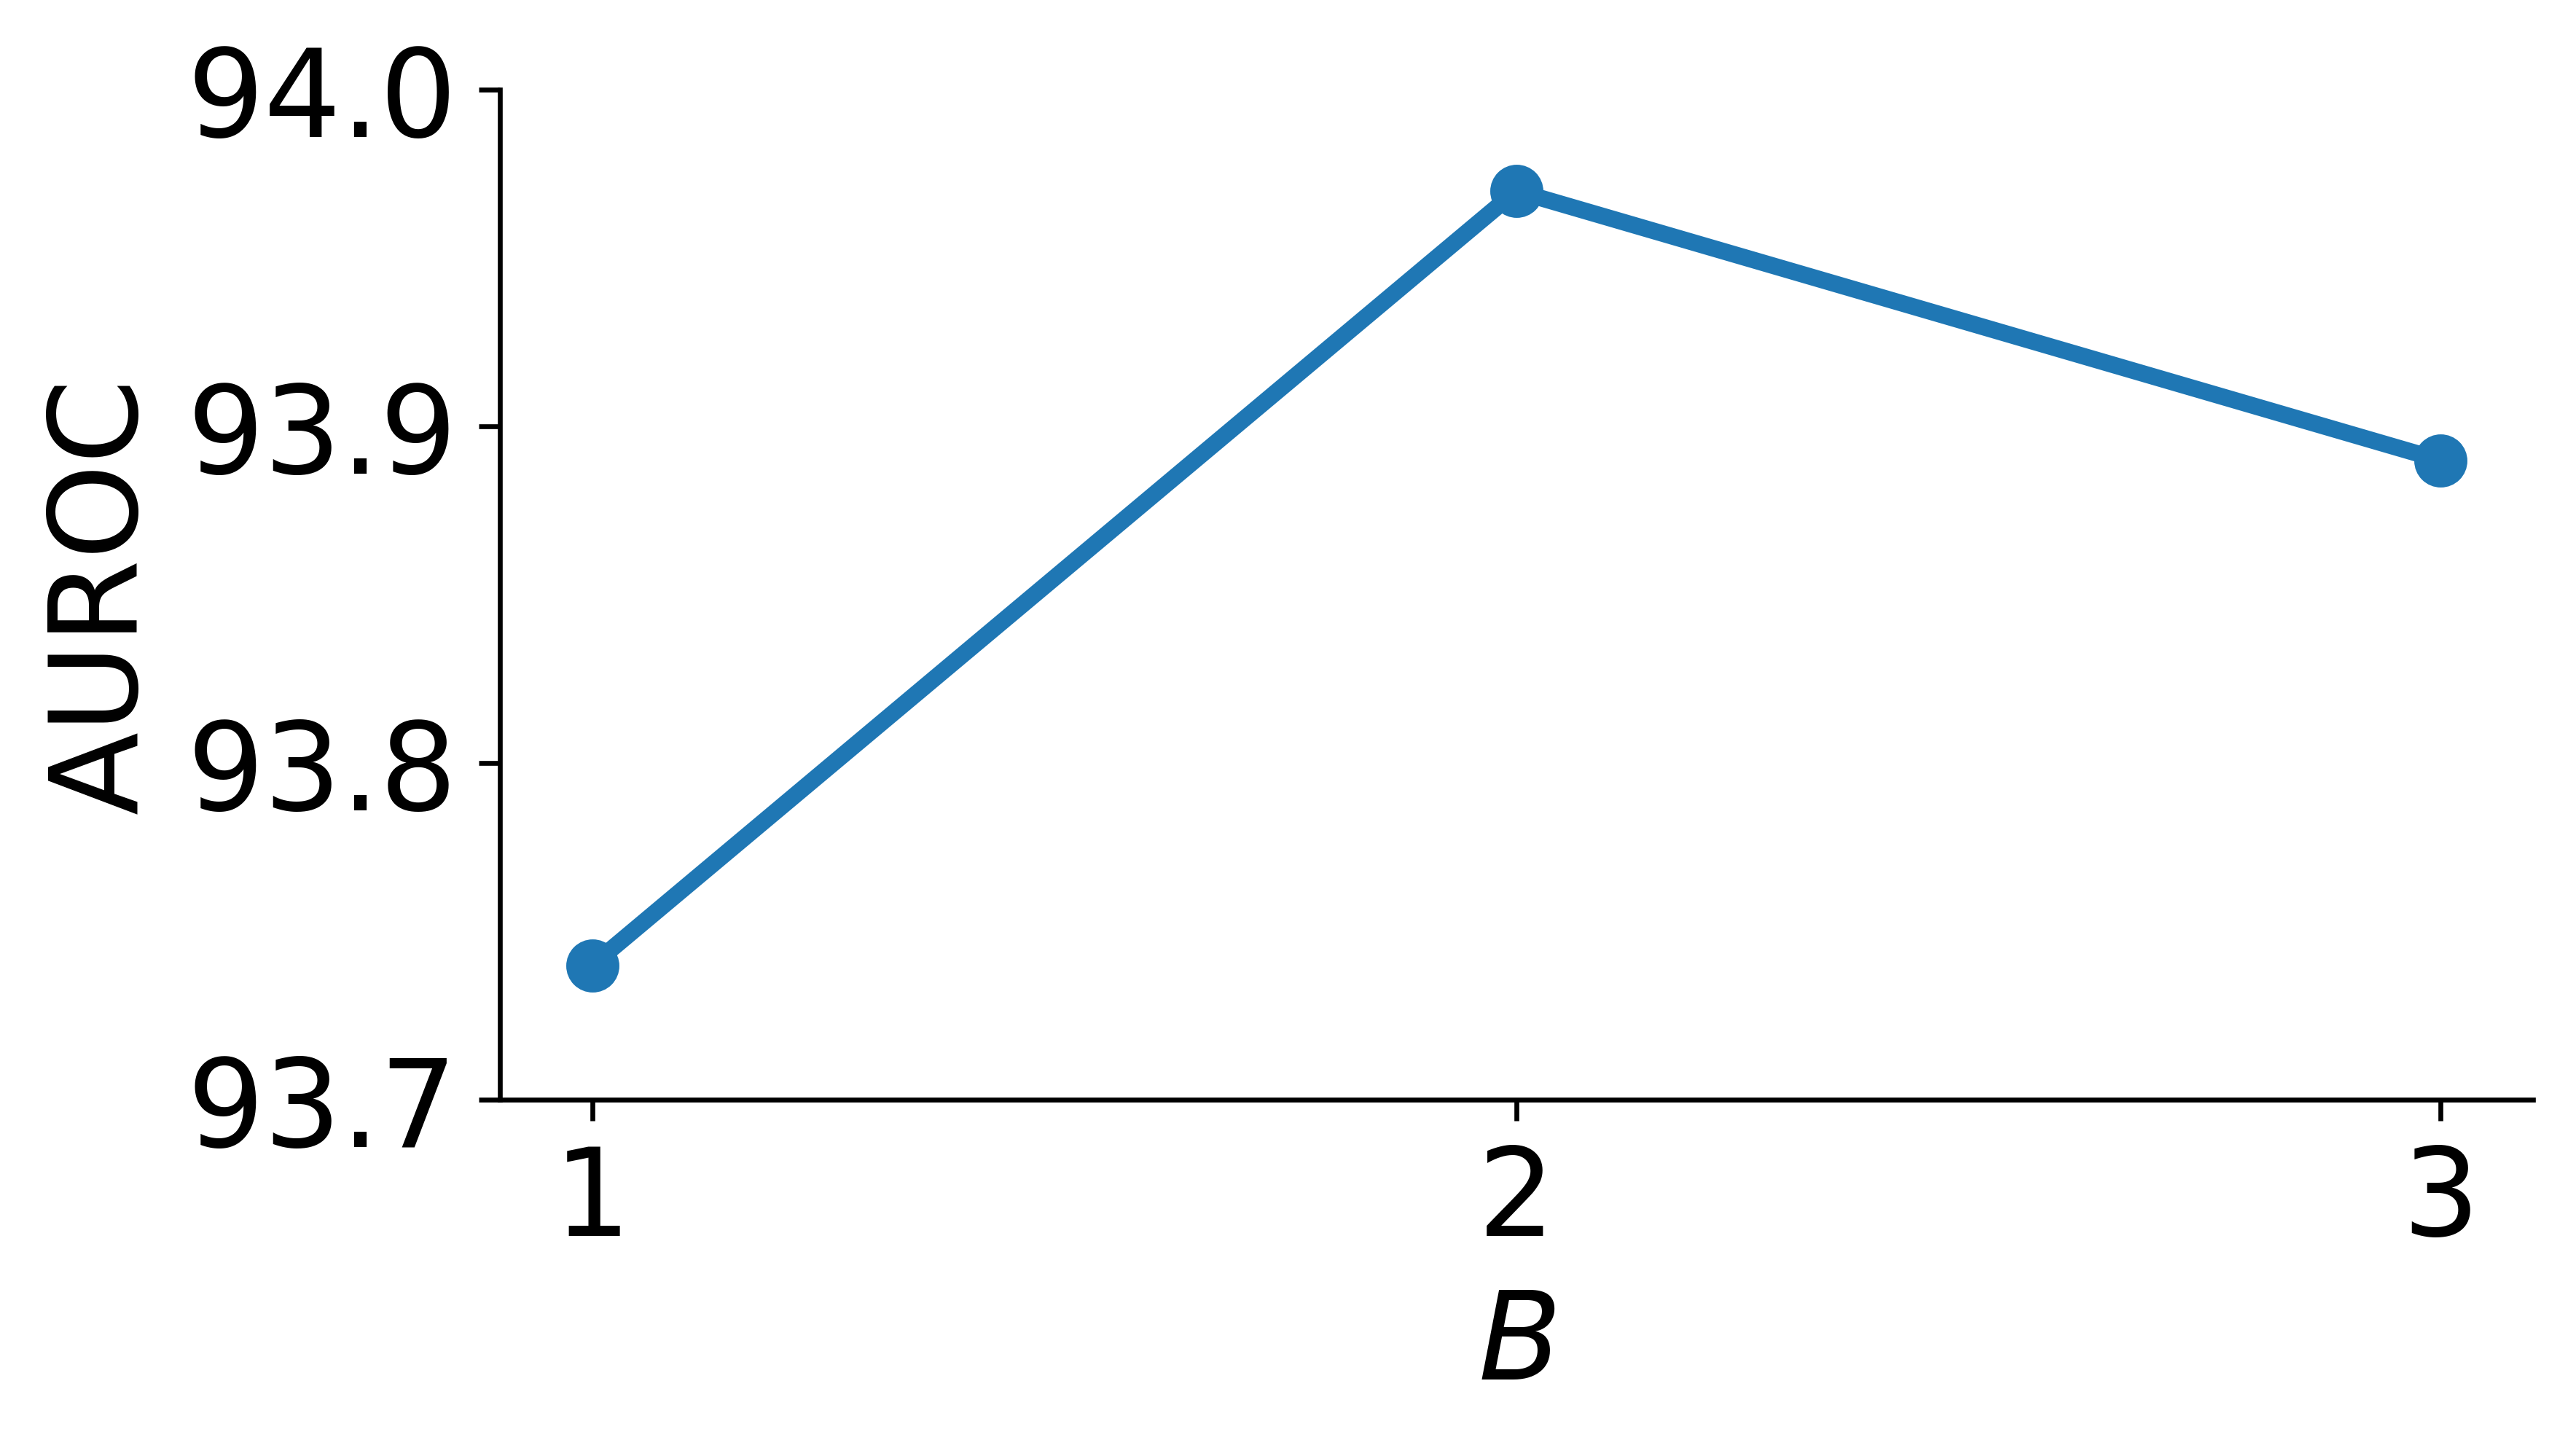
\includegraphics[width=0.55\linewidth]{figures/B_hparam_plot}
	\caption{Plot of \sys AUC against $B$.
	}
	\label{fig:blocks_hparam_plot}
\end{figure*}

%\textbf{Impact of $B$.} %To evaluate whether multi-layer cross-view feature fusion blocks (see Sec. \ref{sec:method-rep}) improve feature learning, 
%We experiment with a range of blocks $B = \{1, 2, 3\}$. Figure \ref{fig:blocks_hparam_plot} shows the average AUC trend for I-100-R ID. Using $B = 2$ blocks gives the highest AUC.% but the difference is minimal for small-scale datasets like I-100-R. %$B > 2$ blocks may be needed for more complex datasets, an investigation we leave for future research.
\subsubsection{Impact of the Number of Blocks}
The choice of number of blocks $B$ in \gls{cvca} affects the performance of \gls{sys}. To evaluate this effect on feature learning and OOD detection performance, an experiment was conducted over a range of blocks $B = \{1, 2, 3\}$. \ref{fig:blocks_hparam_plot} displays the average AUC trend for ImageNet-100 ID. $B = 2$ blocks results in the highest AUC performance from \gls{sys} but the difference is minimal for small-scale datasets like ImageNet-100. $B > 2$ blocks may be needed for more complex datasets.

\begin{table*}[htp!]
	%\small
	\centering
	\caption{ 
		Ablation OOD detection results (AUC, FPR) for ImageNet-100 ID comparing \sys to single-view models with equivalent data and equivalent parameters.%Results from 1 seed.
	}
\vspace{0.1cm}
	\scalebox{1.}{
		\begin{tabular}{|l|cccccc|}
			\hline
			%\multirow{2}{*}{} &  \multicolumn{6}{c|}{OOD}        \\ \cline{2-7} 
			%& Average (Far) & Average (Near) & Average \\ \hline
            & \multicolumn{2}{c}{Average (Far)} & \multicolumn{2}{c}{Average (Near)} & \multicolumn{2}{c|}{Average} \\ 
            & AUC$\uparrow$ & FPR$\downarrow$ & AUC$\uparrow$ & FPR$\downarrow$ & AUC$\uparrow$ & FPR$\downarrow$ \\ \hline
			Aug Base & 92.73 & 38.83 & 80.53 & 69.15 & 87.85 & 50.96  \\ 
			Fg-Bg Base & 92.70 & 38.88 & 80.51 & 69.10 & 87.83 & 50.97  \\ \cdashline{1-7}
			EqParam & 96.00 & 21.19 & 88.43 & 47.86 & 92.56 & 33.31  \\ \cdashline{1-7}
			%Rot-Noise & 95.74 & 16.06 & 87.28 & 46.06 & 90.90 & 28.06 \\
			%Crops & 95.74 & 19.87 & 87.40 & 45.44 & 90.97 & 30.10  \\  \hdashline
			\gls{sys} & 97.39 & 13.38 & 89.68 & 47.84 & 93.89 & 29.04  \\ \hline
		\end{tabular}
	}
	\label{tab:moredata_ablations_aug}
\end{table*}


%{\color{blue}
%\subsection{Comparison with Equivalent Data and Parameters}
%\label{sec:suppmat-eqparam}

%\textbf{Equivalent Augmented Data and Parameters.} One can argue that the comparison of \sys 
%with existing OOD baselines is unfair due to baselines 1) only using the original image while \sys uses the original image and its foreground and background views, and {\color{blue}2) having fewer learnable parameters than \sys}. %We note that this is an \textit{inherent property} of our proposed exploration, as we exploit multiple views for OOD detection performance benefits and design an effective framework to leverage it. Also, here, the additional views are generated automatically with an off-the-shelf toolkit and involve no explicit data collection effort. Furthermore, it has been shown that simply providing more data may not be enough in solving the OOD detection problem \cite{fang2022out}, attesting to the necessity of principled techniques such as \sys.
%Recent theoretical results show that simply providing more data is not enough to solve the OOD detection problem \cite{fang2022out}, attesting to the necessity of principled techniques such as \sys and establishing comparability between \sys and baselines. %Furthermore, our problem domain of using multiple views \textit{inherently necessitates more data} which we demonstrate can be efficiently processed with an off-the-shelf toolkit.
%
%%Despite this, we conducted two experiments where the baseline model is provided with the original image and two additional augmented images per sample to equalize the amount of training data between baselines and \sys. The augmentations chosen for the first experiment were based on findings indicating their benefit for OOD detection and include \textit{rotations} (from CSI \cite{tack2020csi}) and \textit{noise} (from random augmentation works \cite{cubuk2020randaugment}). %,hendrycks2022pixmix}). 
%%For the second experiment, we use the foreground and background views as the additional augmented images. The OOD detection results of these experiment on ID dataset I-100-R are presented in Table \ref{tab:moredata_ablations_aug} in rows ``Aug Base'' and ``Fg-Bg Base'' respectively. We chose the best-performing baseline OOD detection method, ViM, for comparison. \sys still outperforms baselines trained with equivalent data, showing that (1) cross-attention fusion of foreground-background views is key to improve OOD detection with segmented images, and (2) %our proposed \sys framework can effectively utilize such views, whose 
%%\sys performance benefits do not come from additional data. {\color{blue}We further consider the comparison between \sys and baseline models with equivalent number of parameters in Table \ref{tab:moredata_ablations_aug} (row ``EqParam'') and Appendix Sec. {\color{red}TODO}. \sys outperforms equivalent parameter baselines, showing the importance of CVCA fusion of multiple views.}
%We conduct experiments where the baseline model is 1) provided with two additional images per sample to equalize the amount of training data, and {\color{blue}2) provided the same number of parameters as \sys}. Results of these experiment on I-100-R ID are in Table \ref{tab:moredata_ablations_aug} in rows ``Aug Base'' (augmentations of the original image), ``Fg-Bg Base'' (segmented images used in \sys), and {\color{blue}``EqParam''. Details for the experiments are in Appendix Sec. E.3.} \sys still outperforms the baselines, showing that \sys performance gains do not come from additional resources and cross-attention fusion of foreground-background views is key to improve OOD detection with segmented images. %our proposed \sys framework can effectively utilize such views, whose 
%%.% {\color{blue}We further consider the comparison between \sys and baseline models with equivalent number of parameters in Table \ref{tab:moredata_ablations_aug} (row ``EqParam'') and Appendix Sec. {\color{red}TODO}. \sys outperforms equivalent parameter baselines, showing the importance of multiple view fusion.}
%
%Here we detail the experiments evaluating the performance of single-view baseline models when provided data and learnable parameters equivalent to those provided to \sys.
%
%\textbf{Equivalent Data.} Two experiments were conducted where the baseline model was provided with the original image and two additional augmented images per sample to equalize the amount of training data between baselines and \sys. The augmentations chosen for the first experiment were based on findings indicating their benefit for OOD detection and include \textit{rotations} (from CSI \cite{tack2020csi}) and \textit{noise} (from random augmentation works \cite{cubuk2020randaugment}). %,hendrycks2022pixmix}). 
%For the second experiment, we use the foreground and background views (used in \sys) as the additional augmented images. The OOD detection results of these experiment on ID dataset ImageNet-100-Random are presented in main paper Table 5 in rows ``Aug Base'' and ``Fg-Bg Base'' respectively. We chose the best-performing baseline OOD detection method, ViM, for comparison. \sys consistently outperforms baselines trained with equivalent data. This implies that the CVCA in \sys is key to improve OOD detection through fusion of the segmented foreground-background images. Furthermore, \sys performance benefits do not come from additional data.
\subsubsection{Comparison with Equivalent Data and Parameters}
\label{sec:suppmat-eqparam}
\gls{sys} utilizes multiple views of an image to perform OOD detection. A natural concern is that the performance of \gls{sys} is due to the use of additional data (three views as input instead of only one input, i.e. the original image) and additional parameters (three feature extractors and $\mathcal{U}$). This concern is unfounded because the problem inherently demands a different comparison. The nature of the multi-view OOD detection task implies the availability and necessary processing of additional data. The comparison to single-view baselines is out of necessity. Few previous multi-view OOD detection methods exist that are comparable to the methodology of \gls{sys}. \gls{sys}, comparatively, exploits multiple views for OOD detection by explicitly designing a framework to effectively leverage them. Furthermore, the additional views in multi-view OOD detection are not equivalent to additional data in the traditional sense presented in OOD detection literature. Each view is an augmentation of the original image and generated automatically (or already available) as part of the task setting, requiring no additional effort (e.g. data collection). Finally, it has been shown that solving the OOD detection problem fundamentally requires more than simply learning from or otherwise utilizing additional data \cite{fang2022out}. It is necessary to use principled techniques such as \gls{sys} in the presence of data to achieve state-of-the-art OOD detection, especially in the near-OOD domain.

Despite this, two additional experiments were conducted to evaluate the performance of \gls{sys} relative to baselines that 1) utilized additional data, and 2) utilized additional trainable parameters.
For the first experiment, a single-view baseline model was provided with two additional augmented images per sample (in addition to the original image), establishing an equal amount of training data between the baseline and \gls{sys} (Aug Base in \ref{tab:moredata_ablations_aug}). The augmentations chosen were inspired by established OOD detection works and include rotations (from CSI \cite{tack2020csi}) and noise (from random augmentation methods \cite{cubuk2020randaugment}). Additionally, a single-view baseline model was provided with the foreground and background segmented views along with the original view (Fg-Bg Base in \ref{tab:moredata_ablations_aug}). OOD detection results for \gls{sys} against these equivalent-data baseline for ImageNet-100 ID are in \ref{tab:moredata_ablations_aug}. Baselines used VIM. \gls{sys} outperforms baselines trained on equivalent data. This affirms that the performance increase with \gls{sys} is not from additional data but from an intelligent utilization of segmented views via \gls{cvca} fusion for OOD detection.

%{\color{blue}
%\textbf{Equivalent Parameters.} Another claim could be that \sys outperforms existing baselines due to the increase in parameters. To empirically verify that this is not the case, we conduct an experiment with a version of the single-view baseline model containing learnable parameters equivalent to those in \sys (i.e. 48M). The results on I-100-R ID are shown in Table \ref{tab:moredata_ablations_aug}. Even with more parameters, the baselines do not outperform \sys, indicating that the view fusion mechanisms introduced by \sys are critical to improved performance instead of the parameter increase. {\color{red}move to Appendix and explain why this difference doesn't matter, models will have different sizes, changing pretrained model/backbone is very unfair - our method proposed the FF not the backbone, we still outperform; MAKE SURE THIS IS IN THE REBUTTAL AS WELL}
%}
%
%\textbf{Equivalent Parameters.} Another claim could be that \sys outperforms existing baselines due to the increase in parameters. To empirically verify that this is not the case, we conduct an experiment with a version of the single-view baseline model containing learnable parameters equivalent to those in \sys (i.e. 48M). The results on ID dataset ImageNet-100-Random are shown in main paper Table 5. Even with more parameters, the baselines do not outperform \sys, indicating that the view fusion mechanisms introduced by \sys are critical to improved performance instead of the parameter increase.
%
%We note that changing the feature extraction backbone for the single-view baseline (i.e. by increasing the number of learnable parameters) but not for \sys is an unfair comparison. A significant amount of the learnable parameters (28.67 MiB) in \sys are in the feature fusion head, which is designed to be modular to patch-based feature extraction backbones. The intuitive decision when presented with a superior feature extraction backbone would be to use it with our proposed feature fusion head, thus re-establishing a fair comparison with \textit{equivalent feature extractors}. Nevertheless, \sys still outperforms the single-view baseline with equivalent parameters despite using weaker feature extraction backbones. %{\color{red}move to Appendix and explain why this difference doesn't matter, models will have different sizes, changing pretrained model/backbone is very unfair - our method proposed the FF not the backbone, we still outperform; MAKE SURE THIS IS IN THE REBUTTAL AS WELL}
%}
For the second experiment, a single-view baseline model was expanded in each layer dimension such that the final trainable parameter count was equivalent to those in \gls{sys} (i.e. 48M). The results comparing OOD detection performance between \gls{sys} and the equivalent-parameter baseline on ImageNet-100 ID are in \ref{tab:moredata_ablations_aug} (EqParam row). Despite the additional parameters available to the single-view baseline, \gls{sys} still outperforms baseline methods. This further establishes that the performance improvements evidenced by \gls{sys} are not from an increased amount of trainable parameters. The mechanisms in \gls{sys}, such as leveraging of multi-view data and CVCA feature fusion, are critical to the improved OOD detection displayed by \gls{sys}.

This comparison is additionally valuable because it reiterates an important discrepancy across ML and commonly compared against in OOD detection. Changing the sizes of feature extraction backbones in baselines, e.g. by increasing the amount of trainable parameters but not for \gls{sys}, is an illogical and irreconcilable comparison. The existence of such a backbone could be used directly in \gls{sys} as the trainable parameters and contributions of \gls{sys} are not from the feature extraction backbones (which are simply pre-trained models used directly from source). \gls{sys} uses LoRA adapters and $\mathcal{U}$ on top of such pre-trained backbones. In fact, a significant mount of trainable parameters in \gls{sys} (28.67 MiB) are in the fusion component $\mathcal{U}$, which is modular to any patch-based feature extraction backbone. Intuitively, any superior feature extraction backbone (e.g. one with increased parameters as described above) would simply be used with the LoRA adapters and $\mathcal{U}$ in a complementary relationship. Establishing a comparison between different feature extraction backbones in \gls{sys} and a baseline is both meaningless from a practical standpoint and unfair from the perspective of scientific evaluation. Nevertheless, \gls{sys} remains superior over single-view baselines despite the difference in parameters between feature extraction backbones.

%{\color{purple} The Table 5 results were included together to save space in the draft. We will separate the Aug Base comparison from the Split and Crops comparisons in our revision. We further evaluated baselines with the suggested foreground and background augmentations and found them to be weaker than COD. Results are below and we will include them in our revision. Experiment setting is ImageNet-100-Random.
%	
%	Fg-Bg Baseline: 80.51\%, 92.70\%, 87.83\% \\
%	COD (ours): 89.07\%, 97.24\%, 93.97\% \\
%}

%\begin{table*}[htp!]
%	%\small
%	\centering
%	\caption{ 
%		Ablation OOD detection results (AUC, FPR) for ImageNet-100 ID for \sys with different post-hoc OOD detection methods.
%	}
%	\vspace{0.15cm}
%	\scalebox{0.9}{
%		\begin{tabular}{|l|cccccc|}
%			\hline
%		%\multirow{2}{*}{} &  \multicolumn{6}{c|}{OOD}        \\ \cline{2-7} 
%		%& Average (Far) & Average (Near) & Average \\ \hline
%        & \multicolumn{2}{c}{Average (Far)} & \multicolumn{2}{c}{Average (Near)} & \multicolumn{2}{c|}{Average} \\ 
%        & AUC$\uparrow$ & FPR$\downarrow$ & AUC$\uparrow$ & FPR$\downarrow$ & AUC$\uparrow$ & FPR$\downarrow$ \\ \hline
%			MSP & 90.77 & 49.45 & 84.77 & 65.55 &  87.77 & 57.50 \\ 
%			KNN & 93.30 & 36.66 & 75.05 & 82.37 & 84.18 & 59.52  \\ \hdashline
%			\sys-MSP & 92.60 & 35.30 & 89.01 & 48.93 & 90.07 & 41.49  \\ 
%			\sys-KNN & 95.35 & 24.38 & 88.17 & 55.83 & 92.08 & 38.67  \\ \hdashline
%			\sys & 97.31 & 13.49 & 89.16 & 47.76 &  93.24 & 30.63 \\ \hline
%		\end{tabular}
%	}
%	\label{tab:ab_othermethods}
%	\vspace{-0.1cm}
%\end{table*}
%{\color{blue}
%\subsection{Segmented Foreground-Background Quality and Domain Shift}
%\label{sec:suppmat-fgbgqualds}

%\textbf{Augmented Views.} Rotations and noise image augmentations have been shown to improve OOD detection \cite{tack2020csi,cubuk2020randaugment}. We experiment with training \sys with a rotated image and a noisy image instead of segmented views. % to investigate if such augmentations are sufficient for improved OOD detection. 
%Results for I-100-R ID are in Table \ref{tab:moredata_ablations_aug} (``Rot-Noise''). \sys with segmented views is superior to using augmentations.%, verifying the usefulness of the segmented feature information.

%\textbf{Effect of Foreground-Background Quality.} We investigate if the performance benefits of \sys are reliant on properly segmented foregrounds and backgrounds. For this, we perform two evaluations.

%%For evaluation (1), we generate two additional datasets with poor semantic correlation across views: each view contains half of the image split vertically (``Split''), and one view contains off-center crops of the image while the other view contains the rest of the image (``Crops''). Results of this experiment on ID dataset I-100-R are presented in Table \ref{tab:moredata_ablations}. %in rows ``Split'' and ``Crops''. 
%First, we evaluate \sys with improperly separated foregrounds and backgrounds. Results of this experiment on I-100-R ID are presented in Table \ref{tab:moredata_ablations_aug} in row ``Crops'' (details in Appendix Sec. E.4).
%\sys with foreground-background views outperforms poor segmentation views, indicating that \sys improves with increasingly semantically meaningful segmentation. {\color{blue}This is supported in further experiments with a weaker segmentation model (see Appendix Sec. E.5).} % for optimal discriminative feature learning and OOD detection. %\textcolor{red}{answer: why is Rot-Noise worse than Crops? shouldn't random Crops be worse?} \alex{potential reason - existing work in e.g. jigsaw augmentations gives good results for OOD detection, random crops simulates this just in two different views}
%
%We provide details for our investigation into if \sys performance benefits originate in properly segmented foregrounds and backgrounds. For this, two questions are asked:
%\begin{enumerate}
%    \item Does \sys require properly separated foregrounds and backgrounds?
%    \item Can \sys still perform well across datasets of varying separation quality?
%\end{enumerate}
%
%For (1), we generate an additional dataset with poor semantic correlation across views: one view contains off-center crops of the image while the other view contains the rest of the image (``Crops''). Results of this experiment on ID dataset ImageNet-100-Random are presented in main paper Table 5. 
%\sys with the poor segmentation-quality dataset is weaker than \sys with foreground-background segmentation. This demonstrates that increasingly semantically meaningful foregrounds and backgrounds directly improve the performance of \sys. 
%
\subsubsection{Segmented Foreground-Background Quality and Domain Shift}
\label{sec:suppmat-fgbgqualds}

An important question is if the performance benefits of \gls{sys} stem from properly segmented foreground and background views. This question is complex and requires analysis across a range of segmentation quality, both from the perspective of the segmentation procedure itself and from the perspective of domain shift.

\begin{table*}[htp!]
	%\small
	\centering
	\caption{ 
		Ablation OOD detection results (AUC, FPR) on ImageNet-100 ID using the original image and two additional synthetic views instead of foreground-background segmented views. %Results from 1 seed.
	}
\vspace{0.1cm}
	\scalebox{1.}{
		\begin{tabular}{|l|cccccc|}
			\hline
			%\multirow{2}{*}{} &  \multicolumn{6}{c|}{OOD}        \\ \cline{2-7} 
			%& Average (Far) & Average (Near) & Average \\ \hline
            & \multicolumn{2}{c}{Average (Far)} & \multicolumn{2}{c}{Average (Near)} & \multicolumn{2}{c|}{Average} \\ 
            & AUC$\uparrow$ & FPR$\downarrow$ & AUC$\uparrow$ & FPR$\downarrow$ & AUC$\uparrow$ & FPR$\downarrow$ \\ \hline
			Rot-Noise & 95.74 & 16.06 & 87.28 & 46.06 & 90.90 & 28.06 \\
			Crops & 95.74 & 19.87 & 87.40 & 45.44 & 90.97 & 30.10  \\  \cdashline{1-7}
			\gls{sys} & 97.39 & 13.38 & 89.68 & 47.84 & 93.89 & 29.04  \\ \hline
		\end{tabular}
	}
	\label{tab:moredata_ablations_views}
\end{table*}

First, the presence of properly separated foregrounds and backgrounds is evaluated using two alternative multi-view datasets with \gls{sys}. The first dataset uses the aforementioned data augmentations of rotations and noise as the ``foreground'' and ``background'' views to evaluate the performance of \gls{sys} when provided with views that are not segmented at all (Rot-Noise). The second dataset uses one view with off-center crops of the original image and the other view containing the rest of the original image (Crops). This evaluates the performance of \gls{sys} under poor semantic correlation across views. Results of \gls{sys} with these alternative multi-view datasets for ImageNet-100 ID are presented in \ref{tab:moredata_ablations_views}. \gls{sys} trained and tested on datasets with poor segmentation quality is less capable in OOD detection compared to \gls{sys} with foreground and background segmented views. This implies that \gls{sys} extracts significantly more discriminative features via \gls{cvca} from semantically meaningful foregrounds and backgrounds.

\begin{table*}[htp!]
%\small
\centering
\caption{
	Ablation OOD detection results (AUC, FPR) using ID training datasets of varying separation quality and object-domain relevance: Textures (low separation quality) and NINCO (clear separation but multiple complex objects in the foreground)
	. %Results from 1 seed. 
	Note that Textures has no known near-OOD datasets, the datasets are simply evaluated together. (b) denotes results using a baseline model.
}
\vspace{0.1cm}
\scalebox{1.}{
	\begin{tabular}{|l|cccccc|}
		\hline
		%\multirow{2}{*}{} &  \multicolumn{6}{c|}{OOD}        \\ \cline{2-7} 
		%& Average (Far) & Average (Near) & Average \\ \hline
        & \multicolumn{2}{c}{Average (Far)} & \multicolumn{2}{c}{Average (Near)} & \multicolumn{2}{c|}{Average} \\ 
        & AUC$\uparrow$ & FPR$\downarrow$ & AUC$\uparrow$ & FPR$\downarrow$ & AUC$\uparrow$ & FPR$\downarrow$ \\ \hline
		Textures (b) & \slash & \slash & \slash & \slash & 95.94 & 19.05  \\ 
		(\gls{sys}) & \slash & \slash & \slash & \slash & 96.61 & 14.73  \\ \cdashline{1-7}
		NINCO (b) & 80.62 & 60.03 & 95.65 & 20.38 & 84.37 & 50.12 \\ 
		(\gls{sys}) & 88.61 & 44.61 & 92.85 & 30.06 & 89.67 & 40.97  \\ \hline
	\end{tabular}
}
\label{tab:segqual_ablations}
\end{table*}

%Second, we evaluate \sys across datasets of varying separation quality {\color{blue}due to domain shift, i.e. when the ID and OOD data include fewer object features which the YOLOv5 segmentation model was trained on (i.e. COCO) \cite{jocher2020ultralytics}.} We select the non-ImageNet datasets of Textures, NINCO, {\color{blue}and a medical dataset} as ID datasets (details in Appendix Sec. E.4). Results in Table \ref{tab:segqual_ablations} and Appendix Sec. E.4 indicate that \sys trained with varying foreground-background separation quality {\color{blue}and domain shift} \textit{still achieves superior OOD detection performance}. This shows that \sys is robust to foreground-background quality from domain shift.  % and further that the proposed cross-view attention is critical to learning discriminative features in images. 
%%These results also show that \sys is not tightly coupled to the ID training dataset nor the segmentation tool as both Textures and NINCO are mutually exclusive to ImageNet.% and DUTS-TR.
%
%For (2), we select non-ImageNet datasets with varying foreground-background separation quality as ID data. The Textures dataset does not have clear foreground objects and we use it to evaluate \sys performance when ID training data foregrounds and backgrounds are poorly separated. Furthermore, we evaluate \sys with NINCO as ID because it includes complex samples with foregrounds containing multiple objects. With Textures as the ID dataset, we use I-30, iNaturalist, Places, NINCO, SUN, OpenImage-O, Species, SSB-HARD, and Food as OOD datasets. For Textures, \sys was trained using settings identical to those of ImageNet-100-Random. With NINCO as the ID dataset, we use I-30, SSB-HARD, and Food as near-OOD datasets and Textures, iNaturalist, Places, SUN, OpenImage-O, and Species as far-OOD datasets. We trained \sys to convergence with a LoRA rank of 16. All other training and model configurations were identical to the ImageNet-100-Random experiment settings. Results in main paper Table 7 indicate that \sys is robust to foreground-background segmentation quality during training. Despite the varying quality of features in the views, \sys still outperforms baselines and comparison points. Furthermore, the results reinforce that the proposed cross-view attention is critical to learning discriminative features in images. 
Second, the efficacy of \gls{sys} is evaluated when presented with foreground-background views of varying segmentation quality. Non-ImageNet datasets are selected and segmented into foregrounds and backgrounds. The Textures dataset was selected as a low segmentation quality dataset as it does not have clear foreground objects. This evaluates the performance of \gls{sys} when presented with poorly separated views. The NINCO dataset was selected as a medium segmentation quality dataset as it contains complex images with multiple foreground objects. This evaluates the performance of \gls{sys} when presented with views containing noisy features or spurious features in the views. For Textures as the ID dataset, I-30, iNaturalist, Places, NINCO, SUN, OpenImage-O, Species, SSB-HARD, and Food were used as OOD datasets. For NINCO as the ID dataset, I-30, SSB-HARD, and Food were used as near-OOD datasets and Textures, iNaturalist, Places, SUN, OpenImage-O, and Species were used as far-OOD datasets. For both datasets, \gls{sys} was trained using settings identical to those of ImageNet-100 with the exception of NINCO which used a LoRA rank of 16. Results for \gls{sys} with datasets of varying foreground-background separation quality are presented in \ref{tab:segqual_ablations}. \gls{sys} is robust to foreground-background segmentation quality, outperforming baselines despite the quality of the view features. This further isolates the source of performance benefits from \gls{sys} to the proposed \gls{cvca} feature fusion architecture. Given somewhat correlated foreground-background views, the feature fusion component in \gls{sys} can leverage the discriminative features within and across views to learn a feature space conducive to OOD detection.

%%{\color{red}medical data - severe domain shift}
%{\color{blue}
%\textbf{\sys under Domain Shift.} We consider the performance of \sys under domain shift, i.e. when ID and OOD data do not include objects which the YOLOv5 segmentation model was trained on (i.e. COCO) \cite{a}. Results on Textures (Table \ref{tab:segqual_ablations}) show that \sys is robust to a domain shift from objects to textures. A further evaluation on medical data (severe domain shift) shows an average AUC for \sys of 79.93\% against a baseline AUC of 79.78\%. \sys weakens under severe domain shift but still slightly outperforms the baseline. Details for this study are in Appendix Sec. {\color{red}TODO}.
%%The selected segmentation model for \sys was YOLOv5, which is trained on a dataset with 80 clear object classes (i.e. COCO) \cite{a}. However, tasks may not always involve object data, exhibiting domain shift. The results on NINCO (fine-grained objects, little domain shift) and Textures (textures with no clear objects, moderate domain shift) as ID datasets from the previous section (Table \ref{tab:segqual_ablations}) indicates that \sys is also robust to domain shift.
%
%%To further evaluate \sys under severe domain shift, we additionally experiment with a medical dataset that is very different from COCO. Details on datasets and results can be found in Appendix Sec. {\color{red}TODO}). The average AUC performance of \sys is 79.93\% while the closest baseline is 79.78\%. \sys weakens under severe domain shift but still slightly outperforms the baseline. We hypothesize that this is due to the preservation of the original view ensuring at least the learned knowledge of single-view models.
%}
%
%\textbf{Domain shift.} Segmentation quality can also be used as a basis for analysis into the performance of \sys under domain shift. The selected segmentation model for \sys was YOLOv5, which is trained on an object dataset (i.e. COCO) \cite{jocher2020ultralytics}. However, tasks may not always involve object data. We investigate the performance of \sys under \textit{domain shift}, that is when the ID and OOD data contain fewer or unclear object features. The results on NINCO and Textures as ID datasets indicates that \sys is also robust to domain shift. NINCO is similar to COCO and \sys performs well. Textures contains images of textures, not objects \cite{cimpoi2014describing}, and thus exhibits domain shift from COCO which contains 80 classes of clear objects \cite{lin2014microsoft}. \sys still performs well, although the performance gap is smaller with respect to the baseline.
%
%To evaluate \sys under severe domain shift, we additionally experiment with a medical dataset that is very different from COCO. Specifically, we use the MEL, NV, BCC, AK, and DF classes from the ISIC 2019 dataset \cite{codella2018skin} as ID and the BKL, VASC, and SCC classes from the ISIC 2019 dataset as well as 2000 randomly selected samples from the NCT dataset \cite{kather2018100} as OOD \cite{narayanaswamy2023exploring}. The average AUC performance of \sys is 79.93\% while the closest baseline is 79.78\%. \sys still slightly outperforms the baseline under severe domain shift, likely due to the preservation of the original view ensuring at least the learned knowledge of single-view models.
%}
Third, \gls{sys} is evaluated in a setting exhibiting extreme domain shift. That is, the data presented to \gls{sys}, and more specifically to the segmentation model used to generate the foregrounds and backgrounds subsequently leveraged by \gls{sys}, is completely different (i.e. drawn from a different distribution) from what was previously seen. This implies both covariate and semantic domain shifts which introduce significant deviations from learned knowledge, potentially resulting in unreliable performance. Specifically, the segmentation model used, YOLOv5, was pre-trained on a COCO, a dataset with 80 clear object classes \cite{jocher2020ultralytics}. Domain shift relative to COCO implies data with few or unclear object features.

The previous results of \gls{sys} on Textures as ID data indicate that \gls{sys} is robust to moderate domain shift, as Textures data does not contain any objects \cite{cimpoi2014describing}. To more thoroughly evaluate \gls{sys} with respect to heavy domain shift, a medical dataset was selected to test \gls{sys} with segmented data significantly different than the object data seen in COCO. The MEL, NV, BCC, AK, and DF classes from the ISIC 2019 dataset \cite{codella2018skin} were used as the ID dataset, and the BKL, VASC, and SCC classes from the ISIC 2019 dataset were used with 200 randomly selected samples from the NCT dataset \cite{kather2018100} as the OOD dataset \cite{narayanaswamy2023exploring}. Average AUC from \gls{sys} in this heavy domain shift experimental setting is 79.93\% while the closest baseline is 79.78\%. Despite the significantly modified data distributions and resulting segmented foreground-background views, \gls{sys} slightly outperforms baselines. It is hypothesized that this is due to the preservation of the information in the original image, allowing \gls{sys} to at least learn the original view features and achieve baseline OOD detection performance. This also implies that \gls{sys} may learn to ignore spurious view features if they do not contain discriminative feature information relative to the ID classes.

%{\color{blue}
%\subsection{Importance of Segmentation Model}
%\label{sec:suppmat-domshift}

%To further investigate the importance of segmentation model in \sys, we experiment with a U2-Net pre-trained on the DUTS-TR \cite{wang2017learning} dataset. We use ImageNet-100-Random for ID and Textures and NINCO for OOD. To ensure fairness, we remove all overlapping data between DUTS-TR and the ID and OOD datasets. The average AUC and FPR results for \sys with U2-Net is 83.51\% (AUC) and 63.63\% (FPR) while \sys (with YOLOv5) is 96.14\% (AUC) and 20.39\% (FPR). The older U2-Net is simultaneously slower at segmentation (taking about 0.8 seconds per image) and weaker than YOLOv5 at OOD detection. Qualitative analysis showed that U2-Net often segmented foreground objects correctly but frequently included spurious background features, thus diluting the discriminative features.
%
%Following recent trends in OOD detection literature using pre-trained vision-language models (VLMs) (e.g. CLIP \cite{radford2021learning}) \cite{miyai2024locoop,li2025synthesizing,jiang2024negative}, we investigate using the vision backbone from pre-trained CLIP as the feature extractor in \sys. The results are in Table \ref{tab:clip_ablation}. \sys with ViT and LoRA feature extractor backbones outperforms \sys with CLIP vision feature extractor backbones. \sys with LoRA adds additional learning capacity to the model, allowing it to learn to extract more discriminative features during training. Additionally, CLIP typically also uses \textit{text data} which is not considered in our domain. This simultaneously shows the reliance on CLIP-based OOD detection methods on text inputs as well as image inputs and demonstrates that VLM-based methods have certain limitations that prevent them from being directly translated to the image-only domain. Overall, we consider this to be an invalid comparison as 1) CLIP relies on text data while we do not, and 2) CLIP has likely seen some of the ID and OOD data before during pre-training, leading to information leakage. There is evidence for this in the literature, with CLIP achieving extremely high zero-shot OOD detection performance \cite{esmaeilpour2022zero}. \sys overcomes this challenge through our proposed view fusion method.
%}

%However, to more accommodate recent trends in OOD detection using VLMs, we try using the pretrained CLIP vision backbone in our method and include results in the Appendix (sec. E.5, pg. 9, start line 487). %The results on ImageNet-100-Random are below (AUROC; mean near-OOD, mean far-OOD, mean overall): 
%%\begin{itemize}
%%    \item CASOD-CLIP: 85.90\%, 93.48\%, 90.04\%
%%    \item \underline{CASOD}: 89.68\%, 97.39\%, 93.89\%
%%\end{itemize}
%CLIP underperforms compared to CASOD. We suspect this is due to the fact that our LoRA backbones in CASOD add additional learning capacity. This further shows that VLM-based OOD detection methods using CLIP make use of text data to improve performance while our proposed view fusion method is necessary in the image-only domain.
\subsubsection{Importance of Segmentation Model}
\label{sec:suppmat-altsegmod}

Expanding on the previous section, the performance of \gls{sys} with different segmentation models is considered as a natural subsequent evaluation. Instead of YOLOv5, two additional segmentation models % from varying pre-trained distributional relevance to the ID data considered by \gls{sys} 
are considered. First, a U2-Net pre-trained on the DUTS-TR dataset \cite{wang2017learning} is used. All overlapping data between the DUTS-TR dataset and ImageNet-100 setting ID and OOD datasets is removed to ensure fairness in the evaluation. As DUTS-TR is also an object dataset, the data semantic and covariate distributions are similar to that of YOLOv5. However, the U2-Net architecture is significantly older (and thus weaker) than that used by YOLOv5, resulting in a dissimilar data distribution for the resultant foreground and background views. Using ImageNet-100 for the ID dataset and Textures and NINCO for the OOD datasets, \gls{sys} results in an AUC of 83.51\% and FPR95 of 63.63\% using views from U2-Net. Compared to an AUC of 96.14\% and FPR95 of 20.39\% using views from YOLOv5, it is clear that the segmentation model (and resulting segmentation quality) impacts the performance of \gls{sys}. This follows the observations from the previous ablation studies and further illuminates the relevance of foreground-background view segmentation from the perspective of object separation quality (as embodied by the segmentation model pre-training). Furthermore, U2-Net is slower than YOLOv5, requiring about 0.8 seconds per image to perform foreground-background segmentation. Qualitative analysis of the images segmented by U2-Net revealed that foreground objects were often correctly isolated but frequently contained spurious background features. This diluted the discriminative features in views and degraded feature learning and subsequent OOD detection performance.

\begin{table*}[htp!]
	\small
	\centering
	\caption{ 
		Ablation OOD detection results (AUC) for ImageNet-100 ID between \sys with LoRA ViT feature extractor backbones and \sys with CLIP vision feature extractor backbone. %Results from 1 seed.
	}
\vspace{0.1cm}
	\scalebox{1.}{
		\begin{tabular}{|l|ccc|}
			\hline
			\multirow{2}{*}{} &  \multicolumn{3}{c|}{OOD}        \\ \cline{2-4} 
			& Average (Far) & Average (Near) & Average \\ \hline
			\gls{sys}-CLIP & 93.84 & 85.90 & 90.04  \\
			\gls{sys} & 97.39 & 89.68 & 93.89  \\ \hline
		\end{tabular}
	}
	\label{tab:clip_ablation}
\end{table*}

Recent OOD detection literature has focused on exploring the potential of pre-trained Vision Language Models (VLMs) \cite{miyai2024locoop,li2025synthesizing,jiang2024negative}, such as CLIP \cite{radford2021learning}. To account for this recent trend, \gls{sys} is additionally evaluated using the vision backbone from a pre-trained CLIP model as the feature extractor backbone (and including $\mathcal{U}$, adding LoRA to the CLIP model components is non-trivial and attempts led to significant performance decreases). The results on ImageNet-100 ID between \gls{sys} with ViT backbone and CLIP backbone (\gls{sys}-CLIP) are presented in \ref{tab:clip_ablation}. \gls{sys}-CLIP is worse than \gls{sys} in OOD detection. The embodied knowledge and additional learning capacity from the ViT backbone and LoRA components respectively enable significantly improved feature learning from \gls{sys} over \gls{sys}-CLIP which must rely more on the pre-trained abilities of the CLIP vision backbone. Importantly, CLIP is designed to leverage images and text data, but text data is not allowed in the considered OOD detection task. This reveals two observations. First, that CLIP relies on text inputs as well as image inputs for functionality, including OOD detection. Second, that CLIP-based OOD detection methods have limitations that prevent them from being translated to the image domain, which may be a negative consideration in applications. In summary, this is an invalid comparison both for the above reasons and because CLIP is pre-trained on a vast amount of data. This raises the likelihood that CLIP has already encountered some of the ID and OOD data presented during training and testing, a significant source of information leakage and a complete invalidation of scientific reliability. There is evidence for this leakage in literature, with CLIP exhibiting zero-shot OOD detection performance \cite{esmaeilpour2022zero}.

\begin{table*}[htp!]
	\small
	\centering
	\caption{ 
		Ablation OOD detection results (AUC) for ImageNet-100-Random ID between \sys and \sys when trained without individual view feature losses ($\mathcal{L}_{CE,fused}$ only). %Results from 1 seed.
	}
\vspace{0.1cm}
	\scalebox{1.}{
		\begin{tabular}{|l|ccc|}
			\hline
			\multirow{2}{*}{} &  \multicolumn{3}{c|}{OOD}        \\ \cline{2-4} 
			& Average (Far) & Average (Near) & Average \\ \hline
			$\mathcal{L}_{CE,fused}$ only & 97.05 & 88.19 & 93.50  \\
			\gls{sys} & 97.39 & 89.68 & 93.89  \\ \hline
		\end{tabular}
	}
	\label{tab:nomvloss_ablations}
\end{table*}

%We additionally investigated \sys using \textit{only} the fused feature CE loss $\mathcal{L}_{CE,fused}$, i.e. $\mathcal{L}_{CE} = \mathcal{L}_{CE,fused}$. The OOD detection AUC results for ID dataset ImageNet-100-Random are presented in Table \ref{tab:nomvloss_ablations}. Training with only the final fused feature reduces overall performance. This is primarily because including the individual view CE loss terms encourages learning of more diverse class discriminative features in each of the corresponding views. As the features in these views are different, the resulting individual view features contain more diverse discriminative information for feature fusion. This is particularly noticeable in the increase in near-OOD performance relative to far-OOD performance. Learning more discriminative features improves detection of challenging near-OOD samples, closing the gap for \sys to \textbf{4.21\%} from 5.31\% for \sys with only fused feature CE loss.
\subsubsection{Individual View Loss Contribution}
\label{sec:suppmat-nomvloss}

\gls{sys} uses a combination of a fused feature CE loss and individual view feature CE losses to learn ID class-relevant discriminative features during training (see Section \ref{sec:casod_method-train}). To investigate if these loss components are necessary, the performance of \gls{sys} when trained using only the fused feature CE loss $\mathcal{L}_{CE,\mathcal{U}}$, i.e. $\mathcal{L}_{CE} = \mathcal{L}_{CE,\mathcal{U}}$, was evaluated. OOD detection results with ImageNet-100 ID are in \ref{tab:nomvloss_ablations}. Without including the individual view feature CE losses, performance decreases. The loss terms for the individual view features encourage learning of class discriminative features in each corresponding view, increasing feature diversity at the feature fusion stage. As each view contains different information, learning within these views increases the representation of features beneficial for learning in subsequent \gls{cvca} feature fusion operations. This benefit is clear in the near-OOD performance. The gap between near-OOD and far-OOD detection using \gls{sys} with individual view feature CE losses is 4.21\% while it is 5.31\% without individual view feature CE losses. This reduction in performance discrepancy implies a reliance on individual view features for OOD detection in \gls{sys}. 

%\begin{table*}[t!]
%	\small
%	\centering
%	\caption{\textbf{OOD Results for \sys and different OOD methods}: \textit{near-OOD} detection (\textbf{AUC}) comparison between \sys using MD (\sys), \sys using MSP (\sys-MSP), and \sys using KNN (\sys-KNN). %
%	}
%	\scalebox{0.725}{
%		\begin{tabular}{|l|ccccc|c|cccccc|c|c|}
%			\hline
%			\multirow{2}{*}{} &  \multicolumn{14}{c|}{ID data: ImageNet-100-Random}  \\ \cline{2-15}
%			& I-30 & I-900  & NINCO & SSB-Hard & Food & Avg. - Near & Textures  & iNaturalist  & Places  & SUN & OpenImage-O & Species & Avg. - Far & Avg. \\ \hline
%            MSP    & 83.55 & 85.44 & 89.54 & 85.16 & 80.18 & 84.77 & 92.71 & 94.17 & 88.41 & 86.96 & 92.65 & 89.73 & 90.77 & 88.04 \\
%            KNN    & 77.32 & 78.33 & 80.57 & 73.28 & 65.76 & 75.05 & 96.10 & 80.39 & 86.74 & 80.29 & 87.80 & 77.33 & 84.78 & 80.36 \\ \cdashline{1-15}
%			\gls{sys}-MSP    & 88.06 & 90.43 & 91.09 & 88.81 & 86.64 & 89.01 & 92.63 & 95.75 & 93.57 & 90.38 & 92.69 & 90.57 & 92.60 & 90.97 \\
%			\gls{sys}-KNN        & 85.01 & 88.34 & 92.33 & 86.62 & 88.53 & 88.17 & 96.66 & 98.32 & 96.36 & 94.22 & 95.00 & 91.54 & 95.35 & 92.08 \\ \cdashline{1-15}
%			\gls{sys}    & 85.42 & 88.30 & 93.26 & 89.66 & 91.34 & 89.60 & 99.02 & 99.89 & 98.46 & 96.40 & 95.55 & 94.56 & 97.31 & 93.81 \\ \hline
%			\multirow{2}{*}{} &  \multicolumn{13}{c|}{ID data: ImageNet-200}  \\ \cline{2-15}
%			& I-100 & I-800  & NINCO & SSB-Hard & Food & Avg. - Near & Textures  & iNaturalist  & Places  & SUN & OpenImage-O & Species & Avg. - Far & Avg. \\ \hline
%			MSP           &  82.16 & 81.27 & 77.53 & 64.13 & 65.21 & 74.06 & 87.56 & 78.50 & 77.58 & 79.26 & 79.87 & 68.97 & 78.62 & 76.55 \\
%			KNN           &  81.99 & 82.82 & 83.72 & 72.69 & 72.17 & 78.68 & 95.67 & 86.53 & 92.56 & 89.17 & 89.75 & 76.90 & 88.43 & 84.00 \\ \cdashline{1-15}
%			\gls{sys}-MSP   & 89.68 & 89.99 & 89.00 & 83.23 & 88.40 & 88.06 & 92.44 & 95.43 & 93.94 & 94.53 & 92.65 & 81.28 & 91.71 & 90.05  \\
%			\gls{sys}-KNN   & 88.14 & 88.91 & 89.70 & 80.27 & 87.99 & 87.00 & 95.77 & 96.97 & 96.42 & 96.44 & 93.43 & 83.78 & 93.80 & 91.62 \\ \cdashline{1-15}
%			\gls{sys}       & 85.03 & 86.93 & 89.96 & 82.54 & 87.14 & 86.31 & 98.48 & 99.42 & 98.26 & 97.81 & 94.14 & 86.60 & 95.79 & 91.48  \\ \hline
%			\multirow{2}{*}{} &  \multicolumn{13}{c|}{ID data: ImageNet-1k}  \\ \cline{2-15}
%			&  &  & NINCO & SSB-Hard & Food & Avg. - Near & Textures  & iNaturalist  &  &  & OpenImage-O &  & Avg. - Far & Avg. \\ \hline
%			MSP           & \slash  & \slash & 78.11 & 68.94 & 72.27 & 73.11 & 85.52 & 88.19 & \slash & \slash & 84.86 & \slash & 86.19 & 79.28 \\
%			KNN           &  \slash & \slash & 82.25 & 65.98 & 76.62 & 74.95 & 91.12 & 91.46 & \slash & \slash & 89.86 & \slash & 90.81 & 81.75 \\ \cdashline{1-15}
%			\gls{sys}-MSP   & \slash & \slash & 82.20 & 71.40 & 76.09 & 76.56 & 81.56 & 90.04 & \slash & \slash & 86.71 & \slash & 86.10 & 81.33  \\
%			\gls{sys}-KNN   & \slash & \slash & 81.34 & 66.29 & 77.74 & 78.46 & 87.06 & 88.83 & \slash & \slash & 86.59 & \slash & 87.49 & 82.98 \\ \cdashline{1-15}
%			\gls{sys}       & \slash & \slash & 86.35 & 72.76 & 77.60 & 78.97 & 93.02 & 98.50  & \slash & \slash & 90.38  & \slash & 93.99 & 86.08  \\ \hline
%		\end{tabular}
%	}
%	\label{tab:table_oodmethods}
%\end{table*}
\begin{table*}[t!]
	\small
	\centering
	\caption{\textbf{OOD Results for \sys and different OOD methods}: \textit{near-OOD} detection (\textbf{AUC}) comparison between \sys using MD (\sys), \sys using MSP (\sys-MSP), and \sys using KNN (\sys-KNN). %
	}
    \vspace{0.1cm}
	\scalebox{1.}{
		\begin{tabular}{|l|ccccc|c|}
			\hline
			\multirow{2}{*}{} &  \multicolumn{6}{c|}{ID data: ImageNet-100}  \\ \cline{2-7}
			& I-30 & I-900  & NINCO & SSB-Hard & Food & Avg. - Near  \\ \hline
            MSP    & 83.55 & 85.44 & 89.54 & 85.16 & 80.18 & 84.77 \\
            KNN    & 77.32 & 78.33 & 80.57 & 73.28 & 65.76 & 75.05  \\ \cdashline{1-7}
			\gls{sys}-MSP    & 88.06 & 90.43 & 91.09 & 88.81 & 86.64 & 89.01 \\
			\gls{sys}-KNN        & 85.01 & 88.34 & 92.33 & 86.62 & 88.53 & 88.17  \\ \cdashline{1-7}
			\gls{sys}    & 85.42 & 88.30 & 93.26 & 89.66 & 91.34 & 89.60  \\ \hline
			\multirow{2}{*}{} &  \multicolumn{6}{c|}{ID data: ImageNet-200}  \\ \cline{2-7}
			& I-100-T & I-800  & NINCO & SSB-Hard & Food & Avg. - Near  \\ \hline
			MSP           &  82.16 & 81.27 & 77.53 & 64.13 & 65.21 & 74.06 \\
			KNN           &  81.99 & 82.82 & 83.72 & 72.69 & 72.17 & 78.68\\ \cdashline{1-7}
			\gls{sys}-MSP   & 89.68 & 89.99 & 89.00 & 83.23 & 88.40 & 88.06 \\
			\gls{sys}-KNN   & 88.14 & 88.91 & 89.70 & 80.27 & 87.99 & 87.00 \\ \cdashline{1-7}
			\gls{sys}       & 85.03 & 86.93 & 89.96 & 82.54 & 87.14 & 86.31 \\ \hline
			\multirow{2}{*}{} &  \multicolumn{6}{c|}{ID data: ImageNet-1k}  \\ \cline{2-7}
			&  &  & NINCO & SSB-Hard & Food & Avg. - Near \\ \hline
			MSP           & \slash  & \slash & 78.11 & 68.94 & 72.27 & 73.11\\
			KNN           &  \slash & \slash & 82.25 & 65.98 & 76.62 & 74.95 \\ \cdashline{1-7}
			\gls{sys}-MSP   & \slash & \slash & 82.20 & 71.40 & 76.09 & 76.56 \\
			\gls{sys}-KNN   & \slash & \slash & 81.34 & 66.29 & 77.74 & 78.46\\ \cdashline{1-7}
			\gls{sys}       & \slash & \slash & 86.35 & 72.76 & 77.60 & 78.97  \\ \hline
		\end{tabular}
	}
	\label{tab:table_oodmethods}
\end{table*}

\begin{table*}[t!]
	\small
	\centering
	\caption{\textbf{OOD Results for \sys and different OOD methods}: \textit{far-OOD} detection and average results (\textbf{AUC}) comparison between \sys using MD (\sys), \sys using MSP (\sys-MSP), and \sys using KNN (\sys-KNN). %
	}
    \vspace{0.1cm}
	\scalebox{0.83}{
		\begin{tabular}{|l|c|cccccc|c|c|}
			\hline
			\multirow{2}{*}{} &  \multicolumn{9}{c|}{ID data: ImageNet-100}  \\ \cline{2-10}
			& Avg. - Near & Textures  & iNaturalist  & Places  & SUN & OpenImage-O & Species & Avg. - Far & Avg. \\ \hline
            MSP    &  84.77 & 92.71 & 94.17 & 88.41 & 86.96 & 92.65 & 89.73 & 90.77 & 88.04 \\
            KNN    & 75.05 & 96.10 & 80.39 & 86.74 & 80.29 & 87.80 & 77.33 & 84.78 & 80.36 \\ \cdashline{1-10}
			\gls{sys}-MSP    & 89.01 & 92.63 & 95.75 & 93.57 & 90.38 & 92.69 & 90.57 & 92.60 & 90.97 \\
			\gls{sys}-KNN        & 88.17 & 96.66 & 98.32 & 96.36 & 94.22 & 95.00 & 91.54 & 95.35 & 92.08 \\ \cdashline{1-10}
			\gls{sys}    &  89.60 & 99.02 & 99.89 & 98.46 & 96.40 & 95.55 & 94.56 & 97.31 & 93.81 \\ \hline
			\multirow{2}{*}{} &  \multicolumn{9}{c|}{ID data: ImageNet-200}  \\ \cline{2-10}
			& Avg. - Near & Textures  & iNaturalist  & Places  & SUN & OpenImage-O & Species & Avg. - Far & Avg. \\ \hline
			MSP           &   74.06 & 87.56 & 78.50 & 77.58 & 79.26 & 79.87 & 68.97 & 78.62 & 76.55 \\
			KNN           &   78.68 & 95.67 & 86.53 & 92.56 & 89.17 & 89.75 & 76.90 & 88.43 & 84.00 \\ \cdashline{1-10}
			\gls{sys}-MSP   & 88.06 & 92.44 & 95.43 & 93.94 & 94.53 & 92.65 & 81.28 & 91.71 & 90.05  \\
			\gls{sys}-KNN   & 87.00 & 95.77 & 96.97 & 96.42 & 96.44 & 93.43 & 83.78 & 93.80 & 91.62 \\ \cdashline{1-10}
			\gls{sys}       & 86.31 & 98.48 & 99.42 & 98.26 & 97.81 & 94.14 & 86.60 & 95.79 & 91.48  \\ \hline
			\multirow{2}{*}{} &  \multicolumn{9}{c|}{ID data: ImageNet-1k}  \\ \cline{2-10}
			&  Avg. - Near & Textures  & iNaturalist  &  &  & OpenImage-O &  & Avg. - Far & Avg. \\ \hline
			MSP           & 73.11 & 85.52 & 88.19 & \slash & \slash & 84.86 & \slash & 86.19 & 79.28 \\
			KNN           &  74.95 & 91.12 & 91.46 & \slash & \slash & 89.86 & \slash & 90.81 & 81.75 \\ \cdashline{1-10}
			\gls{sys}-MSP   &  76.56 & 81.56 & 90.04 & \slash & \slash & 86.71 & \slash & 86.10 & 81.33  \\
			\gls{sys}-KNN   &  78.46 & 87.06 & 88.83 & \slash & \slash & 86.59 & \slash & 87.49 & 82.98 \\ \cdashline{1-10}
			\gls{sys}       &  78.97 & 93.02 & 98.50  & \slash & \slash & 90.38  & \slash & 93.99 & 86.08  \\ \hline
		\end{tabular}
	}
	\label{tab:table_oodmethods_f}
\end{table*}

%\section{\sys with Other OOD Detection Methods}
%\label{sec:suppmat-ood}

%%\textbf{\sys with Other OOD Detection Methods.} We test additional post-hoc OOD detection methods with \sys to evaluate generalizable performance improvements. We present the results of an experiment including \sys with MSP (\sys-MSP) and \sys with KNN (\sys-KNN) with I-100-R ID in Table \ref{tab:ab_othermethods}. \sys combined with post-hoc OOD detection methods outperform their single-view baselines, indicating the generalizable increase in performance through view fusion. Additional details on the experiment can be found in Appendix Sec. {\color{red}TODO}.
%{\color{blue}\textbf{\sys with Other OOD Detection Methods.} We test additional post-hoc OOD detection methods (MSP, KNN) with \sys to evaluate generalizability. We present the results of an experiment with I-100-R ID in Table \ref{tab:ab_othermethods}. \sys combined with post-hoc OOD detection methods outperform their single-view baselines. %, indicating the generalizable increase in performance through view fusion.
%
%\sys is directly compatible with any post-hoc OOD detection method that makes use of logits (using $\hat{y}_{fused}$) or features (using $z_{fused}^0$). We present additional OOD detection results (AUC) for ImageNet-100-Random ID, ImageNet-200 ID, and ImageNet-1k ID using OOD detection methods MSP \cite{hendrycks2017baseline} and KNN \cite{sun2022out} in Table \ref{tab:table_oodmethods}. MSP is a logits-based method and KNN is a recent highly-competitive features-based method \cite{zhang2023openood} like MD (which is presented in the main paper). We also include MD OOD detection with \sys (the original proposed method) here. \sys with MD is the best overall performer. Interestingly, \sys-MSP is slightly better for some near-OOD datasets in the ImageNet-100-Random ID and ImageNet-200 ID settings. We suspect that this is due to model overconfidence benefiting detection of near-OOD samples similar to the ID distribution. Model logits are tuned to recognizing features in ID samples but overconfidence causes slight deviations (i.e. in near-OOD samples) to reduce the MSP score. This is not the case for the ImageNet-1k ID setting which is significantly harder to overfit due to the large number of classes. MD is generally better for far-OOD datasets as it avoids model overconfidence which is known to significantly weaken far-OOD detection \cite{nguyen2015deep, hendrycks2017baseline, wei2022mitigating, lee2018simple}. We also note that \sys with MSP and KNN is also better than the baseline MSP and KNN except for in the ImageNet-1k ID setting where \sys-KNN is slightly worse. This isolated discrepancy is suspected to be due to the significantly more complicated feature space. The class-specific comparisons in MD may be critical to discriminating between similar data in this setting. Overall, this further validates the importance of principled fusion of foreground-background views in improving OOD detection performance in the proposed \sys. %\alex{need to justify why we present VIM in the main paper even though it is better here OR remove it and/or replace it with a different OOD method. The actual reason is because VIM was much worse for ImageNet-1k so we had to use MD to be consistent}
%
%
%%Additional details on the experiment are in Appendix Sec. D.}
\subsubsection{Other OOD Detection Methods}
\label{sec:suppmat-ood}

As \gls{sys} is designed to input multi-view data and learn a feature space, outputting both a feature vector $z_{\mathcal{U}}$ and logits $\hat{y}_{\mathcal{U}}$, it is compatible with any post-hoc OOD detection method that uses those outputs. Additional OOD detection results (AUC) for the ImageNet-100 ID, ImageNet-200 ID, and ImageNet-1k ID settings using MSP \cite{hendrycks2017baseline} and KNN \cite{sun2022out} with \gls{sys} are presented in \ref{tab:table_oodmethods} for near-OOD datasets and \ref{tab:table_oodmethods_f} for far-OOD datasets and average performance. These methods cover the range of traditional OOD detection methods, with MSP being a logits-based method and KNN being a state-of-the-art feature-based method (see Chapter \ref{diss_bkgd}). Note that \gls{sys} is presented using MD in Section \ref{sec:propwork-casod-exp}. \gls{sys} with MD performs better than either MSP and KNN on average.

Additional interesting behavior can be noted from the results. \gls{sys} with MSP (\gls{sys}-MSP) performs better for some near-OOD datasets in the ImageNet-100 ID and ImageNet-200 ID settings. This is likely due to the lower difficulty of the settings. %Ordinarily a negative feature of ML, in this case it benefits \gls{sys}-MSP by strongly reinforcing the detection of near-OOD samples through inflated logits values. As model logits are trained to recognize ID features, overfitting causes the model to be hyper-sensitive to ID data and harshly penalizes even small deviations in the feature distribution, i.e. exactly those slight deviations exhibited by near-OOD data. This observation is not present in the ImageNet-1k ID setting as it is difficult to overfit the data due to the significantly larger dataset size and number of classes. 
Model logits are accurately learned for ImageNet-100 ID and ImageNet-200 ID as there are fewer classes to handle. The feature space can be ignored in favor of the accurately learned logits based on discriminative features, which increases the quality of the logits for MSP. This also explains the performance discrepancy in ImageNet-1k ID as it is much more difficult to learn discriminative features and logits in the 1000-class setting. MD and KNN generally perform better with increasing ID class space complexity.
The reason MD generally outperforms the other methods is due to its independence from model overconfidence. As model overconfidence is known to weaken far-OOD detection \cite{nguyen2015deep,hendrycks2017baseline,wei2022mitigating,lee2018simple}, avoiding this issue enables \gls{sys} to increase far-OOD detection performance along with near-OOD detection performance and achieve state-of-the-art average performance.

\gls{sys}-MSP and \gls{sys}-KNN additionally outperform their single-view baseline counterparts (i.e. MSP and KNN), with the exception being in the ImageNet-1k ID setting where \gls{sys}-KNN is slightly worse. The explanation for this discrepancy is due the the significantly more complicated feature space, resulting from the aforementioned properties of this setting. The class-specific comparisons utilized by MD are critical in discriminating between near-OOD data as it acts as an additional source of information conditioning the detection process with a targeted group of ID data. Overall, \gls{sys} is robust to OOD detection method and results further verify that \gls{sys} learns a discriminative feature space conducive to OOD detection.

%\section{Conclusion}
%\label{sec:conc}
%We present the first image-separation-based OOD detection model using foreground-background views and cross-view correlation attention feature fusion. Cross-view correlation attention fusion is a novel method that integrates feature information between the original view and the foreground and background views. The resulting fused feature space is semantically informative and improves OOD detection. Experiments show that \sys improves AUC and FPR
%across a range of near- and far-OOD datasets. 
%
%The main limitation of our work is that \sys is limited to only foreground and background views, while many images contain varying semantic objects. Our future work will study OOD detection with semantic segmentation views.
\subsubsection{Takeaways} 
\gls{sys} represents the culmination of OOD detection using foreground and background segmented images. Through the use of the proposed \gls{cvca} feature fusion architecture, discriminative features are effectively learned and applied to OOD detection in challenging experimental spaces representative of near-OOD settings and real-world applications. Furthermore, \gls{sys} leverages techniques, such as pre-trained models and LoRA Adapters, that greatly increase efficiency over equivalent models and methods. Combined with the usage of efficient segmentation models, \gls{sys} embodies an OOD detection solution that steps towards the requirements of realistic, open-world applications.

%\section{Additional Results}
%\label{sec:suppmat-results}
%
%\section{Further Analysis of \sys}
%\label{sec:suppmat-ablations}

%\textbf{Theoretical Analysis} We propose the following theoretical analysis. Self-attention applies a softmax to the features during computation of the attention matrix $A_{SA} \approx \text{softmax}(z W_{Q} W_{K}^{\intercal} z^{\intercal})$. The resultant attention matrix $A_{SA}$ consists of $3T$ rows of distributions over $3T$ patches $A_{SA} \in \mathbb{R}^{3T \times 3T}$, each with values that must be $[0, 1]$, $A_{SA,i} = \{[p_1, p_2, \dots, p_{3T}] ; p \in [0,1]\}$. CASOD uses a sum of two cross-attention matrices in each CVCA block $A_{CVCA} \approx \text{softmax}(z_{v1} W_{Q,v1} W_{K,v2}^{\intercal} z_{v2}^{\intercal}) + \text{softmax}(z_{v2} W_{Q,v2} W_{K,v1}^{\intercal} z_{v1}^{\intercal})$. The resultant CVCA attention matrix $A_{CVCA}$ is instead $T$ rows of values over $T$ patches $A_{CVCA} \in \mathbb{R}^{T \times T}$, but each value has magnitude in $[0, 2]$, $A_{CVCA,i} = \{[p_1, p_2, \dots, p_T] ; p \in [0,2]\}$.
%
%If we consider a particular high-activation patch $T^*_j \in z$ in the original image that is also in the foreground view $T^*_{fg,j} \in z_{fg}$, self-attention \textit{reduces} the magnitude of both patch activations via the softmax over all $3T$ patches. Meanwhile, our CVCA method \textit{additively reinforces} them. Both SA and CVCA optimize towards the same objective, incentivizing the attention matrices to highlight these high-activation patches. Necessarily, this requires $W_{Q}$, $W_{K}$, and $W_{V}$ to also highlight these patches, which is behavior observed in literature \cite{yeh2023attentionviz,salehi2021unified}. Given this preservation of high-activation patches into the attention matrix, the denominator of the softmax in SA is greater than the denominator of the softmax in each CVCA term
%\begin{equation}
%    \sum_{j=1}^{3T} e^{a_{SA,j}} > \sum_{j=1}^{T} e^{a_{CVCA,j}}.
%\end{equation}
%This implies 
%\begin{equation}
%    T^*_{j,CVCA} \geq T^*_{j,SA},
%\end{equation}
%where $T^*_{j,CVCA} \in A_{CVCA} z_{v1} W_{V,v1}$ and $T^*_{j,SA} \in A_{SA} z W_{V}$ are the high-activation patches of interest in the features from the attention blocks. 
%}

\chapter{Improving OOD Detection with LLMs and Alignment-Based Prompt-Only Scoring}
\label{diss_atpo}

\textit{[ This chapter includes parts of a paper under review as - Alexander Politowicz, Sahisnu Mazumder, and Bing Liu. “Achieving State-of-the-Art Out-of-Distribution Detection Performance with only LLM Prompting”. Submitted to International Joint Conference on Artificial Intelligence (IJCAI 2026), 2026.]}

\section{Importance of Prompt-Only OOD Detection}
\label{sec:propwork-atpo}

Continuing the theme in this dissertation of improving ML for open-world application via OOD detection, advancing the accessibility of OOD detection methods is critical for enabling the usage of robust and effective ML in real-world systems. With the prevalence of large language models (LLMs) in modern society and technology, this factor of accessibility is now a paramount issue. Development of OOD detection on (and for) LLMs helps to not only reduce the issues inherent in LLMs, e.g. hallucination or incorrect reasoning \cite{sriramanan2024llm}, but also build trust in (and reliability of) LLMs deployed in production settings, products, and services \cite{liu2023good,ouyang2025textual}. However, the current landscape of OOD detection in LLMs is impenetrable for non-expert users. All previous OOD detection methods designed for usage in NLP and LLMs, except one, either rely on access to model internal components and information or require training of the model. To a non-expert user attempting to deploy such methods on their system, these requirements are intractable and OOD detection is likely to be discarded. Instead, the goal is to design OOD detection methods around an accessible interface which is not only already intuitive for users, that is via \textit{prompts}, but is also able to induce effective OOD detection in the LLM being used. This allows for the usage of OOD detection at a negligible cognitive and technological cost to the user.

%Solving the problem of out-of-distribution (OOD) detection with large language models (LLMs) using only natural language prompts is challenging. Without access to the model features and logits traditionally used in OOD detection, prompt-only methods must leverage the knowledge embedded within LLMs or provided with in-context examples. However, the previous in-context prompt-only OOD detection method used few-shot ($C$+1)-classification which is difficult for LLMs to solve when test samples lie near the decision boundary (denoted as ``near-OOD'' cases). In this work, we instead propose prompting the LLM to use \textit{lexical and semantic alignment} and \textit{OOD score-based thresholding} to perform OOD detection. This directly leverages LLM knowledge and provided in-context examples to generate a rich OOD score space for OOD detection \textit{without relying on fine-tuning or model features and logits}. We demonstrate that our method, \textbf{A}lignment-based \textbf{T}hresholding for \textbf{P}rompt-only \textbf{O}OD detection (\sys), outperforms the previous prompt-only OOD detection method and can even surpass strong traditional OOD detection approaches across near-OOD datasets, LLM families, model sizes, and few-shot example set sizes.

%Machine learning (ML) models typically operate under the \textit{closed-world assumption}~\citep{fei2016breaking,shu2017doc,joseph2021towards}, expecting test data to follow the same distribution as training data (\textit{in-distribution (ID)} data). However, real-world deployment often encounters \textit{out-of-distribution (OOD)} samples that differ semantically from training data, such as new classes with different label spaces. OOD detection identifies these semantic distribution shifts (e.g., due to \textit{new class occurrences}) and prevents models from making unreliable predictions. This capability is crucial for deploying many real-world applications such as dialogue intent detection \citep{lang2024out} and text classification \citep{baran2023classical}, enhancing model reliability and trustworthiness in dynamic environments where novel inputs are common \citep{fei2016breaking,zhang2023openood,kaymak2025learning}. 

%A large body of work \citep{yang2021generalized,lu2025out} exists on OOD detection, both in vision and text domains. Our work focuses on text \citep{lang2023survey,xu2025large}. Existing OOD detection approaches all require fine-tuning Pre-trained Language Models (PLMs) on ID data or using the features and logits of PLMs with additional sophisticated techniques \citep{salimbeni2024beyond,lee2024ced}. Developing OOD detectors thus involved significant manual effort (e.g., labeling a large amount of ID training data, ML software programming, and resource-intensive model training) as well as technical field expertise. More recently, with the advent of powerful LLMs capable of solving a wide-range of complex natural language tasks through reasoning, one work \citep{wang2024beyond} has introduced the problem of \textbf{prompt-only OOD detection}. The goal is to leverage an existing LLM to build an OOD detector \textit{through only prompting and In-Context Learning (ICL)} without requiring any expensive model training or fine-tuning, large scale data collection, or sophisticated ML programming. This significantly reduces model development costs and manual effort. Specifically, \citet{wang2024beyond} studied OOD detection as an ($C$+1)-classification problem (involving $C$ ID classes and one ``\textit{unknown}" class representing OOD) \citep{shu2017doc} and proposed a few-shot ICL method that assumes no access to model features or logits. The method prompts an LLM with ID class examples and the input text (test sample) and parses the generated output for either an ID class or ``\textit{unknown}'' if no ID class was relevant.
To be specific, there exist many LLMs that are pre-trained on some corpus of data (also referred to as Pre-trained Language Models, or PLMs). OOD detection in the text domain has recently focused on leveraging these models by fine-tuning them on ID data or using the features and logits from the LLM with some additional technique for detection at test-time (see Chapter \ref{diss_relwork}). These approaches require significant manual effort. Fine-tuning requires users to label large amounts of ID training data, have the expertise to program the ML software and handle the models involved, and obtain access to expensive computational resources for the training procedures. Feature- and logits-based approaches, of which have been discussed in this thesis extensively, assume the user understands the fundamental components of LLMs used and that they can program routines which both access and effectively leverage the requisite features and logits. Neither of these approaches is reasonable for any non-expert user and thus establishes an impossible barrier between real-world application of ML models and OOD detection.

With the advent of reasoning in LLMs, and its demonstrated ability to solve complex tasks via natural language and prompting \cite{kumar2025llm,zhang2022automatic,dong2024survey}, one previous work in the literature has considered the approach of \textit{prompt-only OOD detection} \cite{wang2024beyond}. This approach uniquely limits the OOD detection method to only a prompt and minimal post-processing of the LLM's response. The goal is to utilize an existing LLM to build an OOD detector using only prompting, without any model training, fine-tuning, access to features and/or logits, data collection, or ML programming. Eliminating these factors bridges the gap between LLMs and OOD detection, a major step forward for the problem of real-world usage of ML.

However, the method is significantly limited. The authors propose to approach the OOD detection problem as a ($C$+1)-classification problem, where the targets considered by the LLM are the $C$ ID classes and one ``unknown'' class (representing the entirety of the OOD data). They use few-shot In-Context Learning \cite{dong2024survey} to investigate the performance of various LLMs across various datasets using only prompts containing ID class examples and the input test utterance. Output was parsed for either the ID class or the exact text of ``unknown'' given that no ID class was considered relevant by the model.

%We argue that this simple classification-based prompting for OOD detection is sub-optimal, which explains its poor performance (see Sec \ref{sec:results}). While ($C$+1)-class decision boundaries work well when ID and OOD samples are well-separated in the embedding space, they fail in near-OOD scenarios \citep{zhang2023openood}, where ID and OOD data lie close together or are inseparable (see Section \ref{sec:exp}). In such complex cases, finding appropriate decision boundaries to distinguish ID from OOD data is crucial for OOD detection performance. Direct ($C$+1)-classification LLM prompting as used in \cite{wang2024beyond} often fails because LLMs cannot effectively discriminate boundaries using only a few examples, i.e., without considering the full data distribution. Since existing feature-based OOD methods leverage the complete ID data distribution during inference, they continue to outperform prompt-only approaches in OOD detection tasks.
The previous proposed approach to prompt-only OOD detection, while novel and establishing the task, is sub-optimal. In particular, ($C$+1)-classification approaches struggle when ID and OOD samples lie close together (or are inseparable) relative to decision boundaries in the embedding space. Such near-OOD samples cannot be easily distinguished using decision boundaries as ID or OOD. However, it is exactly such cases where OOD detection is most critical. LLMs cannot effectively discriminate these boundaries separating ID and near-OOD data primarily because they must rely on reasoning and generation from only a few ICL examples. Traditional OOD detection methods have access to the entire ID data distribution and can leverage the information within the distribution during OOD detection to more completely compare potential OOD samples to seen ID data behaviors. It is for this reason that these traditional OOD detection methods continue to outperform prompt-only OOD detection.

%In this paper, we devise a different prompt-only approach for OOD detection and propose a novel solution that overcomes the limitations of the existing prompt-only method. We prompt LLM to 1) perform alignment between the input text and ICL context (including ID class categories and few-shot examples for each class), and then use the alignment information to 2) generate an OOD score that estimates the degree of distribution shift between the input and the ID class categories. The estimated scores for the ID data distribution are used to calculate an ID-informed threshold for OOD detection. Our method, \textbf{Alignment-based Thresholding for Prompt-only OOD detection (\sys)}, not only outperforms the previous prompt-only OOD detection method \citep{wang2024beyond}, which, to our knowledge, is the only existing prompt-only OOD detection method, by a large margin but also improves over traditional OOD detection methods with access to model feature and logits. Our experiments across a range of near-OOD datasets, LLM families, model sizes, and few-shot example configurations demonstrates the contribution of \sys.
%\alex{In this paper, we instead propose an advancement to In-context Prompt-only OOD Detection (which we denote as \sys) and show that it can achieve the same or even better OOD detection performance using in-context learning (ICL) \textbf{with only \textit{verbal prompts} and \textit{no coding}}. This is of great importance because it means that anyone with no programming knowledge can perform the task.
Overcoming this issue requires a re-framing of the prompt-only OOD detection approach. Instead of limiting the LLM to ($C$+1)-classification, leveraging OOD scores, as traditional OOD detection methods do, enables a greater capacity for both reasoning and detection via reasoning and referencing of the ID data distribution. Specifically, the proposed method, \textbf{A}lignment-based \textbf{T}hresholding for \textbf{P}rompt-only \textbf{O}OD detection (\syst), uses 1) explicitly induced alignment between the input test utterance and the ICL context (composed of the ID classes and few-shot examples for each class), and 2) generation of an OOD score estimating the degree of shift between the input and the ID data distribution. Scores for the ID data can be easily collected and used (during post-processing, preserving accessibility) to calculate an ID data distribution-informed threshold which can subsequently be used for OOD detection. This approach builds a rich score space for informed OOD detection, supported by alignment-based reasoning, instead of relying on the classification of a single sample with no reasoning or space for consideration of uncertain samples.

%The goal is to generate low OOD scores $S$ for ID test data $\mathcal{D}_{ID}$ and high OOD scores $S$ for OOD test data $\mathcal{D}_{OOD}$.
% Our experiments across a range of text datasets, LLMs, and verbalized OOD methods verify that \sys significantly improves prompt-only OOD detection over existing prompting methods. {\color{blue}We further investigate prompt-only OOD detection methods across a range of prompt and ICL variations. Our findings show that prompt-only OOD detection performance is tied to the reasoning capabilities of the LLM and alignment between a test sample and the given ICL context (see Section TODO).}

%\textbf{Prompt-Only OOD Detection with LLMs.} 
%Recently, \citet{wang2024beyond} proposed a prompt-only ($C$+1)-classification method using LLMs, assuming no access to model features or logits. It addresses the OOD detection task tangentially but is the \textbf{only} previous work that considers prompt-only OOD detection.
%Specifically, it prompts an LLM with ID class examples and the input query before model output is parsed for either an ID class or ``unknown'' (OOD) if no ID class was relevant. 
%
%% The LLM output was parsed to identify if the correct class was generated for ID test samples or ``unknown'' was generated for OOD samples. 
%%To our knowledge, it is the sole study in this direction. However, our experiments show that our \sys outperforms this method. %We advance this direction by proposing to convert existing OOD detection methods into a prompt. % demonstrate that using more intelligent reasoning from the LLM, state-of-the-art prompt-only OOD detection can be achieved by 
%%It converts an existing OOD detection technique into a prompt.
%We evaluated their method both in the open-set classification setting and the OOD detection setting, and showed that in both cases the approach was suboptimal. Instead, we show that leveraging alignment with LLM reasoning and thesholding of OOD scores greatly improves performance and, interestingly, can even outperform feature- and logits-based OOD detection methods. We induce alignment through prompting of an LLM and find the utilization of both lexical alignment \citep{el2021xlent,dyer2013simple,srivastava2025measuring} and semantic alignment \citep{el2021xlent,thompson2020cultural} to be beneficial. Previous work on alignment manually defines alignment metrics and do not consider ICL. %, while we induce alignment in the generation of an LLM.
%More related work is in Appendix Section 3.
Evaluation of ATPO is conducted, as in all previous works, over a range of near-OOD datasets both against the only previous prompt-only OOD detection method \cite{wang2024beyond} and against traditional OOD detection methods with access to features and logits. Datasets span various application domains, including intent detection (Banking \cite{casanueva2020efficient}) and topic classification (20NewsGroups \cite{lang1995newsweeder}), and exclusively involve ID-OOD data splits from within the same dataset, establishing potent near-OOD settings with significant lexical, semantic, topical, and covariate overlap. Extensive ablation studies further explore the source of ATPO performance and identify the key components necessary for prompt-only OOD detection, significantly advancing it into the frame of OOD detection and establishing it as a state-of-the-art, accessible OOD detection method for modern techonological solutions.

\section{Proposed Method}
\label{sec:propwork-atpo-method}

\begin{figure*}
	\centering
	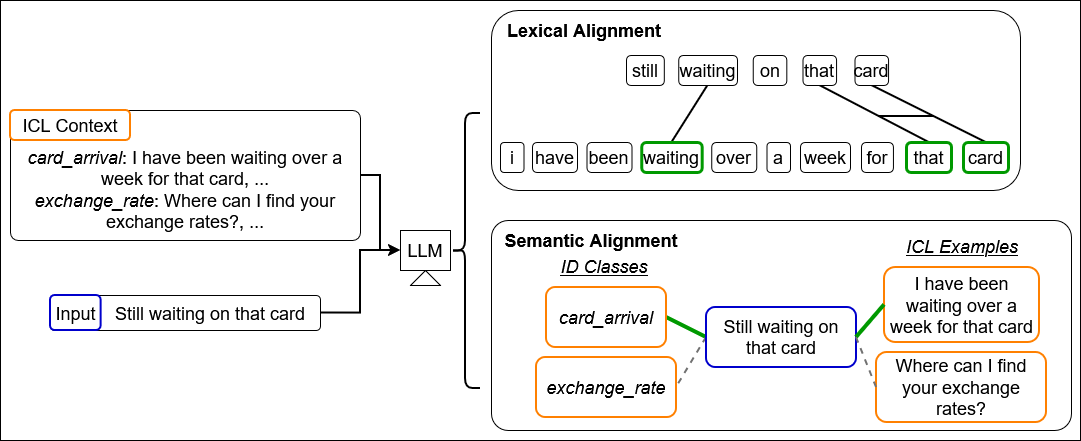
\includegraphics[width=1.\linewidth]{figures/align_examples}
	
	\caption{Examples of lexical and semantic alignment induced in an LLM via ICL prompting. Orange represents the ICL context, blue represents the input, and green represents strong alignment. The input is strongly aligned with the ``card\_arrival'' category and examples but not strongly aligned with the ``exchange\_rate'' cateory and examples. 
	}
	\label{fig:atpo_alignexamples}
\end{figure*}

%The proposed \sys leverages the latent knowledge in LLMs for OOD detection using only text prompts. It solves the prompt-only OOD detection problem by first extracting fine-grained knowledge through \textit{alignment} of the input text with ID classes (category labels) and few-shot examples for those classes provided in the \textit{in-context learning (ICL)} prompt. Second, \sys uses the alignment reasoning to generate a continuous OOD score for a sample. The OOD scores for the ID data are used to calculate a \textit{threshold} for OOD detection instead of performing ($C$+1)-classification.
In \gls{syst}, prompt-only OOD detection is performed by leveraging the latent knowledge in LLMs via text prompts. First, fine-grained knowledge is extracted through \textit{alignment} between the input test utterance and ID classes (i.e. the category labels for included ID classes in each dataset) and associated few-shot examples for each class. This \textit{ICL information} and the test utterance are then used, contextualized by the alignment reasoning, to generate an OOD score for the input. This continuous score is generated for all ID test data which is finally used to calculate a \textit{threshold} for OOD detection.

\subsection{Prompt Context and Alignment}

%%\vspace{2mm}
%%\noindent
%\paragraph{In-Context Learning.} Contextualization of any given input $x$ is provided through few-shot ICL. 
%We randomly select $m$ demonstration examples from each ID class to create a demonstration set as context $\mathcal{C}$. Specifically, using ID training examples and labels $(t_i,y_i)$, we curate $\mathcal{C} = \bigcup_{j=1}^{C} \{(t_i,y_i) | y_i = j\}_{i=1}^{m}$ and provide it to an LLM along with the input. Results across the number of ICL examples $m$ and number of ID classes $C$ are presented in Section \ref{sec:disc}.
\subsubsection{In-Context Learning}
For any given input test utterance $x$, contextualization is formulated as few-shot ICL.
A context $\mathcal{C}$ demonstration set is created by randomly selecting $\nu$ demonstration examples from each ID class. Specifically, ID training examples and labels $(t_i,y_i)$ are used to curate context $\mathcal{C} = \bigcup_{j=1}^{C} \{(t_i,y_i)\ |\ y_i = j\}_{i=1}^{\nu}$ for number of ID classes $C$. The context $\mathcal{C}$ is provided to the LLM along with the input test utterance in a prompt $P$.

% li2025tokalign (align = cosine sim)
% https://d197for5662m48.cloudfront.net/documents/publicationstatus/231698/preprint_pdf/889ad760a1b1d9b655bcee61da7b1ac2.pdf - for some potential math
% el2021xlent (lexical and semantic align defs)
% dyer2013simple (fastalign, word align) - for math
% thompson2020cultural (semantic align - meaning of words/phrases are similar)
% srivastava2025measuring (lexical align review) - for some potential math

%%\noindent
\subsubsection{Alignment} 

%We consider here the alignment between an input $x$ and the ID classes $\mathcal{Y}_{ID} = \{1,2,\dots,C\}$ and examples $\mathcal{C}_t = \bigcup_{j=1}^{C} \{t_i | y_i = j\}_{i=1}^{m}$. Specifically, ``alignment'' in this work refers to the \textit{similarity} between the input and the ID classes and their examples in an established comparison space. In the case of ``lexical alignment'', this similarity space is characterized by the \textit{words} in the input and context. In the case of ``semantic alignment'', this similarity space is characterized by the \textit{meaning} associated with the words and phrases in (or the entirety of) the input and context. Note that we do \textit{not} consider Human-LLM alignment \citep{wang2023aligning, ji2023ai} here which is a different topic.
%
%The LLM $f_{LLM}$ establishes the lexical and semantic similarity spaces in which alignment can be performed using the ID classes $\mathcal{Y}_{ID}$ and ICL examples $\mathcal{C}_t$.
%By using the knowledge and reasoning capabilities inherent to LLMs \citep{kumar2025llm}, the LLM identifies the components defining the similarity spaces in the input $x$ and context $\mathcal{C}$. These spaces enable the measurement of alignment between $x$ and the ID classes $\mathcal{Y}_{ID}$ and ICL examples $\mathcal{C}_t$. 
%
%In previous alignment work, the components defining the lexical and semantic spaces would be defined by the user (e.g., cosine similarity) \citep{dyer2013simple,srivastava2025measuring}. However, as we are limited to only prompts, the lexical and semantic spaces and subsequent alignment must be generated entirely by the LLM through the prompt $\mathcal{P}$. 
%
%We induce lexical and semantic alignment in $f_{LLM}$ between $x$ and $(\mathcal{Y}_{ID},\mathcal{C})$ through the prompted generation of \textit{alignment scores} $\mathcal{A} \sim f_{LLM}(\mathcal{P}(x|\mathcal{Y}_{ID},\mathcal{C}))$ where
%\begin{equation}
%\begin{aligned}
%    \mathcal{A}_1 & \sim f_{LLM}(\mathcal{P}(x|y_1,\mathcal{C}_{t,1})) \\
%    \mathcal{A}_2 & \sim f_{LLM}(\mathcal{P}(x|y_2,\mathcal{C}_{t,2})) \\
%    \dots \\
%    \mathcal{A}_C & \sim f_{LLM}(\mathcal{P}(x|y_C,\mathcal{C}_{t,C})), \\
%\end{aligned}
%\end{equation}
%where $\mathcal{A}_i \in \mathbb{R}$ is the alignment score between $x$ and the class $y_i$ with ICL examples $\mathcal{C}_{t,i} = \{t_k | y_k = i\}_{k=1}^{m}$. $\mathcal{A}$ represents the similarity between $x$ and the ID distribution defined by the lexical and semantic spaces informed by the LLM's knowledge and provided context. These alignment scores subsequently inform OOD detection.
Alignment is defined in this study between an input $x$ and ID classes $\mathcal{Y}_{ID} = \{1,2,\dots,C\}$ and ICL examples $\mathcal{C}_t = \bigcup_{j=1}^{C} \{t_i\ |\ y_i = j\}_{i=1}^{\nu}$. The specific ``alignment'' considered is the \textbf{similarity} between the input and the ID classes and ICL examples in some comparison space. Two comparison spaces are established for this work. First, ``lexical alignment'', is a comparison space characterized by the \textit{words} in the input and the context, i.e. the words comprising the ID classes and in the ICL examples. Second, ``semantic alignment'', is a comparison space characterized by the \textit{meaning} associated with the words and phrases in (or entirety of) the input, the ID classes, and the ICL examples. Semantic alignment measures similarities between the meanings within the input and the meanings present in the context. An example of both types of alignment is shown in \ref{fig:atpo_alignexamples}. Importantly, ``alignment'' here does not refer to Human-LLM alignment \cite{wang2023aligning,ji2023ai} which is an entirely different topic and is not relevant.

An LLM $f_{LLM}$ establishes the lexical and semantic comparison spaces for alignment using the ID classes $\mathcal{Y}_{ID}$ and ICL examples $\mathcal{C}_t$. Through the knowledge and reasoning capabilities inherent to LLMs \cite{kumar2025llm}, the LLM can isolate and extract components in the input $x$ and context $\mathcal{C}$ that define the comparison spaces. These spaces define the measurement basis of alignment between $x$ and the ID classes $\mathcal{Y}_{ID}$ and ICL examples $\mathcal{C}_t$. In previous works on alignment, lexical and semantic spaces would be defined by the user (e.g. cosine similarity) \cite{dyer2013simple,srivastava2025measuring}. Given that prompt-only OOD detection methods are limited to prompts, these definitions are not possible. Instead, the lexical and semantic spaces (as well as subsequent alignment) must be generated entirely through the LLM via prompt $P = \mathcal{P}(\cdot)$ for prompt template $\mathcal{P}$ (see Section \ref{sec:atpo_pinfo} for details). In \gls{syst}, lexical and semantic alignment is induced in $f_{LLM}$ between $x$ and $(\mathcal{Y}_{ID},\mathcal{C})$ through the generation of \textit{alignment scores} $\mathcal{Q} \sim f_{LLM}(\mathcal{P}(x\ |\ \mathcal{Y}_{ID},\mathcal{C}))$ where
\begin{equation}
\begin{aligned}
    \mathcal{Q}_1 & \sim f_{LLM}(\mathcal{P}(x\ |\ y_1,\mathcal{C}_{t,1})) \\
    \mathcal{Q}_2 & \sim f_{LLM}(\mathcal{P}(x\ |\ y_2,\mathcal{C}_{t,2})) \\
    \dots \\
    \mathcal{Q}_C & \sim f_{LLM}(\mathcal{P}(x\ |\ y_C,\mathcal{C}_{t,C})), \\
\end{aligned}
\end{equation}
where any $\mathcal{Q}_i \in \mathbb{R}$ is the alignment score between input test utterance $x$ and the class $y_i$ at $i$. Additionally, $\mathcal{C}_{t,i} = \{t_k\ |\ y_k = i\}_{k=1}^{\nu}$ is the associated ICL examples for class $y_i$.

\subsection{OOD Detection via Thresholding}

%%\vspace{2mm}
%%\noindent
%%\textbf{OOD Scoring.} 
%A function $\mathsf{Parse}(\cdot)$ is used to extract the OOD score $s$ from the generated output of an LLM model $f_{LLM}$
%\begin{equation}
%\begin{split}
%	s & = \mathsf{Parse}(f_{LLM}(\mathcal{P}(x|\mathcal{Y}_{ID},\mathcal{C}))). \\
%\end{split}
%\end{equation}
%The LLM $f_{LLM}$ implicitly utilizes the alignment scores $\mathcal{A}$ during generation to weigh the lexical and semantic similarity between the input $x$ and the ID context $\mathcal{C}$. The alignment informs the extraction of OOD score $s$ by reasoning across the ID classes and ICL examples, as demonstrated in the preceding qualitative study.
%Example outputs $f_{LLM}(\mathcal{P}(x|\mathcal{Y}_{ID},\mathcal{C}))$ are in Section \ref{sec:disc}.
%
%OOD detection is performed by applying a threshold $t_{ID}$ to OOD scores $s$
%\begin{equation}
%  S(s, t_{ID}) =
%  \begin{cases}
%    \text{ID,} & \text{$s \geq t_{ID}$} \\
%    \text{OOD,} & \text{$s < t_{ID}$}. \\
%  \end{cases}
%\end{equation}
%OOD detection performance can be formulated as multiple thresholds over ranked OOD scores (Area Under the Receiver Operating Characteristic curve, AUC) or as a single threshold informed by the statistics of the ID data distribution (95\% False Positive Rate, FPR95) \citep{zhang2023openood}. By leveraging the OOD scores for ID data, OOD detection can be improved through the informed separation of the ID score space and the OOD score space. In particular, near-OOD samples are better detected in this paradigm because uncertain ID samples (which may be similar to near-OOD samples) are considered for the threshold calculation. This is impossible for the previous prompt-only OOD detection method \citep{wang2024beyond} because their direct ($C$+1)-class decision approach \textit{has no notion of OOD scoring}.
%\paragraph{Generation Parsing.} We parse generated outputs to ensure consistency and valid generation of intents and ``unknown''. To prevent false positives from LLM generation of multiple intents or classes (perhaps seen from in-context learning examples), we discard any generated responses containing more than one intent as invalid. Furthermore, to allow for minor variation in generated response, we allow generation up to 7 tokens and check if the number of matched intent tokens is the majority of generated tokens. This handles cases where the ground truth intent is ``card\_payment\_wrong\_exchange\_rate'' but the generated response may be ``incorrect exchange rate for the card payment''.
A function $\mathsf{Parse}(\cdot)$ is used to extract the OOD score $s$ from the generated output of an LLM model $f_{LLM}$
\begin{equation}
\begin{split}
	s & = \mathsf{Parse}(f_{LLM}(\mathcal{P}(x\ |\ \mathcal{Y}_{ID},\mathcal{C}))). \\
\end{split}
\end{equation}
for prompt template $\mathcal{P}$. Specifically, generated outputs are split on a key-phrase ``OOD Score:'' (which was instructed for in the prompt). The most recently generated valid float value generated after the key-phrase was considered as the OOD score.

The alignment scores $\mathcal{Q}$ are used implicitly by $f_{LLM}$ during generation. They assist in quantifying and weighing the lexical and semantic similarity between the input test utterance $x$ and the context $\mathcal{C}$ containing the ID classes and ICL examples. This alignment procedure informs extraction of the OOD score $s$ via reasoning across the ID information.

OOD detection is subsequently performed using OOD scores $s$ by applying a threshold $h_{ID}$
\begin{equation}
  S(s, h_{ID}) =
  \begin{cases}
    \text{ID,} & \text{$s \geq h_{ID}$} \\
    \text{OOD,} & \text{$s < h_{ID}$}. \\
  \end{cases}
\end{equation}
As previously defined in Chapter \ref{diss_bkgd}, metrics for OOD detection rely on some characterization of a threshold and evaluation of the test ID and OOD data against this threshold. To reiterate in the context of prompt-only OOD detection and \gls{syst}, the Area Under the Receiver Operating Characteristic curve (AUC) is an OOD detection metric that uses multiple thresholds over ranked OOD scores. Another OOD detection metric, True Positive Rate at 95\% False Positive Rate (FPR95), uses a single threshold informed by the statistics of the ID data distribution. Leveraging OOD scores for test ID data enables OOD detection through the informed distinction of the ID and OOD score spaces. In particular, and most relevant for this dissertation, near-OOD samples are more effectively detected using ID-informed thresholds because uncertain ID samples (which are very similar to near-OOD samples) are \textit{accounted for in the threshold calculation}. This is impossible for the previous prompt-only OOD detection method \cite{wang2024beyond}. In ($C$+1)-classification, there is \textit{no functionality for OOD scoring}. Thus the ID data distribution cannot be considered during OOD detection.
%$s$ is used for OOD detection of the input $x$ in two ways. First, the continuous range of scores $s \in [0,1]$ allows for a larger metric space for OOD detection compared to the binary decision method proposed in \citet{wang2024beyond}. This establishes OOD detection by considering thresholds across the range of $s$, analogous to the widely-accepted Area Under the Receiver Operating Characteristic curve (AUC) established in OOD detection literature \cite{zhang2023openood}. $s$ may also be used via selecting a single threshold $t_{ID}$
%\begin{equation}
%  S(s, t_{ID}) =
%  \begin{cases}
%    \text{ID,} & \text{$s \geq t_{ID}$} \\
%    \text{OOD,} & \text{$s < t_{ID}$} \\
%  \end{cases}
%\end{equation}
%Both of these approaches are based on the ranking of scores $s$ output from the LLM from ICL and lexical and semantic alignment. They improve upon the previous prompt-only OOD detection method \cite{wang2024beyond}, which used a binary decision for each input $x$, by \textit{quantifying the degree of alignment}. The approach proposed by \citet{wang2024beyond} struggles with detecting samples near the decision boundary as the uncertainty of such ambiguous samples is not accounted for in the detection process. In \sys, the low alignment of such a sample is considered in the detection and provides a clear OOD score metric that establishes \textbf{how much} the input is OOD. This allows subsequent thresholding, whether through AUC or 95\% False Positive Rate \cite{zhang2023openood}, to account for a greater range of possible OOD samples instead of relying only on binary ID and OOD classes.

\subsection{Prompt Instantiation}
\label{sec:atpo_pinfo}

%%\vspace{2mm}
%%\noindent
%%\textbf{Prompt Instantiation.} 
%The ID classes $\mathcal{Y}_{ID}$, ICL context $\mathcal{C}$, and input $x$ are used to instantiate the prompt $P$ from prompt template $\mathcal{P}$, $P = \mathcal{P}(x|\mathcal{Y}_{ID},\mathcal{C})$. Our prompt template $\mathcal{P}$ differs from that of \citet{wang2024beyond} in two ways: 1) we directly encourage alignment between $x$ and ICL context $\mathcal{C}$ for OOD detection, and 2) we do not require the LLM to classify $x$, only provide an OOD score. We share $\mathcal{P}$ and examples in Appendix Section 4.
The prompt $P$ for \gls{syst} is instantiated with ID classes $\mathcal{Y}_{ID}$, ICL context $\mathcal{C}$, and input $x$ through a prompt template $\mathcal{P}$, $P = \mathcal{P}(x\ |\ \mathcal{Y}_{ID},\mathcal{C})$. Crucially, the prompt template proposed in \gls{syst} differs from the previous baseline in that 1) alignment between $x$ and context $\mathcal{C}$ is directly encouraged through lexical and semantic spaces, and 2) LLMs are not required to classify $x$, only provide an OOD score.

\subsection{Prompts}
\label{sec:app-prompts}

The prompt templates used by \gls{syst} are detailed here along with examples. For illustrative purposes, all examples are included with only 1 ICL example per class.

The \gls{syst} template is:
\begin{quote}
You are a language model-based Out-of-Distribution (OOD) detector. Your task is to use your internal reasoning to estimate an OOD score for a given test utterance given some contextual In-Distribution (ID) categories and example utterances.

Here are definitions that will elucidate the concepts relevant to your task:

- ID: The samples, i.e. utterances and categories, that define the data domain you are responsible for. You should be familiar with these categories and are trying to identify if any given test utterance is within the ID categories (using the category topics and ID example utterances to help your decision).

- OOD: Everything that is NOT within the ID data domain. Any sample that does not fall within or align with the ID categories and utterances is OOD.

- Lexical alignment: The concept of similarity between a test utterance and the ID data domain based on LEXICAL factors. This includes similarity concepts such as keyword matching, phrasing similarity, and grammatical/tuple patterns.

- Semantic alignment: The concept of similarity between a test utterance and the ID data domain based on SEMANTIC factors. This includes similarity concepts such as closeness of meanings or themes, conceptual comparisons, and similarity of the presented ideas.

1. Category Matching: For each ID category, estimate how well the utterance aligns with it and its examples. Rank the degree of alignment considering the lexical alignment and semantic alignment.

2. Confidence Estimation: Based on your ranking, assign an OOD score indicating how well the top-ranked category aligns with the test utterance. If the utterance does not align well with the top-ranked category, assign a high OOD score. If it aligns strongly with the top-ranked category, assign a low OOD score.

Now apply these steps to the following input:

In-Distribution categories: \{\}

Example In-Distribution utterances:

\{\}

Test utterance: \{\}

Respond with the following information:

Reasoning: <text with your reasoning> 

OOD Score: <float from 0.0 (confidently in-distribution) to 1.0 (confidently out-of-distribution)>

Response:
\end{quote}
An example is:
\begin{quote}
You are a language model-based Out-of-Distribution (OOD) detector. Your task is to use your internal reasoning to estimate an OOD score for a given test utterance given some contextual In-Distribution (ID) categories and example utterances.

Here are definitions that will elucidate the concepts relevant to your task:

- ID: The samples, i.e. utterances and categories, that define the data domain you are responsible for. You should be familiar with these categories and are trying to identify if any given test utterance is within the ID categories (using the category topics and ID example utterances to help your decision).

- OOD: Everything that is NOT within the ID data domain. Any sample that does not fall within or align with the ID categories and utterances is OOD.

- Lexical alignment: The concept of similarity between a test utterance and the ID data domain based on LEXICAL factors. This includes similarity concepts such as keyword matching, phrasing similarity, and grammatical/tuple patterns.

- Semantic alignment: The concept of similarity between a test utterance and the ID data domain based on SEMANTIC factors. This includes similarity concepts such as closeness of meanings or themes, conceptual comparisons, and similarity of the presented ideas.

1. Category Matching: For each ID category, estimate how well the utterance aligns with it and its examples. Rank the degree of alignment considering the lexical alignment and semantic alignment.

2. Confidence Estimation: Based on your ranking, assign an OOD score indicating how well the top-ranked category aligns with the test utterance. If the utterance does not align well with the top-ranked category, assign a high OOD score. If it aligns strongly with the top-ranked category, assign a low OOD score.

Now apply these steps to the following input:

In-Distribution categories: \textit{card\_arrival, card\_linking, exchange\_rate, card\_payment\_wrong\_exchange\_rate, extra\_charge\_on\_statement}

Example In-Distribution utterances:

\textit{card\_arrival: [Is there a way to track the delivery of my card?], ...}

   \textit{card\_linking: [How do I add an existing card to the app?], ...}
   
   \textit{exchange\_rate: [Where can I find your exchange rates?], ...}
   
   \textit{card\_payment\_wrong\_exchange\_rate: [The exchange rate was incorrect for an item I bought.], ...}
   
   \textit{extra\_charge\_on\_statement: [I have been charged a pound for something that appears on my statement], ...}
   
Test utterance: \textit{How do I locate my card?}

Respond with the following information:

Reasoning: <text with your reasoning> 

OOD Score: <float from 0.0 (confidently in-distribution) to 1.0 (confidently out-of-distribution)>

Response:
\end{quote}

The prompt for \gls{syst} can be modulated in several ways to account for various degrees of induced alignment. In one modulation, denoted as Nonspecified Alignment, alignment is still induced but it is not specified to the LLM that lexical and semantic alignment should be considered.
For \gls{syst}-Nonspecified Alignment, the template is:
\begin{quote}
You are a language model-based Out-of-Distribution (OOD) detector. Your task is to use your internal reasoning to estimate an OOD score for a given test utterance. You will also be provided with the set of In-Distribution (ID) categories and several example utterances from each category as additional context. Use the following structured reasoning steps to estimate an OOD score for a given test utterance:

1. Category Matching: For each ID category, estimate how well the utterance aligns with it and its examples. Use your knowledge of language, context, and category semantics, along with the examples for each category, to rank the degree of alignment.

2. Confidence Estimation: Based on your ranking, assign an OOD score indicating how well the top-ranked category aligns with the test utterance. If the utterance does not align well with the top-ranked category, assign a high OOD score. If it aligns strongly with the top-ranked category, assign a low OOD score.

Now apply these steps to the following input:

In-Distribution categories: \{\}

Example In-Distribution utterances:

\{\}

Test utterance: \{\}

Return an OOD score from 0.0 (confidently in-distribution) to 1.0 (confidently out-of-distribution).

Response:
\end{quote}
Similarly, for \gls{syst} with only reasoning and no specified lexical or semantic alignment (denoted as ``Reasoning''), modulated behavior is induced that continues to leverage alignment-based reasoning over the ID classes and ICL context but not to the depth proposed in \gls{syst}.
For \gls{syst}-Reasoning, the template is:
\begin{quote}
You are a language model-based Out-of-Distribution (OOD) detector. Your task is to use your internal reasoning to estimate an OOD score for a given test utterance. You will also be provided with the set of In-Distribution (ID) categories and several example utterances from each category as additional context. Use the following structured reasoning steps to estimate an OOD score for a given test utterance:

1. Category Matching: For each ID category, estimate how well the utterance aligns with it and its examples. Use your knowledge of language, context, and category semantics, along with the examples for each category, to rank the degree of alignment.

2. Confidence Estimation: Based on your ranking, assign an OOD score indicating how well the top-ranked category aligns with the test utterance. If the utterance does not align well with the top-ranked category, assign a high OOD score. If it aligns strongly with the top-ranked category, assign a low OOD score.

Now apply these steps to the following input:

In-Distribution categories: \{\}

Example In-Distribution utterances:

\{\}

Test utterance: \{\}

Respond with the following information:

Reasoning: <text with your reasoning>

OOD Score: <float from 0.0 (confidently in-distribution) to 1.0 (confidently out-of-distribution)>

Response:
\end{quote}

\section{Experimentation}
\label{sec:propwork-atpo-exp}

\subsection{Qualitative Results for Alignment in LLMs}

%Here we present a brief qualitative study illustrating the ability of the LLM to perform alignment using only prompts. We prompted an LLM, \textbf{Gemma-12B}\footnote{\url{https://huggingface.co/google/gemma-3-12b-it}} \citep{team2025gemma} with the ICL context and a test utterance from the dialogue intent dataset Banking  \citep{casanueva2020efficient}. The provided ID classes were \{\texttt{card\_arrival, card\_linking, exchange\_rate, card\_payment\_wrong\_exchange\_rate, extra\_charge\_on\_statement}\} and an ICL example for class \texttt{card\_arrival} was ``\textit{I have been waiting over a week. Is the card still coming?}". The test input was ``\textit{still waiting on that card}".
%
%Gemma-12B provided the following response when prompted to perform OOD detection using lexical and semantic alignment:
%\begin{quote}
%\texttt{1. Category Matching:}
%
%*   **\texttt{card\_arrival:}** \texttt{This category seems like the best fit. The utterance directly relates to the arrival of a card, which is the core topic of this category. Furthermore, the words "card" and "waiting" appear frequently in the provided category examples. Alignment Score: 0.9}
%
%*   **\texttt{card\_linking:}** \texttt{This category is about linking a card, not waiting for it. While many examples contain the word ``card'', they are generally unrelated. Alignment Score: 0.1} 
%
%*   **\texttt{exchange\_rate:}** \texttt{This category is about currency exchange rates, completely unrelated. Alignment Score: 0.0}
%
%*   **\texttt{card\_payment\_wrong\_exchange\_rate:}** \texttt{This is about incorrect exchange rates on payments, not card arrival. Alignment Score: 0.0}
%
%*   **\texttt{extra\_charge\_on\_statement:}** \texttt{This is about unexpected charges, not card arrival. Alignment Score: 0.0}
%
%\texttt{2. Confidence Estimation:}
%
%\texttt{The utterance "still waiting on that card" aligns strongly with the "card\_arrival" category. The example utterances in this category frequently discuss the delay or non-arrival of a card. The alignment score of 0.9 suggests a high degree of similarity. Therefore, I would assign a low OOD score.}
%
%\texttt{OOD Score: 0.1}
%\end{quote}
%The response from Gemma-12B highlights principled formulations of the lexical and semantic space for alignment. The LLM was able to identify the similarity between the test input $x$ against the provided ID categories $\mathcal{Y}_{ID}$ and ICL examples $\mathcal{C}_t$ using lexical and semantic comparisons. For \textit{lexical alignment}, the LLM identifies the presence of ``card'' and ``waiting'' as matched words in the ICL examples. For \textit{semantic alignment}, the LLM identifies a core topic of the \texttt{card\_arrival} category as ``arrival of a card'' and is able to align the same meaning in the test input to the core semantic topic. The LLM further identifies that the ICL examples for \texttt{card\_arrival} define a semantic space of ``delay'' and ``non-arrival'' for ``cards'', further aligning the test input while eliminating the other categories. The generated alignment scores $\mathcal{A}$ inform the final OOD score $s$ of 0.1.
%
%Note here that the model is generating an OOD score which is higher for inputs considered to be \textit{more OOD}. This is opposite to the traditional OOD scoring scale which considers lower scores to be more OOD. We resolve this by simply taking $1-s$ as the metric for OOD detection (see Section \ref{sec:exp}).
An initial qualitative study is presented to establish the ability of LLMs to perform sophisticated alignment, i.e. via lexical and semantic comparison spaces, using only prompts. An LLM, \textbf{Gemma-12B} (from huggingface: \url{https://huggingface.co/google/gemma-3-12b-it}) \citep{team2025gemma}, was prompted with ID classes, ICL context, and an input test utterance from the dialogue intent dataset  Banking \citep{casanueva2020efficient}. ID classes provided included \{\texttt{card\_arrival, card\_linking, exchange\_rate, card\_payment\_wrong\_exchange\_rate, extra\_charge\_on\_statement}\}. One example ICL example for the \texttt{card\_arrival} class was ``\textit{I have been waiting over a week. Is the card still coming?}". The input test utterance was ``\textit{still waiting on that card}".

The following response was generated by Gemma-12B using the \gls{syst} prompt inducing lexical and semantic alignment:
\begin{quote}
\texttt{1. Category Matching:}

*   **\texttt{card\_arrival:}** \texttt{This category seems like the best fit. The utterance directly relates to the arrival of a card, which is the core topic of this category. Furthermore, the words "card" and "waiting" appear frequently in the provided category examples. Alignment Score: 0.9}

*   **\texttt{card\_linking:}** \texttt{This category is about linking a card, not waiting for it. While many examples contain the word ``card'', they are generally unrelated. Alignment Score: 0.1} 

*   **\texttt{exchange\_rate:}** \texttt{This category is about currency exchange rates, completely unrelated. Alignment Score: 0.0}

*   **\texttt{card\_payment\_wrong\_exchange\_rate:}** \texttt{This is about incorrect exchange rates on payments, not card arrival. Alignment Score: 0.0}

*   **\texttt{extra\_charge\_on\_statement:}** \texttt{This is about unexpected charges, not card arrival. Alignment Score: 0.0}

\texttt{2. Confidence Estimation:}

\texttt{The utterance "still waiting on that card" aligns strongly with the "card\_arrival" category. The example utterances in this category frequently discuss the delay or non-arrival of a card. The alignment score of 0.9 suggests a high degree of similarity. Therefore, I would assign a low OOD score.}

\texttt{OOD Score: 0.1}
\end{quote}
The generated response reveals principled characterization and leveraging of lexical and semantic comparison spaces. The LLM identified lexical and semantic alignment between the input test utterance $x$ and the provided ID classes $\mathcal{Y}_{ID}$ and ICL examples $\mathcal{C}_t$. For \textit{lexical alignment}, the words ``card'' and ``waiting'' were matched between $x$ and examples in $\mathcal{C}_t$. For \textit{semantic alignment}, the core topic of the \texttt{card\_arrival} class, ``arrival of a card'', was identified and aligned with the same meaning present in $x$. Additionally, Gemma-12B identified that ICL examples for \texttt{card\_arrival} established a semantic space of ``delay'' and ``non-arrival'' for ``cards'', simultaneously strengthening the alignment between $x$ and the ID class while eliminating all the other classes. As a final illustrative support for \gls{syst}, Gemma-12B generated alignment scores $\mathcal{Q}$ that informed the final OOD score $s$ of 0.1.

It is important to note that with \gls{syst}, LLMs are generating an \textbf{OOD score} which is higher for inputs considered to be \textit{more OOD}. This is opposite to traditional OOD scoring, which considers lower scores to be more OOD. This is easily adjusted for by simply taking $1-s$ as the values used for computation of OOD detection metrics.

\subsection{Dataset and Experiment Details}
\label{sec:app-exp}

% \subsection{Setup}

The established experimental setup for prompt-only OOD detection was used \cite{wang2024beyond}.

%\begin{table*}[t!]
%%\small
%\centering
%\caption{OOD detection results, Recall and F-Score (F), between \gls{syst}, \gls{syst}-Nonspecified Alignment (\gls{syst}-NA), \gls{syst}-Reasoning (\gls{syst}-R) and the previous prompt-only OOD detection method (POD). Best results are in \textbf{bold}. }
%\vspace{0.1cm}
%\scalebox{0.73}{
%\begin{tabular}{|l|l|cccccccccccccc|}
%\hline
%\multicolumn{2}{|c|}{} & \multicolumn{2}{c}{Banking} & \multicolumn{2}{c}{CLINC} & \multicolumn{2}{c}{Stack} & \multicolumn{2}{c}{20NG} & \multicolumn{2}{c}{Dbpedia} & \multicolumn{2}{c}{Snips} & \multicolumn{2}{|c|}{Avg.} \\ \hline
%\multicolumn{2}{|c|}{} & Recall & F & Recall & F & Recall & F & Recall & F & Recall & F & Recall & F &  \multicolumn{1}{|c}{Recall} & \multicolumn{1}{c|}{F} \\ \hline
%\multirow{4}{*}{Mistral-7B}  &  \textit{POD}        &   43.74 & 52.79  &   69.50 & 70.20  &   39.20 & 48.95  &   12.53 & 13.80  &   0.43 & 19.73  &   2.50 & 43.19  &   \multicolumn{1}{|c}{27.98} & \multicolumn{1}{c|}{41.44}  \\
%                             &  \cellcolor{rowGray} \textit{\gls{syst}-NA} &  \cellcolor{rowGray} 84.75 &  \cellcolor{rowGray} 78.36  & \cellcolor{rowGray}  92.50 &  \cellcolor{rowGray} 88.56 &  \cellcolor{rowGray} 93.87 &  \cellcolor{rowGray} 87.88  & \cellcolor{rowGray}  2.80 &  \cellcolor{rowGray} 22.65  & \cellcolor{rowGray}  80.86 &  \cellcolor{rowGray} 79.56  &  \cellcolor{rowGray} 44.50 &  \cellcolor{rowGray} 64.37 &  \multicolumn{1}{|c}{\cellcolor{rowGray} 66.55} &  \multicolumn{1}{c|}{\cellcolor{rowGray} 70.23} \\ 
%                             &  \cellcolor{rowGray} \textit{\gls{syst}-R} &  \cellcolor{rowGray} 84.75 &  \cellcolor{rowGray} 78.36 & \cellcolor{rowGray}  95.67 &  \cellcolor{rowGray} 87.49 &  \cellcolor{rowGray} 94.93 &  \cellcolor{rowGray} 87.92 & \cellcolor{rowGray}  40.40 &  \cellcolor{rowGray} 48.87 & \cellcolor{rowGray}  86.57 &  \cellcolor{rowGray} 81.43 &  \cellcolor{rowGray} 54.50 &  \cellcolor{rowGray} 64.79 &  \multicolumn{1}{|c}{\cellcolor{rowGray} 76.14} &  \multicolumn{1}{c|}{\cellcolor{rowGray} 74.81}  \\  
%                             &  \cellcolor{rowGray} \textit{\gls{syst}} &  \cellcolor{rowGray} 89.75 &  \cellcolor{rowGray} 80.69 & \cellcolor{rowGray} 99.67 &  \cellcolor{rowGray} 91.57 &  \cellcolor{rowGray} 93.60 &  \cellcolor{rowGray} 85.83 & \cellcolor{rowGray} 48.53 &  \cellcolor{rowGray} 51.45 & \cellcolor{rowGray} 53.29 &  \cellcolor{rowGray} 60.49 &  \cellcolor{rowGray} 87.50 &  \cellcolor{rowGray} 80.64 &  \multicolumn{1}{|c}{\cellcolor{rowGray} \textbf{78.72}} &  \multicolumn{1}{c|}{\cellcolor{rowGray} \textbf{75.11}}  \\  \hline
%\multirow{4}{*}{Qwen-8B}     &  \textit{POD}        &   86.38 & 83.65  &   96.83 & 94.09  &   95.33 & 86.41  &   48.80 & 46.76  &   75.00 & 79.49  &   94.00 & 91.09  &   \multicolumn{1}{|c}{82.72} &   \multicolumn{1}{c|}{80.25} \\
%                             &  \cellcolor{rowGray} \textit{\gls{syst}-NA} &  \cellcolor{rowGray} 92.88 &  \cellcolor{rowGray} 89.22 &  \cellcolor{rowGray} 99.50 &  \cellcolor{rowGray} 96.58 &  \cellcolor{rowGray} 98.40 &  \cellcolor{rowGray} 93.53 & \cellcolor{rowGray}  39.20 &  \cellcolor{rowGray} 51.56 & \cellcolor{rowGray}  90.71 &  \cellcolor{rowGray} 87.65 &  \cellcolor{rowGray} 82.00 &  \cellcolor{rowGray} 83.47 &   \multicolumn{1}{|c}{\cellcolor{rowGray} 83.78} &   \multicolumn{1}{c|}{\cellcolor{rowGray} 83.67} \\ %\hline
%                             &  \cellcolor{rowGray} \textit{\gls{syst}-R} &  \cellcolor{rowGray} 92.88 &  \cellcolor{rowGray} 88.73 &  \cellcolor{rowGray} 99.83 &  \cellcolor{rowGray} 97.21 &  \cellcolor{rowGray} 98.53 &  \cellcolor{rowGray} 93.81 & \cellcolor{rowGray} 38.93 &  \cellcolor{rowGray} 51.27 & \cellcolor{rowGray} 89.00 &  \cellcolor{rowGray} 87.65 &  \cellcolor{rowGray} 78.50 &  \cellcolor{rowGray} 81.39 &   \multicolumn{1}{|c}{\cellcolor{rowGray} 82.95} &   \multicolumn{1}{c|}{\cellcolor{rowGray} 83.34} \\ 
%                             &  \cellcolor{rowGray} \textit{\gls{syst}}  &  \cellcolor{rowGray} 94.88 &  \cellcolor{rowGray} 91.16 & \cellcolor{rowGray} 99.83 &  \cellcolor{rowGray} 97.44 &  \cellcolor{rowGray} 99.47 &  \cellcolor{rowGray} 91.37 & \cellcolor{rowGray} 30.00 &  \cellcolor{rowGray} 45.40 & \cellcolor{rowGray} 93.00 &  \cellcolor{rowGray} 91.13 &  \cellcolor{rowGray} 98.00 &  \cellcolor{rowGray} 85.76 &  \multicolumn{1}{|c}{\cellcolor{rowGray} \textbf{85.86}} &  \multicolumn{1}{c|}{\cellcolor{rowGray} \textbf{83.71}}  \\  \hline
%\multirow{4}{*}{Gemma-12B}   &   \textit{POD}   &   84.00 & 76.22  &   100.00 & 99.37  &   96.93 & 93.44  &   88.67 & 53.15  &   63.57 & 72.63  &   89.50 & 94.82  &   \multicolumn{1}{|c}{87.11} &   \multicolumn{1}{c|}{81.60} \\
%                             &  \cellcolor{rowGray} \textit{\gls{syst}-NA}  &  \cellcolor{rowGray} 96.25 &  \cellcolor{rowGray} 89.03 &  \cellcolor{rowGray} 99.83 &  \cellcolor{rowGray} 94.23 & \cellcolor{rowGray}  98.80 &  \cellcolor{rowGray} 93.62 & \cellcolor{rowGray}  50.93 &  \cellcolor{rowGray} 57.84 &  \cellcolor{rowGray} 97.00 &  \cellcolor{rowGray} 91.03 &  \cellcolor{rowGray} 94.50 &  \cellcolor{rowGray} 83.69 &   \multicolumn{1}{|c}{ \cellcolor{rowGray} 89.55} &   \multicolumn{1}{c|}{ \cellcolor{rowGray} 84.91} \\ %\hline
%                             &  \cellcolor{rowGray} \textit{\gls{syst}-R}  &  \cellcolor{rowGray} 95.63 &  \cellcolor{rowGray} 88.17 &  \cellcolor{rowGray} 99.83 &  \cellcolor{rowGray} 94.70 & \cellcolor{rowGray} 98.80 &  \cellcolor{rowGray} 93.32 & \cellcolor{rowGray} 51.20 &  \cellcolor{rowGray} 57.90 &  \cellcolor{rowGray} 97.29 &  \cellcolor{rowGray} 90.33 &  \cellcolor{rowGray} 94.50 &  \cellcolor{rowGray} 84.69 &   \multicolumn{1}{|c}{ \cellcolor{rowGray} 89.54} &   \multicolumn{1}{c|}{ \cellcolor{rowGray} 84.85} \\
%                             &  \cellcolor{rowGray} \textit{\gls{syst}}  &  \cellcolor{rowGray} 97.00 &  \cellcolor{rowGray} 90.05 & \cellcolor{rowGray} 100.00 &  \cellcolor{rowGray} 97.64 &  \cellcolor{rowGray} 99.47 &  \cellcolor{rowGray} 90.58 & \cellcolor{rowGray} 57.60 &  \cellcolor{rowGray} 60.10 & \cellcolor{rowGray} 95.14 &  \cellcolor{rowGray} 91.27 &  \cellcolor{rowGray} 96.50 &  \cellcolor{rowGray} 82.83 &  \multicolumn{1}{|c}{\cellcolor{rowGray} \textbf{90.95}} &  \multicolumn{1}{c|}{\cellcolor{rowGray} \textbf{85.41}}  \\  \hline
%\multirow{4}{*}{Deepseek-32B}   &  \textit{POD}        &   47.25 & 50.08  &   57.67 & 58.17  &   51.20 & 52.50  &   41.33 & 37.49  &   54.86 & 56.22  & 46.50 & 62.19 &   \multicolumn{1}{|c}{49.80} &   \multicolumn{1}{c|}{52.77} \\
%                             &  \cellcolor{rowGray} \textit{\gls{syst}-NA}  &  \cellcolor{rowGray} 94.13 &  \cellcolor{rowGray} 90.36 &  \cellcolor{rowGray} 100.00 &  \cellcolor{rowGray} 98.30 &  \cellcolor{rowGray} 98.40 &  \cellcolor{rowGray} 93.38  &  \cellcolor{rowGray} 59.87 &  \cellcolor{rowGray} 64.95  &  \cellcolor{rowGray} 84.14 &  \cellcolor{rowGray} 84.91  &  \cellcolor{rowGray} 96.50 &  \cellcolor{rowGray} 89.82  &   \multicolumn{1}{|c}{\cellcolor{rowGray} 88.84} &   \multicolumn{1}{c|}{\cellcolor{rowGray} 86.95} \\ %\hline
%                             &  \cellcolor{rowGray} \textit{\gls{syst}-R}  &  \cellcolor{rowGray} 92.88 &  \cellcolor{rowGray} 89.22  &  \cellcolor{rowGray} 99.67 &  \cellcolor{rowGray} 98.10  &  \cellcolor{rowGray} 98.00 &  \cellcolor{rowGray} 92.70 &  \cellcolor{rowGray} 55.73 &  \cellcolor{rowGray} 61.36 &  \cellcolor{rowGray} 100.00 &  \cellcolor{rowGray} 90.54 &  \cellcolor{rowGray} 93.75 &  \cellcolor{rowGray} 87.45 &   \multicolumn{1}{|c}{\cellcolor{rowGray} 90.00} &   \multicolumn{1}{c|}{\cellcolor{rowGray} 86.56} \\
%                             &  \cellcolor{rowGray} \textit{\gls{syst}}  &  \cellcolor{rowGray} 95.63 &  \cellcolor{rowGray} 90.97 & \cellcolor{rowGray} 100.00 &  \cellcolor{rowGray} 97.64 &  \cellcolor{rowGray} 99.07 &  \cellcolor{rowGray} 90.03 & \cellcolor{rowGray} 74.93 &  \cellcolor{rowGray} 71.08 & \cellcolor{rowGray} 87.14 &  \cellcolor{rowGray} 87.90 &  \cellcolor{rowGray} 97.50 &  \cellcolor{rowGray} 87.04 &  \multicolumn{1}{|c}{\cellcolor{rowGray} \textbf{92.38}} &  \multicolumn{1}{c|}{\cellcolor{rowGray} \textbf{87.44}}  \\  \hline
%\end{tabular}
%}
%\label{tab:atpo_results_promptonly}
%\end{table*}

\begin{table*}[t]
%\small
\centering
\caption{Information for datasets used in \syst experimentation.}
\vspace{0.1cm}
\scalebox{1.}{
\begin{tabular}{|l|c|c|c|c|c|c|}
\hline
 & CLINC & Banking & Stack & 20NG & Dbpedia & Snips \\ \hline
Avg. Utterance Length & 9 & 12 & 50 & 100 & 100 & 49 \\ \hline
\# Classes &  150 &  77 & 20 & 20 & 14 & 7 \\ \hline
Train Set Size &  15000 &  9003 & 2000 & 2599 & 660 & 9830 \\ \hline
- Samples per Class &  100 & / & 100 & / & / & / \\ \hline
Test Set Size &  5500 &  3080 & 1000 & 5604 & 628 & 200 \\ \hline
- Samples per Class &  30 &  / & 50 & / & / & 100 \\ \hline
\end{tabular}
}
\label{tab:atpo_dsetinfo}
\end{table*}

\subsubsection{Datasets}
The Banking, CLINC, StackOverflow, 20NewsGroups, Dbpedia, and Snips datasets were used for experimental evaluation. Details for each dataset are provided here and in \ref{tab:atpo_dsetinfo}:
\begin{itemize}
    \item Banking77 (\textbf{Banking}) \citep{casanueva2020efficient}, - An intent dataset with fine-grained intent classes related to banking topics. It consists of 77 intent classes. 5 classes were used as the ID dataset and 20 distinct classes as the OOD dataset.
    \item CLINC150 (\textbf{CLINC}) \citep{larson2019evaluation}, - An intent dataset designed for OOD detection. It consists of 150 intent classes. 5 classes were used as the ID dataset and 20 distinct classes as the OOD dataset.
    \item StackOverflow (\textbf{Stack}) \citep{xu2015short} - An intent dataset with various intent classes from the StackOverflow website. It contains 20 intent classes. 5 classes were used as the ID dataset and the remaining 15 classes as the OOD dataset. Additionally, only 100 samples were taken per class for the training dataset and 50 samples per class for the testing dataset.
    \item 20NewsGroups (\textbf{20NG}) \citep{lang1995newsweeder} - A text classification dataset. It contains 20 classes with labels related to various topics in a news setting. 5 classes were used as the ID dataset and the remaining 15 classes as the OOD dataset. Additionally, only 100 samples were taken per class for the training dataset and 50 samples per class for the testing dataset. Furthermore, inputs were truncated to 100 characters (from an original average utterance length of 1950) in order to allow models and inputs to fit in memory on available computation resources. This was empirically verified to be sufficient in capturing class-relevant information in the input.
    \item \textbf{Dbpedia} \citep{lehmann2015dbpedia} - A text classification dataset containing facts extracted from Wikipedia. The 14-class version from previous text OOD detection works \citep{arora2021types} was used. 5 classes were used as the ID dataset and the remaining 9 classes as the OOD dataset. Similar to 20NG, inputs were truncated to 100 characters (from the original average utterance length of 293) in order to allow models and inputs to fit in memory on available computation resources. This was empirically verified to be sufficient in capturing class-relevant information in the input.
    \item \textbf{Snips} \citep{coucke2018snips} - An intent dataset collected from an automatic speech recognition platform. It contains 7 classes. 5 classes were used as the ID dataset and the remaining 2 classes as the OOD dataset.
\end{itemize}

\subsubsection{Models}
Four LLMs were used in experimental evaluations. The first was an instruction-tuned version of Mistral-7B \cite{jiang2023mistral7b} (sourced from huggingface after agreeing to the license: \url{https://huggingface.co/mistralai/Mistral-7B-Instruct-v0.3}). Mistral-7B is a 7.25 billion (B) parameter LLM. The second was Qwen-8B \cite{qwen3technicalreport} (sourced from huggingface: \url{https://huggingface.co/Qwen/Qwen3-8B}). Qwen-8B is a 8.19 B parameter LLM. The third was an instruction-tuned version of Gemma-12B \cite{team2025gemma} (sourced from huggingface after agreeing to the license: \url{https://huggingface.co/google/gemma-3-12b-it}). Gemma-12B is a 12.2 B parameter LLM. The fourth was a version of Deepseek-R1-32B distilled from Qwen \cite{guo2025deepseek} (sourced from huggingface: \url{https://huggingface.co/deepseek-ai/DeepSeek-R1-Distill-Qwen-32B}). Deepseek-R1-Distill-Qwen-32B (or simply Deepseek-32B) is a 32.8 B parameter LLM. Each experimental trial took approximately 1 hour on a single NVIDIA RTX A6000 GPU (for Mistral-7B, Qwen-8B, and Gemma-12B) or four NVIDIA RTX A6000 GPUs (for Deepseek-32B). Use of these models (and all used resources) falls in line with the the research- and ethical-intent of the respective resources. Sampling parameters for \gls{syst} are listed below:
\begin{itemize}
    \item Temperature = 0.01
    \item topP = 0.92
    \item topK = 0
    \item Max Output Tokens = 1000
\end{itemize}
All results presented are from a single run, as the low temperature induced near-deterministic LLM generation. For baselines, the best reported hyperparameters are used (if applicable). Average token throughput per \gls{syst} prompt was 3100.

%\paragraph{Baselines.} \sys is compared against the only previous prompt-only baseline \citep{wang2024beyond} (we name it \textbf{POD}) and latest feature- and logits-based OOD detection methods as representative upper-bounds \citep{baran2023classical,zhang2023openood}: \textbf{CED} \citep{lee2024ced}, which uses auxiliary feature samples to identify OOD samples (we use their KNN version which showed best overall performance),  %experiments with out-of-the-box 
%\textbf{KNN} \citep{sun2022out,uppaal2023fine},  \textbf{MD} \citep{lee2018simple,ren2021simple,uppaal2023fine}, \textbf{ViM} \citep{wang2022vim}, and \textbf{MaxLogit} \citep{hendrycks2019scaling}. \textit{CED failed to converge with Gemma-12B or Deepseek-32B and is not included.} %We were unable to run the classic OOD detection methods for Deepseek-32B and Llama-70B on our available resources. % {\color{red}try Qwen w/out reasoning, try and debug vod-vim if possible (no math?)}\alex{Qwen w/out reasoning is better for VIM but worse for the other two, overall it is still ok though}
\subsubsection{Baselines}
Comparisons with \gls{syst} are made against 1) the only previous prompt-only baseline \cite{wang2024beyond} (denoted henceforth in the experimentation and discussion as ``\textbf{POD}''), and 2) state-of-the-art feature- and logits-based OOD detection methods, included primarily as representative upper-bounds as they have an advantage over prompt-only methods \cite{baran2023classical,zhang2023openood}. Included feature- and logits-based OOD detection methods include: \textbf{CED} \cite{lee2024ced} (uses auxiliary sample features to identify OOD samples, the version used here is their KNN implementation which demonstrated best performance), \textbf{KNN} \cite{sun2022out,uppaal2023fine}, \textbf{MD} \cite{lee2018simple,ren2021simple,uppaal2023fine}, \textbf{ViM} \cite{wang2022vim}, and \textbf{MaxLogit} \cite{hendrycks2019scaling}. Results for CED using Gemma-12B and Deepseek-32B are unavailable because the algorithm failed to converge on those models.

%\textbf{Evaluation metrics.} We use the standard %Area Under the Receiver Operating Characteristic curve (\textbf{AUC}) 
%\textbf{AUC} as the OOD detection evaluation metric 
%%{\color{blue}when comparing to feature- and logits-based methods} 
%\citep{zhang2023openood}. For POD, we follow its evaluation protocol and use Recall and F-Score over binary ID and OOD classification as the OOD detection metric \citep{wang2024beyond}. We cannot use AUC as POD only does ($C$+1) classification (ID or OOD) \textbf{with no scores}. For \sys, which outputs an OOD score, we use a threshold above which the output is considered ID and below which is considered OOD. We selected the threshold by following OOD detection standard practice, that is of determining the OOD score above which 95\% of the ID samples would be correctly classified as ID (FPR95) \citep{zhang2023openood}. We did not optimize this threshold. 
\gls{syst} and all other baselines are evaluated in their appropriate settings. That is, for traditional OOD detection methods and \gls{syst} (i.e. methods that output a score), AUC is used as the OOD detection metric. However, for POD, the evaluation protocol defined in the previous baseline is used, and use Recall and F-Score over binary $(ID,OOD)$ classification are presented as the OOD detection metric \cite{wang2024beyond}. AUC is undefined with POD as POD only performs ($C$+1)-classification with no scores. \gls{syst} is adapted to this evaluation setting by thresholding the output score, above which an output is considered ``ID'' and below which is considered ``OOD''. The threshold selected follows the OOD detection standard practice of the value above which 95\% of ID samples would be correctly classified as ID (i.e. from the FPR95 OOD detection metric) \cite{zhang2023openood}.

\subsection{Results}
\label{sec:atpo_results}

\begin{table*}[t!]
%\small
\centering
\caption{OOD detection results, Recall, between \syst, \syst-Nonspecified Alignment (\syst-NA), \syst-Reasoning (\syst-R) and the previous prompt-only OOD detection method (POD). %Best results are in \textbf{bold}. 
}
\vspace{0.1cm}
\scalebox{0.85}{
\begin{tabular}{|l|l|ccccccc|}
\hline
\multicolumn{2}{|c|}{} & \multicolumn{1}{c}{Banking} & \multicolumn{1}{c}{CLINC} & \multicolumn{1}{c}{Stack} & \multicolumn{1}{c}{20NG} & \multicolumn{1}{c}{Dbpedia} & \multicolumn{1}{c}{Snips} & \multicolumn{1}{|c|}{Avg.} \\ \hline
\multirow{4}{*}{Mistral-7B}  &  \textit{POD}        &   43.74 &  69.50 &   39.20 &  12.53 &  0.43 &  2.50 &  \multicolumn{1}{|c|}{27.98}  \\
                             &  \cellcolor{rowGray} \textit{\gls{syst}-NA} &  \cellcolor{rowGray} 84.75 &   \cellcolor{rowGray}  92.50 &  \cellcolor{rowGray} 93.87 &   \cellcolor{rowGray}  2.80 &  \cellcolor{rowGray}  80.86 &   \cellcolor{rowGray} 44.50 &  \multicolumn{1}{|c|}{\cellcolor{rowGray} 66.55}  \\ 
                             &  \cellcolor{rowGray} \textit{\gls{syst}-R} &  \cellcolor{rowGray} 84.75 &  \cellcolor{rowGray}  95.67 &   \cellcolor{rowGray} 94.93 &  \cellcolor{rowGray}  40.40 &   \cellcolor{rowGray}  86.57 &    \cellcolor{rowGray} 54.50 &    \multicolumn{1}{|c|}{\cellcolor{rowGray} 76.14}  \\  
                             &  \cellcolor{rowGray} \textit{\gls{syst}} &  \cellcolor{rowGray} 89.75 &  \cellcolor{rowGray} 99.67 &   \cellcolor{rowGray} 93.60 &  \cellcolor{rowGray} 48.53 &  \cellcolor{rowGray} 53.29 &  \cellcolor{rowGray} 87.50 &  \multicolumn{1}{|c|}{\cellcolor{rowGray} \textbf{78.72}}   \\  \hline
\multirow{4}{*}{Qwen-8B}     &  \textit{POD}        &   86.38 &   96.83 &  95.33 & 48.80 & 75.00 &    94.00 &   \multicolumn{1}{|c|}{82.72}  \\
                             &  \cellcolor{rowGray} \textit{\gls{syst}-NA} &  \cellcolor{rowGray} 92.88 &   \cellcolor{rowGray} 99.50 &    \cellcolor{rowGray} 98.40 &   \cellcolor{rowGray}  39.20 &  \cellcolor{rowGray}  90.71 &   \cellcolor{rowGray} 82.00 &    \multicolumn{1}{|c|}{\cellcolor{rowGray} 83.78}\\ %\hline
                             &  \cellcolor{rowGray} \textit{\gls{syst}-R} &  \cellcolor{rowGray} 92.88 &   \cellcolor{rowGray} 99.83 &   \cellcolor{rowGray} 98.53 &   \cellcolor{rowGray} 38.93 &   \cellcolor{rowGray} 89.00 &    \cellcolor{rowGray} 78.50 &    \multicolumn{1}{|c|}{\cellcolor{rowGray} 82.95} \\ 
                             &  \cellcolor{rowGray} \textit{\gls{syst}}  &  \cellcolor{rowGray} 94.88 & \cellcolor{rowGray} 99.83 &  \cellcolor{rowGray} 99.47 &\cellcolor{rowGray} 30.00 &  \cellcolor{rowGray} 93.00 &  \cellcolor{rowGray} 98.00 &    \multicolumn{1}{|c|}{\cellcolor{rowGray} \textbf{85.86}}   \\  \hline
\multirow{4}{*}{Gemma-12B}   &   \textit{POD}   &   84.00 &    100.00 & 96.93 &   88.67 &  63.57 &   89.50 &    \multicolumn{1}{|c|}{87.11}  \\
                             &  \cellcolor{rowGray} \textit{\gls{syst}-NA}  &  \cellcolor{rowGray} 96.25 &   \cellcolor{rowGray} 99.83 &  \cellcolor{rowGray}  98.80 &   \cellcolor{rowGray}  50.93 &   \cellcolor{rowGray} 97.00 &   \cellcolor{rowGray} 94.50 &     \multicolumn{1}{|c|}{ \cellcolor{rowGray} 89.55}\\ %\hline
                             &  \cellcolor{rowGray} \textit{\gls{syst}-R}  &  \cellcolor{rowGray} 95.63 &   \cellcolor{rowGray} 99.83 &  \cellcolor{rowGray} 98.80 & \cellcolor{rowGray} 51.20 &  \cellcolor{rowGray} 97.29 &   \cellcolor{rowGray} 94.50 &   \multicolumn{1}{|c|}{ \cellcolor{rowGray} 89.54}  \\
                             &  \cellcolor{rowGray} \textit{\gls{syst}}  &  \cellcolor{rowGray} 97.00 &  \cellcolor{rowGray} 100.00 &   \cellcolor{rowGray} 99.47 &  \cellcolor{rowGray} 57.60 &  \cellcolor{rowGray} 95.14 &   \cellcolor{rowGray} 96.50 &  \multicolumn{1}{|c|}{\cellcolor{rowGray} \textbf{90.95}}  \\  \hline
\multirow{4}{*}{Deepseek-32B}   &  \textit{POD}        &   47.25 &  57.67 &  51.20 &  41.33 &   54.86 & 46.50 & \multicolumn{1}{|c|}{49.80}\\
                             &  \cellcolor{rowGray} \textit{\gls{syst}-NA}  &  \cellcolor{rowGray} 94.13 &    \cellcolor{rowGray} 100.00 &  \cellcolor{rowGray} 98.40 &   \cellcolor{rowGray} 59.87 &   \cellcolor{rowGray} 84.14 &  \cellcolor{rowGray} 96.50 &    \multicolumn{1}{|c|}{\cellcolor{rowGray} 88.84} \\ %\hline
                             &  \cellcolor{rowGray} \textit{\gls{syst}-R}  &  \cellcolor{rowGray} 92.88 &  \cellcolor{rowGray} 99.67 &    \cellcolor{rowGray} 98.00 &  \cellcolor{rowGray} 55.73 &  \cellcolor{rowGray} 100.00 &   \cellcolor{rowGray} 93.75 &  \multicolumn{1}{|c|}{\cellcolor{rowGray} 90.00}  \\
                             &  \cellcolor{rowGray} \textit{\gls{syst}}  &  \cellcolor{rowGray} 95.63 &  \cellcolor{rowGray} 100.00 &    \cellcolor{rowGray} 99.07 &  \cellcolor{rowGray} 74.93 &  \cellcolor{rowGray} 87.14 &   \cellcolor{rowGray} 97.50 &  \multicolumn{1}{|c|}{\cellcolor{rowGray} \textbf{92.38}}  \\  \hline
\end{tabular}
}
\label{tab:atpo_results_promptonly}
\end{table*}

\begin{table*}[t!]
%\small
\centering
\caption{OOD detection results, F-Score (F), between \syst, \syst-Nonspecified Alignment (\syst-NA), \syst-Reasoning (\syst-R) and the previous prompt-only OOD detection method (POD). %Best results are in \textbf{bold}. 
}
\vspace{0.1cm}
\scalebox{0.85}{
\begin{tabular}{|l|l|ccccccc|}
\hline
\multicolumn{2}{|c|}{} & \multicolumn{1}{c}{Banking} & \multicolumn{1}{c}{CLINC} & \multicolumn{1}{c}{Stack} & \multicolumn{1}{c}{20NG} & \multicolumn{1}{c}{Dbpedia} & \multicolumn{1}{c}{Snips} & \multicolumn{1}{|c|}{Avg.} \\ \hline
\multirow{4}{*}{Mistral-7B}  &  \textit{POD}        &   52.79  &  70.20  &   48.95  &    13.80  &  19.73  &    43.19  & \multicolumn{1}{|c|}{41.44}  \\
                             &  \cellcolor{rowGray} \textit{\gls{syst}-NA} &    \cellcolor{rowGray} 78.36  &   \cellcolor{rowGray} 88.56 &    \cellcolor{rowGray} 87.88  &   \cellcolor{rowGray} 22.65  &   \cellcolor{rowGray} 79.56  &   \cellcolor{rowGray} 64.37 &   \multicolumn{1}{|c|}{\cellcolor{rowGray} 70.23} \\ 
                             &  \cellcolor{rowGray} \textit{\gls{syst}-R} &   \cellcolor{rowGray} 78.36 &   \cellcolor{rowGray} 87.49 &  \cellcolor{rowGray} 87.92 &   \cellcolor{rowGray} 48.87 &   \cellcolor{rowGray} 81.43 &    \cellcolor{rowGray} 64.79 &    \multicolumn{1}{|c|}{\cellcolor{rowGray} 74.81}  \\  
                             &  \cellcolor{rowGray} \textit{\gls{syst}} &   \cellcolor{rowGray} 80.69 &  \cellcolor{rowGray} 91.57 &  \cellcolor{rowGray} 85.83 &  \cellcolor{rowGray} 51.45 &  \cellcolor{rowGray} 60.49 &  \cellcolor{rowGray} 80.64 &    \multicolumn{1}{|c|}{\cellcolor{rowGray} \textbf{75.11}}  \\  \hline
\multirow{4}{*}{Qwen-8B}     &  \textit{POD}        &    83.65  &  94.09  &   86.41  &  46.76  &   79.49  &  91.09  &    \multicolumn{1}{|c|}{80.25} \\
                             &  \cellcolor{rowGray} \textit{\gls{syst}-NA} &   \cellcolor{rowGray} 89.22 &   \cellcolor{rowGray} 96.58 &  \cellcolor{rowGray} 93.53 &   \cellcolor{rowGray} 51.56 &  \cellcolor{rowGray} 87.65 &   \cellcolor{rowGray} 83.47 &    \multicolumn{1}{|c|}{\cellcolor{rowGray} 83.67} \\ %\hline
                             &  \cellcolor{rowGray} \textit{\gls{syst}-R} &  \cellcolor{rowGray} 88.73 &   \cellcolor{rowGray} 97.21 &   \cellcolor{rowGray} 93.81 &  \cellcolor{rowGray} 51.27 &  \cellcolor{rowGray} 87.65 &  \cellcolor{rowGray} 81.39 &      \multicolumn{1}{|c|}{\cellcolor{rowGray} 83.34} \\ 
                             &  \cellcolor{rowGray} \textit{\gls{syst}}  &  \cellcolor{rowGray} 91.16 &  \cellcolor{rowGray} 97.44 &   \cellcolor{rowGray} 91.37 & \cellcolor{rowGray} 45.40 &  \cellcolor{rowGray} 91.13 &   \cellcolor{rowGray} 85.76 &    \multicolumn{1}{|c|}{\cellcolor{rowGray} \textbf{83.71}}  \\  \hline
\multirow{4}{*}{Gemma-12B}   &   \textit{POD}   &   76.22  &    99.37  &   93.44  &    53.15  &   72.63  &   94.82  &    \multicolumn{1}{|c|}{81.60} \\
                             &  \cellcolor{rowGray} \textit{\gls{syst}-NA}  &   \cellcolor{rowGray} 89.03 &    \cellcolor{rowGray} 94.23 &  \cellcolor{rowGray} 93.62 &  \cellcolor{rowGray} 57.84 &    \cellcolor{rowGray} 91.03 &  \cellcolor{rowGray} 83.69 &    \multicolumn{1}{|c|}{ \cellcolor{rowGray} 84.91} \\ %\hline
                             &  \cellcolor{rowGray} \textit{\gls{syst}-R}  &   \cellcolor{rowGray} 88.17 &   \cellcolor{rowGray} 94.70 &  \cellcolor{rowGray} 93.32 &  \cellcolor{rowGray} 57.90 &   \cellcolor{rowGray} 90.33 &   \cellcolor{rowGray} 84.69 &    \multicolumn{1}{|c|}{ \cellcolor{rowGray} 84.85} \\
                             &  \cellcolor{rowGray} \textit{\gls{syst}}  &   \cellcolor{rowGray} 90.05 &  \cellcolor{rowGray} 97.64 &   \cellcolor{rowGray} 90.58 & \cellcolor{rowGray} 60.10 &  \cellcolor{rowGray} 91.27 &   \cellcolor{rowGray} 82.83 &   \multicolumn{1}{|c|}{\cellcolor{rowGray} \textbf{85.41}}  \\  \hline
\multirow{4}{*}{Deepseek-32B}   &  \textit{POD}        &   50.08  &   58.17  &    52.50  &   37.49  &    56.22  &  62.19 &   \multicolumn{1}{|c|}{52.77} \\
                             &  \cellcolor{rowGray} \textit{\gls{syst}-NA}  &    \cellcolor{rowGray} 90.36 &   \cellcolor{rowGray} 98.30 &    \cellcolor{rowGray} 93.38  &    \cellcolor{rowGray} 64.95  &   \cellcolor{rowGray} 84.91  &   \cellcolor{rowGray} 89.82  &    \multicolumn{1}{|c|}{\cellcolor{rowGray} 86.95} \\ %\hline
                             &  \cellcolor{rowGray} \textit{\gls{syst}-R}  &   \cellcolor{rowGray} 89.22  &   \cellcolor{rowGray} 98.10  &   \cellcolor{rowGray} 92.70 &   \cellcolor{rowGray} 61.36 &   \cellcolor{rowGray} 90.54 &   \cellcolor{rowGray} 87.45 &   \multicolumn{1}{|c|}{\cellcolor{rowGray} 86.56} \\
                             &  \cellcolor{rowGray} \textit{\gls{syst}}  &   \cellcolor{rowGray} 90.97 & \cellcolor{rowGray} 97.64 &   \cellcolor{rowGray} 90.03 &  \cellcolor{rowGray} 71.08 & \cellcolor{rowGray} 87.90 &  \cellcolor{rowGray} 87.04 &    \multicolumn{1}{|c|}{\cellcolor{rowGray} \textbf{87.44}}  \\  \hline
\end{tabular}
}
\label{tab:atpo_results_promptonly_f}
\end{table*}

\begin{table*}[t!]
%\begin{table}[t!]
%\small
\centering
\caption{OOD detection results (AUC) between \syst prompt-only method (\textit{italicized}) and classic feature- and logits-based methods. %Best results are in \textbf{bold}. 
The \textbf{KNN} and \textbf{MD} methods in the table are from a previous feature-based LLM baseline \citep{uppaal2023fine}.  %, best prompt-only results are \underline{underlined}. 
}
\vspace{0.1cm}
\scalebox{0.9}{
\begin{tabular}{|c|l|ccccccc|}
\hline
\multicolumn{2}{|c|}{} & Banking & CLINC & Stack & 20NG & Dbpedia & Snips & \multicolumn{1}{|c|}{Avg.} \\ \hline
%\multirow{8}{*}{\begin{tabular}[c]{@{}c@{}}Mistral-\\7B\end{tabular}}  &  CED                    &   90.55  &   97.71  &   99.60  &   71.35  &   69.79  &   61.57  &   \multicolumn{1}{|c|}{81.76}  \\
\multirow{8}{*}{Mistral-7B}  &  CED                    &   90.55  &   97.71  &   99.60  &   71.35  &   69.79  &   61.57  &   \multicolumn{1}{|c|}{81.76}  \\
                             &  MaxLogit                    &   86.10  &   37.69  &   70.33  &   53.22  &   62.35  &   47.05  &   \multicolumn{1}{|c|}{59.46}  \\ 
                             &  KNN                    &   96.70  &   98.80  &   92.85  &   58.04  &   72.27  &   98.03  &   \multicolumn{1}{|c|}{86.12}  \\ 
                             &  MD                  &   96.48  &   98.84  &   92.95  &   60.01  &   74.84  &   95.95  &   \multicolumn{1}{|c|}{\textbf{86.51}}  \\ 
                             &  ViM                    &   95.89  &   95.57  &   93.08  &   53.85  &   75.21  &   95.11  &   \multicolumn{1}{|c|}{84.79}  \\ \cdashline{2-9}
   &  \cellcolor{rowGray} \textit{\gls{syst}-NA}  &  \cellcolor{rowGray} 86.03  & \cellcolor{rowGray}  96.00  &  \cellcolor{rowGray} 89.42  & \cellcolor{rowGray}  50.88  & \cellcolor{rowGray}  90.18  &  \cellcolor{rowGray} 76.60  &  \multicolumn{1}{|c|}{\cellcolor{rowGray} 81.52}  \\  %\hline
   &  \cellcolor{rowGray} \textit{\gls{syst}-R}  &  \cellcolor{rowGray} 87.14  & \cellcolor{rowGray}  86.28  &  \cellcolor{rowGray} 85.21  & \cellcolor{rowGray}  53.95  & \cellcolor{rowGray}  76.74  &  \cellcolor{rowGray} 76.68  &  \multicolumn{1}{|c|}{\cellcolor{rowGray} 77.67}  \\  
   &  \cellcolor{rowGray} \textit{\gls{syst}}  &  \cellcolor{rowGray} 92.14  & \cellcolor{rowGray}  94.97  &  \cellcolor{rowGray} 93.87  & \cellcolor{rowGray} 65.01  & \cellcolor{rowGray} 89.36  &  \cellcolor{rowGray} 82.09  &  \multicolumn{1}{|c|}{\cellcolor{rowGray} 86.24}  \\  \hline
%\multirow{8}{*}{\begin{tabular}[c]{@{}c@{}}Qwen-\\8B\end{tabular}}     &  CED                    &   82.03  &   42.58  &   63.12  &   97.65  &   71.95  &   62.62  &   \multicolumn{1}{|c|}{69.99}  \\
\multirow{8}{*}{Qwen-8B}     &  CED                    &   82.03  &   42.58  &   63.12  &   97.65  &   71.95  &   62.62  &   \multicolumn{1}{|c|}{69.99}  \\
                             &  MaxLogit                    &   46.24  &   32.02  &   40.36  &   58.57  &   68.13  &   38.74  &   \multicolumn{1}{|c|}{47.34}  \\ 
                             &  KNN                    &   90.90  &   97.65  &   77.57  &   52.56  &   66.26  &   92.85  &   \multicolumn{1}{|c|}{79.63}  \\ 
                             &  MD                     &   94.88  &   98.86  &   85.31  &   51.87  &   77.22  &   95.25  &   \multicolumn{1}{|c|}{83.89}  \\ 
                             &  ViM                    &   94.12  &   98.14  &   86.50  &   53.93  &   73.85  &   94.59  &   \multicolumn{1}{|c|}{83.52}  \\ \cdashline{2-9}
                             &  \cellcolor{rowGray} \textit{\gls{syst}-NA}  &  \cellcolor{rowGray} 91.95  &  \cellcolor{rowGray} 96.20  &  \cellcolor{rowGray} 92.79  & \cellcolor{rowGray}  67.13  & \cellcolor{rowGray}  88.46  &  \cellcolor{rowGray} 91.09  &   \multicolumn{1}{|c|}{\cellcolor{rowGray} 87.94}  \\ %\hline
                             &  \cellcolor{rowGray} \textit{\gls{syst}-R}  &  \cellcolor{rowGray} 95.73  &  \cellcolor{rowGray} 98.60  &  \cellcolor{rowGray} 96.34  & \cellcolor{rowGray}  75.73  & \cellcolor{rowGray}  93.02  &  \cellcolor{rowGray} 87.02  &   \multicolumn{1}{|c|}{\cellcolor{rowGray} 91.07}  \\ 
                            &  \cellcolor{rowGray} \textit{\gls{syst}}  &  \cellcolor{rowGray} 96.43  & \cellcolor{rowGray} 99.24  &  \cellcolor{rowGray} 94.95  & \cellcolor{rowGray} 77.96  & \cellcolor{rowGray} 94.61  &  \cellcolor{rowGray} 95.41  &  \multicolumn{1}{|c|}{\cellcolor{rowGray} \textbf{93.10}}  \\  \hline
%\multirow{7}{*}{\begin{tabular}[c]{@{}c@{}}Gemma-\\12B\end{tabular}}   %&  {\color{yellow}CED}                    &   00.00  &   00.00  &   00.00  &   00.00  &   00.00  &   00.00  &   \multicolumn{1}{|c|}{00.00}  \\
\multirow{7}{*}{Gemma-12B}   %&  {\color{yellow}CED}                    &   00.00  &   00.00  &   00.00  &   00.00  &   00.00  &   00.00  &   \multicolumn{1}{|c|}{00.00}  \\
                             &  MaxLogit                    &   37.64  &  68.89  &   20.54  &   52.41  &   52.66  &   56.88  &   \multicolumn{1}{|c|}{48.17}  \\ 
                             &  KNN                     &   97.45  &   99.80  &   92.06  &   70.49  &   95.96  &   97.87  &   \multicolumn{1}{|c|}{92.27}  \\ 
                             &  MD                    &   98.71  &   99.83  &   91.23  &   64.28  &   94.60  &   97.36  &   \multicolumn{1}{|c|}{91.00}  \\ 
                             &  ViM                    &   98.45  &   99.65  &   92.46  &   72.30  &   93.42  &   97.49  &   \multicolumn{1}{|c|}{92.30}  \\ \cdashline{2-9}
                             &  \cellcolor{rowGray} \textit{\gls{syst}-NA}  &  \cellcolor{rowGray} 97.25  &  \cellcolor{rowGray} 99.45  & \cellcolor{rowGray}  98.47  & \cellcolor{rowGray}  68.24  &  \cellcolor{rowGray} 95.71  &  \cellcolor{rowGray} 96.28  &   \multicolumn{1}{|c|}{ \cellcolor{rowGray} 92.57}  \\ %\hline
                             &  \cellcolor{rowGray} \textit{\gls{syst}-R}  &  \cellcolor{rowGray} 97.53  &  \cellcolor{rowGray} 99.03  & \cellcolor{rowGray}  97.80  & \cellcolor{rowGray}  72.75  &  \cellcolor{rowGray} 95.73  &  \cellcolor{rowGray} 94.97  &   \multicolumn{1}{|c|}{ \cellcolor{rowGray} 92.97}  \\ 
                            &  \cellcolor{rowGray} \textit{\gls{syst}}  &  \cellcolor{rowGray} 95.96  & \cellcolor{rowGray} 99.52  &  \cellcolor{rowGray} 98.87  & \cellcolor{rowGray} 79.46  & \cellcolor{rowGray} 92.25  &  \cellcolor{rowGray} 96.45  &  \multicolumn{1}{|c|}{\cellcolor{rowGray} \textbf{93.75}}  \\  \hline
%\multirow{7}{*}{\begin{tabular}[c]{@{}c@{}}Deepseek-\\32B\end{tabular}}   %&  {\color{yellow}CED}                    &   00.00  &   00.00  &   00.00  &   00.00  &   00.00  &   00.00  &   \multicolumn{1}{|c|}{00.00}  \\
\multirow{7}{*}{Deepseek-32B}   %&  {\color{yellow}CED}                    &   00.00  &   00.00  &   00.00  &   00.00  &   00.00  &   00.00  &   \multicolumn{1}{|c|}{00.00}  \\
                             &  MaxLogit                     &   51.44  &  49.75  &   50.20  &   50.20  &   48.32  &   49.75  &   \multicolumn{1}{|c|}{49.94}  \\ 
                             &  KNN                    &   94.02  &   97.39  &   77.82  &   79.79  &   73.86  &   95.18  &   \multicolumn{1}{|c|}{86.34}  \\ 
                             &  MD                   &   94.12  &   95.25  &   83.32  &   76.70  &   77.34  &   93.32  &   \multicolumn{1}{|c|}{86.68}  \\ 
                             &  ViM                    &   92.89  &   91.12  &   82.24  &   80.19  &   64.11  &   92.86  &   \multicolumn{1}{|c|}{83.90}  \\ \cdashline{2-9}
                             &  \cellcolor{rowGray} \textit{\gls{syst}-NA}  &  \cellcolor{rowGray} 97.10  &  \cellcolor{rowGray} 99.54  &  \cellcolor{rowGray} 98.75  &  \cellcolor{rowGray} 72.74  &  \cellcolor{rowGray} 93.04  &  \cellcolor{rowGray} 96.18  &   \multicolumn{1}{|c|}{\cellcolor{rowGray} 92.89}  \\ %\hline
                             &  \cellcolor{rowGray} \textit{\gls{syst}-R}  &  \cellcolor{rowGray} 96.43  &  \cellcolor{rowGray} 99.63  &  \cellcolor{rowGray} 98.26  &  \cellcolor{rowGray} 84.39  &  \cellcolor{rowGray} 92.91  &  \cellcolor{rowGray} 89.46  &   \multicolumn{1}{|c|}{\cellcolor{rowGray} 93.51}  \\ 
                            &  \cellcolor{rowGray} \textit{\gls{syst}}  &  \cellcolor{rowGray} 96.83  & \cellcolor{rowGray} 99.44  &  \cellcolor{rowGray} 98.62  & \cellcolor{rowGray} 81.86  & \cellcolor{rowGray} 93.55  &  \cellcolor{rowGray} 97.44  &  \multicolumn{1}{|c|}{\cellcolor{rowGray} \textbf{94.62}}  \\  \hline
\end{tabular}
}
\label{tab:atpo_results}
\end{table*}
%\end{table}

%Results for OOD experiments are in Tables \ref{tab:results_promptonly} and \ref{tab:results}. \sys \textbf{readily outperforms} the other prompt-only OOD detection method (POD). \sys also outperforms feature- and logits-based OOD baselines with the larger, reasoning-capable models Qwen-8B, Gemma-12B, and Deepseek-32B. Furthermore, \sys benefits from our proposed alignment and reasoning approach. We denote \sys with alignment, but \textit{without explicit definition} of lexical and semantic alignment, as \sys-Nonspecified Alignment (\sys-NA). We denote \sys with reasoning, but no explicit definition of alignment, as \sys-Reasoning (\sys-R) (see Section \ref{sec:disc}).
OOD detection results for \gls{syst} and baselines are in \ref{tab:atpo_results_promptonly}, \ref{tab:atpo_results_promptonly_f}, and \ref{tab:atpo_results}. Overall, \gls{syst} \textbf{drastically outperforms} the only other prompt-only OOD detection method (POD). Surprisingly, \gls{syst} also outperforms state-of-the-art feature- and logits-based OOD detection baselines with access to model components and information with Qwen-8B, Gemma-12B, and Deepseek-32B. For clarity, \gls{syst} with the Nonspecified Alignment prompt is designated as \gls{syst}-NA, and \gls{syst} with the Reasoning prompt is designates as \gls{syst}-R.

\subsubsection{OOD Performance between Prompt-Only Methods}

OOD detection performance between only the prompt-only methods is in \ref{tab:atpo_results_promptonly} (Recall) and \ref{tab:atpo_results_promptonly_f} (F-Score). Primary findings include:

\begin{itemize}
    \item Considering \gls{syst}, \gls{syst}-NA, and \gls{syst}-R, \textit{F-Score} is increased by 33.67\% using Mistral-7B, 
    4.86\% using Qwen-8B, 3.81\% using Gemma-12B, and 35.33\% using Deepseek-32B.
    \item \gls{syst} performs the best across the prompting types, \textit{demonstrating the critical value of explicit induction of lexical and semantic alignment in the prompt}. \gls{syst}-NA and \gls{syst}-R perform very similarly otherwise.
\end{itemize}
%{\color{blue}. The low performance of Prompt using Mistral-7B can be explained by the decreased reasoning ability of Mistral-7B preventing sufficient understanding of the inputs with respect to the context. For Deepseek-32B, we observed that the LLM performed excessive reasoning for OOD samples, trying to debate whether the sample could be in an ID category or not. Because of this, the Deepseek-32B frequently failed to produce the proper ``unknown'' output. Overall, Prompt is worse at OOD detection because it forces the LLM to make a binary decision (``unkown'' or some ID class) instead of generating an OOD score. This can lead the LLM to take even arbitrary similarities between test utterances and ICL examples as support of an ID class instead of an OOD sample. \sahisnu{this sentence is not clear to me} By eliminating the requirement of a binary decision and encouraging alignment between the test utterance and the ICL context in our prompt, \sys improves the prompt-only OOD detection capabilities of LLMs.} \bing{Very hard to read. Maybe it is better to use bullet points}
The source of POD's worse performance is in the ($C$+1)-classification approach induced in the LLM by the prompt. For the aforementioned near-OOD input test utterances that lie near (or on) class boundaries, this decision is difficult. Leveraging scores, as in \gls{syst}, more easily disambiguates these samples by quantifying the degree of alignment. This estimates the degree of distribution shift between samples and enables accurate thresholding informed by the scores across the ID data distribution. Uncertainties in the ID data are thus accounted for in the threshold, establishing an improved detection paradigm. The low performance of POD using Mistral-7B can be explained by the decreased reasoning ability of Mistral-7B preventing sufficient understanding of the inputs with respect to the context. For Deepseek-32B, it was observed that the LLM performed excessive reasoning for OOD samples, trying to debate whether the sample could be in an ID category or not. Because of this, the Deepseek-32B frequently failed to produce the proper ``unknown'' output.

\subsubsection{OOD Performance Comparison with Traditional Methods}

\ref{tab:atpo_results} shows OOD detection results between \gls{syst} and state-of-the-art feature- and logits-based baselines. \gls{syst} outperforms traditional OOD detection methods that have access to model features and logits in a significant number of considered settings:
\begin{itemize}
    \item Using Qwen-8B, Gemma-12B, and Deepseek-32B, \gls{syst}, \gls{syst}-NA, and \gls{syst}-R outperform baselines.
    \item \gls{syst} improves AUC with Qwen-8B by 9.21\%, Gemma-12B by 1.45\%, and Deepseek-32B by 7.94\%. \gls{syst} with Mistral-7B is only outperformed by 0.27\%.
    \item There is a correlation between \gls{syst} AUC performance and the reasoning capabilities in an LLM. Larger models improve performance.
\end{itemize}
It is hypothesized that \gls{syst} improves over feature- and logits-based baselines for two reasons. First, the logits in LLMs contain a large number of dimensions. When attempting to calculate relevance to ID classes over the vocabulary of an LLM, significant noise is introduced as many potential outputs could be considered and weighted highly by the model. This dilutes the quality of the logits by reducing the probability of a relevant, discriminative output for the corresponding input. Second, the features used were the average feature over output tokens. This feature does not account for the sequential and ordered nature of LLM responses, in which each feature may not have the same relevance to the output's embedded information. This skews the location of the input in the embedding (i.e. feature) space and disrupts measurement quality (and subsequent OOD detection) using relevant baseline OOD detection methods. \gls{syst} accounts for both of these limitations through generation of an OOD score via only prompting of lexical and semantic alignment-based reasoning.
%{\color{blue}Table \ref{tab:results} shows the experimental OOD detection results between \sys and feature-based and logits-based baselines. Two sets of \sys results are presented. The first row (\sys) is the prompt-only method \textit{without} explicit reasoning induced through the prompt. The second row (\sys-Reasoning) is the prompt-only method \textit{with} explicit reasoning (see Appendix TODO for details regarding the prompts). \sys does not consistently outperform traditional OOD detection methods with access to model features and logits, although this is to be expected. However, in most of the experiments, \sys demonstrates surprising OOD detection performance. Using Qwen-8B, Gemma-12B, and Deepseek-32B, both \sys and \sys-Reasoning outperform the baselines. \sys-Reasoning improves AUC with Qwen-8B by 7.18\%, Gemma-12B by 0.37\%, and Deepseek-32B by 6.83\%. For Mistral-7B, \sys only underperforms by 4.99\%. The results in Table \ref{tab:results} show a clear correlation between \sys AUC performance and the reasoning capabilities in an LLM. Mistral-7B, which has limited reasoning capabilities, both causes \sys to underperform but also decreases \sys-Reasoning performance by 3.85\% compared to \sys. However, for the other LLMs, \sys-Reasoning is superior. We hypothesize that \sys improves over logits- and feature-based baselines because 1) the logits in LLMs contain too many dimensions, introducing significant noise to the predicted logits, and 2) the features are the average feature over output tokens which does not account for the sequential and ordered nature of LLM responses. \sys accounts for both of these limitations. Note that discrepancies in performance between Table \ref{tab:results_promptonly} and Table \ref{tab:results} is due to the different metrics. AUC is threshold-independent and a more accurate metric of OOD detection accounting for both ID and OOD performance.}

\section{Discussion}
\label{sec:propwork-atpo-disc}


%\subsection{Ablation Study and Additional Results}

\subsection{Example Responses}

LLMs inherently reason over information provided in the prompt. In the case of ATPO, the given ID classes and examples in ICL context $\mathcal{C}$ enable a rich basis of information for LLMs to reason from for the OOD detection task, especially given the induced lexical and semantic alignment. However, the quality of reasoning, alignment, and subsequent OOD detection performance is completely dependent on the \textit{reasoning capabilities} inherent to any given LLM. An example response provided by the Mistral-7B LLM illustrates the limitations of a model with \textbf{low capacity for reasoning}. In the case of Mistral-7B, this limited reasoning capacity is due to a smaller model size (less available inherent knowledge) and inapplicable pre-training (learned knowledge is irrelevant to the OOD detection task or datasets). In the following example, the test utterance is ``\textit{still waiting on that card}'' and the output score was 0.4:

\begin{quote}
\texttt{Based on the given examples, the test utterance "still waiting on that card" aligns best with the card\_arrival category. However, it's not a perfect match as it doesn't explicitly mention tracking or delivery status. The utterance could also potentially fit the card\_linking category, but it's less likely given the context of the examples provided.}

\texttt{Since the top-ranked category (card\_arrival) is not a perfect match, I would assign an OOD score of 0.4. This indicates that the test utterance is somewhat in-distribution, but it's not a clear example of the top-ranked category.}
\end{quote}

However, the example response given by Gemma-12B (see the quote in Section \ref{sec:propwork-atpo-exp}), is significantly higher quality. Gemma-12B is an LLM which demonstrates \textbf{high capacity for reasoning}. The difference between Mistral-7B and Gemma-12B is clear both qualitatively and in the performances observed in \ref{tab:atpo_results_promptonly}, \ref{tab:atpo_results_promptonly_f}, and \ref{tab:atpo_results}. The response from Gemma-12B clearly depicts lexical and semantic alignment between the input test utterance and the provided ID classes and ICL examples. There is principled reasoning with per-class comparisons and a sophisticated conclusion of the OOD score quantity which builds on the alignment scores induced by the ATPO prompt. All of these factors are missing in the Mistral-7B response. The conclusion from this experiment is that prompt-only OOD detection is \textit{heavily reliant on the reasoning capacity of the LLM}.

\subsection{Ablation Study}

\begin{table}[t!]
%\small
\centering
\caption{Ablation mean OOD detection results (AUC) for \syst over number of included ICL examples $\nu$.}
\vspace{0.1cm}
\scalebox{1.}{
\begin{tabular}{|l|cccc|}
\hline
\multicolumn{1}{|c|}{} & Mistral-7B & Qwen-8B & Gemma-12B & \multicolumn{1}{|c|}{Avg.} \\ \hline
$\nu=1$  &   83.68  &   89.48  &   93.63  &  \multicolumn{1}{|c|}{88.93}  \\ 
$\nu=10$  &   84.61  &   91.01  &   93.31  &  \multicolumn{1}{|c|}{89.64}  \\ 
$\nu=20$ &   82.56  &   92.30  &   92.22  &  \multicolumn{1}{|c|}{89.03}  \\ 
$\nu=30$ &   81.13  &   91.39  &   91.93  &  \multicolumn{1}{|c|}{88.15}  \\ 
ATPO ($\nu=5$)  &   85.05  &   90.71  &   93.38  &   \multicolumn{1}{|c|}{\textbf{89.72}}  \\  \hline
\end{tabular}
}
\label{tab:atpo_results-icl}
\end{table}

%~~~\textbf{Number of ICL Examples.} We investigate the performance of \sys over ICL demonstration examples $m$ in Appendix Table \ref{tab:results-icl} (see Appendix \ref{sec:app-disc}). \sys achieves best OOD detection with $m=10$.
\subsubsection{Number of ICL Examples}
The number of ICL demonstration examples $\nu$ may significantly impact the performance of any prompt-only OOD detection method as the examples directly inject relevant ID information which the LLM can use for alignment and reasoning on the OOD score. This impact is investigated in ATPO by modulating $\nu$ across Mistral-7B, Qwen-8B, and Gemma-12B over all OOD datasets. Results are presented in \ref{tab:atpo_results-icl}. As expected, increasing $\nu$ improves OOD detection performance until the number of examples becomes overwhelming for the LLM. This behavior has been previously observed in the literature \cite{wang2024beyond}.
%We investigate the efficacy of \sys over varying numbers of ICL demonstration examples $m$. Results across Mistral-7B, Qwen-8B, and Gemma-12B over all OOD datasets are presented in Table \ref{tab:results-icl}. Increasing $m$ improves performance up to a point before we suspect the number of examples becomes overwhelming for the LLM, behavior we find consistent with previous findings \citep{wang2024beyond}. \sys achieves best OOD detection with $m=5$.

\begin{table*}[t!]
%\small
\centering
\caption{
OOD detection results with number of ID classes $C=10$. Gray-shaded rows show F-Score (F) for prompt-only comparisons. All other rows show AUC of \syst and feature- or logits-based methods.
}
\vspace{0.1cm}
\scalebox{0.9}{
\begin{tabular}{|l|l|ccccccc|}
\hline
\multicolumn{2}{|c|}{} & Banking & CLINC & Stack & 20NG & Dbpedia & Snips & \multicolumn{1}{|c|}{Avg.} \\ \hline
\multirow{7}{*}{Qwen-8B}   &  MaxLogit                    &   46.59  &  50.28  &   43.69  &  49.81   &  79.08   &   52.36  &   \multicolumn{1}{|c|}{53.64}  \\ 
                             &  KNN \cite{uppaal2023fine}                    &   81.83  &   90.33  &   67.74  &  54.70   &   59.97  &   91.83  &   \multicolumn{1}{|c|}{74.40}  \\ 
                             &  MD \cite{uppaal2023fine}                    &   87.50  &   85.00  &   78.30  &  60.57   &  66.68   &   95.06  &   \multicolumn{1}{|c|}{78.85}  \\ 
                             &  ViM                    &   85.35  &   92.05  &   79.01  &  60.86   &  64.06   &   94.70  &   \multicolumn{1}{|c|}{79.34}  \\ \cdashline{2-9}
                             &  \textit{ATPO (AUC)} &  90.90  &  98.38  &  92.86  &  56.52  &  86.46  &  96.46  &   \multicolumn{1}{|c|}{ \textbf{86.93}}  \\ \cline{2-9}
                             &  \cellcolor{rowGray} \textit{POD (F)}  &  \cellcolor{rowGray} 80.71  &  \cellcolor{rowGray} 88.53  & \cellcolor{rowGray} 73.51  & \cellcolor{rowGray} 42.83  &  \cellcolor{rowGray} 45.23  &  \cellcolor{rowGray} 90.67  &   \multicolumn{1}{|c|}{ \cellcolor{rowGray} 69.75}  \\
                             &  \cellcolor{rowGray} \textit{ATPO (F)} &  \cellcolor{rowGray} 85.63  &  \cellcolor{rowGray} 94.01  & \cellcolor{rowGray} 87.17  & \cellcolor{rowGray} 43.97  &  \cellcolor{rowGray} 76.85  &  \cellcolor{rowGray} 81.89  &   \multicolumn{1}{|c|}{ \cellcolor{rowGray} \textbf{78.25}}  \\ \hline
\multirow{7}{*}{Gemma-12B}   &  MaxLogit                    &   50.58  &  52.93  &   41.45  &   54.92  &   74.35  &   57.02  &   \multicolumn{1}{|c|}{55.21}  \\ 
                             &  KNN \cite{uppaal2023fine}                    &   89.14  &   94.67  &   72.81  &   55.16  &   67.17  &   95.07  &   \multicolumn{1}{|c|}{79.00}  \\ 
                             &  MD \cite{uppaal2023fine}                    &   89.96 &   96.15  &   78.80  &   56.66  &   65.31  &   94.15 &   \multicolumn{1}{|c|}{80.17}  \\ 
                             &  ViM                    &   88.81 &   95.12  &   77.94  &   59.64  &   63.69  &   94.75  &   \multicolumn{1}{|c|}{79.99}  \\ \cdashline{2-9}
                             &  \textit{ATPO (AUC)} &  92.37  &   99.07  &  96.13  &  68.40  &  81.30  &  95.16  &   \multicolumn{1}{|c|}{ \textbf{88.74}}  \\ \cline{2-9}
                             &  \cellcolor{rowGray} \textit{POD (F)}  &  \cellcolor{rowGray} 62.01  &  \cellcolor{rowGray} 96.82  & \cellcolor{rowGray} 82.59  & \cellcolor{rowGray} 43.24  &  \cellcolor{rowGray} 39.82  &  \cellcolor{rowGray} 91.58  &   \multicolumn{1}{|c|}{ \cellcolor{rowGray} 69.34}  \\
                             &  \cellcolor{rowGray} \textit{ATPO (F)} &  \cellcolor{rowGray} 87.72  &  \cellcolor{rowGray} 91.78  & \cellcolor{rowGray} 87.45  & \cellcolor{rowGray} 64.29  &  \cellcolor{rowGray} 72.97  &  \cellcolor{rowGray} 83.82  &   \multicolumn{1}{|c|}{ \cellcolor{rowGray} \textbf{81.34}}  \\ \hline
\end{tabular}
}
\label{tab:atpo_results-icl10}
\end{table*}

%\noindent
\subsubsection{Number of ID Classes}
Similar to the previous ablation study, the performance of any given prompt-only OOD detection method may change significantly based on how many ID classes $C$ are provided in the prompt. For ATPO, this impact is is investigated by experimenting with 10 ID classes across Qwen-8B and Gemma-12B over all OOD datasets. Results are presented in \ref{tab:atpo_results-icl10}. The larger quantity of ID classes generally decreases OOD detection performance for all considered methods as the larger ID space increases the complexity of the domain. However, ATPO still outperforms baselines in this complex setting, demonstrating the robustness of the proposed lexical and semantic alignment approach.
%We investigate the performance of \sys over varying numbers of ID classes $C$. Results across Qwen-8B and Gemma-12B over all OOD datasets are presented in Table \ref{tab:results-icl10}. With the greater complexity of more ID classes, \sys outperforms baselines.

\subsection{Method Analysis}

\begin{table*}[t!]
%\small
\centering
\caption{Ablation \syst performance using various types of alignment guidance in the prompt. %Best results are in \textbf{bold} and second-best results are \underline{underlined}.
}
\vspace{0.1cm}
\scalebox{0.77}{
\begin{tabular}{|l|l|ccccccc|}
\hline
\multicolumn{2}{|c|}{} & Banking & CLINC & Stack & 20NG & Dbpedia & Snips & \multicolumn{1}{|c|}{Avg.} \\ \hline
\multirow{6}{*}{Mistral-7B}  %&  --Alignment {\color{red}TODO}    &   90.55  &   97.71  &   99.60  &   71.35  &   69.79  &   61.57  &   \multicolumn{1}{|c|}{81.76}  \\
                             &  No Alignment &  71.45   &  60.19  &  81.52   &  57.81   &   57.31  &   73.72  &   \multicolumn{1}{|c|}{67.00}  \\ 
                             &  No Lexical  Alignment    &   92.87  &   96.76  &   91.24  &   64.04  &   80.22  &   88.84  &   \multicolumn{1}{|c|}{\underline{85.66}}  \\ 
                             &  No Semantic Alignment       &   92.63  &   95.82  &   93.17  &   61.47  &   78.01  &   88.89  &   \multicolumn{1}{|c|}{85.00}  \\ 
                             &  Nonspecified Alignment (ATPO-NA)  &   86.03  &   96.00  &   89.42  &   50.88  &   90.18  &   76.60  &  \multicolumn{1}{|c|}{81.52}  \\
                             &  Dissimilar &   87.42  &   81.91  &   86.93  &   65.87  &   80.46  &   80.58  &  \multicolumn{1}{|c|}{80.53}  \\  
                            &   \textit{ATPO}  &   92.14  &   94.97  &   93.87  &   65.01  &   89.36  &   82.09  &  \multicolumn{1}{|c|}{\textbf{86.24}}  \\  \hline
\multirow{6}{*}{Qwen-8B}    
                             &  No Alignment &  96.18   &  97.32   &  89.52   &  60.44   &  91.47   &  92.28   &   \multicolumn{1}{|c|}{87.87}  \\ 
                             &  No Lexical Alignment    &   96.48  &   99.12  &   95.96  &   66.65  &   94.92  &   96.52  &   \multicolumn{1}{|c|}{\underline{91.61}}  \\ 
                             &  No Semantic Alignment     &   96.64  &   99.12  &   96.42  &   61.41  &   94.74  &   96.30  &   \multicolumn{1}{|c|}{90.77}  \\
                             &  Nonspecified Alignment (ATPO-NA)  &   91.95  &   96.20  &   92.79  &   67.13  &   88.46  &   91.09  &   \multicolumn{1}{|c|}{87.94}  \\
                             &  Dissimilar  &   96.22  &   99.06  &   96.23  &   53.38  &   94.48  &   95.81  &  \multicolumn{1}{|c|}{89.20}  \\  
                            &   \textit{ATPO}  &   96.43  &  99.24  &   94.95  &  77.96  &  94.61  &   95.41  &  \multicolumn{1}{|c|}{ \textbf{93.10}}  \\  \hline
\multirow{6}{*}{Gemma-12B}   %&  --Alignment {\color{red}TODO}    &   37.64  &  68.89  &   20.54  &   52.41  &   52.66  &   56.88  &   \multicolumn{1}{|c|}{48.17}  \\ 
                             &  No Alignment &  94.77   &  98.51   &  96.17   &  67.17   &  95.22   &   87.56  &   \multicolumn{1}{|c|}{89.90}  \\  
                             &  No Lexical Alignment       &   96.53  &   99.63  &   98.44  &   76.47  &   96.72  &   94.89  &   \multicolumn{1}{|c|}{\textbf{93.78}}  \\ 
                             &  No Semantic Alignment    &   97.71  &   99.44  &   98.52  &   73.14  &   96.69  &   95.83  &   \multicolumn{1}{|c|}{93.56}  \\
                             &  Nonspecified Alignment (ATPO-NA)  &   97.25  &   99.45  &   98.47  &   68.24  &   95.71  &   96.28  &   \multicolumn{1}{|c|}{92.57}  \\ 
                             &  Dissimilar  &   92.54  &   99.17  &   98.05  &   81.67  &   92.83  &   93.50  &  \multicolumn{1}{|c|}{92.96}  \\  
                            &   \textit{ATPO}  &   95.96  &  99.52  &   98.87  &  79.46  &  92.25  &   96.45  &  \multicolumn{1}{|c|}{\underline{93.75}}  \\  \hline
\multirow{6}{*}{Deepseek-32B}    
                             &  No Alignment &  97.39   &  98.01   &  97.66   &  65.48   &  92.54   &  93.54   &   \multicolumn{1}{|c|}{90.77}  \\
                             &  No Lexical Alignment   &   97.23  &   99.35  &   98.68  &   84.55  &   94.32  &   96.68  &   \multicolumn{1}{|c|}{\textbf{95.14}}  \\ 
                             &  No Semantic Alignment    &   97.04  &   99.33  &   98.47  &   84.86  &   94.60  &   96.56  &   \multicolumn{1}{|c|}{\underline{95.14}}  \\
                             &  Nonspecified Alignment (ATPO-NA)  &   97.10  &   99.54  &   98.75  &   72.74  &   93.04  &   96.18  &   \multicolumn{1}{|c|}{92.89}  \\
                             &  Dissimilar  &   95.80  &   98.01  &   96.73  &   83.60  &   91.05  &   94.67  &  \multicolumn{1}{|c|}{93.31}  \\  
                            &   \textit{ATPO}  &   96.83  &  99.44  &   98.62  &  81.86  &  93.55  &   97.44  &  \multicolumn{1}{|c|}{ 94.62}  \\  \hline
\end{tabular}
}
\label{tab:atpo_results-align}
\end{table*}

\subsubsection{Contributions of Lexical and Semantic Alignment}
The OOD detection performance results (AUC) for \textit{alignment modulations} of the ATPO prompt are presented in \ref{tab:atpo_results-align}. Specifically, the alignment modulations include: without any mention of alignment or similarity (No Alignment), without induction of lexical alignment (No Lexical Alignment), without induction of semantic alignment (No Semantic Alignment), without specifying lexical and semantic alignment (Nonspecified Alignment), and with replacing similarity and alignment with \textit{dissimilarity} and \textit{misalignment} (Dissimilarity). The primary observation for this ablation study is that, across the LLMs and datasets, OOD detection performance generally drops when alignment is not considered.
%Table \ref{tab:results-align} shows the OOD detection results (AUC) for modulations of the \sys prompt with respect to \textit{alignment}: without any mention of alignment or similarity (No Alignmnet), without induction of lexical alignment (No Lexical Alignment) and semantic alignment (No Semanti Alignment), without specifying lexical and semantic alignment (Nonspecified Alignment), and with replacing similarity and alignment with \textit{dissimilarity} and \textit{misalignment} (Dissimilarity). Across the LLMs, OOD detection performance generally drops when alignment is not considered.

Considering specifically lexical and semantic alignment, the AUC drops by 0.58\% for Mistral-7B and by 1.49\% for Qwen-8B. For Gemma-12B, performance is approximately the same but drops by 0.19\% when excluding semantic alignment. The primary conclusion across lexical and semantic alignment is that performance drops more when semantic alignment is not considered by the LLM. This indicates that LLMs benefit more from semantic alignment between the input and context when performing OOD detection. Lexical alignment appears to have less of an impact but still contributes to improving OOD detection with prompt-only methods. For Deepseek-32B, lexical reasoning may not be useful (or can even interfere with OOD detection), explaining the performance discrepancy. The results imply that for larger LLMs, semantic similarity dominates OOD detection reasoning and scoring performance.
%In particular for lexical and semantic alignment, for Mistral-7B and Qwen-8B, the AUC drops by 0.58\% and 1.49\% respectively. For Gemma-12B, performance is approximately the same but drops when excluding semantic alignment by 0.19\%. Interestingly, performance drops more when semantic alignment is not induced by the prompt, indicating that LLMs benefit more from considering the semantic similarities between the input and ICL context than lexical similarities. For Deepseek-32B, we hypothesize that when the LLM is large, the semantic similarity dominates the reasoning and lexical alignment may not be useful or can even interfere.

Completely removing induction of similarity and alignment in the prompt (No Alignment and Nonspecified Alignment rows) \textbf{universally decreases performance}. This, following expectation and the primary results of ATPO with induced lexical and semantic alignment in \ref{tab:atpo_results_promptonly}, \ref{tab:atpo_results_promptonly_f}, and \ref{tab:atpo_results}, further reinforces that alignment is a key contributing mechanic to prompt-only OOD detection in LLMs. %Allowing the model to compare any given test utterance with the ICL context conditioned on the inherent LLM knowledge directly increases OOD detection performance. {\color{blue}
Another interesting observation is the OOD detection behavior of LLMs using dissimilarity instead of similarity (Dissimilar rows). LLMs perform better when considering the \textbf{similarity} of input test utterances, ID classes, and ICL examples instead of the differences between them. This is supported by the corresponding rows consistently demonstrating worse performance than ATPO. There may be some bias present in LLMs towards similarity instead of dissimilarity.
%Removing induction of similarity and alignment in the prompt (No Alignment and Nonspecified Alignment rows) \textbf{universally decreases performance}. This reinforces that alignment is a key contributing mechanic to prompt-only OOD detection in LLMs. %Allowing the model to compare any given test utterance with the ICL context conditioned on the inherent LLM knowledge directly increases OOD detection performance. {\color{blue}
%Another observation is that LLMs perform better when considering the \textbf{similarity} of inputs and ICL context instead of the differences between them. Dissimilar consistently performed worse than \sys, indicating there may be some bias present in LLMs towards similarity instead of dissimilarity.

%The benefits of explicitly defining and inducing lexical and semantic alignment is evident when comparing the \sys and \sys-Nonspecified Alignment rows. Across the models and datasets, using lexical and semantic alignment improves OOD detection performance, up to a 5.16\% AUC improvement for Qwen-8B.

\begin{table}[t!]
%\small
\centering
\caption{Ablation OOD detection results (AUC) for \syst using different prompt types. \syst-R represents \syst-Reasoning.% Best results are in \textbf{bold}.
}
\vspace{0.1cm}
\scalebox{0.9}{
\begin{tabular}{|c|l|ccccccc|}
\hline
\multicolumn{2}{|c|}{} & Banking & CLINC & Stack & 20NG & Dbpedia & Snips & \multicolumn{1}{|c|}{Avg.} \\ \hline
%\multirow{5}{*}{\begin{tabular}[c]{@{}c@{}}Mistral\\-7B\end{tabular}}  &  Role Change &   89.94  &   89.15  &   89.76  &   54.38  &   81.58  &   84.70  &   \multicolumn{1}{|c|}{81.59}  \\
\multirow{5}{*}{Mistral-7B}  &  Role Change &   89.94  &   89.15  &   89.76  &   54.38  &   81.58  &   84.70  &   \multicolumn{1}{|c|}{81.59}  \\
                             &  Order &   87.86  &   79.30  &   81.35  &   61.93  &   86.16  &   74.65  &   \multicolumn{1}{|c|}{78.54}  \\ 
                             &  Discover &   71.70  &   84.72  &   71.11  &   54.08  &   69.01  &   70.14  &   \multicolumn{1}{|c|}{70.13}  \\ \cdashline{2-9}
                             &  \textit{ATPO-R}  &   87.14  &   86.28  &   85.21  &   53.95  &   76.74  &   76.68  &  \multicolumn{1}{|c|}{77.67}  \\  
                            &   \textit{ATPO}  &   92.14  &   94.97  &   93.87  &   65.01  &   89.36  &   82.09  &  \multicolumn{1}{|c|}{\textbf{86.24}}  \\  \hline
%\multirow{5}{*}{\begin{tabular}[c]{@{}c@{}}Qwen\\-8B\end{tabular}}   &  Role Change &  82.53   &  89.32  &   85.88  &   67.04  &   80.82  &   82.48  &   \multicolumn{1}{|c|}{81.35}  \\ 
\multirow{5}{*}{Qwen-8B}   &  Role Change &  82.53   &  89.32  &   85.88  &   67.04  &   80.82  &   82.48  &   \multicolumn{1}{|c|}{81.35}  \\ 
                             &  Order &   78.89  &   87.45  &   76.14  &   68.31  &   84.18  &   85.81  &   \multicolumn{1}{|c|}{80.13}  \\ 
                             &  Discover &   70.08  &   86.22  &   90.48  &   73.76  &   85.28  &   76.94  &   \multicolumn{1}{|c|}{80.46}  \\ \cdashline{2-9}
                             &   \textit{ATPO-R}  &   95.73  &   98.60  &   96.34  &   75.73  &   93.02  &   87.02  &   \multicolumn{1}{|c|}{91.07}  \\ 
                            &   \textit{ATPO}  &   96.43  &  99.24  &   94.95  &  77.96  &  94.61  &   95.41  &  \multicolumn{1}{|c|}{\textbf{93.10}}  \\  \hline
%\multirow{5}{*}{\begin{tabular}[c]{@{}c@{}}Gemma\\-12B\end{tabular}}     &  Role Change &   90.41  &   73.35  &   97.83  &   59.68  &   70.31  &   84.48  &   \multicolumn{1}{|c|}{79.34}  \\
\multirow{5}{*}{Gemma-12B}     &  Role Change &   90.41  &   73.35  &   97.83  &   59.68  &   70.31  &   84.48  &   \multicolumn{1}{|c|}{79.34}  \\
                             &  Order &   95.37  &   98.04  &   97.16  &   64.71  &   84.44  &   92.03  &   \multicolumn{1}{|c|}{88.63}  \\ 
                             &  Discover &   93.73  &   97.83  &   90.31  &   58.59  &   92.99  &   91.45  &   \multicolumn{1}{|c|}{87.48}  \\ \cdashline{2-9}
                             &   \textit{ATPO-R}  &   97.53  &   99.03  &   97.80  &   72.75  &   95.73  &   94.97  &   \multicolumn{1}{|c|}{92.97}  \\ 
                            &   \textit{ATPO}  &   95.96  &  99.52  &   98.87  &  79.46  &  92.25  &   96.45  &  \multicolumn{1}{|c|}{\textbf{93.75}}  \\  \hline
%\multirow{5}{*}{\begin{tabular}[c]{@{}c@{}}Deepseek\\-32B\end{tabular}} &  Role Change &   95.05  &  99.60  &   98.23  &   72.07  &   92.94  &   91.94  &   \multicolumn{1}{|c|}{91.64}  \\ 
\multirow{5}{*}{Deepseek-32B} &  Role Change &   95.05  &  99.60  &   98.23  &   72.07  &   92.94  &   91.94  &   \multicolumn{1}{|c|}{91.64}  \\ 
                             &  Order &   95.40  &   99.82  &   98.64  &   73.32  &   92.56  &   89.00  &   \multicolumn{1}{|c|}{91.46}  \\ 
                             &  Discover &   92.52  &   86.34  &   79.28  &   74.04  &   86.91  &   90.63  &   \multicolumn{1}{|c|}{84.95}  \\ \cdashline{2-9}
                             &   \textit{ATPO-R}  &   96.43  &   99.63  &   98.26  &   84.39  &   92.91  &   89.46  &   \multicolumn{1}{|c|}{93.51}  \\ 
                            &   \textit{ATPO}  &   96.83  &  99.44  &   98.62  &  81.86  &  93.55  &   97.44  &  \multicolumn{1}{|c|}{\textbf{94.62}}  \\  \hline
\end{tabular}
}
\label{tab:atpo_results-ptype-orig}
\end{table}

%\textbf{Prompt Types.} %The performance of \sys may vary with the type of prompt. 
%We analyze prompt influence on \sys following the analysis in \citet{wang2024beyond}. The performance is in Table \ref{tab:results-ptype-orig} (see Appendix \ref{sec:app-disc} for prompts used and additional details). As previously observed, inclusion of Reasoning in \sys (\sys-R) \textbf{significantly increases performance}.
%%An important observation is that 
%Removing alignment \textbf{universally decreases performance} (note that ``alignment'' here is \textbf{not} human-LLM alignment). %Note that the ``alignment'' referred to here is \textbf{not} human-LLM alignment but the alignment between a given test input and the knowledge within an LLM and given ICL context.
%%This demonstrates that 
%Alignment is a key contributing mechanic to prompt-only OOD detection in LLMs. 
\subsubsection{Prompt Types}
Prompt sensitivity in ATPO is investigated by modulating the prompt in the same experimental procedure defined in the previous baseline \cite{wang2024beyond}. The following prompt modulations are considered:

\textit{Role Change}: Explicitly change the role of the LLM from OOD detector to intent detector.

\textit{Order}: Changes the task order in the prompt, i.e. <Test Utterance> <Task Description> <Test Utterance>

\textit{Discover}: Explicitly change the role of the LLM from OOD detector to intent discoverer, requiring the LLM to provide a class for any OOD class.
    
\textit{\syst-Reasoning}: The same prompt as ATPO-NA but with explicit instructions to perform reasoning prior to answering \citep{wei2022chain}.

Results are over all LLMs, Mistral-7B, Qwen-8B, Gemma-12B, and Deepseek-32B, and all OOD datasets. OOD detection performance for all of the above listed prompt modulations is presented in \ref{tab:atpo_results-ptype-orig}. ATPO generally outperforms all other prompt modulations. Following from the conclusions made in the previous baseline \cite{wang2024beyond}, attempting to switch the LLM's role away from OOD detection in the prompt does not benefit the LLM but instead serves to distract it with additional work. Direct solutions to the OOD detection problem outperform indirect perspectives and approaches.
As observed previously, the inclusion of reasoning in ATPO \textbf{significantly increases performance} for the reasoning-capable LLMs (Qwen-8B, Gemma-12B, Deepseek-32B). This further supports the criticality of reasoning in prompt-only OOD detection, along with lexical and semantic alignment. %Another important observation is that removing induction of similarity and alignment in the prompt (No Alignment rows) \textbf{universally decreases performance}. This demonstrates that alignment is a key contributing mechanic to prompt-only OOD detection in LLMs. Allowing the model to compare any given test utterance with the ICL context conditioned on the inherent LLM knowledge directly increases OOD detection performance. {\color{blue}Another observation is that LLMs perform better when considering the similarity of inputs and ICL context instead of the differences between them. \sys-Dissimilar consistently performed worse than \sys, indicating there may be some bias present in LLMs towards similarity instead of dissimilarity.}

%The benefits of explicitly defining and inducing lexical and semantic alignment is evident when comparing the \sys and \sys-Nonspecified Alignment rows. Across the models and datasets, using lexical and semantic alignment improves OOD detection performance, up to a 5.16\% AUC improvement for Qwen-8B.
%Again, the ``alignment'' here is not human-LLM alignment. It is the alignment between a given test utterance and the knowledge within an LLM and given ICL context. Results over all models and all OOD datasets are given in Tables \ref{tab:results-ptype-orig} and \ref{tab:results-ptype}. In general, \sys outperforms all other prompt modulations with the exception of Mistral-7B Role Change which only outperforms \sys by 0.07\%. It is re-emphasized here that 1) reasoning increases \sys performance in most cases (where reasoning is capable in the LLM), and 2) discouraging alignment decreases \sys performance. 

\subsubsection{Takeaways} 

Through the use of lexical and semantic alignment via prompting, as well as subsequent thresholding of generated OOD scores, ATPO achieves state-of-the-art prompt-only OOD detection performance. The latent knowledge in LLMs is leveraged via ICL prompts and alignment-based reasoning to clearly isolate OOD samples without the use of any fine-tuning or access to LLM components, features, or logits. This makes ATPO extraordinarily efficient and accessible to users, eliminating any blocks from the requirements of expert knowledge, ML programming experience, or computational resources. In the settings of real-world applications and near-OOD data, ATPO excels as an OOD detection method for the open-world.
\chapter{Conclusions}
\label{diss_conc}

\section{Summary of Contributions to OOD Detection}
\label{sec:summ}

%With increasingly prevalent ML models in the real-world, the problem of designing for open-world settings has become more and more of a priority. OoD detection is a major component in solving this problem but currently struggles with the confounding features present in realistic data. This proposal explores two methods involving the use of foreground and background segmented views to improve discriminative ID class-relevant feature learning and thus OoD detection performance. \sysa uses a view selector to determine which of either the foreground or background view to use for feature fusion and OoD detection. \sysb investigates the benefits of considering all views (including different combinations of fused views) in OoD detection via ensembles of view features. Both methods exhibit significant improvements on challenging datasets over recent state-of-the-art OoD detection baselines, indicating a nascent value in using multiple segmented views for OoD detection. Looking forward, this proposal suggests implementing multi-view foreground-background OoD detection in the CL setting to improve task detection and CIL performance. Furthermore, additional analysis of the features generated by foreground and background views would provide valuable insight into the mechanics of multiple segmented views in OoD detection, leading to better robustness and effective design decisions in applications.
With the increasing prevalence of ML models in real-world settings, the ability of such solutions to correctly handle open-world issues has transitioned from edge case to critical requirement. Modern applications demand that ML systems can easily and reliably operate effectively and efficiently in situations that range from simple (e.g. a bird is not a coyote) to difficult, even for most humans (e.g. coyote versus wolf). With the infinitely large frontier of data and rapid evolution of application scenarios (and thus, demands), preparing any one ML solution for all of the possible issues in realistic open-world domains is intractable. Improving OOD detection, a critical component of open-world ML, helps bridge the gap between ML solutions and real-world applications by enabling ML models to more accurately handle difficult data distributions. One of the major problems in current OOD detection research is exactly the issue of detecting OOD samples that are very similar to ID samples, termed near-OOD detection.

Existing OOD detection methods struggle with near-OOD samples primarily because they do not effectively handle the confounding features present in realistic, near-OOD data. It is paramount to learn and leverage ID class-relevant discriminative features in an efficient and accessible manner. This dissertation proposes two major steps advancing OOD detection towards solving the near-OOD detection task, one leveraging multi-view processing and pre-trained models in the image domain (CASOD), and one proposing an accessible prompt-only method utilizing LLMs in the text domain (ATPO).

In Chapter \ref{diss_casod}, CASOD proposed usage of CVCA feature fusion to intelligently extract discriminative features from ID data using foreground and background views correlated with the original image. Performance on several experimental settings, including the challenging ImageNet-1k dataset against near-OOD datasets of NINCO, SSB-Hard, and Food, demonstrated the efficacy of CASOD in realistic, demanding circumstances. By leveraging pre-trained models and LoRA components, CASOD offered near-OOD detection performance at a fraction of computational resources required by equivalent systems. By creatively leveraging the increasing availability of segmented image datasets and models, CASOD prepares OOD detection for real-world domains.

In Chapter \ref{diss_atpo}, ATPO highlighted the potential of accessible OOD detection methods via prompt-only OOD detection. Through the use of ICL prompts inducing lexical and semantic alignment in LLMs, state-of-the-art near-OOD detection can be achieved both with respect to the only other prompt-only method but also over other inaccessible OOD detection methods that require LLM features and/or logits (hence requiring expert knowledge and sophisticated ML programming skills). Thorough experiments across near-OOD datasets, including the challenging Banking intent dataset and 20NewsGroups classification dataset, verify the abilities of ATPO. The ease-of-use and near-OOD detection performance of ATPO fundamentally promotes it as a solution for modern open-world applications where such accessibility and effectiveness is in demand.

\section{Advancing OOD Detection Further}
\label{sec:futwork}

\subsection{Multi-View OOD Detection in Continual Learning}
\label{sec:future_work-mvoodcl}

%(connect ood to cl again)

%It was previously discussed how OoD detection is an important component of preparing ML models for use in realistic, open-world settings (see Section \ref{sec:intro}). A promising next step towards fully functional open-world ML designs is incorporating OoD detection capabilities in the \emph{continual learning} (CL) paradigm. CL aims to incrementally learn a sequence of tasks \cite{thrun1995lifelong,hadsell2020embracing,chen2018lifelong}. This problem closely mirrors how humans learn in the real-world: tasks are continuously encountered in life and humans constantly adjust to solve each of these tasks without forgetting how to complete any previous task. The ability to understand when a new task has arrived is critical to CL and learning in the open-world setting \cite{kim2022theoretical}.
A promising next-step towards open-world ML design involves incorporating OOD detection in the \textit{continual learning} (CL) paradigm. CL learns a sequence of tasks \cite{de2021continual,kim2022theoretical} and mimics how humans learn in the real-world: tasks are continuously encountered and humans adjust to solve any given new task, all while maintaining any required knowledge for previously-encountered tasks. The ability to understand when a new task has been encountered is critical to CL, and learning in general in the open-world setting, and is fundamentally tied to OOD detection \cite{kim2022theoretical}.

%(define CIL and why it's important, Kim's work on ood directly improving cl)

%It has been shown that OoD detection is a fundamental component in CL, with improved OoD detection directly improving CL Class-Incremental Learning (CIL) performance \cite{kim2022theoretical}. CIL is a form of CL setting that learns a sequence of tasks $1,2,...,T$. Each task $k$ has a training dataset $\mathcal{D}_{k} = \{(x^{i}_{k}, y^{i}_{k})^{n_{k}}_{i=1}\}$ with $n_{k}$ as the number of data samples in task $k$. $x^{i}_{k} \in X$ are the input data samples, and $y^{i}_{i} \in Y_{k}$ are the class labels corresponding to each input data sample. Note that $X$ is the set of all data samples and $Y_{k}$ is the set of all classes in task $k$. In this problem definition, it is assumed that all $Y_{k}$'s are disjoint i.e. $Y_{k} \bigcap Y_{k'} = \emptyset, \forall k \neq k'$ and $\bigcup^{T}_{k=1} Y_{k} = Y$. CIL aims to construct a single predictive function or classifier $f: X \mapsto Y$ that classifies each given test instance $x'$ to its class label $y$ \cite{kim2022theoretical}. In CIL, the model is never provided with any indication of which task an encountered sample belongs to. Therefore, a CIL model must \emph{detect} when test instances do not belong to any of the previously encountered ID classes. This requirement is exactly the OoD detection problem. In fact, good classification performance within a given task and good OoD detection performance are necessary and sufficient conditions for good CIL performance \cite{kim2022theoretical}.

%(explain how mv ood can be included in this framework and the expected results)

%The proposed works (see Section \ref{sec:propwork}) indicate that the use of multiple views, specifically foreground-background segmented views, leads to improved OoD detection performance. By applying procedures such as \sysa or \sysb in a CL setting, it is expected that CIL performance will drastically improve when multi-view OoD detection methods are applied with CL models that guarantee within-task classification performance. An initial experiment to validate this idea would use a state-of-the-art CL method, such as HAT \cite{serra2018overcoming}, on an MVCNN architecture. The HAT-MVCNN model would then learn features and logits for OoD detection and ID classification. Extensive experimentation on CL datasets, such as CIFAR-10 \cite{krizhevsky2009learning} divided into 5 tasks or Tiny ImageNet \cite{le2015tiny} divided into 10 tasks, would be used for evaluation of the proposed idea.
By improving OOD detection, CL performance can also be improved as automatic detection and separation of tasks is a fundamental component of CL \cite{kim2022theoretical}. Therefore, it is natural to consider the success of CASOD and related multi-view approaches applied in the CL domain. Investigation into the integration of foreground-background segmentation and multi-view learning in CL could lead to improvement not only in the OOD detection component of CL but also the classification component of CL, introducing multiple forms of improvement. 

\subsection{Multi-View OOD Detection with Semantic Segmentation}
\label{sec:future_work-semseg}

CASOD, while effective, is limited to handling exactly two views in addition to the original image. More specifically, CASOD is designed to take as input the original view and foreground and background segmented views from the original image. However, the space of views is significantly larger and more variable than only the foreground and background of an image. A natural consideration is the potential improvement from leveraging the \textit{semantic segmentation} of an image as additional views for OOD detection \cite{guo2018review}. That is, given an image, variable amount of semantic objects can be segmented from the image. The information in these segmented objects could be beneficial to OOD detection as they each include some amount of ID-specific, correlated information. This perspective is interesting and challenging for multiple reasons. Most significant is the expansion of ATPO to an unknown number of additional views per image. Another challenge is the adaptive fusion of view features with the original view feature (or with each other), as different views may have different semantic contributions with respect to the overall sample. Accounting for such an expansion on the direction of multi-view OOD detection may greatly improve performance in such fine-grained domains as near-OOD detection and is thus of great interest as a future research direction.

\subsection{LLM integration of OOD Detection for Improved Generation}
\label{sec:future_work-llm}

With the continued expansion of LLMs in modern technology and the advent of agentic AI solutions \cite{yuksel2025multi}, improvement of LLM performance has become critical to ensure not only the effective use of tools and products but also to establish reliability and trust in ML-based interfaces. ATPO offers a novel solution to effective OOD detection in a medium that is highly accessible for non-ML-expert users. Integrating ATPO with technologies that utilize LLMs, e.g. agents, could enhance the abilities of such solutions to detect subtle errors in LLM processing of inputs at a low cost to developers (i.e. requiring only a prompt). Investigating the performance effects of including ATPO in such systems could be revealing regarding the intricacies involved in integrating accessible near-OOD detection methods in modular, LLM-based technologies.

\newpage
\chapter*{Appendix}
\addtocontents{toc}{\vspace{\normalbaselineskip}}
\addcontentsline{toc}{chapter}{\hskip 2.0em APPENDIX}
\label{diss_app}

\section*{Copyright Information}


\includegraphics[width=1.\linewidth]{figures/copyright_1}


\includegraphics[width=1.\linewidth]{figures/copyright_2}



\backmatter 
\singlespacing

%\begin{thebibliography}{9}
%
%
%\bibitem{Hartshorne}
%R.~Hartshorne, \emph{Algebraic Geometry}, Springer-Verlag, New York, 1977.
%
%\bibitem{Mumford}
%D.~Mumford, \emph{Abelian Varieties}, Oxford University Press, 1970.
%
%\bibitem{DraismaEtAl}
%J.~Draisma, E.~Horobet, G.~Ottaviani, B.~Sturmfels, and R.~R.~Thomas, 
%``The Euclidean distance degree of an algebraic variety,'' 
%\emph{arXiv:1309.0049} (2013).  
%Available at: \href{https://arxiv.org/abs/1309.0049}{https://arxiv.org/abs/1309.0049}
%
%\end{thebibliography}

\newpage
\bibliographystyle{formb}
\bibliography{thesis}
\newpage
%\vita
\chapter*{Vita}
\addtocontents{toc}{\vspace{\normalbaselineskip}}
\addcontentsline{toc}{chapter}{\hskip 2.0em VITA}
\begin{singlespace}
    \begin{description}[labelwidth=4cm,leftmargin=4.2cm,itemsep=1em]

        % Your full name bere
        \item[NAME] Alexander Politowicz

        % Put any degrees you have, in the form of: Degree type, Degree Field, Institution, City, State, Year
        \item[EDUCATION] 
            \begin{itemize}[label={},listparindent=0pt,itemindent=0pt,leftmargin=0pt,itemsep=1em,parsep=0pt,topsep=0pt,partopsep=0pt]
            \item Ph.D., Computer Science, University of Illinois Chicago, Chicago, IL, 2026
            \item B.S., Computer Science, University of Wisconsin - Madison, Madison, WI, 2019
            \item B.S., Mechanical Engineering, University of Wisconsin - Madison, Madison, WI, 2019
            \end{itemize}

        % If you have any teaching experience, put it here
        \item[EXPERIENCE]
            \begin{itemize}[label={},listparindent=0pt,itemindent=0pt,leftmargin=0pt,itemsep=1em,parsep=0pt,topsep=0pt,partopsep=0pt]
            \item Graduate Research Assistant, University of Illinois Chicago, Chicago, IL, 2019 - 2026
            Worked on research projects involving Out-of-Distribution Detection for both Image and Text Data, Novelty Detection in Data, Automatic Reward Shaping in Reinforcement Learning, and LLM Fairness.
            \item Graduate Teaching Assistant, University of Illinois Chicago, Chicago, IL, 2019 - 2026
            Taught Systems Programming and Program Design.
            \item Instructor, University of Illinois Chicago, Chicago, IL, 2023
            Taught Program Design as part of the CHANCE program.
            \item Undergraduate Research Assistant, University of Wisconsin - Madison, Madison, WI, 2018 - 2020
            Worked on research projects involving ML modeling of steel embrittlement, prediction of material properties, and uncertainty estimation for materials science data.
            \item Undergraduate Research Assistant, University of Wisconsin - Madison, Madison, WI, 2016 - 2017
            Worked on research projects involving fabrication of hydrophobic oleophilic aerogels.
            \end{itemize}

        \item[PUBLICATIONS]
            \begin{itemize}[label={},listparindent=0pt,itemindent=0pt,leftmargin=0pt,itemsep=1em,parsep=0pt,topsep=0pt,partopsep=0pt]

                % Place each publication you've completed, no matter how trivial,
                % here.  Match the formatting below, to match the expected formatting.
                \item Alexander Politowicz, Sahisnu Mazumder, and Bing Liu. %
                ``Achieving State-of-the-Art Out-of-Distribution Detection Performance with only LLM Prompting'' %
                Under Review at the International Joint Conference on Artificial Intelligence (IJCAI, 2026).

                \item Alexander Politowicz, Sahisnu Mazumder, and Bing Liu. %
                ``Improving Out-of-Distribution Detection using Segmented Images and Cross-View Attention Fusion'' %
                In Proceedings of the Winter Conference on Applications of Computer Vision (WACV, 2026).

                \item Alexander Politowicz, Sahisnu Mazumder, and Bing Liu. %
                ``Safety through Permissibility: Shield Construction for Fast and Safe Reinforcement Learning'' %
                arXiv preprint arXiv:2405.19414.

                \item Alexander Politowicz, Andrew Burks, Yushen Dong, Yu Maw Htwe, Steven Dudek, G Elisabeta Marai, Patrick Belvitch. %
                ``Alveolus analysis: a web browser-based tool to analyze lung intravital microscopy'' %
                BMC Pulmonary Medicine, 2022.
                
                \item Nianzu Ma, Sahisnu Mazumder, Alexander Politowicz, Bing Liu, Eric Robertson, Scott Grigsby.
                ``Detecting and Characterizing Semantic Novelties in Factual Text Involving Named Entities''
                In Proceedings of the 2022 conference on Empirical Methods in Natural Language Processing (EMNLP, 2022).

                \item Glenn Palmer, Siqi Du, Alexander Politowicz, Joshua Paul Emory, Xiyu Yang, Anupraas Gautam, Grishma Gupta, Zhelong Li, Ryan Jacobs, Dane Morgan.
                ``Calibration after bootstrap for accurate uncertainty quantification in regression models''
                npj Computational Materials, 2022.

                \item Yu-chen Liu, Henry Wu, Tam Mayeshiba, Benjamin Afflerbach, Ryan Jacobs, Josh Perry, Jerit George, Josh Cordell, Jinyu Xia, Hao Yuan, Aren Lorenson, Haotian Wu, Matthew Parker, Fenil Doshi, Alexander Politowicz, Linda Xiao, Dane Morgan, Peter Wells, Nathan Almirall, Takuya Yamamoto, G Robert Odette.
                ``Machine learning predictions of irradiation embrittlement in reactor pressure vessel steels''
                npj Computational Materials, 2022.

                \item Nianzu Ma, Alexander Politowicz, Sahisnu Mazumder, Jiahua Chen, Bing Liu, Eric Robertson, Scott Grigsby.
                ``Semantic novelty detection in natural language descriptions''
                In Proceedings of the 2021 conference on Empirical Methods in Natural Language Processing (EMNLP, 2021).

                \item Xiaoyu Sun, Nathaniel J Krakauer, Alexander Politowicz, Wei‐Ting Chen, Qiying Li, Zuoyi Li, Xianjia Shao, Alfred Sunaryo, Mingren Shen, James Wang, Dane Morgan.
                ``Assessing graph‐based deep learning models for predicting flash point''
                Molecular Informatics, 2020.

                % etc...
            \end{itemize}
    \end{description}
\end{singlespace}

\end{document}
